\documentclass[twoside]{book}

% Packages required by doxygen
\usepackage{fixltx2e}
\usepackage{calc}
\usepackage{doxygen}
\usepackage[export]{adjustbox} % also loads graphicx
\usepackage{graphicx}
\usepackage[utf8]{inputenc}
\usepackage{makeidx}
\usepackage{multicol}
\usepackage{multirow}
\PassOptionsToPackage{warn}{textcomp}
\usepackage{textcomp}
\usepackage[nointegrals]{wasysym}
\usepackage[table]{xcolor}

% Font selection
\usepackage[T1]{fontenc}
\usepackage[scaled=.90]{helvet}
\usepackage{courier}
\usepackage{amssymb}
\usepackage{sectsty}
\renewcommand{\familydefault}{\sfdefault}
\allsectionsfont{%
  \fontseries{bc}\selectfont%
  \color{darkgray}%
}
\renewcommand{\DoxyLabelFont}{%
  \fontseries{bc}\selectfont%
  \color{darkgray}%
}
\newcommand{\+}{\discretionary{\mbox{\scriptsize$\hookleftarrow$}}{}{}}

% Page & text layout
\usepackage{geometry}
\geometry{%
  a4paper,%
  top=2.5cm,%
  bottom=2.5cm,%
  left=2.5cm,%
  right=2.5cm%
}
\tolerance=750
\hfuzz=15pt
\hbadness=750
\setlength{\emergencystretch}{15pt}
\setlength{\parindent}{0cm}
\setlength{\parskip}{0.2cm}
\makeatletter
\renewcommand{\paragraph}{%
  \@startsection{paragraph}{4}{0ex}{-1.0ex}{1.0ex}{%
    \normalfont\normalsize\bfseries\SS@parafont%
  }%
}
\renewcommand{\subparagraph}{%
  \@startsection{subparagraph}{5}{0ex}{-1.0ex}{1.0ex}{%
    \normalfont\normalsize\bfseries\SS@subparafont%
  }%
}
\makeatother

% Headers & footers
\usepackage{fancyhdr}
\pagestyle{fancyplain}
\fancyhead[LE]{\fancyplain{}{\bfseries\thepage}}
\fancyhead[CE]{\fancyplain{}{}}
\fancyhead[RE]{\fancyplain{}{\bfseries\leftmark}}
\fancyhead[LO]{\fancyplain{}{\bfseries\rightmark}}
\fancyhead[CO]{\fancyplain{}{}}
\fancyhead[RO]{\fancyplain{}{\bfseries\thepage}}
\fancyfoot[LE]{\fancyplain{}{}}
\fancyfoot[CE]{\fancyplain{}{}}
\fancyfoot[RE]{\fancyplain{}{\bfseries\scriptsize Generated on Wed Mar 11 2015 09\+:53\+:37 for M\+C\+A\+T F\+S\+W 4\+C\+U by Doxygen }}
\fancyfoot[LO]{\fancyplain{}{\bfseries\scriptsize Generated on Wed Mar 11 2015 09\+:53\+:37 for M\+C\+A\+T F\+S\+W 4\+C\+U by Doxygen }}
\fancyfoot[CO]{\fancyplain{}{}}
\fancyfoot[RO]{\fancyplain{}{}}
\renewcommand{\footrulewidth}{0.4pt}
\renewcommand{\chaptermark}[1]{%
  \markboth{#1}{}%
}
\renewcommand{\sectionmark}[1]{%
  \markright{\thesection\ #1}%
}

% Indices & bibliography
\usepackage{natbib}
\usepackage[titles]{tocloft}
\setcounter{tocdepth}{3}
\setcounter{secnumdepth}{5}
\makeindex

% Hyperlinks (required, but should be loaded last)
\usepackage{ifpdf}
\ifpdf
  \usepackage[pdftex,pagebackref=true]{hyperref}
\else
  \usepackage[ps2pdf,pagebackref=true]{hyperref}
\fi
\hypersetup{%
  colorlinks=true,%
  linkcolor=blue,%
  citecolor=blue,%
  unicode%
}

% Custom commands
\newcommand{\clearemptydoublepage}{%
  \newpage{\pagestyle{empty}\cleardoublepage}%
}


%===== C O N T E N T S =====

\begin{document}

% Titlepage & ToC
\hypersetup{pageanchor=false,
             bookmarks=true,
             bookmarksnumbered=true,
             pdfencoding=unicode
            }
\pagenumbering{roman}
\begin{titlepage}
\vspace*{7cm}
\begin{center}%
{\Large M\+C\+A\+T F\+S\+W 4\+C\+U \\[1ex]\large 6\+C }\\
\vspace*{1cm}
{\large Generated by Doxygen 1.8.9.1}\\
\vspace*{0.5cm}
{\small Wed Mar 11 2015 09:53:37}\\
\end{center}
\end{titlepage}
\clearemptydoublepage
\tableofcontents
\clearemptydoublepage
\pagenumbering{arabic}
\hypersetup{pageanchor=true}

%--- Begin generated contents ---
\chapter{File Index}
\section{File List}
Here is a list of all files with brief descriptions\+:\begin{DoxyCompactList}
\item\contentsline{section}{C\+:/\+Users/samudra/\+Google Drive/\+M\+C\+A\+T4\+C\+U\+F\+S\+W/\hyperlink{main5_8cpp}{main5.\+cpp} }{\pageref{main5_8cpp}}{}
\item\contentsline{section}{C\+:/\+Users/samudra/\+Google Drive/\+M\+C\+A\+T4\+C\+U\+F\+S\+W/\hyperlink{main6_b_8cpp}{main6\+B.\+cpp} }{\pageref{main6_b_8cpp}}{}
\item\contentsline{section}{C\+:/\+Users/samudra/\+Google Drive/\+M\+C\+A\+T4\+C\+U\+F\+S\+W/\hyperlink{main6_c_8cpp}{main6\+C.\+cpp} }{\pageref{main6_c_8cpp}}{}
\item\contentsline{section}{C\+:/\+Users/samudra/\+Google Drive/\+M\+C\+A\+T4\+C\+U\+F\+S\+W/\hyperlink{mcat__cmd__packet_8h}{mcat\+\_\+cmd\+\_\+packet.\+h} }{\pageref{mcat__cmd__packet_8h}}{}
\item\contentsline{section}{C\+:/\+Users/samudra/\+Google Drive/\+M\+C\+A\+T4\+C\+U\+F\+S\+W/\hyperlink{mcat__config_8h}{mcat\+\_\+config.\+h} }{\pageref{mcat__config_8h}}{}
\item\contentsline{section}{C\+:/\+Users/samudra/\+Google Drive/\+M\+C\+A\+T4\+C\+U\+F\+S\+W/\hyperlink{mcat__timing_8h}{mcat\+\_\+timing.\+h} }{\pageref{mcat__timing_8h}}{}
\item\contentsline{section}{C\+:/\+Users/samudra/\+Google Drive/\+M\+C\+A\+T4\+C\+U\+F\+S\+W/\hyperlink{mcatsubsystemconfig_8h}{mcatsubsystemconfig.\+h} }{\pageref{mcatsubsystemconfig_8h}}{}
\item\contentsline{section}{C\+:/\+Users/samudra/\+Google Drive/\+M\+C\+A\+T4\+C\+U\+F\+S\+W/\hyperlink{periph__clocks_8h}{periph\+\_\+clocks.\+h} }{\pageref{periph__clocks_8h}}{}
\item\contentsline{section}{C\+:/\+Users/samudra/\+Google Drive/\+M\+C\+A\+T4\+C\+U\+F\+S\+W/\hyperlink{_v1_01main_8cpp}{V1 main.\+cpp} }{\pageref{_v1_01main_8cpp}}{}
\item\contentsline{section}{C\+:/\+Users/samudra/\+Google Drive/\+M\+C\+A\+T4\+C\+U\+F\+S\+W/\hyperlink{_v2_01main_8cpp}{V2 main.\+cpp} }{\pageref{_v2_01main_8cpp}}{}
\end{DoxyCompactList}

\chapter{File Documentation}
\hypertarget{main5_8cpp}{}\section{C\+:/\+Users/samudra/\+Google Drive/\+M\+C\+A\+T4\+C\+U\+F\+S\+W/main5.cpp File Reference}
\label{main5_8cpp}\index{C\+:/\+Users/samudra/\+Google Drive/\+M\+C\+A\+T4\+C\+U\+F\+S\+W/main5.\+cpp@{C\+:/\+Users/samudra/\+Google Drive/\+M\+C\+A\+T4\+C\+U\+F\+S\+W/main5.\+cpp}}
{\ttfamily \#include \char`\"{}predef.\+h\char`\"{}}\\*
{\ttfamily \#include $<$stdio.\+h$>$}\\*
{\ttfamily \#include $<$ctype.\+h$>$}\\*
{\ttfamily \#include $<$startnet.\+h$>$}\\*
{\ttfamily \#include $<$autoupdate.\+h$>$}\\*
{\ttfamily \#include $<$dhcpclient.\+h$>$}\\*
{\ttfamily \#include $<$taskmon.\+h$>$}\\*
{\ttfamily \#include $<$smarttrap.\+h$>$}\\*
{\ttfamily \#include $<$string.\+h$>$}\\*
{\ttfamily \#include $<$math.\+h$>$}\\*
{\ttfamily \#include $<$assert.\+h$>$}\\*
{\ttfamily \#include $<$multichanneli2c.\+h$>$}\\*
{\ttfamily \#include $<$sim5441x.\+h$>$}\\*
{\ttfamily \#include $<$cfinter.\+h$>$}\\*
{\ttfamily \#include $<$iostream$>$}\\*
{\ttfamily \#include $<$iomanip$>$}\\*
{\ttfamily \#include $<$string$>$}\\*
{\ttfamily \#include \char`\"{}mcat\+\_\+config.\+h\char`\"{}}\\*
{\ttfamily \#include \char`\"{}mcat\+\_\+cmd\+\_\+packet.\+h\char`\"{}}\\*
{\ttfamily \#include \char`\"{}mcat\+\_\+timing.\+h\char`\"{}}\\*
Include dependency graph for main5.\+cpp\+:
\nopagebreak
\begin{figure}[H]
\begin{center}
\leavevmode
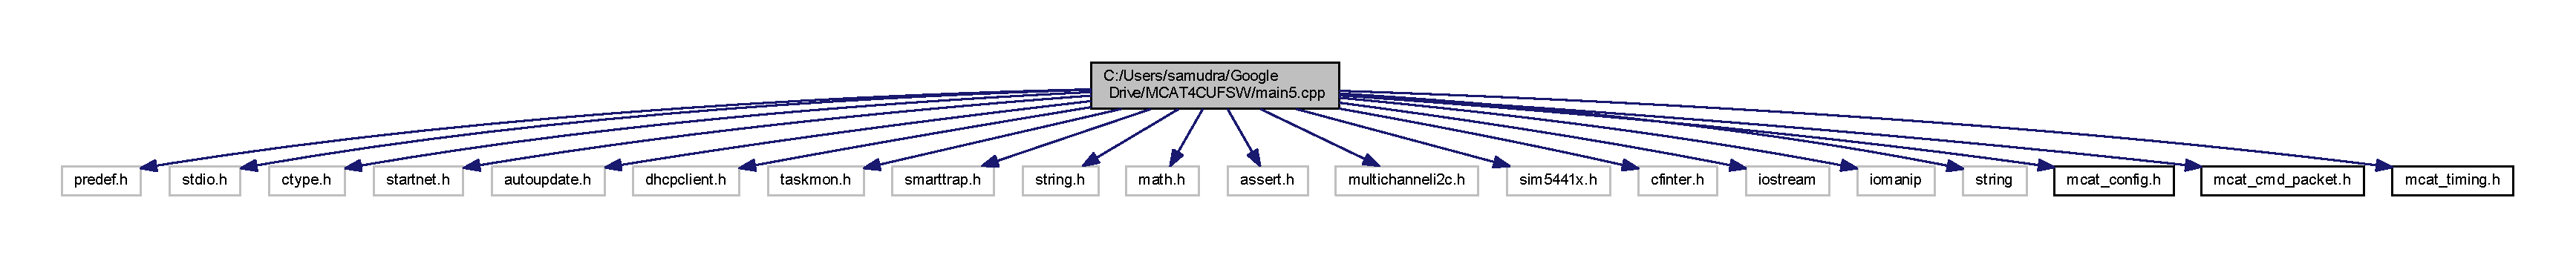
\includegraphics[width=350pt]{main5_8cpp__incl}
\end{center}
\end{figure}
\subsection*{Functions}
\begin{DoxyCompactItemize}
\item 
void \hyperlink{main5_8cpp_af3350bd69feae78ebcd4f766916eeb67}{parse\+C\+M\+D\+Packet} (char C\+M\+D\+Packet\mbox{[}I2\+C\+\_\+\+M\+A\+X\+\_\+\+B\+U\+F\+\_\+\+S\+I\+Z\+E\mbox{]})
\item 
void \hyperlink{main5_8cpp_aa3032893ba2f121a12d4cecf88277580}{parse\+Block\+G} (string Block\+G)
\item 
void \hyperlink{main5_8cpp_ab8ff54f4b027d2dfb6d3b63194fc15a4}{parse\+Block\+C\+U} (string Block\+C\+U)
\item 
void \hyperlink{main5_8cpp_a72e39dd7a2538b8b278f927ffd051bde}{parse\+Block\+I\+P\+D} (string Block\+I\+P\+D)
\item 
void \hyperlink{main5_8cpp_a8109658a433363943c469e7743c238ab}{parse\+Block\+P\+P\+U} (string Block\+P\+P\+U)
\item 
B\+Y\+T\+E \hyperlink{main5_8cpp_a22bb15ed96d4891d904b55838e451124}{Ascii2\+Byte} (char $\ast$buf)
\item 
void \hyperlink{main5_8cpp_ad16e5e62f3579a7048e6b981b172885e}{menu} (void)
\item 
void \hyperlink{main5_8cpp_ace7b2f4c33cbf41f3a43c7be01ff7aec}{User\+Main} (void $\ast$pd)
\item 
void \hyperlink{main5_8cpp_a486c7b37eb37847afaeeb6c73de398b9}{display\+Config} ()
\item 
void \hyperlink{main5_8cpp_a855e0d71fbad695926236f90ac687f35}{do\+Pulses} (void $\ast$pdata)
\item 
void \hyperlink{main5_8cpp_a11ee600b69b27b0bb2d1b5b6e8ece140}{stop\+Pulses} (void $\ast$pdata)
\item 
void \hyperlink{main5_8cpp_a10570e6420ce0f0a076e1e9d3518d305}{init\+D\+M\+A\+T\+I\+M\+E\+R1} ()
\item 
void \hyperlink{main5_8cpp_a7c3f73193878c079945a21075f128059}{Set\+Intc} (long func, int vector, int level, int prio)
\item 
void \hyperlink{main5_8cpp_a8a64466bfb43094b3aec845670b959b4}{set\+Defaults} ()
\item 
void \hyperlink{main5_8cpp_a238885c747f586049b766fa4fcd5ec12}{disable\+All} ()
\item 
void \hyperlink{main5_8cpp_af2e78c1a970cd9490fcc3a5ac8015e6b}{debug\+Print} (string debug\+Msg)
\item 
\hyperlink{main5_8cpp_a89200d64c07024287b4ef31901f44e15}{I\+N\+T\+E\+R\+R\+U\+P\+T} (func\+\_\+isr, 0x2600)
\item 
void \hyperlink{main5_8cpp_acbfa28dfc2a41cc9cea58425f9b75178}{control\+P\+M\+A} (B\+O\+O\+L P\+M\+Flag)
\item 
void \hyperlink{main5_8cpp_ae4e046c7843050c83a5f70092acdbe1d}{control18\+L} (int requested\+Channel, int L\+Flag)
\item 
void \hyperlink{main5_8cpp_ac3f210415061a8b78eaf54a8274ad34a}{control18\+H} (int requested\+Channel, int H\+Flag)
\item 
void \hyperlink{main5_8cpp_a92a0eb6ae19d1612e39cbf1fd318d406}{set\+T\+P1} (long Frequency)
\item 
void \hyperlink{main5_8cpp_a8f5495a6630209795a3fbd7fa61a18e8}{control\+T\+P1} (B\+O\+O\+L T\+P1\+Flag)
\item 
void \hyperlink{main5_8cpp_a0ecec396fb6600a2f4897e7f30318159}{go\+F\+I\+R} ()
\item 
void \hyperlink{main5_8cpp_a2d0df7e0313c78e94bb4fafbc5752d67}{go\+F\+I\+Rfrom\+R\+U\+N} ()
\item 
void \hyperlink{main5_8cpp_ae0014243028b5cd808de963c18d01b11}{go\+F\+I\+Rfrom\+S\+B\+Y} ()
\item 
void \hyperlink{main5_8cpp_affc7dbdeb188c8169ccc6478143538d6}{go\+F\+I\+Rfrom\+I\+D\+L} ()
\item 
void \hyperlink{main5_8cpp_af57dea23daabb0f6e6d27f2ef21c9a54}{go\+R\+U\+N} ()
\item 
void \hyperlink{main5_8cpp_a6d712eb455e679cbf844c6742e7be6a0}{go\+R\+U\+Nfrom\+F\+I\+R} ()
\item 
void \hyperlink{main5_8cpp_a4770c1a01b1be1b23772d600b787d411}{go\+R\+U\+Nfrom\+S\+B\+Y} ()
\item 
void \hyperlink{main5_8cpp_a300391508ed006e4cd4ee0f9f316f3b4}{go\+R\+U\+Nfrom\+I\+D\+L} ()
\item 
void \hyperlink{main5_8cpp_a646dbe8155e1ee44efac5d50a7de878e}{go\+S\+B\+Y} ()
\item 
void \hyperlink{main5_8cpp_ae0ed43b60101aed3be6bea960293275d}{go\+S\+B\+Yfrom\+F\+I\+R} ()
\item 
void \hyperlink{main5_8cpp_a2d0b911e7b667c6a18000005acb28777}{go\+S\+B\+Yfrom\+R\+U\+N} ()
\item 
void \hyperlink{main5_8cpp_a37a57a2b0feb89b22b270931ae440c35}{go\+S\+B\+Yfrom\+I\+D\+L} ()
\item 
void \hyperlink{main5_8cpp_aa8d8f1cf694be5de1ac89b91627c0f51}{go\+I\+D\+L} ()
\item 
void \hyperlink{main5_8cpp_a3e3cc85ab7a91d6808984a0f78a5f9f8}{go\+I\+D\+Lfrom\+S\+B\+Y} ()
\item 
void \hyperlink{main5_8cpp_a690d16feac877ce7000b00e151dffd82}{go\+I\+D\+Lfrom\+R\+U\+N} ()
\item 
void \hyperlink{main5_8cpp_ae5438692f2a6c279129ecc19a91568f2}{go\+I\+D\+Lfrom\+F\+I\+R} ()
\item 
void \hyperlink{main5_8cpp_a9b07c4b395adfe387d12241e7ebaaae6}{set\+New\+Mode} (string cmd\+Mode\+Request, string \hyperlink{main6_c_8cpp_ab996ab5995af95792f5af3586d943d58}{cmd\+Mode\+Current})
\item 
void \hyperlink{main5_8cpp_a5b251dff1da28eda51e8b51bc4b2baf7}{do\+Setup\+I\+O} ()
\end{DoxyCompactItemize}
\subsection*{Variables}
\begin{DoxyCompactItemize}
\item 
string \hyperlink{main5_8cpp_a405cdd34a0ec61abf8c5205c7a8c3182}{cmd\+Version} =\char`\"{}\char`\"{}
\item 
string \hyperlink{main5_8cpp_a8a9767341d04352fccd7068bc1d7c370}{cmd\+Mode} =\char`\"{}\char`\"{}
\item 
string \hyperlink{main5_8cpp_ab996ab5995af95792f5af3586d943d58}{cmd\+Mode\+Current} =\char`\"{}\char`\"{}
\item 
string \hyperlink{main5_8cpp_a56a16ee6139d263a1945acac7412db03}{s\+\_\+cmd\+T\+P1} =\char`\"{}\char`\"{}
\item 
string \hyperlink{main5_8cpp_ac2f7f3d71312267f0daf019326ab81ab}{s\+\_\+cmd\+T\+P2} =\char`\"{}\char`\"{}
\item 
string \hyperlink{main5_8cpp_a684796ab1de60babd3eba75aa8489e68}{s\+\_\+cmd\+T\+P3} =\char`\"{}\char`\"{}
\item 
string \hyperlink{main5_8cpp_a42269eac5fc051ca6c78aae8b6349920}{s\+\_\+cmd\+T\+P4} =\char`\"{}\char`\"{}
\item 
string \hyperlink{main5_8cpp_aa8cec591ab6bc2c30368790b9c90e439}{s\+\_\+cmd\+P\+C\+H1} =\char`\"{}\char`\"{}
\item 
string \hyperlink{main5_8cpp_a0f0135bb7a354979b68358781b0b9a33}{s\+\_\+cmd\+P\+C\+H2} =\char`\"{}\char`\"{}
\item 
string \hyperlink{main5_8cpp_ad027927effdfbc03356897f6784a332f}{s\+\_\+cmd\+P\+C\+H3} =\char`\"{}\char`\"{}
\item 
string \hyperlink{main5_8cpp_a1ee9de883e3c6e7840f6bfd0fdff6976}{s\+\_\+cmd\+P\+C\+H4} =\char`\"{}\char`\"{}
\item 
long \hyperlink{main5_8cpp_ac244c5de67ae1cf2ad9042dd3dd42f5c}{cmd\+T\+P1}
\item 
long \hyperlink{main5_8cpp_a6b5cb6b3c68ceba258ad6741ccf2c2c2}{cmd\+T\+P2}
\item 
long \hyperlink{main5_8cpp_a22ed1f6fb6c9e5132174497269472950}{cmd\+T\+P3}
\item 
long \hyperlink{main5_8cpp_ac556ac861b98bb773707ad78139dd4a7}{cmd\+T\+P4}
\item 
long \hyperlink{main5_8cpp_a6aa9310d261695da6caf50707b289e99}{cmd\+P\+C\+H1}
\item 
long \hyperlink{main5_8cpp_a2ede701ffcc3766012be6e4080433432}{cmd\+P\+C\+H2}
\item 
long \hyperlink{main5_8cpp_a5128aa37f4fea97bace715bd297c7cb4}{cmd\+P\+C\+H3}
\item 
long \hyperlink{main5_8cpp_acda88eaa3c77c003b3a5642a3e28bb48}{cmd\+P\+C\+H4}
\item 
string \hyperlink{main5_8cpp_a37ec136ae86c4b7dc81f393bb1a01af7}{s\+\_\+cmd\+P18\+H1} =\char`\"{}\char`\"{}
\item 
string \hyperlink{main5_8cpp_a46ce373f60085f5900464cd0731fa20e}{s\+\_\+cmd\+P18\+H2} =\char`\"{}\char`\"{}
\item 
string \hyperlink{main5_8cpp_a909acdc96889fb5885793e8bc70b083e}{s\+\_\+cmd\+P18\+H3} =\char`\"{}\char`\"{}
\item 
string \hyperlink{main5_8cpp_a607e82175ad61b864bfa84e686437947}{s\+\_\+cmd\+P18\+H4} =\char`\"{}\char`\"{}
\item 
bool \hyperlink{main5_8cpp_a1a10d6a42e7c3ba1ad7f396b687a7eb7}{cmd\+P18\+H1}
\item 
bool \hyperlink{main5_8cpp_a03df8cc8ee6b4d7ba8a3d2ad50914508}{cmd\+P18\+H2}
\item 
bool \hyperlink{main5_8cpp_aba803fecbea259c5af71f0b9f2e9fa5a}{cmd\+P18\+H3}
\item 
bool \hyperlink{main5_8cpp_a74d16dd0ede9be1a1645027bd2e6fb21}{cmd\+P18\+H4}
\item 
B\+Y\+T\+E \hyperlink{main5_8cpp_a750abfb0120c1735c922980bd47640a5}{buffer} \mbox{[}I2\+C\+\_\+\+M\+A\+X\+\_\+\+B\+U\+F\+\_\+\+S\+I\+Z\+E\mbox{]}
\item 
char \hyperlink{main5_8cpp_af54d77a991da4ba360d594c2589140df}{I2\+C\+Input\+Buffer} \mbox{[}I2\+C\+\_\+\+M\+A\+X\+\_\+\+B\+U\+F\+\_\+\+S\+I\+Z\+E\mbox{]}
\item 
char $\ast$ \hyperlink{main5_8cpp_abed0c40696905e144ed4118061acf700}{inbuf} = \hyperlink{_v2_01main_8cpp_af54d77a991da4ba360d594c2589140df}{I2\+C\+Input\+Buffer}
\item 
B\+Y\+T\+E \hyperlink{main5_8cpp_a92fb5ea5b6a7d108dea33dd07809152d}{address} = \hyperlink{mcatsubsystemconfig_8h_a8fe248bd745b90e2bfe94d8c5fce0a53}{C\+U\+\_\+\+I2\+C\+\_\+\+S\+L\+A\+V\+E\+\_\+\+A\+D\+D\+R}
\item 
B\+Y\+T\+E \hyperlink{main5_8cpp_a6c3dedd37414833dd07e72ee4a642d13}{I2\+C\+Stat}
\end{DoxyCompactItemize}


\subsection{Function Documentation}
\hypertarget{main5_8cpp_a22bb15ed96d4891d904b55838e451124}{}\index{main5.\+cpp@{main5.\+cpp}!Ascii2\+Byte@{Ascii2\+Byte}}
\index{Ascii2\+Byte@{Ascii2\+Byte}!main5.\+cpp@{main5.\+cpp}}
\subsubsection[{Ascii2\+Byte}]{\setlength{\rightskip}{0pt plus 5cm}B\+Y\+T\+E Ascii2\+Byte (
\begin{DoxyParamCaption}
\item[{char $\ast$}]{buf}
\end{DoxyParamCaption}
)}\label{main5_8cpp_a22bb15ed96d4891d904b55838e451124}


Definition at line 914 of file main5.\+cpp.

\hypertarget{main5_8cpp_ac3f210415061a8b78eaf54a8274ad34a}{}\index{main5.\+cpp@{main5.\+cpp}!control18\+H@{control18\+H}}
\index{control18\+H@{control18\+H}!main5.\+cpp@{main5.\+cpp}}
\subsubsection[{control18\+H}]{\setlength{\rightskip}{0pt plus 5cm}void control18\+H (
\begin{DoxyParamCaption}
\item[{int}]{requested\+Channel, }
\item[{int}]{H\+Flag}
\end{DoxyParamCaption}
)}\label{main5_8cpp_ac3f210415061a8b78eaf54a8274ad34a}


Definition at line 331 of file main5.\+cpp.

\hypertarget{main5_8cpp_ae4e046c7843050c83a5f70092acdbe1d}{}\index{main5.\+cpp@{main5.\+cpp}!control18\+L@{control18\+L}}
\index{control18\+L@{control18\+L}!main5.\+cpp@{main5.\+cpp}}
\subsubsection[{control18\+L}]{\setlength{\rightskip}{0pt plus 5cm}void control18\+L (
\begin{DoxyParamCaption}
\item[{int}]{requested\+Channel, }
\item[{int}]{L\+Flag}
\end{DoxyParamCaption}
)}\label{main5_8cpp_ae4e046c7843050c83a5f70092acdbe1d}


Definition at line 268 of file main5.\+cpp.

\hypertarget{main5_8cpp_acbfa28dfc2a41cc9cea58425f9b75178}{}\index{main5.\+cpp@{main5.\+cpp}!control\+P\+M\+A@{control\+P\+M\+A}}
\index{control\+P\+M\+A@{control\+P\+M\+A}!main5.\+cpp@{main5.\+cpp}}
\subsubsection[{control\+P\+M\+A}]{\setlength{\rightskip}{0pt plus 5cm}void control\+P\+M\+A (
\begin{DoxyParamCaption}
\item[{B\+O\+O\+L}]{P\+M\+Flag}
\end{DoxyParamCaption}
)}\label{main5_8cpp_acbfa28dfc2a41cc9cea58425f9b75178}


Definition at line 252 of file main5.\+cpp.

\hypertarget{main5_8cpp_a8f5495a6630209795a3fbd7fa61a18e8}{}\index{main5.\+cpp@{main5.\+cpp}!control\+T\+P1@{control\+T\+P1}}
\index{control\+T\+P1@{control\+T\+P1}!main5.\+cpp@{main5.\+cpp}}
\subsubsection[{control\+T\+P1}]{\setlength{\rightskip}{0pt plus 5cm}void control\+T\+P1 (
\begin{DoxyParamCaption}
\item[{B\+O\+O\+L}]{T\+P1\+Flag}
\end{DoxyParamCaption}
)}\label{main5_8cpp_a8f5495a6630209795a3fbd7fa61a18e8}
from 5270 code set /// D\+O N\+O\+T U\+S\+E Set\+Intc((long) \&func\+\_\+isr, 19, 1, 1); 

Definition at line 420 of file main5.\+cpp.

\hypertarget{main5_8cpp_af2e78c1a970cd9490fcc3a5ac8015e6b}{}\index{main5.\+cpp@{main5.\+cpp}!debug\+Print@{debug\+Print}}
\index{debug\+Print@{debug\+Print}!main5.\+cpp@{main5.\+cpp}}
\subsubsection[{debug\+Print}]{\setlength{\rightskip}{0pt plus 5cm}void debug\+Print (
\begin{DoxyParamCaption}
\item[{string}]{debug\+Msg}
\end{DoxyParamCaption}
)}\label{main5_8cpp_af2e78c1a970cd9490fcc3a5ac8015e6b}


Definition at line 177 of file main5.\+cpp.

\hypertarget{main5_8cpp_a238885c747f586049b766fa4fcd5ec12}{}\index{main5.\+cpp@{main5.\+cpp}!disable\+All@{disable\+All}}
\index{disable\+All@{disable\+All}!main5.\+cpp@{main5.\+cpp}}
\subsubsection[{disable\+All}]{\setlength{\rightskip}{0pt plus 5cm}void disable\+All (
\begin{DoxyParamCaption}
{}
\end{DoxyParamCaption}
)}\label{main5_8cpp_a238885c747f586049b766fa4fcd5ec12}


Definition at line 609 of file main5.\+cpp.

\hypertarget{main5_8cpp_a486c7b37eb37847afaeeb6c73de398b9}{}\index{main5.\+cpp@{main5.\+cpp}!display\+Config@{display\+Config}}
\index{display\+Config@{display\+Config}!main5.\+cpp@{main5.\+cpp}}
\subsubsection[{display\+Config}]{\setlength{\rightskip}{0pt plus 5cm}void display\+Config (
\begin{DoxyParamCaption}
{}
\end{DoxyParamCaption}
)}\label{main5_8cpp_a486c7b37eb37847afaeeb6c73de398b9}
\hypertarget{main5_8cpp_a855e0d71fbad695926236f90ac687f35}{}\index{main5.\+cpp@{main5.\+cpp}!do\+Pulses@{do\+Pulses}}
\index{do\+Pulses@{do\+Pulses}!main5.\+cpp@{main5.\+cpp}}
\subsubsection[{do\+Pulses}]{\setlength{\rightskip}{0pt plus 5cm}void do\+Pulses (
\begin{DoxyParamCaption}
\item[{void $\ast$}]{pdata}
\end{DoxyParamCaption}
)}\label{main5_8cpp_a855e0d71fbad695926236f90ac687f35}


Definition at line 627 of file main5.\+cpp.

\hypertarget{main5_8cpp_a5b251dff1da28eda51e8b51bc4b2baf7}{}\index{main5.\+cpp@{main5.\+cpp}!do\+Setup\+I\+O@{do\+Setup\+I\+O}}
\index{do\+Setup\+I\+O@{do\+Setup\+I\+O}!main5.\+cpp@{main5.\+cpp}}
\subsubsection[{do\+Setup\+I\+O}]{\setlength{\rightskip}{0pt plus 5cm}void do\+Setup\+I\+O (
\begin{DoxyParamCaption}
{}
\end{DoxyParamCaption}
)}\label{main5_8cpp_a5b251dff1da28eda51e8b51bc4b2baf7}


Definition at line 670 of file main5.\+cpp.

\hypertarget{main5_8cpp_a0ecec396fb6600a2f4897e7f30318159}{}\index{main5.\+cpp@{main5.\+cpp}!go\+F\+I\+R@{go\+F\+I\+R}}
\index{go\+F\+I\+R@{go\+F\+I\+R}!main5.\+cpp@{main5.\+cpp}}
\subsubsection[{go\+F\+I\+R}]{\setlength{\rightskip}{0pt plus 5cm}void go\+F\+I\+R (
\begin{DoxyParamCaption}
{}
\end{DoxyParamCaption}
)}\label{main5_8cpp_a0ecec396fb6600a2f4897e7f30318159}


Definition at line 454 of file main5.\+cpp.

\hypertarget{main5_8cpp_affc7dbdeb188c8169ccc6478143538d6}{}\index{main5.\+cpp@{main5.\+cpp}!go\+F\+I\+Rfrom\+I\+D\+L@{go\+F\+I\+Rfrom\+I\+D\+L}}
\index{go\+F\+I\+Rfrom\+I\+D\+L@{go\+F\+I\+Rfrom\+I\+D\+L}!main5.\+cpp@{main5.\+cpp}}
\subsubsection[{go\+F\+I\+Rfrom\+I\+D\+L}]{\setlength{\rightskip}{0pt plus 5cm}void go\+F\+I\+Rfrom\+I\+D\+L (
\begin{DoxyParamCaption}
{}
\end{DoxyParamCaption}
)}\label{main5_8cpp_affc7dbdeb188c8169ccc6478143538d6}


Definition at line 467 of file main5.\+cpp.

\hypertarget{main5_8cpp_a2d0df7e0313c78e94bb4fafbc5752d67}{}\index{main5.\+cpp@{main5.\+cpp}!go\+F\+I\+Rfrom\+R\+U\+N@{go\+F\+I\+Rfrom\+R\+U\+N}}
\index{go\+F\+I\+Rfrom\+R\+U\+N@{go\+F\+I\+Rfrom\+R\+U\+N}!main5.\+cpp@{main5.\+cpp}}
\subsubsection[{go\+F\+I\+Rfrom\+R\+U\+N}]{\setlength{\rightskip}{0pt plus 5cm}void go\+F\+I\+Rfrom\+R\+U\+N (
\begin{DoxyParamCaption}
{}
\end{DoxyParamCaption}
)}\label{main5_8cpp_a2d0df7e0313c78e94bb4fafbc5752d67}


Definition at line 459 of file main5.\+cpp.

\hypertarget{main5_8cpp_ae0014243028b5cd808de963c18d01b11}{}\index{main5.\+cpp@{main5.\+cpp}!go\+F\+I\+Rfrom\+S\+B\+Y@{go\+F\+I\+Rfrom\+S\+B\+Y}}
\index{go\+F\+I\+Rfrom\+S\+B\+Y@{go\+F\+I\+Rfrom\+S\+B\+Y}!main5.\+cpp@{main5.\+cpp}}
\subsubsection[{go\+F\+I\+Rfrom\+S\+B\+Y}]{\setlength{\rightskip}{0pt plus 5cm}void go\+F\+I\+Rfrom\+S\+B\+Y (
\begin{DoxyParamCaption}
{}
\end{DoxyParamCaption}
)}\label{main5_8cpp_ae0014243028b5cd808de963c18d01b11}


Definition at line 463 of file main5.\+cpp.

\hypertarget{main5_8cpp_aa8d8f1cf694be5de1ac89b91627c0f51}{}\index{main5.\+cpp@{main5.\+cpp}!go\+I\+D\+L@{go\+I\+D\+L}}
\index{go\+I\+D\+L@{go\+I\+D\+L}!main5.\+cpp@{main5.\+cpp}}
\subsubsection[{go\+I\+D\+L}]{\setlength{\rightskip}{0pt plus 5cm}void go\+I\+D\+L (
\begin{DoxyParamCaption}
{}
\end{DoxyParamCaption}
)}\label{main5_8cpp_aa8d8f1cf694be5de1ac89b91627c0f51}


Definition at line 512 of file main5.\+cpp.

\hypertarget{main5_8cpp_ae5438692f2a6c279129ecc19a91568f2}{}\index{main5.\+cpp@{main5.\+cpp}!go\+I\+D\+Lfrom\+F\+I\+R@{go\+I\+D\+Lfrom\+F\+I\+R}}
\index{go\+I\+D\+Lfrom\+F\+I\+R@{go\+I\+D\+Lfrom\+F\+I\+R}!main5.\+cpp@{main5.\+cpp}}
\subsubsection[{go\+I\+D\+Lfrom\+F\+I\+R}]{\setlength{\rightskip}{0pt plus 5cm}void go\+I\+D\+Lfrom\+F\+I\+R (
\begin{DoxyParamCaption}
{}
\end{DoxyParamCaption}
)}\label{main5_8cpp_ae5438692f2a6c279129ecc19a91568f2}


Definition at line 525 of file main5.\+cpp.

\hypertarget{main5_8cpp_a690d16feac877ce7000b00e151dffd82}{}\index{main5.\+cpp@{main5.\+cpp}!go\+I\+D\+Lfrom\+R\+U\+N@{go\+I\+D\+Lfrom\+R\+U\+N}}
\index{go\+I\+D\+Lfrom\+R\+U\+N@{go\+I\+D\+Lfrom\+R\+U\+N}!main5.\+cpp@{main5.\+cpp}}
\subsubsection[{go\+I\+D\+Lfrom\+R\+U\+N}]{\setlength{\rightskip}{0pt plus 5cm}void go\+I\+D\+Lfrom\+R\+U\+N (
\begin{DoxyParamCaption}
{}
\end{DoxyParamCaption}
)}\label{main5_8cpp_a690d16feac877ce7000b00e151dffd82}


Definition at line 521 of file main5.\+cpp.

\hypertarget{main5_8cpp_a3e3cc85ab7a91d6808984a0f78a5f9f8}{}\index{main5.\+cpp@{main5.\+cpp}!go\+I\+D\+Lfrom\+S\+B\+Y@{go\+I\+D\+Lfrom\+S\+B\+Y}}
\index{go\+I\+D\+Lfrom\+S\+B\+Y@{go\+I\+D\+Lfrom\+S\+B\+Y}!main5.\+cpp@{main5.\+cpp}}
\subsubsection[{go\+I\+D\+Lfrom\+S\+B\+Y}]{\setlength{\rightskip}{0pt plus 5cm}void go\+I\+D\+Lfrom\+S\+B\+Y (
\begin{DoxyParamCaption}
{}
\end{DoxyParamCaption}
)}\label{main5_8cpp_a3e3cc85ab7a91d6808984a0f78a5f9f8}


Definition at line 517 of file main5.\+cpp.

\hypertarget{main5_8cpp_af57dea23daabb0f6e6d27f2ef21c9a54}{}\index{main5.\+cpp@{main5.\+cpp}!go\+R\+U\+N@{go\+R\+U\+N}}
\index{go\+R\+U\+N@{go\+R\+U\+N}!main5.\+cpp@{main5.\+cpp}}
\subsubsection[{go\+R\+U\+N}]{\setlength{\rightskip}{0pt plus 5cm}void go\+R\+U\+N (
\begin{DoxyParamCaption}
{}
\end{DoxyParamCaption}
)}\label{main5_8cpp_af57dea23daabb0f6e6d27f2ef21c9a54}


Definition at line 472 of file main5.\+cpp.

\hypertarget{main5_8cpp_a6d712eb455e679cbf844c6742e7be6a0}{}\index{main5.\+cpp@{main5.\+cpp}!go\+R\+U\+Nfrom\+F\+I\+R@{go\+R\+U\+Nfrom\+F\+I\+R}}
\index{go\+R\+U\+Nfrom\+F\+I\+R@{go\+R\+U\+Nfrom\+F\+I\+R}!main5.\+cpp@{main5.\+cpp}}
\subsubsection[{go\+R\+U\+Nfrom\+F\+I\+R}]{\setlength{\rightskip}{0pt plus 5cm}void go\+R\+U\+Nfrom\+F\+I\+R (
\begin{DoxyParamCaption}
{}
\end{DoxyParamCaption}
)}\label{main5_8cpp_a6d712eb455e679cbf844c6742e7be6a0}


Definition at line 481 of file main5.\+cpp.

\hypertarget{main5_8cpp_a300391508ed006e4cd4ee0f9f316f3b4}{}\index{main5.\+cpp@{main5.\+cpp}!go\+R\+U\+Nfrom\+I\+D\+L@{go\+R\+U\+Nfrom\+I\+D\+L}}
\index{go\+R\+U\+Nfrom\+I\+D\+L@{go\+R\+U\+Nfrom\+I\+D\+L}!main5.\+cpp@{main5.\+cpp}}
\subsubsection[{go\+R\+U\+Nfrom\+I\+D\+L}]{\setlength{\rightskip}{0pt plus 5cm}void go\+R\+U\+Nfrom\+I\+D\+L (
\begin{DoxyParamCaption}
{}
\end{DoxyParamCaption}
)}\label{main5_8cpp_a300391508ed006e4cd4ee0f9f316f3b4}


Definition at line 489 of file main5.\+cpp.

\hypertarget{main5_8cpp_a4770c1a01b1be1b23772d600b787d411}{}\index{main5.\+cpp@{main5.\+cpp}!go\+R\+U\+Nfrom\+S\+B\+Y@{go\+R\+U\+Nfrom\+S\+B\+Y}}
\index{go\+R\+U\+Nfrom\+S\+B\+Y@{go\+R\+U\+Nfrom\+S\+B\+Y}!main5.\+cpp@{main5.\+cpp}}
\subsubsection[{go\+R\+U\+Nfrom\+S\+B\+Y}]{\setlength{\rightskip}{0pt plus 5cm}void go\+R\+U\+Nfrom\+S\+B\+Y (
\begin{DoxyParamCaption}
{}
\end{DoxyParamCaption}
)}\label{main5_8cpp_a4770c1a01b1be1b23772d600b787d411}


Definition at line 485 of file main5.\+cpp.

\hypertarget{main5_8cpp_a646dbe8155e1ee44efac5d50a7de878e}{}\index{main5.\+cpp@{main5.\+cpp}!go\+S\+B\+Y@{go\+S\+B\+Y}}
\index{go\+S\+B\+Y@{go\+S\+B\+Y}!main5.\+cpp@{main5.\+cpp}}
\subsubsection[{go\+S\+B\+Y}]{\setlength{\rightskip}{0pt plus 5cm}void go\+S\+B\+Y (
\begin{DoxyParamCaption}
{}
\end{DoxyParamCaption}
)}\label{main5_8cpp_a646dbe8155e1ee44efac5d50a7de878e}


Definition at line 494 of file main5.\+cpp.

\hypertarget{main5_8cpp_ae0ed43b60101aed3be6bea960293275d}{}\index{main5.\+cpp@{main5.\+cpp}!go\+S\+B\+Yfrom\+F\+I\+R@{go\+S\+B\+Yfrom\+F\+I\+R}}
\index{go\+S\+B\+Yfrom\+F\+I\+R@{go\+S\+B\+Yfrom\+F\+I\+R}!main5.\+cpp@{main5.\+cpp}}
\subsubsection[{go\+S\+B\+Yfrom\+F\+I\+R}]{\setlength{\rightskip}{0pt plus 5cm}void go\+S\+B\+Yfrom\+F\+I\+R (
\begin{DoxyParamCaption}
{}
\end{DoxyParamCaption}
)}\label{main5_8cpp_ae0ed43b60101aed3be6bea960293275d}


Definition at line 499 of file main5.\+cpp.

\hypertarget{main5_8cpp_a37a57a2b0feb89b22b270931ae440c35}{}\index{main5.\+cpp@{main5.\+cpp}!go\+S\+B\+Yfrom\+I\+D\+L@{go\+S\+B\+Yfrom\+I\+D\+L}}
\index{go\+S\+B\+Yfrom\+I\+D\+L@{go\+S\+B\+Yfrom\+I\+D\+L}!main5.\+cpp@{main5.\+cpp}}
\subsubsection[{go\+S\+B\+Yfrom\+I\+D\+L}]{\setlength{\rightskip}{0pt plus 5cm}void go\+S\+B\+Yfrom\+I\+D\+L (
\begin{DoxyParamCaption}
{}
\end{DoxyParamCaption}
)}\label{main5_8cpp_a37a57a2b0feb89b22b270931ae440c35}


Definition at line 507 of file main5.\+cpp.

\hypertarget{main5_8cpp_a2d0b911e7b667c6a18000005acb28777}{}\index{main5.\+cpp@{main5.\+cpp}!go\+S\+B\+Yfrom\+R\+U\+N@{go\+S\+B\+Yfrom\+R\+U\+N}}
\index{go\+S\+B\+Yfrom\+R\+U\+N@{go\+S\+B\+Yfrom\+R\+U\+N}!main5.\+cpp@{main5.\+cpp}}
\subsubsection[{go\+S\+B\+Yfrom\+R\+U\+N}]{\setlength{\rightskip}{0pt plus 5cm}void go\+S\+B\+Yfrom\+R\+U\+N (
\begin{DoxyParamCaption}
{}
\end{DoxyParamCaption}
)}\label{main5_8cpp_a2d0b911e7b667c6a18000005acb28777}


Definition at line 503 of file main5.\+cpp.

\hypertarget{main5_8cpp_a10570e6420ce0f0a076e1e9d3518d305}{}\index{main5.\+cpp@{main5.\+cpp}!init\+D\+M\+A\+T\+I\+M\+E\+R1@{init\+D\+M\+A\+T\+I\+M\+E\+R1}}
\index{init\+D\+M\+A\+T\+I\+M\+E\+R1@{init\+D\+M\+A\+T\+I\+M\+E\+R1}!main5.\+cpp@{main5.\+cpp}}
\subsubsection[{init\+D\+M\+A\+T\+I\+M\+E\+R1}]{\setlength{\rightskip}{0pt plus 5cm}void init\+D\+M\+A\+T\+I\+M\+E\+R1 (
\begin{DoxyParamCaption}
{}
\end{DoxyParamCaption}
)}\label{main5_8cpp_a10570e6420ce0f0a076e1e9d3518d305}
from 5270 code set /// D\+O N\+O\+T U\+S\+E Set\+Intc((long) \&func\+\_\+isr, 19, 1, 1); 

Definition at line 655 of file main5.\+cpp.

\hypertarget{main5_8cpp_a89200d64c07024287b4ef31901f44e15}{}\index{main5.\+cpp@{main5.\+cpp}!I\+N\+T\+E\+R\+R\+U\+P\+T@{I\+N\+T\+E\+R\+R\+U\+P\+T}}
\index{I\+N\+T\+E\+R\+R\+U\+P\+T@{I\+N\+T\+E\+R\+R\+U\+P\+T}!main5.\+cpp@{main5.\+cpp}}
\subsubsection[{I\+N\+T\+E\+R\+R\+U\+P\+T}]{\setlength{\rightskip}{0pt plus 5cm}I\+N\+T\+E\+R\+R\+U\+P\+T (
\begin{DoxyParamCaption}
\item[{func\+\_\+isr}]{, }
\item[{0x2600}]{}
\end{DoxyParamCaption}
)}\label{main5_8cpp_a89200d64c07024287b4ef31901f44e15}


Definition at line 185 of file main5.\+cpp.

\hypertarget{main5_8cpp_ad16e5e62f3579a7048e6b981b172885e}{}\index{main5.\+cpp@{main5.\+cpp}!menu@{menu}}
\index{menu@{menu}!main5.\+cpp@{main5.\+cpp}}
\subsubsection[{menu}]{\setlength{\rightskip}{0pt plus 5cm}void menu (
\begin{DoxyParamCaption}
\item[{void}]{}
\end{DoxyParamCaption}
)}\label{main5_8cpp_ad16e5e62f3579a7048e6b981b172885e}


Definition at line 932 of file main5.\+cpp.

\hypertarget{main5_8cpp_ab8ff54f4b027d2dfb6d3b63194fc15a4}{}\index{main5.\+cpp@{main5.\+cpp}!parse\+Block\+C\+U@{parse\+Block\+C\+U}}
\index{parse\+Block\+C\+U@{parse\+Block\+C\+U}!main5.\+cpp@{main5.\+cpp}}
\subsubsection[{parse\+Block\+C\+U}]{\setlength{\rightskip}{0pt plus 5cm}void parse\+Block\+C\+U (
\begin{DoxyParamCaption}
\item[{string}]{Block\+C\+U}
\end{DoxyParamCaption}
)}\label{main5_8cpp_ab8ff54f4b027d2dfb6d3b63194fc15a4}


Definition at line 792 of file main5.\+cpp.

\hypertarget{main5_8cpp_aa3032893ba2f121a12d4cecf88277580}{}\index{main5.\+cpp@{main5.\+cpp}!parse\+Block\+G@{parse\+Block\+G}}
\index{parse\+Block\+G@{parse\+Block\+G}!main5.\+cpp@{main5.\+cpp}}
\subsubsection[{parse\+Block\+G}]{\setlength{\rightskip}{0pt plus 5cm}void parse\+Block\+G (
\begin{DoxyParamCaption}
\item[{string}]{Block\+G}
\end{DoxyParamCaption}
)}\label{main5_8cpp_aa3032893ba2f121a12d4cecf88277580}


Definition at line 782 of file main5.\+cpp.

\hypertarget{main5_8cpp_a72e39dd7a2538b8b278f927ffd051bde}{}\index{main5.\+cpp@{main5.\+cpp}!parse\+Block\+I\+P\+D@{parse\+Block\+I\+P\+D}}
\index{parse\+Block\+I\+P\+D@{parse\+Block\+I\+P\+D}!main5.\+cpp@{main5.\+cpp}}
\subsubsection[{parse\+Block\+I\+P\+D}]{\setlength{\rightskip}{0pt plus 5cm}void parse\+Block\+I\+P\+D (
\begin{DoxyParamCaption}
\item[{string}]{Block\+I\+P\+D}
\end{DoxyParamCaption}
)}\label{main5_8cpp_a72e39dd7a2538b8b278f927ffd051bde}


Definition at line 802 of file main5.\+cpp.

\hypertarget{main5_8cpp_a8109658a433363943c469e7743c238ab}{}\index{main5.\+cpp@{main5.\+cpp}!parse\+Block\+P\+P\+U@{parse\+Block\+P\+P\+U}}
\index{parse\+Block\+P\+P\+U@{parse\+Block\+P\+P\+U}!main5.\+cpp@{main5.\+cpp}}
\subsubsection[{parse\+Block\+P\+P\+U}]{\setlength{\rightskip}{0pt plus 5cm}void parse\+Block\+P\+P\+U (
\begin{DoxyParamCaption}
\item[{string}]{Block\+P\+P\+U}
\end{DoxyParamCaption}
)}\label{main5_8cpp_a8109658a433363943c469e7743c238ab}


Definition at line 857 of file main5.\+cpp.

\hypertarget{main5_8cpp_af3350bd69feae78ebcd4f766916eeb67}{}\index{main5.\+cpp@{main5.\+cpp}!parse\+C\+M\+D\+Packet@{parse\+C\+M\+D\+Packet}}
\index{parse\+C\+M\+D\+Packet@{parse\+C\+M\+D\+Packet}!main5.\+cpp@{main5.\+cpp}}
\subsubsection[{parse\+C\+M\+D\+Packet}]{\setlength{\rightskip}{0pt plus 5cm}void parse\+C\+M\+D\+Packet (
\begin{DoxyParamCaption}
\item[{char}]{C\+M\+D\+Packet\mbox{[}\+I2\+C\+\_\+\+M\+A\+X\+\_\+\+B\+U\+F\+\_\+\+S\+I\+Z\+E\mbox{]}}
\end{DoxyParamCaption}
)}\label{main5_8cpp_af3350bd69feae78ebcd4f766916eeb67}


Definition at line 721 of file main5.\+cpp.

\hypertarget{main5_8cpp_a8a64466bfb43094b3aec845670b959b4}{}\index{main5.\+cpp@{main5.\+cpp}!set\+Defaults@{set\+Defaults}}
\index{set\+Defaults@{set\+Defaults}!main5.\+cpp@{main5.\+cpp}}
\subsubsection[{set\+Defaults}]{\setlength{\rightskip}{0pt plus 5cm}void set\+Defaults (
\begin{DoxyParamCaption}
{}
\end{DoxyParamCaption}
)}\label{main5_8cpp_a8a64466bfb43094b3aec845670b959b4}


Definition at line 616 of file main5.\+cpp.

\hypertarget{main5_8cpp_a7c3f73193878c079945a21075f128059}{}\index{main5.\+cpp@{main5.\+cpp}!Set\+Intc@{Set\+Intc}}
\index{Set\+Intc@{Set\+Intc}!main5.\+cpp@{main5.\+cpp}}
\subsubsection[{Set\+Intc}]{\setlength{\rightskip}{0pt plus 5cm}void Set\+Intc (
\begin{DoxyParamCaption}
\item[{long}]{func, }
\item[{int}]{vector, }
\item[{int}]{level, }
\item[{int}]{prio}
\end{DoxyParamCaption}
)}\label{main5_8cpp_a7c3f73193878c079945a21075f128059}
\hypertarget{main5_8cpp_a9b07c4b395adfe387d12241e7ebaaae6}{}\index{main5.\+cpp@{main5.\+cpp}!set\+New\+Mode@{set\+New\+Mode}}
\index{set\+New\+Mode@{set\+New\+Mode}!main5.\+cpp@{main5.\+cpp}}
\subsubsection[{set\+New\+Mode}]{\setlength{\rightskip}{0pt plus 5cm}void set\+New\+Mode (
\begin{DoxyParamCaption}
\item[{string}]{cmd\+Mode\+Request, }
\item[{string}]{cmd\+Mode\+Current}
\end{DoxyParamCaption}
)}\label{main5_8cpp_a9b07c4b395adfe387d12241e7ebaaae6}


Definition at line 532 of file main5.\+cpp.

\hypertarget{main5_8cpp_a92a0eb6ae19d1612e39cbf1fd318d406}{}\index{main5.\+cpp@{main5.\+cpp}!set\+T\+P1@{set\+T\+P1}}
\index{set\+T\+P1@{set\+T\+P1}!main5.\+cpp@{main5.\+cpp}}
\subsubsection[{set\+T\+P1}]{\setlength{\rightskip}{0pt plus 5cm}void set\+T\+P1 (
\begin{DoxyParamCaption}
\item[{long}]{Frequency}
\end{DoxyParamCaption}
)}\label{main5_8cpp_a92a0eb6ae19d1612e39cbf1fd318d406}


Definition at line 399 of file main5.\+cpp.

\hypertarget{main5_8cpp_a11ee600b69b27b0bb2d1b5b6e8ece140}{}\index{main5.\+cpp@{main5.\+cpp}!stop\+Pulses@{stop\+Pulses}}
\index{stop\+Pulses@{stop\+Pulses}!main5.\+cpp@{main5.\+cpp}}
\subsubsection[{stop\+Pulses}]{\setlength{\rightskip}{0pt plus 5cm}void stop\+Pulses (
\begin{DoxyParamCaption}
\item[{void $\ast$}]{pdata}
\end{DoxyParamCaption}
)}\label{main5_8cpp_a11ee600b69b27b0bb2d1b5b6e8ece140}
\hypertarget{main5_8cpp_ace7b2f4c33cbf41f3a43c7be01ff7aec}{}\index{main5.\+cpp@{main5.\+cpp}!User\+Main@{User\+Main}}
\index{User\+Main@{User\+Main}!main5.\+cpp@{main5.\+cpp}}
\subsubsection[{User\+Main}]{\setlength{\rightskip}{0pt plus 5cm}void User\+Main (
\begin{DoxyParamCaption}
\item[{void $\ast$}]{pd}
\end{DoxyParamCaption}
)}\label{main5_8cpp_ace7b2f4c33cbf41f3a43c7be01ff7aec}
Thruster Channel P18 activation section

C\+H1-\/4

End Thruster Channel P18 activation section 

Definition at line 957 of file main5.\+cpp.



\subsection{Variable Documentation}
\hypertarget{main5_8cpp_a92fb5ea5b6a7d108dea33dd07809152d}{}\index{main5.\+cpp@{main5.\+cpp}!address@{address}}
\index{address@{address}!main5.\+cpp@{main5.\+cpp}}
\subsubsection[{address}]{\setlength{\rightskip}{0pt plus 5cm}B\+Y\+T\+E address = {\bf C\+U\+\_\+\+I2\+C\+\_\+\+S\+L\+A\+V\+E\+\_\+\+A\+D\+D\+R}}\label{main5_8cpp_a92fb5ea5b6a7d108dea33dd07809152d}


Definition at line 174 of file main5.\+cpp.

\hypertarget{main5_8cpp_a750abfb0120c1735c922980bd47640a5}{}\index{main5.\+cpp@{main5.\+cpp}!buffer@{buffer}}
\index{buffer@{buffer}!main5.\+cpp@{main5.\+cpp}}
\subsubsection[{buffer}]{\setlength{\rightskip}{0pt plus 5cm}B\+Y\+T\+E buffer\mbox{[}I2\+C\+\_\+\+M\+A\+X\+\_\+\+B\+U\+F\+\_\+\+S\+I\+Z\+E\mbox{]}}\label{main5_8cpp_a750abfb0120c1735c922980bd47640a5}


Definition at line 171 of file main5.\+cpp.

\hypertarget{main5_8cpp_a8a9767341d04352fccd7068bc1d7c370}{}\index{main5.\+cpp@{main5.\+cpp}!cmd\+Mode@{cmd\+Mode}}
\index{cmd\+Mode@{cmd\+Mode}!main5.\+cpp@{main5.\+cpp}}
\subsubsection[{cmd\+Mode}]{\setlength{\rightskip}{0pt plus 5cm}string cmd\+Mode =\char`\"{}\char`\"{}}\label{main5_8cpp_a8a9767341d04352fccd7068bc1d7c370}


Definition at line 101 of file main5.\+cpp.

\hypertarget{main5_8cpp_ab996ab5995af95792f5af3586d943d58}{}\index{main5.\+cpp@{main5.\+cpp}!cmd\+Mode\+Current@{cmd\+Mode\+Current}}
\index{cmd\+Mode\+Current@{cmd\+Mode\+Current}!main5.\+cpp@{main5.\+cpp}}
\subsubsection[{cmd\+Mode\+Current}]{\setlength{\rightskip}{0pt plus 5cm}string cmd\+Mode\+Current =\char`\"{}\char`\"{}}\label{main5_8cpp_ab996ab5995af95792f5af3586d943d58}


Definition at line 102 of file main5.\+cpp.

\hypertarget{main5_8cpp_a1a10d6a42e7c3ba1ad7f396b687a7eb7}{}\index{main5.\+cpp@{main5.\+cpp}!cmd\+P18\+H1@{cmd\+P18\+H1}}
\index{cmd\+P18\+H1@{cmd\+P18\+H1}!main5.\+cpp@{main5.\+cpp}}
\subsubsection[{cmd\+P18\+H1}]{\setlength{\rightskip}{0pt plus 5cm}bool cmd\+P18\+H1}\label{main5_8cpp_a1a10d6a42e7c3ba1ad7f396b687a7eb7}


Definition at line 116 of file main5.\+cpp.

\hypertarget{main5_8cpp_a03df8cc8ee6b4d7ba8a3d2ad50914508}{}\index{main5.\+cpp@{main5.\+cpp}!cmd\+P18\+H2@{cmd\+P18\+H2}}
\index{cmd\+P18\+H2@{cmd\+P18\+H2}!main5.\+cpp@{main5.\+cpp}}
\subsubsection[{cmd\+P18\+H2}]{\setlength{\rightskip}{0pt plus 5cm}bool cmd\+P18\+H2}\label{main5_8cpp_a03df8cc8ee6b4d7ba8a3d2ad50914508}


Definition at line 116 of file main5.\+cpp.

\hypertarget{main5_8cpp_aba803fecbea259c5af71f0b9f2e9fa5a}{}\index{main5.\+cpp@{main5.\+cpp}!cmd\+P18\+H3@{cmd\+P18\+H3}}
\index{cmd\+P18\+H3@{cmd\+P18\+H3}!main5.\+cpp@{main5.\+cpp}}
\subsubsection[{cmd\+P18\+H3}]{\setlength{\rightskip}{0pt plus 5cm}bool cmd\+P18\+H3}\label{main5_8cpp_aba803fecbea259c5af71f0b9f2e9fa5a}


Definition at line 116 of file main5.\+cpp.

\hypertarget{main5_8cpp_a74d16dd0ede9be1a1645027bd2e6fb21}{}\index{main5.\+cpp@{main5.\+cpp}!cmd\+P18\+H4@{cmd\+P18\+H4}}
\index{cmd\+P18\+H4@{cmd\+P18\+H4}!main5.\+cpp@{main5.\+cpp}}
\subsubsection[{cmd\+P18\+H4}]{\setlength{\rightskip}{0pt plus 5cm}bool cmd\+P18\+H4}\label{main5_8cpp_a74d16dd0ede9be1a1645027bd2e6fb21}


Definition at line 116 of file main5.\+cpp.

\hypertarget{main5_8cpp_a6aa9310d261695da6caf50707b289e99}{}\index{main5.\+cpp@{main5.\+cpp}!cmd\+P\+C\+H1@{cmd\+P\+C\+H1}}
\index{cmd\+P\+C\+H1@{cmd\+P\+C\+H1}!main5.\+cpp@{main5.\+cpp}}
\subsubsection[{cmd\+P\+C\+H1}]{\setlength{\rightskip}{0pt plus 5cm}long cmd\+P\+C\+H1}\label{main5_8cpp_a6aa9310d261695da6caf50707b289e99}


Definition at line 111 of file main5.\+cpp.

\hypertarget{main5_8cpp_a2ede701ffcc3766012be6e4080433432}{}\index{main5.\+cpp@{main5.\+cpp}!cmd\+P\+C\+H2@{cmd\+P\+C\+H2}}
\index{cmd\+P\+C\+H2@{cmd\+P\+C\+H2}!main5.\+cpp@{main5.\+cpp}}
\subsubsection[{cmd\+P\+C\+H2}]{\setlength{\rightskip}{0pt plus 5cm}long cmd\+P\+C\+H2}\label{main5_8cpp_a2ede701ffcc3766012be6e4080433432}


Definition at line 111 of file main5.\+cpp.

\hypertarget{main5_8cpp_a5128aa37f4fea97bace715bd297c7cb4}{}\index{main5.\+cpp@{main5.\+cpp}!cmd\+P\+C\+H3@{cmd\+P\+C\+H3}}
\index{cmd\+P\+C\+H3@{cmd\+P\+C\+H3}!main5.\+cpp@{main5.\+cpp}}
\subsubsection[{cmd\+P\+C\+H3}]{\setlength{\rightskip}{0pt plus 5cm}long cmd\+P\+C\+H3}\label{main5_8cpp_a5128aa37f4fea97bace715bd297c7cb4}


Definition at line 111 of file main5.\+cpp.

\hypertarget{main5_8cpp_acda88eaa3c77c003b3a5642a3e28bb48}{}\index{main5.\+cpp@{main5.\+cpp}!cmd\+P\+C\+H4@{cmd\+P\+C\+H4}}
\index{cmd\+P\+C\+H4@{cmd\+P\+C\+H4}!main5.\+cpp@{main5.\+cpp}}
\subsubsection[{cmd\+P\+C\+H4}]{\setlength{\rightskip}{0pt plus 5cm}long cmd\+P\+C\+H4}\label{main5_8cpp_acda88eaa3c77c003b3a5642a3e28bb48}


Definition at line 111 of file main5.\+cpp.

\hypertarget{main5_8cpp_ac244c5de67ae1cf2ad9042dd3dd42f5c}{}\index{main5.\+cpp@{main5.\+cpp}!cmd\+T\+P1@{cmd\+T\+P1}}
\index{cmd\+T\+P1@{cmd\+T\+P1}!main5.\+cpp@{main5.\+cpp}}
\subsubsection[{cmd\+T\+P1}]{\setlength{\rightskip}{0pt plus 5cm}long cmd\+T\+P1}\label{main5_8cpp_ac244c5de67ae1cf2ad9042dd3dd42f5c}


Definition at line 111 of file main5.\+cpp.

\hypertarget{main5_8cpp_a6b5cb6b3c68ceba258ad6741ccf2c2c2}{}\index{main5.\+cpp@{main5.\+cpp}!cmd\+T\+P2@{cmd\+T\+P2}}
\index{cmd\+T\+P2@{cmd\+T\+P2}!main5.\+cpp@{main5.\+cpp}}
\subsubsection[{cmd\+T\+P2}]{\setlength{\rightskip}{0pt plus 5cm}long cmd\+T\+P2}\label{main5_8cpp_a6b5cb6b3c68ceba258ad6741ccf2c2c2}


Definition at line 111 of file main5.\+cpp.

\hypertarget{main5_8cpp_a22ed1f6fb6c9e5132174497269472950}{}\index{main5.\+cpp@{main5.\+cpp}!cmd\+T\+P3@{cmd\+T\+P3}}
\index{cmd\+T\+P3@{cmd\+T\+P3}!main5.\+cpp@{main5.\+cpp}}
\subsubsection[{cmd\+T\+P3}]{\setlength{\rightskip}{0pt plus 5cm}long cmd\+T\+P3}\label{main5_8cpp_a22ed1f6fb6c9e5132174497269472950}


Definition at line 111 of file main5.\+cpp.

\hypertarget{main5_8cpp_ac556ac861b98bb773707ad78139dd4a7}{}\index{main5.\+cpp@{main5.\+cpp}!cmd\+T\+P4@{cmd\+T\+P4}}
\index{cmd\+T\+P4@{cmd\+T\+P4}!main5.\+cpp@{main5.\+cpp}}
\subsubsection[{cmd\+T\+P4}]{\setlength{\rightskip}{0pt plus 5cm}long cmd\+T\+P4}\label{main5_8cpp_ac556ac861b98bb773707ad78139dd4a7}


Definition at line 111 of file main5.\+cpp.

\hypertarget{main5_8cpp_a405cdd34a0ec61abf8c5205c7a8c3182}{}\index{main5.\+cpp@{main5.\+cpp}!cmd\+Version@{cmd\+Version}}
\index{cmd\+Version@{cmd\+Version}!main5.\+cpp@{main5.\+cpp}}
\subsubsection[{cmd\+Version}]{\setlength{\rightskip}{0pt plus 5cm}string cmd\+Version =\char`\"{}\char`\"{}}\label{main5_8cpp_a405cdd34a0ec61abf8c5205c7a8c3182}


Definition at line 100 of file main5.\+cpp.

\hypertarget{main5_8cpp_af54d77a991da4ba360d594c2589140df}{}\index{main5.\+cpp@{main5.\+cpp}!I2\+C\+Input\+Buffer@{I2\+C\+Input\+Buffer}}
\index{I2\+C\+Input\+Buffer@{I2\+C\+Input\+Buffer}!main5.\+cpp@{main5.\+cpp}}
\subsubsection[{I2\+C\+Input\+Buffer}]{\setlength{\rightskip}{0pt plus 5cm}char I2\+C\+Input\+Buffer\mbox{[}I2\+C\+\_\+\+M\+A\+X\+\_\+\+B\+U\+F\+\_\+\+S\+I\+Z\+E\mbox{]}}\label{main5_8cpp_af54d77a991da4ba360d594c2589140df}


Definition at line 172 of file main5.\+cpp.

\hypertarget{main5_8cpp_a6c3dedd37414833dd07e72ee4a642d13}{}\index{main5.\+cpp@{main5.\+cpp}!I2\+C\+Stat@{I2\+C\+Stat}}
\index{I2\+C\+Stat@{I2\+C\+Stat}!main5.\+cpp@{main5.\+cpp}}
\subsubsection[{I2\+C\+Stat}]{\setlength{\rightskip}{0pt plus 5cm}B\+Y\+T\+E I2\+C\+Stat}\label{main5_8cpp_a6c3dedd37414833dd07e72ee4a642d13}


Definition at line 175 of file main5.\+cpp.

\hypertarget{main5_8cpp_abed0c40696905e144ed4118061acf700}{}\index{main5.\+cpp@{main5.\+cpp}!inbuf@{inbuf}}
\index{inbuf@{inbuf}!main5.\+cpp@{main5.\+cpp}}
\subsubsection[{inbuf}]{\setlength{\rightskip}{0pt plus 5cm}char$\ast$ inbuf = {\bf I2\+C\+Input\+Buffer}}\label{main5_8cpp_abed0c40696905e144ed4118061acf700}


Definition at line 173 of file main5.\+cpp.

\hypertarget{main5_8cpp_a37ec136ae86c4b7dc81f393bb1a01af7}{}\index{main5.\+cpp@{main5.\+cpp}!s\+\_\+cmd\+P18\+H1@{s\+\_\+cmd\+P18\+H1}}
\index{s\+\_\+cmd\+P18\+H1@{s\+\_\+cmd\+P18\+H1}!main5.\+cpp@{main5.\+cpp}}
\subsubsection[{s\+\_\+cmd\+P18\+H1}]{\setlength{\rightskip}{0pt plus 5cm}string s\+\_\+cmd\+P18\+H1 =\char`\"{}\char`\"{}}\label{main5_8cpp_a37ec136ae86c4b7dc81f393bb1a01af7}


Definition at line 112 of file main5.\+cpp.

\hypertarget{main5_8cpp_a46ce373f60085f5900464cd0731fa20e}{}\index{main5.\+cpp@{main5.\+cpp}!s\+\_\+cmd\+P18\+H2@{s\+\_\+cmd\+P18\+H2}}
\index{s\+\_\+cmd\+P18\+H2@{s\+\_\+cmd\+P18\+H2}!main5.\+cpp@{main5.\+cpp}}
\subsubsection[{s\+\_\+cmd\+P18\+H2}]{\setlength{\rightskip}{0pt plus 5cm}string s\+\_\+cmd\+P18\+H2 =\char`\"{}\char`\"{}}\label{main5_8cpp_a46ce373f60085f5900464cd0731fa20e}


Definition at line 113 of file main5.\+cpp.

\hypertarget{main5_8cpp_a909acdc96889fb5885793e8bc70b083e}{}\index{main5.\+cpp@{main5.\+cpp}!s\+\_\+cmd\+P18\+H3@{s\+\_\+cmd\+P18\+H3}}
\index{s\+\_\+cmd\+P18\+H3@{s\+\_\+cmd\+P18\+H3}!main5.\+cpp@{main5.\+cpp}}
\subsubsection[{s\+\_\+cmd\+P18\+H3}]{\setlength{\rightskip}{0pt plus 5cm}string s\+\_\+cmd\+P18\+H3 =\char`\"{}\char`\"{}}\label{main5_8cpp_a909acdc96889fb5885793e8bc70b083e}


Definition at line 114 of file main5.\+cpp.

\hypertarget{main5_8cpp_a607e82175ad61b864bfa84e686437947}{}\index{main5.\+cpp@{main5.\+cpp}!s\+\_\+cmd\+P18\+H4@{s\+\_\+cmd\+P18\+H4}}
\index{s\+\_\+cmd\+P18\+H4@{s\+\_\+cmd\+P18\+H4}!main5.\+cpp@{main5.\+cpp}}
\subsubsection[{s\+\_\+cmd\+P18\+H4}]{\setlength{\rightskip}{0pt plus 5cm}string s\+\_\+cmd\+P18\+H4 =\char`\"{}\char`\"{}}\label{main5_8cpp_a607e82175ad61b864bfa84e686437947}


Definition at line 115 of file main5.\+cpp.

\hypertarget{main5_8cpp_aa8cec591ab6bc2c30368790b9c90e439}{}\index{main5.\+cpp@{main5.\+cpp}!s\+\_\+cmd\+P\+C\+H1@{s\+\_\+cmd\+P\+C\+H1}}
\index{s\+\_\+cmd\+P\+C\+H1@{s\+\_\+cmd\+P\+C\+H1}!main5.\+cpp@{main5.\+cpp}}
\subsubsection[{s\+\_\+cmd\+P\+C\+H1}]{\setlength{\rightskip}{0pt plus 5cm}string s\+\_\+cmd\+P\+C\+H1 =\char`\"{}\char`\"{}}\label{main5_8cpp_aa8cec591ab6bc2c30368790b9c90e439}


Definition at line 107 of file main5.\+cpp.

\hypertarget{main5_8cpp_a0f0135bb7a354979b68358781b0b9a33}{}\index{main5.\+cpp@{main5.\+cpp}!s\+\_\+cmd\+P\+C\+H2@{s\+\_\+cmd\+P\+C\+H2}}
\index{s\+\_\+cmd\+P\+C\+H2@{s\+\_\+cmd\+P\+C\+H2}!main5.\+cpp@{main5.\+cpp}}
\subsubsection[{s\+\_\+cmd\+P\+C\+H2}]{\setlength{\rightskip}{0pt plus 5cm}string s\+\_\+cmd\+P\+C\+H2 =\char`\"{}\char`\"{}}\label{main5_8cpp_a0f0135bb7a354979b68358781b0b9a33}


Definition at line 108 of file main5.\+cpp.

\hypertarget{main5_8cpp_ad027927effdfbc03356897f6784a332f}{}\index{main5.\+cpp@{main5.\+cpp}!s\+\_\+cmd\+P\+C\+H3@{s\+\_\+cmd\+P\+C\+H3}}
\index{s\+\_\+cmd\+P\+C\+H3@{s\+\_\+cmd\+P\+C\+H3}!main5.\+cpp@{main5.\+cpp}}
\subsubsection[{s\+\_\+cmd\+P\+C\+H3}]{\setlength{\rightskip}{0pt plus 5cm}string s\+\_\+cmd\+P\+C\+H3 =\char`\"{}\char`\"{}}\label{main5_8cpp_ad027927effdfbc03356897f6784a332f}


Definition at line 109 of file main5.\+cpp.

\hypertarget{main5_8cpp_a1ee9de883e3c6e7840f6bfd0fdff6976}{}\index{main5.\+cpp@{main5.\+cpp}!s\+\_\+cmd\+P\+C\+H4@{s\+\_\+cmd\+P\+C\+H4}}
\index{s\+\_\+cmd\+P\+C\+H4@{s\+\_\+cmd\+P\+C\+H4}!main5.\+cpp@{main5.\+cpp}}
\subsubsection[{s\+\_\+cmd\+P\+C\+H4}]{\setlength{\rightskip}{0pt plus 5cm}string s\+\_\+cmd\+P\+C\+H4 =\char`\"{}\char`\"{}}\label{main5_8cpp_a1ee9de883e3c6e7840f6bfd0fdff6976}


Definition at line 110 of file main5.\+cpp.

\hypertarget{main5_8cpp_a56a16ee6139d263a1945acac7412db03}{}\index{main5.\+cpp@{main5.\+cpp}!s\+\_\+cmd\+T\+P1@{s\+\_\+cmd\+T\+P1}}
\index{s\+\_\+cmd\+T\+P1@{s\+\_\+cmd\+T\+P1}!main5.\+cpp@{main5.\+cpp}}
\subsubsection[{s\+\_\+cmd\+T\+P1}]{\setlength{\rightskip}{0pt plus 5cm}string s\+\_\+cmd\+T\+P1 =\char`\"{}\char`\"{}}\label{main5_8cpp_a56a16ee6139d263a1945acac7412db03}


Definition at line 103 of file main5.\+cpp.

\hypertarget{main5_8cpp_ac2f7f3d71312267f0daf019326ab81ab}{}\index{main5.\+cpp@{main5.\+cpp}!s\+\_\+cmd\+T\+P2@{s\+\_\+cmd\+T\+P2}}
\index{s\+\_\+cmd\+T\+P2@{s\+\_\+cmd\+T\+P2}!main5.\+cpp@{main5.\+cpp}}
\subsubsection[{s\+\_\+cmd\+T\+P2}]{\setlength{\rightskip}{0pt plus 5cm}string s\+\_\+cmd\+T\+P2 =\char`\"{}\char`\"{}}\label{main5_8cpp_ac2f7f3d71312267f0daf019326ab81ab}


Definition at line 104 of file main5.\+cpp.

\hypertarget{main5_8cpp_a684796ab1de60babd3eba75aa8489e68}{}\index{main5.\+cpp@{main5.\+cpp}!s\+\_\+cmd\+T\+P3@{s\+\_\+cmd\+T\+P3}}
\index{s\+\_\+cmd\+T\+P3@{s\+\_\+cmd\+T\+P3}!main5.\+cpp@{main5.\+cpp}}
\subsubsection[{s\+\_\+cmd\+T\+P3}]{\setlength{\rightskip}{0pt plus 5cm}string s\+\_\+cmd\+T\+P3 =\char`\"{}\char`\"{}}\label{main5_8cpp_a684796ab1de60babd3eba75aa8489e68}


Definition at line 105 of file main5.\+cpp.

\hypertarget{main5_8cpp_a42269eac5fc051ca6c78aae8b6349920}{}\index{main5.\+cpp@{main5.\+cpp}!s\+\_\+cmd\+T\+P4@{s\+\_\+cmd\+T\+P4}}
\index{s\+\_\+cmd\+T\+P4@{s\+\_\+cmd\+T\+P4}!main5.\+cpp@{main5.\+cpp}}
\subsubsection[{s\+\_\+cmd\+T\+P4}]{\setlength{\rightskip}{0pt plus 5cm}string s\+\_\+cmd\+T\+P4 =\char`\"{}\char`\"{}}\label{main5_8cpp_a42269eac5fc051ca6c78aae8b6349920}


Definition at line 106 of file main5.\+cpp.


\hypertarget{main6_b_8cpp}{}\section{C\+:/\+Users/samudra/\+Google Drive/\+M\+C\+A\+T4\+C\+U\+F\+S\+W/main6\+B.cpp File Reference}
\label{main6_b_8cpp}\index{C\+:/\+Users/samudra/\+Google Drive/\+M\+C\+A\+T4\+C\+U\+F\+S\+W/main6\+B.\+cpp@{C\+:/\+Users/samudra/\+Google Drive/\+M\+C\+A\+T4\+C\+U\+F\+S\+W/main6\+B.\+cpp}}
{\ttfamily \#include \char`\"{}predef.\+h\char`\"{}}\\*
{\ttfamily \#include $<$stdio.\+h$>$}\\*
{\ttfamily \#include $<$ctype.\+h$>$}\\*
{\ttfamily \#include $<$startnet.\+h$>$}\\*
{\ttfamily \#include $<$autoupdate.\+h$>$}\\*
{\ttfamily \#include $<$dhcpclient.\+h$>$}\\*
{\ttfamily \#include $<$taskmon.\+h$>$}\\*
{\ttfamily \#include $<$smarttrap.\+h$>$}\\*
{\ttfamily \#include $<$string.\+h$>$}\\*
{\ttfamily \#include $<$math.\+h$>$}\\*
{\ttfamily \#include $<$assert.\+h$>$}\\*
{\ttfamily \#include $<$multichanneli2c.\+h$>$}\\*
{\ttfamily \#include $<$sim5441x.\+h$>$}\\*
{\ttfamily \#include $<$cfinter.\+h$>$}\\*
{\ttfamily \#include $<$iostream$>$}\\*
{\ttfamily \#include $<$iomanip$>$}\\*
{\ttfamily \#include $<$string$>$}\\*
{\ttfamily \#include \char`\"{}mcat\+\_\+config.\+h\char`\"{}}\\*
{\ttfamily \#include \char`\"{}mcat\+\_\+cmd\+\_\+packet.\+h\char`\"{}}\\*
{\ttfamily \#include \char`\"{}mcat\+\_\+timing.\+h\char`\"{}}\\*
{\ttfamily \#include \char`\"{}periph\+\_\+clocks.\+h\char`\"{}}\\*
Include dependency graph for main6\+B.\+cpp\+:
\nopagebreak
\begin{figure}[H]
\begin{center}
\leavevmode
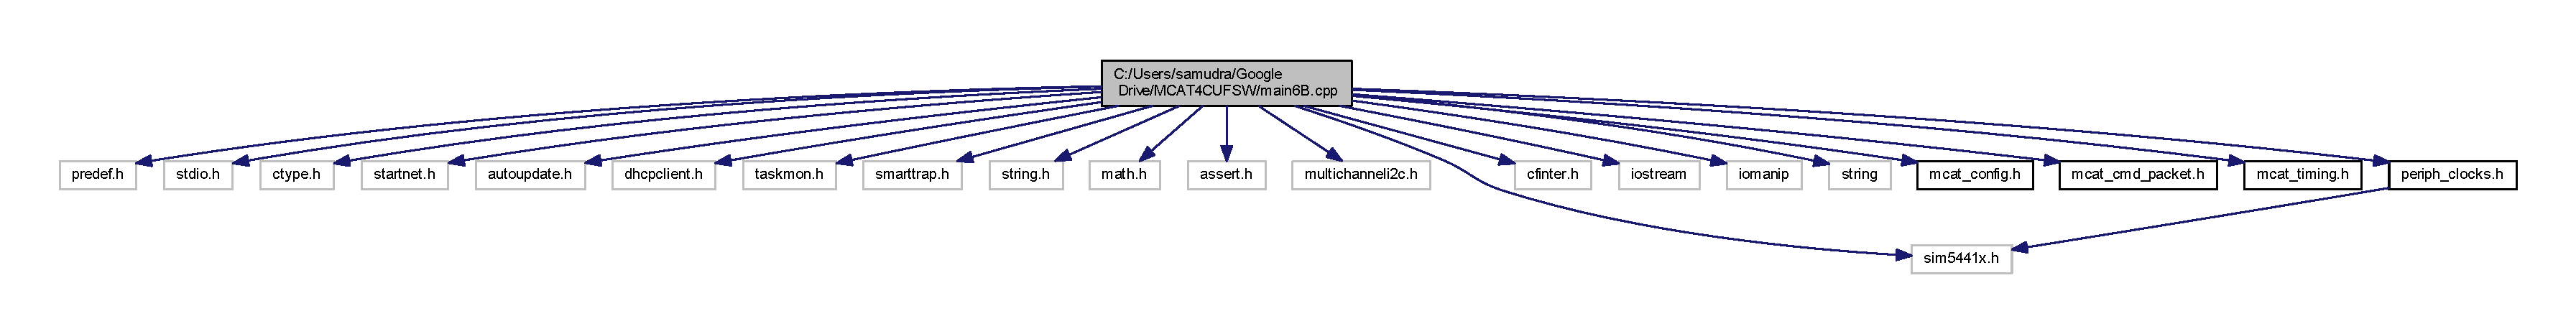
\includegraphics[width=350pt]{main6_b_8cpp__incl}
\end{center}
\end{figure}
\subsection*{Functions}
\begin{DoxyCompactItemize}
\item 
void \hyperlink{main6_b_8cpp_af3350bd69feae78ebcd4f766916eeb67}{parse\+C\+M\+D\+Packet} (char C\+M\+D\+Packet\mbox{[}I2\+C\+\_\+\+M\+A\+X\+\_\+\+B\+U\+F\+\_\+\+S\+I\+Z\+E\mbox{]})
\item 
void \hyperlink{main6_b_8cpp_aa3032893ba2f121a12d4cecf88277580}{parse\+Block\+G} (string Block\+G)
\item 
void \hyperlink{main6_b_8cpp_ab8ff54f4b027d2dfb6d3b63194fc15a4}{parse\+Block\+C\+U} (string Block\+C\+U)
\item 
void \hyperlink{main6_b_8cpp_a72e39dd7a2538b8b278f927ffd051bde}{parse\+Block\+I\+P\+D} (string Block\+I\+P\+D)
\item 
void \hyperlink{main6_b_8cpp_a8109658a433363943c469e7743c238ab}{parse\+Block\+P\+P\+U} (string Block\+P\+P\+U)
\item 
B\+Y\+T\+E \hyperlink{main6_b_8cpp_a22bb15ed96d4891d904b55838e451124}{Ascii2\+Byte} (char $\ast$buf)
\item 
void \hyperlink{main6_b_8cpp_ad16e5e62f3579a7048e6b981b172885e}{menu} (void)
\item 
void \hyperlink{main6_b_8cpp_ace7b2f4c33cbf41f3a43c7be01ff7aec}{User\+Main} (void $\ast$pd)
\item 
void \hyperlink{main6_b_8cpp_a486c7b37eb37847afaeeb6c73de398b9}{display\+Config} ()
\item 
void \hyperlink{main6_b_8cpp_a11ee600b69b27b0bb2d1b5b6e8ece140}{stop\+Pulses} (void $\ast$pdata)
\item 
void \hyperlink{main6_b_8cpp_a10570e6420ce0f0a076e1e9d3518d305}{init\+D\+M\+A\+T\+I\+M\+E\+R1} ()
\item 
void \hyperlink{main6_b_8cpp_a7c3f73193878c079945a21075f128059}{Set\+Intc} (long func, int vector, int level, int prio)
\item 
void \hyperlink{main6_b_8cpp_a8a64466bfb43094b3aec845670b959b4}{set\+Defaults} ()
\item 
void \hyperlink{main6_b_8cpp_a238885c747f586049b766fa4fcd5ec12}{disable\+All} ()
\item 
void \hyperlink{main6_b_8cpp_af2e78c1a970cd9490fcc3a5ac8015e6b}{debug\+Print} (string debug\+Msg)
\item 
\hyperlink{main6_b_8cpp_a89200d64c07024287b4ef31901f44e15}{I\+N\+T\+E\+R\+R\+U\+P\+T} (func\+\_\+isr, 0x2600)
\item 
void \hyperlink{main6_b_8cpp_acbfa28dfc2a41cc9cea58425f9b75178}{control\+P\+M\+A} (B\+O\+O\+L P\+M\+Flag)
\item 
void \hyperlink{main6_b_8cpp_ae4e046c7843050c83a5f70092acdbe1d}{control18\+L} (int requested\+Channel, int L\+Flag)
\item 
void \hyperlink{main6_b_8cpp_a2f5a551d47d5257bf34046aede82024e}{control18\+Hmanual} (int requested\+Channel, int H\+Flag)
\item 
void \hyperlink{main6_b_8cpp_a92a0eb6ae19d1612e39cbf1fd318d406}{set\+T\+P1} (long Frequency)
\item 
void \hyperlink{main6_b_8cpp_a8f5495a6630209795a3fbd7fa61a18e8}{control\+T\+P1} (B\+O\+O\+L T\+P1\+Flag)
\item 
void \hyperlink{main6_b_8cpp_a0ecec396fb6600a2f4897e7f30318159}{go\+F\+I\+R} ()
\item 
void \hyperlink{main6_b_8cpp_a2d0df7e0313c78e94bb4fafbc5752d67}{go\+F\+I\+Rfrom\+R\+U\+N} ()
\item 
void \hyperlink{main6_b_8cpp_ae0014243028b5cd808de963c18d01b11}{go\+F\+I\+Rfrom\+S\+B\+Y} ()
\item 
void \hyperlink{main6_b_8cpp_affc7dbdeb188c8169ccc6478143538d6}{go\+F\+I\+Rfrom\+I\+D\+L} ()
\item 
void \hyperlink{main6_b_8cpp_af57dea23daabb0f6e6d27f2ef21c9a54}{go\+R\+U\+N} ()
\item 
void \hyperlink{main6_b_8cpp_a6d712eb455e679cbf844c6742e7be6a0}{go\+R\+U\+Nfrom\+F\+I\+R} ()
\item 
void \hyperlink{main6_b_8cpp_a4770c1a01b1be1b23772d600b787d411}{go\+R\+U\+Nfrom\+S\+B\+Y} ()
\item 
void \hyperlink{main6_b_8cpp_a300391508ed006e4cd4ee0f9f316f3b4}{go\+R\+U\+Nfrom\+I\+D\+L} ()
\item 
void \hyperlink{main6_b_8cpp_a646dbe8155e1ee44efac5d50a7de878e}{go\+S\+B\+Y} ()
\item 
void \hyperlink{main6_b_8cpp_ae0ed43b60101aed3be6bea960293275d}{go\+S\+B\+Yfrom\+F\+I\+R} ()
\item 
void \hyperlink{main6_b_8cpp_a2d0b911e7b667c6a18000005acb28777}{go\+S\+B\+Yfrom\+R\+U\+N} ()
\item 
void \hyperlink{main6_b_8cpp_a37a57a2b0feb89b22b270931ae440c35}{go\+S\+B\+Yfrom\+I\+D\+L} ()
\item 
void \hyperlink{main6_b_8cpp_aa8d8f1cf694be5de1ac89b91627c0f51}{go\+I\+D\+L} ()
\item 
void \hyperlink{main6_b_8cpp_a3e3cc85ab7a91d6808984a0f78a5f9f8}{go\+I\+D\+Lfrom\+S\+B\+Y} ()
\item 
void \hyperlink{main6_b_8cpp_a690d16feac877ce7000b00e151dffd82}{go\+I\+D\+Lfrom\+R\+U\+N} ()
\item 
void \hyperlink{main6_b_8cpp_ae5438692f2a6c279129ecc19a91568f2}{go\+I\+D\+Lfrom\+F\+I\+R} ()
\item 
void \hyperlink{main6_b_8cpp_a9b07c4b395adfe387d12241e7ebaaae6}{set\+New\+Mode} (string cmd\+Mode\+Request, string \hyperlink{main6_c_8cpp_ab996ab5995af95792f5af3586d943d58}{cmd\+Mode\+Current})
\item 
void \hyperlink{main6_b_8cpp_a5b251dff1da28eda51e8b51bc4b2baf7}{do\+Setup\+I\+O} ()
\end{DoxyCompactItemize}
\subsection*{Variables}
\begin{DoxyCompactItemize}
\item 
char \hyperlink{main6_b_8cpp_a7f7c6b9d49f7b1a42e631ec964d939b9}{id\+C\+U} \mbox{[}80\mbox{]}
\item 
string \hyperlink{main6_b_8cpp_a405cdd34a0ec61abf8c5205c7a8c3182}{cmd\+Version} =\char`\"{}\char`\"{}
\item 
string \hyperlink{main6_b_8cpp_a8a9767341d04352fccd7068bc1d7c370}{cmd\+Mode} =\char`\"{}\char`\"{}
\item 
string \hyperlink{main6_b_8cpp_ab996ab5995af95792f5af3586d943d58}{cmd\+Mode\+Current} =\char`\"{}\char`\"{}
\item 
string \hyperlink{main6_b_8cpp_ad9049cc701250fb177b8e99713039762}{s\+\_\+freq\+T\+P1} =\char`\"{}\char`\"{}
\item 
string \hyperlink{main6_b_8cpp_a396dd1e7a6a9a4dc8b908980e2e1ded4}{s\+\_\+freq\+T\+P2} =\char`\"{}\char`\"{}
\item 
string \hyperlink{main6_b_8cpp_a62d24bc7666ac0bb0d8728dba649a256}{s\+\_\+freq\+T\+P3} =\char`\"{}\char`\"{}
\item 
string \hyperlink{main6_b_8cpp_a6a2b49919f4f32a4af53700ed1cde8ed}{s\+\_\+freq\+T\+P4} =\char`\"{}\char`\"{}
\item 
string \hyperlink{main6_b_8cpp_a4ba85625fa845776a2d64a3f58f36c42}{s\+\_\+count\+Ch1} =\char`\"{}\char`\"{}
\item 
string \hyperlink{main6_b_8cpp_a88730d26d9b63cdf8e4ca277a76b638d}{s\+\_\+count\+Ch2} =\char`\"{}\char`\"{}
\item 
string \hyperlink{main6_b_8cpp_a09052171565a4f15cbfdbc2ebcdd3fff}{s\+\_\+count\+Ch3} =\char`\"{}\char`\"{}
\item 
string \hyperlink{main6_b_8cpp_a32bb7a1f63c92a94ec3d098853bd883b}{s\+\_\+count\+Ch4} =\char`\"{}\char`\"{}
\item 
long \hyperlink{main6_b_8cpp_a7d2353ca53d5b5b259a823a92b7b519e}{freq\+T\+P1} = 10
\item 
long \hyperlink{main6_b_8cpp_a511164d7a4515d9a1f07ccfbda7ea294}{freq\+T\+P2} = 10
\item 
long \hyperlink{main6_b_8cpp_afae1443270cbb13745f612d5425f94a7}{freq\+T\+P3} = 10
\item 
long \hyperlink{main6_b_8cpp_a7cc56f796c77e7b30948d992bacc0429}{freq\+T\+P4} = 10
\item 
long \hyperlink{main6_b_8cpp_a9a1f402dd7e47f25ca3aa9ae7a8d0dc6}{count\+Ch1} = 0
\item 
long \hyperlink{main6_b_8cpp_a49801da896cbdab7c4b39b8e012c1a18}{count\+Ch2} = 0
\item 
long \hyperlink{main6_b_8cpp_a0582794ca95bdcf8787638b7def0177c}{count\+Ch3} = 0
\item 
long \hyperlink{main6_b_8cpp_a1de46864f078711d257187f01dfff541}{count\+Ch4} = 0
\item 
string \hyperlink{main6_b_8cpp_a37ec136ae86c4b7dc81f393bb1a01af7}{s\+\_\+cmd\+P18\+H1} =\char`\"{}\char`\"{}
\item 
string \hyperlink{main6_b_8cpp_a46ce373f60085f5900464cd0731fa20e}{s\+\_\+cmd\+P18\+H2} =\char`\"{}\char`\"{}
\item 
string \hyperlink{main6_b_8cpp_a909acdc96889fb5885793e8bc70b083e}{s\+\_\+cmd\+P18\+H3} =\char`\"{}\char`\"{}
\item 
string \hyperlink{main6_b_8cpp_a607e82175ad61b864bfa84e686437947}{s\+\_\+cmd\+P18\+H4} =\char`\"{}\char`\"{}
\item 
bool \hyperlink{main6_b_8cpp_a1a10d6a42e7c3ba1ad7f396b687a7eb7}{cmd\+P18\+H1}
\item 
bool \hyperlink{main6_b_8cpp_a03df8cc8ee6b4d7ba8a3d2ad50914508}{cmd\+P18\+H2}
\item 
bool \hyperlink{main6_b_8cpp_aba803fecbea259c5af71f0b9f2e9fa5a}{cmd\+P18\+H3}
\item 
bool \hyperlink{main6_b_8cpp_a74d16dd0ede9be1a1645027bd2e6fb21}{cmd\+P18\+H4}
\item 
B\+Y\+T\+E \hyperlink{main6_b_8cpp_a750abfb0120c1735c922980bd47640a5}{buffer} \mbox{[}I2\+C\+\_\+\+M\+A\+X\+\_\+\+B\+U\+F\+\_\+\+S\+I\+Z\+E\mbox{]}
\item 
char \hyperlink{main6_b_8cpp_af54d77a991da4ba360d594c2589140df}{I2\+C\+Input\+Buffer} \mbox{[}I2\+C\+\_\+\+M\+A\+X\+\_\+\+B\+U\+F\+\_\+\+S\+I\+Z\+E\mbox{]}
\item 
char $\ast$ \hyperlink{main6_b_8cpp_abed0c40696905e144ed4118061acf700}{inbuf} = \hyperlink{_v2_01main_8cpp_af54d77a991da4ba360d594c2589140df}{I2\+C\+Input\+Buffer}
\item 
B\+Y\+T\+E \hyperlink{main6_b_8cpp_a92fb5ea5b6a7d108dea33dd07809152d}{address} = \hyperlink{mcatsubsystemconfig_8h_a8fe248bd745b90e2bfe94d8c5fce0a53}{C\+U\+\_\+\+I2\+C\+\_\+\+S\+L\+A\+V\+E\+\_\+\+A\+D\+D\+R}
\item 
B\+Y\+T\+E \hyperlink{main6_b_8cpp_a6c3dedd37414833dd07e72ee4a642d13}{I2\+C\+Stat}
\end{DoxyCompactItemize}


\subsection{Function Documentation}
\hypertarget{main6_b_8cpp_a22bb15ed96d4891d904b55838e451124}{}\index{main6\+B.\+cpp@{main6\+B.\+cpp}!Ascii2\+Byte@{Ascii2\+Byte}}
\index{Ascii2\+Byte@{Ascii2\+Byte}!main6\+B.\+cpp@{main6\+B.\+cpp}}
\subsubsection[{Ascii2\+Byte}]{\setlength{\rightskip}{0pt plus 5cm}B\+Y\+T\+E Ascii2\+Byte (
\begin{DoxyParamCaption}
\item[{char $\ast$}]{buf}
\end{DoxyParamCaption}
)}\label{main6_b_8cpp_a22bb15ed96d4891d904b55838e451124}


Definition at line 1175 of file main6\+B.\+cpp.

\hypertarget{main6_b_8cpp_a2f5a551d47d5257bf34046aede82024e}{}\index{main6\+B.\+cpp@{main6\+B.\+cpp}!control18\+Hmanual@{control18\+Hmanual}}
\index{control18\+Hmanual@{control18\+Hmanual}!main6\+B.\+cpp@{main6\+B.\+cpp}}
\subsubsection[{control18\+Hmanual}]{\setlength{\rightskip}{0pt plus 5cm}void control18\+Hmanual (
\begin{DoxyParamCaption}
\item[{int}]{requested\+Channel, }
\item[{int}]{H\+Flag}
\end{DoxyParamCaption}
)}\label{main6_b_8cpp_a2f5a551d47d5257bf34046aede82024e}


Definition at line 368 of file main6\+B.\+cpp.

\hypertarget{main6_b_8cpp_ae4e046c7843050c83a5f70092acdbe1d}{}\index{main6\+B.\+cpp@{main6\+B.\+cpp}!control18\+L@{control18\+L}}
\index{control18\+L@{control18\+L}!main6\+B.\+cpp@{main6\+B.\+cpp}}
\subsubsection[{control18\+L}]{\setlength{\rightskip}{0pt plus 5cm}void control18\+L (
\begin{DoxyParamCaption}
\item[{int}]{requested\+Channel, }
\item[{int}]{L\+Flag}
\end{DoxyParamCaption}
)}\label{main6_b_8cpp_ae4e046c7843050c83a5f70092acdbe1d}


Definition at line 246 of file main6\+B.\+cpp.

\hypertarget{main6_b_8cpp_acbfa28dfc2a41cc9cea58425f9b75178}{}\index{main6\+B.\+cpp@{main6\+B.\+cpp}!control\+P\+M\+A@{control\+P\+M\+A}}
\index{control\+P\+M\+A@{control\+P\+M\+A}!main6\+B.\+cpp@{main6\+B.\+cpp}}
\subsubsection[{control\+P\+M\+A}]{\setlength{\rightskip}{0pt plus 5cm}void control\+P\+M\+A (
\begin{DoxyParamCaption}
\item[{B\+O\+O\+L}]{P\+M\+Flag}
\end{DoxyParamCaption}
)}\label{main6_b_8cpp_acbfa28dfc2a41cc9cea58425f9b75178}


Definition at line 229 of file main6\+B.\+cpp.

\hypertarget{main6_b_8cpp_a8f5495a6630209795a3fbd7fa61a18e8}{}\index{main6\+B.\+cpp@{main6\+B.\+cpp}!control\+T\+P1@{control\+T\+P1}}
\index{control\+T\+P1@{control\+T\+P1}!main6\+B.\+cpp@{main6\+B.\+cpp}}
\subsubsection[{control\+T\+P1}]{\setlength{\rightskip}{0pt plus 5cm}void control\+T\+P1 (
\begin{DoxyParamCaption}
\item[{B\+O\+O\+L}]{T\+P1\+Flag}
\end{DoxyParamCaption}
)}\label{main6_b_8cpp_a8f5495a6630209795a3fbd7fa61a18e8}
from 5270 code set /// D\+O N\+O\+T U\+S\+E Set\+Intc((long) \&func\+\_\+isr, 19, 1, 1); 

Definition at line 560 of file main6\+B.\+cpp.

\hypertarget{main6_b_8cpp_af2e78c1a970cd9490fcc3a5ac8015e6b}{}\index{main6\+B.\+cpp@{main6\+B.\+cpp}!debug\+Print@{debug\+Print}}
\index{debug\+Print@{debug\+Print}!main6\+B.\+cpp@{main6\+B.\+cpp}}
\subsubsection[{debug\+Print}]{\setlength{\rightskip}{0pt plus 5cm}void debug\+Print (
\begin{DoxyParamCaption}
\item[{string}]{debug\+Msg}
\end{DoxyParamCaption}
)}\label{main6_b_8cpp_af2e78c1a970cd9490fcc3a5ac8015e6b}


Definition at line 154 of file main6\+B.\+cpp.

\hypertarget{main6_b_8cpp_a238885c747f586049b766fa4fcd5ec12}{}\index{main6\+B.\+cpp@{main6\+B.\+cpp}!disable\+All@{disable\+All}}
\index{disable\+All@{disable\+All}!main6\+B.\+cpp@{main6\+B.\+cpp}}
\subsubsection[{disable\+All}]{\setlength{\rightskip}{0pt plus 5cm}void disable\+All (
\begin{DoxyParamCaption}
{}
\end{DoxyParamCaption}
)}\label{main6_b_8cpp_a238885c747f586049b766fa4fcd5ec12}


Definition at line 772 of file main6\+B.\+cpp.

\hypertarget{main6_b_8cpp_a486c7b37eb37847afaeeb6c73de398b9}{}\index{main6\+B.\+cpp@{main6\+B.\+cpp}!display\+Config@{display\+Config}}
\index{display\+Config@{display\+Config}!main6\+B.\+cpp@{main6\+B.\+cpp}}
\subsubsection[{display\+Config}]{\setlength{\rightskip}{0pt plus 5cm}void display\+Config (
\begin{DoxyParamCaption}
{}
\end{DoxyParamCaption}
)}\label{main6_b_8cpp_a486c7b37eb37847afaeeb6c73de398b9}
\hypertarget{main6_b_8cpp_a5b251dff1da28eda51e8b51bc4b2baf7}{}\index{main6\+B.\+cpp@{main6\+B.\+cpp}!do\+Setup\+I\+O@{do\+Setup\+I\+O}}
\index{do\+Setup\+I\+O@{do\+Setup\+I\+O}!main6\+B.\+cpp@{main6\+B.\+cpp}}
\subsubsection[{do\+Setup\+I\+O}]{\setlength{\rightskip}{0pt plus 5cm}void do\+Setup\+I\+O (
\begin{DoxyParamCaption}
{}
\end{DoxyParamCaption}
)}\label{main6_b_8cpp_a5b251dff1da28eda51e8b51bc4b2baf7}


Definition at line 833 of file main6\+B.\+cpp.

\hypertarget{main6_b_8cpp_a0ecec396fb6600a2f4897e7f30318159}{}\index{main6\+B.\+cpp@{main6\+B.\+cpp}!go\+F\+I\+R@{go\+F\+I\+R}}
\index{go\+F\+I\+R@{go\+F\+I\+R}!main6\+B.\+cpp@{main6\+B.\+cpp}}
\subsubsection[{go\+F\+I\+R}]{\setlength{\rightskip}{0pt plus 5cm}void go\+F\+I\+R (
\begin{DoxyParamCaption}
{}
\end{DoxyParamCaption}
)}\label{main6_b_8cpp_a0ecec396fb6600a2f4897e7f30318159}


Definition at line 594 of file main6\+B.\+cpp.

\hypertarget{main6_b_8cpp_affc7dbdeb188c8169ccc6478143538d6}{}\index{main6\+B.\+cpp@{main6\+B.\+cpp}!go\+F\+I\+Rfrom\+I\+D\+L@{go\+F\+I\+Rfrom\+I\+D\+L}}
\index{go\+F\+I\+Rfrom\+I\+D\+L@{go\+F\+I\+Rfrom\+I\+D\+L}!main6\+B.\+cpp@{main6\+B.\+cpp}}
\subsubsection[{go\+F\+I\+Rfrom\+I\+D\+L}]{\setlength{\rightskip}{0pt plus 5cm}void go\+F\+I\+Rfrom\+I\+D\+L (
\begin{DoxyParamCaption}
{}
\end{DoxyParamCaption}
)}\label{main6_b_8cpp_affc7dbdeb188c8169ccc6478143538d6}


Definition at line 628 of file main6\+B.\+cpp.

\hypertarget{main6_b_8cpp_a2d0df7e0313c78e94bb4fafbc5752d67}{}\index{main6\+B.\+cpp@{main6\+B.\+cpp}!go\+F\+I\+Rfrom\+R\+U\+N@{go\+F\+I\+Rfrom\+R\+U\+N}}
\index{go\+F\+I\+Rfrom\+R\+U\+N@{go\+F\+I\+Rfrom\+R\+U\+N}!main6\+B.\+cpp@{main6\+B.\+cpp}}
\subsubsection[{go\+F\+I\+Rfrom\+R\+U\+N}]{\setlength{\rightskip}{0pt plus 5cm}void go\+F\+I\+Rfrom\+R\+U\+N (
\begin{DoxyParamCaption}
{}
\end{DoxyParamCaption}
)}\label{main6_b_8cpp_a2d0df7e0313c78e94bb4fafbc5752d67}


Definition at line 599 of file main6\+B.\+cpp.

\hypertarget{main6_b_8cpp_ae0014243028b5cd808de963c18d01b11}{}\index{main6\+B.\+cpp@{main6\+B.\+cpp}!go\+F\+I\+Rfrom\+S\+B\+Y@{go\+F\+I\+Rfrom\+S\+B\+Y}}
\index{go\+F\+I\+Rfrom\+S\+B\+Y@{go\+F\+I\+Rfrom\+S\+B\+Y}!main6\+B.\+cpp@{main6\+B.\+cpp}}
\subsubsection[{go\+F\+I\+Rfrom\+S\+B\+Y}]{\setlength{\rightskip}{0pt plus 5cm}void go\+F\+I\+Rfrom\+S\+B\+Y (
\begin{DoxyParamCaption}
{}
\end{DoxyParamCaption}
)}\label{main6_b_8cpp_ae0014243028b5cd808de963c18d01b11}


Definition at line 624 of file main6\+B.\+cpp.

\hypertarget{main6_b_8cpp_aa8d8f1cf694be5de1ac89b91627c0f51}{}\index{main6\+B.\+cpp@{main6\+B.\+cpp}!go\+I\+D\+L@{go\+I\+D\+L}}
\index{go\+I\+D\+L@{go\+I\+D\+L}!main6\+B.\+cpp@{main6\+B.\+cpp}}
\subsubsection[{go\+I\+D\+L}]{\setlength{\rightskip}{0pt plus 5cm}void go\+I\+D\+L (
\begin{DoxyParamCaption}
{}
\end{DoxyParamCaption}
)}\label{main6_b_8cpp_aa8d8f1cf694be5de1ac89b91627c0f51}


Definition at line 675 of file main6\+B.\+cpp.

\hypertarget{main6_b_8cpp_ae5438692f2a6c279129ecc19a91568f2}{}\index{main6\+B.\+cpp@{main6\+B.\+cpp}!go\+I\+D\+Lfrom\+F\+I\+R@{go\+I\+D\+Lfrom\+F\+I\+R}}
\index{go\+I\+D\+Lfrom\+F\+I\+R@{go\+I\+D\+Lfrom\+F\+I\+R}!main6\+B.\+cpp@{main6\+B.\+cpp}}
\subsubsection[{go\+I\+D\+Lfrom\+F\+I\+R}]{\setlength{\rightskip}{0pt plus 5cm}void go\+I\+D\+Lfrom\+F\+I\+R (
\begin{DoxyParamCaption}
{}
\end{DoxyParamCaption}
)}\label{main6_b_8cpp_ae5438692f2a6c279129ecc19a91568f2}


Definition at line 688 of file main6\+B.\+cpp.

\hypertarget{main6_b_8cpp_a690d16feac877ce7000b00e151dffd82}{}\index{main6\+B.\+cpp@{main6\+B.\+cpp}!go\+I\+D\+Lfrom\+R\+U\+N@{go\+I\+D\+Lfrom\+R\+U\+N}}
\index{go\+I\+D\+Lfrom\+R\+U\+N@{go\+I\+D\+Lfrom\+R\+U\+N}!main6\+B.\+cpp@{main6\+B.\+cpp}}
\subsubsection[{go\+I\+D\+Lfrom\+R\+U\+N}]{\setlength{\rightskip}{0pt plus 5cm}void go\+I\+D\+Lfrom\+R\+U\+N (
\begin{DoxyParamCaption}
{}
\end{DoxyParamCaption}
)}\label{main6_b_8cpp_a690d16feac877ce7000b00e151dffd82}


Definition at line 684 of file main6\+B.\+cpp.

\hypertarget{main6_b_8cpp_a3e3cc85ab7a91d6808984a0f78a5f9f8}{}\index{main6\+B.\+cpp@{main6\+B.\+cpp}!go\+I\+D\+Lfrom\+S\+B\+Y@{go\+I\+D\+Lfrom\+S\+B\+Y}}
\index{go\+I\+D\+Lfrom\+S\+B\+Y@{go\+I\+D\+Lfrom\+S\+B\+Y}!main6\+B.\+cpp@{main6\+B.\+cpp}}
\subsubsection[{go\+I\+D\+Lfrom\+S\+B\+Y}]{\setlength{\rightskip}{0pt plus 5cm}void go\+I\+D\+Lfrom\+S\+B\+Y (
\begin{DoxyParamCaption}
{}
\end{DoxyParamCaption}
)}\label{main6_b_8cpp_a3e3cc85ab7a91d6808984a0f78a5f9f8}


Definition at line 680 of file main6\+B.\+cpp.

\hypertarget{main6_b_8cpp_af57dea23daabb0f6e6d27f2ef21c9a54}{}\index{main6\+B.\+cpp@{main6\+B.\+cpp}!go\+R\+U\+N@{go\+R\+U\+N}}
\index{go\+R\+U\+N@{go\+R\+U\+N}!main6\+B.\+cpp@{main6\+B.\+cpp}}
\subsubsection[{go\+R\+U\+N}]{\setlength{\rightskip}{0pt plus 5cm}void go\+R\+U\+N (
\begin{DoxyParamCaption}
{}
\end{DoxyParamCaption}
)}\label{main6_b_8cpp_af57dea23daabb0f6e6d27f2ef21c9a54}


Definition at line 633 of file main6\+B.\+cpp.

\hypertarget{main6_b_8cpp_a6d712eb455e679cbf844c6742e7be6a0}{}\index{main6\+B.\+cpp@{main6\+B.\+cpp}!go\+R\+U\+Nfrom\+F\+I\+R@{go\+R\+U\+Nfrom\+F\+I\+R}}
\index{go\+R\+U\+Nfrom\+F\+I\+R@{go\+R\+U\+Nfrom\+F\+I\+R}!main6\+B.\+cpp@{main6\+B.\+cpp}}
\subsubsection[{go\+R\+U\+Nfrom\+F\+I\+R}]{\setlength{\rightskip}{0pt plus 5cm}void go\+R\+U\+Nfrom\+F\+I\+R (
\begin{DoxyParamCaption}
{}
\end{DoxyParamCaption}
)}\label{main6_b_8cpp_a6d712eb455e679cbf844c6742e7be6a0}


Definition at line 644 of file main6\+B.\+cpp.

\hypertarget{main6_b_8cpp_a300391508ed006e4cd4ee0f9f316f3b4}{}\index{main6\+B.\+cpp@{main6\+B.\+cpp}!go\+R\+U\+Nfrom\+I\+D\+L@{go\+R\+U\+Nfrom\+I\+D\+L}}
\index{go\+R\+U\+Nfrom\+I\+D\+L@{go\+R\+U\+Nfrom\+I\+D\+L}!main6\+B.\+cpp@{main6\+B.\+cpp}}
\subsubsection[{go\+R\+U\+Nfrom\+I\+D\+L}]{\setlength{\rightskip}{0pt plus 5cm}void go\+R\+U\+Nfrom\+I\+D\+L (
\begin{DoxyParamCaption}
{}
\end{DoxyParamCaption}
)}\label{main6_b_8cpp_a300391508ed006e4cd4ee0f9f316f3b4}


Definition at line 652 of file main6\+B.\+cpp.

\hypertarget{main6_b_8cpp_a4770c1a01b1be1b23772d600b787d411}{}\index{main6\+B.\+cpp@{main6\+B.\+cpp}!go\+R\+U\+Nfrom\+S\+B\+Y@{go\+R\+U\+Nfrom\+S\+B\+Y}}
\index{go\+R\+U\+Nfrom\+S\+B\+Y@{go\+R\+U\+Nfrom\+S\+B\+Y}!main6\+B.\+cpp@{main6\+B.\+cpp}}
\subsubsection[{go\+R\+U\+Nfrom\+S\+B\+Y}]{\setlength{\rightskip}{0pt plus 5cm}void go\+R\+U\+Nfrom\+S\+B\+Y (
\begin{DoxyParamCaption}
{}
\end{DoxyParamCaption}
)}\label{main6_b_8cpp_a4770c1a01b1be1b23772d600b787d411}


Definition at line 648 of file main6\+B.\+cpp.

\hypertarget{main6_b_8cpp_a646dbe8155e1ee44efac5d50a7de878e}{}\index{main6\+B.\+cpp@{main6\+B.\+cpp}!go\+S\+B\+Y@{go\+S\+B\+Y}}
\index{go\+S\+B\+Y@{go\+S\+B\+Y}!main6\+B.\+cpp@{main6\+B.\+cpp}}
\subsubsection[{go\+S\+B\+Y}]{\setlength{\rightskip}{0pt plus 5cm}void go\+S\+B\+Y (
\begin{DoxyParamCaption}
{}
\end{DoxyParamCaption}
)}\label{main6_b_8cpp_a646dbe8155e1ee44efac5d50a7de878e}


Definition at line 657 of file main6\+B.\+cpp.

\hypertarget{main6_b_8cpp_ae0ed43b60101aed3be6bea960293275d}{}\index{main6\+B.\+cpp@{main6\+B.\+cpp}!go\+S\+B\+Yfrom\+F\+I\+R@{go\+S\+B\+Yfrom\+F\+I\+R}}
\index{go\+S\+B\+Yfrom\+F\+I\+R@{go\+S\+B\+Yfrom\+F\+I\+R}!main6\+B.\+cpp@{main6\+B.\+cpp}}
\subsubsection[{go\+S\+B\+Yfrom\+F\+I\+R}]{\setlength{\rightskip}{0pt plus 5cm}void go\+S\+B\+Yfrom\+F\+I\+R (
\begin{DoxyParamCaption}
{}
\end{DoxyParamCaption}
)}\label{main6_b_8cpp_ae0ed43b60101aed3be6bea960293275d}


Definition at line 662 of file main6\+B.\+cpp.

\hypertarget{main6_b_8cpp_a37a57a2b0feb89b22b270931ae440c35}{}\index{main6\+B.\+cpp@{main6\+B.\+cpp}!go\+S\+B\+Yfrom\+I\+D\+L@{go\+S\+B\+Yfrom\+I\+D\+L}}
\index{go\+S\+B\+Yfrom\+I\+D\+L@{go\+S\+B\+Yfrom\+I\+D\+L}!main6\+B.\+cpp@{main6\+B.\+cpp}}
\subsubsection[{go\+S\+B\+Yfrom\+I\+D\+L}]{\setlength{\rightskip}{0pt plus 5cm}void go\+S\+B\+Yfrom\+I\+D\+L (
\begin{DoxyParamCaption}
{}
\end{DoxyParamCaption}
)}\label{main6_b_8cpp_a37a57a2b0feb89b22b270931ae440c35}


Definition at line 670 of file main6\+B.\+cpp.

\hypertarget{main6_b_8cpp_a2d0b911e7b667c6a18000005acb28777}{}\index{main6\+B.\+cpp@{main6\+B.\+cpp}!go\+S\+B\+Yfrom\+R\+U\+N@{go\+S\+B\+Yfrom\+R\+U\+N}}
\index{go\+S\+B\+Yfrom\+R\+U\+N@{go\+S\+B\+Yfrom\+R\+U\+N}!main6\+B.\+cpp@{main6\+B.\+cpp}}
\subsubsection[{go\+S\+B\+Yfrom\+R\+U\+N}]{\setlength{\rightskip}{0pt plus 5cm}void go\+S\+B\+Yfrom\+R\+U\+N (
\begin{DoxyParamCaption}
{}
\end{DoxyParamCaption}
)}\label{main6_b_8cpp_a2d0b911e7b667c6a18000005acb28777}


Definition at line 666 of file main6\+B.\+cpp.

\hypertarget{main6_b_8cpp_a10570e6420ce0f0a076e1e9d3518d305}{}\index{main6\+B.\+cpp@{main6\+B.\+cpp}!init\+D\+M\+A\+T\+I\+M\+E\+R1@{init\+D\+M\+A\+T\+I\+M\+E\+R1}}
\index{init\+D\+M\+A\+T\+I\+M\+E\+R1@{init\+D\+M\+A\+T\+I\+M\+E\+R1}!main6\+B.\+cpp@{main6\+B.\+cpp}}
\subsubsection[{init\+D\+M\+A\+T\+I\+M\+E\+R1}]{\setlength{\rightskip}{0pt plus 5cm}void init\+D\+M\+A\+T\+I\+M\+E\+R1 (
\begin{DoxyParamCaption}
{}
\end{DoxyParamCaption}
)}\label{main6_b_8cpp_a10570e6420ce0f0a076e1e9d3518d305}
from 5270 code set /// D\+O N\+O\+T U\+S\+E Set\+Intc((long) \&func\+\_\+isr, 19, 1, 1); 

Definition at line 818 of file main6\+B.\+cpp.

\hypertarget{main6_b_8cpp_a89200d64c07024287b4ef31901f44e15}{}\index{main6\+B.\+cpp@{main6\+B.\+cpp}!I\+N\+T\+E\+R\+R\+U\+P\+T@{I\+N\+T\+E\+R\+R\+U\+P\+T}}
\index{I\+N\+T\+E\+R\+R\+U\+P\+T@{I\+N\+T\+E\+R\+R\+U\+P\+T}!main6\+B.\+cpp@{main6\+B.\+cpp}}
\subsubsection[{I\+N\+T\+E\+R\+R\+U\+P\+T}]{\setlength{\rightskip}{0pt plus 5cm}I\+N\+T\+E\+R\+R\+U\+P\+T (
\begin{DoxyParamCaption}
\item[{func\+\_\+isr}]{, }
\item[{0x2600}]{}
\end{DoxyParamCaption}
)}\label{main6_b_8cpp_a89200d64c07024287b4ef31901f44e15}


Definition at line 162 of file main6\+B.\+cpp.

\hypertarget{main6_b_8cpp_ad16e5e62f3579a7048e6b981b172885e}{}\index{main6\+B.\+cpp@{main6\+B.\+cpp}!menu@{menu}}
\index{menu@{menu}!main6\+B.\+cpp@{main6\+B.\+cpp}}
\subsubsection[{menu}]{\setlength{\rightskip}{0pt plus 5cm}void menu (
\begin{DoxyParamCaption}
\item[{void}]{}
\end{DoxyParamCaption}
)}\label{main6_b_8cpp_ad16e5e62f3579a7048e6b981b172885e}


Definition at line 1193 of file main6\+B.\+cpp.

\hypertarget{main6_b_8cpp_ab8ff54f4b027d2dfb6d3b63194fc15a4}{}\index{main6\+B.\+cpp@{main6\+B.\+cpp}!parse\+Block\+C\+U@{parse\+Block\+C\+U}}
\index{parse\+Block\+C\+U@{parse\+Block\+C\+U}!main6\+B.\+cpp@{main6\+B.\+cpp}}
\subsubsection[{parse\+Block\+C\+U}]{\setlength{\rightskip}{0pt plus 5cm}void parse\+Block\+C\+U (
\begin{DoxyParamCaption}
\item[{string}]{Block\+C\+U}
\end{DoxyParamCaption}
)}\label{main6_b_8cpp_ab8ff54f4b027d2dfb6d3b63194fc15a4}


Definition at line 1049 of file main6\+B.\+cpp.

\hypertarget{main6_b_8cpp_aa3032893ba2f121a12d4cecf88277580}{}\index{main6\+B.\+cpp@{main6\+B.\+cpp}!parse\+Block\+G@{parse\+Block\+G}}
\index{parse\+Block\+G@{parse\+Block\+G}!main6\+B.\+cpp@{main6\+B.\+cpp}}
\subsubsection[{parse\+Block\+G}]{\setlength{\rightskip}{0pt plus 5cm}void parse\+Block\+G (
\begin{DoxyParamCaption}
\item[{string}]{Block\+G}
\end{DoxyParamCaption}
)}\label{main6_b_8cpp_aa3032893ba2f121a12d4cecf88277580}


Definition at line 1039 of file main6\+B.\+cpp.

\hypertarget{main6_b_8cpp_a72e39dd7a2538b8b278f927ffd051bde}{}\index{main6\+B.\+cpp@{main6\+B.\+cpp}!parse\+Block\+I\+P\+D@{parse\+Block\+I\+P\+D}}
\index{parse\+Block\+I\+P\+D@{parse\+Block\+I\+P\+D}!main6\+B.\+cpp@{main6\+B.\+cpp}}
\subsubsection[{parse\+Block\+I\+P\+D}]{\setlength{\rightskip}{0pt plus 5cm}void parse\+Block\+I\+P\+D (
\begin{DoxyParamCaption}
\item[{string}]{Block\+I\+P\+D}
\end{DoxyParamCaption}
)}\label{main6_b_8cpp_a72e39dd7a2538b8b278f927ffd051bde}


Definition at line 1060 of file main6\+B.\+cpp.

\hypertarget{main6_b_8cpp_a8109658a433363943c469e7743c238ab}{}\index{main6\+B.\+cpp@{main6\+B.\+cpp}!parse\+Block\+P\+P\+U@{parse\+Block\+P\+P\+U}}
\index{parse\+Block\+P\+P\+U@{parse\+Block\+P\+P\+U}!main6\+B.\+cpp@{main6\+B.\+cpp}}
\subsubsection[{parse\+Block\+P\+P\+U}]{\setlength{\rightskip}{0pt plus 5cm}void parse\+Block\+P\+P\+U (
\begin{DoxyParamCaption}
\item[{string}]{Block\+P\+P\+U}
\end{DoxyParamCaption}
)}\label{main6_b_8cpp_a8109658a433363943c469e7743c238ab}


Definition at line 1115 of file main6\+B.\+cpp.

\hypertarget{main6_b_8cpp_af3350bd69feae78ebcd4f766916eeb67}{}\index{main6\+B.\+cpp@{main6\+B.\+cpp}!parse\+C\+M\+D\+Packet@{parse\+C\+M\+D\+Packet}}
\index{parse\+C\+M\+D\+Packet@{parse\+C\+M\+D\+Packet}!main6\+B.\+cpp@{main6\+B.\+cpp}}
\subsubsection[{parse\+C\+M\+D\+Packet}]{\setlength{\rightskip}{0pt plus 5cm}void parse\+C\+M\+D\+Packet (
\begin{DoxyParamCaption}
\item[{char}]{C\+M\+D\+Packet\mbox{[}\+I2\+C\+\_\+\+M\+A\+X\+\_\+\+B\+U\+F\+\_\+\+S\+I\+Z\+E\mbox{]}}
\end{DoxyParamCaption}
)}\label{main6_b_8cpp_af3350bd69feae78ebcd4f766916eeb67}


Definition at line 894 of file main6\+B.\+cpp.

\hypertarget{main6_b_8cpp_a8a64466bfb43094b3aec845670b959b4}{}\index{main6\+B.\+cpp@{main6\+B.\+cpp}!set\+Defaults@{set\+Defaults}}
\index{set\+Defaults@{set\+Defaults}!main6\+B.\+cpp@{main6\+B.\+cpp}}
\subsubsection[{set\+Defaults}]{\setlength{\rightskip}{0pt plus 5cm}void set\+Defaults (
\begin{DoxyParamCaption}
{}
\end{DoxyParamCaption}
)}\label{main6_b_8cpp_a8a64466bfb43094b3aec845670b959b4}


Definition at line 779 of file main6\+B.\+cpp.

\hypertarget{main6_b_8cpp_a7c3f73193878c079945a21075f128059}{}\index{main6\+B.\+cpp@{main6\+B.\+cpp}!Set\+Intc@{Set\+Intc}}
\index{Set\+Intc@{Set\+Intc}!main6\+B.\+cpp@{main6\+B.\+cpp}}
\subsubsection[{Set\+Intc}]{\setlength{\rightskip}{0pt plus 5cm}void Set\+Intc (
\begin{DoxyParamCaption}
\item[{long}]{func, }
\item[{int}]{vector, }
\item[{int}]{level, }
\item[{int}]{prio}
\end{DoxyParamCaption}
)}\label{main6_b_8cpp_a7c3f73193878c079945a21075f128059}
\hypertarget{main6_b_8cpp_a9b07c4b395adfe387d12241e7ebaaae6}{}\index{main6\+B.\+cpp@{main6\+B.\+cpp}!set\+New\+Mode@{set\+New\+Mode}}
\index{set\+New\+Mode@{set\+New\+Mode}!main6\+B.\+cpp@{main6\+B.\+cpp}}
\subsubsection[{set\+New\+Mode}]{\setlength{\rightskip}{0pt plus 5cm}void set\+New\+Mode (
\begin{DoxyParamCaption}
\item[{string}]{cmd\+Mode\+Request, }
\item[{string}]{cmd\+Mode\+Current}
\end{DoxyParamCaption}
)}\label{main6_b_8cpp_a9b07c4b395adfe387d12241e7ebaaae6}


Definition at line 695 of file main6\+B.\+cpp.

\hypertarget{main6_b_8cpp_a92a0eb6ae19d1612e39cbf1fd318d406}{}\index{main6\+B.\+cpp@{main6\+B.\+cpp}!set\+T\+P1@{set\+T\+P1}}
\index{set\+T\+P1@{set\+T\+P1}!main6\+B.\+cpp@{main6\+B.\+cpp}}
\subsubsection[{set\+T\+P1}]{\setlength{\rightskip}{0pt plus 5cm}void set\+T\+P1 (
\begin{DoxyParamCaption}
\item[{long}]{Frequency}
\end{DoxyParamCaption}
)}\label{main6_b_8cpp_a92a0eb6ae19d1612e39cbf1fd318d406}


Definition at line 539 of file main6\+B.\+cpp.

\hypertarget{main6_b_8cpp_a11ee600b69b27b0bb2d1b5b6e8ece140}{}\index{main6\+B.\+cpp@{main6\+B.\+cpp}!stop\+Pulses@{stop\+Pulses}}
\index{stop\+Pulses@{stop\+Pulses}!main6\+B.\+cpp@{main6\+B.\+cpp}}
\subsubsection[{stop\+Pulses}]{\setlength{\rightskip}{0pt plus 5cm}void stop\+Pulses (
\begin{DoxyParamCaption}
\item[{void $\ast$}]{pdata}
\end{DoxyParamCaption}
)}\label{main6_b_8cpp_a11ee600b69b27b0bb2d1b5b6e8ece140}
\hypertarget{main6_b_8cpp_ace7b2f4c33cbf41f3a43c7be01ff7aec}{}\index{main6\+B.\+cpp@{main6\+B.\+cpp}!User\+Main@{User\+Main}}
\index{User\+Main@{User\+Main}!main6\+B.\+cpp@{main6\+B.\+cpp}}
\subsubsection[{User\+Main}]{\setlength{\rightskip}{0pt plus 5cm}void User\+Main (
\begin{DoxyParamCaption}
\item[{void $\ast$}]{pd}
\end{DoxyParamCaption}
)}\label{main6_b_8cpp_ace7b2f4c33cbf41f3a43c7be01ff7aec}


Definition at line 1224 of file main6\+B.\+cpp.



\subsection{Variable Documentation}
\hypertarget{main6_b_8cpp_a92fb5ea5b6a7d108dea33dd07809152d}{}\index{main6\+B.\+cpp@{main6\+B.\+cpp}!address@{address}}
\index{address@{address}!main6\+B.\+cpp@{main6\+B.\+cpp}}
\subsubsection[{address}]{\setlength{\rightskip}{0pt plus 5cm}B\+Y\+T\+E address = {\bf C\+U\+\_\+\+I2\+C\+\_\+\+S\+L\+A\+V\+E\+\_\+\+A\+D\+D\+R}}\label{main6_b_8cpp_a92fb5ea5b6a7d108dea33dd07809152d}


Definition at line 151 of file main6\+B.\+cpp.

\hypertarget{main6_b_8cpp_a750abfb0120c1735c922980bd47640a5}{}\index{main6\+B.\+cpp@{main6\+B.\+cpp}!buffer@{buffer}}
\index{buffer@{buffer}!main6\+B.\+cpp@{main6\+B.\+cpp}}
\subsubsection[{buffer}]{\setlength{\rightskip}{0pt plus 5cm}B\+Y\+T\+E buffer\mbox{[}I2\+C\+\_\+\+M\+A\+X\+\_\+\+B\+U\+F\+\_\+\+S\+I\+Z\+E\mbox{]}}\label{main6_b_8cpp_a750abfb0120c1735c922980bd47640a5}


Definition at line 148 of file main6\+B.\+cpp.

\hypertarget{main6_b_8cpp_a8a9767341d04352fccd7068bc1d7c370}{}\index{main6\+B.\+cpp@{main6\+B.\+cpp}!cmd\+Mode@{cmd\+Mode}}
\index{cmd\+Mode@{cmd\+Mode}!main6\+B.\+cpp@{main6\+B.\+cpp}}
\subsubsection[{cmd\+Mode}]{\setlength{\rightskip}{0pt plus 5cm}string cmd\+Mode =\char`\"{}\char`\"{}}\label{main6_b_8cpp_a8a9767341d04352fccd7068bc1d7c370}


Definition at line 70 of file main6\+B.\+cpp.

\hypertarget{main6_b_8cpp_ab996ab5995af95792f5af3586d943d58}{}\index{main6\+B.\+cpp@{main6\+B.\+cpp}!cmd\+Mode\+Current@{cmd\+Mode\+Current}}
\index{cmd\+Mode\+Current@{cmd\+Mode\+Current}!main6\+B.\+cpp@{main6\+B.\+cpp}}
\subsubsection[{cmd\+Mode\+Current}]{\setlength{\rightskip}{0pt plus 5cm}string cmd\+Mode\+Current =\char`\"{}\char`\"{}}\label{main6_b_8cpp_ab996ab5995af95792f5af3586d943d58}


Definition at line 71 of file main6\+B.\+cpp.

\hypertarget{main6_b_8cpp_a1a10d6a42e7c3ba1ad7f396b687a7eb7}{}\index{main6\+B.\+cpp@{main6\+B.\+cpp}!cmd\+P18\+H1@{cmd\+P18\+H1}}
\index{cmd\+P18\+H1@{cmd\+P18\+H1}!main6\+B.\+cpp@{main6\+B.\+cpp}}
\subsubsection[{cmd\+P18\+H1}]{\setlength{\rightskip}{0pt plus 5cm}bool cmd\+P18\+H1}\label{main6_b_8cpp_a1a10d6a42e7c3ba1ad7f396b687a7eb7}


Definition at line 93 of file main6\+B.\+cpp.

\hypertarget{main6_b_8cpp_a03df8cc8ee6b4d7ba8a3d2ad50914508}{}\index{main6\+B.\+cpp@{main6\+B.\+cpp}!cmd\+P18\+H2@{cmd\+P18\+H2}}
\index{cmd\+P18\+H2@{cmd\+P18\+H2}!main6\+B.\+cpp@{main6\+B.\+cpp}}
\subsubsection[{cmd\+P18\+H2}]{\setlength{\rightskip}{0pt plus 5cm}bool cmd\+P18\+H2}\label{main6_b_8cpp_a03df8cc8ee6b4d7ba8a3d2ad50914508}


Definition at line 93 of file main6\+B.\+cpp.

\hypertarget{main6_b_8cpp_aba803fecbea259c5af71f0b9f2e9fa5a}{}\index{main6\+B.\+cpp@{main6\+B.\+cpp}!cmd\+P18\+H3@{cmd\+P18\+H3}}
\index{cmd\+P18\+H3@{cmd\+P18\+H3}!main6\+B.\+cpp@{main6\+B.\+cpp}}
\subsubsection[{cmd\+P18\+H3}]{\setlength{\rightskip}{0pt plus 5cm}bool cmd\+P18\+H3}\label{main6_b_8cpp_aba803fecbea259c5af71f0b9f2e9fa5a}


Definition at line 93 of file main6\+B.\+cpp.

\hypertarget{main6_b_8cpp_a74d16dd0ede9be1a1645027bd2e6fb21}{}\index{main6\+B.\+cpp@{main6\+B.\+cpp}!cmd\+P18\+H4@{cmd\+P18\+H4}}
\index{cmd\+P18\+H4@{cmd\+P18\+H4}!main6\+B.\+cpp@{main6\+B.\+cpp}}
\subsubsection[{cmd\+P18\+H4}]{\setlength{\rightskip}{0pt plus 5cm}bool cmd\+P18\+H4}\label{main6_b_8cpp_a74d16dd0ede9be1a1645027bd2e6fb21}


Definition at line 93 of file main6\+B.\+cpp.

\hypertarget{main6_b_8cpp_a405cdd34a0ec61abf8c5205c7a8c3182}{}\index{main6\+B.\+cpp@{main6\+B.\+cpp}!cmd\+Version@{cmd\+Version}}
\index{cmd\+Version@{cmd\+Version}!main6\+B.\+cpp@{main6\+B.\+cpp}}
\subsubsection[{cmd\+Version}]{\setlength{\rightskip}{0pt plus 5cm}string cmd\+Version =\char`\"{}\char`\"{}}\label{main6_b_8cpp_a405cdd34a0ec61abf8c5205c7a8c3182}


Definition at line 69 of file main6\+B.\+cpp.

\hypertarget{main6_b_8cpp_a9a1f402dd7e47f25ca3aa9ae7a8d0dc6}{}\index{main6\+B.\+cpp@{main6\+B.\+cpp}!count\+Ch1@{count\+Ch1}}
\index{count\+Ch1@{count\+Ch1}!main6\+B.\+cpp@{main6\+B.\+cpp}}
\subsubsection[{count\+Ch1}]{\setlength{\rightskip}{0pt plus 5cm}long count\+Ch1 = 0}\label{main6_b_8cpp_a9a1f402dd7e47f25ca3aa9ae7a8d0dc6}


Definition at line 85 of file main6\+B.\+cpp.

\hypertarget{main6_b_8cpp_a49801da896cbdab7c4b39b8e012c1a18}{}\index{main6\+B.\+cpp@{main6\+B.\+cpp}!count\+Ch2@{count\+Ch2}}
\index{count\+Ch2@{count\+Ch2}!main6\+B.\+cpp@{main6\+B.\+cpp}}
\subsubsection[{count\+Ch2}]{\setlength{\rightskip}{0pt plus 5cm}long count\+Ch2 = 0}\label{main6_b_8cpp_a49801da896cbdab7c4b39b8e012c1a18}


Definition at line 86 of file main6\+B.\+cpp.

\hypertarget{main6_b_8cpp_a0582794ca95bdcf8787638b7def0177c}{}\index{main6\+B.\+cpp@{main6\+B.\+cpp}!count\+Ch3@{count\+Ch3}}
\index{count\+Ch3@{count\+Ch3}!main6\+B.\+cpp@{main6\+B.\+cpp}}
\subsubsection[{count\+Ch3}]{\setlength{\rightskip}{0pt plus 5cm}long count\+Ch3 = 0}\label{main6_b_8cpp_a0582794ca95bdcf8787638b7def0177c}


Definition at line 87 of file main6\+B.\+cpp.

\hypertarget{main6_b_8cpp_a1de46864f078711d257187f01dfff541}{}\index{main6\+B.\+cpp@{main6\+B.\+cpp}!count\+Ch4@{count\+Ch4}}
\index{count\+Ch4@{count\+Ch4}!main6\+B.\+cpp@{main6\+B.\+cpp}}
\subsubsection[{count\+Ch4}]{\setlength{\rightskip}{0pt plus 5cm}long count\+Ch4 = 0}\label{main6_b_8cpp_a1de46864f078711d257187f01dfff541}


Definition at line 88 of file main6\+B.\+cpp.

\hypertarget{main6_b_8cpp_a7d2353ca53d5b5b259a823a92b7b519e}{}\index{main6\+B.\+cpp@{main6\+B.\+cpp}!freq\+T\+P1@{freq\+T\+P1}}
\index{freq\+T\+P1@{freq\+T\+P1}!main6\+B.\+cpp@{main6\+B.\+cpp}}
\subsubsection[{freq\+T\+P1}]{\setlength{\rightskip}{0pt plus 5cm}long freq\+T\+P1 = 10}\label{main6_b_8cpp_a7d2353ca53d5b5b259a823a92b7b519e}


Definition at line 81 of file main6\+B.\+cpp.

\hypertarget{main6_b_8cpp_a511164d7a4515d9a1f07ccfbda7ea294}{}\index{main6\+B.\+cpp@{main6\+B.\+cpp}!freq\+T\+P2@{freq\+T\+P2}}
\index{freq\+T\+P2@{freq\+T\+P2}!main6\+B.\+cpp@{main6\+B.\+cpp}}
\subsubsection[{freq\+T\+P2}]{\setlength{\rightskip}{0pt plus 5cm}long freq\+T\+P2 = 10}\label{main6_b_8cpp_a511164d7a4515d9a1f07ccfbda7ea294}


Definition at line 82 of file main6\+B.\+cpp.

\hypertarget{main6_b_8cpp_afae1443270cbb13745f612d5425f94a7}{}\index{main6\+B.\+cpp@{main6\+B.\+cpp}!freq\+T\+P3@{freq\+T\+P3}}
\index{freq\+T\+P3@{freq\+T\+P3}!main6\+B.\+cpp@{main6\+B.\+cpp}}
\subsubsection[{freq\+T\+P3}]{\setlength{\rightskip}{0pt plus 5cm}long freq\+T\+P3 = 10}\label{main6_b_8cpp_afae1443270cbb13745f612d5425f94a7}


Definition at line 83 of file main6\+B.\+cpp.

\hypertarget{main6_b_8cpp_a7cc56f796c77e7b30948d992bacc0429}{}\index{main6\+B.\+cpp@{main6\+B.\+cpp}!freq\+T\+P4@{freq\+T\+P4}}
\index{freq\+T\+P4@{freq\+T\+P4}!main6\+B.\+cpp@{main6\+B.\+cpp}}
\subsubsection[{freq\+T\+P4}]{\setlength{\rightskip}{0pt plus 5cm}long freq\+T\+P4 = 10}\label{main6_b_8cpp_a7cc56f796c77e7b30948d992bacc0429}


Definition at line 84 of file main6\+B.\+cpp.

\hypertarget{main6_b_8cpp_af54d77a991da4ba360d594c2589140df}{}\index{main6\+B.\+cpp@{main6\+B.\+cpp}!I2\+C\+Input\+Buffer@{I2\+C\+Input\+Buffer}}
\index{I2\+C\+Input\+Buffer@{I2\+C\+Input\+Buffer}!main6\+B.\+cpp@{main6\+B.\+cpp}}
\subsubsection[{I2\+C\+Input\+Buffer}]{\setlength{\rightskip}{0pt plus 5cm}char I2\+C\+Input\+Buffer\mbox{[}I2\+C\+\_\+\+M\+A\+X\+\_\+\+B\+U\+F\+\_\+\+S\+I\+Z\+E\mbox{]}}\label{main6_b_8cpp_af54d77a991da4ba360d594c2589140df}


Definition at line 149 of file main6\+B.\+cpp.

\hypertarget{main6_b_8cpp_a6c3dedd37414833dd07e72ee4a642d13}{}\index{main6\+B.\+cpp@{main6\+B.\+cpp}!I2\+C\+Stat@{I2\+C\+Stat}}
\index{I2\+C\+Stat@{I2\+C\+Stat}!main6\+B.\+cpp@{main6\+B.\+cpp}}
\subsubsection[{I2\+C\+Stat}]{\setlength{\rightskip}{0pt plus 5cm}B\+Y\+T\+E I2\+C\+Stat}\label{main6_b_8cpp_a6c3dedd37414833dd07e72ee4a642d13}


Definition at line 152 of file main6\+B.\+cpp.

\hypertarget{main6_b_8cpp_a7f7c6b9d49f7b1a42e631ec964d939b9}{}\index{main6\+B.\+cpp@{main6\+B.\+cpp}!id\+C\+U@{id\+C\+U}}
\index{id\+C\+U@{id\+C\+U}!main6\+B.\+cpp@{main6\+B.\+cpp}}
\subsubsection[{id\+C\+U}]{\setlength{\rightskip}{0pt plus 5cm}char id\+C\+U\mbox{[}80\mbox{]}}\label{main6_b_8cpp_a7f7c6b9d49f7b1a42e631ec964d939b9}


Definition at line 68 of file main6\+B.\+cpp.

\hypertarget{main6_b_8cpp_abed0c40696905e144ed4118061acf700}{}\index{main6\+B.\+cpp@{main6\+B.\+cpp}!inbuf@{inbuf}}
\index{inbuf@{inbuf}!main6\+B.\+cpp@{main6\+B.\+cpp}}
\subsubsection[{inbuf}]{\setlength{\rightskip}{0pt plus 5cm}char$\ast$ inbuf = {\bf I2\+C\+Input\+Buffer}}\label{main6_b_8cpp_abed0c40696905e144ed4118061acf700}


Definition at line 150 of file main6\+B.\+cpp.

\hypertarget{main6_b_8cpp_a37ec136ae86c4b7dc81f393bb1a01af7}{}\index{main6\+B.\+cpp@{main6\+B.\+cpp}!s\+\_\+cmd\+P18\+H1@{s\+\_\+cmd\+P18\+H1}}
\index{s\+\_\+cmd\+P18\+H1@{s\+\_\+cmd\+P18\+H1}!main6\+B.\+cpp@{main6\+B.\+cpp}}
\subsubsection[{s\+\_\+cmd\+P18\+H1}]{\setlength{\rightskip}{0pt plus 5cm}string s\+\_\+cmd\+P18\+H1 =\char`\"{}\char`\"{}}\label{main6_b_8cpp_a37ec136ae86c4b7dc81f393bb1a01af7}


Definition at line 89 of file main6\+B.\+cpp.

\hypertarget{main6_b_8cpp_a46ce373f60085f5900464cd0731fa20e}{}\index{main6\+B.\+cpp@{main6\+B.\+cpp}!s\+\_\+cmd\+P18\+H2@{s\+\_\+cmd\+P18\+H2}}
\index{s\+\_\+cmd\+P18\+H2@{s\+\_\+cmd\+P18\+H2}!main6\+B.\+cpp@{main6\+B.\+cpp}}
\subsubsection[{s\+\_\+cmd\+P18\+H2}]{\setlength{\rightskip}{0pt plus 5cm}string s\+\_\+cmd\+P18\+H2 =\char`\"{}\char`\"{}}\label{main6_b_8cpp_a46ce373f60085f5900464cd0731fa20e}


Definition at line 90 of file main6\+B.\+cpp.

\hypertarget{main6_b_8cpp_a909acdc96889fb5885793e8bc70b083e}{}\index{main6\+B.\+cpp@{main6\+B.\+cpp}!s\+\_\+cmd\+P18\+H3@{s\+\_\+cmd\+P18\+H3}}
\index{s\+\_\+cmd\+P18\+H3@{s\+\_\+cmd\+P18\+H3}!main6\+B.\+cpp@{main6\+B.\+cpp}}
\subsubsection[{s\+\_\+cmd\+P18\+H3}]{\setlength{\rightskip}{0pt plus 5cm}string s\+\_\+cmd\+P18\+H3 =\char`\"{}\char`\"{}}\label{main6_b_8cpp_a909acdc96889fb5885793e8bc70b083e}


Definition at line 91 of file main6\+B.\+cpp.

\hypertarget{main6_b_8cpp_a607e82175ad61b864bfa84e686437947}{}\index{main6\+B.\+cpp@{main6\+B.\+cpp}!s\+\_\+cmd\+P18\+H4@{s\+\_\+cmd\+P18\+H4}}
\index{s\+\_\+cmd\+P18\+H4@{s\+\_\+cmd\+P18\+H4}!main6\+B.\+cpp@{main6\+B.\+cpp}}
\subsubsection[{s\+\_\+cmd\+P18\+H4}]{\setlength{\rightskip}{0pt plus 5cm}string s\+\_\+cmd\+P18\+H4 =\char`\"{}\char`\"{}}\label{main6_b_8cpp_a607e82175ad61b864bfa84e686437947}


Definition at line 92 of file main6\+B.\+cpp.

\hypertarget{main6_b_8cpp_a4ba85625fa845776a2d64a3f58f36c42}{}\index{main6\+B.\+cpp@{main6\+B.\+cpp}!s\+\_\+count\+Ch1@{s\+\_\+count\+Ch1}}
\index{s\+\_\+count\+Ch1@{s\+\_\+count\+Ch1}!main6\+B.\+cpp@{main6\+B.\+cpp}}
\subsubsection[{s\+\_\+count\+Ch1}]{\setlength{\rightskip}{0pt plus 5cm}string s\+\_\+count\+Ch1 =\char`\"{}\char`\"{}}\label{main6_b_8cpp_a4ba85625fa845776a2d64a3f58f36c42}


Definition at line 76 of file main6\+B.\+cpp.

\hypertarget{main6_b_8cpp_a88730d26d9b63cdf8e4ca277a76b638d}{}\index{main6\+B.\+cpp@{main6\+B.\+cpp}!s\+\_\+count\+Ch2@{s\+\_\+count\+Ch2}}
\index{s\+\_\+count\+Ch2@{s\+\_\+count\+Ch2}!main6\+B.\+cpp@{main6\+B.\+cpp}}
\subsubsection[{s\+\_\+count\+Ch2}]{\setlength{\rightskip}{0pt plus 5cm}string s\+\_\+count\+Ch2 =\char`\"{}\char`\"{}}\label{main6_b_8cpp_a88730d26d9b63cdf8e4ca277a76b638d}


Definition at line 77 of file main6\+B.\+cpp.

\hypertarget{main6_b_8cpp_a09052171565a4f15cbfdbc2ebcdd3fff}{}\index{main6\+B.\+cpp@{main6\+B.\+cpp}!s\+\_\+count\+Ch3@{s\+\_\+count\+Ch3}}
\index{s\+\_\+count\+Ch3@{s\+\_\+count\+Ch3}!main6\+B.\+cpp@{main6\+B.\+cpp}}
\subsubsection[{s\+\_\+count\+Ch3}]{\setlength{\rightskip}{0pt plus 5cm}string s\+\_\+count\+Ch3 =\char`\"{}\char`\"{}}\label{main6_b_8cpp_a09052171565a4f15cbfdbc2ebcdd3fff}


Definition at line 78 of file main6\+B.\+cpp.

\hypertarget{main6_b_8cpp_a32bb7a1f63c92a94ec3d098853bd883b}{}\index{main6\+B.\+cpp@{main6\+B.\+cpp}!s\+\_\+count\+Ch4@{s\+\_\+count\+Ch4}}
\index{s\+\_\+count\+Ch4@{s\+\_\+count\+Ch4}!main6\+B.\+cpp@{main6\+B.\+cpp}}
\subsubsection[{s\+\_\+count\+Ch4}]{\setlength{\rightskip}{0pt plus 5cm}string s\+\_\+count\+Ch4 =\char`\"{}\char`\"{}}\label{main6_b_8cpp_a32bb7a1f63c92a94ec3d098853bd883b}


Definition at line 79 of file main6\+B.\+cpp.

\hypertarget{main6_b_8cpp_ad9049cc701250fb177b8e99713039762}{}\index{main6\+B.\+cpp@{main6\+B.\+cpp}!s\+\_\+freq\+T\+P1@{s\+\_\+freq\+T\+P1}}
\index{s\+\_\+freq\+T\+P1@{s\+\_\+freq\+T\+P1}!main6\+B.\+cpp@{main6\+B.\+cpp}}
\subsubsection[{s\+\_\+freq\+T\+P1}]{\setlength{\rightskip}{0pt plus 5cm}string s\+\_\+freq\+T\+P1 =\char`\"{}\char`\"{}}\label{main6_b_8cpp_ad9049cc701250fb177b8e99713039762}


Definition at line 72 of file main6\+B.\+cpp.

\hypertarget{main6_b_8cpp_a396dd1e7a6a9a4dc8b908980e2e1ded4}{}\index{main6\+B.\+cpp@{main6\+B.\+cpp}!s\+\_\+freq\+T\+P2@{s\+\_\+freq\+T\+P2}}
\index{s\+\_\+freq\+T\+P2@{s\+\_\+freq\+T\+P2}!main6\+B.\+cpp@{main6\+B.\+cpp}}
\subsubsection[{s\+\_\+freq\+T\+P2}]{\setlength{\rightskip}{0pt plus 5cm}string s\+\_\+freq\+T\+P2 =\char`\"{}\char`\"{}}\label{main6_b_8cpp_a396dd1e7a6a9a4dc8b908980e2e1ded4}


Definition at line 73 of file main6\+B.\+cpp.

\hypertarget{main6_b_8cpp_a62d24bc7666ac0bb0d8728dba649a256}{}\index{main6\+B.\+cpp@{main6\+B.\+cpp}!s\+\_\+freq\+T\+P3@{s\+\_\+freq\+T\+P3}}
\index{s\+\_\+freq\+T\+P3@{s\+\_\+freq\+T\+P3}!main6\+B.\+cpp@{main6\+B.\+cpp}}
\subsubsection[{s\+\_\+freq\+T\+P3}]{\setlength{\rightskip}{0pt plus 5cm}string s\+\_\+freq\+T\+P3 =\char`\"{}\char`\"{}}\label{main6_b_8cpp_a62d24bc7666ac0bb0d8728dba649a256}


Definition at line 74 of file main6\+B.\+cpp.

\hypertarget{main6_b_8cpp_a6a2b49919f4f32a4af53700ed1cde8ed}{}\index{main6\+B.\+cpp@{main6\+B.\+cpp}!s\+\_\+freq\+T\+P4@{s\+\_\+freq\+T\+P4}}
\index{s\+\_\+freq\+T\+P4@{s\+\_\+freq\+T\+P4}!main6\+B.\+cpp@{main6\+B.\+cpp}}
\subsubsection[{s\+\_\+freq\+T\+P4}]{\setlength{\rightskip}{0pt plus 5cm}string s\+\_\+freq\+T\+P4 =\char`\"{}\char`\"{}}\label{main6_b_8cpp_a6a2b49919f4f32a4af53700ed1cde8ed}


Definition at line 75 of file main6\+B.\+cpp.


\hypertarget{main6_c_8cpp}{}\section{C\+:/\+Users/samudra/\+Google Drive/\+M\+C\+A\+T4\+C\+U\+F\+S\+W/main6\+C.cpp File Reference}
\label{main6_c_8cpp}\index{C\+:/\+Users/samudra/\+Google Drive/\+M\+C\+A\+T4\+C\+U\+F\+S\+W/main6\+C.\+cpp@{C\+:/\+Users/samudra/\+Google Drive/\+M\+C\+A\+T4\+C\+U\+F\+S\+W/main6\+C.\+cpp}}
{\ttfamily \#include \char`\"{}predef.\+h\char`\"{}}\\*
{\ttfamily \#include $<$stdio.\+h$>$}\\*
{\ttfamily \#include $<$ctype.\+h$>$}\\*
{\ttfamily \#include $<$startnet.\+h$>$}\\*
{\ttfamily \#include $<$autoupdate.\+h$>$}\\*
{\ttfamily \#include $<$dhcpclient.\+h$>$}\\*
{\ttfamily \#include $<$taskmon.\+h$>$}\\*
{\ttfamily \#include $<$smarttrap.\+h$>$}\\*
{\ttfamily \#include $<$string.\+h$>$}\\*
{\ttfamily \#include $<$math.\+h$>$}\\*
{\ttfamily \#include $<$assert.\+h$>$}\\*
{\ttfamily \#include $<$multichanneli2c.\+h$>$}\\*
{\ttfamily \#include $<$sim5441x.\+h$>$}\\*
{\ttfamily \#include $<$cfinter.\+h$>$}\\*
{\ttfamily \#include $<$iostream$>$}\\*
{\ttfamily \#include $<$iomanip$>$}\\*
{\ttfamily \#include $<$string$>$}\\*
{\ttfamily \#include \char`\"{}mcat\+\_\+config.\+h\char`\"{}}\\*
{\ttfamily \#include \char`\"{}mcat\+\_\+cmd\+\_\+packet.\+h\char`\"{}}\\*
{\ttfamily \#include \char`\"{}mcat\+\_\+timing.\+h\char`\"{}}\\*
{\ttfamily \#include \char`\"{}periph\+\_\+clocks.\+h\char`\"{}}\\*
Include dependency graph for main6\+C.\+cpp\+:
\nopagebreak
\begin{figure}[H]
\begin{center}
\leavevmode
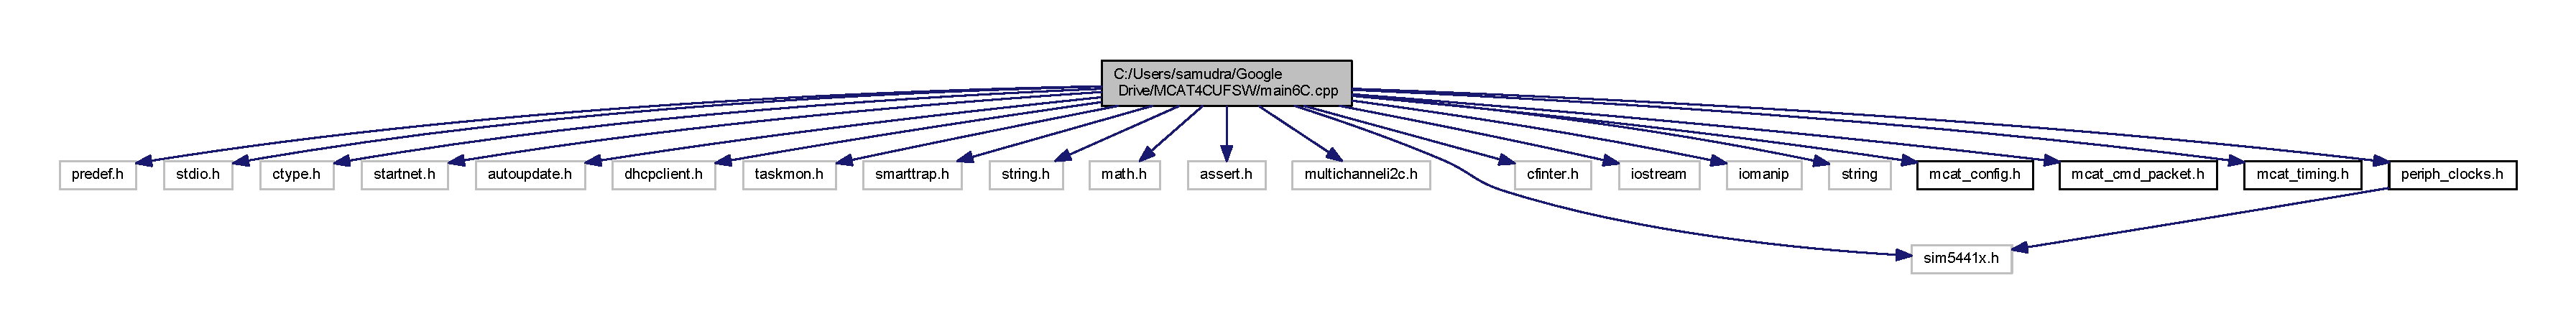
\includegraphics[width=350pt]{main6_c_8cpp__incl}
\end{center}
\end{figure}
\subsection*{Functions}
\begin{DoxyCompactItemize}
\item 
void \hyperlink{main6_c_8cpp_af3350bd69feae78ebcd4f766916eeb67}{parse\+C\+M\+D\+Packet} (char C\+M\+D\+Packet\mbox{[}I2\+C\+\_\+\+M\+A\+X\+\_\+\+B\+U\+F\+\_\+\+S\+I\+Z\+E\mbox{]})
\item 
void \hyperlink{main6_c_8cpp_aa3032893ba2f121a12d4cecf88277580}{parse\+Block\+G} (string Block\+G)
\item 
void \hyperlink{main6_c_8cpp_ab8ff54f4b027d2dfb6d3b63194fc15a4}{parse\+Block\+C\+U} (string Block\+C\+U)
\item 
void \hyperlink{main6_c_8cpp_a72e39dd7a2538b8b278f927ffd051bde}{parse\+Block\+I\+P\+D} (string Block\+I\+P\+D)
\item 
void \hyperlink{main6_c_8cpp_a8109658a433363943c469e7743c238ab}{parse\+Block\+P\+P\+U} (string Block\+P\+P\+U)
\item 
B\+Y\+T\+E \hyperlink{main6_c_8cpp_a22bb15ed96d4891d904b55838e451124}{Ascii2\+Byte} (char $\ast$buf)
\item 
void \hyperlink{main6_c_8cpp_ad16e5e62f3579a7048e6b981b172885e}{menu} (void)
\item 
void \hyperlink{main6_c_8cpp_ace7b2f4c33cbf41f3a43c7be01ff7aec}{User\+Main} (void $\ast$pd)
\item 
void \hyperlink{main6_c_8cpp_a486c7b37eb37847afaeeb6c73de398b9}{display\+Config} ()
\item 
void \hyperlink{main6_c_8cpp_a11ee600b69b27b0bb2d1b5b6e8ece140}{stop\+Pulses} (void $\ast$pdata)
\item 
void \hyperlink{main6_c_8cpp_a10570e6420ce0f0a076e1e9d3518d305}{init\+D\+M\+A\+T\+I\+M\+E\+R1} ()
\item 
void \hyperlink{main6_c_8cpp_a7c3f73193878c079945a21075f128059}{Set\+Intc} (long func, int vector, int level, int prio)
\item 
void \hyperlink{main6_c_8cpp_a8a64466bfb43094b3aec845670b959b4}{set\+Defaults} ()
\item 
void \hyperlink{main6_c_8cpp_a238885c747f586049b766fa4fcd5ec12}{disable\+All} ()
\item 
void \hyperlink{main6_c_8cpp_af2e78c1a970cd9490fcc3a5ac8015e6b}{debug\+Print} (string debug\+Msg)
\item 
\hyperlink{main6_c_8cpp_a89200d64c07024287b4ef31901f44e15}{I\+N\+T\+E\+R\+R\+U\+P\+T} (func\+\_\+isr, 0x2600)
\item 
void \hyperlink{main6_c_8cpp_acbfa28dfc2a41cc9cea58425f9b75178}{control\+P\+M\+A} (B\+O\+O\+L P\+M\+Flag)
\item 
void \hyperlink{main6_c_8cpp_ae4e046c7843050c83a5f70092acdbe1d}{control18\+L} (int requested\+Channel, int L\+Flag)
\item 
void \hyperlink{main6_c_8cpp_a2f5a551d47d5257bf34046aede82024e}{control18\+Hmanual} (int requested\+Channel, int H\+Flag)
\item 
void \hyperlink{main6_c_8cpp_a92a0eb6ae19d1612e39cbf1fd318d406}{set\+T\+P1} (long Frequency)
\item 
void \hyperlink{main6_c_8cpp_a8f5495a6630209795a3fbd7fa61a18e8}{control\+T\+P1} (B\+O\+O\+L T\+P1\+Flag)
\item 
void \hyperlink{main6_c_8cpp_a0ecec396fb6600a2f4897e7f30318159}{go\+F\+I\+R} ()
\item 
void \hyperlink{main6_c_8cpp_a2d0df7e0313c78e94bb4fafbc5752d67}{go\+F\+I\+Rfrom\+R\+U\+N} ()
\item 
void \hyperlink{main6_c_8cpp_ae0014243028b5cd808de963c18d01b11}{go\+F\+I\+Rfrom\+S\+B\+Y} ()
\item 
void \hyperlink{main6_c_8cpp_affc7dbdeb188c8169ccc6478143538d6}{go\+F\+I\+Rfrom\+I\+D\+L} ()
\item 
void \hyperlink{main6_c_8cpp_af57dea23daabb0f6e6d27f2ef21c9a54}{go\+R\+U\+N} ()
\item 
void \hyperlink{main6_c_8cpp_a6d712eb455e679cbf844c6742e7be6a0}{go\+R\+U\+Nfrom\+F\+I\+R} ()
\item 
void \hyperlink{main6_c_8cpp_a4770c1a01b1be1b23772d600b787d411}{go\+R\+U\+Nfrom\+S\+B\+Y} ()
\item 
void \hyperlink{main6_c_8cpp_a300391508ed006e4cd4ee0f9f316f3b4}{go\+R\+U\+Nfrom\+I\+D\+L} ()
\item 
void \hyperlink{main6_c_8cpp_a646dbe8155e1ee44efac5d50a7de878e}{go\+S\+B\+Y} ()
\item 
void \hyperlink{main6_c_8cpp_ae0ed43b60101aed3be6bea960293275d}{go\+S\+B\+Yfrom\+F\+I\+R} ()
\item 
void \hyperlink{main6_c_8cpp_a2d0b911e7b667c6a18000005acb28777}{go\+S\+B\+Yfrom\+R\+U\+N} ()
\item 
void \hyperlink{main6_c_8cpp_a37a57a2b0feb89b22b270931ae440c35}{go\+S\+B\+Yfrom\+I\+D\+L} ()
\item 
void \hyperlink{main6_c_8cpp_aa8d8f1cf694be5de1ac89b91627c0f51}{go\+I\+D\+L} ()
\item 
void \hyperlink{main6_c_8cpp_a3e3cc85ab7a91d6808984a0f78a5f9f8}{go\+I\+D\+Lfrom\+S\+B\+Y} ()
\item 
void \hyperlink{main6_c_8cpp_a690d16feac877ce7000b00e151dffd82}{go\+I\+D\+Lfrom\+R\+U\+N} ()
\item 
void \hyperlink{main6_c_8cpp_ae5438692f2a6c279129ecc19a91568f2}{go\+I\+D\+Lfrom\+F\+I\+R} ()
\item 
void \hyperlink{main6_c_8cpp_a9b07c4b395adfe387d12241e7ebaaae6}{set\+New\+Mode} (string cmd\+Mode\+Request, string \hyperlink{main6_c_8cpp_ab996ab5995af95792f5af3586d943d58}{cmd\+Mode\+Current})
\item 
void \hyperlink{main6_c_8cpp_ab482d6ef2e62e38354a2ab1d1e9827d3}{do\+Setup} ()
\item 
void \hyperlink{main6_c_8cpp_ae545852079ad06cd4f5cd017dd5c8249}{set\+New\+Pulse\+Count} ()
\item 
void \hyperlink{main6_c_8cpp_a8cbbd11ea6ebd5f8ad4a432646a65267}{disable\+Peripherals} ()
\end{DoxyCompactItemize}
\subsection*{Variables}
\begin{DoxyCompactItemize}
\item 
D\+W\+O\+R\+D \hyperlink{main6_c_8cpp_a1a81dd9879f21195e8d3b4d471524ccb}{start\+Pulse\+Count}
\item 
D\+W\+O\+R\+D \hyperlink{main6_c_8cpp_a694b66dde3c298b6b234344941a64bb9}{end\+Pulse\+Count}
\item 
B\+O\+O\+L \hyperlink{main6_c_8cpp_a5cbcba8bebc277fc9c0be941fdb92e82}{toggle\+H\+Flag}
\item 
char \hyperlink{main6_c_8cpp_a67cb76a345ef77fbb558f70971b6dc92}{id\+Q} \mbox{[}80\mbox{]}
\item 
char \hyperlink{main6_c_8cpp_a2dfc1feb8ca92d02b052fcb15b378560}{id\+C\+U} \mbox{[}160\mbox{]}
\item 
char \hyperlink{main6_c_8cpp_a9fbcbc3382bca9c438e08a693bc0369e}{ver\+C\+U} \mbox{[}2\mbox{]}
\item 
string \hyperlink{main6_c_8cpp_a405cdd34a0ec61abf8c5205c7a8c3182}{cmd\+Version} =\char`\"{}\char`\"{}
\item 
string \hyperlink{main6_c_8cpp_a8a9767341d04352fccd7068bc1d7c370}{cmd\+Mode} =\char`\"{}\char`\"{}
\item 
string \hyperlink{main6_c_8cpp_ab996ab5995af95792f5af3586d943d58}{cmd\+Mode\+Current} =\char`\"{}\char`\"{}
\item 
string \hyperlink{main6_c_8cpp_ad9049cc701250fb177b8e99713039762}{s\+\_\+freq\+T\+P1} =\char`\"{}\char`\"{}
\item 
string \hyperlink{main6_c_8cpp_a396dd1e7a6a9a4dc8b908980e2e1ded4}{s\+\_\+freq\+T\+P2} =\char`\"{}\char`\"{}
\item 
string \hyperlink{main6_c_8cpp_a62d24bc7666ac0bb0d8728dba649a256}{s\+\_\+freq\+T\+P3} =\char`\"{}\char`\"{}
\item 
string \hyperlink{main6_c_8cpp_a6a2b49919f4f32a4af53700ed1cde8ed}{s\+\_\+freq\+T\+P4} =\char`\"{}\char`\"{}
\item 
string \hyperlink{main6_c_8cpp_a4ba85625fa845776a2d64a3f58f36c42}{s\+\_\+count\+Ch1} =\char`\"{}\char`\"{}
\item 
string \hyperlink{main6_c_8cpp_a88730d26d9b63cdf8e4ca277a76b638d}{s\+\_\+count\+Ch2} =\char`\"{}\char`\"{}
\item 
string \hyperlink{main6_c_8cpp_a09052171565a4f15cbfdbc2ebcdd3fff}{s\+\_\+count\+Ch3} =\char`\"{}\char`\"{}
\item 
string \hyperlink{main6_c_8cpp_a32bb7a1f63c92a94ec3d098853bd883b}{s\+\_\+count\+Ch4} =\char`\"{}\char`\"{}
\item 
long \hyperlink{main6_c_8cpp_a7d2353ca53d5b5b259a823a92b7b519e}{freq\+T\+P1} = 10
\item 
long \hyperlink{main6_c_8cpp_a511164d7a4515d9a1f07ccfbda7ea294}{freq\+T\+P2} = 10
\item 
long \hyperlink{main6_c_8cpp_afae1443270cbb13745f612d5425f94a7}{freq\+T\+P3} = 10
\item 
long \hyperlink{main6_c_8cpp_a7cc56f796c77e7b30948d992bacc0429}{freq\+T\+P4} = 10
\item 
long \hyperlink{main6_c_8cpp_a9a1f402dd7e47f25ca3aa9ae7a8d0dc6}{count\+Ch1} = 0
\item 
long \hyperlink{main6_c_8cpp_a49801da896cbdab7c4b39b8e012c1a18}{count\+Ch2} = 0
\item 
long \hyperlink{main6_c_8cpp_a0582794ca95bdcf8787638b7def0177c}{count\+Ch3} = 0
\item 
long \hyperlink{main6_c_8cpp_a1de46864f078711d257187f01dfff541}{count\+Ch4} = 0
\item 
string \hyperlink{main6_c_8cpp_a37ec136ae86c4b7dc81f393bb1a01af7}{s\+\_\+cmd\+P18\+H1} =\char`\"{}\char`\"{}
\item 
string \hyperlink{main6_c_8cpp_a46ce373f60085f5900464cd0731fa20e}{s\+\_\+cmd\+P18\+H2} =\char`\"{}\char`\"{}
\item 
string \hyperlink{main6_c_8cpp_a909acdc96889fb5885793e8bc70b083e}{s\+\_\+cmd\+P18\+H3} =\char`\"{}\char`\"{}
\item 
string \hyperlink{main6_c_8cpp_a607e82175ad61b864bfa84e686437947}{s\+\_\+cmd\+P18\+H4} =\char`\"{}\char`\"{}
\item 
bool \hyperlink{main6_c_8cpp_a1a10d6a42e7c3ba1ad7f396b687a7eb7}{cmd\+P18\+H1}
\item 
bool \hyperlink{main6_c_8cpp_a03df8cc8ee6b4d7ba8a3d2ad50914508}{cmd\+P18\+H2}
\item 
bool \hyperlink{main6_c_8cpp_aba803fecbea259c5af71f0b9f2e9fa5a}{cmd\+P18\+H3}
\item 
bool \hyperlink{main6_c_8cpp_a74d16dd0ede9be1a1645027bd2e6fb21}{cmd\+P18\+H4}
\item 
B\+Y\+T\+E \hyperlink{main6_c_8cpp_a750abfb0120c1735c922980bd47640a5}{buffer} \mbox{[}I2\+C\+\_\+\+M\+A\+X\+\_\+\+B\+U\+F\+\_\+\+S\+I\+Z\+E\mbox{]}
\item 
char \hyperlink{main6_c_8cpp_af54d77a991da4ba360d594c2589140df}{I2\+C\+Input\+Buffer} \mbox{[}I2\+C\+\_\+\+M\+A\+X\+\_\+\+B\+U\+F\+\_\+\+S\+I\+Z\+E\mbox{]}
\item 
char $\ast$ \hyperlink{main6_c_8cpp_abed0c40696905e144ed4118061acf700}{inbuf} = \hyperlink{_v2_01main_8cpp_af54d77a991da4ba360d594c2589140df}{I2\+C\+Input\+Buffer}
\item 
B\+Y\+T\+E \hyperlink{main6_c_8cpp_a92fb5ea5b6a7d108dea33dd07809152d}{address} = \hyperlink{mcatsubsystemconfig_8h_a8fe248bd745b90e2bfe94d8c5fce0a53}{C\+U\+\_\+\+I2\+C\+\_\+\+S\+L\+A\+V\+E\+\_\+\+A\+D\+D\+R}
\item 
B\+Y\+T\+E \hyperlink{main6_c_8cpp_a6c3dedd37414833dd07e72ee4a642d13}{I2\+C\+Stat}
\item 
string \hyperlink{main6_c_8cpp_a7bd808a410bfdf94391ce02a61b3c1a7}{menu\+Version}
\end{DoxyCompactItemize}


\subsection{Function Documentation}
\hypertarget{main6_c_8cpp_a22bb15ed96d4891d904b55838e451124}{}\index{main6\+C.\+cpp@{main6\+C.\+cpp}!Ascii2\+Byte@{Ascii2\+Byte}}
\index{Ascii2\+Byte@{Ascii2\+Byte}!main6\+C.\+cpp@{main6\+C.\+cpp}}
\subsubsection[{Ascii2\+Byte}]{\setlength{\rightskip}{0pt plus 5cm}B\+Y\+T\+E Ascii2\+Byte (
\begin{DoxyParamCaption}
\item[{char $\ast$}]{buf}
\end{DoxyParamCaption}
)}\label{main6_c_8cpp_a22bb15ed96d4891d904b55838e451124}


Definition at line 1215 of file main6\+C.\+cpp.

\hypertarget{main6_c_8cpp_a2f5a551d47d5257bf34046aede82024e}{}\index{main6\+C.\+cpp@{main6\+C.\+cpp}!control18\+Hmanual@{control18\+Hmanual}}
\index{control18\+Hmanual@{control18\+Hmanual}!main6\+C.\+cpp@{main6\+C.\+cpp}}
\subsubsection[{control18\+Hmanual}]{\setlength{\rightskip}{0pt plus 5cm}void control18\+Hmanual (
\begin{DoxyParamCaption}
\item[{int}]{requested\+Channel, }
\item[{int}]{H\+Flag}
\end{DoxyParamCaption}
)}\label{main6_c_8cpp_a2f5a551d47d5257bf34046aede82024e}


Definition at line 376 of file main6\+C.\+cpp.

\hypertarget{main6_c_8cpp_ae4e046c7843050c83a5f70092acdbe1d}{}\index{main6\+C.\+cpp@{main6\+C.\+cpp}!control18\+L@{control18\+L}}
\index{control18\+L@{control18\+L}!main6\+C.\+cpp@{main6\+C.\+cpp}}
\subsubsection[{control18\+L}]{\setlength{\rightskip}{0pt plus 5cm}void control18\+L (
\begin{DoxyParamCaption}
\item[{int}]{requested\+Channel, }
\item[{int}]{L\+Flag}
\end{DoxyParamCaption}
)}\label{main6_c_8cpp_ae4e046c7843050c83a5f70092acdbe1d}


Definition at line 254 of file main6\+C.\+cpp.

\hypertarget{main6_c_8cpp_acbfa28dfc2a41cc9cea58425f9b75178}{}\index{main6\+C.\+cpp@{main6\+C.\+cpp}!control\+P\+M\+A@{control\+P\+M\+A}}
\index{control\+P\+M\+A@{control\+P\+M\+A}!main6\+C.\+cpp@{main6\+C.\+cpp}}
\subsubsection[{control\+P\+M\+A}]{\setlength{\rightskip}{0pt plus 5cm}void control\+P\+M\+A (
\begin{DoxyParamCaption}
\item[{B\+O\+O\+L}]{P\+M\+Flag}
\end{DoxyParamCaption}
)}\label{main6_c_8cpp_acbfa28dfc2a41cc9cea58425f9b75178}


Definition at line 237 of file main6\+C.\+cpp.

\hypertarget{main6_c_8cpp_a8f5495a6630209795a3fbd7fa61a18e8}{}\index{main6\+C.\+cpp@{main6\+C.\+cpp}!control\+T\+P1@{control\+T\+P1}}
\index{control\+T\+P1@{control\+T\+P1}!main6\+C.\+cpp@{main6\+C.\+cpp}}
\subsubsection[{control\+T\+P1}]{\setlength{\rightskip}{0pt plus 5cm}void control\+T\+P1 (
\begin{DoxyParamCaption}
\item[{B\+O\+O\+L}]{T\+P1\+Flag}
\end{DoxyParamCaption}
)}\label{main6_c_8cpp_a8f5495a6630209795a3fbd7fa61a18e8}
from 5270 code set /// D\+O N\+O\+T U\+S\+E Set\+Intc((long) \&func\+\_\+isr, 19, 1, 1); 

Definition at line 568 of file main6\+C.\+cpp.

\hypertarget{main6_c_8cpp_af2e78c1a970cd9490fcc3a5ac8015e6b}{}\index{main6\+C.\+cpp@{main6\+C.\+cpp}!debug\+Print@{debug\+Print}}
\index{debug\+Print@{debug\+Print}!main6\+C.\+cpp@{main6\+C.\+cpp}}
\subsubsection[{debug\+Print}]{\setlength{\rightskip}{0pt plus 5cm}void debug\+Print (
\begin{DoxyParamCaption}
\item[{string}]{debug\+Msg}
\end{DoxyParamCaption}
)}\label{main6_c_8cpp_af2e78c1a970cd9490fcc3a5ac8015e6b}


Definition at line 162 of file main6\+C.\+cpp.

\hypertarget{main6_c_8cpp_a238885c747f586049b766fa4fcd5ec12}{}\index{main6\+C.\+cpp@{main6\+C.\+cpp}!disable\+All@{disable\+All}}
\index{disable\+All@{disable\+All}!main6\+C.\+cpp@{main6\+C.\+cpp}}
\subsubsection[{disable\+All}]{\setlength{\rightskip}{0pt plus 5cm}void disable\+All (
\begin{DoxyParamCaption}
{}
\end{DoxyParamCaption}
)}\label{main6_c_8cpp_a238885c747f586049b766fa4fcd5ec12}


Definition at line 780 of file main6\+C.\+cpp.

\hypertarget{main6_c_8cpp_a8cbbd11ea6ebd5f8ad4a432646a65267}{}\index{main6\+C.\+cpp@{main6\+C.\+cpp}!disable\+Peripherals@{disable\+Peripherals}}
\index{disable\+Peripherals@{disable\+Peripherals}!main6\+C.\+cpp@{main6\+C.\+cpp}}
\subsubsection[{disable\+Peripherals}]{\setlength{\rightskip}{0pt plus 5cm}void disable\+Peripherals (
\begin{DoxyParamCaption}
{}
\end{DoxyParamCaption}
)}\label{main6_c_8cpp_a8cbbd11ea6ebd5f8ad4a432646a65267}


Definition at line 1334 of file main6\+C.\+cpp.

\hypertarget{main6_c_8cpp_a486c7b37eb37847afaeeb6c73de398b9}{}\index{main6\+C.\+cpp@{main6\+C.\+cpp}!display\+Config@{display\+Config}}
\index{display\+Config@{display\+Config}!main6\+C.\+cpp@{main6\+C.\+cpp}}
\subsubsection[{display\+Config}]{\setlength{\rightskip}{0pt plus 5cm}void display\+Config (
\begin{DoxyParamCaption}
{}
\end{DoxyParamCaption}
)}\label{main6_c_8cpp_a486c7b37eb37847afaeeb6c73de398b9}
\hypertarget{main6_c_8cpp_ab482d6ef2e62e38354a2ab1d1e9827d3}{}\index{main6\+C.\+cpp@{main6\+C.\+cpp}!do\+Setup@{do\+Setup}}
\index{do\+Setup@{do\+Setup}!main6\+C.\+cpp@{main6\+C.\+cpp}}
\subsubsection[{do\+Setup}]{\setlength{\rightskip}{0pt plus 5cm}void do\+Setup (
\begin{DoxyParamCaption}
{}
\end{DoxyParamCaption}
)}\label{main6_c_8cpp_ab482d6ef2e62e38354a2ab1d1e9827d3}


Definition at line 841 of file main6\+C.\+cpp.

\hypertarget{main6_c_8cpp_a0ecec396fb6600a2f4897e7f30318159}{}\index{main6\+C.\+cpp@{main6\+C.\+cpp}!go\+F\+I\+R@{go\+F\+I\+R}}
\index{go\+F\+I\+R@{go\+F\+I\+R}!main6\+C.\+cpp@{main6\+C.\+cpp}}
\subsubsection[{go\+F\+I\+R}]{\setlength{\rightskip}{0pt plus 5cm}void go\+F\+I\+R (
\begin{DoxyParamCaption}
{}
\end{DoxyParamCaption}
)}\label{main6_c_8cpp_a0ecec396fb6600a2f4897e7f30318159}


Definition at line 602 of file main6\+C.\+cpp.

\hypertarget{main6_c_8cpp_affc7dbdeb188c8169ccc6478143538d6}{}\index{main6\+C.\+cpp@{main6\+C.\+cpp}!go\+F\+I\+Rfrom\+I\+D\+L@{go\+F\+I\+Rfrom\+I\+D\+L}}
\index{go\+F\+I\+Rfrom\+I\+D\+L@{go\+F\+I\+Rfrom\+I\+D\+L}!main6\+C.\+cpp@{main6\+C.\+cpp}}
\subsubsection[{go\+F\+I\+Rfrom\+I\+D\+L}]{\setlength{\rightskip}{0pt plus 5cm}void go\+F\+I\+Rfrom\+I\+D\+L (
\begin{DoxyParamCaption}
{}
\end{DoxyParamCaption}
)}\label{main6_c_8cpp_affc7dbdeb188c8169ccc6478143538d6}


Definition at line 636 of file main6\+C.\+cpp.

\hypertarget{main6_c_8cpp_a2d0df7e0313c78e94bb4fafbc5752d67}{}\index{main6\+C.\+cpp@{main6\+C.\+cpp}!go\+F\+I\+Rfrom\+R\+U\+N@{go\+F\+I\+Rfrom\+R\+U\+N}}
\index{go\+F\+I\+Rfrom\+R\+U\+N@{go\+F\+I\+Rfrom\+R\+U\+N}!main6\+C.\+cpp@{main6\+C.\+cpp}}
\subsubsection[{go\+F\+I\+Rfrom\+R\+U\+N}]{\setlength{\rightskip}{0pt plus 5cm}void go\+F\+I\+Rfrom\+R\+U\+N (
\begin{DoxyParamCaption}
{}
\end{DoxyParamCaption}
)}\label{main6_c_8cpp_a2d0df7e0313c78e94bb4fafbc5752d67}


Definition at line 607 of file main6\+C.\+cpp.

\hypertarget{main6_c_8cpp_ae0014243028b5cd808de963c18d01b11}{}\index{main6\+C.\+cpp@{main6\+C.\+cpp}!go\+F\+I\+Rfrom\+S\+B\+Y@{go\+F\+I\+Rfrom\+S\+B\+Y}}
\index{go\+F\+I\+Rfrom\+S\+B\+Y@{go\+F\+I\+Rfrom\+S\+B\+Y}!main6\+C.\+cpp@{main6\+C.\+cpp}}
\subsubsection[{go\+F\+I\+Rfrom\+S\+B\+Y}]{\setlength{\rightskip}{0pt plus 5cm}void go\+F\+I\+Rfrom\+S\+B\+Y (
\begin{DoxyParamCaption}
{}
\end{DoxyParamCaption}
)}\label{main6_c_8cpp_ae0014243028b5cd808de963c18d01b11}


Definition at line 632 of file main6\+C.\+cpp.

\hypertarget{main6_c_8cpp_aa8d8f1cf694be5de1ac89b91627c0f51}{}\index{main6\+C.\+cpp@{main6\+C.\+cpp}!go\+I\+D\+L@{go\+I\+D\+L}}
\index{go\+I\+D\+L@{go\+I\+D\+L}!main6\+C.\+cpp@{main6\+C.\+cpp}}
\subsubsection[{go\+I\+D\+L}]{\setlength{\rightskip}{0pt plus 5cm}void go\+I\+D\+L (
\begin{DoxyParamCaption}
{}
\end{DoxyParamCaption}
)}\label{main6_c_8cpp_aa8d8f1cf694be5de1ac89b91627c0f51}


Definition at line 683 of file main6\+C.\+cpp.

\hypertarget{main6_c_8cpp_ae5438692f2a6c279129ecc19a91568f2}{}\index{main6\+C.\+cpp@{main6\+C.\+cpp}!go\+I\+D\+Lfrom\+F\+I\+R@{go\+I\+D\+Lfrom\+F\+I\+R}}
\index{go\+I\+D\+Lfrom\+F\+I\+R@{go\+I\+D\+Lfrom\+F\+I\+R}!main6\+C.\+cpp@{main6\+C.\+cpp}}
\subsubsection[{go\+I\+D\+Lfrom\+F\+I\+R}]{\setlength{\rightskip}{0pt plus 5cm}void go\+I\+D\+Lfrom\+F\+I\+R (
\begin{DoxyParamCaption}
{}
\end{DoxyParamCaption}
)}\label{main6_c_8cpp_ae5438692f2a6c279129ecc19a91568f2}


Definition at line 696 of file main6\+C.\+cpp.

\hypertarget{main6_c_8cpp_a690d16feac877ce7000b00e151dffd82}{}\index{main6\+C.\+cpp@{main6\+C.\+cpp}!go\+I\+D\+Lfrom\+R\+U\+N@{go\+I\+D\+Lfrom\+R\+U\+N}}
\index{go\+I\+D\+Lfrom\+R\+U\+N@{go\+I\+D\+Lfrom\+R\+U\+N}!main6\+C.\+cpp@{main6\+C.\+cpp}}
\subsubsection[{go\+I\+D\+Lfrom\+R\+U\+N}]{\setlength{\rightskip}{0pt plus 5cm}void go\+I\+D\+Lfrom\+R\+U\+N (
\begin{DoxyParamCaption}
{}
\end{DoxyParamCaption}
)}\label{main6_c_8cpp_a690d16feac877ce7000b00e151dffd82}


Definition at line 692 of file main6\+C.\+cpp.

\hypertarget{main6_c_8cpp_a3e3cc85ab7a91d6808984a0f78a5f9f8}{}\index{main6\+C.\+cpp@{main6\+C.\+cpp}!go\+I\+D\+Lfrom\+S\+B\+Y@{go\+I\+D\+Lfrom\+S\+B\+Y}}
\index{go\+I\+D\+Lfrom\+S\+B\+Y@{go\+I\+D\+Lfrom\+S\+B\+Y}!main6\+C.\+cpp@{main6\+C.\+cpp}}
\subsubsection[{go\+I\+D\+Lfrom\+S\+B\+Y}]{\setlength{\rightskip}{0pt plus 5cm}void go\+I\+D\+Lfrom\+S\+B\+Y (
\begin{DoxyParamCaption}
{}
\end{DoxyParamCaption}
)}\label{main6_c_8cpp_a3e3cc85ab7a91d6808984a0f78a5f9f8}


Definition at line 688 of file main6\+C.\+cpp.

\hypertarget{main6_c_8cpp_af57dea23daabb0f6e6d27f2ef21c9a54}{}\index{main6\+C.\+cpp@{main6\+C.\+cpp}!go\+R\+U\+N@{go\+R\+U\+N}}
\index{go\+R\+U\+N@{go\+R\+U\+N}!main6\+C.\+cpp@{main6\+C.\+cpp}}
\subsubsection[{go\+R\+U\+N}]{\setlength{\rightskip}{0pt plus 5cm}void go\+R\+U\+N (
\begin{DoxyParamCaption}
{}
\end{DoxyParamCaption}
)}\label{main6_c_8cpp_af57dea23daabb0f6e6d27f2ef21c9a54}


Definition at line 641 of file main6\+C.\+cpp.

\hypertarget{main6_c_8cpp_a6d712eb455e679cbf844c6742e7be6a0}{}\index{main6\+C.\+cpp@{main6\+C.\+cpp}!go\+R\+U\+Nfrom\+F\+I\+R@{go\+R\+U\+Nfrom\+F\+I\+R}}
\index{go\+R\+U\+Nfrom\+F\+I\+R@{go\+R\+U\+Nfrom\+F\+I\+R}!main6\+C.\+cpp@{main6\+C.\+cpp}}
\subsubsection[{go\+R\+U\+Nfrom\+F\+I\+R}]{\setlength{\rightskip}{0pt plus 5cm}void go\+R\+U\+Nfrom\+F\+I\+R (
\begin{DoxyParamCaption}
{}
\end{DoxyParamCaption}
)}\label{main6_c_8cpp_a6d712eb455e679cbf844c6742e7be6a0}


Definition at line 652 of file main6\+C.\+cpp.

\hypertarget{main6_c_8cpp_a300391508ed006e4cd4ee0f9f316f3b4}{}\index{main6\+C.\+cpp@{main6\+C.\+cpp}!go\+R\+U\+Nfrom\+I\+D\+L@{go\+R\+U\+Nfrom\+I\+D\+L}}
\index{go\+R\+U\+Nfrom\+I\+D\+L@{go\+R\+U\+Nfrom\+I\+D\+L}!main6\+C.\+cpp@{main6\+C.\+cpp}}
\subsubsection[{go\+R\+U\+Nfrom\+I\+D\+L}]{\setlength{\rightskip}{0pt plus 5cm}void go\+R\+U\+Nfrom\+I\+D\+L (
\begin{DoxyParamCaption}
{}
\end{DoxyParamCaption}
)}\label{main6_c_8cpp_a300391508ed006e4cd4ee0f9f316f3b4}


Definition at line 660 of file main6\+C.\+cpp.

\hypertarget{main6_c_8cpp_a4770c1a01b1be1b23772d600b787d411}{}\index{main6\+C.\+cpp@{main6\+C.\+cpp}!go\+R\+U\+Nfrom\+S\+B\+Y@{go\+R\+U\+Nfrom\+S\+B\+Y}}
\index{go\+R\+U\+Nfrom\+S\+B\+Y@{go\+R\+U\+Nfrom\+S\+B\+Y}!main6\+C.\+cpp@{main6\+C.\+cpp}}
\subsubsection[{go\+R\+U\+Nfrom\+S\+B\+Y}]{\setlength{\rightskip}{0pt plus 5cm}void go\+R\+U\+Nfrom\+S\+B\+Y (
\begin{DoxyParamCaption}
{}
\end{DoxyParamCaption}
)}\label{main6_c_8cpp_a4770c1a01b1be1b23772d600b787d411}


Definition at line 656 of file main6\+C.\+cpp.

\hypertarget{main6_c_8cpp_a646dbe8155e1ee44efac5d50a7de878e}{}\index{main6\+C.\+cpp@{main6\+C.\+cpp}!go\+S\+B\+Y@{go\+S\+B\+Y}}
\index{go\+S\+B\+Y@{go\+S\+B\+Y}!main6\+C.\+cpp@{main6\+C.\+cpp}}
\subsubsection[{go\+S\+B\+Y}]{\setlength{\rightskip}{0pt plus 5cm}void go\+S\+B\+Y (
\begin{DoxyParamCaption}
{}
\end{DoxyParamCaption}
)}\label{main6_c_8cpp_a646dbe8155e1ee44efac5d50a7de878e}


Definition at line 665 of file main6\+C.\+cpp.

\hypertarget{main6_c_8cpp_ae0ed43b60101aed3be6bea960293275d}{}\index{main6\+C.\+cpp@{main6\+C.\+cpp}!go\+S\+B\+Yfrom\+F\+I\+R@{go\+S\+B\+Yfrom\+F\+I\+R}}
\index{go\+S\+B\+Yfrom\+F\+I\+R@{go\+S\+B\+Yfrom\+F\+I\+R}!main6\+C.\+cpp@{main6\+C.\+cpp}}
\subsubsection[{go\+S\+B\+Yfrom\+F\+I\+R}]{\setlength{\rightskip}{0pt plus 5cm}void go\+S\+B\+Yfrom\+F\+I\+R (
\begin{DoxyParamCaption}
{}
\end{DoxyParamCaption}
)}\label{main6_c_8cpp_ae0ed43b60101aed3be6bea960293275d}


Definition at line 670 of file main6\+C.\+cpp.

\hypertarget{main6_c_8cpp_a37a57a2b0feb89b22b270931ae440c35}{}\index{main6\+C.\+cpp@{main6\+C.\+cpp}!go\+S\+B\+Yfrom\+I\+D\+L@{go\+S\+B\+Yfrom\+I\+D\+L}}
\index{go\+S\+B\+Yfrom\+I\+D\+L@{go\+S\+B\+Yfrom\+I\+D\+L}!main6\+C.\+cpp@{main6\+C.\+cpp}}
\subsubsection[{go\+S\+B\+Yfrom\+I\+D\+L}]{\setlength{\rightskip}{0pt plus 5cm}void go\+S\+B\+Yfrom\+I\+D\+L (
\begin{DoxyParamCaption}
{}
\end{DoxyParamCaption}
)}\label{main6_c_8cpp_a37a57a2b0feb89b22b270931ae440c35}


Definition at line 678 of file main6\+C.\+cpp.

\hypertarget{main6_c_8cpp_a2d0b911e7b667c6a18000005acb28777}{}\index{main6\+C.\+cpp@{main6\+C.\+cpp}!go\+S\+B\+Yfrom\+R\+U\+N@{go\+S\+B\+Yfrom\+R\+U\+N}}
\index{go\+S\+B\+Yfrom\+R\+U\+N@{go\+S\+B\+Yfrom\+R\+U\+N}!main6\+C.\+cpp@{main6\+C.\+cpp}}
\subsubsection[{go\+S\+B\+Yfrom\+R\+U\+N}]{\setlength{\rightskip}{0pt plus 5cm}void go\+S\+B\+Yfrom\+R\+U\+N (
\begin{DoxyParamCaption}
{}
\end{DoxyParamCaption}
)}\label{main6_c_8cpp_a2d0b911e7b667c6a18000005acb28777}


Definition at line 674 of file main6\+C.\+cpp.

\hypertarget{main6_c_8cpp_a10570e6420ce0f0a076e1e9d3518d305}{}\index{main6\+C.\+cpp@{main6\+C.\+cpp}!init\+D\+M\+A\+T\+I\+M\+E\+R1@{init\+D\+M\+A\+T\+I\+M\+E\+R1}}
\index{init\+D\+M\+A\+T\+I\+M\+E\+R1@{init\+D\+M\+A\+T\+I\+M\+E\+R1}!main6\+C.\+cpp@{main6\+C.\+cpp}}
\subsubsection[{init\+D\+M\+A\+T\+I\+M\+E\+R1}]{\setlength{\rightskip}{0pt plus 5cm}void init\+D\+M\+A\+T\+I\+M\+E\+R1 (
\begin{DoxyParamCaption}
{}
\end{DoxyParamCaption}
)}\label{main6_c_8cpp_a10570e6420ce0f0a076e1e9d3518d305}
from 5270 code set /// D\+O N\+O\+T U\+S\+E Set\+Intc((long) \&func\+\_\+isr, 19, 1, 1); 

Definition at line 826 of file main6\+C.\+cpp.

\hypertarget{main6_c_8cpp_a89200d64c07024287b4ef31901f44e15}{}\index{main6\+C.\+cpp@{main6\+C.\+cpp}!I\+N\+T\+E\+R\+R\+U\+P\+T@{I\+N\+T\+E\+R\+R\+U\+P\+T}}
\index{I\+N\+T\+E\+R\+R\+U\+P\+T@{I\+N\+T\+E\+R\+R\+U\+P\+T}!main6\+C.\+cpp@{main6\+C.\+cpp}}
\subsubsection[{I\+N\+T\+E\+R\+R\+U\+P\+T}]{\setlength{\rightskip}{0pt plus 5cm}I\+N\+T\+E\+R\+R\+U\+P\+T (
\begin{DoxyParamCaption}
\item[{func\+\_\+isr}]{, }
\item[{0x2600}]{}
\end{DoxyParamCaption}
)}\label{main6_c_8cpp_a89200d64c07024287b4ef31901f44e15}


Definition at line 170 of file main6\+C.\+cpp.

\hypertarget{main6_c_8cpp_ad16e5e62f3579a7048e6b981b172885e}{}\index{main6\+C.\+cpp@{main6\+C.\+cpp}!menu@{menu}}
\index{menu@{menu}!main6\+C.\+cpp@{main6\+C.\+cpp}}
\subsubsection[{menu}]{\setlength{\rightskip}{0pt plus 5cm}void menu (
\begin{DoxyParamCaption}
\item[{void}]{}
\end{DoxyParamCaption}
)}\label{main6_c_8cpp_ad16e5e62f3579a7048e6b981b172885e}


Definition at line 1233 of file main6\+C.\+cpp.

\hypertarget{main6_c_8cpp_ab8ff54f4b027d2dfb6d3b63194fc15a4}{}\index{main6\+C.\+cpp@{main6\+C.\+cpp}!parse\+Block\+C\+U@{parse\+Block\+C\+U}}
\index{parse\+Block\+C\+U@{parse\+Block\+C\+U}!main6\+C.\+cpp@{main6\+C.\+cpp}}
\subsubsection[{parse\+Block\+C\+U}]{\setlength{\rightskip}{0pt plus 5cm}void parse\+Block\+C\+U (
\begin{DoxyParamCaption}
\item[{string}]{Block\+C\+U}
\end{DoxyParamCaption}
)}\label{main6_c_8cpp_ab8ff54f4b027d2dfb6d3b63194fc15a4}


Definition at line 1089 of file main6\+C.\+cpp.

\hypertarget{main6_c_8cpp_aa3032893ba2f121a12d4cecf88277580}{}\index{main6\+C.\+cpp@{main6\+C.\+cpp}!parse\+Block\+G@{parse\+Block\+G}}
\index{parse\+Block\+G@{parse\+Block\+G}!main6\+C.\+cpp@{main6\+C.\+cpp}}
\subsubsection[{parse\+Block\+G}]{\setlength{\rightskip}{0pt plus 5cm}void parse\+Block\+G (
\begin{DoxyParamCaption}
\item[{string}]{Block\+G}
\end{DoxyParamCaption}
)}\label{main6_c_8cpp_aa3032893ba2f121a12d4cecf88277580}


Definition at line 1079 of file main6\+C.\+cpp.

\hypertarget{main6_c_8cpp_a72e39dd7a2538b8b278f927ffd051bde}{}\index{main6\+C.\+cpp@{main6\+C.\+cpp}!parse\+Block\+I\+P\+D@{parse\+Block\+I\+P\+D}}
\index{parse\+Block\+I\+P\+D@{parse\+Block\+I\+P\+D}!main6\+C.\+cpp@{main6\+C.\+cpp}}
\subsubsection[{parse\+Block\+I\+P\+D}]{\setlength{\rightskip}{0pt plus 5cm}void parse\+Block\+I\+P\+D (
\begin{DoxyParamCaption}
\item[{string}]{Block\+I\+P\+D}
\end{DoxyParamCaption}
)}\label{main6_c_8cpp_a72e39dd7a2538b8b278f927ffd051bde}


Definition at line 1100 of file main6\+C.\+cpp.

\hypertarget{main6_c_8cpp_a8109658a433363943c469e7743c238ab}{}\index{main6\+C.\+cpp@{main6\+C.\+cpp}!parse\+Block\+P\+P\+U@{parse\+Block\+P\+P\+U}}
\index{parse\+Block\+P\+P\+U@{parse\+Block\+P\+P\+U}!main6\+C.\+cpp@{main6\+C.\+cpp}}
\subsubsection[{parse\+Block\+P\+P\+U}]{\setlength{\rightskip}{0pt plus 5cm}void parse\+Block\+P\+P\+U (
\begin{DoxyParamCaption}
\item[{string}]{Block\+P\+P\+U}
\end{DoxyParamCaption}
)}\label{main6_c_8cpp_a8109658a433363943c469e7743c238ab}


Definition at line 1155 of file main6\+C.\+cpp.

\hypertarget{main6_c_8cpp_af3350bd69feae78ebcd4f766916eeb67}{}\index{main6\+C.\+cpp@{main6\+C.\+cpp}!parse\+C\+M\+D\+Packet@{parse\+C\+M\+D\+Packet}}
\index{parse\+C\+M\+D\+Packet@{parse\+C\+M\+D\+Packet}!main6\+C.\+cpp@{main6\+C.\+cpp}}
\subsubsection[{parse\+C\+M\+D\+Packet}]{\setlength{\rightskip}{0pt plus 5cm}void parse\+C\+M\+D\+Packet (
\begin{DoxyParamCaption}
\item[{char}]{C\+M\+D\+Packet\mbox{[}\+I2\+C\+\_\+\+M\+A\+X\+\_\+\+B\+U\+F\+\_\+\+S\+I\+Z\+E\mbox{]}}
\end{DoxyParamCaption}
)}\label{main6_c_8cpp_af3350bd69feae78ebcd4f766916eeb67}


Definition at line 934 of file main6\+C.\+cpp.

\hypertarget{main6_c_8cpp_a8a64466bfb43094b3aec845670b959b4}{}\index{main6\+C.\+cpp@{main6\+C.\+cpp}!set\+Defaults@{set\+Defaults}}
\index{set\+Defaults@{set\+Defaults}!main6\+C.\+cpp@{main6\+C.\+cpp}}
\subsubsection[{set\+Defaults}]{\setlength{\rightskip}{0pt plus 5cm}void set\+Defaults (
\begin{DoxyParamCaption}
{}
\end{DoxyParamCaption}
)}\label{main6_c_8cpp_a8a64466bfb43094b3aec845670b959b4}


Definition at line 787 of file main6\+C.\+cpp.

\hypertarget{main6_c_8cpp_a7c3f73193878c079945a21075f128059}{}\index{main6\+C.\+cpp@{main6\+C.\+cpp}!Set\+Intc@{Set\+Intc}}
\index{Set\+Intc@{Set\+Intc}!main6\+C.\+cpp@{main6\+C.\+cpp}}
\subsubsection[{Set\+Intc}]{\setlength{\rightskip}{0pt plus 5cm}void Set\+Intc (
\begin{DoxyParamCaption}
\item[{long}]{func, }
\item[{int}]{vector, }
\item[{int}]{level, }
\item[{int}]{prio}
\end{DoxyParamCaption}
)}\label{main6_c_8cpp_a7c3f73193878c079945a21075f128059}
\hypertarget{main6_c_8cpp_a9b07c4b395adfe387d12241e7ebaaae6}{}\index{main6\+C.\+cpp@{main6\+C.\+cpp}!set\+New\+Mode@{set\+New\+Mode}}
\index{set\+New\+Mode@{set\+New\+Mode}!main6\+C.\+cpp@{main6\+C.\+cpp}}
\subsubsection[{set\+New\+Mode}]{\setlength{\rightskip}{0pt plus 5cm}void set\+New\+Mode (
\begin{DoxyParamCaption}
\item[{string}]{cmd\+Mode\+Request, }
\item[{string}]{cmd\+Mode\+Current}
\end{DoxyParamCaption}
)}\label{main6_c_8cpp_a9b07c4b395adfe387d12241e7ebaaae6}


Definition at line 703 of file main6\+C.\+cpp.

\hypertarget{main6_c_8cpp_ae545852079ad06cd4f5cd017dd5c8249}{}\index{main6\+C.\+cpp@{main6\+C.\+cpp}!set\+New\+Pulse\+Count@{set\+New\+Pulse\+Count}}
\index{set\+New\+Pulse\+Count@{set\+New\+Pulse\+Count}!main6\+C.\+cpp@{main6\+C.\+cpp}}
\subsubsection[{set\+New\+Pulse\+Count}]{\setlength{\rightskip}{0pt plus 5cm}void set\+New\+Pulse\+Count (
\begin{DoxyParamCaption}
{}
\end{DoxyParamCaption}
)}\label{main6_c_8cpp_ae545852079ad06cd4f5cd017dd5c8249}


Definition at line 1323 of file main6\+C.\+cpp.

\hypertarget{main6_c_8cpp_a92a0eb6ae19d1612e39cbf1fd318d406}{}\index{main6\+C.\+cpp@{main6\+C.\+cpp}!set\+T\+P1@{set\+T\+P1}}
\index{set\+T\+P1@{set\+T\+P1}!main6\+C.\+cpp@{main6\+C.\+cpp}}
\subsubsection[{set\+T\+P1}]{\setlength{\rightskip}{0pt plus 5cm}void set\+T\+P1 (
\begin{DoxyParamCaption}
\item[{long}]{Frequency}
\end{DoxyParamCaption}
)}\label{main6_c_8cpp_a92a0eb6ae19d1612e39cbf1fd318d406}


Definition at line 547 of file main6\+C.\+cpp.

\hypertarget{main6_c_8cpp_a11ee600b69b27b0bb2d1b5b6e8ece140}{}\index{main6\+C.\+cpp@{main6\+C.\+cpp}!stop\+Pulses@{stop\+Pulses}}
\index{stop\+Pulses@{stop\+Pulses}!main6\+C.\+cpp@{main6\+C.\+cpp}}
\subsubsection[{stop\+Pulses}]{\setlength{\rightskip}{0pt plus 5cm}void stop\+Pulses (
\begin{DoxyParamCaption}
\item[{void $\ast$}]{pdata}
\end{DoxyParamCaption}
)}\label{main6_c_8cpp_a11ee600b69b27b0bb2d1b5b6e8ece140}
\hypertarget{main6_c_8cpp_ace7b2f4c33cbf41f3a43c7be01ff7aec}{}\index{main6\+C.\+cpp@{main6\+C.\+cpp}!User\+Main@{User\+Main}}
\index{User\+Main@{User\+Main}!main6\+C.\+cpp@{main6\+C.\+cpp}}
\subsubsection[{User\+Main}]{\setlength{\rightskip}{0pt plus 5cm}void User\+Main (
\begin{DoxyParamCaption}
\item[{void $\ast$}]{pd}
\end{DoxyParamCaption}
)}\label{main6_c_8cpp_ace7b2f4c33cbf41f3a43c7be01ff7aec}
Thruster Channel P18 activation section

C\+H1-\/4

End Thruster Channel P18 activation section 

Definition at line 1380 of file main6\+C.\+cpp.



\subsection{Variable Documentation}
\hypertarget{main6_c_8cpp_a92fb5ea5b6a7d108dea33dd07809152d}{}\index{main6\+C.\+cpp@{main6\+C.\+cpp}!address@{address}}
\index{address@{address}!main6\+C.\+cpp@{main6\+C.\+cpp}}
\subsubsection[{address}]{\setlength{\rightskip}{0pt plus 5cm}B\+Y\+T\+E address = {\bf C\+U\+\_\+\+I2\+C\+\_\+\+S\+L\+A\+V\+E\+\_\+\+A\+D\+D\+R}}\label{main6_c_8cpp_a92fb5ea5b6a7d108dea33dd07809152d}


Definition at line 155 of file main6\+C.\+cpp.

\hypertarget{main6_c_8cpp_a750abfb0120c1735c922980bd47640a5}{}\index{main6\+C.\+cpp@{main6\+C.\+cpp}!buffer@{buffer}}
\index{buffer@{buffer}!main6\+C.\+cpp@{main6\+C.\+cpp}}
\subsubsection[{buffer}]{\setlength{\rightskip}{0pt plus 5cm}B\+Y\+T\+E buffer\mbox{[}I2\+C\+\_\+\+M\+A\+X\+\_\+\+B\+U\+F\+\_\+\+S\+I\+Z\+E\mbox{]}}\label{main6_c_8cpp_a750abfb0120c1735c922980bd47640a5}


Definition at line 152 of file main6\+C.\+cpp.

\hypertarget{main6_c_8cpp_a8a9767341d04352fccd7068bc1d7c370}{}\index{main6\+C.\+cpp@{main6\+C.\+cpp}!cmd\+Mode@{cmd\+Mode}}
\index{cmd\+Mode@{cmd\+Mode}!main6\+C.\+cpp@{main6\+C.\+cpp}}
\subsubsection[{cmd\+Mode}]{\setlength{\rightskip}{0pt plus 5cm}string cmd\+Mode =\char`\"{}\char`\"{}}\label{main6_c_8cpp_a8a9767341d04352fccd7068bc1d7c370}


Definition at line 74 of file main6\+C.\+cpp.

\hypertarget{main6_c_8cpp_ab996ab5995af95792f5af3586d943d58}{}\index{main6\+C.\+cpp@{main6\+C.\+cpp}!cmd\+Mode\+Current@{cmd\+Mode\+Current}}
\index{cmd\+Mode\+Current@{cmd\+Mode\+Current}!main6\+C.\+cpp@{main6\+C.\+cpp}}
\subsubsection[{cmd\+Mode\+Current}]{\setlength{\rightskip}{0pt plus 5cm}string cmd\+Mode\+Current =\char`\"{}\char`\"{}}\label{main6_c_8cpp_ab996ab5995af95792f5af3586d943d58}


Definition at line 75 of file main6\+C.\+cpp.

\hypertarget{main6_c_8cpp_a1a10d6a42e7c3ba1ad7f396b687a7eb7}{}\index{main6\+C.\+cpp@{main6\+C.\+cpp}!cmd\+P18\+H1@{cmd\+P18\+H1}}
\index{cmd\+P18\+H1@{cmd\+P18\+H1}!main6\+C.\+cpp@{main6\+C.\+cpp}}
\subsubsection[{cmd\+P18\+H1}]{\setlength{\rightskip}{0pt plus 5cm}bool cmd\+P18\+H1}\label{main6_c_8cpp_a1a10d6a42e7c3ba1ad7f396b687a7eb7}


Definition at line 97 of file main6\+C.\+cpp.

\hypertarget{main6_c_8cpp_a03df8cc8ee6b4d7ba8a3d2ad50914508}{}\index{main6\+C.\+cpp@{main6\+C.\+cpp}!cmd\+P18\+H2@{cmd\+P18\+H2}}
\index{cmd\+P18\+H2@{cmd\+P18\+H2}!main6\+C.\+cpp@{main6\+C.\+cpp}}
\subsubsection[{cmd\+P18\+H2}]{\setlength{\rightskip}{0pt plus 5cm}bool cmd\+P18\+H2}\label{main6_c_8cpp_a03df8cc8ee6b4d7ba8a3d2ad50914508}


Definition at line 97 of file main6\+C.\+cpp.

\hypertarget{main6_c_8cpp_aba803fecbea259c5af71f0b9f2e9fa5a}{}\index{main6\+C.\+cpp@{main6\+C.\+cpp}!cmd\+P18\+H3@{cmd\+P18\+H3}}
\index{cmd\+P18\+H3@{cmd\+P18\+H3}!main6\+C.\+cpp@{main6\+C.\+cpp}}
\subsubsection[{cmd\+P18\+H3}]{\setlength{\rightskip}{0pt plus 5cm}bool cmd\+P18\+H3}\label{main6_c_8cpp_aba803fecbea259c5af71f0b9f2e9fa5a}


Definition at line 97 of file main6\+C.\+cpp.

\hypertarget{main6_c_8cpp_a74d16dd0ede9be1a1645027bd2e6fb21}{}\index{main6\+C.\+cpp@{main6\+C.\+cpp}!cmd\+P18\+H4@{cmd\+P18\+H4}}
\index{cmd\+P18\+H4@{cmd\+P18\+H4}!main6\+C.\+cpp@{main6\+C.\+cpp}}
\subsubsection[{cmd\+P18\+H4}]{\setlength{\rightskip}{0pt plus 5cm}bool cmd\+P18\+H4}\label{main6_c_8cpp_a74d16dd0ede9be1a1645027bd2e6fb21}


Definition at line 97 of file main6\+C.\+cpp.

\hypertarget{main6_c_8cpp_a405cdd34a0ec61abf8c5205c7a8c3182}{}\index{main6\+C.\+cpp@{main6\+C.\+cpp}!cmd\+Version@{cmd\+Version}}
\index{cmd\+Version@{cmd\+Version}!main6\+C.\+cpp@{main6\+C.\+cpp}}
\subsubsection[{cmd\+Version}]{\setlength{\rightskip}{0pt plus 5cm}string cmd\+Version =\char`\"{}\char`\"{}}\label{main6_c_8cpp_a405cdd34a0ec61abf8c5205c7a8c3182}


Definition at line 73 of file main6\+C.\+cpp.

\hypertarget{main6_c_8cpp_a9a1f402dd7e47f25ca3aa9ae7a8d0dc6}{}\index{main6\+C.\+cpp@{main6\+C.\+cpp}!count\+Ch1@{count\+Ch1}}
\index{count\+Ch1@{count\+Ch1}!main6\+C.\+cpp@{main6\+C.\+cpp}}
\subsubsection[{count\+Ch1}]{\setlength{\rightskip}{0pt plus 5cm}long count\+Ch1 = 0}\label{main6_c_8cpp_a9a1f402dd7e47f25ca3aa9ae7a8d0dc6}


Definition at line 89 of file main6\+C.\+cpp.

\hypertarget{main6_c_8cpp_a49801da896cbdab7c4b39b8e012c1a18}{}\index{main6\+C.\+cpp@{main6\+C.\+cpp}!count\+Ch2@{count\+Ch2}}
\index{count\+Ch2@{count\+Ch2}!main6\+C.\+cpp@{main6\+C.\+cpp}}
\subsubsection[{count\+Ch2}]{\setlength{\rightskip}{0pt plus 5cm}long count\+Ch2 = 0}\label{main6_c_8cpp_a49801da896cbdab7c4b39b8e012c1a18}


Definition at line 90 of file main6\+C.\+cpp.

\hypertarget{main6_c_8cpp_a0582794ca95bdcf8787638b7def0177c}{}\index{main6\+C.\+cpp@{main6\+C.\+cpp}!count\+Ch3@{count\+Ch3}}
\index{count\+Ch3@{count\+Ch3}!main6\+C.\+cpp@{main6\+C.\+cpp}}
\subsubsection[{count\+Ch3}]{\setlength{\rightskip}{0pt plus 5cm}long count\+Ch3 = 0}\label{main6_c_8cpp_a0582794ca95bdcf8787638b7def0177c}


Definition at line 91 of file main6\+C.\+cpp.

\hypertarget{main6_c_8cpp_a1de46864f078711d257187f01dfff541}{}\index{main6\+C.\+cpp@{main6\+C.\+cpp}!count\+Ch4@{count\+Ch4}}
\index{count\+Ch4@{count\+Ch4}!main6\+C.\+cpp@{main6\+C.\+cpp}}
\subsubsection[{count\+Ch4}]{\setlength{\rightskip}{0pt plus 5cm}long count\+Ch4 = 0}\label{main6_c_8cpp_a1de46864f078711d257187f01dfff541}


Definition at line 92 of file main6\+C.\+cpp.

\hypertarget{main6_c_8cpp_a694b66dde3c298b6b234344941a64bb9}{}\index{main6\+C.\+cpp@{main6\+C.\+cpp}!end\+Pulse\+Count@{end\+Pulse\+Count}}
\index{end\+Pulse\+Count@{end\+Pulse\+Count}!main6\+C.\+cpp@{main6\+C.\+cpp}}
\subsubsection[{end\+Pulse\+Count}]{\setlength{\rightskip}{0pt plus 5cm}D\+W\+O\+R\+D end\+Pulse\+Count}\label{main6_c_8cpp_a694b66dde3c298b6b234344941a64bb9}


Definition at line 68 of file main6\+C.\+cpp.

\hypertarget{main6_c_8cpp_a7d2353ca53d5b5b259a823a92b7b519e}{}\index{main6\+C.\+cpp@{main6\+C.\+cpp}!freq\+T\+P1@{freq\+T\+P1}}
\index{freq\+T\+P1@{freq\+T\+P1}!main6\+C.\+cpp@{main6\+C.\+cpp}}
\subsubsection[{freq\+T\+P1}]{\setlength{\rightskip}{0pt plus 5cm}long freq\+T\+P1 = 10}\label{main6_c_8cpp_a7d2353ca53d5b5b259a823a92b7b519e}


Definition at line 85 of file main6\+C.\+cpp.

\hypertarget{main6_c_8cpp_a511164d7a4515d9a1f07ccfbda7ea294}{}\index{main6\+C.\+cpp@{main6\+C.\+cpp}!freq\+T\+P2@{freq\+T\+P2}}
\index{freq\+T\+P2@{freq\+T\+P2}!main6\+C.\+cpp@{main6\+C.\+cpp}}
\subsubsection[{freq\+T\+P2}]{\setlength{\rightskip}{0pt plus 5cm}long freq\+T\+P2 = 10}\label{main6_c_8cpp_a511164d7a4515d9a1f07ccfbda7ea294}


Definition at line 86 of file main6\+C.\+cpp.

\hypertarget{main6_c_8cpp_afae1443270cbb13745f612d5425f94a7}{}\index{main6\+C.\+cpp@{main6\+C.\+cpp}!freq\+T\+P3@{freq\+T\+P3}}
\index{freq\+T\+P3@{freq\+T\+P3}!main6\+C.\+cpp@{main6\+C.\+cpp}}
\subsubsection[{freq\+T\+P3}]{\setlength{\rightskip}{0pt plus 5cm}long freq\+T\+P3 = 10}\label{main6_c_8cpp_afae1443270cbb13745f612d5425f94a7}


Definition at line 87 of file main6\+C.\+cpp.

\hypertarget{main6_c_8cpp_a7cc56f796c77e7b30948d992bacc0429}{}\index{main6\+C.\+cpp@{main6\+C.\+cpp}!freq\+T\+P4@{freq\+T\+P4}}
\index{freq\+T\+P4@{freq\+T\+P4}!main6\+C.\+cpp@{main6\+C.\+cpp}}
\subsubsection[{freq\+T\+P4}]{\setlength{\rightskip}{0pt plus 5cm}long freq\+T\+P4 = 10}\label{main6_c_8cpp_a7cc56f796c77e7b30948d992bacc0429}


Definition at line 88 of file main6\+C.\+cpp.

\hypertarget{main6_c_8cpp_af54d77a991da4ba360d594c2589140df}{}\index{main6\+C.\+cpp@{main6\+C.\+cpp}!I2\+C\+Input\+Buffer@{I2\+C\+Input\+Buffer}}
\index{I2\+C\+Input\+Buffer@{I2\+C\+Input\+Buffer}!main6\+C.\+cpp@{main6\+C.\+cpp}}
\subsubsection[{I2\+C\+Input\+Buffer}]{\setlength{\rightskip}{0pt plus 5cm}char I2\+C\+Input\+Buffer\mbox{[}I2\+C\+\_\+\+M\+A\+X\+\_\+\+B\+U\+F\+\_\+\+S\+I\+Z\+E\mbox{]}}\label{main6_c_8cpp_af54d77a991da4ba360d594c2589140df}


Definition at line 153 of file main6\+C.\+cpp.

\hypertarget{main6_c_8cpp_a6c3dedd37414833dd07e72ee4a642d13}{}\index{main6\+C.\+cpp@{main6\+C.\+cpp}!I2\+C\+Stat@{I2\+C\+Stat}}
\index{I2\+C\+Stat@{I2\+C\+Stat}!main6\+C.\+cpp@{main6\+C.\+cpp}}
\subsubsection[{I2\+C\+Stat}]{\setlength{\rightskip}{0pt plus 5cm}B\+Y\+T\+E I2\+C\+Stat}\label{main6_c_8cpp_a6c3dedd37414833dd07e72ee4a642d13}


Definition at line 156 of file main6\+C.\+cpp.

\hypertarget{main6_c_8cpp_a2dfc1feb8ca92d02b052fcb15b378560}{}\index{main6\+C.\+cpp@{main6\+C.\+cpp}!id\+C\+U@{id\+C\+U}}
\index{id\+C\+U@{id\+C\+U}!main6\+C.\+cpp@{main6\+C.\+cpp}}
\subsubsection[{id\+C\+U}]{\setlength{\rightskip}{0pt plus 5cm}char id\+C\+U\mbox{[}160\mbox{]}}\label{main6_c_8cpp_a2dfc1feb8ca92d02b052fcb15b378560}


Definition at line 71 of file main6\+C.\+cpp.

\hypertarget{main6_c_8cpp_a67cb76a345ef77fbb558f70971b6dc92}{}\index{main6\+C.\+cpp@{main6\+C.\+cpp}!id\+Q@{id\+Q}}
\index{id\+Q@{id\+Q}!main6\+C.\+cpp@{main6\+C.\+cpp}}
\subsubsection[{id\+Q}]{\setlength{\rightskip}{0pt plus 5cm}char id\+Q\mbox{[}80\mbox{]}}\label{main6_c_8cpp_a67cb76a345ef77fbb558f70971b6dc92}


Definition at line 70 of file main6\+C.\+cpp.

\hypertarget{main6_c_8cpp_abed0c40696905e144ed4118061acf700}{}\index{main6\+C.\+cpp@{main6\+C.\+cpp}!inbuf@{inbuf}}
\index{inbuf@{inbuf}!main6\+C.\+cpp@{main6\+C.\+cpp}}
\subsubsection[{inbuf}]{\setlength{\rightskip}{0pt plus 5cm}char$\ast$ inbuf = {\bf I2\+C\+Input\+Buffer}}\label{main6_c_8cpp_abed0c40696905e144ed4118061acf700}


Definition at line 154 of file main6\+C.\+cpp.

\hypertarget{main6_c_8cpp_a7bd808a410bfdf94391ce02a61b3c1a7}{}\index{main6\+C.\+cpp@{main6\+C.\+cpp}!menu\+Version@{menu\+Version}}
\index{menu\+Version@{menu\+Version}!main6\+C.\+cpp@{main6\+C.\+cpp}}
\subsubsection[{menu\+Version}]{\setlength{\rightskip}{0pt plus 5cm}string menu\+Version}\label{main6_c_8cpp_a7bd808a410bfdf94391ce02a61b3c1a7}


Definition at line 157 of file main6\+C.\+cpp.

\hypertarget{main6_c_8cpp_a37ec136ae86c4b7dc81f393bb1a01af7}{}\index{main6\+C.\+cpp@{main6\+C.\+cpp}!s\+\_\+cmd\+P18\+H1@{s\+\_\+cmd\+P18\+H1}}
\index{s\+\_\+cmd\+P18\+H1@{s\+\_\+cmd\+P18\+H1}!main6\+C.\+cpp@{main6\+C.\+cpp}}
\subsubsection[{s\+\_\+cmd\+P18\+H1}]{\setlength{\rightskip}{0pt plus 5cm}string s\+\_\+cmd\+P18\+H1 =\char`\"{}\char`\"{}}\label{main6_c_8cpp_a37ec136ae86c4b7dc81f393bb1a01af7}


Definition at line 93 of file main6\+C.\+cpp.

\hypertarget{main6_c_8cpp_a46ce373f60085f5900464cd0731fa20e}{}\index{main6\+C.\+cpp@{main6\+C.\+cpp}!s\+\_\+cmd\+P18\+H2@{s\+\_\+cmd\+P18\+H2}}
\index{s\+\_\+cmd\+P18\+H2@{s\+\_\+cmd\+P18\+H2}!main6\+C.\+cpp@{main6\+C.\+cpp}}
\subsubsection[{s\+\_\+cmd\+P18\+H2}]{\setlength{\rightskip}{0pt plus 5cm}string s\+\_\+cmd\+P18\+H2 =\char`\"{}\char`\"{}}\label{main6_c_8cpp_a46ce373f60085f5900464cd0731fa20e}


Definition at line 94 of file main6\+C.\+cpp.

\hypertarget{main6_c_8cpp_a909acdc96889fb5885793e8bc70b083e}{}\index{main6\+C.\+cpp@{main6\+C.\+cpp}!s\+\_\+cmd\+P18\+H3@{s\+\_\+cmd\+P18\+H3}}
\index{s\+\_\+cmd\+P18\+H3@{s\+\_\+cmd\+P18\+H3}!main6\+C.\+cpp@{main6\+C.\+cpp}}
\subsubsection[{s\+\_\+cmd\+P18\+H3}]{\setlength{\rightskip}{0pt plus 5cm}string s\+\_\+cmd\+P18\+H3 =\char`\"{}\char`\"{}}\label{main6_c_8cpp_a909acdc96889fb5885793e8bc70b083e}


Definition at line 95 of file main6\+C.\+cpp.

\hypertarget{main6_c_8cpp_a607e82175ad61b864bfa84e686437947}{}\index{main6\+C.\+cpp@{main6\+C.\+cpp}!s\+\_\+cmd\+P18\+H4@{s\+\_\+cmd\+P18\+H4}}
\index{s\+\_\+cmd\+P18\+H4@{s\+\_\+cmd\+P18\+H4}!main6\+C.\+cpp@{main6\+C.\+cpp}}
\subsubsection[{s\+\_\+cmd\+P18\+H4}]{\setlength{\rightskip}{0pt plus 5cm}string s\+\_\+cmd\+P18\+H4 =\char`\"{}\char`\"{}}\label{main6_c_8cpp_a607e82175ad61b864bfa84e686437947}


Definition at line 96 of file main6\+C.\+cpp.

\hypertarget{main6_c_8cpp_a4ba85625fa845776a2d64a3f58f36c42}{}\index{main6\+C.\+cpp@{main6\+C.\+cpp}!s\+\_\+count\+Ch1@{s\+\_\+count\+Ch1}}
\index{s\+\_\+count\+Ch1@{s\+\_\+count\+Ch1}!main6\+C.\+cpp@{main6\+C.\+cpp}}
\subsubsection[{s\+\_\+count\+Ch1}]{\setlength{\rightskip}{0pt plus 5cm}string s\+\_\+count\+Ch1 =\char`\"{}\char`\"{}}\label{main6_c_8cpp_a4ba85625fa845776a2d64a3f58f36c42}


Definition at line 80 of file main6\+C.\+cpp.

\hypertarget{main6_c_8cpp_a88730d26d9b63cdf8e4ca277a76b638d}{}\index{main6\+C.\+cpp@{main6\+C.\+cpp}!s\+\_\+count\+Ch2@{s\+\_\+count\+Ch2}}
\index{s\+\_\+count\+Ch2@{s\+\_\+count\+Ch2}!main6\+C.\+cpp@{main6\+C.\+cpp}}
\subsubsection[{s\+\_\+count\+Ch2}]{\setlength{\rightskip}{0pt plus 5cm}string s\+\_\+count\+Ch2 =\char`\"{}\char`\"{}}\label{main6_c_8cpp_a88730d26d9b63cdf8e4ca277a76b638d}


Definition at line 81 of file main6\+C.\+cpp.

\hypertarget{main6_c_8cpp_a09052171565a4f15cbfdbc2ebcdd3fff}{}\index{main6\+C.\+cpp@{main6\+C.\+cpp}!s\+\_\+count\+Ch3@{s\+\_\+count\+Ch3}}
\index{s\+\_\+count\+Ch3@{s\+\_\+count\+Ch3}!main6\+C.\+cpp@{main6\+C.\+cpp}}
\subsubsection[{s\+\_\+count\+Ch3}]{\setlength{\rightskip}{0pt plus 5cm}string s\+\_\+count\+Ch3 =\char`\"{}\char`\"{}}\label{main6_c_8cpp_a09052171565a4f15cbfdbc2ebcdd3fff}


Definition at line 82 of file main6\+C.\+cpp.

\hypertarget{main6_c_8cpp_a32bb7a1f63c92a94ec3d098853bd883b}{}\index{main6\+C.\+cpp@{main6\+C.\+cpp}!s\+\_\+count\+Ch4@{s\+\_\+count\+Ch4}}
\index{s\+\_\+count\+Ch4@{s\+\_\+count\+Ch4}!main6\+C.\+cpp@{main6\+C.\+cpp}}
\subsubsection[{s\+\_\+count\+Ch4}]{\setlength{\rightskip}{0pt plus 5cm}string s\+\_\+count\+Ch4 =\char`\"{}\char`\"{}}\label{main6_c_8cpp_a32bb7a1f63c92a94ec3d098853bd883b}


Definition at line 83 of file main6\+C.\+cpp.

\hypertarget{main6_c_8cpp_ad9049cc701250fb177b8e99713039762}{}\index{main6\+C.\+cpp@{main6\+C.\+cpp}!s\+\_\+freq\+T\+P1@{s\+\_\+freq\+T\+P1}}
\index{s\+\_\+freq\+T\+P1@{s\+\_\+freq\+T\+P1}!main6\+C.\+cpp@{main6\+C.\+cpp}}
\subsubsection[{s\+\_\+freq\+T\+P1}]{\setlength{\rightskip}{0pt plus 5cm}string s\+\_\+freq\+T\+P1 =\char`\"{}\char`\"{}}\label{main6_c_8cpp_ad9049cc701250fb177b8e99713039762}


Definition at line 76 of file main6\+C.\+cpp.

\hypertarget{main6_c_8cpp_a396dd1e7a6a9a4dc8b908980e2e1ded4}{}\index{main6\+C.\+cpp@{main6\+C.\+cpp}!s\+\_\+freq\+T\+P2@{s\+\_\+freq\+T\+P2}}
\index{s\+\_\+freq\+T\+P2@{s\+\_\+freq\+T\+P2}!main6\+C.\+cpp@{main6\+C.\+cpp}}
\subsubsection[{s\+\_\+freq\+T\+P2}]{\setlength{\rightskip}{0pt plus 5cm}string s\+\_\+freq\+T\+P2 =\char`\"{}\char`\"{}}\label{main6_c_8cpp_a396dd1e7a6a9a4dc8b908980e2e1ded4}


Definition at line 77 of file main6\+C.\+cpp.

\hypertarget{main6_c_8cpp_a62d24bc7666ac0bb0d8728dba649a256}{}\index{main6\+C.\+cpp@{main6\+C.\+cpp}!s\+\_\+freq\+T\+P3@{s\+\_\+freq\+T\+P3}}
\index{s\+\_\+freq\+T\+P3@{s\+\_\+freq\+T\+P3}!main6\+C.\+cpp@{main6\+C.\+cpp}}
\subsubsection[{s\+\_\+freq\+T\+P3}]{\setlength{\rightskip}{0pt plus 5cm}string s\+\_\+freq\+T\+P3 =\char`\"{}\char`\"{}}\label{main6_c_8cpp_a62d24bc7666ac0bb0d8728dba649a256}


Definition at line 78 of file main6\+C.\+cpp.

\hypertarget{main6_c_8cpp_a6a2b49919f4f32a4af53700ed1cde8ed}{}\index{main6\+C.\+cpp@{main6\+C.\+cpp}!s\+\_\+freq\+T\+P4@{s\+\_\+freq\+T\+P4}}
\index{s\+\_\+freq\+T\+P4@{s\+\_\+freq\+T\+P4}!main6\+C.\+cpp@{main6\+C.\+cpp}}
\subsubsection[{s\+\_\+freq\+T\+P4}]{\setlength{\rightskip}{0pt plus 5cm}string s\+\_\+freq\+T\+P4 =\char`\"{}\char`\"{}}\label{main6_c_8cpp_a6a2b49919f4f32a4af53700ed1cde8ed}


Definition at line 79 of file main6\+C.\+cpp.

\hypertarget{main6_c_8cpp_a1a81dd9879f21195e8d3b4d471524ccb}{}\index{main6\+C.\+cpp@{main6\+C.\+cpp}!start\+Pulse\+Count@{start\+Pulse\+Count}}
\index{start\+Pulse\+Count@{start\+Pulse\+Count}!main6\+C.\+cpp@{main6\+C.\+cpp}}
\subsubsection[{start\+Pulse\+Count}]{\setlength{\rightskip}{0pt plus 5cm}D\+W\+O\+R\+D start\+Pulse\+Count}\label{main6_c_8cpp_a1a81dd9879f21195e8d3b4d471524ccb}


Definition at line 68 of file main6\+C.\+cpp.

\hypertarget{main6_c_8cpp_a5cbcba8bebc277fc9c0be941fdb92e82}{}\index{main6\+C.\+cpp@{main6\+C.\+cpp}!toggle\+H\+Flag@{toggle\+H\+Flag}}
\index{toggle\+H\+Flag@{toggle\+H\+Flag}!main6\+C.\+cpp@{main6\+C.\+cpp}}
\subsubsection[{toggle\+H\+Flag}]{\setlength{\rightskip}{0pt plus 5cm}B\+O\+O\+L toggle\+H\+Flag}\label{main6_c_8cpp_a5cbcba8bebc277fc9c0be941fdb92e82}


Definition at line 69 of file main6\+C.\+cpp.

\hypertarget{main6_c_8cpp_a9fbcbc3382bca9c438e08a693bc0369e}{}\index{main6\+C.\+cpp@{main6\+C.\+cpp}!ver\+C\+U@{ver\+C\+U}}
\index{ver\+C\+U@{ver\+C\+U}!main6\+C.\+cpp@{main6\+C.\+cpp}}
\subsubsection[{ver\+C\+U}]{\setlength{\rightskip}{0pt plus 5cm}char ver\+C\+U\mbox{[}2\mbox{]}}\label{main6_c_8cpp_a9fbcbc3382bca9c438e08a693bc0369e}


Definition at line 72 of file main6\+C.\+cpp.


\hypertarget{mcat__cmd__packet_8h}{}\section{C\+:/\+Users/samudra/\+Google Drive/\+M\+C\+A\+T4\+C\+U\+F\+S\+W/mcat\+\_\+cmd\+\_\+packet.h File Reference}
\label{mcat__cmd__packet_8h}\index{C\+:/\+Users/samudra/\+Google Drive/\+M\+C\+A\+T4\+C\+U\+F\+S\+W/mcat\+\_\+cmd\+\_\+packet.\+h@{C\+:/\+Users/samudra/\+Google Drive/\+M\+C\+A\+T4\+C\+U\+F\+S\+W/mcat\+\_\+cmd\+\_\+packet.\+h}}
This graph shows which files directly or indirectly include this file\+:
\nopagebreak
\begin{figure}[H]
\begin{center}
\leavevmode
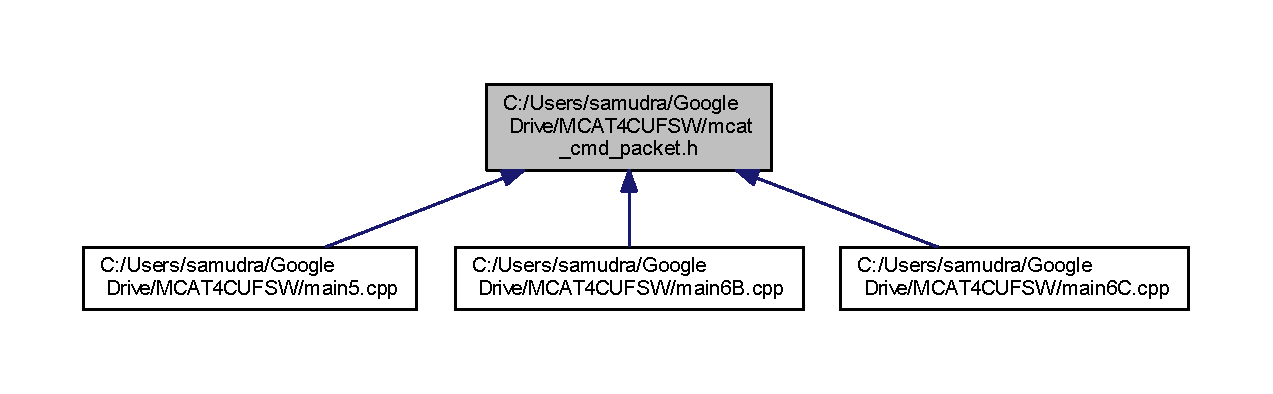
\includegraphics[width=350pt]{mcat__cmd__packet_8h__dep__incl}
\end{center}
\end{figure}
\subsection*{Macros}
\begin{DoxyCompactItemize}
\item 
\#define \hyperlink{mcat__cmd__packet_8h_ab8f39bdd707f547d924f891e63f172ee}{L\+E\+N\+\_\+\+M\+C\+A\+T\+\_\+\+C\+M\+D\+\_\+\+P\+A\+C\+K\+E\+T}~45
\item 
\#define \hyperlink{mcat__cmd__packet_8h_a4f46e7192ca001e2e6db1be75039f0ce}{L\+E\+N\+\_\+\+C\+M\+D\+\_\+\+B\+L\+O\+C\+K\+\_\+\+G}~2
\item 
\#define \hyperlink{mcat__cmd__packet_8h_a33540fa5267c548d43da04870a9ac8a0}{L\+E\+N\+\_\+\+M\+C\+A\+T\+\_\+\+C\+M\+D\+\_\+\+P\+A\+C\+K\+E\+T\+\_\+\+V\+E\+R\+S\+I\+O\+N}~2
\item 
\#define \hyperlink{mcat__cmd__packet_8h_a6b216880f6b671760c2e8baafde54b30}{M\+C\+A\+T\+\_\+\+C\+M\+D\+\_\+\+P\+A\+C\+K\+E\+T\+\_\+\+V\+E\+R\+S\+I\+O\+N}~\char`\"{}1\+B\char`\"{}
\item 
\#define \hyperlink{mcat__cmd__packet_8h_aef1ac82314f9d838f58fa6b345e76982}{M\+C\+A\+T\+\_\+\+C\+M\+D\+\_\+\+P\+A\+C\+K\+E\+T\+\_\+\+V\+E\+R\+S\+I\+O\+N\+\_\+1\+B}
\item 
\#define \hyperlink{mcat__cmd__packet_8h_a0ad2afb22413c548e9d3db6054fc005a}{L\+E\+N\+\_\+\+C\+M\+D\+\_\+\+B\+L\+O\+C\+K\+\_\+\+C\+U}~3
\item 
\#define \hyperlink{mcat__cmd__packet_8h_aaa043aacb7e6418b5e86cd6efd6852f5}{L\+E\+N\+\_\+\+C\+M\+D\+\_\+\+B\+L\+O\+C\+K\+\_\+\+C\+U\+\_\+\+M\+O\+D\+E}~3
\item 
\#define \hyperlink{mcat__cmd__packet_8h_a2f6ba47c9e2ec0f6cbdc5917fa9380ec}{M\+O\+D\+E\+\_\+\+C\+H\+A\+N\+G\+E\+\_\+\+T\+O\+\_\+\+I\+D\+L\+E}~\char`\"{}I\+D\+L\char`\"{}
\item 
\#define \hyperlink{mcat__cmd__packet_8h_ac8626c3e2d8ee55d1faa67de3294de79}{M\+O\+D\+E\+\_\+\+C\+H\+A\+N\+G\+E\+\_\+\+T\+O\+\_\+\+S\+T\+A\+N\+D\+B\+Y}~\char`\"{}S\+B\+Y\char`\"{}
\item 
\#define \hyperlink{mcat__cmd__packet_8h_a0a853095c5403044f35e770ad72812f5}{M\+O\+D\+E\+\_\+\+C\+H\+A\+N\+G\+E\+\_\+\+T\+O\+\_\+\+R\+U\+N}~\char`\"{}R\+U\+N\char`\"{}
\item 
\#define \hyperlink{mcat__cmd__packet_8h_a422df55215369fb47912cb027bd897ec}{M\+O\+D\+E\+\_\+\+C\+H\+A\+N\+G\+E\+\_\+\+T\+O\+\_\+\+F\+I\+R\+E}~\char`\"{}F\+I\+R\char`\"{}
\item 
\#define \hyperlink{mcat__cmd__packet_8h_ab43b33a60fd3f9c8c9ac1dbb82e606b9}{D\+E\+F\+\_\+\+C\+M\+D\+\_\+\+M\+O\+D\+E}~\char`\"{}I\+D\+L\char`\"{}
\item 
\#define \hyperlink{mcat__cmd__packet_8h_a0bc2274e464d562d7a52377caa2f0447}{L\+E\+N\+\_\+\+C\+M\+D\+\_\+\+B\+L\+O\+C\+K\+\_\+\+I\+P\+D}~36
\item 
\#define \hyperlink{mcat__cmd__packet_8h_a83f0d7503c6a1ecee80fa2714af08300}{L\+E\+N\+\_\+\+C\+M\+D\+\_\+\+B\+L\+O\+C\+K\+\_\+\+I\+P\+D\+\_\+\+T\+P1}~3
\item 
\#define \hyperlink{mcat__cmd__packet_8h_a5c18a0e5c855aded925219746a644788}{L\+E\+N\+\_\+\+C\+M\+D\+\_\+\+B\+L\+O\+C\+K\+\_\+\+I\+P\+D\+\_\+\+P\+C\+H1}~6
\item 
\#define \hyperlink{mcat__cmd__packet_8h_af4b46fbee704a1f9c89a6f7dd554da9b}{L\+E\+N\+\_\+\+C\+M\+D\+\_\+\+B\+L\+O\+C\+K\+\_\+\+I\+P\+D\+\_\+\+T\+P2}~3
\item 
\#define \hyperlink{mcat__cmd__packet_8h_a9d056d546abca68f8f230fcd55e5d8f1}{L\+E\+N\+\_\+\+C\+M\+D\+\_\+\+B\+L\+O\+C\+K\+\_\+\+I\+P\+D\+\_\+\+P\+C\+H2}~6
\item 
\#define \hyperlink{mcat__cmd__packet_8h_acfcf451fcced1822578bae3e5f4a2098}{L\+E\+N\+\_\+\+C\+M\+D\+\_\+\+B\+L\+O\+C\+K\+\_\+\+I\+P\+D\+\_\+\+T\+P3}~3
\item 
\#define \hyperlink{mcat__cmd__packet_8h_ac862ececdc01e89f66afbd6990540081}{L\+E\+N\+\_\+\+C\+M\+D\+\_\+\+B\+L\+O\+C\+K\+\_\+\+I\+P\+D\+\_\+\+P\+C\+H3}~6
\item 
\#define \hyperlink{mcat__cmd__packet_8h_a588a6e14078e1ba84418b990c3950a1b}{L\+E\+N\+\_\+\+C\+M\+D\+\_\+\+B\+L\+O\+C\+K\+\_\+\+I\+P\+D\+\_\+\+T\+P4}~3
\item 
\#define \hyperlink{mcat__cmd__packet_8h_a6392ca1cb2c6f4b3b9b10d2b51571377}{L\+E\+N\+\_\+\+C\+M\+D\+\_\+\+B\+L\+O\+C\+K\+\_\+\+I\+P\+D\+\_\+\+P\+C\+H4}~6
\item 
\#define \hyperlink{mcat__cmd__packet_8h_a3907bc25be720c6c2dc8d305f2f0ce9a}{D\+E\+F\+\_\+\+C\+M\+D\+\_\+\+T\+P1}~\char`\"{}00\+A\char`\"{}
\item 
\#define \hyperlink{mcat__cmd__packet_8h_aacc9d18fbbb72a4e93ad2f6881cd1a2e}{D\+E\+F\+\_\+\+C\+M\+D\+\_\+\+T\+P2}~\char`\"{}00\+A\char`\"{}
\item 
\#define \hyperlink{mcat__cmd__packet_8h_a75af00a18dea68953dad24691e1d0194}{D\+E\+F\+\_\+\+C\+M\+D\+\_\+\+T\+P3}~\char`\"{}00\+A\char`\"{}
\item 
\#define \hyperlink{mcat__cmd__packet_8h_ac41553a9799a317dc67dfc21cbb513f4}{D\+E\+F\+\_\+\+C\+M\+D\+\_\+\+T\+P4}~\char`\"{}00\+A\char`\"{}
\item 
\#define \hyperlink{mcat__cmd__packet_8h_ae3bd8145adc3b107ebf5ef028df60910}{D\+E\+F\+\_\+\+P\+C\+H1}~\char`\"{}00001\+E\char`\"{}
\item 
\#define \hyperlink{mcat__cmd__packet_8h_af14e1e6c93942e8bba3091614c17cf51}{D\+E\+F\+\_\+\+P\+C\+H2}~\char`\"{}00001\+E\char`\"{}
\item 
\#define \hyperlink{mcat__cmd__packet_8h_a4ba60c56fdf9af0a27f94d3221a45960}{D\+E\+F\+\_\+\+P\+C\+H3}~\char`\"{}00001\+E\char`\"{}
\item 
\#define \hyperlink{mcat__cmd__packet_8h_a3c8e2f43bb032d07d325abd3a89b9549}{D\+E\+F\+\_\+\+P\+C\+H4}~\char`\"{}00001\+E\char`\"{}
\item 
\#define \hyperlink{mcat__cmd__packet_8h_add545594be84723ab5cdc8e71487894e}{L\+E\+N\+\_\+\+C\+M\+D\+\_\+\+B\+L\+O\+C\+K\+\_\+\+P\+P\+U}~4
\item 
\#define \hyperlink{mcat__cmd__packet_8h_abeb144c125e898ffab17b0318396dbd6}{L\+E\+N\+\_\+\+C\+M\+D\+\_\+\+B\+L\+O\+C\+K\+\_\+\+P\+P\+U\+\_\+\+P18\+H1}~1
\item 
\#define \hyperlink{mcat__cmd__packet_8h_ab75767ea34c94ff6e0efc005519a4a74}{L\+E\+N\+\_\+\+C\+M\+D\+\_\+\+B\+L\+O\+C\+K\+\_\+\+P\+P\+U\+\_\+\+P18\+H2}~1
\item 
\#define \hyperlink{mcat__cmd__packet_8h_a59e2e3b0ba284c786c23ef4981284daa}{L\+E\+N\+\_\+\+C\+M\+D\+\_\+\+B\+L\+O\+C\+K\+\_\+\+P\+P\+U\+\_\+\+P18\+H3}~1
\item 
\#define \hyperlink{mcat__cmd__packet_8h_ac9458383c33e487f289442670129ea3c}{L\+E\+N\+\_\+\+C\+M\+D\+\_\+\+B\+L\+O\+C\+K\+\_\+\+P\+P\+U\+\_\+\+P18\+H4}~1
\item 
\#define \hyperlink{mcat__cmd__packet_8h_aa33a995f0675176ac17a5176ec226f6d}{D\+E\+F\+\_\+\+C\+M\+D\+\_\+\+P18\+H1}~\char`\"{}N\char`\"{}
\item 
\#define \hyperlink{mcat__cmd__packet_8h_a3dea2fd9ae0dd0e74ba2cb5d6e8fc9a4}{D\+E\+F\+\_\+\+C\+M\+D\+\_\+\+P18\+H2}~\char`\"{}N\char`\"{}
\item 
\#define \hyperlink{mcat__cmd__packet_8h_aa3bd948a7524221b8de9a3a75c484cdc}{D\+E\+F\+\_\+\+C\+M\+D\+\_\+\+P18\+H3}~\char`\"{}N\char`\"{}
\item 
\#define \hyperlink{mcat__cmd__packet_8h_a78b6f1ebd504c7f94aa26e8ee490b4b9}{D\+E\+F\+\_\+\+C\+M\+D\+\_\+\+P18\+H4}~\char`\"{}N\char`\"{}
\end{DoxyCompactItemize}


\subsection{Macro Definition Documentation}
\hypertarget{mcat__cmd__packet_8h_ab43b33a60fd3f9c8c9ac1dbb82e606b9}{}\index{mcat\+\_\+cmd\+\_\+packet.\+h@{mcat\+\_\+cmd\+\_\+packet.\+h}!D\+E\+F\+\_\+\+C\+M\+D\+\_\+\+M\+O\+D\+E@{D\+E\+F\+\_\+\+C\+M\+D\+\_\+\+M\+O\+D\+E}}
\index{D\+E\+F\+\_\+\+C\+M\+D\+\_\+\+M\+O\+D\+E@{D\+E\+F\+\_\+\+C\+M\+D\+\_\+\+M\+O\+D\+E}!mcat\+\_\+cmd\+\_\+packet.\+h@{mcat\+\_\+cmd\+\_\+packet.\+h}}
\subsubsection[{D\+E\+F\+\_\+\+C\+M\+D\+\_\+\+M\+O\+D\+E}]{\setlength{\rightskip}{0pt plus 5cm}\#define D\+E\+F\+\_\+\+C\+M\+D\+\_\+\+M\+O\+D\+E~\char`\"{}I\+D\+L\char`\"{}}\label{mcat__cmd__packet_8h_ab43b33a60fd3f9c8c9ac1dbb82e606b9}


Definition at line 38 of file mcat\+\_\+cmd\+\_\+packet.\+h.

\hypertarget{mcat__cmd__packet_8h_aa33a995f0675176ac17a5176ec226f6d}{}\index{mcat\+\_\+cmd\+\_\+packet.\+h@{mcat\+\_\+cmd\+\_\+packet.\+h}!D\+E\+F\+\_\+\+C\+M\+D\+\_\+\+P18\+H1@{D\+E\+F\+\_\+\+C\+M\+D\+\_\+\+P18\+H1}}
\index{D\+E\+F\+\_\+\+C\+M\+D\+\_\+\+P18\+H1@{D\+E\+F\+\_\+\+C\+M\+D\+\_\+\+P18\+H1}!mcat\+\_\+cmd\+\_\+packet.\+h@{mcat\+\_\+cmd\+\_\+packet.\+h}}
\subsubsection[{D\+E\+F\+\_\+\+C\+M\+D\+\_\+\+P18\+H1}]{\setlength{\rightskip}{0pt plus 5cm}\#define D\+E\+F\+\_\+\+C\+M\+D\+\_\+\+P18\+H1~\char`\"{}N\char`\"{}}\label{mcat__cmd__packet_8h_aa33a995f0675176ac17a5176ec226f6d}


Definition at line 77 of file mcat\+\_\+cmd\+\_\+packet.\+h.

\hypertarget{mcat__cmd__packet_8h_a3dea2fd9ae0dd0e74ba2cb5d6e8fc9a4}{}\index{mcat\+\_\+cmd\+\_\+packet.\+h@{mcat\+\_\+cmd\+\_\+packet.\+h}!D\+E\+F\+\_\+\+C\+M\+D\+\_\+\+P18\+H2@{D\+E\+F\+\_\+\+C\+M\+D\+\_\+\+P18\+H2}}
\index{D\+E\+F\+\_\+\+C\+M\+D\+\_\+\+P18\+H2@{D\+E\+F\+\_\+\+C\+M\+D\+\_\+\+P18\+H2}!mcat\+\_\+cmd\+\_\+packet.\+h@{mcat\+\_\+cmd\+\_\+packet.\+h}}
\subsubsection[{D\+E\+F\+\_\+\+C\+M\+D\+\_\+\+P18\+H2}]{\setlength{\rightskip}{0pt plus 5cm}\#define D\+E\+F\+\_\+\+C\+M\+D\+\_\+\+P18\+H2~\char`\"{}N\char`\"{}}\label{mcat__cmd__packet_8h_a3dea2fd9ae0dd0e74ba2cb5d6e8fc9a4}


Definition at line 78 of file mcat\+\_\+cmd\+\_\+packet.\+h.

\hypertarget{mcat__cmd__packet_8h_aa3bd948a7524221b8de9a3a75c484cdc}{}\index{mcat\+\_\+cmd\+\_\+packet.\+h@{mcat\+\_\+cmd\+\_\+packet.\+h}!D\+E\+F\+\_\+\+C\+M\+D\+\_\+\+P18\+H3@{D\+E\+F\+\_\+\+C\+M\+D\+\_\+\+P18\+H3}}
\index{D\+E\+F\+\_\+\+C\+M\+D\+\_\+\+P18\+H3@{D\+E\+F\+\_\+\+C\+M\+D\+\_\+\+P18\+H3}!mcat\+\_\+cmd\+\_\+packet.\+h@{mcat\+\_\+cmd\+\_\+packet.\+h}}
\subsubsection[{D\+E\+F\+\_\+\+C\+M\+D\+\_\+\+P18\+H3}]{\setlength{\rightskip}{0pt plus 5cm}\#define D\+E\+F\+\_\+\+C\+M\+D\+\_\+\+P18\+H3~\char`\"{}N\char`\"{}}\label{mcat__cmd__packet_8h_aa3bd948a7524221b8de9a3a75c484cdc}


Definition at line 79 of file mcat\+\_\+cmd\+\_\+packet.\+h.

\hypertarget{mcat__cmd__packet_8h_a78b6f1ebd504c7f94aa26e8ee490b4b9}{}\index{mcat\+\_\+cmd\+\_\+packet.\+h@{mcat\+\_\+cmd\+\_\+packet.\+h}!D\+E\+F\+\_\+\+C\+M\+D\+\_\+\+P18\+H4@{D\+E\+F\+\_\+\+C\+M\+D\+\_\+\+P18\+H4}}
\index{D\+E\+F\+\_\+\+C\+M\+D\+\_\+\+P18\+H4@{D\+E\+F\+\_\+\+C\+M\+D\+\_\+\+P18\+H4}!mcat\+\_\+cmd\+\_\+packet.\+h@{mcat\+\_\+cmd\+\_\+packet.\+h}}
\subsubsection[{D\+E\+F\+\_\+\+C\+M\+D\+\_\+\+P18\+H4}]{\setlength{\rightskip}{0pt plus 5cm}\#define D\+E\+F\+\_\+\+C\+M\+D\+\_\+\+P18\+H4~\char`\"{}N\char`\"{}}\label{mcat__cmd__packet_8h_a78b6f1ebd504c7f94aa26e8ee490b4b9}


Definition at line 80 of file mcat\+\_\+cmd\+\_\+packet.\+h.

\hypertarget{mcat__cmd__packet_8h_a3907bc25be720c6c2dc8d305f2f0ce9a}{}\index{mcat\+\_\+cmd\+\_\+packet.\+h@{mcat\+\_\+cmd\+\_\+packet.\+h}!D\+E\+F\+\_\+\+C\+M\+D\+\_\+\+T\+P1@{D\+E\+F\+\_\+\+C\+M\+D\+\_\+\+T\+P1}}
\index{D\+E\+F\+\_\+\+C\+M\+D\+\_\+\+T\+P1@{D\+E\+F\+\_\+\+C\+M\+D\+\_\+\+T\+P1}!mcat\+\_\+cmd\+\_\+packet.\+h@{mcat\+\_\+cmd\+\_\+packet.\+h}}
\subsubsection[{D\+E\+F\+\_\+\+C\+M\+D\+\_\+\+T\+P1}]{\setlength{\rightskip}{0pt plus 5cm}\#define D\+E\+F\+\_\+\+C\+M\+D\+\_\+\+T\+P1~\char`\"{}00\+A\char`\"{}}\label{mcat__cmd__packet_8h_a3907bc25be720c6c2dc8d305f2f0ce9a}


Definition at line 59 of file mcat\+\_\+cmd\+\_\+packet.\+h.

\hypertarget{mcat__cmd__packet_8h_aacc9d18fbbb72a4e93ad2f6881cd1a2e}{}\index{mcat\+\_\+cmd\+\_\+packet.\+h@{mcat\+\_\+cmd\+\_\+packet.\+h}!D\+E\+F\+\_\+\+C\+M\+D\+\_\+\+T\+P2@{D\+E\+F\+\_\+\+C\+M\+D\+\_\+\+T\+P2}}
\index{D\+E\+F\+\_\+\+C\+M\+D\+\_\+\+T\+P2@{D\+E\+F\+\_\+\+C\+M\+D\+\_\+\+T\+P2}!mcat\+\_\+cmd\+\_\+packet.\+h@{mcat\+\_\+cmd\+\_\+packet.\+h}}
\subsubsection[{D\+E\+F\+\_\+\+C\+M\+D\+\_\+\+T\+P2}]{\setlength{\rightskip}{0pt plus 5cm}\#define D\+E\+F\+\_\+\+C\+M\+D\+\_\+\+T\+P2~\char`\"{}00\+A\char`\"{}}\label{mcat__cmd__packet_8h_aacc9d18fbbb72a4e93ad2f6881cd1a2e}


Definition at line 60 of file mcat\+\_\+cmd\+\_\+packet.\+h.

\hypertarget{mcat__cmd__packet_8h_a75af00a18dea68953dad24691e1d0194}{}\index{mcat\+\_\+cmd\+\_\+packet.\+h@{mcat\+\_\+cmd\+\_\+packet.\+h}!D\+E\+F\+\_\+\+C\+M\+D\+\_\+\+T\+P3@{D\+E\+F\+\_\+\+C\+M\+D\+\_\+\+T\+P3}}
\index{D\+E\+F\+\_\+\+C\+M\+D\+\_\+\+T\+P3@{D\+E\+F\+\_\+\+C\+M\+D\+\_\+\+T\+P3}!mcat\+\_\+cmd\+\_\+packet.\+h@{mcat\+\_\+cmd\+\_\+packet.\+h}}
\subsubsection[{D\+E\+F\+\_\+\+C\+M\+D\+\_\+\+T\+P3}]{\setlength{\rightskip}{0pt plus 5cm}\#define D\+E\+F\+\_\+\+C\+M\+D\+\_\+\+T\+P3~\char`\"{}00\+A\char`\"{}}\label{mcat__cmd__packet_8h_a75af00a18dea68953dad24691e1d0194}


Definition at line 61 of file mcat\+\_\+cmd\+\_\+packet.\+h.

\hypertarget{mcat__cmd__packet_8h_ac41553a9799a317dc67dfc21cbb513f4}{}\index{mcat\+\_\+cmd\+\_\+packet.\+h@{mcat\+\_\+cmd\+\_\+packet.\+h}!D\+E\+F\+\_\+\+C\+M\+D\+\_\+\+T\+P4@{D\+E\+F\+\_\+\+C\+M\+D\+\_\+\+T\+P4}}
\index{D\+E\+F\+\_\+\+C\+M\+D\+\_\+\+T\+P4@{D\+E\+F\+\_\+\+C\+M\+D\+\_\+\+T\+P4}!mcat\+\_\+cmd\+\_\+packet.\+h@{mcat\+\_\+cmd\+\_\+packet.\+h}}
\subsubsection[{D\+E\+F\+\_\+\+C\+M\+D\+\_\+\+T\+P4}]{\setlength{\rightskip}{0pt plus 5cm}\#define D\+E\+F\+\_\+\+C\+M\+D\+\_\+\+T\+P4~\char`\"{}00\+A\char`\"{}}\label{mcat__cmd__packet_8h_ac41553a9799a317dc67dfc21cbb513f4}


Definition at line 62 of file mcat\+\_\+cmd\+\_\+packet.\+h.

\hypertarget{mcat__cmd__packet_8h_ae3bd8145adc3b107ebf5ef028df60910}{}\index{mcat\+\_\+cmd\+\_\+packet.\+h@{mcat\+\_\+cmd\+\_\+packet.\+h}!D\+E\+F\+\_\+\+P\+C\+H1@{D\+E\+F\+\_\+\+P\+C\+H1}}
\index{D\+E\+F\+\_\+\+P\+C\+H1@{D\+E\+F\+\_\+\+P\+C\+H1}!mcat\+\_\+cmd\+\_\+packet.\+h@{mcat\+\_\+cmd\+\_\+packet.\+h}}
\subsubsection[{D\+E\+F\+\_\+\+P\+C\+H1}]{\setlength{\rightskip}{0pt plus 5cm}\#define D\+E\+F\+\_\+\+P\+C\+H1~\char`\"{}00001\+E\char`\"{}}\label{mcat__cmd__packet_8h_ae3bd8145adc3b107ebf5ef028df60910}


Definition at line 63 of file mcat\+\_\+cmd\+\_\+packet.\+h.

\hypertarget{mcat__cmd__packet_8h_af14e1e6c93942e8bba3091614c17cf51}{}\index{mcat\+\_\+cmd\+\_\+packet.\+h@{mcat\+\_\+cmd\+\_\+packet.\+h}!D\+E\+F\+\_\+\+P\+C\+H2@{D\+E\+F\+\_\+\+P\+C\+H2}}
\index{D\+E\+F\+\_\+\+P\+C\+H2@{D\+E\+F\+\_\+\+P\+C\+H2}!mcat\+\_\+cmd\+\_\+packet.\+h@{mcat\+\_\+cmd\+\_\+packet.\+h}}
\subsubsection[{D\+E\+F\+\_\+\+P\+C\+H2}]{\setlength{\rightskip}{0pt plus 5cm}\#define D\+E\+F\+\_\+\+P\+C\+H2~\char`\"{}00001\+E\char`\"{}}\label{mcat__cmd__packet_8h_af14e1e6c93942e8bba3091614c17cf51}


Definition at line 64 of file mcat\+\_\+cmd\+\_\+packet.\+h.

\hypertarget{mcat__cmd__packet_8h_a4ba60c56fdf9af0a27f94d3221a45960}{}\index{mcat\+\_\+cmd\+\_\+packet.\+h@{mcat\+\_\+cmd\+\_\+packet.\+h}!D\+E\+F\+\_\+\+P\+C\+H3@{D\+E\+F\+\_\+\+P\+C\+H3}}
\index{D\+E\+F\+\_\+\+P\+C\+H3@{D\+E\+F\+\_\+\+P\+C\+H3}!mcat\+\_\+cmd\+\_\+packet.\+h@{mcat\+\_\+cmd\+\_\+packet.\+h}}
\subsubsection[{D\+E\+F\+\_\+\+P\+C\+H3}]{\setlength{\rightskip}{0pt plus 5cm}\#define D\+E\+F\+\_\+\+P\+C\+H3~\char`\"{}00001\+E\char`\"{}}\label{mcat__cmd__packet_8h_a4ba60c56fdf9af0a27f94d3221a45960}


Definition at line 65 of file mcat\+\_\+cmd\+\_\+packet.\+h.

\hypertarget{mcat__cmd__packet_8h_a3c8e2f43bb032d07d325abd3a89b9549}{}\index{mcat\+\_\+cmd\+\_\+packet.\+h@{mcat\+\_\+cmd\+\_\+packet.\+h}!D\+E\+F\+\_\+\+P\+C\+H4@{D\+E\+F\+\_\+\+P\+C\+H4}}
\index{D\+E\+F\+\_\+\+P\+C\+H4@{D\+E\+F\+\_\+\+P\+C\+H4}!mcat\+\_\+cmd\+\_\+packet.\+h@{mcat\+\_\+cmd\+\_\+packet.\+h}}
\subsubsection[{D\+E\+F\+\_\+\+P\+C\+H4}]{\setlength{\rightskip}{0pt plus 5cm}\#define D\+E\+F\+\_\+\+P\+C\+H4~\char`\"{}00001\+E\char`\"{}}\label{mcat__cmd__packet_8h_a3c8e2f43bb032d07d325abd3a89b9549}


Definition at line 66 of file mcat\+\_\+cmd\+\_\+packet.\+h.

\hypertarget{mcat__cmd__packet_8h_a0ad2afb22413c548e9d3db6054fc005a}{}\index{mcat\+\_\+cmd\+\_\+packet.\+h@{mcat\+\_\+cmd\+\_\+packet.\+h}!L\+E\+N\+\_\+\+C\+M\+D\+\_\+\+B\+L\+O\+C\+K\+\_\+\+C\+U@{L\+E\+N\+\_\+\+C\+M\+D\+\_\+\+B\+L\+O\+C\+K\+\_\+\+C\+U}}
\index{L\+E\+N\+\_\+\+C\+M\+D\+\_\+\+B\+L\+O\+C\+K\+\_\+\+C\+U@{L\+E\+N\+\_\+\+C\+M\+D\+\_\+\+B\+L\+O\+C\+K\+\_\+\+C\+U}!mcat\+\_\+cmd\+\_\+packet.\+h@{mcat\+\_\+cmd\+\_\+packet.\+h}}
\subsubsection[{L\+E\+N\+\_\+\+C\+M\+D\+\_\+\+B\+L\+O\+C\+K\+\_\+\+C\+U}]{\setlength{\rightskip}{0pt plus 5cm}\#define L\+E\+N\+\_\+\+C\+M\+D\+\_\+\+B\+L\+O\+C\+K\+\_\+\+C\+U~3}\label{mcat__cmd__packet_8h_a0ad2afb22413c548e9d3db6054fc005a}


Definition at line 30 of file mcat\+\_\+cmd\+\_\+packet.\+h.

\hypertarget{mcat__cmd__packet_8h_aaa043aacb7e6418b5e86cd6efd6852f5}{}\index{mcat\+\_\+cmd\+\_\+packet.\+h@{mcat\+\_\+cmd\+\_\+packet.\+h}!L\+E\+N\+\_\+\+C\+M\+D\+\_\+\+B\+L\+O\+C\+K\+\_\+\+C\+U\+\_\+\+M\+O\+D\+E@{L\+E\+N\+\_\+\+C\+M\+D\+\_\+\+B\+L\+O\+C\+K\+\_\+\+C\+U\+\_\+\+M\+O\+D\+E}}
\index{L\+E\+N\+\_\+\+C\+M\+D\+\_\+\+B\+L\+O\+C\+K\+\_\+\+C\+U\+\_\+\+M\+O\+D\+E@{L\+E\+N\+\_\+\+C\+M\+D\+\_\+\+B\+L\+O\+C\+K\+\_\+\+C\+U\+\_\+\+M\+O\+D\+E}!mcat\+\_\+cmd\+\_\+packet.\+h@{mcat\+\_\+cmd\+\_\+packet.\+h}}
\subsubsection[{L\+E\+N\+\_\+\+C\+M\+D\+\_\+\+B\+L\+O\+C\+K\+\_\+\+C\+U\+\_\+\+M\+O\+D\+E}]{\setlength{\rightskip}{0pt plus 5cm}\#define L\+E\+N\+\_\+\+C\+M\+D\+\_\+\+B\+L\+O\+C\+K\+\_\+\+C\+U\+\_\+\+M\+O\+D\+E~3}\label{mcat__cmd__packet_8h_aaa043aacb7e6418b5e86cd6efd6852f5}


Definition at line 31 of file mcat\+\_\+cmd\+\_\+packet.\+h.

\hypertarget{mcat__cmd__packet_8h_a4f46e7192ca001e2e6db1be75039f0ce}{}\index{mcat\+\_\+cmd\+\_\+packet.\+h@{mcat\+\_\+cmd\+\_\+packet.\+h}!L\+E\+N\+\_\+\+C\+M\+D\+\_\+\+B\+L\+O\+C\+K\+\_\+\+G@{L\+E\+N\+\_\+\+C\+M\+D\+\_\+\+B\+L\+O\+C\+K\+\_\+\+G}}
\index{L\+E\+N\+\_\+\+C\+M\+D\+\_\+\+B\+L\+O\+C\+K\+\_\+\+G@{L\+E\+N\+\_\+\+C\+M\+D\+\_\+\+B\+L\+O\+C\+K\+\_\+\+G}!mcat\+\_\+cmd\+\_\+packet.\+h@{mcat\+\_\+cmd\+\_\+packet.\+h}}
\subsubsection[{L\+E\+N\+\_\+\+C\+M\+D\+\_\+\+B\+L\+O\+C\+K\+\_\+\+G}]{\setlength{\rightskip}{0pt plus 5cm}\#define L\+E\+N\+\_\+\+C\+M\+D\+\_\+\+B\+L\+O\+C\+K\+\_\+\+G~2}\label{mcat__cmd__packet_8h_a4f46e7192ca001e2e6db1be75039f0ce}


Definition at line 19 of file mcat\+\_\+cmd\+\_\+packet.\+h.

\hypertarget{mcat__cmd__packet_8h_a0bc2274e464d562d7a52377caa2f0447}{}\index{mcat\+\_\+cmd\+\_\+packet.\+h@{mcat\+\_\+cmd\+\_\+packet.\+h}!L\+E\+N\+\_\+\+C\+M\+D\+\_\+\+B\+L\+O\+C\+K\+\_\+\+I\+P\+D@{L\+E\+N\+\_\+\+C\+M\+D\+\_\+\+B\+L\+O\+C\+K\+\_\+\+I\+P\+D}}
\index{L\+E\+N\+\_\+\+C\+M\+D\+\_\+\+B\+L\+O\+C\+K\+\_\+\+I\+P\+D@{L\+E\+N\+\_\+\+C\+M\+D\+\_\+\+B\+L\+O\+C\+K\+\_\+\+I\+P\+D}!mcat\+\_\+cmd\+\_\+packet.\+h@{mcat\+\_\+cmd\+\_\+packet.\+h}}
\subsubsection[{L\+E\+N\+\_\+\+C\+M\+D\+\_\+\+B\+L\+O\+C\+K\+\_\+\+I\+P\+D}]{\setlength{\rightskip}{0pt plus 5cm}\#define L\+E\+N\+\_\+\+C\+M\+D\+\_\+\+B\+L\+O\+C\+K\+\_\+\+I\+P\+D~36}\label{mcat__cmd__packet_8h_a0bc2274e464d562d7a52377caa2f0447}


Definition at line 48 of file mcat\+\_\+cmd\+\_\+packet.\+h.

\hypertarget{mcat__cmd__packet_8h_a5c18a0e5c855aded925219746a644788}{}\index{mcat\+\_\+cmd\+\_\+packet.\+h@{mcat\+\_\+cmd\+\_\+packet.\+h}!L\+E\+N\+\_\+\+C\+M\+D\+\_\+\+B\+L\+O\+C\+K\+\_\+\+I\+P\+D\+\_\+\+P\+C\+H1@{L\+E\+N\+\_\+\+C\+M\+D\+\_\+\+B\+L\+O\+C\+K\+\_\+\+I\+P\+D\+\_\+\+P\+C\+H1}}
\index{L\+E\+N\+\_\+\+C\+M\+D\+\_\+\+B\+L\+O\+C\+K\+\_\+\+I\+P\+D\+\_\+\+P\+C\+H1@{L\+E\+N\+\_\+\+C\+M\+D\+\_\+\+B\+L\+O\+C\+K\+\_\+\+I\+P\+D\+\_\+\+P\+C\+H1}!mcat\+\_\+cmd\+\_\+packet.\+h@{mcat\+\_\+cmd\+\_\+packet.\+h}}
\subsubsection[{L\+E\+N\+\_\+\+C\+M\+D\+\_\+\+B\+L\+O\+C\+K\+\_\+\+I\+P\+D\+\_\+\+P\+C\+H1}]{\setlength{\rightskip}{0pt plus 5cm}\#define L\+E\+N\+\_\+\+C\+M\+D\+\_\+\+B\+L\+O\+C\+K\+\_\+\+I\+P\+D\+\_\+\+P\+C\+H1~6}\label{mcat__cmd__packet_8h_a5c18a0e5c855aded925219746a644788}


Definition at line 50 of file mcat\+\_\+cmd\+\_\+packet.\+h.

\hypertarget{mcat__cmd__packet_8h_a9d056d546abca68f8f230fcd55e5d8f1}{}\index{mcat\+\_\+cmd\+\_\+packet.\+h@{mcat\+\_\+cmd\+\_\+packet.\+h}!L\+E\+N\+\_\+\+C\+M\+D\+\_\+\+B\+L\+O\+C\+K\+\_\+\+I\+P\+D\+\_\+\+P\+C\+H2@{L\+E\+N\+\_\+\+C\+M\+D\+\_\+\+B\+L\+O\+C\+K\+\_\+\+I\+P\+D\+\_\+\+P\+C\+H2}}
\index{L\+E\+N\+\_\+\+C\+M\+D\+\_\+\+B\+L\+O\+C\+K\+\_\+\+I\+P\+D\+\_\+\+P\+C\+H2@{L\+E\+N\+\_\+\+C\+M\+D\+\_\+\+B\+L\+O\+C\+K\+\_\+\+I\+P\+D\+\_\+\+P\+C\+H2}!mcat\+\_\+cmd\+\_\+packet.\+h@{mcat\+\_\+cmd\+\_\+packet.\+h}}
\subsubsection[{L\+E\+N\+\_\+\+C\+M\+D\+\_\+\+B\+L\+O\+C\+K\+\_\+\+I\+P\+D\+\_\+\+P\+C\+H2}]{\setlength{\rightskip}{0pt plus 5cm}\#define L\+E\+N\+\_\+\+C\+M\+D\+\_\+\+B\+L\+O\+C\+K\+\_\+\+I\+P\+D\+\_\+\+P\+C\+H2~6}\label{mcat__cmd__packet_8h_a9d056d546abca68f8f230fcd55e5d8f1}


Definition at line 52 of file mcat\+\_\+cmd\+\_\+packet.\+h.

\hypertarget{mcat__cmd__packet_8h_ac862ececdc01e89f66afbd6990540081}{}\index{mcat\+\_\+cmd\+\_\+packet.\+h@{mcat\+\_\+cmd\+\_\+packet.\+h}!L\+E\+N\+\_\+\+C\+M\+D\+\_\+\+B\+L\+O\+C\+K\+\_\+\+I\+P\+D\+\_\+\+P\+C\+H3@{L\+E\+N\+\_\+\+C\+M\+D\+\_\+\+B\+L\+O\+C\+K\+\_\+\+I\+P\+D\+\_\+\+P\+C\+H3}}
\index{L\+E\+N\+\_\+\+C\+M\+D\+\_\+\+B\+L\+O\+C\+K\+\_\+\+I\+P\+D\+\_\+\+P\+C\+H3@{L\+E\+N\+\_\+\+C\+M\+D\+\_\+\+B\+L\+O\+C\+K\+\_\+\+I\+P\+D\+\_\+\+P\+C\+H3}!mcat\+\_\+cmd\+\_\+packet.\+h@{mcat\+\_\+cmd\+\_\+packet.\+h}}
\subsubsection[{L\+E\+N\+\_\+\+C\+M\+D\+\_\+\+B\+L\+O\+C\+K\+\_\+\+I\+P\+D\+\_\+\+P\+C\+H3}]{\setlength{\rightskip}{0pt plus 5cm}\#define L\+E\+N\+\_\+\+C\+M\+D\+\_\+\+B\+L\+O\+C\+K\+\_\+\+I\+P\+D\+\_\+\+P\+C\+H3~6}\label{mcat__cmd__packet_8h_ac862ececdc01e89f66afbd6990540081}


Definition at line 54 of file mcat\+\_\+cmd\+\_\+packet.\+h.

\hypertarget{mcat__cmd__packet_8h_a6392ca1cb2c6f4b3b9b10d2b51571377}{}\index{mcat\+\_\+cmd\+\_\+packet.\+h@{mcat\+\_\+cmd\+\_\+packet.\+h}!L\+E\+N\+\_\+\+C\+M\+D\+\_\+\+B\+L\+O\+C\+K\+\_\+\+I\+P\+D\+\_\+\+P\+C\+H4@{L\+E\+N\+\_\+\+C\+M\+D\+\_\+\+B\+L\+O\+C\+K\+\_\+\+I\+P\+D\+\_\+\+P\+C\+H4}}
\index{L\+E\+N\+\_\+\+C\+M\+D\+\_\+\+B\+L\+O\+C\+K\+\_\+\+I\+P\+D\+\_\+\+P\+C\+H4@{L\+E\+N\+\_\+\+C\+M\+D\+\_\+\+B\+L\+O\+C\+K\+\_\+\+I\+P\+D\+\_\+\+P\+C\+H4}!mcat\+\_\+cmd\+\_\+packet.\+h@{mcat\+\_\+cmd\+\_\+packet.\+h}}
\subsubsection[{L\+E\+N\+\_\+\+C\+M\+D\+\_\+\+B\+L\+O\+C\+K\+\_\+\+I\+P\+D\+\_\+\+P\+C\+H4}]{\setlength{\rightskip}{0pt plus 5cm}\#define L\+E\+N\+\_\+\+C\+M\+D\+\_\+\+B\+L\+O\+C\+K\+\_\+\+I\+P\+D\+\_\+\+P\+C\+H4~6}\label{mcat__cmd__packet_8h_a6392ca1cb2c6f4b3b9b10d2b51571377}


Definition at line 56 of file mcat\+\_\+cmd\+\_\+packet.\+h.

\hypertarget{mcat__cmd__packet_8h_a83f0d7503c6a1ecee80fa2714af08300}{}\index{mcat\+\_\+cmd\+\_\+packet.\+h@{mcat\+\_\+cmd\+\_\+packet.\+h}!L\+E\+N\+\_\+\+C\+M\+D\+\_\+\+B\+L\+O\+C\+K\+\_\+\+I\+P\+D\+\_\+\+T\+P1@{L\+E\+N\+\_\+\+C\+M\+D\+\_\+\+B\+L\+O\+C\+K\+\_\+\+I\+P\+D\+\_\+\+T\+P1}}
\index{L\+E\+N\+\_\+\+C\+M\+D\+\_\+\+B\+L\+O\+C\+K\+\_\+\+I\+P\+D\+\_\+\+T\+P1@{L\+E\+N\+\_\+\+C\+M\+D\+\_\+\+B\+L\+O\+C\+K\+\_\+\+I\+P\+D\+\_\+\+T\+P1}!mcat\+\_\+cmd\+\_\+packet.\+h@{mcat\+\_\+cmd\+\_\+packet.\+h}}
\subsubsection[{L\+E\+N\+\_\+\+C\+M\+D\+\_\+\+B\+L\+O\+C\+K\+\_\+\+I\+P\+D\+\_\+\+T\+P1}]{\setlength{\rightskip}{0pt plus 5cm}\#define L\+E\+N\+\_\+\+C\+M\+D\+\_\+\+B\+L\+O\+C\+K\+\_\+\+I\+P\+D\+\_\+\+T\+P1~3}\label{mcat__cmd__packet_8h_a83f0d7503c6a1ecee80fa2714af08300}


Definition at line 49 of file mcat\+\_\+cmd\+\_\+packet.\+h.

\hypertarget{mcat__cmd__packet_8h_af4b46fbee704a1f9c89a6f7dd554da9b}{}\index{mcat\+\_\+cmd\+\_\+packet.\+h@{mcat\+\_\+cmd\+\_\+packet.\+h}!L\+E\+N\+\_\+\+C\+M\+D\+\_\+\+B\+L\+O\+C\+K\+\_\+\+I\+P\+D\+\_\+\+T\+P2@{L\+E\+N\+\_\+\+C\+M\+D\+\_\+\+B\+L\+O\+C\+K\+\_\+\+I\+P\+D\+\_\+\+T\+P2}}
\index{L\+E\+N\+\_\+\+C\+M\+D\+\_\+\+B\+L\+O\+C\+K\+\_\+\+I\+P\+D\+\_\+\+T\+P2@{L\+E\+N\+\_\+\+C\+M\+D\+\_\+\+B\+L\+O\+C\+K\+\_\+\+I\+P\+D\+\_\+\+T\+P2}!mcat\+\_\+cmd\+\_\+packet.\+h@{mcat\+\_\+cmd\+\_\+packet.\+h}}
\subsubsection[{L\+E\+N\+\_\+\+C\+M\+D\+\_\+\+B\+L\+O\+C\+K\+\_\+\+I\+P\+D\+\_\+\+T\+P2}]{\setlength{\rightskip}{0pt plus 5cm}\#define L\+E\+N\+\_\+\+C\+M\+D\+\_\+\+B\+L\+O\+C\+K\+\_\+\+I\+P\+D\+\_\+\+T\+P2~3}\label{mcat__cmd__packet_8h_af4b46fbee704a1f9c89a6f7dd554da9b}


Definition at line 51 of file mcat\+\_\+cmd\+\_\+packet.\+h.

\hypertarget{mcat__cmd__packet_8h_acfcf451fcced1822578bae3e5f4a2098}{}\index{mcat\+\_\+cmd\+\_\+packet.\+h@{mcat\+\_\+cmd\+\_\+packet.\+h}!L\+E\+N\+\_\+\+C\+M\+D\+\_\+\+B\+L\+O\+C\+K\+\_\+\+I\+P\+D\+\_\+\+T\+P3@{L\+E\+N\+\_\+\+C\+M\+D\+\_\+\+B\+L\+O\+C\+K\+\_\+\+I\+P\+D\+\_\+\+T\+P3}}
\index{L\+E\+N\+\_\+\+C\+M\+D\+\_\+\+B\+L\+O\+C\+K\+\_\+\+I\+P\+D\+\_\+\+T\+P3@{L\+E\+N\+\_\+\+C\+M\+D\+\_\+\+B\+L\+O\+C\+K\+\_\+\+I\+P\+D\+\_\+\+T\+P3}!mcat\+\_\+cmd\+\_\+packet.\+h@{mcat\+\_\+cmd\+\_\+packet.\+h}}
\subsubsection[{L\+E\+N\+\_\+\+C\+M\+D\+\_\+\+B\+L\+O\+C\+K\+\_\+\+I\+P\+D\+\_\+\+T\+P3}]{\setlength{\rightskip}{0pt plus 5cm}\#define L\+E\+N\+\_\+\+C\+M\+D\+\_\+\+B\+L\+O\+C\+K\+\_\+\+I\+P\+D\+\_\+\+T\+P3~3}\label{mcat__cmd__packet_8h_acfcf451fcced1822578bae3e5f4a2098}


Definition at line 53 of file mcat\+\_\+cmd\+\_\+packet.\+h.

\hypertarget{mcat__cmd__packet_8h_a588a6e14078e1ba84418b990c3950a1b}{}\index{mcat\+\_\+cmd\+\_\+packet.\+h@{mcat\+\_\+cmd\+\_\+packet.\+h}!L\+E\+N\+\_\+\+C\+M\+D\+\_\+\+B\+L\+O\+C\+K\+\_\+\+I\+P\+D\+\_\+\+T\+P4@{L\+E\+N\+\_\+\+C\+M\+D\+\_\+\+B\+L\+O\+C\+K\+\_\+\+I\+P\+D\+\_\+\+T\+P4}}
\index{L\+E\+N\+\_\+\+C\+M\+D\+\_\+\+B\+L\+O\+C\+K\+\_\+\+I\+P\+D\+\_\+\+T\+P4@{L\+E\+N\+\_\+\+C\+M\+D\+\_\+\+B\+L\+O\+C\+K\+\_\+\+I\+P\+D\+\_\+\+T\+P4}!mcat\+\_\+cmd\+\_\+packet.\+h@{mcat\+\_\+cmd\+\_\+packet.\+h}}
\subsubsection[{L\+E\+N\+\_\+\+C\+M\+D\+\_\+\+B\+L\+O\+C\+K\+\_\+\+I\+P\+D\+\_\+\+T\+P4}]{\setlength{\rightskip}{0pt plus 5cm}\#define L\+E\+N\+\_\+\+C\+M\+D\+\_\+\+B\+L\+O\+C\+K\+\_\+\+I\+P\+D\+\_\+\+T\+P4~3}\label{mcat__cmd__packet_8h_a588a6e14078e1ba84418b990c3950a1b}


Definition at line 55 of file mcat\+\_\+cmd\+\_\+packet.\+h.

\hypertarget{mcat__cmd__packet_8h_add545594be84723ab5cdc8e71487894e}{}\index{mcat\+\_\+cmd\+\_\+packet.\+h@{mcat\+\_\+cmd\+\_\+packet.\+h}!L\+E\+N\+\_\+\+C\+M\+D\+\_\+\+B\+L\+O\+C\+K\+\_\+\+P\+P\+U@{L\+E\+N\+\_\+\+C\+M\+D\+\_\+\+B\+L\+O\+C\+K\+\_\+\+P\+P\+U}}
\index{L\+E\+N\+\_\+\+C\+M\+D\+\_\+\+B\+L\+O\+C\+K\+\_\+\+P\+P\+U@{L\+E\+N\+\_\+\+C\+M\+D\+\_\+\+B\+L\+O\+C\+K\+\_\+\+P\+P\+U}!mcat\+\_\+cmd\+\_\+packet.\+h@{mcat\+\_\+cmd\+\_\+packet.\+h}}
\subsubsection[{L\+E\+N\+\_\+\+C\+M\+D\+\_\+\+B\+L\+O\+C\+K\+\_\+\+P\+P\+U}]{\setlength{\rightskip}{0pt plus 5cm}\#define L\+E\+N\+\_\+\+C\+M\+D\+\_\+\+B\+L\+O\+C\+K\+\_\+\+P\+P\+U~4}\label{mcat__cmd__packet_8h_add545594be84723ab5cdc8e71487894e}


Definition at line 70 of file mcat\+\_\+cmd\+\_\+packet.\+h.

\hypertarget{mcat__cmd__packet_8h_abeb144c125e898ffab17b0318396dbd6}{}\index{mcat\+\_\+cmd\+\_\+packet.\+h@{mcat\+\_\+cmd\+\_\+packet.\+h}!L\+E\+N\+\_\+\+C\+M\+D\+\_\+\+B\+L\+O\+C\+K\+\_\+\+P\+P\+U\+\_\+\+P18\+H1@{L\+E\+N\+\_\+\+C\+M\+D\+\_\+\+B\+L\+O\+C\+K\+\_\+\+P\+P\+U\+\_\+\+P18\+H1}}
\index{L\+E\+N\+\_\+\+C\+M\+D\+\_\+\+B\+L\+O\+C\+K\+\_\+\+P\+P\+U\+\_\+\+P18\+H1@{L\+E\+N\+\_\+\+C\+M\+D\+\_\+\+B\+L\+O\+C\+K\+\_\+\+P\+P\+U\+\_\+\+P18\+H1}!mcat\+\_\+cmd\+\_\+packet.\+h@{mcat\+\_\+cmd\+\_\+packet.\+h}}
\subsubsection[{L\+E\+N\+\_\+\+C\+M\+D\+\_\+\+B\+L\+O\+C\+K\+\_\+\+P\+P\+U\+\_\+\+P18\+H1}]{\setlength{\rightskip}{0pt plus 5cm}\#define L\+E\+N\+\_\+\+C\+M\+D\+\_\+\+B\+L\+O\+C\+K\+\_\+\+P\+P\+U\+\_\+\+P18\+H1~1}\label{mcat__cmd__packet_8h_abeb144c125e898ffab17b0318396dbd6}


Definition at line 71 of file mcat\+\_\+cmd\+\_\+packet.\+h.

\hypertarget{mcat__cmd__packet_8h_ab75767ea34c94ff6e0efc005519a4a74}{}\index{mcat\+\_\+cmd\+\_\+packet.\+h@{mcat\+\_\+cmd\+\_\+packet.\+h}!L\+E\+N\+\_\+\+C\+M\+D\+\_\+\+B\+L\+O\+C\+K\+\_\+\+P\+P\+U\+\_\+\+P18\+H2@{L\+E\+N\+\_\+\+C\+M\+D\+\_\+\+B\+L\+O\+C\+K\+\_\+\+P\+P\+U\+\_\+\+P18\+H2}}
\index{L\+E\+N\+\_\+\+C\+M\+D\+\_\+\+B\+L\+O\+C\+K\+\_\+\+P\+P\+U\+\_\+\+P18\+H2@{L\+E\+N\+\_\+\+C\+M\+D\+\_\+\+B\+L\+O\+C\+K\+\_\+\+P\+P\+U\+\_\+\+P18\+H2}!mcat\+\_\+cmd\+\_\+packet.\+h@{mcat\+\_\+cmd\+\_\+packet.\+h}}
\subsubsection[{L\+E\+N\+\_\+\+C\+M\+D\+\_\+\+B\+L\+O\+C\+K\+\_\+\+P\+P\+U\+\_\+\+P18\+H2}]{\setlength{\rightskip}{0pt plus 5cm}\#define L\+E\+N\+\_\+\+C\+M\+D\+\_\+\+B\+L\+O\+C\+K\+\_\+\+P\+P\+U\+\_\+\+P18\+H2~1}\label{mcat__cmd__packet_8h_ab75767ea34c94ff6e0efc005519a4a74}


Definition at line 72 of file mcat\+\_\+cmd\+\_\+packet.\+h.

\hypertarget{mcat__cmd__packet_8h_a59e2e3b0ba284c786c23ef4981284daa}{}\index{mcat\+\_\+cmd\+\_\+packet.\+h@{mcat\+\_\+cmd\+\_\+packet.\+h}!L\+E\+N\+\_\+\+C\+M\+D\+\_\+\+B\+L\+O\+C\+K\+\_\+\+P\+P\+U\+\_\+\+P18\+H3@{L\+E\+N\+\_\+\+C\+M\+D\+\_\+\+B\+L\+O\+C\+K\+\_\+\+P\+P\+U\+\_\+\+P18\+H3}}
\index{L\+E\+N\+\_\+\+C\+M\+D\+\_\+\+B\+L\+O\+C\+K\+\_\+\+P\+P\+U\+\_\+\+P18\+H3@{L\+E\+N\+\_\+\+C\+M\+D\+\_\+\+B\+L\+O\+C\+K\+\_\+\+P\+P\+U\+\_\+\+P18\+H3}!mcat\+\_\+cmd\+\_\+packet.\+h@{mcat\+\_\+cmd\+\_\+packet.\+h}}
\subsubsection[{L\+E\+N\+\_\+\+C\+M\+D\+\_\+\+B\+L\+O\+C\+K\+\_\+\+P\+P\+U\+\_\+\+P18\+H3}]{\setlength{\rightskip}{0pt plus 5cm}\#define L\+E\+N\+\_\+\+C\+M\+D\+\_\+\+B\+L\+O\+C\+K\+\_\+\+P\+P\+U\+\_\+\+P18\+H3~1}\label{mcat__cmd__packet_8h_a59e2e3b0ba284c786c23ef4981284daa}


Definition at line 73 of file mcat\+\_\+cmd\+\_\+packet.\+h.

\hypertarget{mcat__cmd__packet_8h_ac9458383c33e487f289442670129ea3c}{}\index{mcat\+\_\+cmd\+\_\+packet.\+h@{mcat\+\_\+cmd\+\_\+packet.\+h}!L\+E\+N\+\_\+\+C\+M\+D\+\_\+\+B\+L\+O\+C\+K\+\_\+\+P\+P\+U\+\_\+\+P18\+H4@{L\+E\+N\+\_\+\+C\+M\+D\+\_\+\+B\+L\+O\+C\+K\+\_\+\+P\+P\+U\+\_\+\+P18\+H4}}
\index{L\+E\+N\+\_\+\+C\+M\+D\+\_\+\+B\+L\+O\+C\+K\+\_\+\+P\+P\+U\+\_\+\+P18\+H4@{L\+E\+N\+\_\+\+C\+M\+D\+\_\+\+B\+L\+O\+C\+K\+\_\+\+P\+P\+U\+\_\+\+P18\+H4}!mcat\+\_\+cmd\+\_\+packet.\+h@{mcat\+\_\+cmd\+\_\+packet.\+h}}
\subsubsection[{L\+E\+N\+\_\+\+C\+M\+D\+\_\+\+B\+L\+O\+C\+K\+\_\+\+P\+P\+U\+\_\+\+P18\+H4}]{\setlength{\rightskip}{0pt plus 5cm}\#define L\+E\+N\+\_\+\+C\+M\+D\+\_\+\+B\+L\+O\+C\+K\+\_\+\+P\+P\+U\+\_\+\+P18\+H4~1}\label{mcat__cmd__packet_8h_ac9458383c33e487f289442670129ea3c}


Definition at line 74 of file mcat\+\_\+cmd\+\_\+packet.\+h.

\hypertarget{mcat__cmd__packet_8h_ab8f39bdd707f547d924f891e63f172ee}{}\index{mcat\+\_\+cmd\+\_\+packet.\+h@{mcat\+\_\+cmd\+\_\+packet.\+h}!L\+E\+N\+\_\+\+M\+C\+A\+T\+\_\+\+C\+M\+D\+\_\+\+P\+A\+C\+K\+E\+T@{L\+E\+N\+\_\+\+M\+C\+A\+T\+\_\+\+C\+M\+D\+\_\+\+P\+A\+C\+K\+E\+T}}
\index{L\+E\+N\+\_\+\+M\+C\+A\+T\+\_\+\+C\+M\+D\+\_\+\+P\+A\+C\+K\+E\+T@{L\+E\+N\+\_\+\+M\+C\+A\+T\+\_\+\+C\+M\+D\+\_\+\+P\+A\+C\+K\+E\+T}!mcat\+\_\+cmd\+\_\+packet.\+h@{mcat\+\_\+cmd\+\_\+packet.\+h}}
\subsubsection[{L\+E\+N\+\_\+\+M\+C\+A\+T\+\_\+\+C\+M\+D\+\_\+\+P\+A\+C\+K\+E\+T}]{\setlength{\rightskip}{0pt plus 5cm}\#define L\+E\+N\+\_\+\+M\+C\+A\+T\+\_\+\+C\+M\+D\+\_\+\+P\+A\+C\+K\+E\+T~45}\label{mcat__cmd__packet_8h_ab8f39bdd707f547d924f891e63f172ee}


Definition at line 15 of file mcat\+\_\+cmd\+\_\+packet.\+h.

\hypertarget{mcat__cmd__packet_8h_a33540fa5267c548d43da04870a9ac8a0}{}\index{mcat\+\_\+cmd\+\_\+packet.\+h@{mcat\+\_\+cmd\+\_\+packet.\+h}!L\+E\+N\+\_\+\+M\+C\+A\+T\+\_\+\+C\+M\+D\+\_\+\+P\+A\+C\+K\+E\+T\+\_\+\+V\+E\+R\+S\+I\+O\+N@{L\+E\+N\+\_\+\+M\+C\+A\+T\+\_\+\+C\+M\+D\+\_\+\+P\+A\+C\+K\+E\+T\+\_\+\+V\+E\+R\+S\+I\+O\+N}}
\index{L\+E\+N\+\_\+\+M\+C\+A\+T\+\_\+\+C\+M\+D\+\_\+\+P\+A\+C\+K\+E\+T\+\_\+\+V\+E\+R\+S\+I\+O\+N@{L\+E\+N\+\_\+\+M\+C\+A\+T\+\_\+\+C\+M\+D\+\_\+\+P\+A\+C\+K\+E\+T\+\_\+\+V\+E\+R\+S\+I\+O\+N}!mcat\+\_\+cmd\+\_\+packet.\+h@{mcat\+\_\+cmd\+\_\+packet.\+h}}
\subsubsection[{L\+E\+N\+\_\+\+M\+C\+A\+T\+\_\+\+C\+M\+D\+\_\+\+P\+A\+C\+K\+E\+T\+\_\+\+V\+E\+R\+S\+I\+O\+N}]{\setlength{\rightskip}{0pt plus 5cm}\#define L\+E\+N\+\_\+\+M\+C\+A\+T\+\_\+\+C\+M\+D\+\_\+\+P\+A\+C\+K\+E\+T\+\_\+\+V\+E\+R\+S\+I\+O\+N~2}\label{mcat__cmd__packet_8h_a33540fa5267c548d43da04870a9ac8a0}


Definition at line 20 of file mcat\+\_\+cmd\+\_\+packet.\+h.

\hypertarget{mcat__cmd__packet_8h_a6b216880f6b671760c2e8baafde54b30}{}\index{mcat\+\_\+cmd\+\_\+packet.\+h@{mcat\+\_\+cmd\+\_\+packet.\+h}!M\+C\+A\+T\+\_\+\+C\+M\+D\+\_\+\+P\+A\+C\+K\+E\+T\+\_\+\+V\+E\+R\+S\+I\+O\+N@{M\+C\+A\+T\+\_\+\+C\+M\+D\+\_\+\+P\+A\+C\+K\+E\+T\+\_\+\+V\+E\+R\+S\+I\+O\+N}}
\index{M\+C\+A\+T\+\_\+\+C\+M\+D\+\_\+\+P\+A\+C\+K\+E\+T\+\_\+\+V\+E\+R\+S\+I\+O\+N@{M\+C\+A\+T\+\_\+\+C\+M\+D\+\_\+\+P\+A\+C\+K\+E\+T\+\_\+\+V\+E\+R\+S\+I\+O\+N}!mcat\+\_\+cmd\+\_\+packet.\+h@{mcat\+\_\+cmd\+\_\+packet.\+h}}
\subsubsection[{M\+C\+A\+T\+\_\+\+C\+M\+D\+\_\+\+P\+A\+C\+K\+E\+T\+\_\+\+V\+E\+R\+S\+I\+O\+N}]{\setlength{\rightskip}{0pt plus 5cm}\#define M\+C\+A\+T\+\_\+\+C\+M\+D\+\_\+\+P\+A\+C\+K\+E\+T\+\_\+\+V\+E\+R\+S\+I\+O\+N~\char`\"{}1\+B\char`\"{}}\label{mcat__cmd__packet_8h_a6b216880f6b671760c2e8baafde54b30}


Definition at line 22 of file mcat\+\_\+cmd\+\_\+packet.\+h.

\hypertarget{mcat__cmd__packet_8h_aef1ac82314f9d838f58fa6b345e76982}{}\index{mcat\+\_\+cmd\+\_\+packet.\+h@{mcat\+\_\+cmd\+\_\+packet.\+h}!M\+C\+A\+T\+\_\+\+C\+M\+D\+\_\+\+P\+A\+C\+K\+E\+T\+\_\+\+V\+E\+R\+S\+I\+O\+N\+\_\+1\+B@{M\+C\+A\+T\+\_\+\+C\+M\+D\+\_\+\+P\+A\+C\+K\+E\+T\+\_\+\+V\+E\+R\+S\+I\+O\+N\+\_\+1\+B}}
\index{M\+C\+A\+T\+\_\+\+C\+M\+D\+\_\+\+P\+A\+C\+K\+E\+T\+\_\+\+V\+E\+R\+S\+I\+O\+N\+\_\+1\+B@{M\+C\+A\+T\+\_\+\+C\+M\+D\+\_\+\+P\+A\+C\+K\+E\+T\+\_\+\+V\+E\+R\+S\+I\+O\+N\+\_\+1\+B}!mcat\+\_\+cmd\+\_\+packet.\+h@{mcat\+\_\+cmd\+\_\+packet.\+h}}
\subsubsection[{M\+C\+A\+T\+\_\+\+C\+M\+D\+\_\+\+P\+A\+C\+K\+E\+T\+\_\+\+V\+E\+R\+S\+I\+O\+N\+\_\+1\+B}]{\setlength{\rightskip}{0pt plus 5cm}\#define M\+C\+A\+T\+\_\+\+C\+M\+D\+\_\+\+P\+A\+C\+K\+E\+T\+\_\+\+V\+E\+R\+S\+I\+O\+N\+\_\+1\+B}\label{mcat__cmd__packet_8h_aef1ac82314f9d838f58fa6b345e76982}


Definition at line 23 of file mcat\+\_\+cmd\+\_\+packet.\+h.

\hypertarget{mcat__cmd__packet_8h_a422df55215369fb47912cb027bd897ec}{}\index{mcat\+\_\+cmd\+\_\+packet.\+h@{mcat\+\_\+cmd\+\_\+packet.\+h}!M\+O\+D\+E\+\_\+\+C\+H\+A\+N\+G\+E\+\_\+\+T\+O\+\_\+\+F\+I\+R\+E@{M\+O\+D\+E\+\_\+\+C\+H\+A\+N\+G\+E\+\_\+\+T\+O\+\_\+\+F\+I\+R\+E}}
\index{M\+O\+D\+E\+\_\+\+C\+H\+A\+N\+G\+E\+\_\+\+T\+O\+\_\+\+F\+I\+R\+E@{M\+O\+D\+E\+\_\+\+C\+H\+A\+N\+G\+E\+\_\+\+T\+O\+\_\+\+F\+I\+R\+E}!mcat\+\_\+cmd\+\_\+packet.\+h@{mcat\+\_\+cmd\+\_\+packet.\+h}}
\subsubsection[{M\+O\+D\+E\+\_\+\+C\+H\+A\+N\+G\+E\+\_\+\+T\+O\+\_\+\+F\+I\+R\+E}]{\setlength{\rightskip}{0pt plus 5cm}\#define M\+O\+D\+E\+\_\+\+C\+H\+A\+N\+G\+E\+\_\+\+T\+O\+\_\+\+F\+I\+R\+E~\char`\"{}F\+I\+R\char`\"{}}\label{mcat__cmd__packet_8h_a422df55215369fb47912cb027bd897ec}


Definition at line 36 of file mcat\+\_\+cmd\+\_\+packet.\+h.

\hypertarget{mcat__cmd__packet_8h_a2f6ba47c9e2ec0f6cbdc5917fa9380ec}{}\index{mcat\+\_\+cmd\+\_\+packet.\+h@{mcat\+\_\+cmd\+\_\+packet.\+h}!M\+O\+D\+E\+\_\+\+C\+H\+A\+N\+G\+E\+\_\+\+T\+O\+\_\+\+I\+D\+L\+E@{M\+O\+D\+E\+\_\+\+C\+H\+A\+N\+G\+E\+\_\+\+T\+O\+\_\+\+I\+D\+L\+E}}
\index{M\+O\+D\+E\+\_\+\+C\+H\+A\+N\+G\+E\+\_\+\+T\+O\+\_\+\+I\+D\+L\+E@{M\+O\+D\+E\+\_\+\+C\+H\+A\+N\+G\+E\+\_\+\+T\+O\+\_\+\+I\+D\+L\+E}!mcat\+\_\+cmd\+\_\+packet.\+h@{mcat\+\_\+cmd\+\_\+packet.\+h}}
\subsubsection[{M\+O\+D\+E\+\_\+\+C\+H\+A\+N\+G\+E\+\_\+\+T\+O\+\_\+\+I\+D\+L\+E}]{\setlength{\rightskip}{0pt plus 5cm}\#define M\+O\+D\+E\+\_\+\+C\+H\+A\+N\+G\+E\+\_\+\+T\+O\+\_\+\+I\+D\+L\+E~\char`\"{}I\+D\+L\char`\"{}}\label{mcat__cmd__packet_8h_a2f6ba47c9e2ec0f6cbdc5917fa9380ec}


Definition at line 33 of file mcat\+\_\+cmd\+\_\+packet.\+h.

\hypertarget{mcat__cmd__packet_8h_a0a853095c5403044f35e770ad72812f5}{}\index{mcat\+\_\+cmd\+\_\+packet.\+h@{mcat\+\_\+cmd\+\_\+packet.\+h}!M\+O\+D\+E\+\_\+\+C\+H\+A\+N\+G\+E\+\_\+\+T\+O\+\_\+\+R\+U\+N@{M\+O\+D\+E\+\_\+\+C\+H\+A\+N\+G\+E\+\_\+\+T\+O\+\_\+\+R\+U\+N}}
\index{M\+O\+D\+E\+\_\+\+C\+H\+A\+N\+G\+E\+\_\+\+T\+O\+\_\+\+R\+U\+N@{M\+O\+D\+E\+\_\+\+C\+H\+A\+N\+G\+E\+\_\+\+T\+O\+\_\+\+R\+U\+N}!mcat\+\_\+cmd\+\_\+packet.\+h@{mcat\+\_\+cmd\+\_\+packet.\+h}}
\subsubsection[{M\+O\+D\+E\+\_\+\+C\+H\+A\+N\+G\+E\+\_\+\+T\+O\+\_\+\+R\+U\+N}]{\setlength{\rightskip}{0pt plus 5cm}\#define M\+O\+D\+E\+\_\+\+C\+H\+A\+N\+G\+E\+\_\+\+T\+O\+\_\+\+R\+U\+N~\char`\"{}R\+U\+N\char`\"{}}\label{mcat__cmd__packet_8h_a0a853095c5403044f35e770ad72812f5}


Definition at line 35 of file mcat\+\_\+cmd\+\_\+packet.\+h.

\hypertarget{mcat__cmd__packet_8h_ac8626c3e2d8ee55d1faa67de3294de79}{}\index{mcat\+\_\+cmd\+\_\+packet.\+h@{mcat\+\_\+cmd\+\_\+packet.\+h}!M\+O\+D\+E\+\_\+\+C\+H\+A\+N\+G\+E\+\_\+\+T\+O\+\_\+\+S\+T\+A\+N\+D\+B\+Y@{M\+O\+D\+E\+\_\+\+C\+H\+A\+N\+G\+E\+\_\+\+T\+O\+\_\+\+S\+T\+A\+N\+D\+B\+Y}}
\index{M\+O\+D\+E\+\_\+\+C\+H\+A\+N\+G\+E\+\_\+\+T\+O\+\_\+\+S\+T\+A\+N\+D\+B\+Y@{M\+O\+D\+E\+\_\+\+C\+H\+A\+N\+G\+E\+\_\+\+T\+O\+\_\+\+S\+T\+A\+N\+D\+B\+Y}!mcat\+\_\+cmd\+\_\+packet.\+h@{mcat\+\_\+cmd\+\_\+packet.\+h}}
\subsubsection[{M\+O\+D\+E\+\_\+\+C\+H\+A\+N\+G\+E\+\_\+\+T\+O\+\_\+\+S\+T\+A\+N\+D\+B\+Y}]{\setlength{\rightskip}{0pt plus 5cm}\#define M\+O\+D\+E\+\_\+\+C\+H\+A\+N\+G\+E\+\_\+\+T\+O\+\_\+\+S\+T\+A\+N\+D\+B\+Y~\char`\"{}S\+B\+Y\char`\"{}}\label{mcat__cmd__packet_8h_ac8626c3e2d8ee55d1faa67de3294de79}


Definition at line 34 of file mcat\+\_\+cmd\+\_\+packet.\+h.


\hypertarget{mcat__config_8h}{}\section{C\+:/\+Users/samudra/\+Google Drive/\+M\+C\+A\+T4\+C\+U\+F\+S\+W/mcat\+\_\+config.h File Reference}
\label{mcat__config_8h}\index{C\+:/\+Users/samudra/\+Google Drive/\+M\+C\+A\+T4\+C\+U\+F\+S\+W/mcat\+\_\+config.\+h@{C\+:/\+Users/samudra/\+Google Drive/\+M\+C\+A\+T4\+C\+U\+F\+S\+W/mcat\+\_\+config.\+h}}
This graph shows which files directly or indirectly include this file\+:
\nopagebreak
\begin{figure}[H]
\begin{center}
\leavevmode
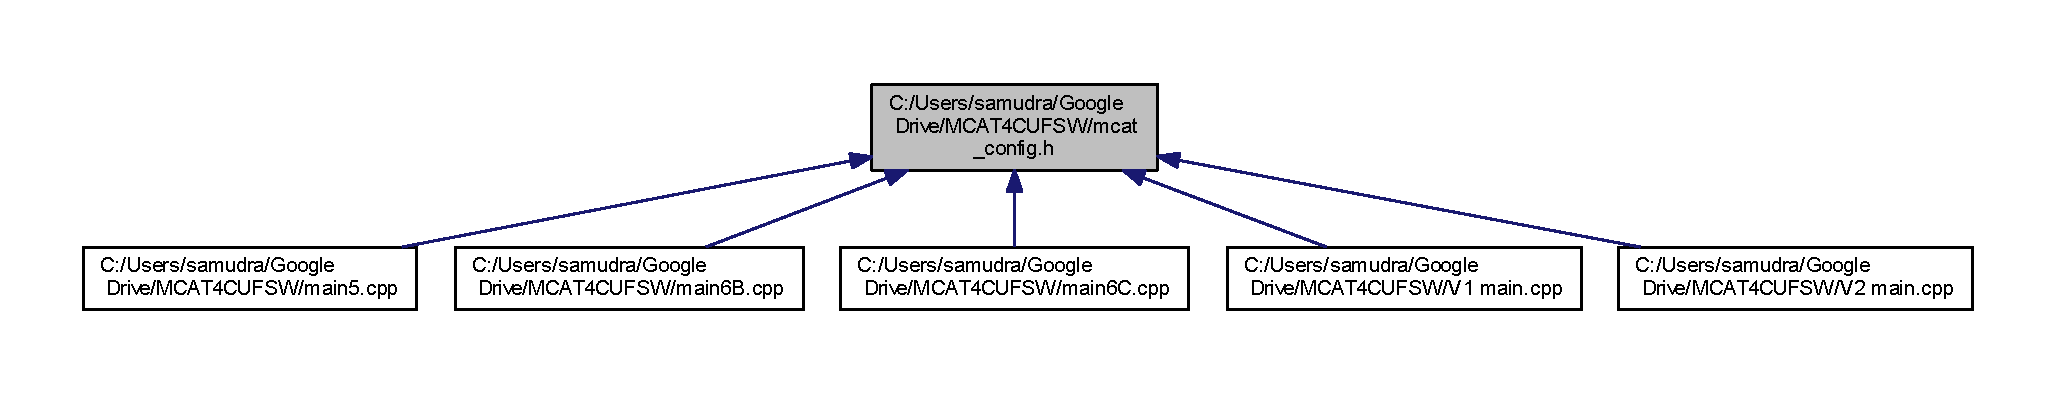
\includegraphics[width=350pt]{mcat__config_8h__dep__incl}
\end{center}
\end{figure}
\subsection*{Macros}
\begin{DoxyCompactItemize}
\item 
\#define \hyperlink{mcat__config_8h_a792042c43305f039f5dc463b0fb00a8a}{G\+R\+O\+U\+N\+D\+T\+E\+S\+T\+I\+N\+G}
\item 
\#define \hyperlink{mcat__config_8h_ad49b84e1d95d80639f908b69662909a5}{M\+C\+A\+T\+\_\+\+P\+P\+U\+\_\+\+C\+H\+A\+N\+N\+E\+L\+S}~4
\item 
\#define \hyperlink{mcat__config_8h_a51ca3f32e04fd99e321851e7dc4109bb}{T\+E\+S\+T\+\_\+\+P\+U\+L\+S\+E\+\_\+\+C\+O\+U\+N\+T}~5
\item 
\#define \hyperlink{mcat__config_8h_a8fe248bd745b90e2bfe94d8c5fce0a53}{C\+U\+\_\+\+I2\+C\+\_\+\+S\+L\+A\+V\+E\+\_\+\+A\+D\+D\+R}~0x26
\item 
\#define \hyperlink{mcat__config_8h_a65b537eaba53f6a2e9baa86e843aa393}{T\+E\+S\+T\+B\+U\+S\+\_\+\+I2\+C\+\_\+\+S\+L\+A\+V\+E\+\_\+\+A\+D\+D\+R}~0x24
\item 
\#define \hyperlink{mcat__config_8h_a178606edb745418f722bc5b76ca83b7f}{C\+U\+\_\+\+S\+U\+B\+S\+Y\+S\+T\+E\+M}~\char`\"{}M\+C\+A\+T-\/4\+C\+U-\/\+B Subsystem\char`\"{}
\item 
\#define \hyperlink{mcat__config_8h_a2a10de88e1c279117a849f8e99647cf4}{C\+U\+\_\+\+P\+R\+O\+J\+E\+C\+T}~\char`\"{}Micro-\/Cathode Arc Thruster Subsystem for U\+S\+N\+A \hyperlink{mcat__config_8h_a8b5032d5e1294a4c6cbc07ff228bc69b}{B\+R\+I\+C\+S\+A\+T}-\/p Cubesat\char`\"{}
\item 
\#define \hyperlink{mcat__config_8h_a08afb324a702457901cbe379650ca9a6}{C\+U\+\_\+\+B\+U\+I\+L\+D\+\_\+\+M\+A\+J\+O\+R}~\char`\"{}6\char`\"{}
\item 
\#define \hyperlink{mcat__config_8h_a298de3c4c7515af07bb38f57ff308fb6}{C\+U\+\_\+\+B\+U\+I\+L\+D\+\_\+\+M\+I\+N\+O\+R}~\char`\"{}C\char`\"{}
\item 
\#define \hyperlink{mcat__config_8h_a6e4e06c6a6b94d8b852e32c6256eca12}{C\+U\+\_\+\+A\+U\+T\+H\+O\+R}~\char`\"{} samudra@gwu.\+edu N3\+R\+D\+X\char`\"{}
\item 
\#define \hyperlink{mcat__config_8h_a8b5032d5e1294a4c6cbc07ff228bc69b}{B\+R\+I\+C\+S\+A\+T}
\item 
\#define \hyperlink{mcat__config_8h_a10a6dc2f7ece97aaee2549972ab74623}{H\+I\+D\+D\+E\+N\+M\+E\+N\+U}
\item 
\#define \hyperlink{mcat__config_8h_a95dacadc0296859d631e0a4da515018e}{C\+U\+\_\+\+V\+E\+R\+S\+I\+O\+N\+\_\+\+L\+E\+N}~10
\item 
\#define \hyperlink{mcat__config_8h_ae841604dc53df3a0b2b2405394b49007}{T\+B\+\_\+\+B\+U\+I\+L\+D\+\_\+\+M\+A\+J\+O\+R}~\char`\"{}1\char`\"{}
\item 
\#define \hyperlink{mcat__config_8h_ab7f921e09fd074ec590533fec2fc18b7}{T\+B\+\_\+\+B\+U\+I\+L\+D\+\_\+\+M\+I\+N\+O\+R}~\char`\"{}A\char`\"{}
\item 
\#define \hyperlink{mcat__config_8h_a754a543ef481b4e8e5da6d65412635fa}{T\+B\+\_\+\+V\+E\+R\+S\+I\+O\+N\+\_\+\+L\+E\+N}~10
\item 
\#define \hyperlink{mcat__config_8h_a50e40f98b0a2e1338e46f50d178434c1}{B\+U\+I\+L\+D\+\_\+\+T\+I\+M\+E\+S\+T\+A\+M\+P}~\char`\"{}201409251844\char`\"{}
\item 
\#define \hyperlink{mcat__config_8h_aa83c1f4aafa1a8610d231d8e2721d4e0}{B\+U\+I\+L\+D\+\_\+\+A\+P\+P\+\_\+\+T\+A\+S\+K\+M\+O\+N}~\char`\"{}M2\+C\+U-\/4\+G\char`\"{}
\item 
\#define \hyperlink{mcat__config_8h_af20537a0b4c7ffdf9df866736be554ab}{B\+U\+I\+L\+D\+\_\+\+A\+P\+P\+\_\+\+T\+I\+T\+L\+E}~\char`\"{}Micro-\/Cathode Arc Thruster 2-\/Ch Control Unit -\/ Remote Test Program\char`\"{}
\item 
\#define \hyperlink{mcat__config_8h_a7f43b36cfbbd59cd83b3193004616f7e}{B\+U\+I\+L\+D\+\_\+\+D\+A\+T\+E}~\+\_\+\+\_\+\+D\+A\+T\+E\+\_\+\+\_\+
\item 
\#define \hyperlink{mcat__config_8h_aa0566a4cbfe1e0d65d5bd7c7eb51b208}{B\+U\+I\+L\+D\+\_\+\+T\+I\+M\+E}~\+\_\+\+\_\+\+T\+I\+M\+E\+\_\+\+\_\+
\end{DoxyCompactItemize}
\subsection*{Variables}
\begin{DoxyCompactItemize}
\item 
char \hyperlink{mcat__config_8h_a872109f1fcc5769fa2b6d36a2f5e2b81}{string\+Version} \mbox{[}2\mbox{]}
\item 
D\+W\+O\+R\+D \hyperlink{mcat__config_8h_aeb542f621e9e8c74bcdc3697fa1103a1}{do\+Pulse\+Stack} \mbox{[}U\+S\+E\+R\+\_\+\+T\+A\+S\+K\+\_\+\+S\+T\+K\+\_\+\+S\+I\+Z\+E\mbox{]}
\item 
D\+W\+O\+R\+D \hyperlink{mcat__config_8h_a3f299d30e105eaf7b8e1ef9dcc0fc969}{uint32\+\_\+counter} = 0
\item 
D\+W\+O\+R\+D \hyperlink{mcat__config_8h_afd595e9237070d595e2ef2557e033180}{Pulse\+Count} = 0
\item 
D\+W\+O\+R\+D \hyperlink{mcat__config_8h_aa32ea573b06e186cfe5ff9072bbeddce}{Max\+Count} = 1
\item 
D\+W\+O\+R\+D \hyperlink{mcat__config_8h_a915c2c2741e3aa74b0a72ff91541faae}{end\+Count\+Ch1} = 0
\item 
D\+W\+O\+R\+D \hyperlink{mcat__config_8h_aba47196705022644eefd0847852bba49}{end\+Count\+Ch2} = 0
\item 
D\+W\+O\+R\+D \hyperlink{mcat__config_8h_a820f0229a4daf8fd96ea0c6fefaa1cdb}{end\+Count\+Ch3} = 0
\item 
D\+W\+O\+R\+D \hyperlink{mcat__config_8h_a8092145363e991dbbad5ed2245e5d394}{end\+Count\+Ch4} = 0
\item 
int \hyperlink{mcat__config_8h_a48f874fc5afc8dc874f26122d06a5e3c}{T\+S1\+Count} = 0
\item 
bool \hyperlink{mcat__config_8h_afe69cf88e006860f320aa426205fbcb5}{Continuous} = F\+A\+L\+S\+E
\item 
O\+S\+\_\+\+S\+E\+M \hyperlink{mcat__config_8h_ac7034a61a410e55fede247ba04e3ff78}{Sem\+Pulse}
\item 
O\+S\+\_\+\+S\+E\+M \hyperlink{mcat__config_8h_a29a48a96d1ce18a4db8cc86c71ed561d}{Semp\+T\+P}
\item 
O\+S\+\_\+\+S\+E\+M \hyperlink{mcat__config_8h_a43e10631e1aa1db599c589aec8f102c8}{P18\+H1\+Sem}
\item 
O\+S\+\_\+\+S\+E\+M \hyperlink{mcat__config_8h_a0648b72849da10cd6903b357965670a6}{P18\+H2\+Sem}
\item 
O\+S\+\_\+\+S\+E\+M \hyperlink{mcat__config_8h_a87fe0657b6d234557abf15548efecbc6}{P18\+H3\+Sem}
\item 
O\+S\+\_\+\+S\+E\+M \hyperlink{mcat__config_8h_a70654fb5aef702a8290428d8e2033798}{P18\+H4\+Sem}
\item 
int \hyperlink{mcat__config_8h_a53d4da6eafff271fd1200dc269a32215}{Ch1\+Prio} =62
\item 
int \hyperlink{mcat__config_8h_a2cdc8e79cd056bff785480a12ec2e195}{Ch2\+Prio} =61
\item 
int \hyperlink{mcat__config_8h_ac99f66a8313974759c4c4c440bdbe099}{Ch3\+Prio} =60
\item 
int \hyperlink{mcat__config_8h_a77e8496684805e4a9f98bb5bc6655266}{Ch4\+Prio} =59
\item 
int \hyperlink{mcat__config_8h_a06f4596b463eb3c49c5fbaf8d53c6b86}{H\+I\+G\+H} =1
\item 
int \hyperlink{mcat__config_8h_a9aaed5df34bfbfa5a77bda384af2da53}{N\+H\+I\+G\+H} = 0
\item 
int \hyperlink{mcat__config_8h_aad1ca03c7ec97a9390cbcb91d85183e2}{L\+O\+W} =0
\item 
int \hyperlink{mcat__config_8h_a0eacf618b269ec65d21e925ec24d683d}{N\+L\+O\+W} = 1
\item 
int \hyperlink{mcat__config_8h_a9a6aafc815ee71040e6704d39ecef31f}{O\+N} =1
\item 
int \hyperlink{mcat__config_8h_ab348a4863075edfb0ee2f41d7aeb89cc}{O\+F\+F} = 0
\item 
int \hyperlink{mcat__config_8h_a024d8e051cc125dce22f0830e6b01079}{A\+C\+T\+I\+V\+E} =1
\item 
int \hyperlink{mcat__config_8h_ab3857378b893e5e151960ea34461bdb4}{I\+N\+A\+C\+T\+I\+V\+E} =0
\item 
int \hyperlink{mcat__config_8h_a63207e29c89e24654279e4ae5650e593}{count\+U\+P}
\item 
D\+W\+O\+R\+D \hyperlink{mcat__config_8h_a5e7a2284fd5ff31f75d507571127f524}{limit\+Pulse\+Count} = 50
\end{DoxyCompactItemize}


\subsection{Macro Definition Documentation}
\hypertarget{mcat__config_8h_a8b5032d5e1294a4c6cbc07ff228bc69b}{}\index{mcat\+\_\+config.\+h@{mcat\+\_\+config.\+h}!B\+R\+I\+C\+S\+A\+T@{B\+R\+I\+C\+S\+A\+T}}
\index{B\+R\+I\+C\+S\+A\+T@{B\+R\+I\+C\+S\+A\+T}!mcat\+\_\+config.\+h@{mcat\+\_\+config.\+h}}
\subsubsection[{B\+R\+I\+C\+S\+A\+T}]{\setlength{\rightskip}{0pt plus 5cm}\#define B\+R\+I\+C\+S\+A\+T}\label{mcat__config_8h_a8b5032d5e1294a4c6cbc07ff228bc69b}


Definition at line 103 of file mcat\+\_\+config.\+h.

\hypertarget{mcat__config_8h_aa83c1f4aafa1a8610d231d8e2721d4e0}{}\index{mcat\+\_\+config.\+h@{mcat\+\_\+config.\+h}!B\+U\+I\+L\+D\+\_\+\+A\+P\+P\+\_\+\+T\+A\+S\+K\+M\+O\+N@{B\+U\+I\+L\+D\+\_\+\+A\+P\+P\+\_\+\+T\+A\+S\+K\+M\+O\+N}}
\index{B\+U\+I\+L\+D\+\_\+\+A\+P\+P\+\_\+\+T\+A\+S\+K\+M\+O\+N@{B\+U\+I\+L\+D\+\_\+\+A\+P\+P\+\_\+\+T\+A\+S\+K\+M\+O\+N}!mcat\+\_\+config.\+h@{mcat\+\_\+config.\+h}}
\subsubsection[{B\+U\+I\+L\+D\+\_\+\+A\+P\+P\+\_\+\+T\+A\+S\+K\+M\+O\+N}]{\setlength{\rightskip}{0pt plus 5cm}\#define B\+U\+I\+L\+D\+\_\+\+A\+P\+P\+\_\+\+T\+A\+S\+K\+M\+O\+N~\char`\"{}M2\+C\+U-\/4\+G\char`\"{}}\label{mcat__config_8h_aa83c1f4aafa1a8610d231d8e2721d4e0}


Definition at line 134 of file mcat\+\_\+config.\+h.

\hypertarget{mcat__config_8h_af20537a0b4c7ffdf9df866736be554ab}{}\index{mcat\+\_\+config.\+h@{mcat\+\_\+config.\+h}!B\+U\+I\+L\+D\+\_\+\+A\+P\+P\+\_\+\+T\+I\+T\+L\+E@{B\+U\+I\+L\+D\+\_\+\+A\+P\+P\+\_\+\+T\+I\+T\+L\+E}}
\index{B\+U\+I\+L\+D\+\_\+\+A\+P\+P\+\_\+\+T\+I\+T\+L\+E@{B\+U\+I\+L\+D\+\_\+\+A\+P\+P\+\_\+\+T\+I\+T\+L\+E}!mcat\+\_\+config.\+h@{mcat\+\_\+config.\+h}}
\subsubsection[{B\+U\+I\+L\+D\+\_\+\+A\+P\+P\+\_\+\+T\+I\+T\+L\+E}]{\setlength{\rightskip}{0pt plus 5cm}\#define B\+U\+I\+L\+D\+\_\+\+A\+P\+P\+\_\+\+T\+I\+T\+L\+E~\char`\"{}Micro-\/Cathode Arc Thruster 2-\/Ch Control Unit -\/ Remote Test Program\char`\"{}}\label{mcat__config_8h_af20537a0b4c7ffdf9df866736be554ab}


Definition at line 135 of file mcat\+\_\+config.\+h.

\hypertarget{mcat__config_8h_a7f43b36cfbbd59cd83b3193004616f7e}{}\index{mcat\+\_\+config.\+h@{mcat\+\_\+config.\+h}!B\+U\+I\+L\+D\+\_\+\+D\+A\+T\+E@{B\+U\+I\+L\+D\+\_\+\+D\+A\+T\+E}}
\index{B\+U\+I\+L\+D\+\_\+\+D\+A\+T\+E@{B\+U\+I\+L\+D\+\_\+\+D\+A\+T\+E}!mcat\+\_\+config.\+h@{mcat\+\_\+config.\+h}}
\subsubsection[{B\+U\+I\+L\+D\+\_\+\+D\+A\+T\+E}]{\setlength{\rightskip}{0pt plus 5cm}\#define B\+U\+I\+L\+D\+\_\+\+D\+A\+T\+E~\+\_\+\+\_\+\+D\+A\+T\+E\+\_\+\+\_\+}\label{mcat__config_8h_a7f43b36cfbbd59cd83b3193004616f7e}


Definition at line 136 of file mcat\+\_\+config.\+h.

\hypertarget{mcat__config_8h_aa0566a4cbfe1e0d65d5bd7c7eb51b208}{}\index{mcat\+\_\+config.\+h@{mcat\+\_\+config.\+h}!B\+U\+I\+L\+D\+\_\+\+T\+I\+M\+E@{B\+U\+I\+L\+D\+\_\+\+T\+I\+M\+E}}
\index{B\+U\+I\+L\+D\+\_\+\+T\+I\+M\+E@{B\+U\+I\+L\+D\+\_\+\+T\+I\+M\+E}!mcat\+\_\+config.\+h@{mcat\+\_\+config.\+h}}
\subsubsection[{B\+U\+I\+L\+D\+\_\+\+T\+I\+M\+E}]{\setlength{\rightskip}{0pt plus 5cm}\#define B\+U\+I\+L\+D\+\_\+\+T\+I\+M\+E~\+\_\+\+\_\+\+T\+I\+M\+E\+\_\+\+\_\+}\label{mcat__config_8h_aa0566a4cbfe1e0d65d5bd7c7eb51b208}


Definition at line 137 of file mcat\+\_\+config.\+h.

\hypertarget{mcat__config_8h_a50e40f98b0a2e1338e46f50d178434c1}{}\index{mcat\+\_\+config.\+h@{mcat\+\_\+config.\+h}!B\+U\+I\+L\+D\+\_\+\+T\+I\+M\+E\+S\+T\+A\+M\+P@{B\+U\+I\+L\+D\+\_\+\+T\+I\+M\+E\+S\+T\+A\+M\+P}}
\index{B\+U\+I\+L\+D\+\_\+\+T\+I\+M\+E\+S\+T\+A\+M\+P@{B\+U\+I\+L\+D\+\_\+\+T\+I\+M\+E\+S\+T\+A\+M\+P}!mcat\+\_\+config.\+h@{mcat\+\_\+config.\+h}}
\subsubsection[{B\+U\+I\+L\+D\+\_\+\+T\+I\+M\+E\+S\+T\+A\+M\+P}]{\setlength{\rightskip}{0pt plus 5cm}\#define B\+U\+I\+L\+D\+\_\+\+T\+I\+M\+E\+S\+T\+A\+M\+P~\char`\"{}201409251844\char`\"{}}\label{mcat__config_8h_a50e40f98b0a2e1338e46f50d178434c1}


Definition at line 133 of file mcat\+\_\+config.\+h.

\hypertarget{mcat__config_8h_a6e4e06c6a6b94d8b852e32c6256eca12}{}\index{mcat\+\_\+config.\+h@{mcat\+\_\+config.\+h}!C\+U\+\_\+\+A\+U\+T\+H\+O\+R@{C\+U\+\_\+\+A\+U\+T\+H\+O\+R}}
\index{C\+U\+\_\+\+A\+U\+T\+H\+O\+R@{C\+U\+\_\+\+A\+U\+T\+H\+O\+R}!mcat\+\_\+config.\+h@{mcat\+\_\+config.\+h}}
\subsubsection[{C\+U\+\_\+\+A\+U\+T\+H\+O\+R}]{\setlength{\rightskip}{0pt plus 5cm}\#define C\+U\+\_\+\+A\+U\+T\+H\+O\+R~\char`\"{} samudra@gwu.\+edu N3\+R\+D\+X\char`\"{}}\label{mcat__config_8h_a6e4e06c6a6b94d8b852e32c6256eca12}


Definition at line 99 of file mcat\+\_\+config.\+h.

\hypertarget{mcat__config_8h_a08afb324a702457901cbe379650ca9a6}{}\index{mcat\+\_\+config.\+h@{mcat\+\_\+config.\+h}!C\+U\+\_\+\+B\+U\+I\+L\+D\+\_\+\+M\+A\+J\+O\+R@{C\+U\+\_\+\+B\+U\+I\+L\+D\+\_\+\+M\+A\+J\+O\+R}}
\index{C\+U\+\_\+\+B\+U\+I\+L\+D\+\_\+\+M\+A\+J\+O\+R@{C\+U\+\_\+\+B\+U\+I\+L\+D\+\_\+\+M\+A\+J\+O\+R}!mcat\+\_\+config.\+h@{mcat\+\_\+config.\+h}}
\subsubsection[{C\+U\+\_\+\+B\+U\+I\+L\+D\+\_\+\+M\+A\+J\+O\+R}]{\setlength{\rightskip}{0pt plus 5cm}\#define C\+U\+\_\+\+B\+U\+I\+L\+D\+\_\+\+M\+A\+J\+O\+R~\char`\"{}6\char`\"{}}\label{mcat__config_8h_a08afb324a702457901cbe379650ca9a6}


Definition at line 97 of file mcat\+\_\+config.\+h.

\hypertarget{mcat__config_8h_a298de3c4c7515af07bb38f57ff308fb6}{}\index{mcat\+\_\+config.\+h@{mcat\+\_\+config.\+h}!C\+U\+\_\+\+B\+U\+I\+L\+D\+\_\+\+M\+I\+N\+O\+R@{C\+U\+\_\+\+B\+U\+I\+L\+D\+\_\+\+M\+I\+N\+O\+R}}
\index{C\+U\+\_\+\+B\+U\+I\+L\+D\+\_\+\+M\+I\+N\+O\+R@{C\+U\+\_\+\+B\+U\+I\+L\+D\+\_\+\+M\+I\+N\+O\+R}!mcat\+\_\+config.\+h@{mcat\+\_\+config.\+h}}
\subsubsection[{C\+U\+\_\+\+B\+U\+I\+L\+D\+\_\+\+M\+I\+N\+O\+R}]{\setlength{\rightskip}{0pt plus 5cm}\#define C\+U\+\_\+\+B\+U\+I\+L\+D\+\_\+\+M\+I\+N\+O\+R~\char`\"{}C\char`\"{}}\label{mcat__config_8h_a298de3c4c7515af07bb38f57ff308fb6}


Definition at line 98 of file mcat\+\_\+config.\+h.

\hypertarget{mcat__config_8h_a8fe248bd745b90e2bfe94d8c5fce0a53}{}\index{mcat\+\_\+config.\+h@{mcat\+\_\+config.\+h}!C\+U\+\_\+\+I2\+C\+\_\+\+S\+L\+A\+V\+E\+\_\+\+A\+D\+D\+R@{C\+U\+\_\+\+I2\+C\+\_\+\+S\+L\+A\+V\+E\+\_\+\+A\+D\+D\+R}}
\index{C\+U\+\_\+\+I2\+C\+\_\+\+S\+L\+A\+V\+E\+\_\+\+A\+D\+D\+R@{C\+U\+\_\+\+I2\+C\+\_\+\+S\+L\+A\+V\+E\+\_\+\+A\+D\+D\+R}!mcat\+\_\+config.\+h@{mcat\+\_\+config.\+h}}
\subsubsection[{C\+U\+\_\+\+I2\+C\+\_\+\+S\+L\+A\+V\+E\+\_\+\+A\+D\+D\+R}]{\setlength{\rightskip}{0pt plus 5cm}\#define C\+U\+\_\+\+I2\+C\+\_\+\+S\+L\+A\+V\+E\+\_\+\+A\+D\+D\+R~0x26}\label{mcat__config_8h_a8fe248bd745b90e2bfe94d8c5fce0a53}


Definition at line 89 of file mcat\+\_\+config.\+h.

\hypertarget{mcat__config_8h_a2a10de88e1c279117a849f8e99647cf4}{}\index{mcat\+\_\+config.\+h@{mcat\+\_\+config.\+h}!C\+U\+\_\+\+P\+R\+O\+J\+E\+C\+T@{C\+U\+\_\+\+P\+R\+O\+J\+E\+C\+T}}
\index{C\+U\+\_\+\+P\+R\+O\+J\+E\+C\+T@{C\+U\+\_\+\+P\+R\+O\+J\+E\+C\+T}!mcat\+\_\+config.\+h@{mcat\+\_\+config.\+h}}
\subsubsection[{C\+U\+\_\+\+P\+R\+O\+J\+E\+C\+T}]{\setlength{\rightskip}{0pt plus 5cm}\#define C\+U\+\_\+\+P\+R\+O\+J\+E\+C\+T~\char`\"{}Micro-\/Cathode Arc Thruster Subsystem for U\+S\+N\+A {\bf B\+R\+I\+C\+S\+A\+T}-\/p Cubesat\char`\"{}}\label{mcat__config_8h_a2a10de88e1c279117a849f8e99647cf4}


Definition at line 96 of file mcat\+\_\+config.\+h.

\hypertarget{mcat__config_8h_a178606edb745418f722bc5b76ca83b7f}{}\index{mcat\+\_\+config.\+h@{mcat\+\_\+config.\+h}!C\+U\+\_\+\+S\+U\+B\+S\+Y\+S\+T\+E\+M@{C\+U\+\_\+\+S\+U\+B\+S\+Y\+S\+T\+E\+M}}
\index{C\+U\+\_\+\+S\+U\+B\+S\+Y\+S\+T\+E\+M@{C\+U\+\_\+\+S\+U\+B\+S\+Y\+S\+T\+E\+M}!mcat\+\_\+config.\+h@{mcat\+\_\+config.\+h}}
\subsubsection[{C\+U\+\_\+\+S\+U\+B\+S\+Y\+S\+T\+E\+M}]{\setlength{\rightskip}{0pt plus 5cm}\#define C\+U\+\_\+\+S\+U\+B\+S\+Y\+S\+T\+E\+M~\char`\"{}M\+C\+A\+T-\/4\+C\+U-\/\+B Subsystem\char`\"{}}\label{mcat__config_8h_a178606edb745418f722bc5b76ca83b7f}


Definition at line 95 of file mcat\+\_\+config.\+h.

\hypertarget{mcat__config_8h_a95dacadc0296859d631e0a4da515018e}{}\index{mcat\+\_\+config.\+h@{mcat\+\_\+config.\+h}!C\+U\+\_\+\+V\+E\+R\+S\+I\+O\+N\+\_\+\+L\+E\+N@{C\+U\+\_\+\+V\+E\+R\+S\+I\+O\+N\+\_\+\+L\+E\+N}}
\index{C\+U\+\_\+\+V\+E\+R\+S\+I\+O\+N\+\_\+\+L\+E\+N@{C\+U\+\_\+\+V\+E\+R\+S\+I\+O\+N\+\_\+\+L\+E\+N}!mcat\+\_\+config.\+h@{mcat\+\_\+config.\+h}}
\subsubsection[{C\+U\+\_\+\+V\+E\+R\+S\+I\+O\+N\+\_\+\+L\+E\+N}]{\setlength{\rightskip}{0pt plus 5cm}\#define C\+U\+\_\+\+V\+E\+R\+S\+I\+O\+N\+\_\+\+L\+E\+N~10}\label{mcat__config_8h_a95dacadc0296859d631e0a4da515018e}


Definition at line 116 of file mcat\+\_\+config.\+h.

\hypertarget{mcat__config_8h_a792042c43305f039f5dc463b0fb00a8a}{}\index{mcat\+\_\+config.\+h@{mcat\+\_\+config.\+h}!G\+R\+O\+U\+N\+D\+T\+E\+S\+T\+I\+N\+G@{G\+R\+O\+U\+N\+D\+T\+E\+S\+T\+I\+N\+G}}
\index{G\+R\+O\+U\+N\+D\+T\+E\+S\+T\+I\+N\+G@{G\+R\+O\+U\+N\+D\+T\+E\+S\+T\+I\+N\+G}!mcat\+\_\+config.\+h@{mcat\+\_\+config.\+h}}
\subsubsection[{G\+R\+O\+U\+N\+D\+T\+E\+S\+T\+I\+N\+G}]{\setlength{\rightskip}{0pt plus 5cm}\#define G\+R\+O\+U\+N\+D\+T\+E\+S\+T\+I\+N\+G}\label{mcat__config_8h_a792042c43305f039f5dc463b0fb00a8a}


Definition at line 14 of file mcat\+\_\+config.\+h.

\hypertarget{mcat__config_8h_a10a6dc2f7ece97aaee2549972ab74623}{}\index{mcat\+\_\+config.\+h@{mcat\+\_\+config.\+h}!H\+I\+D\+D\+E\+N\+M\+E\+N\+U@{H\+I\+D\+D\+E\+N\+M\+E\+N\+U}}
\index{H\+I\+D\+D\+E\+N\+M\+E\+N\+U@{H\+I\+D\+D\+E\+N\+M\+E\+N\+U}!mcat\+\_\+config.\+h@{mcat\+\_\+config.\+h}}
\subsubsection[{H\+I\+D\+D\+E\+N\+M\+E\+N\+U}]{\setlength{\rightskip}{0pt plus 5cm}\#define H\+I\+D\+D\+E\+N\+M\+E\+N\+U}\label{mcat__config_8h_a10a6dc2f7ece97aaee2549972ab74623}


Definition at line 104 of file mcat\+\_\+config.\+h.

\hypertarget{mcat__config_8h_ad49b84e1d95d80639f908b69662909a5}{}\index{mcat\+\_\+config.\+h@{mcat\+\_\+config.\+h}!M\+C\+A\+T\+\_\+\+P\+P\+U\+\_\+\+C\+H\+A\+N\+N\+E\+L\+S@{M\+C\+A\+T\+\_\+\+P\+P\+U\+\_\+\+C\+H\+A\+N\+N\+E\+L\+S}}
\index{M\+C\+A\+T\+\_\+\+P\+P\+U\+\_\+\+C\+H\+A\+N\+N\+E\+L\+S@{M\+C\+A\+T\+\_\+\+P\+P\+U\+\_\+\+C\+H\+A\+N\+N\+E\+L\+S}!mcat\+\_\+config.\+h@{mcat\+\_\+config.\+h}}
\subsubsection[{M\+C\+A\+T\+\_\+\+P\+P\+U\+\_\+\+C\+H\+A\+N\+N\+E\+L\+S}]{\setlength{\rightskip}{0pt plus 5cm}\#define M\+C\+A\+T\+\_\+\+P\+P\+U\+\_\+\+C\+H\+A\+N\+N\+E\+L\+S~4}\label{mcat__config_8h_ad49b84e1d95d80639f908b69662909a5}


Definition at line 50 of file mcat\+\_\+config.\+h.

\hypertarget{mcat__config_8h_ae841604dc53df3a0b2b2405394b49007}{}\index{mcat\+\_\+config.\+h@{mcat\+\_\+config.\+h}!T\+B\+\_\+\+B\+U\+I\+L\+D\+\_\+\+M\+A\+J\+O\+R@{T\+B\+\_\+\+B\+U\+I\+L\+D\+\_\+\+M\+A\+J\+O\+R}}
\index{T\+B\+\_\+\+B\+U\+I\+L\+D\+\_\+\+M\+A\+J\+O\+R@{T\+B\+\_\+\+B\+U\+I\+L\+D\+\_\+\+M\+A\+J\+O\+R}!mcat\+\_\+config.\+h@{mcat\+\_\+config.\+h}}
\subsubsection[{T\+B\+\_\+\+B\+U\+I\+L\+D\+\_\+\+M\+A\+J\+O\+R}]{\setlength{\rightskip}{0pt plus 5cm}\#define T\+B\+\_\+\+B\+U\+I\+L\+D\+\_\+\+M\+A\+J\+O\+R~\char`\"{}1\char`\"{}}\label{mcat__config_8h_ae841604dc53df3a0b2b2405394b49007}


Definition at line 126 of file mcat\+\_\+config.\+h.

\hypertarget{mcat__config_8h_ab7f921e09fd074ec590533fec2fc18b7}{}\index{mcat\+\_\+config.\+h@{mcat\+\_\+config.\+h}!T\+B\+\_\+\+B\+U\+I\+L\+D\+\_\+\+M\+I\+N\+O\+R@{T\+B\+\_\+\+B\+U\+I\+L\+D\+\_\+\+M\+I\+N\+O\+R}}
\index{T\+B\+\_\+\+B\+U\+I\+L\+D\+\_\+\+M\+I\+N\+O\+R@{T\+B\+\_\+\+B\+U\+I\+L\+D\+\_\+\+M\+I\+N\+O\+R}!mcat\+\_\+config.\+h@{mcat\+\_\+config.\+h}}
\subsubsection[{T\+B\+\_\+\+B\+U\+I\+L\+D\+\_\+\+M\+I\+N\+O\+R}]{\setlength{\rightskip}{0pt plus 5cm}\#define T\+B\+\_\+\+B\+U\+I\+L\+D\+\_\+\+M\+I\+N\+O\+R~\char`\"{}A\char`\"{}}\label{mcat__config_8h_ab7f921e09fd074ec590533fec2fc18b7}


Definition at line 127 of file mcat\+\_\+config.\+h.

\hypertarget{mcat__config_8h_a754a543ef481b4e8e5da6d65412635fa}{}\index{mcat\+\_\+config.\+h@{mcat\+\_\+config.\+h}!T\+B\+\_\+\+V\+E\+R\+S\+I\+O\+N\+\_\+\+L\+E\+N@{T\+B\+\_\+\+V\+E\+R\+S\+I\+O\+N\+\_\+\+L\+E\+N}}
\index{T\+B\+\_\+\+V\+E\+R\+S\+I\+O\+N\+\_\+\+L\+E\+N@{T\+B\+\_\+\+V\+E\+R\+S\+I\+O\+N\+\_\+\+L\+E\+N}!mcat\+\_\+config.\+h@{mcat\+\_\+config.\+h}}
\subsubsection[{T\+B\+\_\+\+V\+E\+R\+S\+I\+O\+N\+\_\+\+L\+E\+N}]{\setlength{\rightskip}{0pt plus 5cm}\#define T\+B\+\_\+\+V\+E\+R\+S\+I\+O\+N\+\_\+\+L\+E\+N~10}\label{mcat__config_8h_a754a543ef481b4e8e5da6d65412635fa}


Definition at line 128 of file mcat\+\_\+config.\+h.

\hypertarget{mcat__config_8h_a51ca3f32e04fd99e321851e7dc4109bb}{}\index{mcat\+\_\+config.\+h@{mcat\+\_\+config.\+h}!T\+E\+S\+T\+\_\+\+P\+U\+L\+S\+E\+\_\+\+C\+O\+U\+N\+T@{T\+E\+S\+T\+\_\+\+P\+U\+L\+S\+E\+\_\+\+C\+O\+U\+N\+T}}
\index{T\+E\+S\+T\+\_\+\+P\+U\+L\+S\+E\+\_\+\+C\+O\+U\+N\+T@{T\+E\+S\+T\+\_\+\+P\+U\+L\+S\+E\+\_\+\+C\+O\+U\+N\+T}!mcat\+\_\+config.\+h@{mcat\+\_\+config.\+h}}
\subsubsection[{T\+E\+S\+T\+\_\+\+P\+U\+L\+S\+E\+\_\+\+C\+O\+U\+N\+T}]{\setlength{\rightskip}{0pt plus 5cm}\#define T\+E\+S\+T\+\_\+\+P\+U\+L\+S\+E\+\_\+\+C\+O\+U\+N\+T~5}\label{mcat__config_8h_a51ca3f32e04fd99e321851e7dc4109bb}


Definition at line 51 of file mcat\+\_\+config.\+h.

\hypertarget{mcat__config_8h_a65b537eaba53f6a2e9baa86e843aa393}{}\index{mcat\+\_\+config.\+h@{mcat\+\_\+config.\+h}!T\+E\+S\+T\+B\+U\+S\+\_\+\+I2\+C\+\_\+\+S\+L\+A\+V\+E\+\_\+\+A\+D\+D\+R@{T\+E\+S\+T\+B\+U\+S\+\_\+\+I2\+C\+\_\+\+S\+L\+A\+V\+E\+\_\+\+A\+D\+D\+R}}
\index{T\+E\+S\+T\+B\+U\+S\+\_\+\+I2\+C\+\_\+\+S\+L\+A\+V\+E\+\_\+\+A\+D\+D\+R@{T\+E\+S\+T\+B\+U\+S\+\_\+\+I2\+C\+\_\+\+S\+L\+A\+V\+E\+\_\+\+A\+D\+D\+R}!mcat\+\_\+config.\+h@{mcat\+\_\+config.\+h}}
\subsubsection[{T\+E\+S\+T\+B\+U\+S\+\_\+\+I2\+C\+\_\+\+S\+L\+A\+V\+E\+\_\+\+A\+D\+D\+R}]{\setlength{\rightskip}{0pt plus 5cm}\#define T\+E\+S\+T\+B\+U\+S\+\_\+\+I2\+C\+\_\+\+S\+L\+A\+V\+E\+\_\+\+A\+D\+D\+R~0x24}\label{mcat__config_8h_a65b537eaba53f6a2e9baa86e843aa393}


Definition at line 90 of file mcat\+\_\+config.\+h.



\subsection{Variable Documentation}
\hypertarget{mcat__config_8h_a024d8e051cc125dce22f0830e6b01079}{}\index{mcat\+\_\+config.\+h@{mcat\+\_\+config.\+h}!A\+C\+T\+I\+V\+E@{A\+C\+T\+I\+V\+E}}
\index{A\+C\+T\+I\+V\+E@{A\+C\+T\+I\+V\+E}!mcat\+\_\+config.\+h@{mcat\+\_\+config.\+h}}
\subsubsection[{A\+C\+T\+I\+V\+E}]{\setlength{\rightskip}{0pt plus 5cm}int A\+C\+T\+I\+V\+E =1}\label{mcat__config_8h_a024d8e051cc125dce22f0830e6b01079}


Definition at line 46 of file mcat\+\_\+config.\+h.

\hypertarget{mcat__config_8h_a53d4da6eafff271fd1200dc269a32215}{}\index{mcat\+\_\+config.\+h@{mcat\+\_\+config.\+h}!Ch1\+Prio@{Ch1\+Prio}}
\index{Ch1\+Prio@{Ch1\+Prio}!mcat\+\_\+config.\+h@{mcat\+\_\+config.\+h}}
\subsubsection[{Ch1\+Prio}]{\setlength{\rightskip}{0pt plus 5cm}int Ch1\+Prio =62}\label{mcat__config_8h_a53d4da6eafff271fd1200dc269a32215}


Definition at line 37 of file mcat\+\_\+config.\+h.

\hypertarget{mcat__config_8h_a2cdc8e79cd056bff785480a12ec2e195}{}\index{mcat\+\_\+config.\+h@{mcat\+\_\+config.\+h}!Ch2\+Prio@{Ch2\+Prio}}
\index{Ch2\+Prio@{Ch2\+Prio}!mcat\+\_\+config.\+h@{mcat\+\_\+config.\+h}}
\subsubsection[{Ch2\+Prio}]{\setlength{\rightskip}{0pt plus 5cm}int Ch2\+Prio =61}\label{mcat__config_8h_a2cdc8e79cd056bff785480a12ec2e195}


Definition at line 38 of file mcat\+\_\+config.\+h.

\hypertarget{mcat__config_8h_ac99f66a8313974759c4c4c440bdbe099}{}\index{mcat\+\_\+config.\+h@{mcat\+\_\+config.\+h}!Ch3\+Prio@{Ch3\+Prio}}
\index{Ch3\+Prio@{Ch3\+Prio}!mcat\+\_\+config.\+h@{mcat\+\_\+config.\+h}}
\subsubsection[{Ch3\+Prio}]{\setlength{\rightskip}{0pt plus 5cm}int Ch3\+Prio =60}\label{mcat__config_8h_ac99f66a8313974759c4c4c440bdbe099}


Definition at line 39 of file mcat\+\_\+config.\+h.

\hypertarget{mcat__config_8h_a77e8496684805e4a9f98bb5bc6655266}{}\index{mcat\+\_\+config.\+h@{mcat\+\_\+config.\+h}!Ch4\+Prio@{Ch4\+Prio}}
\index{Ch4\+Prio@{Ch4\+Prio}!mcat\+\_\+config.\+h@{mcat\+\_\+config.\+h}}
\subsubsection[{Ch4\+Prio}]{\setlength{\rightskip}{0pt plus 5cm}int Ch4\+Prio =59}\label{mcat__config_8h_a77e8496684805e4a9f98bb5bc6655266}


Definition at line 40 of file mcat\+\_\+config.\+h.

\hypertarget{mcat__config_8h_afe69cf88e006860f320aa426205fbcb5}{}\index{mcat\+\_\+config.\+h@{mcat\+\_\+config.\+h}!Continuous@{Continuous}}
\index{Continuous@{Continuous}!mcat\+\_\+config.\+h@{mcat\+\_\+config.\+h}}
\subsubsection[{Continuous}]{\setlength{\rightskip}{0pt plus 5cm}bool Continuous = F\+A\+L\+S\+E}\label{mcat__config_8h_afe69cf88e006860f320aa426205fbcb5}


Definition at line 30 of file mcat\+\_\+config.\+h.

\hypertarget{mcat__config_8h_a63207e29c89e24654279e4ae5650e593}{}\index{mcat\+\_\+config.\+h@{mcat\+\_\+config.\+h}!count\+U\+P@{count\+U\+P}}
\index{count\+U\+P@{count\+U\+P}!mcat\+\_\+config.\+h@{mcat\+\_\+config.\+h}}
\subsubsection[{count\+U\+P}]{\setlength{\rightskip}{0pt plus 5cm}int count\+U\+P}\label{mcat__config_8h_a63207e29c89e24654279e4ae5650e593}


Definition at line 48 of file mcat\+\_\+config.\+h.

\hypertarget{mcat__config_8h_aeb542f621e9e8c74bcdc3697fa1103a1}{}\index{mcat\+\_\+config.\+h@{mcat\+\_\+config.\+h}!do\+Pulse\+Stack@{do\+Pulse\+Stack}}
\index{do\+Pulse\+Stack@{do\+Pulse\+Stack}!mcat\+\_\+config.\+h@{mcat\+\_\+config.\+h}}
\subsubsection[{do\+Pulse\+Stack}]{\setlength{\rightskip}{0pt plus 5cm}D\+W\+O\+R\+D do\+Pulse\+Stack\mbox{[}U\+S\+E\+R\+\_\+\+T\+A\+S\+K\+\_\+\+S\+T\+K\+\_\+\+S\+I\+Z\+E\mbox{]}}\label{mcat__config_8h_aeb542f621e9e8c74bcdc3697fa1103a1}


Definition at line 21 of file mcat\+\_\+config.\+h.

\hypertarget{mcat__config_8h_a915c2c2741e3aa74b0a72ff91541faae}{}\index{mcat\+\_\+config.\+h@{mcat\+\_\+config.\+h}!end\+Count\+Ch1@{end\+Count\+Ch1}}
\index{end\+Count\+Ch1@{end\+Count\+Ch1}!mcat\+\_\+config.\+h@{mcat\+\_\+config.\+h}}
\subsubsection[{end\+Count\+Ch1}]{\setlength{\rightskip}{0pt plus 5cm}D\+W\+O\+R\+D end\+Count\+Ch1 = 0}\label{mcat__config_8h_a915c2c2741e3aa74b0a72ff91541faae}


Definition at line 25 of file mcat\+\_\+config.\+h.

\hypertarget{mcat__config_8h_aba47196705022644eefd0847852bba49}{}\index{mcat\+\_\+config.\+h@{mcat\+\_\+config.\+h}!end\+Count\+Ch2@{end\+Count\+Ch2}}
\index{end\+Count\+Ch2@{end\+Count\+Ch2}!mcat\+\_\+config.\+h@{mcat\+\_\+config.\+h}}
\subsubsection[{end\+Count\+Ch2}]{\setlength{\rightskip}{0pt plus 5cm}D\+W\+O\+R\+D end\+Count\+Ch2 = 0}\label{mcat__config_8h_aba47196705022644eefd0847852bba49}


Definition at line 26 of file mcat\+\_\+config.\+h.

\hypertarget{mcat__config_8h_a820f0229a4daf8fd96ea0c6fefaa1cdb}{}\index{mcat\+\_\+config.\+h@{mcat\+\_\+config.\+h}!end\+Count\+Ch3@{end\+Count\+Ch3}}
\index{end\+Count\+Ch3@{end\+Count\+Ch3}!mcat\+\_\+config.\+h@{mcat\+\_\+config.\+h}}
\subsubsection[{end\+Count\+Ch3}]{\setlength{\rightskip}{0pt plus 5cm}D\+W\+O\+R\+D end\+Count\+Ch3 = 0}\label{mcat__config_8h_a820f0229a4daf8fd96ea0c6fefaa1cdb}


Definition at line 27 of file mcat\+\_\+config.\+h.

\hypertarget{mcat__config_8h_a8092145363e991dbbad5ed2245e5d394}{}\index{mcat\+\_\+config.\+h@{mcat\+\_\+config.\+h}!end\+Count\+Ch4@{end\+Count\+Ch4}}
\index{end\+Count\+Ch4@{end\+Count\+Ch4}!mcat\+\_\+config.\+h@{mcat\+\_\+config.\+h}}
\subsubsection[{end\+Count\+Ch4}]{\setlength{\rightskip}{0pt plus 5cm}D\+W\+O\+R\+D end\+Count\+Ch4 = 0}\label{mcat__config_8h_a8092145363e991dbbad5ed2245e5d394}


Definition at line 28 of file mcat\+\_\+config.\+h.

\hypertarget{mcat__config_8h_a06f4596b463eb3c49c5fbaf8d53c6b86}{}\index{mcat\+\_\+config.\+h@{mcat\+\_\+config.\+h}!H\+I\+G\+H@{H\+I\+G\+H}}
\index{H\+I\+G\+H@{H\+I\+G\+H}!mcat\+\_\+config.\+h@{mcat\+\_\+config.\+h}}
\subsubsection[{H\+I\+G\+H}]{\setlength{\rightskip}{0pt plus 5cm}int H\+I\+G\+H =1}\label{mcat__config_8h_a06f4596b463eb3c49c5fbaf8d53c6b86}


Definition at line 43 of file mcat\+\_\+config.\+h.

\hypertarget{mcat__config_8h_ab3857378b893e5e151960ea34461bdb4}{}\index{mcat\+\_\+config.\+h@{mcat\+\_\+config.\+h}!I\+N\+A\+C\+T\+I\+V\+E@{I\+N\+A\+C\+T\+I\+V\+E}}
\index{I\+N\+A\+C\+T\+I\+V\+E@{I\+N\+A\+C\+T\+I\+V\+E}!mcat\+\_\+config.\+h@{mcat\+\_\+config.\+h}}
\subsubsection[{I\+N\+A\+C\+T\+I\+V\+E}]{\setlength{\rightskip}{0pt plus 5cm}int I\+N\+A\+C\+T\+I\+V\+E =0}\label{mcat__config_8h_ab3857378b893e5e151960ea34461bdb4}


Definition at line 46 of file mcat\+\_\+config.\+h.

\hypertarget{mcat__config_8h_a5e7a2284fd5ff31f75d507571127f524}{}\index{mcat\+\_\+config.\+h@{mcat\+\_\+config.\+h}!limit\+Pulse\+Count@{limit\+Pulse\+Count}}
\index{limit\+Pulse\+Count@{limit\+Pulse\+Count}!mcat\+\_\+config.\+h@{mcat\+\_\+config.\+h}}
\subsubsection[{limit\+Pulse\+Count}]{\setlength{\rightskip}{0pt plus 5cm}D\+W\+O\+R\+D limit\+Pulse\+Count = 50}\label{mcat__config_8h_a5e7a2284fd5ff31f75d507571127f524}


Definition at line 107 of file mcat\+\_\+config.\+h.

\hypertarget{mcat__config_8h_aad1ca03c7ec97a9390cbcb91d85183e2}{}\index{mcat\+\_\+config.\+h@{mcat\+\_\+config.\+h}!L\+O\+W@{L\+O\+W}}
\index{L\+O\+W@{L\+O\+W}!mcat\+\_\+config.\+h@{mcat\+\_\+config.\+h}}
\subsubsection[{L\+O\+W}]{\setlength{\rightskip}{0pt plus 5cm}int L\+O\+W =0}\label{mcat__config_8h_aad1ca03c7ec97a9390cbcb91d85183e2}


Definition at line 44 of file mcat\+\_\+config.\+h.

\hypertarget{mcat__config_8h_aa32ea573b06e186cfe5ff9072bbeddce}{}\index{mcat\+\_\+config.\+h@{mcat\+\_\+config.\+h}!Max\+Count@{Max\+Count}}
\index{Max\+Count@{Max\+Count}!mcat\+\_\+config.\+h@{mcat\+\_\+config.\+h}}
\subsubsection[{Max\+Count}]{\setlength{\rightskip}{0pt plus 5cm}D\+W\+O\+R\+D Max\+Count = 1}\label{mcat__config_8h_aa32ea573b06e186cfe5ff9072bbeddce}


Definition at line 24 of file mcat\+\_\+config.\+h.

\hypertarget{mcat__config_8h_a9aaed5df34bfbfa5a77bda384af2da53}{}\index{mcat\+\_\+config.\+h@{mcat\+\_\+config.\+h}!N\+H\+I\+G\+H@{N\+H\+I\+G\+H}}
\index{N\+H\+I\+G\+H@{N\+H\+I\+G\+H}!mcat\+\_\+config.\+h@{mcat\+\_\+config.\+h}}
\subsubsection[{N\+H\+I\+G\+H}]{\setlength{\rightskip}{0pt plus 5cm}int N\+H\+I\+G\+H = 0}\label{mcat__config_8h_a9aaed5df34bfbfa5a77bda384af2da53}


Definition at line 43 of file mcat\+\_\+config.\+h.

\hypertarget{mcat__config_8h_a0eacf618b269ec65d21e925ec24d683d}{}\index{mcat\+\_\+config.\+h@{mcat\+\_\+config.\+h}!N\+L\+O\+W@{N\+L\+O\+W}}
\index{N\+L\+O\+W@{N\+L\+O\+W}!mcat\+\_\+config.\+h@{mcat\+\_\+config.\+h}}
\subsubsection[{N\+L\+O\+W}]{\setlength{\rightskip}{0pt plus 5cm}int N\+L\+O\+W = 1}\label{mcat__config_8h_a0eacf618b269ec65d21e925ec24d683d}


Definition at line 44 of file mcat\+\_\+config.\+h.

\hypertarget{mcat__config_8h_ab348a4863075edfb0ee2f41d7aeb89cc}{}\index{mcat\+\_\+config.\+h@{mcat\+\_\+config.\+h}!O\+F\+F@{O\+F\+F}}
\index{O\+F\+F@{O\+F\+F}!mcat\+\_\+config.\+h@{mcat\+\_\+config.\+h}}
\subsubsection[{O\+F\+F}]{\setlength{\rightskip}{0pt plus 5cm}int O\+F\+F = 0}\label{mcat__config_8h_ab348a4863075edfb0ee2f41d7aeb89cc}


Definition at line 45 of file mcat\+\_\+config.\+h.

\hypertarget{mcat__config_8h_a9a6aafc815ee71040e6704d39ecef31f}{}\index{mcat\+\_\+config.\+h@{mcat\+\_\+config.\+h}!O\+N@{O\+N}}
\index{O\+N@{O\+N}!mcat\+\_\+config.\+h@{mcat\+\_\+config.\+h}}
\subsubsection[{O\+N}]{\setlength{\rightskip}{0pt plus 5cm}int O\+N =1}\label{mcat__config_8h_a9a6aafc815ee71040e6704d39ecef31f}


Definition at line 45 of file mcat\+\_\+config.\+h.

\hypertarget{mcat__config_8h_a43e10631e1aa1db599c589aec8f102c8}{}\index{mcat\+\_\+config.\+h@{mcat\+\_\+config.\+h}!P18\+H1\+Sem@{P18\+H1\+Sem}}
\index{P18\+H1\+Sem@{P18\+H1\+Sem}!mcat\+\_\+config.\+h@{mcat\+\_\+config.\+h}}
\subsubsection[{P18\+H1\+Sem}]{\setlength{\rightskip}{0pt plus 5cm}O\+S\+\_\+\+S\+E\+M P18\+H1\+Sem}\label{mcat__config_8h_a43e10631e1aa1db599c589aec8f102c8}


Definition at line 36 of file mcat\+\_\+config.\+h.

\hypertarget{mcat__config_8h_a0648b72849da10cd6903b357965670a6}{}\index{mcat\+\_\+config.\+h@{mcat\+\_\+config.\+h}!P18\+H2\+Sem@{P18\+H2\+Sem}}
\index{P18\+H2\+Sem@{P18\+H2\+Sem}!mcat\+\_\+config.\+h@{mcat\+\_\+config.\+h}}
\subsubsection[{P18\+H2\+Sem}]{\setlength{\rightskip}{0pt plus 5cm}O\+S\+\_\+\+S\+E\+M P18\+H2\+Sem}\label{mcat__config_8h_a0648b72849da10cd6903b357965670a6}


Definition at line 36 of file mcat\+\_\+config.\+h.

\hypertarget{mcat__config_8h_a87fe0657b6d234557abf15548efecbc6}{}\index{mcat\+\_\+config.\+h@{mcat\+\_\+config.\+h}!P18\+H3\+Sem@{P18\+H3\+Sem}}
\index{P18\+H3\+Sem@{P18\+H3\+Sem}!mcat\+\_\+config.\+h@{mcat\+\_\+config.\+h}}
\subsubsection[{P18\+H3\+Sem}]{\setlength{\rightskip}{0pt plus 5cm}O\+S\+\_\+\+S\+E\+M P18\+H3\+Sem}\label{mcat__config_8h_a87fe0657b6d234557abf15548efecbc6}


Definition at line 36 of file mcat\+\_\+config.\+h.

\hypertarget{mcat__config_8h_a70654fb5aef702a8290428d8e2033798}{}\index{mcat\+\_\+config.\+h@{mcat\+\_\+config.\+h}!P18\+H4\+Sem@{P18\+H4\+Sem}}
\index{P18\+H4\+Sem@{P18\+H4\+Sem}!mcat\+\_\+config.\+h@{mcat\+\_\+config.\+h}}
\subsubsection[{P18\+H4\+Sem}]{\setlength{\rightskip}{0pt plus 5cm}O\+S\+\_\+\+S\+E\+M P18\+H4\+Sem}\label{mcat__config_8h_a70654fb5aef702a8290428d8e2033798}


Definition at line 36 of file mcat\+\_\+config.\+h.

\hypertarget{mcat__config_8h_afd595e9237070d595e2ef2557e033180}{}\index{mcat\+\_\+config.\+h@{mcat\+\_\+config.\+h}!Pulse\+Count@{Pulse\+Count}}
\index{Pulse\+Count@{Pulse\+Count}!mcat\+\_\+config.\+h@{mcat\+\_\+config.\+h}}
\subsubsection[{Pulse\+Count}]{\setlength{\rightskip}{0pt plus 5cm}D\+W\+O\+R\+D Pulse\+Count = 0}\label{mcat__config_8h_afd595e9237070d595e2ef2557e033180}


Definition at line 23 of file mcat\+\_\+config.\+h.

\hypertarget{mcat__config_8h_a29a48a96d1ce18a4db8cc86c71ed561d}{}\index{mcat\+\_\+config.\+h@{mcat\+\_\+config.\+h}!Semp\+T\+P@{Semp\+T\+P}}
\index{Semp\+T\+P@{Semp\+T\+P}!mcat\+\_\+config.\+h@{mcat\+\_\+config.\+h}}
\subsubsection[{Semp\+T\+P}]{\setlength{\rightskip}{0pt plus 5cm}O\+S\+\_\+\+S\+E\+M Semp\+T\+P}\label{mcat__config_8h_a29a48a96d1ce18a4db8cc86c71ed561d}


Definition at line 32 of file mcat\+\_\+config.\+h.

\hypertarget{mcat__config_8h_ac7034a61a410e55fede247ba04e3ff78}{}\index{mcat\+\_\+config.\+h@{mcat\+\_\+config.\+h}!Sem\+Pulse@{Sem\+Pulse}}
\index{Sem\+Pulse@{Sem\+Pulse}!mcat\+\_\+config.\+h@{mcat\+\_\+config.\+h}}
\subsubsection[{Sem\+Pulse}]{\setlength{\rightskip}{0pt plus 5cm}O\+S\+\_\+\+S\+E\+M Sem\+Pulse}\label{mcat__config_8h_ac7034a61a410e55fede247ba04e3ff78}


Definition at line 31 of file mcat\+\_\+config.\+h.

\hypertarget{mcat__config_8h_a872109f1fcc5769fa2b6d36a2f5e2b81}{}\index{mcat\+\_\+config.\+h@{mcat\+\_\+config.\+h}!string\+Version@{string\+Version}}
\index{string\+Version@{string\+Version}!mcat\+\_\+config.\+h@{mcat\+\_\+config.\+h}}
\subsubsection[{string\+Version}]{\setlength{\rightskip}{0pt plus 5cm}char string\+Version\mbox{[}2\mbox{]}}\label{mcat__config_8h_a872109f1fcc5769fa2b6d36a2f5e2b81}


Definition at line 17 of file mcat\+\_\+config.\+h.

\hypertarget{mcat__config_8h_a48f874fc5afc8dc874f26122d06a5e3c}{}\index{mcat\+\_\+config.\+h@{mcat\+\_\+config.\+h}!T\+S1\+Count@{T\+S1\+Count}}
\index{T\+S1\+Count@{T\+S1\+Count}!mcat\+\_\+config.\+h@{mcat\+\_\+config.\+h}}
\subsubsection[{T\+S1\+Count}]{\setlength{\rightskip}{0pt plus 5cm}int T\+S1\+Count = 0}\label{mcat__config_8h_a48f874fc5afc8dc874f26122d06a5e3c}


Definition at line 29 of file mcat\+\_\+config.\+h.

\hypertarget{mcat__config_8h_a3f299d30e105eaf7b8e1ef9dcc0fc969}{}\index{mcat\+\_\+config.\+h@{mcat\+\_\+config.\+h}!uint32\+\_\+counter@{uint32\+\_\+counter}}
\index{uint32\+\_\+counter@{uint32\+\_\+counter}!mcat\+\_\+config.\+h@{mcat\+\_\+config.\+h}}
\subsubsection[{uint32\+\_\+counter}]{\setlength{\rightskip}{0pt plus 5cm}D\+W\+O\+R\+D uint32\+\_\+counter = 0}\label{mcat__config_8h_a3f299d30e105eaf7b8e1ef9dcc0fc969}


Definition at line 22 of file mcat\+\_\+config.\+h.


\hypertarget{mcat__timing_8h}{}\section{C\+:/\+Users/samudra/\+Google Drive/\+M\+C\+A\+T4\+C\+U\+F\+S\+W/mcat\+\_\+timing.h File Reference}
\label{mcat__timing_8h}\index{C\+:/\+Users/samudra/\+Google Drive/\+M\+C\+A\+T4\+C\+U\+F\+S\+W/mcat\+\_\+timing.\+h@{C\+:/\+Users/samudra/\+Google Drive/\+M\+C\+A\+T4\+C\+U\+F\+S\+W/mcat\+\_\+timing.\+h}}
This graph shows which files directly or indirectly include this file\+:
\nopagebreak
\begin{figure}[H]
\begin{center}
\leavevmode
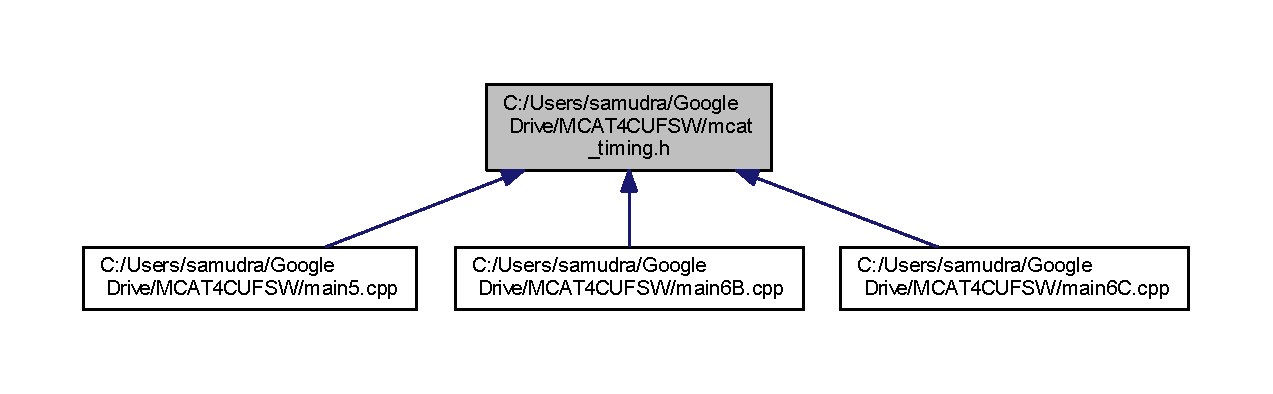
\includegraphics[width=350pt]{mcat__timing_8h__dep__incl}
\end{center}
\end{figure}
\subsection*{Variables}
\begin{DoxyCompactItemize}
\item 
int \hyperlink{mcat__timing_8h_ace0b5394e25ed3b3323ca9163ab156d4}{T\+S\+R\+D} = 623
\item 
int \hyperlink{mcat__timing_8h_a1d447a6214fe551ca32f2879ea0b8d08}{T\+S\+R} = \hyperlink{mcat__timing_8h_ace0b5394e25ed3b3323ca9163ab156d4}{T\+S\+R\+D}
\item 
int \hyperlink{mcat__timing_8h_a613c70f84959e74db7e193a3d218bab2}{P\+P\+U\+\_\+\+S\+A\+F\+E\+\_\+\+O\+P\+S\+\_\+\+M\+I\+N} = 1
\item 
int \hyperlink{mcat__timing_8h_ad9c2c893122d53ec776cbfe933e7813b}{P\+P\+U\+\_\+\+S\+A\+F\+E\+\_\+\+O\+P\+S\+\_\+\+M\+A\+X} = 50
\item 
long \hyperlink{mcat__timing_8h_a27dd6f9a73f9f0326fb12550ab48b3d2}{E\+O\+C\+C\+\_\+array} \mbox{[}50\mbox{]}
\item 
int \hyperlink{mcat__timing_8h_a8185679b1120bd514c22e80e5aa9f7e7}{M\+C\+H\+C\+D} = 0
\item 
int \hyperlink{mcat__timing_8h_a3c336bbdab01b16af648745188846f65}{T\+P\+H\+C\+D} = 14
\item 
int \hyperlink{mcat__timing_8h_a27f15a79275c07b4c5caf220332ec81d}{T\+P\+L\+C\+D} = 29
\item 
int \hyperlink{mcat__timing_8h_a39606011f61540356781c166e4543593}{M\+C\+L\+C\+D} = 44
\item 
int \hyperlink{mcat__timing_8h_a453172ff9aed0d75ba17aa923b0b065e}{E\+O\+C\+C\+D} = 99954
\item 
int \hyperlink{mcat__timing_8h_a5f31c9f57fb2680de665ab92db5a6818}{E\+O\+C\+C\+D50} = \hyperlink{mcat__timing_8h_a27dd6f9a73f9f0326fb12550ab48b3d2}{E\+O\+C\+C\+\_\+array}\mbox{[}50-\/1\mbox{]}
\item 
int \hyperlink{mcat__timing_8h_a7e1cab479edcac221a1991d2cf7e165a}{E\+O\+C\+C\+D10} = \hyperlink{mcat__timing_8h_a27dd6f9a73f9f0326fb12550ab48b3d2}{E\+O\+C\+C\+\_\+array}\mbox{[}10-\/1\mbox{]}
\item 
int \hyperlink{mcat__timing_8h_aeb9c4bc70e53edb70bb15b0af6ebf5cf}{M\+C\+H\+C} = \hyperlink{mcat__timing_8h_a8185679b1120bd514c22e80e5aa9f7e7}{M\+C\+H\+C\+D}
\item 
int \hyperlink{mcat__timing_8h_a59eec089e1d6c321803517582f87734c}{T\+P\+H\+C} = \hyperlink{mcat__timing_8h_a3c336bbdab01b16af648745188846f65}{T\+P\+H\+C\+D}
\item 
int \hyperlink{mcat__timing_8h_afd2f4d17369e48a88e0924b0546d1ab7}{T\+P\+L\+C} = \hyperlink{mcat__timing_8h_a27f15a79275c07b4c5caf220332ec81d}{T\+P\+L\+C\+D}
\item 
int \hyperlink{mcat__timing_8h_a2a39cac3041faed9db66c783197ccecb}{M\+C\+L\+C} = \hyperlink{mcat__timing_8h_a39606011f61540356781c166e4543593}{M\+C\+L\+C\+D}
\item 
int \hyperlink{mcat__timing_8h_a23b84a5df83e6f9a3b681ac4f642215b}{E\+O\+C\+C} = \hyperlink{mcat__timing_8h_a453172ff9aed0d75ba17aa923b0b065e}{E\+O\+C\+C\+D}
\end{DoxyCompactItemize}


\subsection{Variable Documentation}
\hypertarget{mcat__timing_8h_a23b84a5df83e6f9a3b681ac4f642215b}{}\index{mcat\+\_\+timing.\+h@{mcat\+\_\+timing.\+h}!E\+O\+C\+C@{E\+O\+C\+C}}
\index{E\+O\+C\+C@{E\+O\+C\+C}!mcat\+\_\+timing.\+h@{mcat\+\_\+timing.\+h}}
\subsubsection[{E\+O\+C\+C}]{\setlength{\rightskip}{0pt plus 5cm}int E\+O\+C\+C = {\bf E\+O\+C\+C\+D}}\label{mcat__timing_8h_a23b84a5df83e6f9a3b681ac4f642215b}


Definition at line 42 of file mcat\+\_\+timing.\+h.

\hypertarget{mcat__timing_8h_a27dd6f9a73f9f0326fb12550ab48b3d2}{}\index{mcat\+\_\+timing.\+h@{mcat\+\_\+timing.\+h}!E\+O\+C\+C\+\_\+array@{E\+O\+C\+C\+\_\+array}}
\index{E\+O\+C\+C\+\_\+array@{E\+O\+C\+C\+\_\+array}!mcat\+\_\+timing.\+h@{mcat\+\_\+timing.\+h}}
\subsubsection[{E\+O\+C\+C\+\_\+array}]{\setlength{\rightskip}{0pt plus 5cm}long E\+O\+C\+C\+\_\+array\mbox{[}50\mbox{]}}\label{mcat__timing_8h_a27dd6f9a73f9f0326fb12550ab48b3d2}
{\bfseries Initial value\+:}
\begin{DoxyCode}
= \{
        99954, 49954, 33288, 24954, 19954, 16621, 14240, 12454, 11065, 9954,
        9045, 8288, 7647, 7097, 6621, 6204, 5837, 5510, 5218, 4954,
        4716, 4500, 4302, 4121, 3954, 3801, 3658, 3526, 3403, 3288,
        3180, 3079, 2985, 2896, 2812, 2732, 2657, 2586, 2518, 2454,
        2393, 2335, 2280, 2227, 2177, 2128, 2082, 2038, 1995, 1954
\}
\end{DoxyCode}


Definition at line 19 of file mcat\+\_\+timing.\+h.

\hypertarget{mcat__timing_8h_a453172ff9aed0d75ba17aa923b0b065e}{}\index{mcat\+\_\+timing.\+h@{mcat\+\_\+timing.\+h}!E\+O\+C\+C\+D@{E\+O\+C\+C\+D}}
\index{E\+O\+C\+C\+D@{E\+O\+C\+C\+D}!mcat\+\_\+timing.\+h@{mcat\+\_\+timing.\+h}}
\subsubsection[{E\+O\+C\+C\+D}]{\setlength{\rightskip}{0pt plus 5cm}int E\+O\+C\+C\+D = 99954}\label{mcat__timing_8h_a453172ff9aed0d75ba17aa923b0b065e}


Definition at line 33 of file mcat\+\_\+timing.\+h.

\hypertarget{mcat__timing_8h_a7e1cab479edcac221a1991d2cf7e165a}{}\index{mcat\+\_\+timing.\+h@{mcat\+\_\+timing.\+h}!E\+O\+C\+C\+D10@{E\+O\+C\+C\+D10}}
\index{E\+O\+C\+C\+D10@{E\+O\+C\+C\+D10}!mcat\+\_\+timing.\+h@{mcat\+\_\+timing.\+h}}
\subsubsection[{E\+O\+C\+C\+D10}]{\setlength{\rightskip}{0pt plus 5cm}int E\+O\+C\+C\+D10 = {\bf E\+O\+C\+C\+\_\+array}\mbox{[}10-\/1\mbox{]}}\label{mcat__timing_8h_a7e1cab479edcac221a1991d2cf7e165a}


Definition at line 35 of file mcat\+\_\+timing.\+h.

\hypertarget{mcat__timing_8h_a5f31c9f57fb2680de665ab92db5a6818}{}\index{mcat\+\_\+timing.\+h@{mcat\+\_\+timing.\+h}!E\+O\+C\+C\+D50@{E\+O\+C\+C\+D50}}
\index{E\+O\+C\+C\+D50@{E\+O\+C\+C\+D50}!mcat\+\_\+timing.\+h@{mcat\+\_\+timing.\+h}}
\subsubsection[{E\+O\+C\+C\+D50}]{\setlength{\rightskip}{0pt plus 5cm}int E\+O\+C\+C\+D50 = {\bf E\+O\+C\+C\+\_\+array}\mbox{[}50-\/1\mbox{]}}\label{mcat__timing_8h_a5f31c9f57fb2680de665ab92db5a6818}


Definition at line 34 of file mcat\+\_\+timing.\+h.

\hypertarget{mcat__timing_8h_aeb9c4bc70e53edb70bb15b0af6ebf5cf}{}\index{mcat\+\_\+timing.\+h@{mcat\+\_\+timing.\+h}!M\+C\+H\+C@{M\+C\+H\+C}}
\index{M\+C\+H\+C@{M\+C\+H\+C}!mcat\+\_\+timing.\+h@{mcat\+\_\+timing.\+h}}
\subsubsection[{M\+C\+H\+C}]{\setlength{\rightskip}{0pt plus 5cm}int M\+C\+H\+C = {\bf M\+C\+H\+C\+D}}\label{mcat__timing_8h_aeb9c4bc70e53edb70bb15b0af6ebf5cf}


Definition at line 38 of file mcat\+\_\+timing.\+h.

\hypertarget{mcat__timing_8h_a8185679b1120bd514c22e80e5aa9f7e7}{}\index{mcat\+\_\+timing.\+h@{mcat\+\_\+timing.\+h}!M\+C\+H\+C\+D@{M\+C\+H\+C\+D}}
\index{M\+C\+H\+C\+D@{M\+C\+H\+C\+D}!mcat\+\_\+timing.\+h@{mcat\+\_\+timing.\+h}}
\subsubsection[{M\+C\+H\+C\+D}]{\setlength{\rightskip}{0pt plus 5cm}int M\+C\+H\+C\+D = 0}\label{mcat__timing_8h_a8185679b1120bd514c22e80e5aa9f7e7}


Definition at line 28 of file mcat\+\_\+timing.\+h.

\hypertarget{mcat__timing_8h_a2a39cac3041faed9db66c783197ccecb}{}\index{mcat\+\_\+timing.\+h@{mcat\+\_\+timing.\+h}!M\+C\+L\+C@{M\+C\+L\+C}}
\index{M\+C\+L\+C@{M\+C\+L\+C}!mcat\+\_\+timing.\+h@{mcat\+\_\+timing.\+h}}
\subsubsection[{M\+C\+L\+C}]{\setlength{\rightskip}{0pt plus 5cm}int M\+C\+L\+C = {\bf M\+C\+L\+C\+D}}\label{mcat__timing_8h_a2a39cac3041faed9db66c783197ccecb}


Definition at line 41 of file mcat\+\_\+timing.\+h.

\hypertarget{mcat__timing_8h_a39606011f61540356781c166e4543593}{}\index{mcat\+\_\+timing.\+h@{mcat\+\_\+timing.\+h}!M\+C\+L\+C\+D@{M\+C\+L\+C\+D}}
\index{M\+C\+L\+C\+D@{M\+C\+L\+C\+D}!mcat\+\_\+timing.\+h@{mcat\+\_\+timing.\+h}}
\subsubsection[{M\+C\+L\+C\+D}]{\setlength{\rightskip}{0pt plus 5cm}int M\+C\+L\+C\+D = 44}\label{mcat__timing_8h_a39606011f61540356781c166e4543593}


Definition at line 32 of file mcat\+\_\+timing.\+h.

\hypertarget{mcat__timing_8h_ad9c2c893122d53ec776cbfe933e7813b}{}\index{mcat\+\_\+timing.\+h@{mcat\+\_\+timing.\+h}!P\+P\+U\+\_\+\+S\+A\+F\+E\+\_\+\+O\+P\+S\+\_\+\+M\+A\+X@{P\+P\+U\+\_\+\+S\+A\+F\+E\+\_\+\+O\+P\+S\+\_\+\+M\+A\+X}}
\index{P\+P\+U\+\_\+\+S\+A\+F\+E\+\_\+\+O\+P\+S\+\_\+\+M\+A\+X@{P\+P\+U\+\_\+\+S\+A\+F\+E\+\_\+\+O\+P\+S\+\_\+\+M\+A\+X}!mcat\+\_\+timing.\+h@{mcat\+\_\+timing.\+h}}
\subsubsection[{P\+P\+U\+\_\+\+S\+A\+F\+E\+\_\+\+O\+P\+S\+\_\+\+M\+A\+X}]{\setlength{\rightskip}{0pt plus 5cm}int P\+P\+U\+\_\+\+S\+A\+F\+E\+\_\+\+O\+P\+S\+\_\+\+M\+A\+X = 50}\label{mcat__timing_8h_ad9c2c893122d53ec776cbfe933e7813b}


Definition at line 16 of file mcat\+\_\+timing.\+h.

\hypertarget{mcat__timing_8h_a613c70f84959e74db7e193a3d218bab2}{}\index{mcat\+\_\+timing.\+h@{mcat\+\_\+timing.\+h}!P\+P\+U\+\_\+\+S\+A\+F\+E\+\_\+\+O\+P\+S\+\_\+\+M\+I\+N@{P\+P\+U\+\_\+\+S\+A\+F\+E\+\_\+\+O\+P\+S\+\_\+\+M\+I\+N}}
\index{P\+P\+U\+\_\+\+S\+A\+F\+E\+\_\+\+O\+P\+S\+\_\+\+M\+I\+N@{P\+P\+U\+\_\+\+S\+A\+F\+E\+\_\+\+O\+P\+S\+\_\+\+M\+I\+N}!mcat\+\_\+timing.\+h@{mcat\+\_\+timing.\+h}}
\subsubsection[{P\+P\+U\+\_\+\+S\+A\+F\+E\+\_\+\+O\+P\+S\+\_\+\+M\+I\+N}]{\setlength{\rightskip}{0pt plus 5cm}int P\+P\+U\+\_\+\+S\+A\+F\+E\+\_\+\+O\+P\+S\+\_\+\+M\+I\+N = 1}\label{mcat__timing_8h_a613c70f84959e74db7e193a3d218bab2}


Definition at line 15 of file mcat\+\_\+timing.\+h.

\hypertarget{mcat__timing_8h_a59eec089e1d6c321803517582f87734c}{}\index{mcat\+\_\+timing.\+h@{mcat\+\_\+timing.\+h}!T\+P\+H\+C@{T\+P\+H\+C}}
\index{T\+P\+H\+C@{T\+P\+H\+C}!mcat\+\_\+timing.\+h@{mcat\+\_\+timing.\+h}}
\subsubsection[{T\+P\+H\+C}]{\setlength{\rightskip}{0pt plus 5cm}int T\+P\+H\+C = {\bf T\+P\+H\+C\+D}}\label{mcat__timing_8h_a59eec089e1d6c321803517582f87734c}


Definition at line 39 of file mcat\+\_\+timing.\+h.

\hypertarget{mcat__timing_8h_a3c336bbdab01b16af648745188846f65}{}\index{mcat\+\_\+timing.\+h@{mcat\+\_\+timing.\+h}!T\+P\+H\+C\+D@{T\+P\+H\+C\+D}}
\index{T\+P\+H\+C\+D@{T\+P\+H\+C\+D}!mcat\+\_\+timing.\+h@{mcat\+\_\+timing.\+h}}
\subsubsection[{T\+P\+H\+C\+D}]{\setlength{\rightskip}{0pt plus 5cm}int T\+P\+H\+C\+D = 14}\label{mcat__timing_8h_a3c336bbdab01b16af648745188846f65}


Definition at line 29 of file mcat\+\_\+timing.\+h.

\hypertarget{mcat__timing_8h_afd2f4d17369e48a88e0924b0546d1ab7}{}\index{mcat\+\_\+timing.\+h@{mcat\+\_\+timing.\+h}!T\+P\+L\+C@{T\+P\+L\+C}}
\index{T\+P\+L\+C@{T\+P\+L\+C}!mcat\+\_\+timing.\+h@{mcat\+\_\+timing.\+h}}
\subsubsection[{T\+P\+L\+C}]{\setlength{\rightskip}{0pt plus 5cm}int T\+P\+L\+C = {\bf T\+P\+L\+C\+D}}\label{mcat__timing_8h_afd2f4d17369e48a88e0924b0546d1ab7}


Definition at line 40 of file mcat\+\_\+timing.\+h.

\hypertarget{mcat__timing_8h_a27f15a79275c07b4c5caf220332ec81d}{}\index{mcat\+\_\+timing.\+h@{mcat\+\_\+timing.\+h}!T\+P\+L\+C\+D@{T\+P\+L\+C\+D}}
\index{T\+P\+L\+C\+D@{T\+P\+L\+C\+D}!mcat\+\_\+timing.\+h@{mcat\+\_\+timing.\+h}}
\subsubsection[{T\+P\+L\+C\+D}]{\setlength{\rightskip}{0pt plus 5cm}int T\+P\+L\+C\+D = 29}\label{mcat__timing_8h_a27f15a79275c07b4c5caf220332ec81d}


Definition at line 30 of file mcat\+\_\+timing.\+h.

\hypertarget{mcat__timing_8h_a1d447a6214fe551ca32f2879ea0b8d08}{}\index{mcat\+\_\+timing.\+h@{mcat\+\_\+timing.\+h}!T\+S\+R@{T\+S\+R}}
\index{T\+S\+R@{T\+S\+R}!mcat\+\_\+timing.\+h@{mcat\+\_\+timing.\+h}}
\subsubsection[{T\+S\+R}]{\setlength{\rightskip}{0pt plus 5cm}int T\+S\+R = {\bf T\+S\+R\+D}}\label{mcat__timing_8h_a1d447a6214fe551ca32f2879ea0b8d08}


Definition at line 12 of file mcat\+\_\+timing.\+h.

\hypertarget{mcat__timing_8h_ace0b5394e25ed3b3323ca9163ab156d4}{}\index{mcat\+\_\+timing.\+h@{mcat\+\_\+timing.\+h}!T\+S\+R\+D@{T\+S\+R\+D}}
\index{T\+S\+R\+D@{T\+S\+R\+D}!mcat\+\_\+timing.\+h@{mcat\+\_\+timing.\+h}}
\subsubsection[{T\+S\+R\+D}]{\setlength{\rightskip}{0pt plus 5cm}int T\+S\+R\+D = 623}\label{mcat__timing_8h_ace0b5394e25ed3b3323ca9163ab156d4}


Definition at line 11 of file mcat\+\_\+timing.\+h.


\hypertarget{mcatsubsystemconfig_8h}{}\section{C\+:/\+Users/samudra/\+Google Drive/\+M\+C\+A\+T4\+C\+U\+F\+S\+W/mcatsubsystemconfig.h File Reference}
\label{mcatsubsystemconfig_8h}\index{C\+:/\+Users/samudra/\+Google Drive/\+M\+C\+A\+T4\+C\+U\+F\+S\+W/mcatsubsystemconfig.\+h@{C\+:/\+Users/samudra/\+Google Drive/\+M\+C\+A\+T4\+C\+U\+F\+S\+W/mcatsubsystemconfig.\+h}}
{\ttfamily \#include $<$iostream$>$}\\*
{\ttfamily \#include $<$iomanip$>$}\\*
{\ttfamily \#include $<$string$>$}\\*
Include dependency graph for mcatsubsystemconfig.\+h\+:
\nopagebreak
\begin{figure}[H]
\begin{center}
\leavevmode
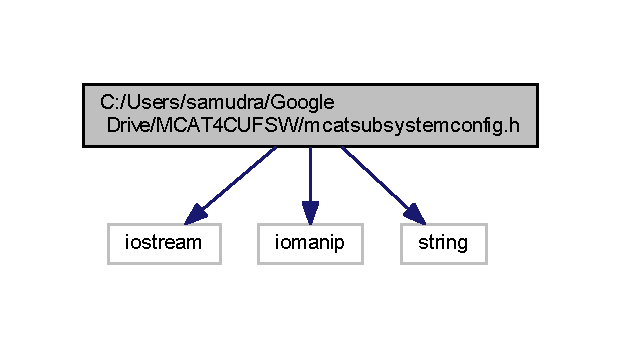
\includegraphics[width=298pt]{mcatsubsystemconfig_8h__incl}
\end{center}
\end{figure}
\subsection*{Macros}
\begin{DoxyCompactItemize}
\item 
\#define \hyperlink{mcatsubsystemconfig_8h_a8fe248bd745b90e2bfe94d8c5fce0a53}{C\+U\+\_\+\+I2\+C\+\_\+\+S\+L\+A\+V\+E\+\_\+\+A\+D\+D\+R}~0x26
\item 
\#define \hyperlink{mcatsubsystemconfig_8h_a65b537eaba53f6a2e9baa86e843aa393}{T\+E\+S\+T\+B\+U\+S\+\_\+\+I2\+C\+\_\+\+S\+L\+A\+V\+E\+\_\+\+A\+D\+D\+R}~0x24
\item 
\#define \hyperlink{mcatsubsystemconfig_8h_ad96b6d31ce20f216b55fc2a32ac4f479}{M\+C\+A\+T\+\_\+\+I2\+C\+\_\+\+C\+M\+D\+\_\+\+P\+A\+C\+K\+E\+T\+\_\+\+L\+E\+N}~34
\item 
\#define \hyperlink{mcatsubsystemconfig_8h_a57cc7693b03a0bf2eaf6c0e5d97b68e2}{M\+C\+A\+T\+\_\+\+C\+M\+D\+\_\+\+G\+O\+\_\+\+I\+D\+L\+E\+\_\+\+M\+O\+D\+E}~\textquotesingle{}I\+D\+L\+E\textquotesingle{}
\item 
\#define \hyperlink{mcatsubsystemconfig_8h_a67c451cf73d565d2d941eacc6f23419f}{M\+C\+A\+T\+\_\+\+C\+M\+D\+\_\+\+G\+O\+\_\+\+S\+T\+A\+N\+D\+B\+Y\+\_\+\+M\+O\+D\+E}~\char`\"{}S\+T\+B\+Y\char`\"{}
\item 
\#define \hyperlink{mcatsubsystemconfig_8h_a7867df8655a6f6639b86efaef48fcf58}{M\+C\+A\+T\+\_\+\+C\+M\+D\+\_\+\+E\+N\+A\+B\+L\+E\+\_\+\+T\+R\+I\+G\+G\+E\+R\+\_\+\+P\+U\+L\+S\+E\+S}~\char`\"{}E\+N\+T\+P\char`\"{}
\item 
\#define \hyperlink{mcatsubsystemconfig_8h_a6840ce2ca25277e0668c39cff15ae22a}{M\+C\+A\+T\+\_\+\+C\+M\+D\+\_\+\+E\+N\+A\+B\+L\+E\+\_\+\+T\+H\+R\+U\+S\+T\+E\+R\+\_\+\+C\+H\+A\+N\+N\+E\+L\+S}~\char`\"{}E\+N\+T\+C\char`\"{}
\item 
\#define \hyperlink{mcatsubsystemconfig_8h_acfb56a40e9b394d7ede3c89bc94e68dc}{M\+C\+A\+T\+\_\+\+C\+M\+D\+\_\+\+D\+I\+S\+A\+B\+L\+E\+\_\+\+T\+H\+R\+U\+S\+T\+E\+R\+\_\+\+C\+H\+A\+N\+N\+E\+L\+S}~\char`\"{}D\+I\+T\+C\char`\"{}
\item 
\#define \hyperlink{mcatsubsystemconfig_8h_af8b355b0055a53173a5f6e62c13d502b}{M\+C\+A\+T\+\_\+\+C\+M\+D\+\_\+\+D\+I\+S\+A\+B\+L\+E\+\_\+\+T\+R\+I\+G\+G\+E\+R\+\_\+\+P\+U\+L\+S\+E\+S}~\char`\"{}D\+I\+T\+P\char`\"{}
\item 
\#define \hyperlink{mcatsubsystemconfig_8h_a24afa2de64c6357b182727627a6c85c7}{M\+C\+A\+T\+\_\+\+C\+M\+D\+\_\+\+Q\+U\+E\+R\+Y\+\_\+\+T\+L\+M\+\_\+\+S\+I\+N\+G\+L\+E}~\char`\"{}T\+L\+M1\char`\"{}
\item 
\#define \hyperlink{mcatsubsystemconfig_8h_aec0b77609021421714530871dba76998}{M\+C\+A\+T\+\_\+\+C\+M\+D\+\_\+\+Q\+U\+E\+R\+Y\+\_\+\+T\+L\+M\+\_\+\+C\+O\+N\+T\+I\+N\+U\+O\+U\+S}~\char`\"{}T\+L\+M\+C\char`\"{}
\item 
\#define \hyperlink{mcatsubsystemconfig_8h_a322065545a199be4e4f2ddb7b8b29979}{M\+C\+A\+T\+\_\+\+C\+M\+D\+\_\+\+Q\+U\+E\+R\+Y\+\_\+\+T\+L\+M\+\_\+\+S\+T\+O\+P}~\char`\"{}T\+L\+M\+S\char`\"{}
\item 
\#define \hyperlink{mcatsubsystemconfig_8h_a14afd22fc615cabe292eecf46c7de0bb}{B\+U\+I\+L\+D\+\_\+\+M\+A\+J\+O\+R}~\char`\"{}5\char`\"{}
\item 
\#define \hyperlink{mcatsubsystemconfig_8h_a6ecb2f775a2f51fecce9a21ab897daf8}{B\+U\+I\+L\+D\+\_\+\+M\+I\+N\+O\+R}~\char`\"{}A\char`\"{}
\item 
\#define \hyperlink{mcatsubsystemconfig_8h_a0df90ddf0b04f017fb087e7196e784d1}{V\+E\+R\+S\+I\+O\+N\+\_\+\+L\+E\+N}~10
\item 
\#define \hyperlink{mcatsubsystemconfig_8h_a50e40f98b0a2e1338e46f50d178434c1}{B\+U\+I\+L\+D\+\_\+\+T\+I\+M\+E\+S\+T\+A\+M\+P}~\char`\"{}201409251844\char`\"{}
\item 
\#define \hyperlink{mcatsubsystemconfig_8h_aa83c1f4aafa1a8610d231d8e2721d4e0}{B\+U\+I\+L\+D\+\_\+\+A\+P\+P\+\_\+\+T\+A\+S\+K\+M\+O\+N}~\char`\"{}M2\+C\+U-\/4\+G\char`\"{}
\item 
\#define \hyperlink{mcatsubsystemconfig_8h_af20537a0b4c7ffdf9df866736be554ab}{B\+U\+I\+L\+D\+\_\+\+A\+P\+P\+\_\+\+T\+I\+T\+L\+E}~\char`\"{}Micro-\/Cathode Arc Thruster 2-\/Ch Control Unit -\/ Remote Test Program\char`\"{}
\item 
\#define \hyperlink{mcatsubsystemconfig_8h_ad4e0899c1923f08b95540907308812f2}{M\+C\+A\+T\+\_\+\+C\+M\+D\+\_\+\+V\+E\+R\+S\+I\+O\+N\+\_\+\+L\+E\+N}~2
\item 
\#define \hyperlink{mcatsubsystemconfig_8h_ae70b0b99cdaec02c82b324f763845eb0}{M\+C\+A\+T\+\_\+\+C\+M\+D\+\_\+\+M\+O\+D\+E\+\_\+\+L\+E\+N}~3
\item 
\#define \hyperlink{mcatsubsystemconfig_8h_a8679e50fe282fd32fd9bbde8f892020b}{D\+E\+F\+\_\+\+C\+M\+D\+\_\+\+V\+E\+R\+S\+I\+O\+N}~\char`\"{}V1\char`\"{}
\item 
\#define \hyperlink{mcatsubsystemconfig_8h_a33dfdd1381b4c43471adde87a9bf01a8}{L\+E\+N\+\_\+\+C\+M\+D\+\_\+\+C\+U}
\item 
\#define \hyperlink{mcatsubsystemconfig_8h_a585d7d23eb9f3b097c0202f583fb14f1}{L\+E\+N\+\_\+\+C\+M\+D\+\_\+\+C\+U\+\_\+\+B\+I\+T\+E}~1
\item 
\#define \hyperlink{mcatsubsystemconfig_8h_a3044761c407d1976b979345f51cbfbb5}{L\+E\+N\+\_\+\+C\+M\+D\+\_\+\+C\+U\+\_\+\+T\+I\+M\+E}~4
\item 
\#define \hyperlink{mcatsubsystemconfig_8h_a2f6ba47c9e2ec0f6cbdc5917fa9380ec}{M\+O\+D\+E\+\_\+\+C\+H\+A\+N\+G\+E\+\_\+\+T\+O\+\_\+\+I\+D\+L\+E}~\char`\"{}M11\char`\"{}
\item 
\#define \hyperlink{mcatsubsystemconfig_8h_ac8626c3e2d8ee55d1faa67de3294de79}{M\+O\+D\+E\+\_\+\+C\+H\+A\+N\+G\+E\+\_\+\+T\+O\+\_\+\+S\+T\+A\+N\+D\+B\+Y}~\char`\"{}M21\char`\"{}
\item 
\#define \hyperlink{mcatsubsystemconfig_8h_a4df7cee39c3aaf21bffffd6aa70b41a1}{D\+E\+F\+\_\+\+C\+M\+D\+\_\+\+C\+U\+\_\+\+T\+I\+M\+E}~\char`\"{}0000\char`\"{}
\item 
\#define \hyperlink{mcatsubsystemconfig_8h_a8248495645b5382783a9889f265082be}{L\+E\+N\+\_\+\+C\+M\+D\+\_\+\+P\+M}~2
\item 
\#define \hyperlink{mcatsubsystemconfig_8h_a2d09aee307eabf8f956f8e319d75e069}{L\+E\+N\+\_\+\+C\+M\+D\+\_\+\+P\+M\+\_\+\+B\+I\+T\+E}
\item 
\#define \hyperlink{mcatsubsystemconfig_8h_a05d71f031ba8c1e6f695068cd15ff692}{L\+E\+N\+\_\+\+C\+M\+D\+\_\+\+I\+P\+D}~2
\item 
\#define \hyperlink{mcatsubsystemconfig_8h_a8f01dd1656644ca257b91c47798c06ef}{L\+E\+N\+\_\+\+C\+M\+D\+\_\+\+I\+P\+D\+\_\+\+B\+I\+T\+E}
\item 
\#define \hyperlink{mcatsubsystemconfig_8h_a4710b766ad9e2d466faa237d9fe152d2}{L\+E\+N\+\_\+\+C\+M\+D\+\_\+\+P\+P\+U}~2
\item 
\#define \hyperlink{mcatsubsystemconfig_8h_ade96c16c6780770b13b4dbe71e8023f7}{L\+E\+N\+\_\+\+C\+M\+D\+\_\+\+P\+P\+U\+\_\+\+B\+I\+T\+E}
\item 
\#define \hyperlink{mcatsubsystemconfig_8h_af672fea135e3337d978be770ac47caea}{L\+E\+N\+\_\+\+C\+M\+D\+\_\+\+M\+N\+P\+S}~2
\item 
\#define \hyperlink{mcatsubsystemconfig_8h_adba8a63a494d31864c7893c9210318c6}{L\+E\+N\+\_\+\+C\+M\+D\+\_\+\+M\+N\+P\+S\+\_\+\+B\+I\+T\+E}
\item 
\#define \hyperlink{mcatsubsystemconfig_8h_a7d6a25cda8dea3de3291b73f61992902}{L\+E\+N\+\_\+\+C\+M\+D\+\_\+\+S\+E\+N\+S\+O\+R\+S}~2
\item 
\#define \hyperlink{mcatsubsystemconfig_8h_a2c0d1a6640b07b5027cf612eb2929e3d}{L\+E\+N\+\_\+\+C\+M\+D\+\_\+\+S\+E\+N\+S\+O\+R\+S\+\_\+\+B\+I\+T\+E}
\item 
\#define \hyperlink{mcatsubsystemconfig_8h_a322065545a199be4e4f2ddb7b8b29979}{M\+C\+A\+T\+\_\+\+C\+M\+D\+\_\+\+Q\+U\+E\+R\+Y\+\_\+\+T\+L\+M\+\_\+\+S\+T\+O\+P}~\char`\"{}T\+L\+M\+S\char`\"{}
\end{DoxyCompactItemize}
\subsection*{Variables}
\begin{DoxyCompactItemize}
\item 
char \hyperlink{mcatsubsystemconfig_8h_abc81884c63372e50da2e117e75a92aba}{M\+C\+A\+T\+\_\+\+C\+M\+D} \mbox{[}4\mbox{]}
\item 
char \hyperlink{mcatsubsystemconfig_8h_a928764f51c539f07225048c5a648ecf2}{M\+C\+A\+T\+\_\+\+C\+M\+D\+\_\+\+Q\+U\+E\+R\+Y} \mbox{[}4\mbox{]}
\end{DoxyCompactItemize}


\subsection{Macro Definition Documentation}
\hypertarget{mcatsubsystemconfig_8h_aa83c1f4aafa1a8610d231d8e2721d4e0}{}\index{mcatsubsystemconfig.\+h@{mcatsubsystemconfig.\+h}!B\+U\+I\+L\+D\+\_\+\+A\+P\+P\+\_\+\+T\+A\+S\+K\+M\+O\+N@{B\+U\+I\+L\+D\+\_\+\+A\+P\+P\+\_\+\+T\+A\+S\+K\+M\+O\+N}}
\index{B\+U\+I\+L\+D\+\_\+\+A\+P\+P\+\_\+\+T\+A\+S\+K\+M\+O\+N@{B\+U\+I\+L\+D\+\_\+\+A\+P\+P\+\_\+\+T\+A\+S\+K\+M\+O\+N}!mcatsubsystemconfig.\+h@{mcatsubsystemconfig.\+h}}
\subsubsection[{B\+U\+I\+L\+D\+\_\+\+A\+P\+P\+\_\+\+T\+A\+S\+K\+M\+O\+N}]{\setlength{\rightskip}{0pt plus 5cm}\#define B\+U\+I\+L\+D\+\_\+\+A\+P\+P\+\_\+\+T\+A\+S\+K\+M\+O\+N~\char`\"{}M2\+C\+U-\/4\+G\char`\"{}}\label{mcatsubsystemconfig_8h_aa83c1f4aafa1a8610d231d8e2721d4e0}


Definition at line 49 of file mcatsubsystemconfig.\+h.

\hypertarget{mcatsubsystemconfig_8h_af20537a0b4c7ffdf9df866736be554ab}{}\index{mcatsubsystemconfig.\+h@{mcatsubsystemconfig.\+h}!B\+U\+I\+L\+D\+\_\+\+A\+P\+P\+\_\+\+T\+I\+T\+L\+E@{B\+U\+I\+L\+D\+\_\+\+A\+P\+P\+\_\+\+T\+I\+T\+L\+E}}
\index{B\+U\+I\+L\+D\+\_\+\+A\+P\+P\+\_\+\+T\+I\+T\+L\+E@{B\+U\+I\+L\+D\+\_\+\+A\+P\+P\+\_\+\+T\+I\+T\+L\+E}!mcatsubsystemconfig.\+h@{mcatsubsystemconfig.\+h}}
\subsubsection[{B\+U\+I\+L\+D\+\_\+\+A\+P\+P\+\_\+\+T\+I\+T\+L\+E}]{\setlength{\rightskip}{0pt plus 5cm}\#define B\+U\+I\+L\+D\+\_\+\+A\+P\+P\+\_\+\+T\+I\+T\+L\+E~\char`\"{}Micro-\/Cathode Arc Thruster 2-\/Ch Control Unit -\/ Remote Test Program\char`\"{}}\label{mcatsubsystemconfig_8h_af20537a0b4c7ffdf9df866736be554ab}


Definition at line 50 of file mcatsubsystemconfig.\+h.

\hypertarget{mcatsubsystemconfig_8h_a14afd22fc615cabe292eecf46c7de0bb}{}\index{mcatsubsystemconfig.\+h@{mcatsubsystemconfig.\+h}!B\+U\+I\+L\+D\+\_\+\+M\+A\+J\+O\+R@{B\+U\+I\+L\+D\+\_\+\+M\+A\+J\+O\+R}}
\index{B\+U\+I\+L\+D\+\_\+\+M\+A\+J\+O\+R@{B\+U\+I\+L\+D\+\_\+\+M\+A\+J\+O\+R}!mcatsubsystemconfig.\+h@{mcatsubsystemconfig.\+h}}
\subsubsection[{B\+U\+I\+L\+D\+\_\+\+M\+A\+J\+O\+R}]{\setlength{\rightskip}{0pt plus 5cm}\#define B\+U\+I\+L\+D\+\_\+\+M\+A\+J\+O\+R~\char`\"{}5\char`\"{}}\label{mcatsubsystemconfig_8h_a14afd22fc615cabe292eecf46c7de0bb}


Definition at line 44 of file mcatsubsystemconfig.\+h.

\hypertarget{mcatsubsystemconfig_8h_a6ecb2f775a2f51fecce9a21ab897daf8}{}\index{mcatsubsystemconfig.\+h@{mcatsubsystemconfig.\+h}!B\+U\+I\+L\+D\+\_\+\+M\+I\+N\+O\+R@{B\+U\+I\+L\+D\+\_\+\+M\+I\+N\+O\+R}}
\index{B\+U\+I\+L\+D\+\_\+\+M\+I\+N\+O\+R@{B\+U\+I\+L\+D\+\_\+\+M\+I\+N\+O\+R}!mcatsubsystemconfig.\+h@{mcatsubsystemconfig.\+h}}
\subsubsection[{B\+U\+I\+L\+D\+\_\+\+M\+I\+N\+O\+R}]{\setlength{\rightskip}{0pt plus 5cm}\#define B\+U\+I\+L\+D\+\_\+\+M\+I\+N\+O\+R~\char`\"{}A\char`\"{}}\label{mcatsubsystemconfig_8h_a6ecb2f775a2f51fecce9a21ab897daf8}


Definition at line 45 of file mcatsubsystemconfig.\+h.

\hypertarget{mcatsubsystemconfig_8h_a50e40f98b0a2e1338e46f50d178434c1}{}\index{mcatsubsystemconfig.\+h@{mcatsubsystemconfig.\+h}!B\+U\+I\+L\+D\+\_\+\+T\+I\+M\+E\+S\+T\+A\+M\+P@{B\+U\+I\+L\+D\+\_\+\+T\+I\+M\+E\+S\+T\+A\+M\+P}}
\index{B\+U\+I\+L\+D\+\_\+\+T\+I\+M\+E\+S\+T\+A\+M\+P@{B\+U\+I\+L\+D\+\_\+\+T\+I\+M\+E\+S\+T\+A\+M\+P}!mcatsubsystemconfig.\+h@{mcatsubsystemconfig.\+h}}
\subsubsection[{B\+U\+I\+L\+D\+\_\+\+T\+I\+M\+E\+S\+T\+A\+M\+P}]{\setlength{\rightskip}{0pt plus 5cm}\#define B\+U\+I\+L\+D\+\_\+\+T\+I\+M\+E\+S\+T\+A\+M\+P~\char`\"{}201409251844\char`\"{}}\label{mcatsubsystemconfig_8h_a50e40f98b0a2e1338e46f50d178434c1}


Definition at line 48 of file mcatsubsystemconfig.\+h.

\hypertarget{mcatsubsystemconfig_8h_a8fe248bd745b90e2bfe94d8c5fce0a53}{}\index{mcatsubsystemconfig.\+h@{mcatsubsystemconfig.\+h}!C\+U\+\_\+\+I2\+C\+\_\+\+S\+L\+A\+V\+E\+\_\+\+A\+D\+D\+R@{C\+U\+\_\+\+I2\+C\+\_\+\+S\+L\+A\+V\+E\+\_\+\+A\+D\+D\+R}}
\index{C\+U\+\_\+\+I2\+C\+\_\+\+S\+L\+A\+V\+E\+\_\+\+A\+D\+D\+R@{C\+U\+\_\+\+I2\+C\+\_\+\+S\+L\+A\+V\+E\+\_\+\+A\+D\+D\+R}!mcatsubsystemconfig.\+h@{mcatsubsystemconfig.\+h}}
\subsubsection[{C\+U\+\_\+\+I2\+C\+\_\+\+S\+L\+A\+V\+E\+\_\+\+A\+D\+D\+R}]{\setlength{\rightskip}{0pt plus 5cm}\#define C\+U\+\_\+\+I2\+C\+\_\+\+S\+L\+A\+V\+E\+\_\+\+A\+D\+D\+R~0x26}\label{mcatsubsystemconfig_8h_a8fe248bd745b90e2bfe94d8c5fce0a53}


Definition at line 12 of file mcatsubsystemconfig.\+h.

\hypertarget{mcatsubsystemconfig_8h_a4df7cee39c3aaf21bffffd6aa70b41a1}{}\index{mcatsubsystemconfig.\+h@{mcatsubsystemconfig.\+h}!D\+E\+F\+\_\+\+C\+M\+D\+\_\+\+C\+U\+\_\+\+T\+I\+M\+E@{D\+E\+F\+\_\+\+C\+M\+D\+\_\+\+C\+U\+\_\+\+T\+I\+M\+E}}
\index{D\+E\+F\+\_\+\+C\+M\+D\+\_\+\+C\+U\+\_\+\+T\+I\+M\+E@{D\+E\+F\+\_\+\+C\+M\+D\+\_\+\+C\+U\+\_\+\+T\+I\+M\+E}!mcatsubsystemconfig.\+h@{mcatsubsystemconfig.\+h}}
\subsubsection[{D\+E\+F\+\_\+\+C\+M\+D\+\_\+\+C\+U\+\_\+\+T\+I\+M\+E}]{\setlength{\rightskip}{0pt plus 5cm}\#define D\+E\+F\+\_\+\+C\+M\+D\+\_\+\+C\+U\+\_\+\+T\+I\+M\+E~\char`\"{}0000\char`\"{}}\label{mcatsubsystemconfig_8h_a4df7cee39c3aaf21bffffd6aa70b41a1}


Definition at line 72 of file mcatsubsystemconfig.\+h.

\hypertarget{mcatsubsystemconfig_8h_a8679e50fe282fd32fd9bbde8f892020b}{}\index{mcatsubsystemconfig.\+h@{mcatsubsystemconfig.\+h}!D\+E\+F\+\_\+\+C\+M\+D\+\_\+\+V\+E\+R\+S\+I\+O\+N@{D\+E\+F\+\_\+\+C\+M\+D\+\_\+\+V\+E\+R\+S\+I\+O\+N}}
\index{D\+E\+F\+\_\+\+C\+M\+D\+\_\+\+V\+E\+R\+S\+I\+O\+N@{D\+E\+F\+\_\+\+C\+M\+D\+\_\+\+V\+E\+R\+S\+I\+O\+N}!mcatsubsystemconfig.\+h@{mcatsubsystemconfig.\+h}}
\subsubsection[{D\+E\+F\+\_\+\+C\+M\+D\+\_\+\+V\+E\+R\+S\+I\+O\+N}]{\setlength{\rightskip}{0pt plus 5cm}\#define D\+E\+F\+\_\+\+C\+M\+D\+\_\+\+V\+E\+R\+S\+I\+O\+N~\char`\"{}V1\char`\"{}}\label{mcatsubsystemconfig_8h_a8679e50fe282fd32fd9bbde8f892020b}


Definition at line 64 of file mcatsubsystemconfig.\+h.

\hypertarget{mcatsubsystemconfig_8h_a33dfdd1381b4c43471adde87a9bf01a8}{}\index{mcatsubsystemconfig.\+h@{mcatsubsystemconfig.\+h}!L\+E\+N\+\_\+\+C\+M\+D\+\_\+\+C\+U@{L\+E\+N\+\_\+\+C\+M\+D\+\_\+\+C\+U}}
\index{L\+E\+N\+\_\+\+C\+M\+D\+\_\+\+C\+U@{L\+E\+N\+\_\+\+C\+M\+D\+\_\+\+C\+U}!mcatsubsystemconfig.\+h@{mcatsubsystemconfig.\+h}}
\subsubsection[{L\+E\+N\+\_\+\+C\+M\+D\+\_\+\+C\+U}]{\setlength{\rightskip}{0pt plus 5cm}\#define L\+E\+N\+\_\+\+C\+M\+D\+\_\+\+C\+U}\label{mcatsubsystemconfig_8h_a33dfdd1381b4c43471adde87a9bf01a8}


Definition at line 66 of file mcatsubsystemconfig.\+h.

\hypertarget{mcatsubsystemconfig_8h_a585d7d23eb9f3b097c0202f583fb14f1}{}\index{mcatsubsystemconfig.\+h@{mcatsubsystemconfig.\+h}!L\+E\+N\+\_\+\+C\+M\+D\+\_\+\+C\+U\+\_\+\+B\+I\+T\+E@{L\+E\+N\+\_\+\+C\+M\+D\+\_\+\+C\+U\+\_\+\+B\+I\+T\+E}}
\index{L\+E\+N\+\_\+\+C\+M\+D\+\_\+\+C\+U\+\_\+\+B\+I\+T\+E@{L\+E\+N\+\_\+\+C\+M\+D\+\_\+\+C\+U\+\_\+\+B\+I\+T\+E}!mcatsubsystemconfig.\+h@{mcatsubsystemconfig.\+h}}
\subsubsection[{L\+E\+N\+\_\+\+C\+M\+D\+\_\+\+C\+U\+\_\+\+B\+I\+T\+E}]{\setlength{\rightskip}{0pt plus 5cm}\#define L\+E\+N\+\_\+\+C\+M\+D\+\_\+\+C\+U\+\_\+\+B\+I\+T\+E~1}\label{mcatsubsystemconfig_8h_a585d7d23eb9f3b097c0202f583fb14f1}


Definition at line 67 of file mcatsubsystemconfig.\+h.

\hypertarget{mcatsubsystemconfig_8h_a3044761c407d1976b979345f51cbfbb5}{}\index{mcatsubsystemconfig.\+h@{mcatsubsystemconfig.\+h}!L\+E\+N\+\_\+\+C\+M\+D\+\_\+\+C\+U\+\_\+\+T\+I\+M\+E@{L\+E\+N\+\_\+\+C\+M\+D\+\_\+\+C\+U\+\_\+\+T\+I\+M\+E}}
\index{L\+E\+N\+\_\+\+C\+M\+D\+\_\+\+C\+U\+\_\+\+T\+I\+M\+E@{L\+E\+N\+\_\+\+C\+M\+D\+\_\+\+C\+U\+\_\+\+T\+I\+M\+E}!mcatsubsystemconfig.\+h@{mcatsubsystemconfig.\+h}}
\subsubsection[{L\+E\+N\+\_\+\+C\+M\+D\+\_\+\+C\+U\+\_\+\+T\+I\+M\+E}]{\setlength{\rightskip}{0pt plus 5cm}\#define L\+E\+N\+\_\+\+C\+M\+D\+\_\+\+C\+U\+\_\+\+T\+I\+M\+E~4}\label{mcatsubsystemconfig_8h_a3044761c407d1976b979345f51cbfbb5}


Definition at line 68 of file mcatsubsystemconfig.\+h.

\hypertarget{mcatsubsystemconfig_8h_a05d71f031ba8c1e6f695068cd15ff692}{}\index{mcatsubsystemconfig.\+h@{mcatsubsystemconfig.\+h}!L\+E\+N\+\_\+\+C\+M\+D\+\_\+\+I\+P\+D@{L\+E\+N\+\_\+\+C\+M\+D\+\_\+\+I\+P\+D}}
\index{L\+E\+N\+\_\+\+C\+M\+D\+\_\+\+I\+P\+D@{L\+E\+N\+\_\+\+C\+M\+D\+\_\+\+I\+P\+D}!mcatsubsystemconfig.\+h@{mcatsubsystemconfig.\+h}}
\subsubsection[{L\+E\+N\+\_\+\+C\+M\+D\+\_\+\+I\+P\+D}]{\setlength{\rightskip}{0pt plus 5cm}\#define L\+E\+N\+\_\+\+C\+M\+D\+\_\+\+I\+P\+D~2}\label{mcatsubsystemconfig_8h_a05d71f031ba8c1e6f695068cd15ff692}


Definition at line 79 of file mcatsubsystemconfig.\+h.

\hypertarget{mcatsubsystemconfig_8h_a8f01dd1656644ca257b91c47798c06ef}{}\index{mcatsubsystemconfig.\+h@{mcatsubsystemconfig.\+h}!L\+E\+N\+\_\+\+C\+M\+D\+\_\+\+I\+P\+D\+\_\+\+B\+I\+T\+E@{L\+E\+N\+\_\+\+C\+M\+D\+\_\+\+I\+P\+D\+\_\+\+B\+I\+T\+E}}
\index{L\+E\+N\+\_\+\+C\+M\+D\+\_\+\+I\+P\+D\+\_\+\+B\+I\+T\+E@{L\+E\+N\+\_\+\+C\+M\+D\+\_\+\+I\+P\+D\+\_\+\+B\+I\+T\+E}!mcatsubsystemconfig.\+h@{mcatsubsystemconfig.\+h}}
\subsubsection[{L\+E\+N\+\_\+\+C\+M\+D\+\_\+\+I\+P\+D\+\_\+\+B\+I\+T\+E}]{\setlength{\rightskip}{0pt plus 5cm}\#define L\+E\+N\+\_\+\+C\+M\+D\+\_\+\+I\+P\+D\+\_\+\+B\+I\+T\+E}\label{mcatsubsystemconfig_8h_a8f01dd1656644ca257b91c47798c06ef}


Definition at line 80 of file mcatsubsystemconfig.\+h.

\hypertarget{mcatsubsystemconfig_8h_af672fea135e3337d978be770ac47caea}{}\index{mcatsubsystemconfig.\+h@{mcatsubsystemconfig.\+h}!L\+E\+N\+\_\+\+C\+M\+D\+\_\+\+M\+N\+P\+S@{L\+E\+N\+\_\+\+C\+M\+D\+\_\+\+M\+N\+P\+S}}
\index{L\+E\+N\+\_\+\+C\+M\+D\+\_\+\+M\+N\+P\+S@{L\+E\+N\+\_\+\+C\+M\+D\+\_\+\+M\+N\+P\+S}!mcatsubsystemconfig.\+h@{mcatsubsystemconfig.\+h}}
\subsubsection[{L\+E\+N\+\_\+\+C\+M\+D\+\_\+\+M\+N\+P\+S}]{\setlength{\rightskip}{0pt plus 5cm}\#define L\+E\+N\+\_\+\+C\+M\+D\+\_\+\+M\+N\+P\+S~2}\label{mcatsubsystemconfig_8h_af672fea135e3337d978be770ac47caea}


Definition at line 87 of file mcatsubsystemconfig.\+h.

\hypertarget{mcatsubsystemconfig_8h_adba8a63a494d31864c7893c9210318c6}{}\index{mcatsubsystemconfig.\+h@{mcatsubsystemconfig.\+h}!L\+E\+N\+\_\+\+C\+M\+D\+\_\+\+M\+N\+P\+S\+\_\+\+B\+I\+T\+E@{L\+E\+N\+\_\+\+C\+M\+D\+\_\+\+M\+N\+P\+S\+\_\+\+B\+I\+T\+E}}
\index{L\+E\+N\+\_\+\+C\+M\+D\+\_\+\+M\+N\+P\+S\+\_\+\+B\+I\+T\+E@{L\+E\+N\+\_\+\+C\+M\+D\+\_\+\+M\+N\+P\+S\+\_\+\+B\+I\+T\+E}!mcatsubsystemconfig.\+h@{mcatsubsystemconfig.\+h}}
\subsubsection[{L\+E\+N\+\_\+\+C\+M\+D\+\_\+\+M\+N\+P\+S\+\_\+\+B\+I\+T\+E}]{\setlength{\rightskip}{0pt plus 5cm}\#define L\+E\+N\+\_\+\+C\+M\+D\+\_\+\+M\+N\+P\+S\+\_\+\+B\+I\+T\+E}\label{mcatsubsystemconfig_8h_adba8a63a494d31864c7893c9210318c6}


Definition at line 88 of file mcatsubsystemconfig.\+h.

\hypertarget{mcatsubsystemconfig_8h_a8248495645b5382783a9889f265082be}{}\index{mcatsubsystemconfig.\+h@{mcatsubsystemconfig.\+h}!L\+E\+N\+\_\+\+C\+M\+D\+\_\+\+P\+M@{L\+E\+N\+\_\+\+C\+M\+D\+\_\+\+P\+M}}
\index{L\+E\+N\+\_\+\+C\+M\+D\+\_\+\+P\+M@{L\+E\+N\+\_\+\+C\+M\+D\+\_\+\+P\+M}!mcatsubsystemconfig.\+h@{mcatsubsystemconfig.\+h}}
\subsubsection[{L\+E\+N\+\_\+\+C\+M\+D\+\_\+\+P\+M}]{\setlength{\rightskip}{0pt plus 5cm}\#define L\+E\+N\+\_\+\+C\+M\+D\+\_\+\+P\+M~2}\label{mcatsubsystemconfig_8h_a8248495645b5382783a9889f265082be}


Definition at line 75 of file mcatsubsystemconfig.\+h.

\hypertarget{mcatsubsystemconfig_8h_a2d09aee307eabf8f956f8e319d75e069}{}\index{mcatsubsystemconfig.\+h@{mcatsubsystemconfig.\+h}!L\+E\+N\+\_\+\+C\+M\+D\+\_\+\+P\+M\+\_\+\+B\+I\+T\+E@{L\+E\+N\+\_\+\+C\+M\+D\+\_\+\+P\+M\+\_\+\+B\+I\+T\+E}}
\index{L\+E\+N\+\_\+\+C\+M\+D\+\_\+\+P\+M\+\_\+\+B\+I\+T\+E@{L\+E\+N\+\_\+\+C\+M\+D\+\_\+\+P\+M\+\_\+\+B\+I\+T\+E}!mcatsubsystemconfig.\+h@{mcatsubsystemconfig.\+h}}
\subsubsection[{L\+E\+N\+\_\+\+C\+M\+D\+\_\+\+P\+M\+\_\+\+B\+I\+T\+E}]{\setlength{\rightskip}{0pt plus 5cm}\#define L\+E\+N\+\_\+\+C\+M\+D\+\_\+\+P\+M\+\_\+\+B\+I\+T\+E}\label{mcatsubsystemconfig_8h_a2d09aee307eabf8f956f8e319d75e069}


Definition at line 76 of file mcatsubsystemconfig.\+h.

\hypertarget{mcatsubsystemconfig_8h_a4710b766ad9e2d466faa237d9fe152d2}{}\index{mcatsubsystemconfig.\+h@{mcatsubsystemconfig.\+h}!L\+E\+N\+\_\+\+C\+M\+D\+\_\+\+P\+P\+U@{L\+E\+N\+\_\+\+C\+M\+D\+\_\+\+P\+P\+U}}
\index{L\+E\+N\+\_\+\+C\+M\+D\+\_\+\+P\+P\+U@{L\+E\+N\+\_\+\+C\+M\+D\+\_\+\+P\+P\+U}!mcatsubsystemconfig.\+h@{mcatsubsystemconfig.\+h}}
\subsubsection[{L\+E\+N\+\_\+\+C\+M\+D\+\_\+\+P\+P\+U}]{\setlength{\rightskip}{0pt plus 5cm}\#define L\+E\+N\+\_\+\+C\+M\+D\+\_\+\+P\+P\+U~2}\label{mcatsubsystemconfig_8h_a4710b766ad9e2d466faa237d9fe152d2}


Definition at line 83 of file mcatsubsystemconfig.\+h.

\hypertarget{mcatsubsystemconfig_8h_ade96c16c6780770b13b4dbe71e8023f7}{}\index{mcatsubsystemconfig.\+h@{mcatsubsystemconfig.\+h}!L\+E\+N\+\_\+\+C\+M\+D\+\_\+\+P\+P\+U\+\_\+\+B\+I\+T\+E@{L\+E\+N\+\_\+\+C\+M\+D\+\_\+\+P\+P\+U\+\_\+\+B\+I\+T\+E}}
\index{L\+E\+N\+\_\+\+C\+M\+D\+\_\+\+P\+P\+U\+\_\+\+B\+I\+T\+E@{L\+E\+N\+\_\+\+C\+M\+D\+\_\+\+P\+P\+U\+\_\+\+B\+I\+T\+E}!mcatsubsystemconfig.\+h@{mcatsubsystemconfig.\+h}}
\subsubsection[{L\+E\+N\+\_\+\+C\+M\+D\+\_\+\+P\+P\+U\+\_\+\+B\+I\+T\+E}]{\setlength{\rightskip}{0pt plus 5cm}\#define L\+E\+N\+\_\+\+C\+M\+D\+\_\+\+P\+P\+U\+\_\+\+B\+I\+T\+E}\label{mcatsubsystemconfig_8h_ade96c16c6780770b13b4dbe71e8023f7}


Definition at line 84 of file mcatsubsystemconfig.\+h.

\hypertarget{mcatsubsystemconfig_8h_a7d6a25cda8dea3de3291b73f61992902}{}\index{mcatsubsystemconfig.\+h@{mcatsubsystemconfig.\+h}!L\+E\+N\+\_\+\+C\+M\+D\+\_\+\+S\+E\+N\+S\+O\+R\+S@{L\+E\+N\+\_\+\+C\+M\+D\+\_\+\+S\+E\+N\+S\+O\+R\+S}}
\index{L\+E\+N\+\_\+\+C\+M\+D\+\_\+\+S\+E\+N\+S\+O\+R\+S@{L\+E\+N\+\_\+\+C\+M\+D\+\_\+\+S\+E\+N\+S\+O\+R\+S}!mcatsubsystemconfig.\+h@{mcatsubsystemconfig.\+h}}
\subsubsection[{L\+E\+N\+\_\+\+C\+M\+D\+\_\+\+S\+E\+N\+S\+O\+R\+S}]{\setlength{\rightskip}{0pt plus 5cm}\#define L\+E\+N\+\_\+\+C\+M\+D\+\_\+\+S\+E\+N\+S\+O\+R\+S~2}\label{mcatsubsystemconfig_8h_a7d6a25cda8dea3de3291b73f61992902}


Definition at line 91 of file mcatsubsystemconfig.\+h.

\hypertarget{mcatsubsystemconfig_8h_a2c0d1a6640b07b5027cf612eb2929e3d}{}\index{mcatsubsystemconfig.\+h@{mcatsubsystemconfig.\+h}!L\+E\+N\+\_\+\+C\+M\+D\+\_\+\+S\+E\+N\+S\+O\+R\+S\+\_\+\+B\+I\+T\+E@{L\+E\+N\+\_\+\+C\+M\+D\+\_\+\+S\+E\+N\+S\+O\+R\+S\+\_\+\+B\+I\+T\+E}}
\index{L\+E\+N\+\_\+\+C\+M\+D\+\_\+\+S\+E\+N\+S\+O\+R\+S\+\_\+\+B\+I\+T\+E@{L\+E\+N\+\_\+\+C\+M\+D\+\_\+\+S\+E\+N\+S\+O\+R\+S\+\_\+\+B\+I\+T\+E}!mcatsubsystemconfig.\+h@{mcatsubsystemconfig.\+h}}
\subsubsection[{L\+E\+N\+\_\+\+C\+M\+D\+\_\+\+S\+E\+N\+S\+O\+R\+S\+\_\+\+B\+I\+T\+E}]{\setlength{\rightskip}{0pt plus 5cm}\#define L\+E\+N\+\_\+\+C\+M\+D\+\_\+\+S\+E\+N\+S\+O\+R\+S\+\_\+\+B\+I\+T\+E}\label{mcatsubsystemconfig_8h_a2c0d1a6640b07b5027cf612eb2929e3d}


Definition at line 92 of file mcatsubsystemconfig.\+h.

\hypertarget{mcatsubsystemconfig_8h_acfb56a40e9b394d7ede3c89bc94e68dc}{}\index{mcatsubsystemconfig.\+h@{mcatsubsystemconfig.\+h}!M\+C\+A\+T\+\_\+\+C\+M\+D\+\_\+\+D\+I\+S\+A\+B\+L\+E\+\_\+\+T\+H\+R\+U\+S\+T\+E\+R\+\_\+\+C\+H\+A\+N\+N\+E\+L\+S@{M\+C\+A\+T\+\_\+\+C\+M\+D\+\_\+\+D\+I\+S\+A\+B\+L\+E\+\_\+\+T\+H\+R\+U\+S\+T\+E\+R\+\_\+\+C\+H\+A\+N\+N\+E\+L\+S}}
\index{M\+C\+A\+T\+\_\+\+C\+M\+D\+\_\+\+D\+I\+S\+A\+B\+L\+E\+\_\+\+T\+H\+R\+U\+S\+T\+E\+R\+\_\+\+C\+H\+A\+N\+N\+E\+L\+S@{M\+C\+A\+T\+\_\+\+C\+M\+D\+\_\+\+D\+I\+S\+A\+B\+L\+E\+\_\+\+T\+H\+R\+U\+S\+T\+E\+R\+\_\+\+C\+H\+A\+N\+N\+E\+L\+S}!mcatsubsystemconfig.\+h@{mcatsubsystemconfig.\+h}}
\subsubsection[{M\+C\+A\+T\+\_\+\+C\+M\+D\+\_\+\+D\+I\+S\+A\+B\+L\+E\+\_\+\+T\+H\+R\+U\+S\+T\+E\+R\+\_\+\+C\+H\+A\+N\+N\+E\+L\+S}]{\setlength{\rightskip}{0pt plus 5cm}\#define M\+C\+A\+T\+\_\+\+C\+M\+D\+\_\+\+D\+I\+S\+A\+B\+L\+E\+\_\+\+T\+H\+R\+U\+S\+T\+E\+R\+\_\+\+C\+H\+A\+N\+N\+E\+L\+S~\char`\"{}D\+I\+T\+C\char`\"{}}\label{mcatsubsystemconfig_8h_acfb56a40e9b394d7ede3c89bc94e68dc}


Definition at line 30 of file mcatsubsystemconfig.\+h.

\hypertarget{mcatsubsystemconfig_8h_af8b355b0055a53173a5f6e62c13d502b}{}\index{mcatsubsystemconfig.\+h@{mcatsubsystemconfig.\+h}!M\+C\+A\+T\+\_\+\+C\+M\+D\+\_\+\+D\+I\+S\+A\+B\+L\+E\+\_\+\+T\+R\+I\+G\+G\+E\+R\+\_\+\+P\+U\+L\+S\+E\+S@{M\+C\+A\+T\+\_\+\+C\+M\+D\+\_\+\+D\+I\+S\+A\+B\+L\+E\+\_\+\+T\+R\+I\+G\+G\+E\+R\+\_\+\+P\+U\+L\+S\+E\+S}}
\index{M\+C\+A\+T\+\_\+\+C\+M\+D\+\_\+\+D\+I\+S\+A\+B\+L\+E\+\_\+\+T\+R\+I\+G\+G\+E\+R\+\_\+\+P\+U\+L\+S\+E\+S@{M\+C\+A\+T\+\_\+\+C\+M\+D\+\_\+\+D\+I\+S\+A\+B\+L\+E\+\_\+\+T\+R\+I\+G\+G\+E\+R\+\_\+\+P\+U\+L\+S\+E\+S}!mcatsubsystemconfig.\+h@{mcatsubsystemconfig.\+h}}
\subsubsection[{M\+C\+A\+T\+\_\+\+C\+M\+D\+\_\+\+D\+I\+S\+A\+B\+L\+E\+\_\+\+T\+R\+I\+G\+G\+E\+R\+\_\+\+P\+U\+L\+S\+E\+S}]{\setlength{\rightskip}{0pt plus 5cm}\#define M\+C\+A\+T\+\_\+\+C\+M\+D\+\_\+\+D\+I\+S\+A\+B\+L\+E\+\_\+\+T\+R\+I\+G\+G\+E\+R\+\_\+\+P\+U\+L\+S\+E\+S~\char`\"{}D\+I\+T\+P\char`\"{}}\label{mcatsubsystemconfig_8h_af8b355b0055a53173a5f6e62c13d502b}


Definition at line 31 of file mcatsubsystemconfig.\+h.

\hypertarget{mcatsubsystemconfig_8h_a6840ce2ca25277e0668c39cff15ae22a}{}\index{mcatsubsystemconfig.\+h@{mcatsubsystemconfig.\+h}!M\+C\+A\+T\+\_\+\+C\+M\+D\+\_\+\+E\+N\+A\+B\+L\+E\+\_\+\+T\+H\+R\+U\+S\+T\+E\+R\+\_\+\+C\+H\+A\+N\+N\+E\+L\+S@{M\+C\+A\+T\+\_\+\+C\+M\+D\+\_\+\+E\+N\+A\+B\+L\+E\+\_\+\+T\+H\+R\+U\+S\+T\+E\+R\+\_\+\+C\+H\+A\+N\+N\+E\+L\+S}}
\index{M\+C\+A\+T\+\_\+\+C\+M\+D\+\_\+\+E\+N\+A\+B\+L\+E\+\_\+\+T\+H\+R\+U\+S\+T\+E\+R\+\_\+\+C\+H\+A\+N\+N\+E\+L\+S@{M\+C\+A\+T\+\_\+\+C\+M\+D\+\_\+\+E\+N\+A\+B\+L\+E\+\_\+\+T\+H\+R\+U\+S\+T\+E\+R\+\_\+\+C\+H\+A\+N\+N\+E\+L\+S}!mcatsubsystemconfig.\+h@{mcatsubsystemconfig.\+h}}
\subsubsection[{M\+C\+A\+T\+\_\+\+C\+M\+D\+\_\+\+E\+N\+A\+B\+L\+E\+\_\+\+T\+H\+R\+U\+S\+T\+E\+R\+\_\+\+C\+H\+A\+N\+N\+E\+L\+S}]{\setlength{\rightskip}{0pt plus 5cm}\#define M\+C\+A\+T\+\_\+\+C\+M\+D\+\_\+\+E\+N\+A\+B\+L\+E\+\_\+\+T\+H\+R\+U\+S\+T\+E\+R\+\_\+\+C\+H\+A\+N\+N\+E\+L\+S~\char`\"{}E\+N\+T\+C\char`\"{}}\label{mcatsubsystemconfig_8h_a6840ce2ca25277e0668c39cff15ae22a}


Definition at line 29 of file mcatsubsystemconfig.\+h.

\hypertarget{mcatsubsystemconfig_8h_a7867df8655a6f6639b86efaef48fcf58}{}\index{mcatsubsystemconfig.\+h@{mcatsubsystemconfig.\+h}!M\+C\+A\+T\+\_\+\+C\+M\+D\+\_\+\+E\+N\+A\+B\+L\+E\+\_\+\+T\+R\+I\+G\+G\+E\+R\+\_\+\+P\+U\+L\+S\+E\+S@{M\+C\+A\+T\+\_\+\+C\+M\+D\+\_\+\+E\+N\+A\+B\+L\+E\+\_\+\+T\+R\+I\+G\+G\+E\+R\+\_\+\+P\+U\+L\+S\+E\+S}}
\index{M\+C\+A\+T\+\_\+\+C\+M\+D\+\_\+\+E\+N\+A\+B\+L\+E\+\_\+\+T\+R\+I\+G\+G\+E\+R\+\_\+\+P\+U\+L\+S\+E\+S@{M\+C\+A\+T\+\_\+\+C\+M\+D\+\_\+\+E\+N\+A\+B\+L\+E\+\_\+\+T\+R\+I\+G\+G\+E\+R\+\_\+\+P\+U\+L\+S\+E\+S}!mcatsubsystemconfig.\+h@{mcatsubsystemconfig.\+h}}
\subsubsection[{M\+C\+A\+T\+\_\+\+C\+M\+D\+\_\+\+E\+N\+A\+B\+L\+E\+\_\+\+T\+R\+I\+G\+G\+E\+R\+\_\+\+P\+U\+L\+S\+E\+S}]{\setlength{\rightskip}{0pt plus 5cm}\#define M\+C\+A\+T\+\_\+\+C\+M\+D\+\_\+\+E\+N\+A\+B\+L\+E\+\_\+\+T\+R\+I\+G\+G\+E\+R\+\_\+\+P\+U\+L\+S\+E\+S~\char`\"{}E\+N\+T\+P\char`\"{}}\label{mcatsubsystemconfig_8h_a7867df8655a6f6639b86efaef48fcf58}


Definition at line 28 of file mcatsubsystemconfig.\+h.

\hypertarget{mcatsubsystemconfig_8h_a57cc7693b03a0bf2eaf6c0e5d97b68e2}{}\index{mcatsubsystemconfig.\+h@{mcatsubsystemconfig.\+h}!M\+C\+A\+T\+\_\+\+C\+M\+D\+\_\+\+G\+O\+\_\+\+I\+D\+L\+E\+\_\+\+M\+O\+D\+E@{M\+C\+A\+T\+\_\+\+C\+M\+D\+\_\+\+G\+O\+\_\+\+I\+D\+L\+E\+\_\+\+M\+O\+D\+E}}
\index{M\+C\+A\+T\+\_\+\+C\+M\+D\+\_\+\+G\+O\+\_\+\+I\+D\+L\+E\+\_\+\+M\+O\+D\+E@{M\+C\+A\+T\+\_\+\+C\+M\+D\+\_\+\+G\+O\+\_\+\+I\+D\+L\+E\+\_\+\+M\+O\+D\+E}!mcatsubsystemconfig.\+h@{mcatsubsystemconfig.\+h}}
\subsubsection[{M\+C\+A\+T\+\_\+\+C\+M\+D\+\_\+\+G\+O\+\_\+\+I\+D\+L\+E\+\_\+\+M\+O\+D\+E}]{\setlength{\rightskip}{0pt plus 5cm}\#define M\+C\+A\+T\+\_\+\+C\+M\+D\+\_\+\+G\+O\+\_\+\+I\+D\+L\+E\+\_\+\+M\+O\+D\+E~\textquotesingle{}I\+D\+L\+E\textquotesingle{}}\label{mcatsubsystemconfig_8h_a57cc7693b03a0bf2eaf6c0e5d97b68e2}


Definition at line 26 of file mcatsubsystemconfig.\+h.

\hypertarget{mcatsubsystemconfig_8h_a67c451cf73d565d2d941eacc6f23419f}{}\index{mcatsubsystemconfig.\+h@{mcatsubsystemconfig.\+h}!M\+C\+A\+T\+\_\+\+C\+M\+D\+\_\+\+G\+O\+\_\+\+S\+T\+A\+N\+D\+B\+Y\+\_\+\+M\+O\+D\+E@{M\+C\+A\+T\+\_\+\+C\+M\+D\+\_\+\+G\+O\+\_\+\+S\+T\+A\+N\+D\+B\+Y\+\_\+\+M\+O\+D\+E}}
\index{M\+C\+A\+T\+\_\+\+C\+M\+D\+\_\+\+G\+O\+\_\+\+S\+T\+A\+N\+D\+B\+Y\+\_\+\+M\+O\+D\+E@{M\+C\+A\+T\+\_\+\+C\+M\+D\+\_\+\+G\+O\+\_\+\+S\+T\+A\+N\+D\+B\+Y\+\_\+\+M\+O\+D\+E}!mcatsubsystemconfig.\+h@{mcatsubsystemconfig.\+h}}
\subsubsection[{M\+C\+A\+T\+\_\+\+C\+M\+D\+\_\+\+G\+O\+\_\+\+S\+T\+A\+N\+D\+B\+Y\+\_\+\+M\+O\+D\+E}]{\setlength{\rightskip}{0pt plus 5cm}\#define M\+C\+A\+T\+\_\+\+C\+M\+D\+\_\+\+G\+O\+\_\+\+S\+T\+A\+N\+D\+B\+Y\+\_\+\+M\+O\+D\+E~\char`\"{}S\+T\+B\+Y\char`\"{}}\label{mcatsubsystemconfig_8h_a67c451cf73d565d2d941eacc6f23419f}


Definition at line 27 of file mcatsubsystemconfig.\+h.

\hypertarget{mcatsubsystemconfig_8h_ae70b0b99cdaec02c82b324f763845eb0}{}\index{mcatsubsystemconfig.\+h@{mcatsubsystemconfig.\+h}!M\+C\+A\+T\+\_\+\+C\+M\+D\+\_\+\+M\+O\+D\+E\+\_\+\+L\+E\+N@{M\+C\+A\+T\+\_\+\+C\+M\+D\+\_\+\+M\+O\+D\+E\+\_\+\+L\+E\+N}}
\index{M\+C\+A\+T\+\_\+\+C\+M\+D\+\_\+\+M\+O\+D\+E\+\_\+\+L\+E\+N@{M\+C\+A\+T\+\_\+\+C\+M\+D\+\_\+\+M\+O\+D\+E\+\_\+\+L\+E\+N}!mcatsubsystemconfig.\+h@{mcatsubsystemconfig.\+h}}
\subsubsection[{M\+C\+A\+T\+\_\+\+C\+M\+D\+\_\+\+M\+O\+D\+E\+\_\+\+L\+E\+N}]{\setlength{\rightskip}{0pt plus 5cm}\#define M\+C\+A\+T\+\_\+\+C\+M\+D\+\_\+\+M\+O\+D\+E\+\_\+\+L\+E\+N~3}\label{mcatsubsystemconfig_8h_ae70b0b99cdaec02c82b324f763845eb0}


Definition at line 60 of file mcatsubsystemconfig.\+h.

\hypertarget{mcatsubsystemconfig_8h_aec0b77609021421714530871dba76998}{}\index{mcatsubsystemconfig.\+h@{mcatsubsystemconfig.\+h}!M\+C\+A\+T\+\_\+\+C\+M\+D\+\_\+\+Q\+U\+E\+R\+Y\+\_\+\+T\+L\+M\+\_\+\+C\+O\+N\+T\+I\+N\+U\+O\+U\+S@{M\+C\+A\+T\+\_\+\+C\+M\+D\+\_\+\+Q\+U\+E\+R\+Y\+\_\+\+T\+L\+M\+\_\+\+C\+O\+N\+T\+I\+N\+U\+O\+U\+S}}
\index{M\+C\+A\+T\+\_\+\+C\+M\+D\+\_\+\+Q\+U\+E\+R\+Y\+\_\+\+T\+L\+M\+\_\+\+C\+O\+N\+T\+I\+N\+U\+O\+U\+S@{M\+C\+A\+T\+\_\+\+C\+M\+D\+\_\+\+Q\+U\+E\+R\+Y\+\_\+\+T\+L\+M\+\_\+\+C\+O\+N\+T\+I\+N\+U\+O\+U\+S}!mcatsubsystemconfig.\+h@{mcatsubsystemconfig.\+h}}
\subsubsection[{M\+C\+A\+T\+\_\+\+C\+M\+D\+\_\+\+Q\+U\+E\+R\+Y\+\_\+\+T\+L\+M\+\_\+\+C\+O\+N\+T\+I\+N\+U\+O\+U\+S}]{\setlength{\rightskip}{0pt plus 5cm}\#define M\+C\+A\+T\+\_\+\+C\+M\+D\+\_\+\+Q\+U\+E\+R\+Y\+\_\+\+T\+L\+M\+\_\+\+C\+O\+N\+T\+I\+N\+U\+O\+U\+S~\char`\"{}T\+L\+M\+C\char`\"{}}\label{mcatsubsystemconfig_8h_aec0b77609021421714530871dba76998}


Definition at line 40 of file mcatsubsystemconfig.\+h.

\hypertarget{mcatsubsystemconfig_8h_a24afa2de64c6357b182727627a6c85c7}{}\index{mcatsubsystemconfig.\+h@{mcatsubsystemconfig.\+h}!M\+C\+A\+T\+\_\+\+C\+M\+D\+\_\+\+Q\+U\+E\+R\+Y\+\_\+\+T\+L\+M\+\_\+\+S\+I\+N\+G\+L\+E@{M\+C\+A\+T\+\_\+\+C\+M\+D\+\_\+\+Q\+U\+E\+R\+Y\+\_\+\+T\+L\+M\+\_\+\+S\+I\+N\+G\+L\+E}}
\index{M\+C\+A\+T\+\_\+\+C\+M\+D\+\_\+\+Q\+U\+E\+R\+Y\+\_\+\+T\+L\+M\+\_\+\+S\+I\+N\+G\+L\+E@{M\+C\+A\+T\+\_\+\+C\+M\+D\+\_\+\+Q\+U\+E\+R\+Y\+\_\+\+T\+L\+M\+\_\+\+S\+I\+N\+G\+L\+E}!mcatsubsystemconfig.\+h@{mcatsubsystemconfig.\+h}}
\subsubsection[{M\+C\+A\+T\+\_\+\+C\+M\+D\+\_\+\+Q\+U\+E\+R\+Y\+\_\+\+T\+L\+M\+\_\+\+S\+I\+N\+G\+L\+E}]{\setlength{\rightskip}{0pt plus 5cm}\#define M\+C\+A\+T\+\_\+\+C\+M\+D\+\_\+\+Q\+U\+E\+R\+Y\+\_\+\+T\+L\+M\+\_\+\+S\+I\+N\+G\+L\+E~\char`\"{}T\+L\+M1\char`\"{}}\label{mcatsubsystemconfig_8h_a24afa2de64c6357b182727627a6c85c7}


Definition at line 39 of file mcatsubsystemconfig.\+h.

\hypertarget{mcatsubsystemconfig_8h_a322065545a199be4e4f2ddb7b8b29979}{}\index{mcatsubsystemconfig.\+h@{mcatsubsystemconfig.\+h}!M\+C\+A\+T\+\_\+\+C\+M\+D\+\_\+\+Q\+U\+E\+R\+Y\+\_\+\+T\+L\+M\+\_\+\+S\+T\+O\+P@{M\+C\+A\+T\+\_\+\+C\+M\+D\+\_\+\+Q\+U\+E\+R\+Y\+\_\+\+T\+L\+M\+\_\+\+S\+T\+O\+P}}
\index{M\+C\+A\+T\+\_\+\+C\+M\+D\+\_\+\+Q\+U\+E\+R\+Y\+\_\+\+T\+L\+M\+\_\+\+S\+T\+O\+P@{M\+C\+A\+T\+\_\+\+C\+M\+D\+\_\+\+Q\+U\+E\+R\+Y\+\_\+\+T\+L\+M\+\_\+\+S\+T\+O\+P}!mcatsubsystemconfig.\+h@{mcatsubsystemconfig.\+h}}
\subsubsection[{M\+C\+A\+T\+\_\+\+C\+M\+D\+\_\+\+Q\+U\+E\+R\+Y\+\_\+\+T\+L\+M\+\_\+\+S\+T\+O\+P}]{\setlength{\rightskip}{0pt plus 5cm}\#define M\+C\+A\+T\+\_\+\+C\+M\+D\+\_\+\+Q\+U\+E\+R\+Y\+\_\+\+T\+L\+M\+\_\+\+S\+T\+O\+P~\char`\"{}T\+L\+M\+S\char`\"{}}\label{mcatsubsystemconfig_8h_a322065545a199be4e4f2ddb7b8b29979}


Definition at line 95 of file mcatsubsystemconfig.\+h.

\hypertarget{mcatsubsystemconfig_8h_a322065545a199be4e4f2ddb7b8b29979}{}\index{mcatsubsystemconfig.\+h@{mcatsubsystemconfig.\+h}!M\+C\+A\+T\+\_\+\+C\+M\+D\+\_\+\+Q\+U\+E\+R\+Y\+\_\+\+T\+L\+M\+\_\+\+S\+T\+O\+P@{M\+C\+A\+T\+\_\+\+C\+M\+D\+\_\+\+Q\+U\+E\+R\+Y\+\_\+\+T\+L\+M\+\_\+\+S\+T\+O\+P}}
\index{M\+C\+A\+T\+\_\+\+C\+M\+D\+\_\+\+Q\+U\+E\+R\+Y\+\_\+\+T\+L\+M\+\_\+\+S\+T\+O\+P@{M\+C\+A\+T\+\_\+\+C\+M\+D\+\_\+\+Q\+U\+E\+R\+Y\+\_\+\+T\+L\+M\+\_\+\+S\+T\+O\+P}!mcatsubsystemconfig.\+h@{mcatsubsystemconfig.\+h}}
\subsubsection[{M\+C\+A\+T\+\_\+\+C\+M\+D\+\_\+\+Q\+U\+E\+R\+Y\+\_\+\+T\+L\+M\+\_\+\+S\+T\+O\+P}]{\setlength{\rightskip}{0pt plus 5cm}\#define M\+C\+A\+T\+\_\+\+C\+M\+D\+\_\+\+Q\+U\+E\+R\+Y\+\_\+\+T\+L\+M\+\_\+\+S\+T\+O\+P~\char`\"{}T\+L\+M\+S\char`\"{}}\label{mcatsubsystemconfig_8h_a322065545a199be4e4f2ddb7b8b29979}


Definition at line 95 of file mcatsubsystemconfig.\+h.

\hypertarget{mcatsubsystemconfig_8h_ad4e0899c1923f08b95540907308812f2}{}\index{mcatsubsystemconfig.\+h@{mcatsubsystemconfig.\+h}!M\+C\+A\+T\+\_\+\+C\+M\+D\+\_\+\+V\+E\+R\+S\+I\+O\+N\+\_\+\+L\+E\+N@{M\+C\+A\+T\+\_\+\+C\+M\+D\+\_\+\+V\+E\+R\+S\+I\+O\+N\+\_\+\+L\+E\+N}}
\index{M\+C\+A\+T\+\_\+\+C\+M\+D\+\_\+\+V\+E\+R\+S\+I\+O\+N\+\_\+\+L\+E\+N@{M\+C\+A\+T\+\_\+\+C\+M\+D\+\_\+\+V\+E\+R\+S\+I\+O\+N\+\_\+\+L\+E\+N}!mcatsubsystemconfig.\+h@{mcatsubsystemconfig.\+h}}
\subsubsection[{M\+C\+A\+T\+\_\+\+C\+M\+D\+\_\+\+V\+E\+R\+S\+I\+O\+N\+\_\+\+L\+E\+N}]{\setlength{\rightskip}{0pt plus 5cm}\#define M\+C\+A\+T\+\_\+\+C\+M\+D\+\_\+\+V\+E\+R\+S\+I\+O\+N\+\_\+\+L\+E\+N~2}\label{mcatsubsystemconfig_8h_ad4e0899c1923f08b95540907308812f2}


Definition at line 59 of file mcatsubsystemconfig.\+h.

\hypertarget{mcatsubsystemconfig_8h_ad96b6d31ce20f216b55fc2a32ac4f479}{}\index{mcatsubsystemconfig.\+h@{mcatsubsystemconfig.\+h}!M\+C\+A\+T\+\_\+\+I2\+C\+\_\+\+C\+M\+D\+\_\+\+P\+A\+C\+K\+E\+T\+\_\+\+L\+E\+N@{M\+C\+A\+T\+\_\+\+I2\+C\+\_\+\+C\+M\+D\+\_\+\+P\+A\+C\+K\+E\+T\+\_\+\+L\+E\+N}}
\index{M\+C\+A\+T\+\_\+\+I2\+C\+\_\+\+C\+M\+D\+\_\+\+P\+A\+C\+K\+E\+T\+\_\+\+L\+E\+N@{M\+C\+A\+T\+\_\+\+I2\+C\+\_\+\+C\+M\+D\+\_\+\+P\+A\+C\+K\+E\+T\+\_\+\+L\+E\+N}!mcatsubsystemconfig.\+h@{mcatsubsystemconfig.\+h}}
\subsubsection[{M\+C\+A\+T\+\_\+\+I2\+C\+\_\+\+C\+M\+D\+\_\+\+P\+A\+C\+K\+E\+T\+\_\+\+L\+E\+N}]{\setlength{\rightskip}{0pt plus 5cm}\#define M\+C\+A\+T\+\_\+\+I2\+C\+\_\+\+C\+M\+D\+\_\+\+P\+A\+C\+K\+E\+T\+\_\+\+L\+E\+N~34}\label{mcatsubsystemconfig_8h_ad96b6d31ce20f216b55fc2a32ac4f479}


Definition at line 14 of file mcatsubsystemconfig.\+h.

\hypertarget{mcatsubsystemconfig_8h_a2f6ba47c9e2ec0f6cbdc5917fa9380ec}{}\index{mcatsubsystemconfig.\+h@{mcatsubsystemconfig.\+h}!M\+O\+D\+E\+\_\+\+C\+H\+A\+N\+G\+E\+\_\+\+T\+O\+\_\+\+I\+D\+L\+E@{M\+O\+D\+E\+\_\+\+C\+H\+A\+N\+G\+E\+\_\+\+T\+O\+\_\+\+I\+D\+L\+E}}
\index{M\+O\+D\+E\+\_\+\+C\+H\+A\+N\+G\+E\+\_\+\+T\+O\+\_\+\+I\+D\+L\+E@{M\+O\+D\+E\+\_\+\+C\+H\+A\+N\+G\+E\+\_\+\+T\+O\+\_\+\+I\+D\+L\+E}!mcatsubsystemconfig.\+h@{mcatsubsystemconfig.\+h}}
\subsubsection[{M\+O\+D\+E\+\_\+\+C\+H\+A\+N\+G\+E\+\_\+\+T\+O\+\_\+\+I\+D\+L\+E}]{\setlength{\rightskip}{0pt plus 5cm}\#define M\+O\+D\+E\+\_\+\+C\+H\+A\+N\+G\+E\+\_\+\+T\+O\+\_\+\+I\+D\+L\+E~\char`\"{}M11\char`\"{}}\label{mcatsubsystemconfig_8h_a2f6ba47c9e2ec0f6cbdc5917fa9380ec}


Definition at line 70 of file mcatsubsystemconfig.\+h.

\hypertarget{mcatsubsystemconfig_8h_ac8626c3e2d8ee55d1faa67de3294de79}{}\index{mcatsubsystemconfig.\+h@{mcatsubsystemconfig.\+h}!M\+O\+D\+E\+\_\+\+C\+H\+A\+N\+G\+E\+\_\+\+T\+O\+\_\+\+S\+T\+A\+N\+D\+B\+Y@{M\+O\+D\+E\+\_\+\+C\+H\+A\+N\+G\+E\+\_\+\+T\+O\+\_\+\+S\+T\+A\+N\+D\+B\+Y}}
\index{M\+O\+D\+E\+\_\+\+C\+H\+A\+N\+G\+E\+\_\+\+T\+O\+\_\+\+S\+T\+A\+N\+D\+B\+Y@{M\+O\+D\+E\+\_\+\+C\+H\+A\+N\+G\+E\+\_\+\+T\+O\+\_\+\+S\+T\+A\+N\+D\+B\+Y}!mcatsubsystemconfig.\+h@{mcatsubsystemconfig.\+h}}
\subsubsection[{M\+O\+D\+E\+\_\+\+C\+H\+A\+N\+G\+E\+\_\+\+T\+O\+\_\+\+S\+T\+A\+N\+D\+B\+Y}]{\setlength{\rightskip}{0pt plus 5cm}\#define M\+O\+D\+E\+\_\+\+C\+H\+A\+N\+G\+E\+\_\+\+T\+O\+\_\+\+S\+T\+A\+N\+D\+B\+Y~\char`\"{}M21\char`\"{}}\label{mcatsubsystemconfig_8h_ac8626c3e2d8ee55d1faa67de3294de79}


Definition at line 71 of file mcatsubsystemconfig.\+h.

\hypertarget{mcatsubsystemconfig_8h_a65b537eaba53f6a2e9baa86e843aa393}{}\index{mcatsubsystemconfig.\+h@{mcatsubsystemconfig.\+h}!T\+E\+S\+T\+B\+U\+S\+\_\+\+I2\+C\+\_\+\+S\+L\+A\+V\+E\+\_\+\+A\+D\+D\+R@{T\+E\+S\+T\+B\+U\+S\+\_\+\+I2\+C\+\_\+\+S\+L\+A\+V\+E\+\_\+\+A\+D\+D\+R}}
\index{T\+E\+S\+T\+B\+U\+S\+\_\+\+I2\+C\+\_\+\+S\+L\+A\+V\+E\+\_\+\+A\+D\+D\+R@{T\+E\+S\+T\+B\+U\+S\+\_\+\+I2\+C\+\_\+\+S\+L\+A\+V\+E\+\_\+\+A\+D\+D\+R}!mcatsubsystemconfig.\+h@{mcatsubsystemconfig.\+h}}
\subsubsection[{T\+E\+S\+T\+B\+U\+S\+\_\+\+I2\+C\+\_\+\+S\+L\+A\+V\+E\+\_\+\+A\+D\+D\+R}]{\setlength{\rightskip}{0pt plus 5cm}\#define T\+E\+S\+T\+B\+U\+S\+\_\+\+I2\+C\+\_\+\+S\+L\+A\+V\+E\+\_\+\+A\+D\+D\+R~0x24}\label{mcatsubsystemconfig_8h_a65b537eaba53f6a2e9baa86e843aa393}


Definition at line 13 of file mcatsubsystemconfig.\+h.

\hypertarget{mcatsubsystemconfig_8h_a0df90ddf0b04f017fb087e7196e784d1}{}\index{mcatsubsystemconfig.\+h@{mcatsubsystemconfig.\+h}!V\+E\+R\+S\+I\+O\+N\+\_\+\+L\+E\+N@{V\+E\+R\+S\+I\+O\+N\+\_\+\+L\+E\+N}}
\index{V\+E\+R\+S\+I\+O\+N\+\_\+\+L\+E\+N@{V\+E\+R\+S\+I\+O\+N\+\_\+\+L\+E\+N}!mcatsubsystemconfig.\+h@{mcatsubsystemconfig.\+h}}
\subsubsection[{V\+E\+R\+S\+I\+O\+N\+\_\+\+L\+E\+N}]{\setlength{\rightskip}{0pt plus 5cm}\#define V\+E\+R\+S\+I\+O\+N\+\_\+\+L\+E\+N~10}\label{mcatsubsystemconfig_8h_a0df90ddf0b04f017fb087e7196e784d1}


Definition at line 46 of file mcatsubsystemconfig.\+h.



\subsection{Variable Documentation}
\hypertarget{mcatsubsystemconfig_8h_abc81884c63372e50da2e117e75a92aba}{}\index{mcatsubsystemconfig.\+h@{mcatsubsystemconfig.\+h}!M\+C\+A\+T\+\_\+\+C\+M\+D@{M\+C\+A\+T\+\_\+\+C\+M\+D}}
\index{M\+C\+A\+T\+\_\+\+C\+M\+D@{M\+C\+A\+T\+\_\+\+C\+M\+D}!mcatsubsystemconfig.\+h@{mcatsubsystemconfig.\+h}}
\subsubsection[{M\+C\+A\+T\+\_\+\+C\+M\+D}]{\setlength{\rightskip}{0pt plus 5cm}char M\+C\+A\+T\+\_\+\+C\+M\+D\mbox{[}4\mbox{]}}\label{mcatsubsystemconfig_8h_abc81884c63372e50da2e117e75a92aba}


Definition at line 16 of file mcatsubsystemconfig.\+h.

\hypertarget{mcatsubsystemconfig_8h_a928764f51c539f07225048c5a648ecf2}{}\index{mcatsubsystemconfig.\+h@{mcatsubsystemconfig.\+h}!M\+C\+A\+T\+\_\+\+C\+M\+D\+\_\+\+Q\+U\+E\+R\+Y@{M\+C\+A\+T\+\_\+\+C\+M\+D\+\_\+\+Q\+U\+E\+R\+Y}}
\index{M\+C\+A\+T\+\_\+\+C\+M\+D\+\_\+\+Q\+U\+E\+R\+Y@{M\+C\+A\+T\+\_\+\+C\+M\+D\+\_\+\+Q\+U\+E\+R\+Y}!mcatsubsystemconfig.\+h@{mcatsubsystemconfig.\+h}}
\subsubsection[{M\+C\+A\+T\+\_\+\+C\+M\+D\+\_\+\+Q\+U\+E\+R\+Y}]{\setlength{\rightskip}{0pt plus 5cm}char M\+C\+A\+T\+\_\+\+C\+M\+D\+\_\+\+Q\+U\+E\+R\+Y\mbox{[}4\mbox{]}}\label{mcatsubsystemconfig_8h_a928764f51c539f07225048c5a648ecf2}


Definition at line 33 of file mcatsubsystemconfig.\+h.


\hypertarget{periph__clocks_8h}{}\section{C\+:/\+Users/samudra/\+Google Drive/\+M\+C\+A\+T4\+C\+U\+F\+S\+W/periph\+\_\+clocks.h File Reference}
\label{periph__clocks_8h}\index{C\+:/\+Users/samudra/\+Google Drive/\+M\+C\+A\+T4\+C\+U\+F\+S\+W/periph\+\_\+clocks.\+h@{C\+:/\+Users/samudra/\+Google Drive/\+M\+C\+A\+T4\+C\+U\+F\+S\+W/periph\+\_\+clocks.\+h}}
{\ttfamily \#include $<$sim5441x.\+h$>$}\\*
Include dependency graph for periph\+\_\+clocks.\+h\+:
\nopagebreak
\begin{figure}[H]
\begin{center}
\leavevmode
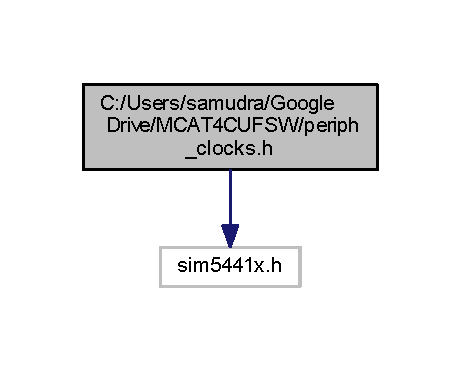
\includegraphics[width=221pt]{periph__clocks_8h__incl}
\end{center}
\end{figure}
This graph shows which files directly or indirectly include this file\+:
\nopagebreak
\begin{figure}[H]
\begin{center}
\leavevmode
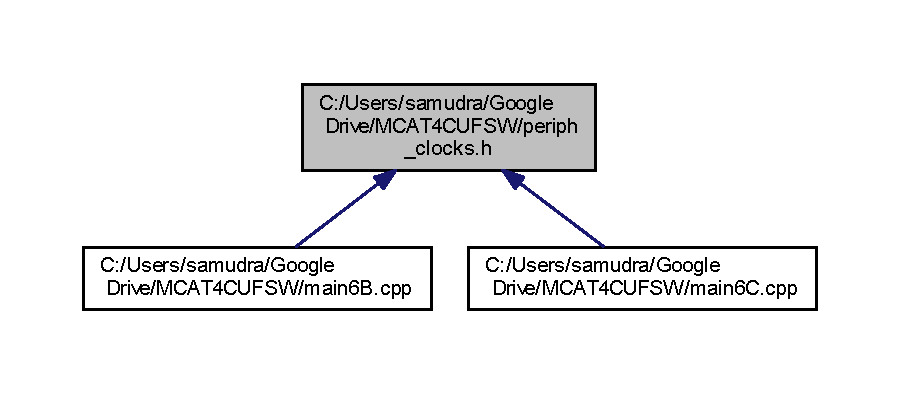
\includegraphics[width=350pt]{periph__clocks_8h__dep__incl}
\end{center}
\end{figure}
\subsection*{Macros}
\begin{DoxyCompactItemize}
\item 
\#define \hyperlink{periph__clocks_8h_a1a69d8fef468cc120a87c0053c76c242}{P\+E\+R\+I\+P\+H\+\_\+\+C\+L\+O\+C\+K\+\_\+\+F\+L\+E\+X\+B\+U\+S}~2
\item 
\#define \hyperlink{periph__clocks_8h_afbc8abb5895c39b9d2d832d8bb92c375}{P\+E\+R\+I\+P\+H\+\_\+\+C\+L\+O\+C\+K\+\_\+\+C\+A\+N\+\_\+0}~8
\item 
\#define \hyperlink{periph__clocks_8h_a4e11176742f49726726c8184f4f1282b}{P\+E\+R\+I\+P\+H\+\_\+\+C\+L\+O\+C\+K\+\_\+\+C\+A\+N\+\_\+1}~9
\item 
\#define \hyperlink{periph__clocks_8h_a9602fb01b80d39aa3b06fff96f97232a}{P\+E\+R\+I\+P\+H\+\_\+\+C\+L\+O\+C\+K\+\_\+\+I2\+C\+\_\+1}~14
\item 
\#define \hyperlink{periph__clocks_8h_ada031795b1766dbced1eb95d049e14cd}{P\+E\+R\+I\+P\+H\+\_\+\+C\+L\+O\+C\+K\+\_\+\+D\+S\+P\+I\+\_\+1}~15
\item 
\#define \hyperlink{periph__clocks_8h_a20daba47a6e7e59a21b927f50af419ca}{P\+E\+R\+I\+P\+H\+\_\+\+C\+L\+O\+C\+K\+\_\+\+D\+M\+A}~17
\item 
\#define \hyperlink{periph__clocks_8h_a31e4f6226a5420b48c75c8259a575ce7}{P\+E\+R\+I\+P\+H\+\_\+\+C\+L\+O\+C\+K\+\_\+\+I\+N\+T\+C\+\_\+0}~18
\item 
\#define \hyperlink{periph__clocks_8h_a68ab5546a409a4e2b1046d7ada445b86}{P\+E\+R\+I\+P\+H\+\_\+\+C\+L\+O\+C\+K\+\_\+\+I\+N\+T\+C\+\_\+1}~19
\item 
\#define \hyperlink{periph__clocks_8h_a1ffc185473c47f2ae7c37455ac853d4e}{P\+E\+R\+I\+P\+H\+\_\+\+C\+L\+O\+C\+K\+\_\+\+I\+N\+T\+C\+\_\+2}~20
\item 
\#define \hyperlink{periph__clocks_8h_a7f4d2838c08848162227da10e21128d2}{P\+E\+R\+I\+P\+H\+\_\+\+C\+L\+O\+C\+K\+\_\+\+I2\+C\+\_\+0}~22
\item 
\#define \hyperlink{periph__clocks_8h_a8cbaf623a61028842bd3f030ff6e6fdb}{P\+E\+R\+I\+P\+H\+\_\+\+C\+L\+O\+C\+K\+\_\+\+D\+S\+P\+I\+\_\+0}~23
\item 
\#define \hyperlink{periph__clocks_8h_a804badc7aa1241bb06a10a64d907f26c}{P\+E\+R\+I\+P\+H\+\_\+\+C\+L\+O\+C\+K\+\_\+\+U\+A\+R\+T\+\_\+0}~24
\item 
\#define \hyperlink{periph__clocks_8h_ad90f8b6026625ee5c732d14998f5a27b}{P\+E\+R\+I\+P\+H\+\_\+\+C\+L\+O\+C\+K\+\_\+\+U\+A\+R\+T\+\_\+1}~25
\item 
\#define \hyperlink{periph__clocks_8h_a26fb95398064a9d37d40d173a7df2685}{P\+E\+R\+I\+P\+H\+\_\+\+C\+L\+O\+C\+K\+\_\+\+U\+A\+R\+T\+\_\+2}~26
\item 
\#define \hyperlink{periph__clocks_8h_ad9cead62cae897839bb310f2b69eb23b}{P\+E\+R\+I\+P\+H\+\_\+\+C\+L\+O\+C\+K\+\_\+\+U\+A\+R\+T\+\_\+3}~27
\item 
\#define \hyperlink{periph__clocks_8h_af50f6235d2d192776874657f4bc73bc8}{P\+E\+R\+I\+P\+H\+\_\+\+C\+L\+O\+C\+K\+\_\+\+D\+M\+A\+\_\+\+T\+M\+R\+\_\+0}~28
\item 
\#define \hyperlink{periph__clocks_8h_a6c18aaf684c186880fba5611d77f35f3}{P\+E\+R\+I\+P\+H\+\_\+\+C\+L\+O\+C\+K\+\_\+\+D\+M\+A\+\_\+\+T\+M\+R\+\_\+1}~29
\item 
\#define \hyperlink{periph__clocks_8h_a28b9a492627a2bea49529cd7254bfe8f}{P\+E\+R\+I\+P\+H\+\_\+\+C\+L\+O\+C\+K\+\_\+\+D\+M\+A\+\_\+\+T\+M\+R\+\_\+2}~30
\item 
\#define \hyperlink{periph__clocks_8h_a7eef662631e7a9371697a776e6bb9f7c}{P\+E\+R\+I\+P\+H\+\_\+\+C\+L\+O\+C\+K\+\_\+\+D\+M\+A\+\_\+\+T\+M\+R\+\_\+3}~31
\item 
\#define \hyperlink{periph__clocks_8h_ad8401799aba7139d18f94c97d02928c7}{P\+E\+R\+I\+P\+H\+\_\+\+C\+L\+O\+C\+K\+\_\+\+P\+I\+T\+\_\+0}~32
\item 
\#define \hyperlink{periph__clocks_8h_a42f2ea017dd2a621cb69b459b19aede1}{P\+E\+R\+I\+P\+H\+\_\+\+C\+L\+O\+C\+K\+\_\+\+P\+I\+T\+\_\+1}~33
\item 
\#define \hyperlink{periph__clocks_8h_ada9881cdbd8350e583ad77a0e6d5e61a}{P\+E\+R\+I\+P\+H\+\_\+\+C\+L\+O\+C\+K\+\_\+\+P\+I\+T\+\_\+2}~34
\item 
\#define \hyperlink{periph__clocks_8h_a2891e082b3291d0831667e6ab8eba601}{P\+E\+R\+I\+P\+H\+\_\+\+C\+L\+O\+C\+K\+\_\+\+P\+I\+T\+\_\+3}~35
\item 
\#define \hyperlink{periph__clocks_8h_a96c7d44af2842b64ae863a9453630c0d}{P\+E\+R\+I\+P\+H\+\_\+\+C\+L\+O\+C\+K\+\_\+\+E\+D\+G\+E\+\_\+\+P\+O\+R\+T}~36
\item 
\#define \hyperlink{periph__clocks_8h_a455a2224b8ab740414e8ca36a19d964b}{P\+E\+R\+I\+P\+H\+\_\+\+C\+L\+O\+C\+K\+\_\+\+A\+D\+C}~37
\item 
\#define \hyperlink{periph__clocks_8h_ac5df90795a2778086fce5ee4c82d39c8}{P\+E\+R\+I\+P\+H\+\_\+\+C\+L\+O\+C\+K\+\_\+\+D\+A\+C\+\_\+0}~38
\item 
\#define \hyperlink{periph__clocks_8h_adfdd7b09ca6e055699e72102e3e1b078}{P\+E\+R\+I\+P\+H\+\_\+\+C\+L\+O\+C\+K\+\_\+\+R\+T\+C}~42
\item 
\#define \hyperlink{periph__clocks_8h_a703048470c86d41dfd012fda19006206}{P\+E\+R\+I\+P\+H\+\_\+\+C\+L\+O\+C\+K\+\_\+\+S\+I\+M}~43
\item 
\#define \hyperlink{periph__clocks_8h_a13d596ba3e62d9309cbda006dcbd0c8d}{P\+E\+R\+I\+P\+H\+\_\+\+C\+L\+O\+C\+K\+\_\+\+U\+S\+B\+\_\+\+O\+T\+G}~44
\item 
\#define \hyperlink{periph__clocks_8h_aba64b6c42b01b170621e68f17a289329}{P\+E\+R\+I\+P\+H\+\_\+\+C\+L\+O\+C\+K\+\_\+\+U\+S\+B\+\_\+\+H\+O\+S\+T}~45
\item 
\#define \hyperlink{periph__clocks_8h_a55a59146990c836fd6184f0b235e888e}{P\+E\+R\+I\+P\+H\+\_\+\+C\+L\+O\+C\+K\+\_\+\+D\+D\+R}~46
\item 
\#define \hyperlink{periph__clocks_8h_a79e536f3d7134bab4ce7018df46b9f09}{P\+E\+R\+I\+P\+H\+\_\+\+C\+L\+O\+C\+K\+\_\+\+S\+S\+I\+\_\+0}~47
\item 
\#define \hyperlink{periph__clocks_8h_abade9401df9d7831e0794fcaafa7c627}{P\+E\+R\+I\+P\+H\+\_\+\+C\+L\+O\+C\+K\+\_\+\+P\+L\+L}~48
\item 
\#define \hyperlink{periph__clocks_8h_aa7cbb5c2b68772db08ad7a1cbaeadb1f}{P\+E\+R\+I\+P\+H\+\_\+\+C\+L\+O\+C\+K\+\_\+\+R\+N\+G}~49
\item 
\#define \hyperlink{periph__clocks_8h_abc7acb3662a4b52aede9fee1cc0674c8}{P\+E\+R\+I\+P\+H\+\_\+\+C\+L\+O\+C\+K\+\_\+\+S\+S\+I\+\_\+1}~50
\item 
\#define \hyperlink{periph__clocks_8h_a2e12048f84f635a98f142c81697a314b}{P\+E\+R\+I\+P\+H\+\_\+\+C\+L\+O\+C\+K\+\_\+\+S\+D\+H\+C}~52
\item 
\#define \hyperlink{periph__clocks_8h_aa76674f8034361e947cdd76ff15e4f2d}{P\+E\+R\+I\+P\+H\+\_\+\+C\+L\+O\+C\+K\+\_\+\+M\+A\+C\+N\+E\+T\+\_\+0}~53
\item 
\#define \hyperlink{periph__clocks_8h_a89f8ec57f68ec9e5e77e79085f59c847}{P\+E\+R\+I\+P\+H\+\_\+\+C\+L\+O\+C\+K\+\_\+\+M\+A\+C\+N\+E\+T\+\_\+1}~54
\item 
\#define \hyperlink{periph__clocks_8h_a0f990b359d468a0d998e99ce5b54d519}{P\+E\+R\+I\+P\+H\+\_\+\+C\+L\+O\+C\+K\+\_\+\+E\+T\+H\+E\+R\+N\+E\+T\+\_\+\+S\+W\+I\+T\+C\+H\+\_\+0}~55
\item 
\#define \hyperlink{periph__clocks_8h_aae4dba748d63a350140d987bffe41e4e}{P\+E\+R\+I\+P\+H\+\_\+\+C\+L\+O\+C\+K\+\_\+\+E\+T\+H\+E\+R\+N\+E\+T\+\_\+\+S\+W\+I\+T\+C\+H\+\_\+1}~56
\item 
\#define \hyperlink{periph__clocks_8h_a7f76150798714f23f018198a04e549d0}{P\+E\+R\+I\+P\+H\+\_\+\+C\+L\+O\+C\+K\+\_\+\+N\+A\+N\+D\+\_\+\+F\+L\+A\+S\+H}~63
\item 
\#define \hyperlink{periph__clocks_8h_aca9135d992ac87a425ecd6967fa39dd0}{P\+E\+R\+I\+P\+H\+\_\+\+C\+L\+O\+C\+K\+\_\+\+P\+W\+M}~34
\item 
\#define \hyperlink{periph__clocks_8h_a9172e3338802269e2b8194b741a46ca5}{P\+E\+R\+I\+P\+H\+\_\+\+C\+L\+O\+C\+K\+\_\+\+C\+C\+M\+\_\+\+R\+E\+S\+E\+T}~36
\item 
\#define \hyperlink{periph__clocks_8h_af915d0fe7b8a68d94b1a90da8fc48522}{P\+E\+R\+I\+P\+H\+\_\+\+C\+L\+O\+C\+K\+\_\+\+G\+P\+I\+O}~37
\item 
\#define \hyperlink{periph__clocks_8h_aac9a82707127d19dd2d305407b5cf9ee}{P\+E\+R\+I\+P\+H\+\_\+\+C\+L\+O\+C\+K\+\_\+1\+\_\+\+W\+I\+R\+E}~2
\item 
\#define \hyperlink{periph__clocks_8h_ae1b8c97a06df9ee67717c065d930992e}{P\+E\+R\+I\+P\+H\+\_\+\+C\+L\+O\+C\+K\+\_\+\+I2\+C\+\_\+2}~4
\item 
\#define \hyperlink{periph__clocks_8h_a220edb31b451726855c5463e6ab2fbca}{P\+E\+R\+I\+P\+H\+\_\+\+C\+L\+O\+C\+K\+\_\+\+I2\+C\+\_\+3}~5
\item 
\#define \hyperlink{periph__clocks_8h_ae8fd2b4295bcd5e593dcc292f7f1afc4}{P\+E\+R\+I\+P\+H\+\_\+\+C\+L\+O\+C\+K\+\_\+\+I2\+C\+\_\+4}~6
\item 
\#define \hyperlink{periph__clocks_8h_a4ac8aac34e49868d417a9a1667169999}{P\+E\+R\+I\+P\+H\+\_\+\+C\+L\+O\+C\+K\+\_\+\+I2\+C\+\_\+5}~7
\item 
\#define \hyperlink{periph__clocks_8h_af8ff3839ca957ab87659bd6bed7e967f}{P\+E\+R\+I\+P\+H\+\_\+\+C\+L\+O\+C\+K\+\_\+\+D\+S\+P\+I\+\_\+2}~14
\item 
\#define \hyperlink{periph__clocks_8h_abd8503047d052fe12492764f4a658f17}{P\+E\+R\+I\+P\+H\+\_\+\+C\+L\+O\+C\+K\+\_\+\+D\+S\+P\+I\+\_\+3}~15
\item 
\#define \hyperlink{periph__clocks_8h_a50f2965940b8347df7919295c6506034}{P\+E\+R\+I\+P\+H\+\_\+\+C\+L\+O\+C\+K\+\_\+\+U\+A\+R\+T\+\_\+4}~24
\item 
\#define \hyperlink{periph__clocks_8h_ad70966231218a8d712b5a3eccb58b1a2}{P\+E\+R\+I\+P\+H\+\_\+\+C\+L\+O\+C\+K\+\_\+\+U\+A\+R\+T\+\_\+5}~25
\item 
\#define \hyperlink{periph__clocks_8h_ab396c628c4428866091536c8a51e8cee}{P\+E\+R\+I\+P\+H\+\_\+\+C\+L\+O\+C\+K\+\_\+\+U\+A\+R\+T\+\_\+6}~26
\item 
\#define \hyperlink{periph__clocks_8h_afc544d82aacae0cca5dab7692cf47fb3}{P\+E\+R\+I\+P\+H\+\_\+\+C\+L\+O\+C\+K\+\_\+\+U\+A\+R\+T\+\_\+7}~27
\item 
\#define \hyperlink{periph__clocks_8h_a83f559dfb9eddec1dc297734fa03d2e5}{P\+E\+R\+I\+P\+H\+\_\+\+C\+L\+O\+C\+K\+\_\+\+U\+A\+R\+T\+\_\+8}~28
\item 
\#define \hyperlink{periph__clocks_8h_adf54ba14b371f1bf7a562451b3da38a4}{P\+E\+R\+I\+P\+H\+\_\+\+C\+L\+O\+C\+K\+\_\+\+U\+A\+R\+T\+\_\+9}~29
\item 
\#define \hyperlink{periph__clocks_8h_a43d8ed8e42ed5b183aae89e7867f013e}{P\+E\+R\+I\+P\+H\+\_\+\+D\+I\+S\+A\+B\+L\+E\+\_\+\+F\+L\+E\+X\+B\+U\+S}~sim2.\+scm.\+ppmsr0 = \hyperlink{periph__clocks_8h_a1a69d8fef468cc120a87c0053c76c242}{P\+E\+R\+I\+P\+H\+\_\+\+C\+L\+O\+C\+K\+\_\+\+F\+L\+E\+X\+B\+U\+S}
\item 
\#define \hyperlink{periph__clocks_8h_a5391a00bbd257b7463d3484a2fb93f01}{P\+E\+R\+I\+P\+H\+\_\+\+D\+I\+S\+A\+B\+L\+E\+\_\+\+C\+A\+N\+\_\+0}~sim2.\+scm.\+ppmsr0 = \hyperlink{periph__clocks_8h_afbc8abb5895c39b9d2d832d8bb92c375}{P\+E\+R\+I\+P\+H\+\_\+\+C\+L\+O\+C\+K\+\_\+\+C\+A\+N\+\_\+0}
\item 
\#define \hyperlink{periph__clocks_8h_ae522b74f538efc9d6af455eceb016fc2}{P\+E\+R\+I\+P\+H\+\_\+\+D\+I\+S\+A\+B\+L\+E\+\_\+\+C\+A\+N\+\_\+1}~sim2.\+scm.\+ppmsr0 = \hyperlink{periph__clocks_8h_a4e11176742f49726726c8184f4f1282b}{P\+E\+R\+I\+P\+H\+\_\+\+C\+L\+O\+C\+K\+\_\+\+C\+A\+N\+\_\+1}
\item 
\#define \hyperlink{periph__clocks_8h_a9ab1f81c5993d1164f4fe139846b05cf}{P\+E\+R\+I\+P\+H\+\_\+\+D\+I\+S\+A\+B\+L\+E\+\_\+\+I2\+C\+\_\+1}~sim2.\+scm.\+ppmsr0 = \hyperlink{periph__clocks_8h_a9602fb01b80d39aa3b06fff96f97232a}{P\+E\+R\+I\+P\+H\+\_\+\+C\+L\+O\+C\+K\+\_\+\+I2\+C\+\_\+1}
\item 
\#define \hyperlink{periph__clocks_8h_a737eaab06b116f705d8e74125d87ea45}{P\+E\+R\+I\+P\+H\+\_\+\+D\+I\+S\+A\+B\+L\+E\+\_\+\+D\+S\+P\+I\+\_\+1}~sim2.\+scm.\+ppmsr0 = \hyperlink{periph__clocks_8h_ada031795b1766dbced1eb95d049e14cd}{P\+E\+R\+I\+P\+H\+\_\+\+C\+L\+O\+C\+K\+\_\+\+D\+S\+P\+I\+\_\+1}
\item 
\#define \hyperlink{periph__clocks_8h_a82902b3449cfedf91e37e8f4efe1763d}{P\+E\+R\+I\+P\+H\+\_\+\+D\+I\+S\+A\+B\+L\+E\+\_\+\+D\+M\+A}~sim2.\+scm.\+ppmsr0 = \hyperlink{periph__clocks_8h_a20daba47a6e7e59a21b927f50af419ca}{P\+E\+R\+I\+P\+H\+\_\+\+C\+L\+O\+C\+K\+\_\+\+D\+M\+A}
\item 
\#define \hyperlink{periph__clocks_8h_a7e917f13e34becb0a1a9480e3bbe764f}{P\+E\+R\+I\+P\+H\+\_\+\+D\+I\+S\+A\+B\+L\+E\+\_\+\+I\+N\+T\+C\+\_\+0}~sim2.\+scm.\+ppmsr0 = \hyperlink{periph__clocks_8h_a31e4f6226a5420b48c75c8259a575ce7}{P\+E\+R\+I\+P\+H\+\_\+\+C\+L\+O\+C\+K\+\_\+\+I\+N\+T\+C\+\_\+0}
\item 
\#define \hyperlink{periph__clocks_8h_aca9bddcda52622a9ef485942291b2ac9}{P\+E\+R\+I\+P\+H\+\_\+\+D\+I\+S\+A\+B\+L\+E\+\_\+\+I\+N\+T\+C\+\_\+1}~sim2.\+scm.\+ppmsr0 = \hyperlink{periph__clocks_8h_a68ab5546a409a4e2b1046d7ada445b86}{P\+E\+R\+I\+P\+H\+\_\+\+C\+L\+O\+C\+K\+\_\+\+I\+N\+T\+C\+\_\+1}
\item 
\#define \hyperlink{periph__clocks_8h_a33e5180046f6e098d56b8b1a7216a816}{P\+E\+R\+I\+P\+H\+\_\+\+D\+I\+S\+A\+B\+L\+E\+\_\+\+I\+N\+T\+C\+\_\+2}~sim2.\+scm.\+ppmsr0 = \hyperlink{periph__clocks_8h_a1ffc185473c47f2ae7c37455ac853d4e}{P\+E\+R\+I\+P\+H\+\_\+\+C\+L\+O\+C\+K\+\_\+\+I\+N\+T\+C\+\_\+2}
\item 
\#define \hyperlink{periph__clocks_8h_ade22f2f50fd41364161faae93e113bba}{P\+E\+R\+I\+P\+H\+\_\+\+D\+I\+S\+A\+B\+L\+E\+\_\+\+I2\+C\+\_\+0}~sim2.\+scm.\+ppmsr0 = \hyperlink{periph__clocks_8h_a7f4d2838c08848162227da10e21128d2}{P\+E\+R\+I\+P\+H\+\_\+\+C\+L\+O\+C\+K\+\_\+\+I2\+C\+\_\+0}
\item 
\#define \hyperlink{periph__clocks_8h_a1be94c629299a70c08d4c9f333e9164e}{P\+E\+R\+I\+P\+H\+\_\+\+D\+I\+S\+A\+B\+L\+E\+\_\+\+D\+S\+P\+I\+\_\+0}~sim2.\+scm.\+ppmsr0 = \hyperlink{periph__clocks_8h_a8cbaf623a61028842bd3f030ff6e6fdb}{P\+E\+R\+I\+P\+H\+\_\+\+C\+L\+O\+C\+K\+\_\+\+D\+S\+P\+I\+\_\+0}
\item 
\#define \hyperlink{periph__clocks_8h_aea6fc6bc46c976716cde8af44ff3cecd}{P\+E\+R\+I\+P\+H\+\_\+\+D\+I\+S\+A\+B\+L\+E\+\_\+\+U\+A\+R\+T\+\_\+0}~sim2.\+scm.\+ppmsr0 = \hyperlink{periph__clocks_8h_a804badc7aa1241bb06a10a64d907f26c}{P\+E\+R\+I\+P\+H\+\_\+\+C\+L\+O\+C\+K\+\_\+\+U\+A\+R\+T\+\_\+0}
\item 
\#define \hyperlink{periph__clocks_8h_ad8177d1aa7d76e1806ad2a5c489e81b8}{P\+E\+R\+I\+P\+H\+\_\+\+D\+I\+S\+A\+B\+L\+E\+\_\+\+U\+A\+R\+T\+\_\+1}~sim2.\+scm.\+ppmsr0 = \hyperlink{periph__clocks_8h_ad90f8b6026625ee5c732d14998f5a27b}{P\+E\+R\+I\+P\+H\+\_\+\+C\+L\+O\+C\+K\+\_\+\+U\+A\+R\+T\+\_\+1}
\item 
\#define \hyperlink{periph__clocks_8h_a195e1d78107d52cb56641be54ff2d5c1}{P\+E\+R\+I\+P\+H\+\_\+\+D\+I\+S\+A\+B\+L\+E\+\_\+\+U\+A\+R\+T\+\_\+2}~sim2.\+scm.\+ppmsr0 = \hyperlink{periph__clocks_8h_a26fb95398064a9d37d40d173a7df2685}{P\+E\+R\+I\+P\+H\+\_\+\+C\+L\+O\+C\+K\+\_\+\+U\+A\+R\+T\+\_\+2}
\item 
\#define \hyperlink{periph__clocks_8h_a7b63448bc23a9fe0529c16bc71a32fb2}{P\+E\+R\+I\+P\+H\+\_\+\+D\+I\+S\+A\+B\+L\+E\+\_\+\+U\+A\+R\+T\+\_\+3}~sim2.\+scm.\+ppmsr0 = \hyperlink{periph__clocks_8h_ad9cead62cae897839bb310f2b69eb23b}{P\+E\+R\+I\+P\+H\+\_\+\+C\+L\+O\+C\+K\+\_\+\+U\+A\+R\+T\+\_\+3}
\item 
\#define \hyperlink{periph__clocks_8h_ae4406850f08137d45a1d0f836fac35a1}{P\+E\+R\+I\+P\+H\+\_\+\+D\+I\+S\+A\+B\+L\+E\+\_\+\+D\+M\+A\+\_\+\+T\+M\+R\+\_\+0}~sim2.\+scm.\+ppmsr0 = \hyperlink{periph__clocks_8h_af50f6235d2d192776874657f4bc73bc8}{P\+E\+R\+I\+P\+H\+\_\+\+C\+L\+O\+C\+K\+\_\+\+D\+M\+A\+\_\+\+T\+M\+R\+\_\+0}
\item 
\#define \hyperlink{periph__clocks_8h_a151351b872dfae37b1a4ed694e4bde0f}{P\+E\+R\+I\+P\+H\+\_\+\+D\+I\+S\+A\+B\+L\+E\+\_\+\+D\+M\+A\+\_\+\+T\+M\+R\+\_\+1}~sim2.\+scm.\+ppmsr0 = \hyperlink{periph__clocks_8h_a6c18aaf684c186880fba5611d77f35f3}{P\+E\+R\+I\+P\+H\+\_\+\+C\+L\+O\+C\+K\+\_\+\+D\+M\+A\+\_\+\+T\+M\+R\+\_\+1}
\item 
\#define \hyperlink{periph__clocks_8h_aed1a81dc2347c3a8fce24a3501c2ada0}{P\+E\+R\+I\+P\+H\+\_\+\+D\+I\+S\+A\+B\+L\+E\+\_\+\+D\+M\+A\+\_\+\+T\+M\+R\+\_\+2}~sim2.\+scm.\+ppmsr0 = \hyperlink{periph__clocks_8h_a28b9a492627a2bea49529cd7254bfe8f}{P\+E\+R\+I\+P\+H\+\_\+\+C\+L\+O\+C\+K\+\_\+\+D\+M\+A\+\_\+\+T\+M\+R\+\_\+2}
\item 
\#define \hyperlink{periph__clocks_8h_abce92c0e5bc2ebe7774c9874bbdaf18e}{P\+E\+R\+I\+P\+H\+\_\+\+E\+N\+A\+B\+L\+E\+\_\+\+F\+L\+E\+X\+B\+U\+S}~sim2.\+scm.\+ppmcr0 = \hyperlink{periph__clocks_8h_a1a69d8fef468cc120a87c0053c76c242}{P\+E\+R\+I\+P\+H\+\_\+\+C\+L\+O\+C\+K\+\_\+\+F\+L\+E\+X\+B\+U\+S}
\item 
\#define \hyperlink{periph__clocks_8h_aa5112d00c86469c3699534b629af7e84}{P\+E\+R\+I\+P\+H\+\_\+\+E\+N\+A\+B\+L\+E\+\_\+\+C\+A\+N\+\_\+0}~sim2.\+scm.\+ppmcr0 = \hyperlink{periph__clocks_8h_afbc8abb5895c39b9d2d832d8bb92c375}{P\+E\+R\+I\+P\+H\+\_\+\+C\+L\+O\+C\+K\+\_\+\+C\+A\+N\+\_\+0}
\item 
\#define \hyperlink{periph__clocks_8h_a7de952826bd1503bc8cd06c7385464e3}{P\+E\+R\+I\+P\+H\+\_\+\+E\+N\+A\+B\+L\+E\+\_\+\+C\+A\+N\+\_\+1}~sim2.\+scm.\+ppmcr0 = \hyperlink{periph__clocks_8h_a4e11176742f49726726c8184f4f1282b}{P\+E\+R\+I\+P\+H\+\_\+\+C\+L\+O\+C\+K\+\_\+\+C\+A\+N\+\_\+1}
\item 
\#define \hyperlink{periph__clocks_8h_a35fab3ae562ec6f090c4642c04ef0702}{P\+E\+R\+I\+P\+H\+\_\+\+E\+N\+A\+B\+L\+E\+\_\+\+I2\+C\+\_\+1}~sim2.\+scm.\+ppmcr0 = \hyperlink{periph__clocks_8h_a9602fb01b80d39aa3b06fff96f97232a}{P\+E\+R\+I\+P\+H\+\_\+\+C\+L\+O\+C\+K\+\_\+\+I2\+C\+\_\+1}
\item 
\#define \hyperlink{periph__clocks_8h_a36aa676dcf790b0bcbb59400d5278ae9}{P\+E\+R\+I\+P\+H\+\_\+\+E\+N\+A\+B\+L\+E\+\_\+\+D\+S\+P\+I\+\_\+1}~sim2.\+scm.\+ppmcr0 = \hyperlink{periph__clocks_8h_ada031795b1766dbced1eb95d049e14cd}{P\+E\+R\+I\+P\+H\+\_\+\+C\+L\+O\+C\+K\+\_\+\+D\+S\+P\+I\+\_\+1}
\item 
\#define \hyperlink{periph__clocks_8h_ad33a516f1fc76d30ba2c111adc46b3e5}{P\+E\+R\+I\+P\+H\+\_\+\+E\+N\+A\+B\+L\+E\+\_\+\+D\+M\+A}~sim2.\+scm.\+ppmcr0 = \hyperlink{periph__clocks_8h_a20daba47a6e7e59a21b927f50af419ca}{P\+E\+R\+I\+P\+H\+\_\+\+C\+L\+O\+C\+K\+\_\+\+D\+M\+A}
\item 
\#define \hyperlink{periph__clocks_8h_ae7d5b5197c213767f78d1f75a80ffafc}{P\+E\+R\+I\+P\+H\+\_\+\+E\+N\+A\+B\+L\+E\+\_\+\+I\+N\+T\+C\+\_\+0}~sim2.\+scm.\+ppmcr0 = \hyperlink{periph__clocks_8h_a31e4f6226a5420b48c75c8259a575ce7}{P\+E\+R\+I\+P\+H\+\_\+\+C\+L\+O\+C\+K\+\_\+\+I\+N\+T\+C\+\_\+0}
\item 
\#define \hyperlink{periph__clocks_8h_a5edb78c0a5846853bc50c6dd175d6208}{P\+E\+R\+I\+P\+H\+\_\+\+E\+N\+A\+B\+L\+E\+\_\+\+I\+N\+T\+C\+\_\+1}~sim2.\+scm.\+ppmcr0 = \hyperlink{periph__clocks_8h_a68ab5546a409a4e2b1046d7ada445b86}{P\+E\+R\+I\+P\+H\+\_\+\+C\+L\+O\+C\+K\+\_\+\+I\+N\+T\+C\+\_\+1}
\item 
\#define \hyperlink{periph__clocks_8h_ac118476936fc3659fc93e360f27acfee}{P\+E\+R\+I\+P\+H\+\_\+\+E\+N\+A\+B\+L\+E\+\_\+\+I\+N\+T\+C\+\_\+2}~sim2.\+scm.\+ppmcr0 = \hyperlink{periph__clocks_8h_a1ffc185473c47f2ae7c37455ac853d4e}{P\+E\+R\+I\+P\+H\+\_\+\+C\+L\+O\+C\+K\+\_\+\+I\+N\+T\+C\+\_\+2}
\item 
\#define \hyperlink{periph__clocks_8h_a3dcb0ebc9f41ea992f7b14ee0a341cea}{P\+E\+R\+I\+P\+H\+\_\+\+E\+N\+A\+B\+L\+E\+\_\+\+I2\+C\+\_\+0}~sim2.\+scm.\+ppmcr0 = \hyperlink{periph__clocks_8h_a7f4d2838c08848162227da10e21128d2}{P\+E\+R\+I\+P\+H\+\_\+\+C\+L\+O\+C\+K\+\_\+\+I2\+C\+\_\+0}
\item 
\#define \hyperlink{periph__clocks_8h_a14491706a0e47d62341f18dea765e5fb}{P\+E\+R\+I\+P\+H\+\_\+\+E\+N\+A\+B\+L\+E\+\_\+\+D\+S\+P\+I\+\_\+0}~sim2.\+scm.\+ppmcr0 = \hyperlink{periph__clocks_8h_a8cbaf623a61028842bd3f030ff6e6fdb}{P\+E\+R\+I\+P\+H\+\_\+\+C\+L\+O\+C\+K\+\_\+\+D\+S\+P\+I\+\_\+0}
\item 
\#define \hyperlink{periph__clocks_8h_a40dc3b6b4d7be5e3d402872f89b7e86f}{P\+E\+R\+I\+P\+H\+\_\+\+E\+N\+A\+B\+L\+E\+\_\+\+U\+A\+R\+T\+\_\+0}~sim2.\+scm.\+ppmcr0 = \hyperlink{periph__clocks_8h_a804badc7aa1241bb06a10a64d907f26c}{P\+E\+R\+I\+P\+H\+\_\+\+C\+L\+O\+C\+K\+\_\+\+U\+A\+R\+T\+\_\+0}
\item 
\#define \hyperlink{periph__clocks_8h_a1eae78dcd6868fd9ddb237190ed68439}{P\+E\+R\+I\+P\+H\+\_\+\+E\+N\+A\+B\+L\+E\+\_\+\+U\+A\+R\+T\+\_\+1}~sim2.\+scm.\+ppmcr0 = \hyperlink{periph__clocks_8h_ad90f8b6026625ee5c732d14998f5a27b}{P\+E\+R\+I\+P\+H\+\_\+\+C\+L\+O\+C\+K\+\_\+\+U\+A\+R\+T\+\_\+1}
\item 
\#define \hyperlink{periph__clocks_8h_acd092b100985ea3b98a5df696257b99f}{P\+E\+R\+I\+P\+H\+\_\+\+E\+N\+A\+B\+L\+E\+\_\+\+U\+A\+R\+T\+\_\+2}~sim2.\+scm.\+ppmcr0 = \hyperlink{periph__clocks_8h_a26fb95398064a9d37d40d173a7df2685}{P\+E\+R\+I\+P\+H\+\_\+\+C\+L\+O\+C\+K\+\_\+\+U\+A\+R\+T\+\_\+2}
\item 
\#define \hyperlink{periph__clocks_8h_a910299b8e529b41cb7e0cf03634c2a3b}{P\+E\+R\+I\+P\+H\+\_\+\+E\+N\+A\+B\+L\+E\+\_\+\+U\+A\+R\+T\+\_\+3}~sim2.\+scm.\+ppmcr0 = \hyperlink{periph__clocks_8h_ad9cead62cae897839bb310f2b69eb23b}{P\+E\+R\+I\+P\+H\+\_\+\+C\+L\+O\+C\+K\+\_\+\+U\+A\+R\+T\+\_\+3}
\item 
\#define \hyperlink{periph__clocks_8h_af796ef0555bc5c3a1fcce0ffc2af49c3}{P\+E\+R\+I\+P\+H\+\_\+\+E\+N\+A\+B\+L\+E\+\_\+\+D\+M\+A\+\_\+\+T\+M\+R\+\_\+0}~sim2.\+scm.\+ppmcr0 = \hyperlink{periph__clocks_8h_af50f6235d2d192776874657f4bc73bc8}{P\+E\+R\+I\+P\+H\+\_\+\+C\+L\+O\+C\+K\+\_\+\+D\+M\+A\+\_\+\+T\+M\+R\+\_\+0}
\item 
\#define \hyperlink{periph__clocks_8h_a20194195f862cbd3fc9bbd7f604d7f02}{P\+E\+R\+I\+P\+H\+\_\+\+E\+N\+A\+B\+L\+E\+\_\+\+D\+M\+A\+\_\+\+T\+M\+R\+\_\+1}~sim2.\+scm.\+ppmcr0 = \hyperlink{periph__clocks_8h_a6c18aaf684c186880fba5611d77f35f3}{P\+E\+R\+I\+P\+H\+\_\+\+C\+L\+O\+C\+K\+\_\+\+D\+M\+A\+\_\+\+T\+M\+R\+\_\+1}
\item 
\#define \hyperlink{periph__clocks_8h_a0f249a164f1719ee6caee41cc8813bdf}{P\+E\+R\+I\+P\+H\+\_\+\+E\+N\+A\+B\+L\+E\+\_\+\+D\+M\+A\+\_\+\+T\+M\+R\+\_\+2}~sim2.\+scm.\+ppmcr0 = \hyperlink{periph__clocks_8h_a28b9a492627a2bea49529cd7254bfe8f}{P\+E\+R\+I\+P\+H\+\_\+\+C\+L\+O\+C\+K\+\_\+\+D\+M\+A\+\_\+\+T\+M\+R\+\_\+2}
\item 
\#define \hyperlink{periph__clocks_8h_ada9a073c17399de761b1e9acf88dd2fa}{P\+E\+R\+I\+P\+H\+\_\+\+D\+I\+S\+A\+B\+L\+E\+\_\+\+P\+I\+T\+\_\+0}~sim2.\+scm.\+ppmsr0 = \hyperlink{periph__clocks_8h_ad8401799aba7139d18f94c97d02928c7}{P\+E\+R\+I\+P\+H\+\_\+\+C\+L\+O\+C\+K\+\_\+\+P\+I\+T\+\_\+0}
\item 
\#define \hyperlink{periph__clocks_8h_a97a420e62ef512433ef59b151ce59ac6}{P\+E\+R\+I\+P\+H\+\_\+\+D\+I\+S\+A\+B\+L\+E\+\_\+\+P\+I\+T\+\_\+1}~sim2.\+scm.\+ppmsr0 = \hyperlink{periph__clocks_8h_a42f2ea017dd2a621cb69b459b19aede1}{P\+E\+R\+I\+P\+H\+\_\+\+C\+L\+O\+C\+K\+\_\+\+P\+I\+T\+\_\+1}
\item 
\#define \hyperlink{periph__clocks_8h_a8847bb0eb3788014565d82e21f75ccca}{P\+E\+R\+I\+P\+H\+\_\+\+D\+I\+S\+A\+B\+L\+E\+\_\+\+P\+I\+T\+\_\+2}~sim2.\+scm.\+ppmsr0 = \hyperlink{periph__clocks_8h_ada9881cdbd8350e583ad77a0e6d5e61a}{P\+E\+R\+I\+P\+H\+\_\+\+C\+L\+O\+C\+K\+\_\+\+P\+I\+T\+\_\+2}
\item 
\#define \hyperlink{periph__clocks_8h_a67b0d6d068216f66179b3c1e50faddb0}{P\+E\+R\+I\+P\+H\+\_\+\+D\+I\+S\+A\+B\+L\+E\+\_\+\+P\+I\+T\+\_\+3}~sim2.\+scm.\+ppmsr0 = \hyperlink{periph__clocks_8h_a2891e082b3291d0831667e6ab8eba601}{P\+E\+R\+I\+P\+H\+\_\+\+C\+L\+O\+C\+K\+\_\+\+P\+I\+T\+\_\+3}
\item 
\#define \hyperlink{periph__clocks_8h_af8511e7a94ba2d13c5aaad3f7bc125fc}{P\+E\+R\+I\+P\+H\+\_\+\+D\+I\+S\+A\+B\+L\+E\+\_\+\+E\+D\+G\+E\+\_\+\+P\+O\+R\+T}~sim2.\+scm.\+ppmsr0 = \hyperlink{periph__clocks_8h_a96c7d44af2842b64ae863a9453630c0d}{P\+E\+R\+I\+P\+H\+\_\+\+C\+L\+O\+C\+K\+\_\+\+E\+D\+G\+E\+\_\+\+P\+O\+R\+T}
\item 
\#define \hyperlink{periph__clocks_8h_ab0b7332c66652875998d3186879a541d}{P\+E\+R\+I\+P\+H\+\_\+\+D\+I\+S\+A\+B\+L\+E\+\_\+\+A\+D\+C}~sim2.\+scm.\+ppmsr0 = \hyperlink{periph__clocks_8h_a455a2224b8ab740414e8ca36a19d964b}{P\+E\+R\+I\+P\+H\+\_\+\+C\+L\+O\+C\+K\+\_\+\+A\+D\+C}
\item 
\#define \hyperlink{periph__clocks_8h_aebf8f15a56920723ac325e07ffa2d224}{P\+E\+R\+I\+P\+H\+\_\+\+D\+I\+S\+A\+B\+L\+E\+\_\+\+D\+A\+C\+\_\+0}~sim2.\+scm.\+ppmsr0 = \hyperlink{periph__clocks_8h_ac5df90795a2778086fce5ee4c82d39c8}{P\+E\+R\+I\+P\+H\+\_\+\+C\+L\+O\+C\+K\+\_\+\+D\+A\+C\+\_\+0}
\item 
\#define \hyperlink{periph__clocks_8h_a439a2f074750732c48485c7f9ca61047}{P\+E\+R\+I\+P\+H\+\_\+\+D\+I\+S\+A\+B\+L\+E\+\_\+\+R\+T\+C}~sim2.\+scm.\+ppmsr0 = \hyperlink{periph__clocks_8h_adfdd7b09ca6e055699e72102e3e1b078}{P\+E\+R\+I\+P\+H\+\_\+\+C\+L\+O\+C\+K\+\_\+\+R\+T\+C}
\item 
\#define \hyperlink{periph__clocks_8h_a5f4f587f5015f07cc990d2298bb145c8}{P\+E\+R\+I\+P\+H\+\_\+\+D\+I\+S\+A\+B\+L\+E\+\_\+\+S\+I\+M}~sim2.\+scm.\+ppmsr0 = \hyperlink{periph__clocks_8h_a703048470c86d41dfd012fda19006206}{P\+E\+R\+I\+P\+H\+\_\+\+C\+L\+O\+C\+K\+\_\+\+S\+I\+M}
\item 
\#define \hyperlink{periph__clocks_8h_a4530a4dd23a0660d0b0a614198def413}{P\+E\+R\+I\+P\+H\+\_\+\+D\+I\+S\+A\+B\+L\+E\+\_\+\+U\+S\+B\+\_\+\+O\+T\+G}~sim2.\+scm.\+ppmsr0 = \hyperlink{periph__clocks_8h_a13d596ba3e62d9309cbda006dcbd0c8d}{P\+E\+R\+I\+P\+H\+\_\+\+C\+L\+O\+C\+K\+\_\+\+U\+S\+B\+\_\+\+O\+T\+G}
\item 
\#define \hyperlink{periph__clocks_8h_a891460ef84802faee6dcca9bef92f85a}{P\+E\+R\+I\+P\+H\+\_\+\+D\+I\+S\+A\+B\+L\+E\+\_\+\+U\+S\+B\+\_\+\+H\+O\+S\+T}~sim2.\+scm.\+ppmsr0 = \hyperlink{periph__clocks_8h_aba64b6c42b01b170621e68f17a289329}{P\+E\+R\+I\+P\+H\+\_\+\+C\+L\+O\+C\+K\+\_\+\+U\+S\+B\+\_\+\+H\+O\+S\+T}
\item 
\#define \hyperlink{periph__clocks_8h_a20add69212de2813ac307ecb0c057ca6}{P\+E\+R\+I\+P\+H\+\_\+\+D\+I\+S\+A\+B\+L\+E\+\_\+\+D\+D\+R}~sim2.\+scm.\+ppmsr0 = \hyperlink{periph__clocks_8h_a55a59146990c836fd6184f0b235e888e}{P\+E\+R\+I\+P\+H\+\_\+\+C\+L\+O\+C\+K\+\_\+\+D\+D\+R}
\item 
\#define \hyperlink{periph__clocks_8h_a7768b26b40f6f846d4c8699d73a848cc}{P\+E\+R\+I\+P\+H\+\_\+\+D\+I\+S\+A\+B\+L\+E\+\_\+\+S\+S\+I\+\_\+0}~sim2.\+scm.\+ppmsr0 = \hyperlink{periph__clocks_8h_a79e536f3d7134bab4ce7018df46b9f09}{P\+E\+R\+I\+P\+H\+\_\+\+C\+L\+O\+C\+K\+\_\+\+S\+S\+I\+\_\+0}
\item 
\#define \hyperlink{periph__clocks_8h_ae836af256ffb833afc207e84a01333b6}{P\+E\+R\+I\+P\+H\+\_\+\+D\+I\+S\+A\+B\+L\+E\+\_\+\+P\+L\+L}~sim2.\+scm.\+ppmsr0 = \hyperlink{periph__clocks_8h_abade9401df9d7831e0794fcaafa7c627}{P\+E\+R\+I\+P\+H\+\_\+\+C\+L\+O\+C\+K\+\_\+\+P\+L\+L}
\item 
\#define \hyperlink{periph__clocks_8h_a5118de4a2656ad0bed4c4ac11bc12918}{P\+E\+R\+I\+P\+H\+\_\+\+D\+I\+S\+A\+B\+L\+E\+\_\+\+R\+N\+G}~sim2.\+scm.\+ppmsr0 = \hyperlink{periph__clocks_8h_aa7cbb5c2b68772db08ad7a1cbaeadb1f}{P\+E\+R\+I\+P\+H\+\_\+\+C\+L\+O\+C\+K\+\_\+\+R\+N\+G}
\item 
\#define \hyperlink{periph__clocks_8h_afebad4e32791fb1a05c5ad970307f572}{P\+E\+R\+I\+P\+H\+\_\+\+D\+I\+S\+A\+B\+L\+E\+\_\+\+S\+S\+I\+\_\+1}~sim2.\+scm.\+ppmsr0 = \hyperlink{periph__clocks_8h_abc7acb3662a4b52aede9fee1cc0674c8}{P\+E\+R\+I\+P\+H\+\_\+\+C\+L\+O\+C\+K\+\_\+\+S\+S\+I\+\_\+1}
\item 
\#define \hyperlink{periph__clocks_8h_a2d591b7fc9fdecf96a7b23afdfd6dd22}{P\+E\+R\+I\+P\+H\+\_\+\+D\+I\+S\+A\+B\+L\+E\+\_\+\+S\+D\+H\+C}~sim2.\+scm.\+ppmsr0 = \hyperlink{periph__clocks_8h_a2e12048f84f635a98f142c81697a314b}{P\+E\+R\+I\+P\+H\+\_\+\+C\+L\+O\+C\+K\+\_\+\+S\+D\+H\+C}
\item 
\#define \hyperlink{periph__clocks_8h_a7fe510c04e954386088c95d29696fa2c}{P\+E\+R\+I\+P\+H\+\_\+\+D\+I\+S\+A\+B\+L\+E\+\_\+\+M\+A\+C\+N\+E\+T\+\_\+0}~sim2.\+scm.\+ppmsr0 = \hyperlink{periph__clocks_8h_aa76674f8034361e947cdd76ff15e4f2d}{P\+E\+R\+I\+P\+H\+\_\+\+C\+L\+O\+C\+K\+\_\+\+M\+A\+C\+N\+E\+T\+\_\+0}
\item 
\#define \hyperlink{periph__clocks_8h_ae28dedac5544d36c941be2b0b0652992}{P\+E\+R\+I\+P\+H\+\_\+\+D\+I\+S\+A\+B\+L\+E\+\_\+\+M\+A\+C\+N\+E\+T\+\_\+1}~sim2.\+scm.\+ppmsr0 = \hyperlink{periph__clocks_8h_a89f8ec57f68ec9e5e77e79085f59c847}{P\+E\+R\+I\+P\+H\+\_\+\+C\+L\+O\+C\+K\+\_\+\+M\+A\+C\+N\+E\+T\+\_\+1}
\item 
\#define \hyperlink{periph__clocks_8h_ac057f4830b0894d15efe5370037a657d}{P\+E\+R\+I\+P\+H\+\_\+\+D\+I\+S\+A\+B\+L\+E\+\_\+\+E\+T\+H\+E\+R\+N\+E\+T\+\_\+\+S\+W\+I\+T\+C\+H\+\_\+0}~sim2.\+scm.\+ppmsr0 = \hyperlink{periph__clocks_8h_a0f990b359d468a0d998e99ce5b54d519}{P\+E\+R\+I\+P\+H\+\_\+\+C\+L\+O\+C\+K\+\_\+\+E\+T\+H\+E\+R\+N\+E\+T\+\_\+\+S\+W\+I\+T\+C\+H\+\_\+0}
\item 
\#define \hyperlink{periph__clocks_8h_a403254a7a92488d4f5634e446bf30e50}{P\+E\+R\+I\+P\+H\+\_\+\+D\+I\+S\+A\+B\+L\+E\+\_\+\+E\+T\+H\+E\+R\+N\+E\+T\+\_\+\+S\+W\+I\+T\+C\+H\+\_\+1}~sim2.\+scm.\+ppmsr0 = \hyperlink{periph__clocks_8h_aae4dba748d63a350140d987bffe41e4e}{P\+E\+R\+I\+P\+H\+\_\+\+C\+L\+O\+C\+K\+\_\+\+E\+T\+H\+E\+R\+N\+E\+T\+\_\+\+S\+W\+I\+T\+C\+H\+\_\+1}
\item 
\#define \hyperlink{periph__clocks_8h_a6ba5589f5838afd912a58fd339d04a1d}{P\+E\+R\+I\+P\+H\+\_\+\+D\+I\+S\+A\+B\+L\+E\+\_\+\+N\+A\+N\+D\+\_\+\+F\+L\+A\+S\+H}~sim2.\+scm.\+ppmsr0 = \hyperlink{periph__clocks_8h_a7f76150798714f23f018198a04e549d0}{P\+E\+R\+I\+P\+H\+\_\+\+C\+L\+O\+C\+K\+\_\+\+N\+A\+N\+D\+\_\+\+F\+L\+A\+S\+H}
\item 
\#define \hyperlink{periph__clocks_8h_af476b8e1fc03d95fb97c3d1adb940694}{P\+E\+R\+I\+P\+H\+\_\+\+E\+N\+A\+B\+L\+E\+\_\+\+P\+I\+T\+\_\+0}~sim2.\+scm.\+ppmcr0 = \hyperlink{periph__clocks_8h_ad8401799aba7139d18f94c97d02928c7}{P\+E\+R\+I\+P\+H\+\_\+\+C\+L\+O\+C\+K\+\_\+\+P\+I\+T\+\_\+0}
\item 
\#define \hyperlink{periph__clocks_8h_aaa24f4628623c34c6fa0d19bc906430a}{P\+E\+R\+I\+P\+H\+\_\+\+E\+N\+A\+B\+L\+E\+\_\+\+P\+I\+T\+\_\+1}~sim2.\+scm.\+ppmcr0 = \hyperlink{periph__clocks_8h_a42f2ea017dd2a621cb69b459b19aede1}{P\+E\+R\+I\+P\+H\+\_\+\+C\+L\+O\+C\+K\+\_\+\+P\+I\+T\+\_\+1}
\item 
\#define \hyperlink{periph__clocks_8h_a1555993a496011ca17a2def3bc6911ff}{P\+E\+R\+I\+P\+H\+\_\+\+E\+N\+A\+B\+L\+E\+\_\+\+P\+I\+T\+\_\+2}~sim2.\+scm.\+ppmcr0 = \hyperlink{periph__clocks_8h_ada9881cdbd8350e583ad77a0e6d5e61a}{P\+E\+R\+I\+P\+H\+\_\+\+C\+L\+O\+C\+K\+\_\+\+P\+I\+T\+\_\+2}
\item 
\#define \hyperlink{periph__clocks_8h_a3edda9831ab7afb6811f602bfa262bc8}{P\+E\+R\+I\+P\+H\+\_\+\+E\+N\+A\+B\+L\+E\+\_\+\+P\+I\+T\+\_\+3}~sim2.\+scm.\+ppmcr0 = \hyperlink{periph__clocks_8h_a2891e082b3291d0831667e6ab8eba601}{P\+E\+R\+I\+P\+H\+\_\+\+C\+L\+O\+C\+K\+\_\+\+P\+I\+T\+\_\+3}
\item 
\#define \hyperlink{periph__clocks_8h_a88f244d3115839e0e60b452b156e0627}{P\+E\+R\+I\+P\+H\+\_\+\+E\+N\+A\+B\+L\+E\+\_\+\+E\+D\+G\+E\+\_\+\+P\+O\+R\+T}~sim2.\+scm.\+ppmcr0 = \hyperlink{periph__clocks_8h_a96c7d44af2842b64ae863a9453630c0d}{P\+E\+R\+I\+P\+H\+\_\+\+C\+L\+O\+C\+K\+\_\+\+E\+D\+G\+E\+\_\+\+P\+O\+R\+T}
\item 
\#define \hyperlink{periph__clocks_8h_a574f9e7eb15e293b0c4169fe2f52d45c}{P\+E\+R\+I\+P\+H\+\_\+\+E\+N\+A\+B\+L\+E\+\_\+\+A\+D\+C}~sim2.\+scm.\+ppmcr0 = \hyperlink{periph__clocks_8h_a455a2224b8ab740414e8ca36a19d964b}{P\+E\+R\+I\+P\+H\+\_\+\+C\+L\+O\+C\+K\+\_\+\+A\+D\+C}
\item 
\#define \hyperlink{periph__clocks_8h_a02df21c3c07df5f5fef5dda6ea1edb87}{P\+E\+R\+I\+P\+H\+\_\+\+E\+N\+A\+B\+L\+E\+\_\+\+D\+A\+C\+\_\+0}~sim2.\+scm.\+ppmcr0 = \hyperlink{periph__clocks_8h_ac5df90795a2778086fce5ee4c82d39c8}{P\+E\+R\+I\+P\+H\+\_\+\+C\+L\+O\+C\+K\+\_\+\+D\+A\+C\+\_\+0}
\item 
\#define \hyperlink{periph__clocks_8h_a05d392af8ce50019c795d360c67b0b92}{P\+E\+R\+I\+P\+H\+\_\+\+E\+N\+A\+B\+L\+E\+\_\+\+R\+T\+C}~sim2.\+scm.\+ppmcr0 = \hyperlink{periph__clocks_8h_adfdd7b09ca6e055699e72102e3e1b078}{P\+E\+R\+I\+P\+H\+\_\+\+C\+L\+O\+C\+K\+\_\+\+R\+T\+C}
\item 
\#define \hyperlink{periph__clocks_8h_a9cdd4b23eee2f91018521c01d458bf0e}{P\+E\+R\+I\+P\+H\+\_\+\+E\+N\+A\+B\+L\+E\+\_\+\+S\+I\+M}~sim2.\+scm.\+ppmcr0 = \hyperlink{periph__clocks_8h_a703048470c86d41dfd012fda19006206}{P\+E\+R\+I\+P\+H\+\_\+\+C\+L\+O\+C\+K\+\_\+\+S\+I\+M}
\item 
\#define \hyperlink{periph__clocks_8h_a0e2a7eb15962d5ecf895bef0c5c0ffb3}{P\+E\+R\+I\+P\+H\+\_\+\+E\+N\+A\+B\+L\+E\+\_\+\+U\+S\+B\+\_\+\+O\+T\+G}~sim2.\+scm.\+ppmcr0 = \hyperlink{periph__clocks_8h_a13d596ba3e62d9309cbda006dcbd0c8d}{P\+E\+R\+I\+P\+H\+\_\+\+C\+L\+O\+C\+K\+\_\+\+U\+S\+B\+\_\+\+O\+T\+G}
\item 
\#define \hyperlink{periph__clocks_8h_a5e2ab1a05038c368eddcc3a297567906}{P\+E\+R\+I\+P\+H\+\_\+\+E\+N\+A\+B\+L\+E\+\_\+\+U\+S\+B\+\_\+\+H\+O\+S\+T}~sim2.\+scm.\+ppmcr0 = \hyperlink{periph__clocks_8h_aba64b6c42b01b170621e68f17a289329}{P\+E\+R\+I\+P\+H\+\_\+\+C\+L\+O\+C\+K\+\_\+\+U\+S\+B\+\_\+\+H\+O\+S\+T}
\item 
\#define \hyperlink{periph__clocks_8h_a2f8dedc9186bc89daa4b7d89aae8cead}{P\+E\+R\+I\+P\+H\+\_\+\+E\+N\+A\+B\+L\+E\+\_\+\+D\+D\+R}~sim2.\+scm.\+ppmcr0 = \hyperlink{periph__clocks_8h_a55a59146990c836fd6184f0b235e888e}{P\+E\+R\+I\+P\+H\+\_\+\+C\+L\+O\+C\+K\+\_\+\+D\+D\+R}
\item 
\#define \hyperlink{periph__clocks_8h_a50cdd54ebe72f26da6503a8d78949f79}{P\+E\+R\+I\+P\+H\+\_\+\+E\+N\+A\+B\+L\+E\+\_\+\+S\+S\+I\+\_\+0}~sim2.\+scm.\+ppmcr0 = \hyperlink{periph__clocks_8h_a79e536f3d7134bab4ce7018df46b9f09}{P\+E\+R\+I\+P\+H\+\_\+\+C\+L\+O\+C\+K\+\_\+\+S\+S\+I\+\_\+0}
\item 
\#define \hyperlink{periph__clocks_8h_ae7948955b992222a722e20d65968ff76}{P\+E\+R\+I\+P\+H\+\_\+\+E\+N\+A\+B\+L\+E\+\_\+\+P\+L\+L}~sim2.\+scm.\+ppmcr0 = \hyperlink{periph__clocks_8h_abade9401df9d7831e0794fcaafa7c627}{P\+E\+R\+I\+P\+H\+\_\+\+C\+L\+O\+C\+K\+\_\+\+P\+L\+L}
\item 
\#define \hyperlink{periph__clocks_8h_a5ac6ea834210115edf7541ab223787a4}{P\+E\+R\+I\+P\+H\+\_\+\+E\+N\+A\+B\+L\+E\+\_\+\+R\+N\+G}~sim2.\+scm.\+ppmcr0 = \hyperlink{periph__clocks_8h_aa7cbb5c2b68772db08ad7a1cbaeadb1f}{P\+E\+R\+I\+P\+H\+\_\+\+C\+L\+O\+C\+K\+\_\+\+R\+N\+G}
\item 
\#define \hyperlink{periph__clocks_8h_aa184a902ccac90869f22c85118aa13e8}{P\+E\+R\+I\+P\+H\+\_\+\+E\+N\+A\+B\+L\+E\+\_\+\+S\+S\+I\+\_\+1}~sim2.\+scm.\+ppmcr0 = \hyperlink{periph__clocks_8h_abc7acb3662a4b52aede9fee1cc0674c8}{P\+E\+R\+I\+P\+H\+\_\+\+C\+L\+O\+C\+K\+\_\+\+S\+S\+I\+\_\+1}
\item 
\#define \hyperlink{periph__clocks_8h_a31c9723c5a5b8a12319dd691e765477b}{P\+E\+R\+I\+P\+H\+\_\+\+E\+N\+A\+B\+L\+E\+\_\+\+S\+D\+H\+C}~sim2.\+scm.\+ppmcr0 = \hyperlink{periph__clocks_8h_a2e12048f84f635a98f142c81697a314b}{P\+E\+R\+I\+P\+H\+\_\+\+C\+L\+O\+C\+K\+\_\+\+S\+D\+H\+C}
\item 
\#define \hyperlink{periph__clocks_8h_afdc246e97b57a7657ddad7406546c3ce}{P\+E\+R\+I\+P\+H\+\_\+\+E\+N\+A\+B\+L\+E\+\_\+\+M\+A\+C\+N\+E\+T\+\_\+0}~sim2.\+scm.\+ppmcr0 = \hyperlink{periph__clocks_8h_aa76674f8034361e947cdd76ff15e4f2d}{P\+E\+R\+I\+P\+H\+\_\+\+C\+L\+O\+C\+K\+\_\+\+M\+A\+C\+N\+E\+T\+\_\+0}
\item 
\#define \hyperlink{periph__clocks_8h_a0134d1a8a765ded921dc6cb1648804d8}{P\+E\+R\+I\+P\+H\+\_\+\+E\+N\+A\+B\+L\+E\+\_\+\+M\+A\+C\+N\+E\+T\+\_\+1}~sim2.\+scm.\+ppmcr0 = \hyperlink{periph__clocks_8h_a89f8ec57f68ec9e5e77e79085f59c847}{P\+E\+R\+I\+P\+H\+\_\+\+C\+L\+O\+C\+K\+\_\+\+M\+A\+C\+N\+E\+T\+\_\+1}
\item 
\#define \hyperlink{periph__clocks_8h_a693c2a6b6c933f330a1bed482762b519}{P\+E\+R\+I\+P\+H\+\_\+\+E\+N\+A\+B\+L\+E\+\_\+\+E\+T\+H\+E\+R\+N\+E\+T\+\_\+\+S\+W\+I\+T\+C\+H\+\_\+0}~sim2.\+scm.\+ppmcr0 = \hyperlink{periph__clocks_8h_a0f990b359d468a0d998e99ce5b54d519}{P\+E\+R\+I\+P\+H\+\_\+\+C\+L\+O\+C\+K\+\_\+\+E\+T\+H\+E\+R\+N\+E\+T\+\_\+\+S\+W\+I\+T\+C\+H\+\_\+0}
\item 
\#define \hyperlink{periph__clocks_8h_a8571e650f74133b3a668376bbc92e559}{P\+E\+R\+I\+P\+H\+\_\+\+E\+N\+A\+B\+L\+E\+\_\+\+E\+T\+H\+E\+R\+N\+E\+T\+\_\+\+S\+W\+I\+T\+C\+H\+\_\+1}~sim2.\+scm.\+ppmcr0 = \hyperlink{periph__clocks_8h_aae4dba748d63a350140d987bffe41e4e}{P\+E\+R\+I\+P\+H\+\_\+\+C\+L\+O\+C\+K\+\_\+\+E\+T\+H\+E\+R\+N\+E\+T\+\_\+\+S\+W\+I\+T\+C\+H\+\_\+1}
\item 
\#define \hyperlink{periph__clocks_8h_ab4980cf217b7f726ffadc20f53eecc5c}{P\+E\+R\+I\+P\+H\+\_\+\+E\+N\+A\+B\+L\+E\+\_\+\+N\+A\+N\+D\+\_\+\+F\+L\+A\+S\+H}~sim2.\+scm.\+ppmcr0 = \hyperlink{periph__clocks_8h_a7f76150798714f23f018198a04e549d0}{P\+E\+R\+I\+P\+H\+\_\+\+C\+L\+O\+C\+K\+\_\+\+N\+A\+N\+D\+\_\+\+F\+L\+A\+S\+H}
\item 
\#define \hyperlink{periph__clocks_8h_a7656fa9f088dc8567a395c5594f17a15}{P\+E\+R\+I\+P\+H\+\_\+\+D\+I\+S\+A\+B\+L\+E\+\_\+1\+\_\+\+W\+I\+R\+E}~sim2.\+scm.\+ppmsr1 = \hyperlink{periph__clocks_8h_aac9a82707127d19dd2d305407b5cf9ee}{P\+E\+R\+I\+P\+H\+\_\+\+C\+L\+O\+C\+K\+\_\+1\+\_\+\+W\+I\+R\+E}
\item 
\#define \hyperlink{periph__clocks_8h_aa0282d9af59431d80f5a255a8f1af2b3}{P\+E\+R\+I\+P\+H\+\_\+\+D\+I\+S\+A\+B\+L\+E\+\_\+\+I2\+C\+\_\+2}~sim2.\+scm.\+ppmsr1 = \hyperlink{periph__clocks_8h_ae1b8c97a06df9ee67717c065d930992e}{P\+E\+R\+I\+P\+H\+\_\+\+C\+L\+O\+C\+K\+\_\+\+I2\+C\+\_\+2}
\item 
\#define \hyperlink{periph__clocks_8h_a34b675c1d7ca8bd55da6d2a765fcef61}{P\+E\+R\+I\+P\+H\+\_\+\+D\+I\+S\+A\+B\+L\+E\+\_\+\+I2\+C\+\_\+3}~sim2.\+scm.\+ppmsr1 = \hyperlink{periph__clocks_8h_a220edb31b451726855c5463e6ab2fbca}{P\+E\+R\+I\+P\+H\+\_\+\+C\+L\+O\+C\+K\+\_\+\+I2\+C\+\_\+3}
\item 
\#define \hyperlink{periph__clocks_8h_a1baf07a3846abd61bb41723ea3cf61e3}{P\+E\+R\+I\+P\+H\+\_\+\+D\+I\+S\+A\+B\+L\+E\+\_\+\+I2\+C\+\_\+4}~sim2.\+scm.\+ppmsr1 = \hyperlink{periph__clocks_8h_ae8fd2b4295bcd5e593dcc292f7f1afc4}{P\+E\+R\+I\+P\+H\+\_\+\+C\+L\+O\+C\+K\+\_\+\+I2\+C\+\_\+4}
\item 
\#define \hyperlink{periph__clocks_8h_ab6789710e84febc6303b5f8bcd973753}{P\+E\+R\+I\+P\+H\+\_\+\+D\+I\+S\+A\+B\+L\+E\+\_\+\+I2\+C\+\_\+5}~sim2.\+scm.\+ppmsr1 = \hyperlink{periph__clocks_8h_a4ac8aac34e49868d417a9a1667169999}{P\+E\+R\+I\+P\+H\+\_\+\+C\+L\+O\+C\+K\+\_\+\+I2\+C\+\_\+5}
\item 
\#define \hyperlink{periph__clocks_8h_af662934568083218df26727fb4684639}{P\+E\+R\+I\+P\+H\+\_\+\+D\+I\+S\+A\+B\+L\+E\+\_\+\+D\+S\+P\+I\+\_\+2}~sim2.\+scm.\+ppmsr1 = \hyperlink{periph__clocks_8h_af8ff3839ca957ab87659bd6bed7e967f}{P\+E\+R\+I\+P\+H\+\_\+\+C\+L\+O\+C\+K\+\_\+\+D\+S\+P\+I\+\_\+2}
\item 
\#define \hyperlink{periph__clocks_8h_a6ddf5e10aa74c774698598c4cf4b70c6}{P\+E\+R\+I\+P\+H\+\_\+\+D\+I\+S\+A\+B\+L\+E\+\_\+\+D\+S\+P\+I\+\_\+3}~sim2.\+scm.\+ppmsr1 = \hyperlink{periph__clocks_8h_abd8503047d052fe12492764f4a658f17}{P\+E\+R\+I\+P\+H\+\_\+\+C\+L\+O\+C\+K\+\_\+\+D\+S\+P\+I\+\_\+3}
\item 
\#define \hyperlink{periph__clocks_8h_a4f6645ed69f1e33267dfc40b72cd8fca}{P\+E\+R\+I\+P\+H\+\_\+\+D\+I\+S\+A\+B\+L\+E\+\_\+\+U\+A\+R\+T\+\_\+4}~sim2.\+scm.\+ppmsr1 = \hyperlink{periph__clocks_8h_a50f2965940b8347df7919295c6506034}{P\+E\+R\+I\+P\+H\+\_\+\+C\+L\+O\+C\+K\+\_\+\+U\+A\+R\+T\+\_\+4}
\item 
\#define \hyperlink{periph__clocks_8h_aaaaa991d6d1cd0653246baf4efc1b793}{P\+E\+R\+I\+P\+H\+\_\+\+D\+I\+S\+A\+B\+L\+E\+\_\+\+U\+A\+R\+T\+\_\+5}~sim2.\+scm.\+ppmsr1 = \hyperlink{periph__clocks_8h_ad70966231218a8d712b5a3eccb58b1a2}{P\+E\+R\+I\+P\+H\+\_\+\+C\+L\+O\+C\+K\+\_\+\+U\+A\+R\+T\+\_\+5}
\item 
\#define \hyperlink{periph__clocks_8h_ac86f80886616b11c1369f3b3c2542bea}{P\+E\+R\+I\+P\+H\+\_\+\+D\+I\+S\+A\+B\+L\+E\+\_\+\+U\+A\+R\+T\+\_\+6}~sim2.\+scm.\+ppmsr1 = \hyperlink{periph__clocks_8h_ab396c628c4428866091536c8a51e8cee}{P\+E\+R\+I\+P\+H\+\_\+\+C\+L\+O\+C\+K\+\_\+\+U\+A\+R\+T\+\_\+6}
\item 
\#define \hyperlink{periph__clocks_8h_a0306e714897c97f723cd78da1ca9b136}{P\+E\+R\+I\+P\+H\+\_\+\+D\+I\+S\+A\+B\+L\+E\+\_\+\+U\+A\+R\+T\+\_\+7}~sim2.\+scm.\+ppmsr1 = \hyperlink{periph__clocks_8h_afc544d82aacae0cca5dab7692cf47fb3}{P\+E\+R\+I\+P\+H\+\_\+\+C\+L\+O\+C\+K\+\_\+\+U\+A\+R\+T\+\_\+7}
\item 
\#define \hyperlink{periph__clocks_8h_a73858d9ec0e341584485d1bd9f7249d8}{P\+E\+R\+I\+P\+H\+\_\+\+D\+I\+S\+A\+B\+L\+E\+\_\+\+U\+A\+R\+T\+\_\+8}~sim2.\+scm.\+ppmsr1 = \hyperlink{periph__clocks_8h_a83f559dfb9eddec1dc297734fa03d2e5}{P\+E\+R\+I\+P\+H\+\_\+\+C\+L\+O\+C\+K\+\_\+\+U\+A\+R\+T\+\_\+8}
\item 
\#define \hyperlink{periph__clocks_8h_ad93562bdd614a3cb813d5fbf32dd7f36}{P\+E\+R\+I\+P\+H\+\_\+\+D\+I\+S\+A\+B\+L\+E\+\_\+\+U\+A\+R\+T\+\_\+9}~sim2.\+scm.\+ppmsr1 = \hyperlink{periph__clocks_8h_adf54ba14b371f1bf7a562451b3da38a4}{P\+E\+R\+I\+P\+H\+\_\+\+C\+L\+O\+C\+K\+\_\+\+U\+A\+R\+T\+\_\+9}
\item 
\#define \hyperlink{periph__clocks_8h_a880259b6add46b42a67effbc8c03a40a}{P\+E\+R\+I\+P\+H\+\_\+\+E\+N\+A\+B\+L\+E\+\_\+1\+\_\+\+W\+I\+R\+E}~sim2.\+scm.\+ppmcr1 = \hyperlink{periph__clocks_8h_aac9a82707127d19dd2d305407b5cf9ee}{P\+E\+R\+I\+P\+H\+\_\+\+C\+L\+O\+C\+K\+\_\+1\+\_\+\+W\+I\+R\+E}
\item 
\#define \hyperlink{periph__clocks_8h_a3f48b9a9523bae8044f970937faf11d5}{P\+E\+R\+I\+P\+H\+\_\+\+E\+N\+A\+B\+L\+E\+\_\+\+I2\+C\+\_\+2}~sim2.\+scm.\+ppmcr1 = \hyperlink{periph__clocks_8h_ae1b8c97a06df9ee67717c065d930992e}{P\+E\+R\+I\+P\+H\+\_\+\+C\+L\+O\+C\+K\+\_\+\+I2\+C\+\_\+2}
\item 
\#define \hyperlink{periph__clocks_8h_ade4cc7765bab7c7bfe5e823ef3b42c89}{P\+E\+R\+I\+P\+H\+\_\+\+E\+N\+A\+B\+L\+E\+\_\+\+I2\+C\+\_\+3}~sim2.\+scm.\+ppmcr1 = \hyperlink{periph__clocks_8h_a220edb31b451726855c5463e6ab2fbca}{P\+E\+R\+I\+P\+H\+\_\+\+C\+L\+O\+C\+K\+\_\+\+I2\+C\+\_\+3}
\item 
\#define \hyperlink{periph__clocks_8h_a2e2f038b50d1aee87109039ccdd64816}{P\+E\+R\+I\+P\+H\+\_\+\+E\+N\+A\+B\+L\+E\+\_\+\+I2\+C\+\_\+4}~sim2.\+scm.\+ppmcr1 = \hyperlink{periph__clocks_8h_ae8fd2b4295bcd5e593dcc292f7f1afc4}{P\+E\+R\+I\+P\+H\+\_\+\+C\+L\+O\+C\+K\+\_\+\+I2\+C\+\_\+4}
\item 
\#define \hyperlink{periph__clocks_8h_aa35acfaf3bae8e65b1af3efe85446643}{P\+E\+R\+I\+P\+H\+\_\+\+E\+N\+A\+B\+L\+E\+\_\+\+I2\+C\+\_\+5}~sim2.\+scm.\+ppmcr1 = \hyperlink{periph__clocks_8h_a4ac8aac34e49868d417a9a1667169999}{P\+E\+R\+I\+P\+H\+\_\+\+C\+L\+O\+C\+K\+\_\+\+I2\+C\+\_\+5}
\item 
\#define \hyperlink{periph__clocks_8h_a96884faa4745dbfbb6f371c2e996cbfc}{P\+E\+R\+I\+P\+H\+\_\+\+E\+N\+A\+B\+L\+E\+\_\+\+D\+S\+P\+I\+\_\+2}~sim2.\+scm.\+ppmcr1 = \hyperlink{periph__clocks_8h_af8ff3839ca957ab87659bd6bed7e967f}{P\+E\+R\+I\+P\+H\+\_\+\+C\+L\+O\+C\+K\+\_\+\+D\+S\+P\+I\+\_\+2}
\item 
\#define \hyperlink{periph__clocks_8h_a3a0ae3b54d72933f48da7ae4069ad4b3}{P\+E\+R\+I\+P\+H\+\_\+\+E\+N\+A\+B\+L\+E\+\_\+\+D\+S\+P\+I\+\_\+3}~sim2.\+scm.\+ppmcr1 = \hyperlink{periph__clocks_8h_abd8503047d052fe12492764f4a658f17}{P\+E\+R\+I\+P\+H\+\_\+\+C\+L\+O\+C\+K\+\_\+\+D\+S\+P\+I\+\_\+3}
\item 
\#define \hyperlink{periph__clocks_8h_ab089697d0aea77d33c8ad6b2e2a24aa2}{P\+E\+R\+I\+P\+H\+\_\+\+E\+N\+A\+B\+L\+E\+\_\+\+U\+A\+R\+T\+\_\+4}~sim2.\+scm.\+ppmcr1 = \hyperlink{periph__clocks_8h_a50f2965940b8347df7919295c6506034}{P\+E\+R\+I\+P\+H\+\_\+\+C\+L\+O\+C\+K\+\_\+\+U\+A\+R\+T\+\_\+4}
\item 
\#define \hyperlink{periph__clocks_8h_a7b7f093c59c2916c712369c9b1297887}{P\+E\+R\+I\+P\+H\+\_\+\+E\+N\+A\+B\+L\+E\+\_\+\+U\+A\+R\+T\+\_\+5}~sim2.\+scm.\+ppmcr1 = \hyperlink{periph__clocks_8h_ad70966231218a8d712b5a3eccb58b1a2}{P\+E\+R\+I\+P\+H\+\_\+\+C\+L\+O\+C\+K\+\_\+\+U\+A\+R\+T\+\_\+5}
\item 
\#define \hyperlink{periph__clocks_8h_a17c1b5830ad6d5a5ef7f833be787036c}{P\+E\+R\+I\+P\+H\+\_\+\+E\+N\+A\+B\+L\+E\+\_\+\+U\+A\+R\+T\+\_\+6}~sim2.\+scm.\+ppmcr1 = \hyperlink{periph__clocks_8h_ab396c628c4428866091536c8a51e8cee}{P\+E\+R\+I\+P\+H\+\_\+\+C\+L\+O\+C\+K\+\_\+\+U\+A\+R\+T\+\_\+6}
\item 
\#define \hyperlink{periph__clocks_8h_a58b72a7762681827176c617ab0c6141d}{P\+E\+R\+I\+P\+H\+\_\+\+E\+N\+A\+B\+L\+E\+\_\+\+U\+A\+R\+T\+\_\+7}~sim2.\+scm.\+ppmcr1 = \hyperlink{periph__clocks_8h_afc544d82aacae0cca5dab7692cf47fb3}{P\+E\+R\+I\+P\+H\+\_\+\+C\+L\+O\+C\+K\+\_\+\+U\+A\+R\+T\+\_\+7}
\item 
\#define \hyperlink{periph__clocks_8h_a34b94e64447f7c3dbf8498497841ed72}{P\+E\+R\+I\+P\+H\+\_\+\+E\+N\+A\+B\+L\+E\+\_\+\+U\+A\+R\+T\+\_\+8}~sim2.\+scm.\+ppmcr1 = \hyperlink{periph__clocks_8h_a83f559dfb9eddec1dc297734fa03d2e5}{P\+E\+R\+I\+P\+H\+\_\+\+C\+L\+O\+C\+K\+\_\+\+U\+A\+R\+T\+\_\+8}
\item 
\#define \hyperlink{periph__clocks_8h_acc012c6b2642d78ac39712a66528729a}{P\+E\+R\+I\+P\+H\+\_\+\+E\+N\+A\+B\+L\+E\+\_\+\+U\+A\+R\+T\+\_\+9}~sim2.\+scm.\+ppmcr1 = \hyperlink{periph__clocks_8h_adf54ba14b371f1bf7a562451b3da38a4}{P\+E\+R\+I\+P\+H\+\_\+\+C\+L\+O\+C\+K\+\_\+\+U\+A\+R\+T\+\_\+9}
\item 
\#define \hyperlink{periph__clocks_8h_a09c487450ebfe041f29a89da020a77e7}{P\+E\+R\+I\+P\+H\+\_\+\+D\+I\+S\+A\+B\+L\+E\+\_\+\+P\+W\+M}~sim2.\+scm.\+ppmsr1 = \hyperlink{periph__clocks_8h_aca9135d992ac87a425ecd6967fa39dd0}{P\+E\+R\+I\+P\+H\+\_\+\+C\+L\+O\+C\+K\+\_\+\+P\+W\+M}
\item 
\#define \hyperlink{periph__clocks_8h_a32d2fcc16fb62100048e3d0e8f40eb45}{P\+E\+R\+I\+P\+H\+\_\+\+D\+I\+S\+A\+B\+L\+E\+\_\+\+C\+C\+M\+\_\+\+R\+E\+S\+E\+T}~sim2.\+scm.\+ppmsr1 = \hyperlink{periph__clocks_8h_a9172e3338802269e2b8194b741a46ca5}{P\+E\+R\+I\+P\+H\+\_\+\+C\+L\+O\+C\+K\+\_\+\+C\+C\+M\+\_\+\+R\+E\+S\+E\+T}
\item 
\#define \hyperlink{periph__clocks_8h_a5b5593514f0b399eef952b23d4a34d5d}{P\+E\+R\+I\+P\+H\+\_\+\+D\+I\+S\+A\+B\+L\+E\+\_\+\+G\+P\+I\+O}~sim2.\+scm.\+ppmsr1 = \hyperlink{periph__clocks_8h_af915d0fe7b8a68d94b1a90da8fc48522}{P\+E\+R\+I\+P\+H\+\_\+\+C\+L\+O\+C\+K\+\_\+\+G\+P\+I\+O}
\item 
\#define \hyperlink{periph__clocks_8h_a713c976ca3a5e1dff343288152ca536e}{P\+E\+R\+I\+P\+H\+\_\+\+E\+N\+A\+B\+L\+E\+\_\+\+P\+W\+M}~sim2.\+scm.\+ppmcr1 = \hyperlink{periph__clocks_8h_aca9135d992ac87a425ecd6967fa39dd0}{P\+E\+R\+I\+P\+H\+\_\+\+C\+L\+O\+C\+K\+\_\+\+P\+W\+M}
\item 
\#define \hyperlink{periph__clocks_8h_a4c5ef17b538b007d3b0550e4bf688667}{P\+E\+R\+I\+P\+H\+\_\+\+E\+N\+A\+B\+L\+E\+\_\+\+C\+C\+M\+\_\+\+R\+E\+S\+E\+T}~sim2.\+scm.\+ppmcr1 = \hyperlink{periph__clocks_8h_a9172e3338802269e2b8194b741a46ca5}{P\+E\+R\+I\+P\+H\+\_\+\+C\+L\+O\+C\+K\+\_\+\+C\+C\+M\+\_\+\+R\+E\+S\+E\+T}
\item 
\#define \hyperlink{periph__clocks_8h_a6a0caa67f5594077f94178f656456feb}{P\+E\+R\+I\+P\+H\+\_\+\+E\+N\+A\+B\+L\+E\+\_\+\+G\+P\+I\+O}~sim2.\+scm.\+ppmcr1 = \hyperlink{periph__clocks_8h_af915d0fe7b8a68d94b1a90da8fc48522}{P\+E\+R\+I\+P\+H\+\_\+\+C\+L\+O\+C\+K\+\_\+\+G\+P\+I\+O}
\end{DoxyCompactItemize}


\subsection{Macro Definition Documentation}
\hypertarget{periph__clocks_8h_aac9a82707127d19dd2d305407b5cf9ee}{}\index{periph\+\_\+clocks.\+h@{periph\+\_\+clocks.\+h}!P\+E\+R\+I\+P\+H\+\_\+\+C\+L\+O\+C\+K\+\_\+1\+\_\+\+W\+I\+R\+E@{P\+E\+R\+I\+P\+H\+\_\+\+C\+L\+O\+C\+K\+\_\+1\+\_\+\+W\+I\+R\+E}}
\index{P\+E\+R\+I\+P\+H\+\_\+\+C\+L\+O\+C\+K\+\_\+1\+\_\+\+W\+I\+R\+E@{P\+E\+R\+I\+P\+H\+\_\+\+C\+L\+O\+C\+K\+\_\+1\+\_\+\+W\+I\+R\+E}!periph\+\_\+clocks.\+h@{periph\+\_\+clocks.\+h}}
\subsubsection[{P\+E\+R\+I\+P\+H\+\_\+\+C\+L\+O\+C\+K\+\_\+1\+\_\+\+W\+I\+R\+E}]{\setlength{\rightskip}{0pt plus 5cm}\#define P\+E\+R\+I\+P\+H\+\_\+\+C\+L\+O\+C\+K\+\_\+1\+\_\+\+W\+I\+R\+E~2}\label{periph__clocks_8h_aac9a82707127d19dd2d305407b5cf9ee}


Definition at line 57 of file periph\+\_\+clocks.\+h.

\hypertarget{periph__clocks_8h_a455a2224b8ab740414e8ca36a19d964b}{}\index{periph\+\_\+clocks.\+h@{periph\+\_\+clocks.\+h}!P\+E\+R\+I\+P\+H\+\_\+\+C\+L\+O\+C\+K\+\_\+\+A\+D\+C@{P\+E\+R\+I\+P\+H\+\_\+\+C\+L\+O\+C\+K\+\_\+\+A\+D\+C}}
\index{P\+E\+R\+I\+P\+H\+\_\+\+C\+L\+O\+C\+K\+\_\+\+A\+D\+C@{P\+E\+R\+I\+P\+H\+\_\+\+C\+L\+O\+C\+K\+\_\+\+A\+D\+C}!periph\+\_\+clocks.\+h@{periph\+\_\+clocks.\+h}}
\subsubsection[{P\+E\+R\+I\+P\+H\+\_\+\+C\+L\+O\+C\+K\+\_\+\+A\+D\+C}]{\setlength{\rightskip}{0pt plus 5cm}\#define P\+E\+R\+I\+P\+H\+\_\+\+C\+L\+O\+C\+K\+\_\+\+A\+D\+C~37}\label{periph__clocks_8h_a455a2224b8ab740414e8ca36a19d964b}


Definition at line 33 of file periph\+\_\+clocks.\+h.

\hypertarget{periph__clocks_8h_afbc8abb5895c39b9d2d832d8bb92c375}{}\index{periph\+\_\+clocks.\+h@{periph\+\_\+clocks.\+h}!P\+E\+R\+I\+P\+H\+\_\+\+C\+L\+O\+C\+K\+\_\+\+C\+A\+N\+\_\+0@{P\+E\+R\+I\+P\+H\+\_\+\+C\+L\+O\+C\+K\+\_\+\+C\+A\+N\+\_\+0}}
\index{P\+E\+R\+I\+P\+H\+\_\+\+C\+L\+O\+C\+K\+\_\+\+C\+A\+N\+\_\+0@{P\+E\+R\+I\+P\+H\+\_\+\+C\+L\+O\+C\+K\+\_\+\+C\+A\+N\+\_\+0}!periph\+\_\+clocks.\+h@{periph\+\_\+clocks.\+h}}
\subsubsection[{P\+E\+R\+I\+P\+H\+\_\+\+C\+L\+O\+C\+K\+\_\+\+C\+A\+N\+\_\+0}]{\setlength{\rightskip}{0pt plus 5cm}\#define P\+E\+R\+I\+P\+H\+\_\+\+C\+L\+O\+C\+K\+\_\+\+C\+A\+N\+\_\+0~8}\label{periph__clocks_8h_afbc8abb5895c39b9d2d832d8bb92c375}


Definition at line 8 of file periph\+\_\+clocks.\+h.

\hypertarget{periph__clocks_8h_a4e11176742f49726726c8184f4f1282b}{}\index{periph\+\_\+clocks.\+h@{periph\+\_\+clocks.\+h}!P\+E\+R\+I\+P\+H\+\_\+\+C\+L\+O\+C\+K\+\_\+\+C\+A\+N\+\_\+1@{P\+E\+R\+I\+P\+H\+\_\+\+C\+L\+O\+C\+K\+\_\+\+C\+A\+N\+\_\+1}}
\index{P\+E\+R\+I\+P\+H\+\_\+\+C\+L\+O\+C\+K\+\_\+\+C\+A\+N\+\_\+1@{P\+E\+R\+I\+P\+H\+\_\+\+C\+L\+O\+C\+K\+\_\+\+C\+A\+N\+\_\+1}!periph\+\_\+clocks.\+h@{periph\+\_\+clocks.\+h}}
\subsubsection[{P\+E\+R\+I\+P\+H\+\_\+\+C\+L\+O\+C\+K\+\_\+\+C\+A\+N\+\_\+1}]{\setlength{\rightskip}{0pt plus 5cm}\#define P\+E\+R\+I\+P\+H\+\_\+\+C\+L\+O\+C\+K\+\_\+\+C\+A\+N\+\_\+1~9}\label{periph__clocks_8h_a4e11176742f49726726c8184f4f1282b}


Definition at line 9 of file periph\+\_\+clocks.\+h.

\hypertarget{periph__clocks_8h_a9172e3338802269e2b8194b741a46ca5}{}\index{periph\+\_\+clocks.\+h@{periph\+\_\+clocks.\+h}!P\+E\+R\+I\+P\+H\+\_\+\+C\+L\+O\+C\+K\+\_\+\+C\+C\+M\+\_\+\+R\+E\+S\+E\+T@{P\+E\+R\+I\+P\+H\+\_\+\+C\+L\+O\+C\+K\+\_\+\+C\+C\+M\+\_\+\+R\+E\+S\+E\+T}}
\index{P\+E\+R\+I\+P\+H\+\_\+\+C\+L\+O\+C\+K\+\_\+\+C\+C\+M\+\_\+\+R\+E\+S\+E\+T@{P\+E\+R\+I\+P\+H\+\_\+\+C\+L\+O\+C\+K\+\_\+\+C\+C\+M\+\_\+\+R\+E\+S\+E\+T}!periph\+\_\+clocks.\+h@{periph\+\_\+clocks.\+h}}
\subsubsection[{P\+E\+R\+I\+P\+H\+\_\+\+C\+L\+O\+C\+K\+\_\+\+C\+C\+M\+\_\+\+R\+E\+S\+E\+T}]{\setlength{\rightskip}{0pt plus 5cm}\#define P\+E\+R\+I\+P\+H\+\_\+\+C\+L\+O\+C\+K\+\_\+\+C\+C\+M\+\_\+\+R\+E\+S\+E\+T~36}\label{periph__clocks_8h_a9172e3338802269e2b8194b741a46ca5}


Definition at line 53 of file periph\+\_\+clocks.\+h.

\hypertarget{periph__clocks_8h_ac5df90795a2778086fce5ee4c82d39c8}{}\index{periph\+\_\+clocks.\+h@{periph\+\_\+clocks.\+h}!P\+E\+R\+I\+P\+H\+\_\+\+C\+L\+O\+C\+K\+\_\+\+D\+A\+C\+\_\+0@{P\+E\+R\+I\+P\+H\+\_\+\+C\+L\+O\+C\+K\+\_\+\+D\+A\+C\+\_\+0}}
\index{P\+E\+R\+I\+P\+H\+\_\+\+C\+L\+O\+C\+K\+\_\+\+D\+A\+C\+\_\+0@{P\+E\+R\+I\+P\+H\+\_\+\+C\+L\+O\+C\+K\+\_\+\+D\+A\+C\+\_\+0}!periph\+\_\+clocks.\+h@{periph\+\_\+clocks.\+h}}
\subsubsection[{P\+E\+R\+I\+P\+H\+\_\+\+C\+L\+O\+C\+K\+\_\+\+D\+A\+C\+\_\+0}]{\setlength{\rightskip}{0pt plus 5cm}\#define P\+E\+R\+I\+P\+H\+\_\+\+C\+L\+O\+C\+K\+\_\+\+D\+A\+C\+\_\+0~38}\label{periph__clocks_8h_ac5df90795a2778086fce5ee4c82d39c8}


Definition at line 34 of file periph\+\_\+clocks.\+h.

\hypertarget{periph__clocks_8h_a55a59146990c836fd6184f0b235e888e}{}\index{periph\+\_\+clocks.\+h@{periph\+\_\+clocks.\+h}!P\+E\+R\+I\+P\+H\+\_\+\+C\+L\+O\+C\+K\+\_\+\+D\+D\+R@{P\+E\+R\+I\+P\+H\+\_\+\+C\+L\+O\+C\+K\+\_\+\+D\+D\+R}}
\index{P\+E\+R\+I\+P\+H\+\_\+\+C\+L\+O\+C\+K\+\_\+\+D\+D\+R@{P\+E\+R\+I\+P\+H\+\_\+\+C\+L\+O\+C\+K\+\_\+\+D\+D\+R}!periph\+\_\+clocks.\+h@{periph\+\_\+clocks.\+h}}
\subsubsection[{P\+E\+R\+I\+P\+H\+\_\+\+C\+L\+O\+C\+K\+\_\+\+D\+D\+R}]{\setlength{\rightskip}{0pt plus 5cm}\#define P\+E\+R\+I\+P\+H\+\_\+\+C\+L\+O\+C\+K\+\_\+\+D\+D\+R~46}\label{periph__clocks_8h_a55a59146990c836fd6184f0b235e888e}


Definition at line 39 of file periph\+\_\+clocks.\+h.

\hypertarget{periph__clocks_8h_a20daba47a6e7e59a21b927f50af419ca}{}\index{periph\+\_\+clocks.\+h@{periph\+\_\+clocks.\+h}!P\+E\+R\+I\+P\+H\+\_\+\+C\+L\+O\+C\+K\+\_\+\+D\+M\+A@{P\+E\+R\+I\+P\+H\+\_\+\+C\+L\+O\+C\+K\+\_\+\+D\+M\+A}}
\index{P\+E\+R\+I\+P\+H\+\_\+\+C\+L\+O\+C\+K\+\_\+\+D\+M\+A@{P\+E\+R\+I\+P\+H\+\_\+\+C\+L\+O\+C\+K\+\_\+\+D\+M\+A}!periph\+\_\+clocks.\+h@{periph\+\_\+clocks.\+h}}
\subsubsection[{P\+E\+R\+I\+P\+H\+\_\+\+C\+L\+O\+C\+K\+\_\+\+D\+M\+A}]{\setlength{\rightskip}{0pt plus 5cm}\#define P\+E\+R\+I\+P\+H\+\_\+\+C\+L\+O\+C\+K\+\_\+\+D\+M\+A~17}\label{periph__clocks_8h_a20daba47a6e7e59a21b927f50af419ca}


Definition at line 12 of file periph\+\_\+clocks.\+h.

\hypertarget{periph__clocks_8h_af50f6235d2d192776874657f4bc73bc8}{}\index{periph\+\_\+clocks.\+h@{periph\+\_\+clocks.\+h}!P\+E\+R\+I\+P\+H\+\_\+\+C\+L\+O\+C\+K\+\_\+\+D\+M\+A\+\_\+\+T\+M\+R\+\_\+0@{P\+E\+R\+I\+P\+H\+\_\+\+C\+L\+O\+C\+K\+\_\+\+D\+M\+A\+\_\+\+T\+M\+R\+\_\+0}}
\index{P\+E\+R\+I\+P\+H\+\_\+\+C\+L\+O\+C\+K\+\_\+\+D\+M\+A\+\_\+\+T\+M\+R\+\_\+0@{P\+E\+R\+I\+P\+H\+\_\+\+C\+L\+O\+C\+K\+\_\+\+D\+M\+A\+\_\+\+T\+M\+R\+\_\+0}!periph\+\_\+clocks.\+h@{periph\+\_\+clocks.\+h}}
\subsubsection[{P\+E\+R\+I\+P\+H\+\_\+\+C\+L\+O\+C\+K\+\_\+\+D\+M\+A\+\_\+\+T\+M\+R\+\_\+0}]{\setlength{\rightskip}{0pt plus 5cm}\#define P\+E\+R\+I\+P\+H\+\_\+\+C\+L\+O\+C\+K\+\_\+\+D\+M\+A\+\_\+\+T\+M\+R\+\_\+0~28}\label{periph__clocks_8h_af50f6235d2d192776874657f4bc73bc8}


Definition at line 22 of file periph\+\_\+clocks.\+h.

\hypertarget{periph__clocks_8h_a6c18aaf684c186880fba5611d77f35f3}{}\index{periph\+\_\+clocks.\+h@{periph\+\_\+clocks.\+h}!P\+E\+R\+I\+P\+H\+\_\+\+C\+L\+O\+C\+K\+\_\+\+D\+M\+A\+\_\+\+T\+M\+R\+\_\+1@{P\+E\+R\+I\+P\+H\+\_\+\+C\+L\+O\+C\+K\+\_\+\+D\+M\+A\+\_\+\+T\+M\+R\+\_\+1}}
\index{P\+E\+R\+I\+P\+H\+\_\+\+C\+L\+O\+C\+K\+\_\+\+D\+M\+A\+\_\+\+T\+M\+R\+\_\+1@{P\+E\+R\+I\+P\+H\+\_\+\+C\+L\+O\+C\+K\+\_\+\+D\+M\+A\+\_\+\+T\+M\+R\+\_\+1}!periph\+\_\+clocks.\+h@{periph\+\_\+clocks.\+h}}
\subsubsection[{P\+E\+R\+I\+P\+H\+\_\+\+C\+L\+O\+C\+K\+\_\+\+D\+M\+A\+\_\+\+T\+M\+R\+\_\+1}]{\setlength{\rightskip}{0pt plus 5cm}\#define P\+E\+R\+I\+P\+H\+\_\+\+C\+L\+O\+C\+K\+\_\+\+D\+M\+A\+\_\+\+T\+M\+R\+\_\+1~29}\label{periph__clocks_8h_a6c18aaf684c186880fba5611d77f35f3}


Definition at line 23 of file periph\+\_\+clocks.\+h.

\hypertarget{periph__clocks_8h_a28b9a492627a2bea49529cd7254bfe8f}{}\index{periph\+\_\+clocks.\+h@{periph\+\_\+clocks.\+h}!P\+E\+R\+I\+P\+H\+\_\+\+C\+L\+O\+C\+K\+\_\+\+D\+M\+A\+\_\+\+T\+M\+R\+\_\+2@{P\+E\+R\+I\+P\+H\+\_\+\+C\+L\+O\+C\+K\+\_\+\+D\+M\+A\+\_\+\+T\+M\+R\+\_\+2}}
\index{P\+E\+R\+I\+P\+H\+\_\+\+C\+L\+O\+C\+K\+\_\+\+D\+M\+A\+\_\+\+T\+M\+R\+\_\+2@{P\+E\+R\+I\+P\+H\+\_\+\+C\+L\+O\+C\+K\+\_\+\+D\+M\+A\+\_\+\+T\+M\+R\+\_\+2}!periph\+\_\+clocks.\+h@{periph\+\_\+clocks.\+h}}
\subsubsection[{P\+E\+R\+I\+P\+H\+\_\+\+C\+L\+O\+C\+K\+\_\+\+D\+M\+A\+\_\+\+T\+M\+R\+\_\+2}]{\setlength{\rightskip}{0pt plus 5cm}\#define P\+E\+R\+I\+P\+H\+\_\+\+C\+L\+O\+C\+K\+\_\+\+D\+M\+A\+\_\+\+T\+M\+R\+\_\+2~30}\label{periph__clocks_8h_a28b9a492627a2bea49529cd7254bfe8f}


Definition at line 24 of file periph\+\_\+clocks.\+h.

\hypertarget{periph__clocks_8h_a7eef662631e7a9371697a776e6bb9f7c}{}\index{periph\+\_\+clocks.\+h@{periph\+\_\+clocks.\+h}!P\+E\+R\+I\+P\+H\+\_\+\+C\+L\+O\+C\+K\+\_\+\+D\+M\+A\+\_\+\+T\+M\+R\+\_\+3@{P\+E\+R\+I\+P\+H\+\_\+\+C\+L\+O\+C\+K\+\_\+\+D\+M\+A\+\_\+\+T\+M\+R\+\_\+3}}
\index{P\+E\+R\+I\+P\+H\+\_\+\+C\+L\+O\+C\+K\+\_\+\+D\+M\+A\+\_\+\+T\+M\+R\+\_\+3@{P\+E\+R\+I\+P\+H\+\_\+\+C\+L\+O\+C\+K\+\_\+\+D\+M\+A\+\_\+\+T\+M\+R\+\_\+3}!periph\+\_\+clocks.\+h@{periph\+\_\+clocks.\+h}}
\subsubsection[{P\+E\+R\+I\+P\+H\+\_\+\+C\+L\+O\+C\+K\+\_\+\+D\+M\+A\+\_\+\+T\+M\+R\+\_\+3}]{\setlength{\rightskip}{0pt plus 5cm}\#define P\+E\+R\+I\+P\+H\+\_\+\+C\+L\+O\+C\+K\+\_\+\+D\+M\+A\+\_\+\+T\+M\+R\+\_\+3~31}\label{periph__clocks_8h_a7eef662631e7a9371697a776e6bb9f7c}


Definition at line 25 of file periph\+\_\+clocks.\+h.

\hypertarget{periph__clocks_8h_a8cbaf623a61028842bd3f030ff6e6fdb}{}\index{periph\+\_\+clocks.\+h@{periph\+\_\+clocks.\+h}!P\+E\+R\+I\+P\+H\+\_\+\+C\+L\+O\+C\+K\+\_\+\+D\+S\+P\+I\+\_\+0@{P\+E\+R\+I\+P\+H\+\_\+\+C\+L\+O\+C\+K\+\_\+\+D\+S\+P\+I\+\_\+0}}
\index{P\+E\+R\+I\+P\+H\+\_\+\+C\+L\+O\+C\+K\+\_\+\+D\+S\+P\+I\+\_\+0@{P\+E\+R\+I\+P\+H\+\_\+\+C\+L\+O\+C\+K\+\_\+\+D\+S\+P\+I\+\_\+0}!periph\+\_\+clocks.\+h@{periph\+\_\+clocks.\+h}}
\subsubsection[{P\+E\+R\+I\+P\+H\+\_\+\+C\+L\+O\+C\+K\+\_\+\+D\+S\+P\+I\+\_\+0}]{\setlength{\rightskip}{0pt plus 5cm}\#define P\+E\+R\+I\+P\+H\+\_\+\+C\+L\+O\+C\+K\+\_\+\+D\+S\+P\+I\+\_\+0~23}\label{periph__clocks_8h_a8cbaf623a61028842bd3f030ff6e6fdb}


Definition at line 17 of file periph\+\_\+clocks.\+h.

\hypertarget{periph__clocks_8h_ada031795b1766dbced1eb95d049e14cd}{}\index{periph\+\_\+clocks.\+h@{periph\+\_\+clocks.\+h}!P\+E\+R\+I\+P\+H\+\_\+\+C\+L\+O\+C\+K\+\_\+\+D\+S\+P\+I\+\_\+1@{P\+E\+R\+I\+P\+H\+\_\+\+C\+L\+O\+C\+K\+\_\+\+D\+S\+P\+I\+\_\+1}}
\index{P\+E\+R\+I\+P\+H\+\_\+\+C\+L\+O\+C\+K\+\_\+\+D\+S\+P\+I\+\_\+1@{P\+E\+R\+I\+P\+H\+\_\+\+C\+L\+O\+C\+K\+\_\+\+D\+S\+P\+I\+\_\+1}!periph\+\_\+clocks.\+h@{periph\+\_\+clocks.\+h}}
\subsubsection[{P\+E\+R\+I\+P\+H\+\_\+\+C\+L\+O\+C\+K\+\_\+\+D\+S\+P\+I\+\_\+1}]{\setlength{\rightskip}{0pt plus 5cm}\#define P\+E\+R\+I\+P\+H\+\_\+\+C\+L\+O\+C\+K\+\_\+\+D\+S\+P\+I\+\_\+1~15}\label{periph__clocks_8h_ada031795b1766dbced1eb95d049e14cd}


Definition at line 11 of file periph\+\_\+clocks.\+h.

\hypertarget{periph__clocks_8h_af8ff3839ca957ab87659bd6bed7e967f}{}\index{periph\+\_\+clocks.\+h@{periph\+\_\+clocks.\+h}!P\+E\+R\+I\+P\+H\+\_\+\+C\+L\+O\+C\+K\+\_\+\+D\+S\+P\+I\+\_\+2@{P\+E\+R\+I\+P\+H\+\_\+\+C\+L\+O\+C\+K\+\_\+\+D\+S\+P\+I\+\_\+2}}
\index{P\+E\+R\+I\+P\+H\+\_\+\+C\+L\+O\+C\+K\+\_\+\+D\+S\+P\+I\+\_\+2@{P\+E\+R\+I\+P\+H\+\_\+\+C\+L\+O\+C\+K\+\_\+\+D\+S\+P\+I\+\_\+2}!periph\+\_\+clocks.\+h@{periph\+\_\+clocks.\+h}}
\subsubsection[{P\+E\+R\+I\+P\+H\+\_\+\+C\+L\+O\+C\+K\+\_\+\+D\+S\+P\+I\+\_\+2}]{\setlength{\rightskip}{0pt plus 5cm}\#define P\+E\+R\+I\+P\+H\+\_\+\+C\+L\+O\+C\+K\+\_\+\+D\+S\+P\+I\+\_\+2~14}\label{periph__clocks_8h_af8ff3839ca957ab87659bd6bed7e967f}


Definition at line 62 of file periph\+\_\+clocks.\+h.

\hypertarget{periph__clocks_8h_abd8503047d052fe12492764f4a658f17}{}\index{periph\+\_\+clocks.\+h@{periph\+\_\+clocks.\+h}!P\+E\+R\+I\+P\+H\+\_\+\+C\+L\+O\+C\+K\+\_\+\+D\+S\+P\+I\+\_\+3@{P\+E\+R\+I\+P\+H\+\_\+\+C\+L\+O\+C\+K\+\_\+\+D\+S\+P\+I\+\_\+3}}
\index{P\+E\+R\+I\+P\+H\+\_\+\+C\+L\+O\+C\+K\+\_\+\+D\+S\+P\+I\+\_\+3@{P\+E\+R\+I\+P\+H\+\_\+\+C\+L\+O\+C\+K\+\_\+\+D\+S\+P\+I\+\_\+3}!periph\+\_\+clocks.\+h@{periph\+\_\+clocks.\+h}}
\subsubsection[{P\+E\+R\+I\+P\+H\+\_\+\+C\+L\+O\+C\+K\+\_\+\+D\+S\+P\+I\+\_\+3}]{\setlength{\rightskip}{0pt plus 5cm}\#define P\+E\+R\+I\+P\+H\+\_\+\+C\+L\+O\+C\+K\+\_\+\+D\+S\+P\+I\+\_\+3~15}\label{periph__clocks_8h_abd8503047d052fe12492764f4a658f17}


Definition at line 63 of file periph\+\_\+clocks.\+h.

\hypertarget{periph__clocks_8h_a96c7d44af2842b64ae863a9453630c0d}{}\index{periph\+\_\+clocks.\+h@{periph\+\_\+clocks.\+h}!P\+E\+R\+I\+P\+H\+\_\+\+C\+L\+O\+C\+K\+\_\+\+E\+D\+G\+E\+\_\+\+P\+O\+R\+T@{P\+E\+R\+I\+P\+H\+\_\+\+C\+L\+O\+C\+K\+\_\+\+E\+D\+G\+E\+\_\+\+P\+O\+R\+T}}
\index{P\+E\+R\+I\+P\+H\+\_\+\+C\+L\+O\+C\+K\+\_\+\+E\+D\+G\+E\+\_\+\+P\+O\+R\+T@{P\+E\+R\+I\+P\+H\+\_\+\+C\+L\+O\+C\+K\+\_\+\+E\+D\+G\+E\+\_\+\+P\+O\+R\+T}!periph\+\_\+clocks.\+h@{periph\+\_\+clocks.\+h}}
\subsubsection[{P\+E\+R\+I\+P\+H\+\_\+\+C\+L\+O\+C\+K\+\_\+\+E\+D\+G\+E\+\_\+\+P\+O\+R\+T}]{\setlength{\rightskip}{0pt plus 5cm}\#define P\+E\+R\+I\+P\+H\+\_\+\+C\+L\+O\+C\+K\+\_\+\+E\+D\+G\+E\+\_\+\+P\+O\+R\+T~36}\label{periph__clocks_8h_a96c7d44af2842b64ae863a9453630c0d}


Definition at line 32 of file periph\+\_\+clocks.\+h.

\hypertarget{periph__clocks_8h_a0f990b359d468a0d998e99ce5b54d519}{}\index{periph\+\_\+clocks.\+h@{periph\+\_\+clocks.\+h}!P\+E\+R\+I\+P\+H\+\_\+\+C\+L\+O\+C\+K\+\_\+\+E\+T\+H\+E\+R\+N\+E\+T\+\_\+\+S\+W\+I\+T\+C\+H\+\_\+0@{P\+E\+R\+I\+P\+H\+\_\+\+C\+L\+O\+C\+K\+\_\+\+E\+T\+H\+E\+R\+N\+E\+T\+\_\+\+S\+W\+I\+T\+C\+H\+\_\+0}}
\index{P\+E\+R\+I\+P\+H\+\_\+\+C\+L\+O\+C\+K\+\_\+\+E\+T\+H\+E\+R\+N\+E\+T\+\_\+\+S\+W\+I\+T\+C\+H\+\_\+0@{P\+E\+R\+I\+P\+H\+\_\+\+C\+L\+O\+C\+K\+\_\+\+E\+T\+H\+E\+R\+N\+E\+T\+\_\+\+S\+W\+I\+T\+C\+H\+\_\+0}!periph\+\_\+clocks.\+h@{periph\+\_\+clocks.\+h}}
\subsubsection[{P\+E\+R\+I\+P\+H\+\_\+\+C\+L\+O\+C\+K\+\_\+\+E\+T\+H\+E\+R\+N\+E\+T\+\_\+\+S\+W\+I\+T\+C\+H\+\_\+0}]{\setlength{\rightskip}{0pt plus 5cm}\#define P\+E\+R\+I\+P\+H\+\_\+\+C\+L\+O\+C\+K\+\_\+\+E\+T\+H\+E\+R\+N\+E\+T\+\_\+\+S\+W\+I\+T\+C\+H\+\_\+0~55}\label{periph__clocks_8h_a0f990b359d468a0d998e99ce5b54d519}


Definition at line 47 of file periph\+\_\+clocks.\+h.

\hypertarget{periph__clocks_8h_aae4dba748d63a350140d987bffe41e4e}{}\index{periph\+\_\+clocks.\+h@{periph\+\_\+clocks.\+h}!P\+E\+R\+I\+P\+H\+\_\+\+C\+L\+O\+C\+K\+\_\+\+E\+T\+H\+E\+R\+N\+E\+T\+\_\+\+S\+W\+I\+T\+C\+H\+\_\+1@{P\+E\+R\+I\+P\+H\+\_\+\+C\+L\+O\+C\+K\+\_\+\+E\+T\+H\+E\+R\+N\+E\+T\+\_\+\+S\+W\+I\+T\+C\+H\+\_\+1}}
\index{P\+E\+R\+I\+P\+H\+\_\+\+C\+L\+O\+C\+K\+\_\+\+E\+T\+H\+E\+R\+N\+E\+T\+\_\+\+S\+W\+I\+T\+C\+H\+\_\+1@{P\+E\+R\+I\+P\+H\+\_\+\+C\+L\+O\+C\+K\+\_\+\+E\+T\+H\+E\+R\+N\+E\+T\+\_\+\+S\+W\+I\+T\+C\+H\+\_\+1}!periph\+\_\+clocks.\+h@{periph\+\_\+clocks.\+h}}
\subsubsection[{P\+E\+R\+I\+P\+H\+\_\+\+C\+L\+O\+C\+K\+\_\+\+E\+T\+H\+E\+R\+N\+E\+T\+\_\+\+S\+W\+I\+T\+C\+H\+\_\+1}]{\setlength{\rightskip}{0pt plus 5cm}\#define P\+E\+R\+I\+P\+H\+\_\+\+C\+L\+O\+C\+K\+\_\+\+E\+T\+H\+E\+R\+N\+E\+T\+\_\+\+S\+W\+I\+T\+C\+H\+\_\+1~56}\label{periph__clocks_8h_aae4dba748d63a350140d987bffe41e4e}


Definition at line 48 of file periph\+\_\+clocks.\+h.

\hypertarget{periph__clocks_8h_a1a69d8fef468cc120a87c0053c76c242}{}\index{periph\+\_\+clocks.\+h@{periph\+\_\+clocks.\+h}!P\+E\+R\+I\+P\+H\+\_\+\+C\+L\+O\+C\+K\+\_\+\+F\+L\+E\+X\+B\+U\+S@{P\+E\+R\+I\+P\+H\+\_\+\+C\+L\+O\+C\+K\+\_\+\+F\+L\+E\+X\+B\+U\+S}}
\index{P\+E\+R\+I\+P\+H\+\_\+\+C\+L\+O\+C\+K\+\_\+\+F\+L\+E\+X\+B\+U\+S@{P\+E\+R\+I\+P\+H\+\_\+\+C\+L\+O\+C\+K\+\_\+\+F\+L\+E\+X\+B\+U\+S}!periph\+\_\+clocks.\+h@{periph\+\_\+clocks.\+h}}
\subsubsection[{P\+E\+R\+I\+P\+H\+\_\+\+C\+L\+O\+C\+K\+\_\+\+F\+L\+E\+X\+B\+U\+S}]{\setlength{\rightskip}{0pt plus 5cm}\#define P\+E\+R\+I\+P\+H\+\_\+\+C\+L\+O\+C\+K\+\_\+\+F\+L\+E\+X\+B\+U\+S~2}\label{periph__clocks_8h_a1a69d8fef468cc120a87c0053c76c242}


Definition at line 7 of file periph\+\_\+clocks.\+h.

\hypertarget{periph__clocks_8h_af915d0fe7b8a68d94b1a90da8fc48522}{}\index{periph\+\_\+clocks.\+h@{periph\+\_\+clocks.\+h}!P\+E\+R\+I\+P\+H\+\_\+\+C\+L\+O\+C\+K\+\_\+\+G\+P\+I\+O@{P\+E\+R\+I\+P\+H\+\_\+\+C\+L\+O\+C\+K\+\_\+\+G\+P\+I\+O}}
\index{P\+E\+R\+I\+P\+H\+\_\+\+C\+L\+O\+C\+K\+\_\+\+G\+P\+I\+O@{P\+E\+R\+I\+P\+H\+\_\+\+C\+L\+O\+C\+K\+\_\+\+G\+P\+I\+O}!periph\+\_\+clocks.\+h@{periph\+\_\+clocks.\+h}}
\subsubsection[{P\+E\+R\+I\+P\+H\+\_\+\+C\+L\+O\+C\+K\+\_\+\+G\+P\+I\+O}]{\setlength{\rightskip}{0pt plus 5cm}\#define P\+E\+R\+I\+P\+H\+\_\+\+C\+L\+O\+C\+K\+\_\+\+G\+P\+I\+O~37}\label{periph__clocks_8h_af915d0fe7b8a68d94b1a90da8fc48522}


Definition at line 54 of file periph\+\_\+clocks.\+h.

\hypertarget{periph__clocks_8h_a7f4d2838c08848162227da10e21128d2}{}\index{periph\+\_\+clocks.\+h@{periph\+\_\+clocks.\+h}!P\+E\+R\+I\+P\+H\+\_\+\+C\+L\+O\+C\+K\+\_\+\+I2\+C\+\_\+0@{P\+E\+R\+I\+P\+H\+\_\+\+C\+L\+O\+C\+K\+\_\+\+I2\+C\+\_\+0}}
\index{P\+E\+R\+I\+P\+H\+\_\+\+C\+L\+O\+C\+K\+\_\+\+I2\+C\+\_\+0@{P\+E\+R\+I\+P\+H\+\_\+\+C\+L\+O\+C\+K\+\_\+\+I2\+C\+\_\+0}!periph\+\_\+clocks.\+h@{periph\+\_\+clocks.\+h}}
\subsubsection[{P\+E\+R\+I\+P\+H\+\_\+\+C\+L\+O\+C\+K\+\_\+\+I2\+C\+\_\+0}]{\setlength{\rightskip}{0pt plus 5cm}\#define P\+E\+R\+I\+P\+H\+\_\+\+C\+L\+O\+C\+K\+\_\+\+I2\+C\+\_\+0~22}\label{periph__clocks_8h_a7f4d2838c08848162227da10e21128d2}


Definition at line 16 of file periph\+\_\+clocks.\+h.

\hypertarget{periph__clocks_8h_a9602fb01b80d39aa3b06fff96f97232a}{}\index{periph\+\_\+clocks.\+h@{periph\+\_\+clocks.\+h}!P\+E\+R\+I\+P\+H\+\_\+\+C\+L\+O\+C\+K\+\_\+\+I2\+C\+\_\+1@{P\+E\+R\+I\+P\+H\+\_\+\+C\+L\+O\+C\+K\+\_\+\+I2\+C\+\_\+1}}
\index{P\+E\+R\+I\+P\+H\+\_\+\+C\+L\+O\+C\+K\+\_\+\+I2\+C\+\_\+1@{P\+E\+R\+I\+P\+H\+\_\+\+C\+L\+O\+C\+K\+\_\+\+I2\+C\+\_\+1}!periph\+\_\+clocks.\+h@{periph\+\_\+clocks.\+h}}
\subsubsection[{P\+E\+R\+I\+P\+H\+\_\+\+C\+L\+O\+C\+K\+\_\+\+I2\+C\+\_\+1}]{\setlength{\rightskip}{0pt plus 5cm}\#define P\+E\+R\+I\+P\+H\+\_\+\+C\+L\+O\+C\+K\+\_\+\+I2\+C\+\_\+1~14}\label{periph__clocks_8h_a9602fb01b80d39aa3b06fff96f97232a}


Definition at line 10 of file periph\+\_\+clocks.\+h.

\hypertarget{periph__clocks_8h_ae1b8c97a06df9ee67717c065d930992e}{}\index{periph\+\_\+clocks.\+h@{periph\+\_\+clocks.\+h}!P\+E\+R\+I\+P\+H\+\_\+\+C\+L\+O\+C\+K\+\_\+\+I2\+C\+\_\+2@{P\+E\+R\+I\+P\+H\+\_\+\+C\+L\+O\+C\+K\+\_\+\+I2\+C\+\_\+2}}
\index{P\+E\+R\+I\+P\+H\+\_\+\+C\+L\+O\+C\+K\+\_\+\+I2\+C\+\_\+2@{P\+E\+R\+I\+P\+H\+\_\+\+C\+L\+O\+C\+K\+\_\+\+I2\+C\+\_\+2}!periph\+\_\+clocks.\+h@{periph\+\_\+clocks.\+h}}
\subsubsection[{P\+E\+R\+I\+P\+H\+\_\+\+C\+L\+O\+C\+K\+\_\+\+I2\+C\+\_\+2}]{\setlength{\rightskip}{0pt plus 5cm}\#define P\+E\+R\+I\+P\+H\+\_\+\+C\+L\+O\+C\+K\+\_\+\+I2\+C\+\_\+2~4}\label{periph__clocks_8h_ae1b8c97a06df9ee67717c065d930992e}


Definition at line 58 of file periph\+\_\+clocks.\+h.

\hypertarget{periph__clocks_8h_a220edb31b451726855c5463e6ab2fbca}{}\index{periph\+\_\+clocks.\+h@{periph\+\_\+clocks.\+h}!P\+E\+R\+I\+P\+H\+\_\+\+C\+L\+O\+C\+K\+\_\+\+I2\+C\+\_\+3@{P\+E\+R\+I\+P\+H\+\_\+\+C\+L\+O\+C\+K\+\_\+\+I2\+C\+\_\+3}}
\index{P\+E\+R\+I\+P\+H\+\_\+\+C\+L\+O\+C\+K\+\_\+\+I2\+C\+\_\+3@{P\+E\+R\+I\+P\+H\+\_\+\+C\+L\+O\+C\+K\+\_\+\+I2\+C\+\_\+3}!periph\+\_\+clocks.\+h@{periph\+\_\+clocks.\+h}}
\subsubsection[{P\+E\+R\+I\+P\+H\+\_\+\+C\+L\+O\+C\+K\+\_\+\+I2\+C\+\_\+3}]{\setlength{\rightskip}{0pt plus 5cm}\#define P\+E\+R\+I\+P\+H\+\_\+\+C\+L\+O\+C\+K\+\_\+\+I2\+C\+\_\+3~5}\label{periph__clocks_8h_a220edb31b451726855c5463e6ab2fbca}


Definition at line 59 of file periph\+\_\+clocks.\+h.

\hypertarget{periph__clocks_8h_ae8fd2b4295bcd5e593dcc292f7f1afc4}{}\index{periph\+\_\+clocks.\+h@{periph\+\_\+clocks.\+h}!P\+E\+R\+I\+P\+H\+\_\+\+C\+L\+O\+C\+K\+\_\+\+I2\+C\+\_\+4@{P\+E\+R\+I\+P\+H\+\_\+\+C\+L\+O\+C\+K\+\_\+\+I2\+C\+\_\+4}}
\index{P\+E\+R\+I\+P\+H\+\_\+\+C\+L\+O\+C\+K\+\_\+\+I2\+C\+\_\+4@{P\+E\+R\+I\+P\+H\+\_\+\+C\+L\+O\+C\+K\+\_\+\+I2\+C\+\_\+4}!periph\+\_\+clocks.\+h@{periph\+\_\+clocks.\+h}}
\subsubsection[{P\+E\+R\+I\+P\+H\+\_\+\+C\+L\+O\+C\+K\+\_\+\+I2\+C\+\_\+4}]{\setlength{\rightskip}{0pt plus 5cm}\#define P\+E\+R\+I\+P\+H\+\_\+\+C\+L\+O\+C\+K\+\_\+\+I2\+C\+\_\+4~6}\label{periph__clocks_8h_ae8fd2b4295bcd5e593dcc292f7f1afc4}


Definition at line 60 of file periph\+\_\+clocks.\+h.

\hypertarget{periph__clocks_8h_a4ac8aac34e49868d417a9a1667169999}{}\index{periph\+\_\+clocks.\+h@{periph\+\_\+clocks.\+h}!P\+E\+R\+I\+P\+H\+\_\+\+C\+L\+O\+C\+K\+\_\+\+I2\+C\+\_\+5@{P\+E\+R\+I\+P\+H\+\_\+\+C\+L\+O\+C\+K\+\_\+\+I2\+C\+\_\+5}}
\index{P\+E\+R\+I\+P\+H\+\_\+\+C\+L\+O\+C\+K\+\_\+\+I2\+C\+\_\+5@{P\+E\+R\+I\+P\+H\+\_\+\+C\+L\+O\+C\+K\+\_\+\+I2\+C\+\_\+5}!periph\+\_\+clocks.\+h@{periph\+\_\+clocks.\+h}}
\subsubsection[{P\+E\+R\+I\+P\+H\+\_\+\+C\+L\+O\+C\+K\+\_\+\+I2\+C\+\_\+5}]{\setlength{\rightskip}{0pt plus 5cm}\#define P\+E\+R\+I\+P\+H\+\_\+\+C\+L\+O\+C\+K\+\_\+\+I2\+C\+\_\+5~7}\label{periph__clocks_8h_a4ac8aac34e49868d417a9a1667169999}


Definition at line 61 of file periph\+\_\+clocks.\+h.

\hypertarget{periph__clocks_8h_a31e4f6226a5420b48c75c8259a575ce7}{}\index{periph\+\_\+clocks.\+h@{periph\+\_\+clocks.\+h}!P\+E\+R\+I\+P\+H\+\_\+\+C\+L\+O\+C\+K\+\_\+\+I\+N\+T\+C\+\_\+0@{P\+E\+R\+I\+P\+H\+\_\+\+C\+L\+O\+C\+K\+\_\+\+I\+N\+T\+C\+\_\+0}}
\index{P\+E\+R\+I\+P\+H\+\_\+\+C\+L\+O\+C\+K\+\_\+\+I\+N\+T\+C\+\_\+0@{P\+E\+R\+I\+P\+H\+\_\+\+C\+L\+O\+C\+K\+\_\+\+I\+N\+T\+C\+\_\+0}!periph\+\_\+clocks.\+h@{periph\+\_\+clocks.\+h}}
\subsubsection[{P\+E\+R\+I\+P\+H\+\_\+\+C\+L\+O\+C\+K\+\_\+\+I\+N\+T\+C\+\_\+0}]{\setlength{\rightskip}{0pt plus 5cm}\#define P\+E\+R\+I\+P\+H\+\_\+\+C\+L\+O\+C\+K\+\_\+\+I\+N\+T\+C\+\_\+0~18}\label{periph__clocks_8h_a31e4f6226a5420b48c75c8259a575ce7}


Definition at line 13 of file periph\+\_\+clocks.\+h.

\hypertarget{periph__clocks_8h_a68ab5546a409a4e2b1046d7ada445b86}{}\index{periph\+\_\+clocks.\+h@{periph\+\_\+clocks.\+h}!P\+E\+R\+I\+P\+H\+\_\+\+C\+L\+O\+C\+K\+\_\+\+I\+N\+T\+C\+\_\+1@{P\+E\+R\+I\+P\+H\+\_\+\+C\+L\+O\+C\+K\+\_\+\+I\+N\+T\+C\+\_\+1}}
\index{P\+E\+R\+I\+P\+H\+\_\+\+C\+L\+O\+C\+K\+\_\+\+I\+N\+T\+C\+\_\+1@{P\+E\+R\+I\+P\+H\+\_\+\+C\+L\+O\+C\+K\+\_\+\+I\+N\+T\+C\+\_\+1}!periph\+\_\+clocks.\+h@{periph\+\_\+clocks.\+h}}
\subsubsection[{P\+E\+R\+I\+P\+H\+\_\+\+C\+L\+O\+C\+K\+\_\+\+I\+N\+T\+C\+\_\+1}]{\setlength{\rightskip}{0pt plus 5cm}\#define P\+E\+R\+I\+P\+H\+\_\+\+C\+L\+O\+C\+K\+\_\+\+I\+N\+T\+C\+\_\+1~19}\label{periph__clocks_8h_a68ab5546a409a4e2b1046d7ada445b86}


Definition at line 14 of file periph\+\_\+clocks.\+h.

\hypertarget{periph__clocks_8h_a1ffc185473c47f2ae7c37455ac853d4e}{}\index{periph\+\_\+clocks.\+h@{periph\+\_\+clocks.\+h}!P\+E\+R\+I\+P\+H\+\_\+\+C\+L\+O\+C\+K\+\_\+\+I\+N\+T\+C\+\_\+2@{P\+E\+R\+I\+P\+H\+\_\+\+C\+L\+O\+C\+K\+\_\+\+I\+N\+T\+C\+\_\+2}}
\index{P\+E\+R\+I\+P\+H\+\_\+\+C\+L\+O\+C\+K\+\_\+\+I\+N\+T\+C\+\_\+2@{P\+E\+R\+I\+P\+H\+\_\+\+C\+L\+O\+C\+K\+\_\+\+I\+N\+T\+C\+\_\+2}!periph\+\_\+clocks.\+h@{periph\+\_\+clocks.\+h}}
\subsubsection[{P\+E\+R\+I\+P\+H\+\_\+\+C\+L\+O\+C\+K\+\_\+\+I\+N\+T\+C\+\_\+2}]{\setlength{\rightskip}{0pt plus 5cm}\#define P\+E\+R\+I\+P\+H\+\_\+\+C\+L\+O\+C\+K\+\_\+\+I\+N\+T\+C\+\_\+2~20}\label{periph__clocks_8h_a1ffc185473c47f2ae7c37455ac853d4e}


Definition at line 15 of file periph\+\_\+clocks.\+h.

\hypertarget{periph__clocks_8h_aa76674f8034361e947cdd76ff15e4f2d}{}\index{periph\+\_\+clocks.\+h@{periph\+\_\+clocks.\+h}!P\+E\+R\+I\+P\+H\+\_\+\+C\+L\+O\+C\+K\+\_\+\+M\+A\+C\+N\+E\+T\+\_\+0@{P\+E\+R\+I\+P\+H\+\_\+\+C\+L\+O\+C\+K\+\_\+\+M\+A\+C\+N\+E\+T\+\_\+0}}
\index{P\+E\+R\+I\+P\+H\+\_\+\+C\+L\+O\+C\+K\+\_\+\+M\+A\+C\+N\+E\+T\+\_\+0@{P\+E\+R\+I\+P\+H\+\_\+\+C\+L\+O\+C\+K\+\_\+\+M\+A\+C\+N\+E\+T\+\_\+0}!periph\+\_\+clocks.\+h@{periph\+\_\+clocks.\+h}}
\subsubsection[{P\+E\+R\+I\+P\+H\+\_\+\+C\+L\+O\+C\+K\+\_\+\+M\+A\+C\+N\+E\+T\+\_\+0}]{\setlength{\rightskip}{0pt plus 5cm}\#define P\+E\+R\+I\+P\+H\+\_\+\+C\+L\+O\+C\+K\+\_\+\+M\+A\+C\+N\+E\+T\+\_\+0~53}\label{periph__clocks_8h_aa76674f8034361e947cdd76ff15e4f2d}


Definition at line 45 of file periph\+\_\+clocks.\+h.

\hypertarget{periph__clocks_8h_a89f8ec57f68ec9e5e77e79085f59c847}{}\index{periph\+\_\+clocks.\+h@{periph\+\_\+clocks.\+h}!P\+E\+R\+I\+P\+H\+\_\+\+C\+L\+O\+C\+K\+\_\+\+M\+A\+C\+N\+E\+T\+\_\+1@{P\+E\+R\+I\+P\+H\+\_\+\+C\+L\+O\+C\+K\+\_\+\+M\+A\+C\+N\+E\+T\+\_\+1}}
\index{P\+E\+R\+I\+P\+H\+\_\+\+C\+L\+O\+C\+K\+\_\+\+M\+A\+C\+N\+E\+T\+\_\+1@{P\+E\+R\+I\+P\+H\+\_\+\+C\+L\+O\+C\+K\+\_\+\+M\+A\+C\+N\+E\+T\+\_\+1}!periph\+\_\+clocks.\+h@{periph\+\_\+clocks.\+h}}
\subsubsection[{P\+E\+R\+I\+P\+H\+\_\+\+C\+L\+O\+C\+K\+\_\+\+M\+A\+C\+N\+E\+T\+\_\+1}]{\setlength{\rightskip}{0pt plus 5cm}\#define P\+E\+R\+I\+P\+H\+\_\+\+C\+L\+O\+C\+K\+\_\+\+M\+A\+C\+N\+E\+T\+\_\+1~54}\label{periph__clocks_8h_a89f8ec57f68ec9e5e77e79085f59c847}


Definition at line 46 of file periph\+\_\+clocks.\+h.

\hypertarget{periph__clocks_8h_a7f76150798714f23f018198a04e549d0}{}\index{periph\+\_\+clocks.\+h@{periph\+\_\+clocks.\+h}!P\+E\+R\+I\+P\+H\+\_\+\+C\+L\+O\+C\+K\+\_\+\+N\+A\+N\+D\+\_\+\+F\+L\+A\+S\+H@{P\+E\+R\+I\+P\+H\+\_\+\+C\+L\+O\+C\+K\+\_\+\+N\+A\+N\+D\+\_\+\+F\+L\+A\+S\+H}}
\index{P\+E\+R\+I\+P\+H\+\_\+\+C\+L\+O\+C\+K\+\_\+\+N\+A\+N\+D\+\_\+\+F\+L\+A\+S\+H@{P\+E\+R\+I\+P\+H\+\_\+\+C\+L\+O\+C\+K\+\_\+\+N\+A\+N\+D\+\_\+\+F\+L\+A\+S\+H}!periph\+\_\+clocks.\+h@{periph\+\_\+clocks.\+h}}
\subsubsection[{P\+E\+R\+I\+P\+H\+\_\+\+C\+L\+O\+C\+K\+\_\+\+N\+A\+N\+D\+\_\+\+F\+L\+A\+S\+H}]{\setlength{\rightskip}{0pt plus 5cm}\#define P\+E\+R\+I\+P\+H\+\_\+\+C\+L\+O\+C\+K\+\_\+\+N\+A\+N\+D\+\_\+\+F\+L\+A\+S\+H~63}\label{periph__clocks_8h_a7f76150798714f23f018198a04e549d0}


Definition at line 49 of file periph\+\_\+clocks.\+h.

\hypertarget{periph__clocks_8h_ad8401799aba7139d18f94c97d02928c7}{}\index{periph\+\_\+clocks.\+h@{periph\+\_\+clocks.\+h}!P\+E\+R\+I\+P\+H\+\_\+\+C\+L\+O\+C\+K\+\_\+\+P\+I\+T\+\_\+0@{P\+E\+R\+I\+P\+H\+\_\+\+C\+L\+O\+C\+K\+\_\+\+P\+I\+T\+\_\+0}}
\index{P\+E\+R\+I\+P\+H\+\_\+\+C\+L\+O\+C\+K\+\_\+\+P\+I\+T\+\_\+0@{P\+E\+R\+I\+P\+H\+\_\+\+C\+L\+O\+C\+K\+\_\+\+P\+I\+T\+\_\+0}!periph\+\_\+clocks.\+h@{periph\+\_\+clocks.\+h}}
\subsubsection[{P\+E\+R\+I\+P\+H\+\_\+\+C\+L\+O\+C\+K\+\_\+\+P\+I\+T\+\_\+0}]{\setlength{\rightskip}{0pt plus 5cm}\#define P\+E\+R\+I\+P\+H\+\_\+\+C\+L\+O\+C\+K\+\_\+\+P\+I\+T\+\_\+0~32}\label{periph__clocks_8h_ad8401799aba7139d18f94c97d02928c7}


Definition at line 28 of file periph\+\_\+clocks.\+h.

\hypertarget{periph__clocks_8h_a42f2ea017dd2a621cb69b459b19aede1}{}\index{periph\+\_\+clocks.\+h@{periph\+\_\+clocks.\+h}!P\+E\+R\+I\+P\+H\+\_\+\+C\+L\+O\+C\+K\+\_\+\+P\+I\+T\+\_\+1@{P\+E\+R\+I\+P\+H\+\_\+\+C\+L\+O\+C\+K\+\_\+\+P\+I\+T\+\_\+1}}
\index{P\+E\+R\+I\+P\+H\+\_\+\+C\+L\+O\+C\+K\+\_\+\+P\+I\+T\+\_\+1@{P\+E\+R\+I\+P\+H\+\_\+\+C\+L\+O\+C\+K\+\_\+\+P\+I\+T\+\_\+1}!periph\+\_\+clocks.\+h@{periph\+\_\+clocks.\+h}}
\subsubsection[{P\+E\+R\+I\+P\+H\+\_\+\+C\+L\+O\+C\+K\+\_\+\+P\+I\+T\+\_\+1}]{\setlength{\rightskip}{0pt plus 5cm}\#define P\+E\+R\+I\+P\+H\+\_\+\+C\+L\+O\+C\+K\+\_\+\+P\+I\+T\+\_\+1~33}\label{periph__clocks_8h_a42f2ea017dd2a621cb69b459b19aede1}


Definition at line 29 of file periph\+\_\+clocks.\+h.

\hypertarget{periph__clocks_8h_ada9881cdbd8350e583ad77a0e6d5e61a}{}\index{periph\+\_\+clocks.\+h@{periph\+\_\+clocks.\+h}!P\+E\+R\+I\+P\+H\+\_\+\+C\+L\+O\+C\+K\+\_\+\+P\+I\+T\+\_\+2@{P\+E\+R\+I\+P\+H\+\_\+\+C\+L\+O\+C\+K\+\_\+\+P\+I\+T\+\_\+2}}
\index{P\+E\+R\+I\+P\+H\+\_\+\+C\+L\+O\+C\+K\+\_\+\+P\+I\+T\+\_\+2@{P\+E\+R\+I\+P\+H\+\_\+\+C\+L\+O\+C\+K\+\_\+\+P\+I\+T\+\_\+2}!periph\+\_\+clocks.\+h@{periph\+\_\+clocks.\+h}}
\subsubsection[{P\+E\+R\+I\+P\+H\+\_\+\+C\+L\+O\+C\+K\+\_\+\+P\+I\+T\+\_\+2}]{\setlength{\rightskip}{0pt plus 5cm}\#define P\+E\+R\+I\+P\+H\+\_\+\+C\+L\+O\+C\+K\+\_\+\+P\+I\+T\+\_\+2~34}\label{periph__clocks_8h_ada9881cdbd8350e583ad77a0e6d5e61a}


Definition at line 30 of file periph\+\_\+clocks.\+h.

\hypertarget{periph__clocks_8h_a2891e082b3291d0831667e6ab8eba601}{}\index{periph\+\_\+clocks.\+h@{periph\+\_\+clocks.\+h}!P\+E\+R\+I\+P\+H\+\_\+\+C\+L\+O\+C\+K\+\_\+\+P\+I\+T\+\_\+3@{P\+E\+R\+I\+P\+H\+\_\+\+C\+L\+O\+C\+K\+\_\+\+P\+I\+T\+\_\+3}}
\index{P\+E\+R\+I\+P\+H\+\_\+\+C\+L\+O\+C\+K\+\_\+\+P\+I\+T\+\_\+3@{P\+E\+R\+I\+P\+H\+\_\+\+C\+L\+O\+C\+K\+\_\+\+P\+I\+T\+\_\+3}!periph\+\_\+clocks.\+h@{periph\+\_\+clocks.\+h}}
\subsubsection[{P\+E\+R\+I\+P\+H\+\_\+\+C\+L\+O\+C\+K\+\_\+\+P\+I\+T\+\_\+3}]{\setlength{\rightskip}{0pt plus 5cm}\#define P\+E\+R\+I\+P\+H\+\_\+\+C\+L\+O\+C\+K\+\_\+\+P\+I\+T\+\_\+3~35}\label{periph__clocks_8h_a2891e082b3291d0831667e6ab8eba601}


Definition at line 31 of file periph\+\_\+clocks.\+h.

\hypertarget{periph__clocks_8h_abade9401df9d7831e0794fcaafa7c627}{}\index{periph\+\_\+clocks.\+h@{periph\+\_\+clocks.\+h}!P\+E\+R\+I\+P\+H\+\_\+\+C\+L\+O\+C\+K\+\_\+\+P\+L\+L@{P\+E\+R\+I\+P\+H\+\_\+\+C\+L\+O\+C\+K\+\_\+\+P\+L\+L}}
\index{P\+E\+R\+I\+P\+H\+\_\+\+C\+L\+O\+C\+K\+\_\+\+P\+L\+L@{P\+E\+R\+I\+P\+H\+\_\+\+C\+L\+O\+C\+K\+\_\+\+P\+L\+L}!periph\+\_\+clocks.\+h@{periph\+\_\+clocks.\+h}}
\subsubsection[{P\+E\+R\+I\+P\+H\+\_\+\+C\+L\+O\+C\+K\+\_\+\+P\+L\+L}]{\setlength{\rightskip}{0pt plus 5cm}\#define P\+E\+R\+I\+P\+H\+\_\+\+C\+L\+O\+C\+K\+\_\+\+P\+L\+L~48}\label{periph__clocks_8h_abade9401df9d7831e0794fcaafa7c627}


Definition at line 41 of file periph\+\_\+clocks.\+h.

\hypertarget{periph__clocks_8h_aca9135d992ac87a425ecd6967fa39dd0}{}\index{periph\+\_\+clocks.\+h@{periph\+\_\+clocks.\+h}!P\+E\+R\+I\+P\+H\+\_\+\+C\+L\+O\+C\+K\+\_\+\+P\+W\+M@{P\+E\+R\+I\+P\+H\+\_\+\+C\+L\+O\+C\+K\+\_\+\+P\+W\+M}}
\index{P\+E\+R\+I\+P\+H\+\_\+\+C\+L\+O\+C\+K\+\_\+\+P\+W\+M@{P\+E\+R\+I\+P\+H\+\_\+\+C\+L\+O\+C\+K\+\_\+\+P\+W\+M}!periph\+\_\+clocks.\+h@{periph\+\_\+clocks.\+h}}
\subsubsection[{P\+E\+R\+I\+P\+H\+\_\+\+C\+L\+O\+C\+K\+\_\+\+P\+W\+M}]{\setlength{\rightskip}{0pt plus 5cm}\#define P\+E\+R\+I\+P\+H\+\_\+\+C\+L\+O\+C\+K\+\_\+\+P\+W\+M~34}\label{periph__clocks_8h_aca9135d992ac87a425ecd6967fa39dd0}


Definition at line 52 of file periph\+\_\+clocks.\+h.

\hypertarget{periph__clocks_8h_aa7cbb5c2b68772db08ad7a1cbaeadb1f}{}\index{periph\+\_\+clocks.\+h@{periph\+\_\+clocks.\+h}!P\+E\+R\+I\+P\+H\+\_\+\+C\+L\+O\+C\+K\+\_\+\+R\+N\+G@{P\+E\+R\+I\+P\+H\+\_\+\+C\+L\+O\+C\+K\+\_\+\+R\+N\+G}}
\index{P\+E\+R\+I\+P\+H\+\_\+\+C\+L\+O\+C\+K\+\_\+\+R\+N\+G@{P\+E\+R\+I\+P\+H\+\_\+\+C\+L\+O\+C\+K\+\_\+\+R\+N\+G}!periph\+\_\+clocks.\+h@{periph\+\_\+clocks.\+h}}
\subsubsection[{P\+E\+R\+I\+P\+H\+\_\+\+C\+L\+O\+C\+K\+\_\+\+R\+N\+G}]{\setlength{\rightskip}{0pt plus 5cm}\#define P\+E\+R\+I\+P\+H\+\_\+\+C\+L\+O\+C\+K\+\_\+\+R\+N\+G~49}\label{periph__clocks_8h_aa7cbb5c2b68772db08ad7a1cbaeadb1f}


Definition at line 42 of file periph\+\_\+clocks.\+h.

\hypertarget{periph__clocks_8h_adfdd7b09ca6e055699e72102e3e1b078}{}\index{periph\+\_\+clocks.\+h@{periph\+\_\+clocks.\+h}!P\+E\+R\+I\+P\+H\+\_\+\+C\+L\+O\+C\+K\+\_\+\+R\+T\+C@{P\+E\+R\+I\+P\+H\+\_\+\+C\+L\+O\+C\+K\+\_\+\+R\+T\+C}}
\index{P\+E\+R\+I\+P\+H\+\_\+\+C\+L\+O\+C\+K\+\_\+\+R\+T\+C@{P\+E\+R\+I\+P\+H\+\_\+\+C\+L\+O\+C\+K\+\_\+\+R\+T\+C}!periph\+\_\+clocks.\+h@{periph\+\_\+clocks.\+h}}
\subsubsection[{P\+E\+R\+I\+P\+H\+\_\+\+C\+L\+O\+C\+K\+\_\+\+R\+T\+C}]{\setlength{\rightskip}{0pt plus 5cm}\#define P\+E\+R\+I\+P\+H\+\_\+\+C\+L\+O\+C\+K\+\_\+\+R\+T\+C~42}\label{periph__clocks_8h_adfdd7b09ca6e055699e72102e3e1b078}


Definition at line 35 of file periph\+\_\+clocks.\+h.

\hypertarget{periph__clocks_8h_a2e12048f84f635a98f142c81697a314b}{}\index{periph\+\_\+clocks.\+h@{periph\+\_\+clocks.\+h}!P\+E\+R\+I\+P\+H\+\_\+\+C\+L\+O\+C\+K\+\_\+\+S\+D\+H\+C@{P\+E\+R\+I\+P\+H\+\_\+\+C\+L\+O\+C\+K\+\_\+\+S\+D\+H\+C}}
\index{P\+E\+R\+I\+P\+H\+\_\+\+C\+L\+O\+C\+K\+\_\+\+S\+D\+H\+C@{P\+E\+R\+I\+P\+H\+\_\+\+C\+L\+O\+C\+K\+\_\+\+S\+D\+H\+C}!periph\+\_\+clocks.\+h@{periph\+\_\+clocks.\+h}}
\subsubsection[{P\+E\+R\+I\+P\+H\+\_\+\+C\+L\+O\+C\+K\+\_\+\+S\+D\+H\+C}]{\setlength{\rightskip}{0pt plus 5cm}\#define P\+E\+R\+I\+P\+H\+\_\+\+C\+L\+O\+C\+K\+\_\+\+S\+D\+H\+C~52}\label{periph__clocks_8h_a2e12048f84f635a98f142c81697a314b}


Definition at line 44 of file periph\+\_\+clocks.\+h.

\hypertarget{periph__clocks_8h_a703048470c86d41dfd012fda19006206}{}\index{periph\+\_\+clocks.\+h@{periph\+\_\+clocks.\+h}!P\+E\+R\+I\+P\+H\+\_\+\+C\+L\+O\+C\+K\+\_\+\+S\+I\+M@{P\+E\+R\+I\+P\+H\+\_\+\+C\+L\+O\+C\+K\+\_\+\+S\+I\+M}}
\index{P\+E\+R\+I\+P\+H\+\_\+\+C\+L\+O\+C\+K\+\_\+\+S\+I\+M@{P\+E\+R\+I\+P\+H\+\_\+\+C\+L\+O\+C\+K\+\_\+\+S\+I\+M}!periph\+\_\+clocks.\+h@{periph\+\_\+clocks.\+h}}
\subsubsection[{P\+E\+R\+I\+P\+H\+\_\+\+C\+L\+O\+C\+K\+\_\+\+S\+I\+M}]{\setlength{\rightskip}{0pt plus 5cm}\#define P\+E\+R\+I\+P\+H\+\_\+\+C\+L\+O\+C\+K\+\_\+\+S\+I\+M~43}\label{periph__clocks_8h_a703048470c86d41dfd012fda19006206}


Definition at line 36 of file periph\+\_\+clocks.\+h.

\hypertarget{periph__clocks_8h_a79e536f3d7134bab4ce7018df46b9f09}{}\index{periph\+\_\+clocks.\+h@{periph\+\_\+clocks.\+h}!P\+E\+R\+I\+P\+H\+\_\+\+C\+L\+O\+C\+K\+\_\+\+S\+S\+I\+\_\+0@{P\+E\+R\+I\+P\+H\+\_\+\+C\+L\+O\+C\+K\+\_\+\+S\+S\+I\+\_\+0}}
\index{P\+E\+R\+I\+P\+H\+\_\+\+C\+L\+O\+C\+K\+\_\+\+S\+S\+I\+\_\+0@{P\+E\+R\+I\+P\+H\+\_\+\+C\+L\+O\+C\+K\+\_\+\+S\+S\+I\+\_\+0}!periph\+\_\+clocks.\+h@{periph\+\_\+clocks.\+h}}
\subsubsection[{P\+E\+R\+I\+P\+H\+\_\+\+C\+L\+O\+C\+K\+\_\+\+S\+S\+I\+\_\+0}]{\setlength{\rightskip}{0pt plus 5cm}\#define P\+E\+R\+I\+P\+H\+\_\+\+C\+L\+O\+C\+K\+\_\+\+S\+S\+I\+\_\+0~47}\label{periph__clocks_8h_a79e536f3d7134bab4ce7018df46b9f09}


Definition at line 40 of file periph\+\_\+clocks.\+h.

\hypertarget{periph__clocks_8h_abc7acb3662a4b52aede9fee1cc0674c8}{}\index{periph\+\_\+clocks.\+h@{periph\+\_\+clocks.\+h}!P\+E\+R\+I\+P\+H\+\_\+\+C\+L\+O\+C\+K\+\_\+\+S\+S\+I\+\_\+1@{P\+E\+R\+I\+P\+H\+\_\+\+C\+L\+O\+C\+K\+\_\+\+S\+S\+I\+\_\+1}}
\index{P\+E\+R\+I\+P\+H\+\_\+\+C\+L\+O\+C\+K\+\_\+\+S\+S\+I\+\_\+1@{P\+E\+R\+I\+P\+H\+\_\+\+C\+L\+O\+C\+K\+\_\+\+S\+S\+I\+\_\+1}!periph\+\_\+clocks.\+h@{periph\+\_\+clocks.\+h}}
\subsubsection[{P\+E\+R\+I\+P\+H\+\_\+\+C\+L\+O\+C\+K\+\_\+\+S\+S\+I\+\_\+1}]{\setlength{\rightskip}{0pt plus 5cm}\#define P\+E\+R\+I\+P\+H\+\_\+\+C\+L\+O\+C\+K\+\_\+\+S\+S\+I\+\_\+1~50}\label{periph__clocks_8h_abc7acb3662a4b52aede9fee1cc0674c8}


Definition at line 43 of file periph\+\_\+clocks.\+h.

\hypertarget{periph__clocks_8h_a804badc7aa1241bb06a10a64d907f26c}{}\index{periph\+\_\+clocks.\+h@{periph\+\_\+clocks.\+h}!P\+E\+R\+I\+P\+H\+\_\+\+C\+L\+O\+C\+K\+\_\+\+U\+A\+R\+T\+\_\+0@{P\+E\+R\+I\+P\+H\+\_\+\+C\+L\+O\+C\+K\+\_\+\+U\+A\+R\+T\+\_\+0}}
\index{P\+E\+R\+I\+P\+H\+\_\+\+C\+L\+O\+C\+K\+\_\+\+U\+A\+R\+T\+\_\+0@{P\+E\+R\+I\+P\+H\+\_\+\+C\+L\+O\+C\+K\+\_\+\+U\+A\+R\+T\+\_\+0}!periph\+\_\+clocks.\+h@{periph\+\_\+clocks.\+h}}
\subsubsection[{P\+E\+R\+I\+P\+H\+\_\+\+C\+L\+O\+C\+K\+\_\+\+U\+A\+R\+T\+\_\+0}]{\setlength{\rightskip}{0pt plus 5cm}\#define P\+E\+R\+I\+P\+H\+\_\+\+C\+L\+O\+C\+K\+\_\+\+U\+A\+R\+T\+\_\+0~24}\label{periph__clocks_8h_a804badc7aa1241bb06a10a64d907f26c}


Definition at line 18 of file periph\+\_\+clocks.\+h.

\hypertarget{periph__clocks_8h_ad90f8b6026625ee5c732d14998f5a27b}{}\index{periph\+\_\+clocks.\+h@{periph\+\_\+clocks.\+h}!P\+E\+R\+I\+P\+H\+\_\+\+C\+L\+O\+C\+K\+\_\+\+U\+A\+R\+T\+\_\+1@{P\+E\+R\+I\+P\+H\+\_\+\+C\+L\+O\+C\+K\+\_\+\+U\+A\+R\+T\+\_\+1}}
\index{P\+E\+R\+I\+P\+H\+\_\+\+C\+L\+O\+C\+K\+\_\+\+U\+A\+R\+T\+\_\+1@{P\+E\+R\+I\+P\+H\+\_\+\+C\+L\+O\+C\+K\+\_\+\+U\+A\+R\+T\+\_\+1}!periph\+\_\+clocks.\+h@{periph\+\_\+clocks.\+h}}
\subsubsection[{P\+E\+R\+I\+P\+H\+\_\+\+C\+L\+O\+C\+K\+\_\+\+U\+A\+R\+T\+\_\+1}]{\setlength{\rightskip}{0pt plus 5cm}\#define P\+E\+R\+I\+P\+H\+\_\+\+C\+L\+O\+C\+K\+\_\+\+U\+A\+R\+T\+\_\+1~25}\label{periph__clocks_8h_ad90f8b6026625ee5c732d14998f5a27b}


Definition at line 19 of file periph\+\_\+clocks.\+h.

\hypertarget{periph__clocks_8h_a26fb95398064a9d37d40d173a7df2685}{}\index{periph\+\_\+clocks.\+h@{periph\+\_\+clocks.\+h}!P\+E\+R\+I\+P\+H\+\_\+\+C\+L\+O\+C\+K\+\_\+\+U\+A\+R\+T\+\_\+2@{P\+E\+R\+I\+P\+H\+\_\+\+C\+L\+O\+C\+K\+\_\+\+U\+A\+R\+T\+\_\+2}}
\index{P\+E\+R\+I\+P\+H\+\_\+\+C\+L\+O\+C\+K\+\_\+\+U\+A\+R\+T\+\_\+2@{P\+E\+R\+I\+P\+H\+\_\+\+C\+L\+O\+C\+K\+\_\+\+U\+A\+R\+T\+\_\+2}!periph\+\_\+clocks.\+h@{periph\+\_\+clocks.\+h}}
\subsubsection[{P\+E\+R\+I\+P\+H\+\_\+\+C\+L\+O\+C\+K\+\_\+\+U\+A\+R\+T\+\_\+2}]{\setlength{\rightskip}{0pt plus 5cm}\#define P\+E\+R\+I\+P\+H\+\_\+\+C\+L\+O\+C\+K\+\_\+\+U\+A\+R\+T\+\_\+2~26}\label{periph__clocks_8h_a26fb95398064a9d37d40d173a7df2685}


Definition at line 20 of file periph\+\_\+clocks.\+h.

\hypertarget{periph__clocks_8h_ad9cead62cae897839bb310f2b69eb23b}{}\index{periph\+\_\+clocks.\+h@{periph\+\_\+clocks.\+h}!P\+E\+R\+I\+P\+H\+\_\+\+C\+L\+O\+C\+K\+\_\+\+U\+A\+R\+T\+\_\+3@{P\+E\+R\+I\+P\+H\+\_\+\+C\+L\+O\+C\+K\+\_\+\+U\+A\+R\+T\+\_\+3}}
\index{P\+E\+R\+I\+P\+H\+\_\+\+C\+L\+O\+C\+K\+\_\+\+U\+A\+R\+T\+\_\+3@{P\+E\+R\+I\+P\+H\+\_\+\+C\+L\+O\+C\+K\+\_\+\+U\+A\+R\+T\+\_\+3}!periph\+\_\+clocks.\+h@{periph\+\_\+clocks.\+h}}
\subsubsection[{P\+E\+R\+I\+P\+H\+\_\+\+C\+L\+O\+C\+K\+\_\+\+U\+A\+R\+T\+\_\+3}]{\setlength{\rightskip}{0pt plus 5cm}\#define P\+E\+R\+I\+P\+H\+\_\+\+C\+L\+O\+C\+K\+\_\+\+U\+A\+R\+T\+\_\+3~27}\label{periph__clocks_8h_ad9cead62cae897839bb310f2b69eb23b}


Definition at line 21 of file periph\+\_\+clocks.\+h.

\hypertarget{periph__clocks_8h_a50f2965940b8347df7919295c6506034}{}\index{periph\+\_\+clocks.\+h@{periph\+\_\+clocks.\+h}!P\+E\+R\+I\+P\+H\+\_\+\+C\+L\+O\+C\+K\+\_\+\+U\+A\+R\+T\+\_\+4@{P\+E\+R\+I\+P\+H\+\_\+\+C\+L\+O\+C\+K\+\_\+\+U\+A\+R\+T\+\_\+4}}
\index{P\+E\+R\+I\+P\+H\+\_\+\+C\+L\+O\+C\+K\+\_\+\+U\+A\+R\+T\+\_\+4@{P\+E\+R\+I\+P\+H\+\_\+\+C\+L\+O\+C\+K\+\_\+\+U\+A\+R\+T\+\_\+4}!periph\+\_\+clocks.\+h@{periph\+\_\+clocks.\+h}}
\subsubsection[{P\+E\+R\+I\+P\+H\+\_\+\+C\+L\+O\+C\+K\+\_\+\+U\+A\+R\+T\+\_\+4}]{\setlength{\rightskip}{0pt plus 5cm}\#define P\+E\+R\+I\+P\+H\+\_\+\+C\+L\+O\+C\+K\+\_\+\+U\+A\+R\+T\+\_\+4~24}\label{periph__clocks_8h_a50f2965940b8347df7919295c6506034}


Definition at line 64 of file periph\+\_\+clocks.\+h.

\hypertarget{periph__clocks_8h_ad70966231218a8d712b5a3eccb58b1a2}{}\index{periph\+\_\+clocks.\+h@{periph\+\_\+clocks.\+h}!P\+E\+R\+I\+P\+H\+\_\+\+C\+L\+O\+C\+K\+\_\+\+U\+A\+R\+T\+\_\+5@{P\+E\+R\+I\+P\+H\+\_\+\+C\+L\+O\+C\+K\+\_\+\+U\+A\+R\+T\+\_\+5}}
\index{P\+E\+R\+I\+P\+H\+\_\+\+C\+L\+O\+C\+K\+\_\+\+U\+A\+R\+T\+\_\+5@{P\+E\+R\+I\+P\+H\+\_\+\+C\+L\+O\+C\+K\+\_\+\+U\+A\+R\+T\+\_\+5}!periph\+\_\+clocks.\+h@{periph\+\_\+clocks.\+h}}
\subsubsection[{P\+E\+R\+I\+P\+H\+\_\+\+C\+L\+O\+C\+K\+\_\+\+U\+A\+R\+T\+\_\+5}]{\setlength{\rightskip}{0pt plus 5cm}\#define P\+E\+R\+I\+P\+H\+\_\+\+C\+L\+O\+C\+K\+\_\+\+U\+A\+R\+T\+\_\+5~25}\label{periph__clocks_8h_ad70966231218a8d712b5a3eccb58b1a2}


Definition at line 65 of file periph\+\_\+clocks.\+h.

\hypertarget{periph__clocks_8h_ab396c628c4428866091536c8a51e8cee}{}\index{periph\+\_\+clocks.\+h@{periph\+\_\+clocks.\+h}!P\+E\+R\+I\+P\+H\+\_\+\+C\+L\+O\+C\+K\+\_\+\+U\+A\+R\+T\+\_\+6@{P\+E\+R\+I\+P\+H\+\_\+\+C\+L\+O\+C\+K\+\_\+\+U\+A\+R\+T\+\_\+6}}
\index{P\+E\+R\+I\+P\+H\+\_\+\+C\+L\+O\+C\+K\+\_\+\+U\+A\+R\+T\+\_\+6@{P\+E\+R\+I\+P\+H\+\_\+\+C\+L\+O\+C\+K\+\_\+\+U\+A\+R\+T\+\_\+6}!periph\+\_\+clocks.\+h@{periph\+\_\+clocks.\+h}}
\subsubsection[{P\+E\+R\+I\+P\+H\+\_\+\+C\+L\+O\+C\+K\+\_\+\+U\+A\+R\+T\+\_\+6}]{\setlength{\rightskip}{0pt plus 5cm}\#define P\+E\+R\+I\+P\+H\+\_\+\+C\+L\+O\+C\+K\+\_\+\+U\+A\+R\+T\+\_\+6~26}\label{periph__clocks_8h_ab396c628c4428866091536c8a51e8cee}


Definition at line 66 of file periph\+\_\+clocks.\+h.

\hypertarget{periph__clocks_8h_afc544d82aacae0cca5dab7692cf47fb3}{}\index{periph\+\_\+clocks.\+h@{periph\+\_\+clocks.\+h}!P\+E\+R\+I\+P\+H\+\_\+\+C\+L\+O\+C\+K\+\_\+\+U\+A\+R\+T\+\_\+7@{P\+E\+R\+I\+P\+H\+\_\+\+C\+L\+O\+C\+K\+\_\+\+U\+A\+R\+T\+\_\+7}}
\index{P\+E\+R\+I\+P\+H\+\_\+\+C\+L\+O\+C\+K\+\_\+\+U\+A\+R\+T\+\_\+7@{P\+E\+R\+I\+P\+H\+\_\+\+C\+L\+O\+C\+K\+\_\+\+U\+A\+R\+T\+\_\+7}!periph\+\_\+clocks.\+h@{periph\+\_\+clocks.\+h}}
\subsubsection[{P\+E\+R\+I\+P\+H\+\_\+\+C\+L\+O\+C\+K\+\_\+\+U\+A\+R\+T\+\_\+7}]{\setlength{\rightskip}{0pt plus 5cm}\#define P\+E\+R\+I\+P\+H\+\_\+\+C\+L\+O\+C\+K\+\_\+\+U\+A\+R\+T\+\_\+7~27}\label{periph__clocks_8h_afc544d82aacae0cca5dab7692cf47fb3}


Definition at line 67 of file periph\+\_\+clocks.\+h.

\hypertarget{periph__clocks_8h_a83f559dfb9eddec1dc297734fa03d2e5}{}\index{periph\+\_\+clocks.\+h@{periph\+\_\+clocks.\+h}!P\+E\+R\+I\+P\+H\+\_\+\+C\+L\+O\+C\+K\+\_\+\+U\+A\+R\+T\+\_\+8@{P\+E\+R\+I\+P\+H\+\_\+\+C\+L\+O\+C\+K\+\_\+\+U\+A\+R\+T\+\_\+8}}
\index{P\+E\+R\+I\+P\+H\+\_\+\+C\+L\+O\+C\+K\+\_\+\+U\+A\+R\+T\+\_\+8@{P\+E\+R\+I\+P\+H\+\_\+\+C\+L\+O\+C\+K\+\_\+\+U\+A\+R\+T\+\_\+8}!periph\+\_\+clocks.\+h@{periph\+\_\+clocks.\+h}}
\subsubsection[{P\+E\+R\+I\+P\+H\+\_\+\+C\+L\+O\+C\+K\+\_\+\+U\+A\+R\+T\+\_\+8}]{\setlength{\rightskip}{0pt plus 5cm}\#define P\+E\+R\+I\+P\+H\+\_\+\+C\+L\+O\+C\+K\+\_\+\+U\+A\+R\+T\+\_\+8~28}\label{periph__clocks_8h_a83f559dfb9eddec1dc297734fa03d2e5}


Definition at line 68 of file periph\+\_\+clocks.\+h.

\hypertarget{periph__clocks_8h_adf54ba14b371f1bf7a562451b3da38a4}{}\index{periph\+\_\+clocks.\+h@{periph\+\_\+clocks.\+h}!P\+E\+R\+I\+P\+H\+\_\+\+C\+L\+O\+C\+K\+\_\+\+U\+A\+R\+T\+\_\+9@{P\+E\+R\+I\+P\+H\+\_\+\+C\+L\+O\+C\+K\+\_\+\+U\+A\+R\+T\+\_\+9}}
\index{P\+E\+R\+I\+P\+H\+\_\+\+C\+L\+O\+C\+K\+\_\+\+U\+A\+R\+T\+\_\+9@{P\+E\+R\+I\+P\+H\+\_\+\+C\+L\+O\+C\+K\+\_\+\+U\+A\+R\+T\+\_\+9}!periph\+\_\+clocks.\+h@{periph\+\_\+clocks.\+h}}
\subsubsection[{P\+E\+R\+I\+P\+H\+\_\+\+C\+L\+O\+C\+K\+\_\+\+U\+A\+R\+T\+\_\+9}]{\setlength{\rightskip}{0pt plus 5cm}\#define P\+E\+R\+I\+P\+H\+\_\+\+C\+L\+O\+C\+K\+\_\+\+U\+A\+R\+T\+\_\+9~29}\label{periph__clocks_8h_adf54ba14b371f1bf7a562451b3da38a4}


Definition at line 69 of file periph\+\_\+clocks.\+h.

\hypertarget{periph__clocks_8h_aba64b6c42b01b170621e68f17a289329}{}\index{periph\+\_\+clocks.\+h@{periph\+\_\+clocks.\+h}!P\+E\+R\+I\+P\+H\+\_\+\+C\+L\+O\+C\+K\+\_\+\+U\+S\+B\+\_\+\+H\+O\+S\+T@{P\+E\+R\+I\+P\+H\+\_\+\+C\+L\+O\+C\+K\+\_\+\+U\+S\+B\+\_\+\+H\+O\+S\+T}}
\index{P\+E\+R\+I\+P\+H\+\_\+\+C\+L\+O\+C\+K\+\_\+\+U\+S\+B\+\_\+\+H\+O\+S\+T@{P\+E\+R\+I\+P\+H\+\_\+\+C\+L\+O\+C\+K\+\_\+\+U\+S\+B\+\_\+\+H\+O\+S\+T}!periph\+\_\+clocks.\+h@{periph\+\_\+clocks.\+h}}
\subsubsection[{P\+E\+R\+I\+P\+H\+\_\+\+C\+L\+O\+C\+K\+\_\+\+U\+S\+B\+\_\+\+H\+O\+S\+T}]{\setlength{\rightskip}{0pt plus 5cm}\#define P\+E\+R\+I\+P\+H\+\_\+\+C\+L\+O\+C\+K\+\_\+\+U\+S\+B\+\_\+\+H\+O\+S\+T~45}\label{periph__clocks_8h_aba64b6c42b01b170621e68f17a289329}


Definition at line 38 of file periph\+\_\+clocks.\+h.

\hypertarget{periph__clocks_8h_a13d596ba3e62d9309cbda006dcbd0c8d}{}\index{periph\+\_\+clocks.\+h@{periph\+\_\+clocks.\+h}!P\+E\+R\+I\+P\+H\+\_\+\+C\+L\+O\+C\+K\+\_\+\+U\+S\+B\+\_\+\+O\+T\+G@{P\+E\+R\+I\+P\+H\+\_\+\+C\+L\+O\+C\+K\+\_\+\+U\+S\+B\+\_\+\+O\+T\+G}}
\index{P\+E\+R\+I\+P\+H\+\_\+\+C\+L\+O\+C\+K\+\_\+\+U\+S\+B\+\_\+\+O\+T\+G@{P\+E\+R\+I\+P\+H\+\_\+\+C\+L\+O\+C\+K\+\_\+\+U\+S\+B\+\_\+\+O\+T\+G}!periph\+\_\+clocks.\+h@{periph\+\_\+clocks.\+h}}
\subsubsection[{P\+E\+R\+I\+P\+H\+\_\+\+C\+L\+O\+C\+K\+\_\+\+U\+S\+B\+\_\+\+O\+T\+G}]{\setlength{\rightskip}{0pt plus 5cm}\#define P\+E\+R\+I\+P\+H\+\_\+\+C\+L\+O\+C\+K\+\_\+\+U\+S\+B\+\_\+\+O\+T\+G~44}\label{periph__clocks_8h_a13d596ba3e62d9309cbda006dcbd0c8d}


Definition at line 37 of file periph\+\_\+clocks.\+h.

\hypertarget{periph__clocks_8h_a7656fa9f088dc8567a395c5594f17a15}{}\index{periph\+\_\+clocks.\+h@{periph\+\_\+clocks.\+h}!P\+E\+R\+I\+P\+H\+\_\+\+D\+I\+S\+A\+B\+L\+E\+\_\+1\+\_\+\+W\+I\+R\+E@{P\+E\+R\+I\+P\+H\+\_\+\+D\+I\+S\+A\+B\+L\+E\+\_\+1\+\_\+\+W\+I\+R\+E}}
\index{P\+E\+R\+I\+P\+H\+\_\+\+D\+I\+S\+A\+B\+L\+E\+\_\+1\+\_\+\+W\+I\+R\+E@{P\+E\+R\+I\+P\+H\+\_\+\+D\+I\+S\+A\+B\+L\+E\+\_\+1\+\_\+\+W\+I\+R\+E}!periph\+\_\+clocks.\+h@{periph\+\_\+clocks.\+h}}
\subsubsection[{P\+E\+R\+I\+P\+H\+\_\+\+D\+I\+S\+A\+B\+L\+E\+\_\+1\+\_\+\+W\+I\+R\+E}]{\setlength{\rightskip}{0pt plus 5cm}\#define P\+E\+R\+I\+P\+H\+\_\+\+D\+I\+S\+A\+B\+L\+E\+\_\+1\+\_\+\+W\+I\+R\+E~sim2.\+scm.\+ppmsr1 = {\bf P\+E\+R\+I\+P\+H\+\_\+\+C\+L\+O\+C\+K\+\_\+1\+\_\+\+W\+I\+R\+E}}\label{periph__clocks_8h_a7656fa9f088dc8567a395c5594f17a15}


Definition at line 160 of file periph\+\_\+clocks.\+h.

\hypertarget{periph__clocks_8h_ab0b7332c66652875998d3186879a541d}{}\index{periph\+\_\+clocks.\+h@{periph\+\_\+clocks.\+h}!P\+E\+R\+I\+P\+H\+\_\+\+D\+I\+S\+A\+B\+L\+E\+\_\+\+A\+D\+C@{P\+E\+R\+I\+P\+H\+\_\+\+D\+I\+S\+A\+B\+L\+E\+\_\+\+A\+D\+C}}
\index{P\+E\+R\+I\+P\+H\+\_\+\+D\+I\+S\+A\+B\+L\+E\+\_\+\+A\+D\+C@{P\+E\+R\+I\+P\+H\+\_\+\+D\+I\+S\+A\+B\+L\+E\+\_\+\+A\+D\+C}!periph\+\_\+clocks.\+h@{periph\+\_\+clocks.\+h}}
\subsubsection[{P\+E\+R\+I\+P\+H\+\_\+\+D\+I\+S\+A\+B\+L\+E\+\_\+\+A\+D\+C}]{\setlength{\rightskip}{0pt plus 5cm}\#define P\+E\+R\+I\+P\+H\+\_\+\+D\+I\+S\+A\+B\+L\+E\+\_\+\+A\+D\+C~sim2.\+scm.\+ppmsr0 = {\bf P\+E\+R\+I\+P\+H\+\_\+\+C\+L\+O\+C\+K\+\_\+\+A\+D\+C}}\label{periph__clocks_8h_ab0b7332c66652875998d3186879a541d}


Definition at line 117 of file periph\+\_\+clocks.\+h.

\hypertarget{periph__clocks_8h_a5391a00bbd257b7463d3484a2fb93f01}{}\index{periph\+\_\+clocks.\+h@{periph\+\_\+clocks.\+h}!P\+E\+R\+I\+P\+H\+\_\+\+D\+I\+S\+A\+B\+L\+E\+\_\+\+C\+A\+N\+\_\+0@{P\+E\+R\+I\+P\+H\+\_\+\+D\+I\+S\+A\+B\+L\+E\+\_\+\+C\+A\+N\+\_\+0}}
\index{P\+E\+R\+I\+P\+H\+\_\+\+D\+I\+S\+A\+B\+L\+E\+\_\+\+C\+A\+N\+\_\+0@{P\+E\+R\+I\+P\+H\+\_\+\+D\+I\+S\+A\+B\+L\+E\+\_\+\+C\+A\+N\+\_\+0}!periph\+\_\+clocks.\+h@{periph\+\_\+clocks.\+h}}
\subsubsection[{P\+E\+R\+I\+P\+H\+\_\+\+D\+I\+S\+A\+B\+L\+E\+\_\+\+C\+A\+N\+\_\+0}]{\setlength{\rightskip}{0pt plus 5cm}\#define P\+E\+R\+I\+P\+H\+\_\+\+D\+I\+S\+A\+B\+L\+E\+\_\+\+C\+A\+N\+\_\+0~sim2.\+scm.\+ppmsr0 = {\bf P\+E\+R\+I\+P\+H\+\_\+\+C\+L\+O\+C\+K\+\_\+\+C\+A\+N\+\_\+0}}\label{periph__clocks_8h_a5391a00bbd257b7463d3484a2fb93f01}


Definition at line 73 of file periph\+\_\+clocks.\+h.

\hypertarget{periph__clocks_8h_ae522b74f538efc9d6af455eceb016fc2}{}\index{periph\+\_\+clocks.\+h@{periph\+\_\+clocks.\+h}!P\+E\+R\+I\+P\+H\+\_\+\+D\+I\+S\+A\+B\+L\+E\+\_\+\+C\+A\+N\+\_\+1@{P\+E\+R\+I\+P\+H\+\_\+\+D\+I\+S\+A\+B\+L\+E\+\_\+\+C\+A\+N\+\_\+1}}
\index{P\+E\+R\+I\+P\+H\+\_\+\+D\+I\+S\+A\+B\+L\+E\+\_\+\+C\+A\+N\+\_\+1@{P\+E\+R\+I\+P\+H\+\_\+\+D\+I\+S\+A\+B\+L\+E\+\_\+\+C\+A\+N\+\_\+1}!periph\+\_\+clocks.\+h@{periph\+\_\+clocks.\+h}}
\subsubsection[{P\+E\+R\+I\+P\+H\+\_\+\+D\+I\+S\+A\+B\+L\+E\+\_\+\+C\+A\+N\+\_\+1}]{\setlength{\rightskip}{0pt plus 5cm}\#define P\+E\+R\+I\+P\+H\+\_\+\+D\+I\+S\+A\+B\+L\+E\+\_\+\+C\+A\+N\+\_\+1~sim2.\+scm.\+ppmsr0 = {\bf P\+E\+R\+I\+P\+H\+\_\+\+C\+L\+O\+C\+K\+\_\+\+C\+A\+N\+\_\+1}}\label{periph__clocks_8h_ae522b74f538efc9d6af455eceb016fc2}


Definition at line 74 of file periph\+\_\+clocks.\+h.

\hypertarget{periph__clocks_8h_a32d2fcc16fb62100048e3d0e8f40eb45}{}\index{periph\+\_\+clocks.\+h@{periph\+\_\+clocks.\+h}!P\+E\+R\+I\+P\+H\+\_\+\+D\+I\+S\+A\+B\+L\+E\+\_\+\+C\+C\+M\+\_\+\+R\+E\+S\+E\+T@{P\+E\+R\+I\+P\+H\+\_\+\+D\+I\+S\+A\+B\+L\+E\+\_\+\+C\+C\+M\+\_\+\+R\+E\+S\+E\+T}}
\index{P\+E\+R\+I\+P\+H\+\_\+\+D\+I\+S\+A\+B\+L\+E\+\_\+\+C\+C\+M\+\_\+\+R\+E\+S\+E\+T@{P\+E\+R\+I\+P\+H\+\_\+\+D\+I\+S\+A\+B\+L\+E\+\_\+\+C\+C\+M\+\_\+\+R\+E\+S\+E\+T}!periph\+\_\+clocks.\+h@{periph\+\_\+clocks.\+h}}
\subsubsection[{P\+E\+R\+I\+P\+H\+\_\+\+D\+I\+S\+A\+B\+L\+E\+\_\+\+C\+C\+M\+\_\+\+R\+E\+S\+E\+T}]{\setlength{\rightskip}{0pt plus 5cm}\#define P\+E\+R\+I\+P\+H\+\_\+\+D\+I\+S\+A\+B\+L\+E\+\_\+\+C\+C\+M\+\_\+\+R\+E\+S\+E\+T~sim2.\+scm.\+ppmsr1 = {\bf P\+E\+R\+I\+P\+H\+\_\+\+C\+L\+O\+C\+K\+\_\+\+C\+C\+M\+\_\+\+R\+E\+S\+E\+T}}\label{periph__clocks_8h_a32d2fcc16fb62100048e3d0e8f40eb45}


Definition at line 191 of file periph\+\_\+clocks.\+h.

\hypertarget{periph__clocks_8h_aebf8f15a56920723ac325e07ffa2d224}{}\index{periph\+\_\+clocks.\+h@{periph\+\_\+clocks.\+h}!P\+E\+R\+I\+P\+H\+\_\+\+D\+I\+S\+A\+B\+L\+E\+\_\+\+D\+A\+C\+\_\+0@{P\+E\+R\+I\+P\+H\+\_\+\+D\+I\+S\+A\+B\+L\+E\+\_\+\+D\+A\+C\+\_\+0}}
\index{P\+E\+R\+I\+P\+H\+\_\+\+D\+I\+S\+A\+B\+L\+E\+\_\+\+D\+A\+C\+\_\+0@{P\+E\+R\+I\+P\+H\+\_\+\+D\+I\+S\+A\+B\+L\+E\+\_\+\+D\+A\+C\+\_\+0}!periph\+\_\+clocks.\+h@{periph\+\_\+clocks.\+h}}
\subsubsection[{P\+E\+R\+I\+P\+H\+\_\+\+D\+I\+S\+A\+B\+L\+E\+\_\+\+D\+A\+C\+\_\+0}]{\setlength{\rightskip}{0pt plus 5cm}\#define P\+E\+R\+I\+P\+H\+\_\+\+D\+I\+S\+A\+B\+L\+E\+\_\+\+D\+A\+C\+\_\+0~sim2.\+scm.\+ppmsr0 = {\bf P\+E\+R\+I\+P\+H\+\_\+\+C\+L\+O\+C\+K\+\_\+\+D\+A\+C\+\_\+0}}\label{periph__clocks_8h_aebf8f15a56920723ac325e07ffa2d224}


Definition at line 118 of file periph\+\_\+clocks.\+h.

\hypertarget{periph__clocks_8h_a20add69212de2813ac307ecb0c057ca6}{}\index{periph\+\_\+clocks.\+h@{periph\+\_\+clocks.\+h}!P\+E\+R\+I\+P\+H\+\_\+\+D\+I\+S\+A\+B\+L\+E\+\_\+\+D\+D\+R@{P\+E\+R\+I\+P\+H\+\_\+\+D\+I\+S\+A\+B\+L\+E\+\_\+\+D\+D\+R}}
\index{P\+E\+R\+I\+P\+H\+\_\+\+D\+I\+S\+A\+B\+L\+E\+\_\+\+D\+D\+R@{P\+E\+R\+I\+P\+H\+\_\+\+D\+I\+S\+A\+B\+L\+E\+\_\+\+D\+D\+R}!periph\+\_\+clocks.\+h@{periph\+\_\+clocks.\+h}}
\subsubsection[{P\+E\+R\+I\+P\+H\+\_\+\+D\+I\+S\+A\+B\+L\+E\+\_\+\+D\+D\+R}]{\setlength{\rightskip}{0pt plus 5cm}\#define P\+E\+R\+I\+P\+H\+\_\+\+D\+I\+S\+A\+B\+L\+E\+\_\+\+D\+D\+R~sim2.\+scm.\+ppmsr0 = {\bf P\+E\+R\+I\+P\+H\+\_\+\+C\+L\+O\+C\+K\+\_\+\+D\+D\+R}}\label{periph__clocks_8h_a20add69212de2813ac307ecb0c057ca6}


Definition at line 123 of file periph\+\_\+clocks.\+h.

\hypertarget{periph__clocks_8h_a82902b3449cfedf91e37e8f4efe1763d}{}\index{periph\+\_\+clocks.\+h@{periph\+\_\+clocks.\+h}!P\+E\+R\+I\+P\+H\+\_\+\+D\+I\+S\+A\+B\+L\+E\+\_\+\+D\+M\+A@{P\+E\+R\+I\+P\+H\+\_\+\+D\+I\+S\+A\+B\+L\+E\+\_\+\+D\+M\+A}}
\index{P\+E\+R\+I\+P\+H\+\_\+\+D\+I\+S\+A\+B\+L\+E\+\_\+\+D\+M\+A@{P\+E\+R\+I\+P\+H\+\_\+\+D\+I\+S\+A\+B\+L\+E\+\_\+\+D\+M\+A}!periph\+\_\+clocks.\+h@{periph\+\_\+clocks.\+h}}
\subsubsection[{P\+E\+R\+I\+P\+H\+\_\+\+D\+I\+S\+A\+B\+L\+E\+\_\+\+D\+M\+A}]{\setlength{\rightskip}{0pt plus 5cm}\#define P\+E\+R\+I\+P\+H\+\_\+\+D\+I\+S\+A\+B\+L\+E\+\_\+\+D\+M\+A~sim2.\+scm.\+ppmsr0 = {\bf P\+E\+R\+I\+P\+H\+\_\+\+C\+L\+O\+C\+K\+\_\+\+D\+M\+A}}\label{periph__clocks_8h_a82902b3449cfedf91e37e8f4efe1763d}


Definition at line 77 of file periph\+\_\+clocks.\+h.

\hypertarget{periph__clocks_8h_ae4406850f08137d45a1d0f836fac35a1}{}\index{periph\+\_\+clocks.\+h@{periph\+\_\+clocks.\+h}!P\+E\+R\+I\+P\+H\+\_\+\+D\+I\+S\+A\+B\+L\+E\+\_\+\+D\+M\+A\+\_\+\+T\+M\+R\+\_\+0@{P\+E\+R\+I\+P\+H\+\_\+\+D\+I\+S\+A\+B\+L\+E\+\_\+\+D\+M\+A\+\_\+\+T\+M\+R\+\_\+0}}
\index{P\+E\+R\+I\+P\+H\+\_\+\+D\+I\+S\+A\+B\+L\+E\+\_\+\+D\+M\+A\+\_\+\+T\+M\+R\+\_\+0@{P\+E\+R\+I\+P\+H\+\_\+\+D\+I\+S\+A\+B\+L\+E\+\_\+\+D\+M\+A\+\_\+\+T\+M\+R\+\_\+0}!periph\+\_\+clocks.\+h@{periph\+\_\+clocks.\+h}}
\subsubsection[{P\+E\+R\+I\+P\+H\+\_\+\+D\+I\+S\+A\+B\+L\+E\+\_\+\+D\+M\+A\+\_\+\+T\+M\+R\+\_\+0}]{\setlength{\rightskip}{0pt plus 5cm}\#define P\+E\+R\+I\+P\+H\+\_\+\+D\+I\+S\+A\+B\+L\+E\+\_\+\+D\+M\+A\+\_\+\+T\+M\+R\+\_\+0~sim2.\+scm.\+ppmsr0 = {\bf P\+E\+R\+I\+P\+H\+\_\+\+C\+L\+O\+C\+K\+\_\+\+D\+M\+A\+\_\+\+T\+M\+R\+\_\+0}}\label{periph__clocks_8h_ae4406850f08137d45a1d0f836fac35a1}


Definition at line 87 of file periph\+\_\+clocks.\+h.

\hypertarget{periph__clocks_8h_a151351b872dfae37b1a4ed694e4bde0f}{}\index{periph\+\_\+clocks.\+h@{periph\+\_\+clocks.\+h}!P\+E\+R\+I\+P\+H\+\_\+\+D\+I\+S\+A\+B\+L\+E\+\_\+\+D\+M\+A\+\_\+\+T\+M\+R\+\_\+1@{P\+E\+R\+I\+P\+H\+\_\+\+D\+I\+S\+A\+B\+L\+E\+\_\+\+D\+M\+A\+\_\+\+T\+M\+R\+\_\+1}}
\index{P\+E\+R\+I\+P\+H\+\_\+\+D\+I\+S\+A\+B\+L\+E\+\_\+\+D\+M\+A\+\_\+\+T\+M\+R\+\_\+1@{P\+E\+R\+I\+P\+H\+\_\+\+D\+I\+S\+A\+B\+L\+E\+\_\+\+D\+M\+A\+\_\+\+T\+M\+R\+\_\+1}!periph\+\_\+clocks.\+h@{periph\+\_\+clocks.\+h}}
\subsubsection[{P\+E\+R\+I\+P\+H\+\_\+\+D\+I\+S\+A\+B\+L\+E\+\_\+\+D\+M\+A\+\_\+\+T\+M\+R\+\_\+1}]{\setlength{\rightskip}{0pt plus 5cm}\#define P\+E\+R\+I\+P\+H\+\_\+\+D\+I\+S\+A\+B\+L\+E\+\_\+\+D\+M\+A\+\_\+\+T\+M\+R\+\_\+1~sim2.\+scm.\+ppmsr0 = {\bf P\+E\+R\+I\+P\+H\+\_\+\+C\+L\+O\+C\+K\+\_\+\+D\+M\+A\+\_\+\+T\+M\+R\+\_\+1}}\label{periph__clocks_8h_a151351b872dfae37b1a4ed694e4bde0f}


Definition at line 88 of file periph\+\_\+clocks.\+h.

\hypertarget{periph__clocks_8h_aed1a81dc2347c3a8fce24a3501c2ada0}{}\index{periph\+\_\+clocks.\+h@{periph\+\_\+clocks.\+h}!P\+E\+R\+I\+P\+H\+\_\+\+D\+I\+S\+A\+B\+L\+E\+\_\+\+D\+M\+A\+\_\+\+T\+M\+R\+\_\+2@{P\+E\+R\+I\+P\+H\+\_\+\+D\+I\+S\+A\+B\+L\+E\+\_\+\+D\+M\+A\+\_\+\+T\+M\+R\+\_\+2}}
\index{P\+E\+R\+I\+P\+H\+\_\+\+D\+I\+S\+A\+B\+L\+E\+\_\+\+D\+M\+A\+\_\+\+T\+M\+R\+\_\+2@{P\+E\+R\+I\+P\+H\+\_\+\+D\+I\+S\+A\+B\+L\+E\+\_\+\+D\+M\+A\+\_\+\+T\+M\+R\+\_\+2}!periph\+\_\+clocks.\+h@{periph\+\_\+clocks.\+h}}
\subsubsection[{P\+E\+R\+I\+P\+H\+\_\+\+D\+I\+S\+A\+B\+L\+E\+\_\+\+D\+M\+A\+\_\+\+T\+M\+R\+\_\+2}]{\setlength{\rightskip}{0pt plus 5cm}\#define P\+E\+R\+I\+P\+H\+\_\+\+D\+I\+S\+A\+B\+L\+E\+\_\+\+D\+M\+A\+\_\+\+T\+M\+R\+\_\+2~sim2.\+scm.\+ppmsr0 = {\bf P\+E\+R\+I\+P\+H\+\_\+\+C\+L\+O\+C\+K\+\_\+\+D\+M\+A\+\_\+\+T\+M\+R\+\_\+2}}\label{periph__clocks_8h_aed1a81dc2347c3a8fce24a3501c2ada0}


Definition at line 89 of file periph\+\_\+clocks.\+h.

\hypertarget{periph__clocks_8h_a1be94c629299a70c08d4c9f333e9164e}{}\index{periph\+\_\+clocks.\+h@{periph\+\_\+clocks.\+h}!P\+E\+R\+I\+P\+H\+\_\+\+D\+I\+S\+A\+B\+L\+E\+\_\+\+D\+S\+P\+I\+\_\+0@{P\+E\+R\+I\+P\+H\+\_\+\+D\+I\+S\+A\+B\+L\+E\+\_\+\+D\+S\+P\+I\+\_\+0}}
\index{P\+E\+R\+I\+P\+H\+\_\+\+D\+I\+S\+A\+B\+L\+E\+\_\+\+D\+S\+P\+I\+\_\+0@{P\+E\+R\+I\+P\+H\+\_\+\+D\+I\+S\+A\+B\+L\+E\+\_\+\+D\+S\+P\+I\+\_\+0}!periph\+\_\+clocks.\+h@{periph\+\_\+clocks.\+h}}
\subsubsection[{P\+E\+R\+I\+P\+H\+\_\+\+D\+I\+S\+A\+B\+L\+E\+\_\+\+D\+S\+P\+I\+\_\+0}]{\setlength{\rightskip}{0pt plus 5cm}\#define P\+E\+R\+I\+P\+H\+\_\+\+D\+I\+S\+A\+B\+L\+E\+\_\+\+D\+S\+P\+I\+\_\+0~sim2.\+scm.\+ppmsr0 = {\bf P\+E\+R\+I\+P\+H\+\_\+\+C\+L\+O\+C\+K\+\_\+\+D\+S\+P\+I\+\_\+0}}\label{periph__clocks_8h_a1be94c629299a70c08d4c9f333e9164e}


Definition at line 82 of file periph\+\_\+clocks.\+h.

\hypertarget{periph__clocks_8h_a737eaab06b116f705d8e74125d87ea45}{}\index{periph\+\_\+clocks.\+h@{periph\+\_\+clocks.\+h}!P\+E\+R\+I\+P\+H\+\_\+\+D\+I\+S\+A\+B\+L\+E\+\_\+\+D\+S\+P\+I\+\_\+1@{P\+E\+R\+I\+P\+H\+\_\+\+D\+I\+S\+A\+B\+L\+E\+\_\+\+D\+S\+P\+I\+\_\+1}}
\index{P\+E\+R\+I\+P\+H\+\_\+\+D\+I\+S\+A\+B\+L\+E\+\_\+\+D\+S\+P\+I\+\_\+1@{P\+E\+R\+I\+P\+H\+\_\+\+D\+I\+S\+A\+B\+L\+E\+\_\+\+D\+S\+P\+I\+\_\+1}!periph\+\_\+clocks.\+h@{periph\+\_\+clocks.\+h}}
\subsubsection[{P\+E\+R\+I\+P\+H\+\_\+\+D\+I\+S\+A\+B\+L\+E\+\_\+\+D\+S\+P\+I\+\_\+1}]{\setlength{\rightskip}{0pt plus 5cm}\#define P\+E\+R\+I\+P\+H\+\_\+\+D\+I\+S\+A\+B\+L\+E\+\_\+\+D\+S\+P\+I\+\_\+1~sim2.\+scm.\+ppmsr0 = {\bf P\+E\+R\+I\+P\+H\+\_\+\+C\+L\+O\+C\+K\+\_\+\+D\+S\+P\+I\+\_\+1}}\label{periph__clocks_8h_a737eaab06b116f705d8e74125d87ea45}


Definition at line 76 of file periph\+\_\+clocks.\+h.

\hypertarget{periph__clocks_8h_af662934568083218df26727fb4684639}{}\index{periph\+\_\+clocks.\+h@{periph\+\_\+clocks.\+h}!P\+E\+R\+I\+P\+H\+\_\+\+D\+I\+S\+A\+B\+L\+E\+\_\+\+D\+S\+P\+I\+\_\+2@{P\+E\+R\+I\+P\+H\+\_\+\+D\+I\+S\+A\+B\+L\+E\+\_\+\+D\+S\+P\+I\+\_\+2}}
\index{P\+E\+R\+I\+P\+H\+\_\+\+D\+I\+S\+A\+B\+L\+E\+\_\+\+D\+S\+P\+I\+\_\+2@{P\+E\+R\+I\+P\+H\+\_\+\+D\+I\+S\+A\+B\+L\+E\+\_\+\+D\+S\+P\+I\+\_\+2}!periph\+\_\+clocks.\+h@{periph\+\_\+clocks.\+h}}
\subsubsection[{P\+E\+R\+I\+P\+H\+\_\+\+D\+I\+S\+A\+B\+L\+E\+\_\+\+D\+S\+P\+I\+\_\+2}]{\setlength{\rightskip}{0pt plus 5cm}\#define P\+E\+R\+I\+P\+H\+\_\+\+D\+I\+S\+A\+B\+L\+E\+\_\+\+D\+S\+P\+I\+\_\+2~sim2.\+scm.\+ppmsr1 = {\bf P\+E\+R\+I\+P\+H\+\_\+\+C\+L\+O\+C\+K\+\_\+\+D\+S\+P\+I\+\_\+2}}\label{periph__clocks_8h_af662934568083218df26727fb4684639}


Definition at line 165 of file periph\+\_\+clocks.\+h.

\hypertarget{periph__clocks_8h_a6ddf5e10aa74c774698598c4cf4b70c6}{}\index{periph\+\_\+clocks.\+h@{periph\+\_\+clocks.\+h}!P\+E\+R\+I\+P\+H\+\_\+\+D\+I\+S\+A\+B\+L\+E\+\_\+\+D\+S\+P\+I\+\_\+3@{P\+E\+R\+I\+P\+H\+\_\+\+D\+I\+S\+A\+B\+L\+E\+\_\+\+D\+S\+P\+I\+\_\+3}}
\index{P\+E\+R\+I\+P\+H\+\_\+\+D\+I\+S\+A\+B\+L\+E\+\_\+\+D\+S\+P\+I\+\_\+3@{P\+E\+R\+I\+P\+H\+\_\+\+D\+I\+S\+A\+B\+L\+E\+\_\+\+D\+S\+P\+I\+\_\+3}!periph\+\_\+clocks.\+h@{periph\+\_\+clocks.\+h}}
\subsubsection[{P\+E\+R\+I\+P\+H\+\_\+\+D\+I\+S\+A\+B\+L\+E\+\_\+\+D\+S\+P\+I\+\_\+3}]{\setlength{\rightskip}{0pt plus 5cm}\#define P\+E\+R\+I\+P\+H\+\_\+\+D\+I\+S\+A\+B\+L\+E\+\_\+\+D\+S\+P\+I\+\_\+3~sim2.\+scm.\+ppmsr1 = {\bf P\+E\+R\+I\+P\+H\+\_\+\+C\+L\+O\+C\+K\+\_\+\+D\+S\+P\+I\+\_\+3}}\label{periph__clocks_8h_a6ddf5e10aa74c774698598c4cf4b70c6}


Definition at line 166 of file periph\+\_\+clocks.\+h.

\hypertarget{periph__clocks_8h_af8511e7a94ba2d13c5aaad3f7bc125fc}{}\index{periph\+\_\+clocks.\+h@{periph\+\_\+clocks.\+h}!P\+E\+R\+I\+P\+H\+\_\+\+D\+I\+S\+A\+B\+L\+E\+\_\+\+E\+D\+G\+E\+\_\+\+P\+O\+R\+T@{P\+E\+R\+I\+P\+H\+\_\+\+D\+I\+S\+A\+B\+L\+E\+\_\+\+E\+D\+G\+E\+\_\+\+P\+O\+R\+T}}
\index{P\+E\+R\+I\+P\+H\+\_\+\+D\+I\+S\+A\+B\+L\+E\+\_\+\+E\+D\+G\+E\+\_\+\+P\+O\+R\+T@{P\+E\+R\+I\+P\+H\+\_\+\+D\+I\+S\+A\+B\+L\+E\+\_\+\+E\+D\+G\+E\+\_\+\+P\+O\+R\+T}!periph\+\_\+clocks.\+h@{periph\+\_\+clocks.\+h}}
\subsubsection[{P\+E\+R\+I\+P\+H\+\_\+\+D\+I\+S\+A\+B\+L\+E\+\_\+\+E\+D\+G\+E\+\_\+\+P\+O\+R\+T}]{\setlength{\rightskip}{0pt plus 5cm}\#define P\+E\+R\+I\+P\+H\+\_\+\+D\+I\+S\+A\+B\+L\+E\+\_\+\+E\+D\+G\+E\+\_\+\+P\+O\+R\+T~sim2.\+scm.\+ppmsr0 = {\bf P\+E\+R\+I\+P\+H\+\_\+\+C\+L\+O\+C\+K\+\_\+\+E\+D\+G\+E\+\_\+\+P\+O\+R\+T}}\label{periph__clocks_8h_af8511e7a94ba2d13c5aaad3f7bc125fc}


Definition at line 116 of file periph\+\_\+clocks.\+h.

\hypertarget{periph__clocks_8h_ac057f4830b0894d15efe5370037a657d}{}\index{periph\+\_\+clocks.\+h@{periph\+\_\+clocks.\+h}!P\+E\+R\+I\+P\+H\+\_\+\+D\+I\+S\+A\+B\+L\+E\+\_\+\+E\+T\+H\+E\+R\+N\+E\+T\+\_\+\+S\+W\+I\+T\+C\+H\+\_\+0@{P\+E\+R\+I\+P\+H\+\_\+\+D\+I\+S\+A\+B\+L\+E\+\_\+\+E\+T\+H\+E\+R\+N\+E\+T\+\_\+\+S\+W\+I\+T\+C\+H\+\_\+0}}
\index{P\+E\+R\+I\+P\+H\+\_\+\+D\+I\+S\+A\+B\+L\+E\+\_\+\+E\+T\+H\+E\+R\+N\+E\+T\+\_\+\+S\+W\+I\+T\+C\+H\+\_\+0@{P\+E\+R\+I\+P\+H\+\_\+\+D\+I\+S\+A\+B\+L\+E\+\_\+\+E\+T\+H\+E\+R\+N\+E\+T\+\_\+\+S\+W\+I\+T\+C\+H\+\_\+0}!periph\+\_\+clocks.\+h@{periph\+\_\+clocks.\+h}}
\subsubsection[{P\+E\+R\+I\+P\+H\+\_\+\+D\+I\+S\+A\+B\+L\+E\+\_\+\+E\+T\+H\+E\+R\+N\+E\+T\+\_\+\+S\+W\+I\+T\+C\+H\+\_\+0}]{\setlength{\rightskip}{0pt plus 5cm}\#define P\+E\+R\+I\+P\+H\+\_\+\+D\+I\+S\+A\+B\+L\+E\+\_\+\+E\+T\+H\+E\+R\+N\+E\+T\+\_\+\+S\+W\+I\+T\+C\+H\+\_\+0~sim2.\+scm.\+ppmsr0 = {\bf P\+E\+R\+I\+P\+H\+\_\+\+C\+L\+O\+C\+K\+\_\+\+E\+T\+H\+E\+R\+N\+E\+T\+\_\+\+S\+W\+I\+T\+C\+H\+\_\+0}}\label{periph__clocks_8h_ac057f4830b0894d15efe5370037a657d}


Definition at line 131 of file periph\+\_\+clocks.\+h.

\hypertarget{periph__clocks_8h_a403254a7a92488d4f5634e446bf30e50}{}\index{periph\+\_\+clocks.\+h@{periph\+\_\+clocks.\+h}!P\+E\+R\+I\+P\+H\+\_\+\+D\+I\+S\+A\+B\+L\+E\+\_\+\+E\+T\+H\+E\+R\+N\+E\+T\+\_\+\+S\+W\+I\+T\+C\+H\+\_\+1@{P\+E\+R\+I\+P\+H\+\_\+\+D\+I\+S\+A\+B\+L\+E\+\_\+\+E\+T\+H\+E\+R\+N\+E\+T\+\_\+\+S\+W\+I\+T\+C\+H\+\_\+1}}
\index{P\+E\+R\+I\+P\+H\+\_\+\+D\+I\+S\+A\+B\+L\+E\+\_\+\+E\+T\+H\+E\+R\+N\+E\+T\+\_\+\+S\+W\+I\+T\+C\+H\+\_\+1@{P\+E\+R\+I\+P\+H\+\_\+\+D\+I\+S\+A\+B\+L\+E\+\_\+\+E\+T\+H\+E\+R\+N\+E\+T\+\_\+\+S\+W\+I\+T\+C\+H\+\_\+1}!periph\+\_\+clocks.\+h@{periph\+\_\+clocks.\+h}}
\subsubsection[{P\+E\+R\+I\+P\+H\+\_\+\+D\+I\+S\+A\+B\+L\+E\+\_\+\+E\+T\+H\+E\+R\+N\+E\+T\+\_\+\+S\+W\+I\+T\+C\+H\+\_\+1}]{\setlength{\rightskip}{0pt plus 5cm}\#define P\+E\+R\+I\+P\+H\+\_\+\+D\+I\+S\+A\+B\+L\+E\+\_\+\+E\+T\+H\+E\+R\+N\+E\+T\+\_\+\+S\+W\+I\+T\+C\+H\+\_\+1~sim2.\+scm.\+ppmsr0 = {\bf P\+E\+R\+I\+P\+H\+\_\+\+C\+L\+O\+C\+K\+\_\+\+E\+T\+H\+E\+R\+N\+E\+T\+\_\+\+S\+W\+I\+T\+C\+H\+\_\+1}}\label{periph__clocks_8h_a403254a7a92488d4f5634e446bf30e50}


Definition at line 132 of file periph\+\_\+clocks.\+h.

\hypertarget{periph__clocks_8h_a43d8ed8e42ed5b183aae89e7867f013e}{}\index{periph\+\_\+clocks.\+h@{periph\+\_\+clocks.\+h}!P\+E\+R\+I\+P\+H\+\_\+\+D\+I\+S\+A\+B\+L\+E\+\_\+\+F\+L\+E\+X\+B\+U\+S@{P\+E\+R\+I\+P\+H\+\_\+\+D\+I\+S\+A\+B\+L\+E\+\_\+\+F\+L\+E\+X\+B\+U\+S}}
\index{P\+E\+R\+I\+P\+H\+\_\+\+D\+I\+S\+A\+B\+L\+E\+\_\+\+F\+L\+E\+X\+B\+U\+S@{P\+E\+R\+I\+P\+H\+\_\+\+D\+I\+S\+A\+B\+L\+E\+\_\+\+F\+L\+E\+X\+B\+U\+S}!periph\+\_\+clocks.\+h@{periph\+\_\+clocks.\+h}}
\subsubsection[{P\+E\+R\+I\+P\+H\+\_\+\+D\+I\+S\+A\+B\+L\+E\+\_\+\+F\+L\+E\+X\+B\+U\+S}]{\setlength{\rightskip}{0pt plus 5cm}\#define P\+E\+R\+I\+P\+H\+\_\+\+D\+I\+S\+A\+B\+L\+E\+\_\+\+F\+L\+E\+X\+B\+U\+S~sim2.\+scm.\+ppmsr0 = {\bf P\+E\+R\+I\+P\+H\+\_\+\+C\+L\+O\+C\+K\+\_\+\+F\+L\+E\+X\+B\+U\+S}}\label{periph__clocks_8h_a43d8ed8e42ed5b183aae89e7867f013e}


Definition at line 72 of file periph\+\_\+clocks.\+h.

\hypertarget{periph__clocks_8h_a5b5593514f0b399eef952b23d4a34d5d}{}\index{periph\+\_\+clocks.\+h@{periph\+\_\+clocks.\+h}!P\+E\+R\+I\+P\+H\+\_\+\+D\+I\+S\+A\+B\+L\+E\+\_\+\+G\+P\+I\+O@{P\+E\+R\+I\+P\+H\+\_\+\+D\+I\+S\+A\+B\+L\+E\+\_\+\+G\+P\+I\+O}}
\index{P\+E\+R\+I\+P\+H\+\_\+\+D\+I\+S\+A\+B\+L\+E\+\_\+\+G\+P\+I\+O@{P\+E\+R\+I\+P\+H\+\_\+\+D\+I\+S\+A\+B\+L\+E\+\_\+\+G\+P\+I\+O}!periph\+\_\+clocks.\+h@{periph\+\_\+clocks.\+h}}
\subsubsection[{P\+E\+R\+I\+P\+H\+\_\+\+D\+I\+S\+A\+B\+L\+E\+\_\+\+G\+P\+I\+O}]{\setlength{\rightskip}{0pt plus 5cm}\#define P\+E\+R\+I\+P\+H\+\_\+\+D\+I\+S\+A\+B\+L\+E\+\_\+\+G\+P\+I\+O~sim2.\+scm.\+ppmsr1 = {\bf P\+E\+R\+I\+P\+H\+\_\+\+C\+L\+O\+C\+K\+\_\+\+G\+P\+I\+O}}\label{periph__clocks_8h_a5b5593514f0b399eef952b23d4a34d5d}


Definition at line 192 of file periph\+\_\+clocks.\+h.

\hypertarget{periph__clocks_8h_ade22f2f50fd41364161faae93e113bba}{}\index{periph\+\_\+clocks.\+h@{periph\+\_\+clocks.\+h}!P\+E\+R\+I\+P\+H\+\_\+\+D\+I\+S\+A\+B\+L\+E\+\_\+\+I2\+C\+\_\+0@{P\+E\+R\+I\+P\+H\+\_\+\+D\+I\+S\+A\+B\+L\+E\+\_\+\+I2\+C\+\_\+0}}
\index{P\+E\+R\+I\+P\+H\+\_\+\+D\+I\+S\+A\+B\+L\+E\+\_\+\+I2\+C\+\_\+0@{P\+E\+R\+I\+P\+H\+\_\+\+D\+I\+S\+A\+B\+L\+E\+\_\+\+I2\+C\+\_\+0}!periph\+\_\+clocks.\+h@{periph\+\_\+clocks.\+h}}
\subsubsection[{P\+E\+R\+I\+P\+H\+\_\+\+D\+I\+S\+A\+B\+L\+E\+\_\+\+I2\+C\+\_\+0}]{\setlength{\rightskip}{0pt plus 5cm}\#define P\+E\+R\+I\+P\+H\+\_\+\+D\+I\+S\+A\+B\+L\+E\+\_\+\+I2\+C\+\_\+0~sim2.\+scm.\+ppmsr0 = {\bf P\+E\+R\+I\+P\+H\+\_\+\+C\+L\+O\+C\+K\+\_\+\+I2\+C\+\_\+0}}\label{periph__clocks_8h_ade22f2f50fd41364161faae93e113bba}


Definition at line 81 of file periph\+\_\+clocks.\+h.

\hypertarget{periph__clocks_8h_a9ab1f81c5993d1164f4fe139846b05cf}{}\index{periph\+\_\+clocks.\+h@{periph\+\_\+clocks.\+h}!P\+E\+R\+I\+P\+H\+\_\+\+D\+I\+S\+A\+B\+L\+E\+\_\+\+I2\+C\+\_\+1@{P\+E\+R\+I\+P\+H\+\_\+\+D\+I\+S\+A\+B\+L\+E\+\_\+\+I2\+C\+\_\+1}}
\index{P\+E\+R\+I\+P\+H\+\_\+\+D\+I\+S\+A\+B\+L\+E\+\_\+\+I2\+C\+\_\+1@{P\+E\+R\+I\+P\+H\+\_\+\+D\+I\+S\+A\+B\+L\+E\+\_\+\+I2\+C\+\_\+1}!periph\+\_\+clocks.\+h@{periph\+\_\+clocks.\+h}}
\subsubsection[{P\+E\+R\+I\+P\+H\+\_\+\+D\+I\+S\+A\+B\+L\+E\+\_\+\+I2\+C\+\_\+1}]{\setlength{\rightskip}{0pt plus 5cm}\#define P\+E\+R\+I\+P\+H\+\_\+\+D\+I\+S\+A\+B\+L\+E\+\_\+\+I2\+C\+\_\+1~sim2.\+scm.\+ppmsr0 = {\bf P\+E\+R\+I\+P\+H\+\_\+\+C\+L\+O\+C\+K\+\_\+\+I2\+C\+\_\+1}}\label{periph__clocks_8h_a9ab1f81c5993d1164f4fe139846b05cf}


Definition at line 75 of file periph\+\_\+clocks.\+h.

\hypertarget{periph__clocks_8h_aa0282d9af59431d80f5a255a8f1af2b3}{}\index{periph\+\_\+clocks.\+h@{periph\+\_\+clocks.\+h}!P\+E\+R\+I\+P\+H\+\_\+\+D\+I\+S\+A\+B\+L\+E\+\_\+\+I2\+C\+\_\+2@{P\+E\+R\+I\+P\+H\+\_\+\+D\+I\+S\+A\+B\+L\+E\+\_\+\+I2\+C\+\_\+2}}
\index{P\+E\+R\+I\+P\+H\+\_\+\+D\+I\+S\+A\+B\+L\+E\+\_\+\+I2\+C\+\_\+2@{P\+E\+R\+I\+P\+H\+\_\+\+D\+I\+S\+A\+B\+L\+E\+\_\+\+I2\+C\+\_\+2}!periph\+\_\+clocks.\+h@{periph\+\_\+clocks.\+h}}
\subsubsection[{P\+E\+R\+I\+P\+H\+\_\+\+D\+I\+S\+A\+B\+L\+E\+\_\+\+I2\+C\+\_\+2}]{\setlength{\rightskip}{0pt plus 5cm}\#define P\+E\+R\+I\+P\+H\+\_\+\+D\+I\+S\+A\+B\+L\+E\+\_\+\+I2\+C\+\_\+2~sim2.\+scm.\+ppmsr1 = {\bf P\+E\+R\+I\+P\+H\+\_\+\+C\+L\+O\+C\+K\+\_\+\+I2\+C\+\_\+2}}\label{periph__clocks_8h_aa0282d9af59431d80f5a255a8f1af2b3}


Definition at line 161 of file periph\+\_\+clocks.\+h.

\hypertarget{periph__clocks_8h_a34b675c1d7ca8bd55da6d2a765fcef61}{}\index{periph\+\_\+clocks.\+h@{periph\+\_\+clocks.\+h}!P\+E\+R\+I\+P\+H\+\_\+\+D\+I\+S\+A\+B\+L\+E\+\_\+\+I2\+C\+\_\+3@{P\+E\+R\+I\+P\+H\+\_\+\+D\+I\+S\+A\+B\+L\+E\+\_\+\+I2\+C\+\_\+3}}
\index{P\+E\+R\+I\+P\+H\+\_\+\+D\+I\+S\+A\+B\+L\+E\+\_\+\+I2\+C\+\_\+3@{P\+E\+R\+I\+P\+H\+\_\+\+D\+I\+S\+A\+B\+L\+E\+\_\+\+I2\+C\+\_\+3}!periph\+\_\+clocks.\+h@{periph\+\_\+clocks.\+h}}
\subsubsection[{P\+E\+R\+I\+P\+H\+\_\+\+D\+I\+S\+A\+B\+L\+E\+\_\+\+I2\+C\+\_\+3}]{\setlength{\rightskip}{0pt plus 5cm}\#define P\+E\+R\+I\+P\+H\+\_\+\+D\+I\+S\+A\+B\+L\+E\+\_\+\+I2\+C\+\_\+3~sim2.\+scm.\+ppmsr1 = {\bf P\+E\+R\+I\+P\+H\+\_\+\+C\+L\+O\+C\+K\+\_\+\+I2\+C\+\_\+3}}\label{periph__clocks_8h_a34b675c1d7ca8bd55da6d2a765fcef61}


Definition at line 162 of file periph\+\_\+clocks.\+h.

\hypertarget{periph__clocks_8h_a1baf07a3846abd61bb41723ea3cf61e3}{}\index{periph\+\_\+clocks.\+h@{periph\+\_\+clocks.\+h}!P\+E\+R\+I\+P\+H\+\_\+\+D\+I\+S\+A\+B\+L\+E\+\_\+\+I2\+C\+\_\+4@{P\+E\+R\+I\+P\+H\+\_\+\+D\+I\+S\+A\+B\+L\+E\+\_\+\+I2\+C\+\_\+4}}
\index{P\+E\+R\+I\+P\+H\+\_\+\+D\+I\+S\+A\+B\+L\+E\+\_\+\+I2\+C\+\_\+4@{P\+E\+R\+I\+P\+H\+\_\+\+D\+I\+S\+A\+B\+L\+E\+\_\+\+I2\+C\+\_\+4}!periph\+\_\+clocks.\+h@{periph\+\_\+clocks.\+h}}
\subsubsection[{P\+E\+R\+I\+P\+H\+\_\+\+D\+I\+S\+A\+B\+L\+E\+\_\+\+I2\+C\+\_\+4}]{\setlength{\rightskip}{0pt plus 5cm}\#define P\+E\+R\+I\+P\+H\+\_\+\+D\+I\+S\+A\+B\+L\+E\+\_\+\+I2\+C\+\_\+4~sim2.\+scm.\+ppmsr1 = {\bf P\+E\+R\+I\+P\+H\+\_\+\+C\+L\+O\+C\+K\+\_\+\+I2\+C\+\_\+4}}\label{periph__clocks_8h_a1baf07a3846abd61bb41723ea3cf61e3}


Definition at line 163 of file periph\+\_\+clocks.\+h.

\hypertarget{periph__clocks_8h_ab6789710e84febc6303b5f8bcd973753}{}\index{periph\+\_\+clocks.\+h@{periph\+\_\+clocks.\+h}!P\+E\+R\+I\+P\+H\+\_\+\+D\+I\+S\+A\+B\+L\+E\+\_\+\+I2\+C\+\_\+5@{P\+E\+R\+I\+P\+H\+\_\+\+D\+I\+S\+A\+B\+L\+E\+\_\+\+I2\+C\+\_\+5}}
\index{P\+E\+R\+I\+P\+H\+\_\+\+D\+I\+S\+A\+B\+L\+E\+\_\+\+I2\+C\+\_\+5@{P\+E\+R\+I\+P\+H\+\_\+\+D\+I\+S\+A\+B\+L\+E\+\_\+\+I2\+C\+\_\+5}!periph\+\_\+clocks.\+h@{periph\+\_\+clocks.\+h}}
\subsubsection[{P\+E\+R\+I\+P\+H\+\_\+\+D\+I\+S\+A\+B\+L\+E\+\_\+\+I2\+C\+\_\+5}]{\setlength{\rightskip}{0pt plus 5cm}\#define P\+E\+R\+I\+P\+H\+\_\+\+D\+I\+S\+A\+B\+L\+E\+\_\+\+I2\+C\+\_\+5~sim2.\+scm.\+ppmsr1 = {\bf P\+E\+R\+I\+P\+H\+\_\+\+C\+L\+O\+C\+K\+\_\+\+I2\+C\+\_\+5}}\label{periph__clocks_8h_ab6789710e84febc6303b5f8bcd973753}


Definition at line 164 of file periph\+\_\+clocks.\+h.

\hypertarget{periph__clocks_8h_a7e917f13e34becb0a1a9480e3bbe764f}{}\index{periph\+\_\+clocks.\+h@{periph\+\_\+clocks.\+h}!P\+E\+R\+I\+P\+H\+\_\+\+D\+I\+S\+A\+B\+L\+E\+\_\+\+I\+N\+T\+C\+\_\+0@{P\+E\+R\+I\+P\+H\+\_\+\+D\+I\+S\+A\+B\+L\+E\+\_\+\+I\+N\+T\+C\+\_\+0}}
\index{P\+E\+R\+I\+P\+H\+\_\+\+D\+I\+S\+A\+B\+L\+E\+\_\+\+I\+N\+T\+C\+\_\+0@{P\+E\+R\+I\+P\+H\+\_\+\+D\+I\+S\+A\+B\+L\+E\+\_\+\+I\+N\+T\+C\+\_\+0}!periph\+\_\+clocks.\+h@{periph\+\_\+clocks.\+h}}
\subsubsection[{P\+E\+R\+I\+P\+H\+\_\+\+D\+I\+S\+A\+B\+L\+E\+\_\+\+I\+N\+T\+C\+\_\+0}]{\setlength{\rightskip}{0pt plus 5cm}\#define P\+E\+R\+I\+P\+H\+\_\+\+D\+I\+S\+A\+B\+L\+E\+\_\+\+I\+N\+T\+C\+\_\+0~sim2.\+scm.\+ppmsr0 = {\bf P\+E\+R\+I\+P\+H\+\_\+\+C\+L\+O\+C\+K\+\_\+\+I\+N\+T\+C\+\_\+0}}\label{periph__clocks_8h_a7e917f13e34becb0a1a9480e3bbe764f}


Definition at line 78 of file periph\+\_\+clocks.\+h.

\hypertarget{periph__clocks_8h_aca9bddcda52622a9ef485942291b2ac9}{}\index{periph\+\_\+clocks.\+h@{periph\+\_\+clocks.\+h}!P\+E\+R\+I\+P\+H\+\_\+\+D\+I\+S\+A\+B\+L\+E\+\_\+\+I\+N\+T\+C\+\_\+1@{P\+E\+R\+I\+P\+H\+\_\+\+D\+I\+S\+A\+B\+L\+E\+\_\+\+I\+N\+T\+C\+\_\+1}}
\index{P\+E\+R\+I\+P\+H\+\_\+\+D\+I\+S\+A\+B\+L\+E\+\_\+\+I\+N\+T\+C\+\_\+1@{P\+E\+R\+I\+P\+H\+\_\+\+D\+I\+S\+A\+B\+L\+E\+\_\+\+I\+N\+T\+C\+\_\+1}!periph\+\_\+clocks.\+h@{periph\+\_\+clocks.\+h}}
\subsubsection[{P\+E\+R\+I\+P\+H\+\_\+\+D\+I\+S\+A\+B\+L\+E\+\_\+\+I\+N\+T\+C\+\_\+1}]{\setlength{\rightskip}{0pt plus 5cm}\#define P\+E\+R\+I\+P\+H\+\_\+\+D\+I\+S\+A\+B\+L\+E\+\_\+\+I\+N\+T\+C\+\_\+1~sim2.\+scm.\+ppmsr0 = {\bf P\+E\+R\+I\+P\+H\+\_\+\+C\+L\+O\+C\+K\+\_\+\+I\+N\+T\+C\+\_\+1}}\label{periph__clocks_8h_aca9bddcda52622a9ef485942291b2ac9}


Definition at line 79 of file periph\+\_\+clocks.\+h.

\hypertarget{periph__clocks_8h_a33e5180046f6e098d56b8b1a7216a816}{}\index{periph\+\_\+clocks.\+h@{periph\+\_\+clocks.\+h}!P\+E\+R\+I\+P\+H\+\_\+\+D\+I\+S\+A\+B\+L\+E\+\_\+\+I\+N\+T\+C\+\_\+2@{P\+E\+R\+I\+P\+H\+\_\+\+D\+I\+S\+A\+B\+L\+E\+\_\+\+I\+N\+T\+C\+\_\+2}}
\index{P\+E\+R\+I\+P\+H\+\_\+\+D\+I\+S\+A\+B\+L\+E\+\_\+\+I\+N\+T\+C\+\_\+2@{P\+E\+R\+I\+P\+H\+\_\+\+D\+I\+S\+A\+B\+L\+E\+\_\+\+I\+N\+T\+C\+\_\+2}!periph\+\_\+clocks.\+h@{periph\+\_\+clocks.\+h}}
\subsubsection[{P\+E\+R\+I\+P\+H\+\_\+\+D\+I\+S\+A\+B\+L\+E\+\_\+\+I\+N\+T\+C\+\_\+2}]{\setlength{\rightskip}{0pt plus 5cm}\#define P\+E\+R\+I\+P\+H\+\_\+\+D\+I\+S\+A\+B\+L\+E\+\_\+\+I\+N\+T\+C\+\_\+2~sim2.\+scm.\+ppmsr0 = {\bf P\+E\+R\+I\+P\+H\+\_\+\+C\+L\+O\+C\+K\+\_\+\+I\+N\+T\+C\+\_\+2}}\label{periph__clocks_8h_a33e5180046f6e098d56b8b1a7216a816}


Definition at line 80 of file periph\+\_\+clocks.\+h.

\hypertarget{periph__clocks_8h_a7fe510c04e954386088c95d29696fa2c}{}\index{periph\+\_\+clocks.\+h@{periph\+\_\+clocks.\+h}!P\+E\+R\+I\+P\+H\+\_\+\+D\+I\+S\+A\+B\+L\+E\+\_\+\+M\+A\+C\+N\+E\+T\+\_\+0@{P\+E\+R\+I\+P\+H\+\_\+\+D\+I\+S\+A\+B\+L\+E\+\_\+\+M\+A\+C\+N\+E\+T\+\_\+0}}
\index{P\+E\+R\+I\+P\+H\+\_\+\+D\+I\+S\+A\+B\+L\+E\+\_\+\+M\+A\+C\+N\+E\+T\+\_\+0@{P\+E\+R\+I\+P\+H\+\_\+\+D\+I\+S\+A\+B\+L\+E\+\_\+\+M\+A\+C\+N\+E\+T\+\_\+0}!periph\+\_\+clocks.\+h@{periph\+\_\+clocks.\+h}}
\subsubsection[{P\+E\+R\+I\+P\+H\+\_\+\+D\+I\+S\+A\+B\+L\+E\+\_\+\+M\+A\+C\+N\+E\+T\+\_\+0}]{\setlength{\rightskip}{0pt plus 5cm}\#define P\+E\+R\+I\+P\+H\+\_\+\+D\+I\+S\+A\+B\+L\+E\+\_\+\+M\+A\+C\+N\+E\+T\+\_\+0~sim2.\+scm.\+ppmsr0 = {\bf P\+E\+R\+I\+P\+H\+\_\+\+C\+L\+O\+C\+K\+\_\+\+M\+A\+C\+N\+E\+T\+\_\+0}}\label{periph__clocks_8h_a7fe510c04e954386088c95d29696fa2c}


Definition at line 129 of file periph\+\_\+clocks.\+h.

\hypertarget{periph__clocks_8h_ae28dedac5544d36c941be2b0b0652992}{}\index{periph\+\_\+clocks.\+h@{periph\+\_\+clocks.\+h}!P\+E\+R\+I\+P\+H\+\_\+\+D\+I\+S\+A\+B\+L\+E\+\_\+\+M\+A\+C\+N\+E\+T\+\_\+1@{P\+E\+R\+I\+P\+H\+\_\+\+D\+I\+S\+A\+B\+L\+E\+\_\+\+M\+A\+C\+N\+E\+T\+\_\+1}}
\index{P\+E\+R\+I\+P\+H\+\_\+\+D\+I\+S\+A\+B\+L\+E\+\_\+\+M\+A\+C\+N\+E\+T\+\_\+1@{P\+E\+R\+I\+P\+H\+\_\+\+D\+I\+S\+A\+B\+L\+E\+\_\+\+M\+A\+C\+N\+E\+T\+\_\+1}!periph\+\_\+clocks.\+h@{periph\+\_\+clocks.\+h}}
\subsubsection[{P\+E\+R\+I\+P\+H\+\_\+\+D\+I\+S\+A\+B\+L\+E\+\_\+\+M\+A\+C\+N\+E\+T\+\_\+1}]{\setlength{\rightskip}{0pt plus 5cm}\#define P\+E\+R\+I\+P\+H\+\_\+\+D\+I\+S\+A\+B\+L\+E\+\_\+\+M\+A\+C\+N\+E\+T\+\_\+1~sim2.\+scm.\+ppmsr0 = {\bf P\+E\+R\+I\+P\+H\+\_\+\+C\+L\+O\+C\+K\+\_\+\+M\+A\+C\+N\+E\+T\+\_\+1}}\label{periph__clocks_8h_ae28dedac5544d36c941be2b0b0652992}


Definition at line 130 of file periph\+\_\+clocks.\+h.

\hypertarget{periph__clocks_8h_a6ba5589f5838afd912a58fd339d04a1d}{}\index{periph\+\_\+clocks.\+h@{periph\+\_\+clocks.\+h}!P\+E\+R\+I\+P\+H\+\_\+\+D\+I\+S\+A\+B\+L\+E\+\_\+\+N\+A\+N\+D\+\_\+\+F\+L\+A\+S\+H@{P\+E\+R\+I\+P\+H\+\_\+\+D\+I\+S\+A\+B\+L\+E\+\_\+\+N\+A\+N\+D\+\_\+\+F\+L\+A\+S\+H}}
\index{P\+E\+R\+I\+P\+H\+\_\+\+D\+I\+S\+A\+B\+L\+E\+\_\+\+N\+A\+N\+D\+\_\+\+F\+L\+A\+S\+H@{P\+E\+R\+I\+P\+H\+\_\+\+D\+I\+S\+A\+B\+L\+E\+\_\+\+N\+A\+N\+D\+\_\+\+F\+L\+A\+S\+H}!periph\+\_\+clocks.\+h@{periph\+\_\+clocks.\+h}}
\subsubsection[{P\+E\+R\+I\+P\+H\+\_\+\+D\+I\+S\+A\+B\+L\+E\+\_\+\+N\+A\+N\+D\+\_\+\+F\+L\+A\+S\+H}]{\setlength{\rightskip}{0pt plus 5cm}\#define P\+E\+R\+I\+P\+H\+\_\+\+D\+I\+S\+A\+B\+L\+E\+\_\+\+N\+A\+N\+D\+\_\+\+F\+L\+A\+S\+H~sim2.\+scm.\+ppmsr0 = {\bf P\+E\+R\+I\+P\+H\+\_\+\+C\+L\+O\+C\+K\+\_\+\+N\+A\+N\+D\+\_\+\+F\+L\+A\+S\+H}}\label{periph__clocks_8h_a6ba5589f5838afd912a58fd339d04a1d}


Definition at line 133 of file periph\+\_\+clocks.\+h.

\hypertarget{periph__clocks_8h_ada9a073c17399de761b1e9acf88dd2fa}{}\index{periph\+\_\+clocks.\+h@{periph\+\_\+clocks.\+h}!P\+E\+R\+I\+P\+H\+\_\+\+D\+I\+S\+A\+B\+L\+E\+\_\+\+P\+I\+T\+\_\+0@{P\+E\+R\+I\+P\+H\+\_\+\+D\+I\+S\+A\+B\+L\+E\+\_\+\+P\+I\+T\+\_\+0}}
\index{P\+E\+R\+I\+P\+H\+\_\+\+D\+I\+S\+A\+B\+L\+E\+\_\+\+P\+I\+T\+\_\+0@{P\+E\+R\+I\+P\+H\+\_\+\+D\+I\+S\+A\+B\+L\+E\+\_\+\+P\+I\+T\+\_\+0}!periph\+\_\+clocks.\+h@{periph\+\_\+clocks.\+h}}
\subsubsection[{P\+E\+R\+I\+P\+H\+\_\+\+D\+I\+S\+A\+B\+L\+E\+\_\+\+P\+I\+T\+\_\+0}]{\setlength{\rightskip}{0pt plus 5cm}\#define P\+E\+R\+I\+P\+H\+\_\+\+D\+I\+S\+A\+B\+L\+E\+\_\+\+P\+I\+T\+\_\+0~sim2.\+scm.\+ppmsr0 = {\bf P\+E\+R\+I\+P\+H\+\_\+\+C\+L\+O\+C\+K\+\_\+\+P\+I\+T\+\_\+0}}\label{periph__clocks_8h_ada9a073c17399de761b1e9acf88dd2fa}


Definition at line 112 of file periph\+\_\+clocks.\+h.

\hypertarget{periph__clocks_8h_a97a420e62ef512433ef59b151ce59ac6}{}\index{periph\+\_\+clocks.\+h@{periph\+\_\+clocks.\+h}!P\+E\+R\+I\+P\+H\+\_\+\+D\+I\+S\+A\+B\+L\+E\+\_\+\+P\+I\+T\+\_\+1@{P\+E\+R\+I\+P\+H\+\_\+\+D\+I\+S\+A\+B\+L\+E\+\_\+\+P\+I\+T\+\_\+1}}
\index{P\+E\+R\+I\+P\+H\+\_\+\+D\+I\+S\+A\+B\+L\+E\+\_\+\+P\+I\+T\+\_\+1@{P\+E\+R\+I\+P\+H\+\_\+\+D\+I\+S\+A\+B\+L\+E\+\_\+\+P\+I\+T\+\_\+1}!periph\+\_\+clocks.\+h@{periph\+\_\+clocks.\+h}}
\subsubsection[{P\+E\+R\+I\+P\+H\+\_\+\+D\+I\+S\+A\+B\+L\+E\+\_\+\+P\+I\+T\+\_\+1}]{\setlength{\rightskip}{0pt plus 5cm}\#define P\+E\+R\+I\+P\+H\+\_\+\+D\+I\+S\+A\+B\+L\+E\+\_\+\+P\+I\+T\+\_\+1~sim2.\+scm.\+ppmsr0 = {\bf P\+E\+R\+I\+P\+H\+\_\+\+C\+L\+O\+C\+K\+\_\+\+P\+I\+T\+\_\+1}}\label{periph__clocks_8h_a97a420e62ef512433ef59b151ce59ac6}


Definition at line 113 of file periph\+\_\+clocks.\+h.

\hypertarget{periph__clocks_8h_a8847bb0eb3788014565d82e21f75ccca}{}\index{periph\+\_\+clocks.\+h@{periph\+\_\+clocks.\+h}!P\+E\+R\+I\+P\+H\+\_\+\+D\+I\+S\+A\+B\+L\+E\+\_\+\+P\+I\+T\+\_\+2@{P\+E\+R\+I\+P\+H\+\_\+\+D\+I\+S\+A\+B\+L\+E\+\_\+\+P\+I\+T\+\_\+2}}
\index{P\+E\+R\+I\+P\+H\+\_\+\+D\+I\+S\+A\+B\+L\+E\+\_\+\+P\+I\+T\+\_\+2@{P\+E\+R\+I\+P\+H\+\_\+\+D\+I\+S\+A\+B\+L\+E\+\_\+\+P\+I\+T\+\_\+2}!periph\+\_\+clocks.\+h@{periph\+\_\+clocks.\+h}}
\subsubsection[{P\+E\+R\+I\+P\+H\+\_\+\+D\+I\+S\+A\+B\+L\+E\+\_\+\+P\+I\+T\+\_\+2}]{\setlength{\rightskip}{0pt plus 5cm}\#define P\+E\+R\+I\+P\+H\+\_\+\+D\+I\+S\+A\+B\+L\+E\+\_\+\+P\+I\+T\+\_\+2~sim2.\+scm.\+ppmsr0 = {\bf P\+E\+R\+I\+P\+H\+\_\+\+C\+L\+O\+C\+K\+\_\+\+P\+I\+T\+\_\+2}}\label{periph__clocks_8h_a8847bb0eb3788014565d82e21f75ccca}


Definition at line 114 of file periph\+\_\+clocks.\+h.

\hypertarget{periph__clocks_8h_a67b0d6d068216f66179b3c1e50faddb0}{}\index{periph\+\_\+clocks.\+h@{periph\+\_\+clocks.\+h}!P\+E\+R\+I\+P\+H\+\_\+\+D\+I\+S\+A\+B\+L\+E\+\_\+\+P\+I\+T\+\_\+3@{P\+E\+R\+I\+P\+H\+\_\+\+D\+I\+S\+A\+B\+L\+E\+\_\+\+P\+I\+T\+\_\+3}}
\index{P\+E\+R\+I\+P\+H\+\_\+\+D\+I\+S\+A\+B\+L\+E\+\_\+\+P\+I\+T\+\_\+3@{P\+E\+R\+I\+P\+H\+\_\+\+D\+I\+S\+A\+B\+L\+E\+\_\+\+P\+I\+T\+\_\+3}!periph\+\_\+clocks.\+h@{periph\+\_\+clocks.\+h}}
\subsubsection[{P\+E\+R\+I\+P\+H\+\_\+\+D\+I\+S\+A\+B\+L\+E\+\_\+\+P\+I\+T\+\_\+3}]{\setlength{\rightskip}{0pt plus 5cm}\#define P\+E\+R\+I\+P\+H\+\_\+\+D\+I\+S\+A\+B\+L\+E\+\_\+\+P\+I\+T\+\_\+3~sim2.\+scm.\+ppmsr0 = {\bf P\+E\+R\+I\+P\+H\+\_\+\+C\+L\+O\+C\+K\+\_\+\+P\+I\+T\+\_\+3}}\label{periph__clocks_8h_a67b0d6d068216f66179b3c1e50faddb0}


Definition at line 115 of file periph\+\_\+clocks.\+h.

\hypertarget{periph__clocks_8h_ae836af256ffb833afc207e84a01333b6}{}\index{periph\+\_\+clocks.\+h@{periph\+\_\+clocks.\+h}!P\+E\+R\+I\+P\+H\+\_\+\+D\+I\+S\+A\+B\+L\+E\+\_\+\+P\+L\+L@{P\+E\+R\+I\+P\+H\+\_\+\+D\+I\+S\+A\+B\+L\+E\+\_\+\+P\+L\+L}}
\index{P\+E\+R\+I\+P\+H\+\_\+\+D\+I\+S\+A\+B\+L\+E\+\_\+\+P\+L\+L@{P\+E\+R\+I\+P\+H\+\_\+\+D\+I\+S\+A\+B\+L\+E\+\_\+\+P\+L\+L}!periph\+\_\+clocks.\+h@{periph\+\_\+clocks.\+h}}
\subsubsection[{P\+E\+R\+I\+P\+H\+\_\+\+D\+I\+S\+A\+B\+L\+E\+\_\+\+P\+L\+L}]{\setlength{\rightskip}{0pt plus 5cm}\#define P\+E\+R\+I\+P\+H\+\_\+\+D\+I\+S\+A\+B\+L\+E\+\_\+\+P\+L\+L~sim2.\+scm.\+ppmsr0 = {\bf P\+E\+R\+I\+P\+H\+\_\+\+C\+L\+O\+C\+K\+\_\+\+P\+L\+L}}\label{periph__clocks_8h_ae836af256ffb833afc207e84a01333b6}


Definition at line 125 of file periph\+\_\+clocks.\+h.

\hypertarget{periph__clocks_8h_a09c487450ebfe041f29a89da020a77e7}{}\index{periph\+\_\+clocks.\+h@{periph\+\_\+clocks.\+h}!P\+E\+R\+I\+P\+H\+\_\+\+D\+I\+S\+A\+B\+L\+E\+\_\+\+P\+W\+M@{P\+E\+R\+I\+P\+H\+\_\+\+D\+I\+S\+A\+B\+L\+E\+\_\+\+P\+W\+M}}
\index{P\+E\+R\+I\+P\+H\+\_\+\+D\+I\+S\+A\+B\+L\+E\+\_\+\+P\+W\+M@{P\+E\+R\+I\+P\+H\+\_\+\+D\+I\+S\+A\+B\+L\+E\+\_\+\+P\+W\+M}!periph\+\_\+clocks.\+h@{periph\+\_\+clocks.\+h}}
\subsubsection[{P\+E\+R\+I\+P\+H\+\_\+\+D\+I\+S\+A\+B\+L\+E\+\_\+\+P\+W\+M}]{\setlength{\rightskip}{0pt plus 5cm}\#define P\+E\+R\+I\+P\+H\+\_\+\+D\+I\+S\+A\+B\+L\+E\+\_\+\+P\+W\+M~sim2.\+scm.\+ppmsr1 = {\bf P\+E\+R\+I\+P\+H\+\_\+\+C\+L\+O\+C\+K\+\_\+\+P\+W\+M}}\label{periph__clocks_8h_a09c487450ebfe041f29a89da020a77e7}


Definition at line 190 of file periph\+\_\+clocks.\+h.

\hypertarget{periph__clocks_8h_a5118de4a2656ad0bed4c4ac11bc12918}{}\index{periph\+\_\+clocks.\+h@{periph\+\_\+clocks.\+h}!P\+E\+R\+I\+P\+H\+\_\+\+D\+I\+S\+A\+B\+L\+E\+\_\+\+R\+N\+G@{P\+E\+R\+I\+P\+H\+\_\+\+D\+I\+S\+A\+B\+L\+E\+\_\+\+R\+N\+G}}
\index{P\+E\+R\+I\+P\+H\+\_\+\+D\+I\+S\+A\+B\+L\+E\+\_\+\+R\+N\+G@{P\+E\+R\+I\+P\+H\+\_\+\+D\+I\+S\+A\+B\+L\+E\+\_\+\+R\+N\+G}!periph\+\_\+clocks.\+h@{periph\+\_\+clocks.\+h}}
\subsubsection[{P\+E\+R\+I\+P\+H\+\_\+\+D\+I\+S\+A\+B\+L\+E\+\_\+\+R\+N\+G}]{\setlength{\rightskip}{0pt plus 5cm}\#define P\+E\+R\+I\+P\+H\+\_\+\+D\+I\+S\+A\+B\+L\+E\+\_\+\+R\+N\+G~sim2.\+scm.\+ppmsr0 = {\bf P\+E\+R\+I\+P\+H\+\_\+\+C\+L\+O\+C\+K\+\_\+\+R\+N\+G}}\label{periph__clocks_8h_a5118de4a2656ad0bed4c4ac11bc12918}


Definition at line 126 of file periph\+\_\+clocks.\+h.

\hypertarget{periph__clocks_8h_a439a2f074750732c48485c7f9ca61047}{}\index{periph\+\_\+clocks.\+h@{periph\+\_\+clocks.\+h}!P\+E\+R\+I\+P\+H\+\_\+\+D\+I\+S\+A\+B\+L\+E\+\_\+\+R\+T\+C@{P\+E\+R\+I\+P\+H\+\_\+\+D\+I\+S\+A\+B\+L\+E\+\_\+\+R\+T\+C}}
\index{P\+E\+R\+I\+P\+H\+\_\+\+D\+I\+S\+A\+B\+L\+E\+\_\+\+R\+T\+C@{P\+E\+R\+I\+P\+H\+\_\+\+D\+I\+S\+A\+B\+L\+E\+\_\+\+R\+T\+C}!periph\+\_\+clocks.\+h@{periph\+\_\+clocks.\+h}}
\subsubsection[{P\+E\+R\+I\+P\+H\+\_\+\+D\+I\+S\+A\+B\+L\+E\+\_\+\+R\+T\+C}]{\setlength{\rightskip}{0pt plus 5cm}\#define P\+E\+R\+I\+P\+H\+\_\+\+D\+I\+S\+A\+B\+L\+E\+\_\+\+R\+T\+C~sim2.\+scm.\+ppmsr0 = {\bf P\+E\+R\+I\+P\+H\+\_\+\+C\+L\+O\+C\+K\+\_\+\+R\+T\+C}}\label{periph__clocks_8h_a439a2f074750732c48485c7f9ca61047}


Definition at line 119 of file periph\+\_\+clocks.\+h.

\hypertarget{periph__clocks_8h_a2d591b7fc9fdecf96a7b23afdfd6dd22}{}\index{periph\+\_\+clocks.\+h@{periph\+\_\+clocks.\+h}!P\+E\+R\+I\+P\+H\+\_\+\+D\+I\+S\+A\+B\+L\+E\+\_\+\+S\+D\+H\+C@{P\+E\+R\+I\+P\+H\+\_\+\+D\+I\+S\+A\+B\+L\+E\+\_\+\+S\+D\+H\+C}}
\index{P\+E\+R\+I\+P\+H\+\_\+\+D\+I\+S\+A\+B\+L\+E\+\_\+\+S\+D\+H\+C@{P\+E\+R\+I\+P\+H\+\_\+\+D\+I\+S\+A\+B\+L\+E\+\_\+\+S\+D\+H\+C}!periph\+\_\+clocks.\+h@{periph\+\_\+clocks.\+h}}
\subsubsection[{P\+E\+R\+I\+P\+H\+\_\+\+D\+I\+S\+A\+B\+L\+E\+\_\+\+S\+D\+H\+C}]{\setlength{\rightskip}{0pt plus 5cm}\#define P\+E\+R\+I\+P\+H\+\_\+\+D\+I\+S\+A\+B\+L\+E\+\_\+\+S\+D\+H\+C~sim2.\+scm.\+ppmsr0 = {\bf P\+E\+R\+I\+P\+H\+\_\+\+C\+L\+O\+C\+K\+\_\+\+S\+D\+H\+C}}\label{periph__clocks_8h_a2d591b7fc9fdecf96a7b23afdfd6dd22}


Definition at line 128 of file periph\+\_\+clocks.\+h.

\hypertarget{periph__clocks_8h_a5f4f587f5015f07cc990d2298bb145c8}{}\index{periph\+\_\+clocks.\+h@{periph\+\_\+clocks.\+h}!P\+E\+R\+I\+P\+H\+\_\+\+D\+I\+S\+A\+B\+L\+E\+\_\+\+S\+I\+M@{P\+E\+R\+I\+P\+H\+\_\+\+D\+I\+S\+A\+B\+L\+E\+\_\+\+S\+I\+M}}
\index{P\+E\+R\+I\+P\+H\+\_\+\+D\+I\+S\+A\+B\+L\+E\+\_\+\+S\+I\+M@{P\+E\+R\+I\+P\+H\+\_\+\+D\+I\+S\+A\+B\+L\+E\+\_\+\+S\+I\+M}!periph\+\_\+clocks.\+h@{periph\+\_\+clocks.\+h}}
\subsubsection[{P\+E\+R\+I\+P\+H\+\_\+\+D\+I\+S\+A\+B\+L\+E\+\_\+\+S\+I\+M}]{\setlength{\rightskip}{0pt plus 5cm}\#define P\+E\+R\+I\+P\+H\+\_\+\+D\+I\+S\+A\+B\+L\+E\+\_\+\+S\+I\+M~sim2.\+scm.\+ppmsr0 = {\bf P\+E\+R\+I\+P\+H\+\_\+\+C\+L\+O\+C\+K\+\_\+\+S\+I\+M}}\label{periph__clocks_8h_a5f4f587f5015f07cc990d2298bb145c8}


Definition at line 120 of file periph\+\_\+clocks.\+h.

\hypertarget{periph__clocks_8h_a7768b26b40f6f846d4c8699d73a848cc}{}\index{periph\+\_\+clocks.\+h@{periph\+\_\+clocks.\+h}!P\+E\+R\+I\+P\+H\+\_\+\+D\+I\+S\+A\+B\+L\+E\+\_\+\+S\+S\+I\+\_\+0@{P\+E\+R\+I\+P\+H\+\_\+\+D\+I\+S\+A\+B\+L\+E\+\_\+\+S\+S\+I\+\_\+0}}
\index{P\+E\+R\+I\+P\+H\+\_\+\+D\+I\+S\+A\+B\+L\+E\+\_\+\+S\+S\+I\+\_\+0@{P\+E\+R\+I\+P\+H\+\_\+\+D\+I\+S\+A\+B\+L\+E\+\_\+\+S\+S\+I\+\_\+0}!periph\+\_\+clocks.\+h@{periph\+\_\+clocks.\+h}}
\subsubsection[{P\+E\+R\+I\+P\+H\+\_\+\+D\+I\+S\+A\+B\+L\+E\+\_\+\+S\+S\+I\+\_\+0}]{\setlength{\rightskip}{0pt plus 5cm}\#define P\+E\+R\+I\+P\+H\+\_\+\+D\+I\+S\+A\+B\+L\+E\+\_\+\+S\+S\+I\+\_\+0~sim2.\+scm.\+ppmsr0 = {\bf P\+E\+R\+I\+P\+H\+\_\+\+C\+L\+O\+C\+K\+\_\+\+S\+S\+I\+\_\+0}}\label{periph__clocks_8h_a7768b26b40f6f846d4c8699d73a848cc}


Definition at line 124 of file periph\+\_\+clocks.\+h.

\hypertarget{periph__clocks_8h_afebad4e32791fb1a05c5ad970307f572}{}\index{periph\+\_\+clocks.\+h@{periph\+\_\+clocks.\+h}!P\+E\+R\+I\+P\+H\+\_\+\+D\+I\+S\+A\+B\+L\+E\+\_\+\+S\+S\+I\+\_\+1@{P\+E\+R\+I\+P\+H\+\_\+\+D\+I\+S\+A\+B\+L\+E\+\_\+\+S\+S\+I\+\_\+1}}
\index{P\+E\+R\+I\+P\+H\+\_\+\+D\+I\+S\+A\+B\+L\+E\+\_\+\+S\+S\+I\+\_\+1@{P\+E\+R\+I\+P\+H\+\_\+\+D\+I\+S\+A\+B\+L\+E\+\_\+\+S\+S\+I\+\_\+1}!periph\+\_\+clocks.\+h@{periph\+\_\+clocks.\+h}}
\subsubsection[{P\+E\+R\+I\+P\+H\+\_\+\+D\+I\+S\+A\+B\+L\+E\+\_\+\+S\+S\+I\+\_\+1}]{\setlength{\rightskip}{0pt plus 5cm}\#define P\+E\+R\+I\+P\+H\+\_\+\+D\+I\+S\+A\+B\+L\+E\+\_\+\+S\+S\+I\+\_\+1~sim2.\+scm.\+ppmsr0 = {\bf P\+E\+R\+I\+P\+H\+\_\+\+C\+L\+O\+C\+K\+\_\+\+S\+S\+I\+\_\+1}}\label{periph__clocks_8h_afebad4e32791fb1a05c5ad970307f572}


Definition at line 127 of file periph\+\_\+clocks.\+h.

\hypertarget{periph__clocks_8h_aea6fc6bc46c976716cde8af44ff3cecd}{}\index{periph\+\_\+clocks.\+h@{periph\+\_\+clocks.\+h}!P\+E\+R\+I\+P\+H\+\_\+\+D\+I\+S\+A\+B\+L\+E\+\_\+\+U\+A\+R\+T\+\_\+0@{P\+E\+R\+I\+P\+H\+\_\+\+D\+I\+S\+A\+B\+L\+E\+\_\+\+U\+A\+R\+T\+\_\+0}}
\index{P\+E\+R\+I\+P\+H\+\_\+\+D\+I\+S\+A\+B\+L\+E\+\_\+\+U\+A\+R\+T\+\_\+0@{P\+E\+R\+I\+P\+H\+\_\+\+D\+I\+S\+A\+B\+L\+E\+\_\+\+U\+A\+R\+T\+\_\+0}!periph\+\_\+clocks.\+h@{periph\+\_\+clocks.\+h}}
\subsubsection[{P\+E\+R\+I\+P\+H\+\_\+\+D\+I\+S\+A\+B\+L\+E\+\_\+\+U\+A\+R\+T\+\_\+0}]{\setlength{\rightskip}{0pt plus 5cm}\#define P\+E\+R\+I\+P\+H\+\_\+\+D\+I\+S\+A\+B\+L\+E\+\_\+\+U\+A\+R\+T\+\_\+0~sim2.\+scm.\+ppmsr0 = {\bf P\+E\+R\+I\+P\+H\+\_\+\+C\+L\+O\+C\+K\+\_\+\+U\+A\+R\+T\+\_\+0}}\label{periph__clocks_8h_aea6fc6bc46c976716cde8af44ff3cecd}


Definition at line 83 of file periph\+\_\+clocks.\+h.

\hypertarget{periph__clocks_8h_ad8177d1aa7d76e1806ad2a5c489e81b8}{}\index{periph\+\_\+clocks.\+h@{periph\+\_\+clocks.\+h}!P\+E\+R\+I\+P\+H\+\_\+\+D\+I\+S\+A\+B\+L\+E\+\_\+\+U\+A\+R\+T\+\_\+1@{P\+E\+R\+I\+P\+H\+\_\+\+D\+I\+S\+A\+B\+L\+E\+\_\+\+U\+A\+R\+T\+\_\+1}}
\index{P\+E\+R\+I\+P\+H\+\_\+\+D\+I\+S\+A\+B\+L\+E\+\_\+\+U\+A\+R\+T\+\_\+1@{P\+E\+R\+I\+P\+H\+\_\+\+D\+I\+S\+A\+B\+L\+E\+\_\+\+U\+A\+R\+T\+\_\+1}!periph\+\_\+clocks.\+h@{periph\+\_\+clocks.\+h}}
\subsubsection[{P\+E\+R\+I\+P\+H\+\_\+\+D\+I\+S\+A\+B\+L\+E\+\_\+\+U\+A\+R\+T\+\_\+1}]{\setlength{\rightskip}{0pt plus 5cm}\#define P\+E\+R\+I\+P\+H\+\_\+\+D\+I\+S\+A\+B\+L\+E\+\_\+\+U\+A\+R\+T\+\_\+1~sim2.\+scm.\+ppmsr0 = {\bf P\+E\+R\+I\+P\+H\+\_\+\+C\+L\+O\+C\+K\+\_\+\+U\+A\+R\+T\+\_\+1}}\label{periph__clocks_8h_ad8177d1aa7d76e1806ad2a5c489e81b8}


Definition at line 84 of file periph\+\_\+clocks.\+h.

\hypertarget{periph__clocks_8h_a195e1d78107d52cb56641be54ff2d5c1}{}\index{periph\+\_\+clocks.\+h@{periph\+\_\+clocks.\+h}!P\+E\+R\+I\+P\+H\+\_\+\+D\+I\+S\+A\+B\+L\+E\+\_\+\+U\+A\+R\+T\+\_\+2@{P\+E\+R\+I\+P\+H\+\_\+\+D\+I\+S\+A\+B\+L\+E\+\_\+\+U\+A\+R\+T\+\_\+2}}
\index{P\+E\+R\+I\+P\+H\+\_\+\+D\+I\+S\+A\+B\+L\+E\+\_\+\+U\+A\+R\+T\+\_\+2@{P\+E\+R\+I\+P\+H\+\_\+\+D\+I\+S\+A\+B\+L\+E\+\_\+\+U\+A\+R\+T\+\_\+2}!periph\+\_\+clocks.\+h@{periph\+\_\+clocks.\+h}}
\subsubsection[{P\+E\+R\+I\+P\+H\+\_\+\+D\+I\+S\+A\+B\+L\+E\+\_\+\+U\+A\+R\+T\+\_\+2}]{\setlength{\rightskip}{0pt plus 5cm}\#define P\+E\+R\+I\+P\+H\+\_\+\+D\+I\+S\+A\+B\+L\+E\+\_\+\+U\+A\+R\+T\+\_\+2~sim2.\+scm.\+ppmsr0 = {\bf P\+E\+R\+I\+P\+H\+\_\+\+C\+L\+O\+C\+K\+\_\+\+U\+A\+R\+T\+\_\+2}}\label{periph__clocks_8h_a195e1d78107d52cb56641be54ff2d5c1}


Definition at line 85 of file periph\+\_\+clocks.\+h.

\hypertarget{periph__clocks_8h_a7b63448bc23a9fe0529c16bc71a32fb2}{}\index{periph\+\_\+clocks.\+h@{periph\+\_\+clocks.\+h}!P\+E\+R\+I\+P\+H\+\_\+\+D\+I\+S\+A\+B\+L\+E\+\_\+\+U\+A\+R\+T\+\_\+3@{P\+E\+R\+I\+P\+H\+\_\+\+D\+I\+S\+A\+B\+L\+E\+\_\+\+U\+A\+R\+T\+\_\+3}}
\index{P\+E\+R\+I\+P\+H\+\_\+\+D\+I\+S\+A\+B\+L\+E\+\_\+\+U\+A\+R\+T\+\_\+3@{P\+E\+R\+I\+P\+H\+\_\+\+D\+I\+S\+A\+B\+L\+E\+\_\+\+U\+A\+R\+T\+\_\+3}!periph\+\_\+clocks.\+h@{periph\+\_\+clocks.\+h}}
\subsubsection[{P\+E\+R\+I\+P\+H\+\_\+\+D\+I\+S\+A\+B\+L\+E\+\_\+\+U\+A\+R\+T\+\_\+3}]{\setlength{\rightskip}{0pt plus 5cm}\#define P\+E\+R\+I\+P\+H\+\_\+\+D\+I\+S\+A\+B\+L\+E\+\_\+\+U\+A\+R\+T\+\_\+3~sim2.\+scm.\+ppmsr0 = {\bf P\+E\+R\+I\+P\+H\+\_\+\+C\+L\+O\+C\+K\+\_\+\+U\+A\+R\+T\+\_\+3}}\label{periph__clocks_8h_a7b63448bc23a9fe0529c16bc71a32fb2}


Definition at line 86 of file periph\+\_\+clocks.\+h.

\hypertarget{periph__clocks_8h_a4f6645ed69f1e33267dfc40b72cd8fca}{}\index{periph\+\_\+clocks.\+h@{periph\+\_\+clocks.\+h}!P\+E\+R\+I\+P\+H\+\_\+\+D\+I\+S\+A\+B\+L\+E\+\_\+\+U\+A\+R\+T\+\_\+4@{P\+E\+R\+I\+P\+H\+\_\+\+D\+I\+S\+A\+B\+L\+E\+\_\+\+U\+A\+R\+T\+\_\+4}}
\index{P\+E\+R\+I\+P\+H\+\_\+\+D\+I\+S\+A\+B\+L\+E\+\_\+\+U\+A\+R\+T\+\_\+4@{P\+E\+R\+I\+P\+H\+\_\+\+D\+I\+S\+A\+B\+L\+E\+\_\+\+U\+A\+R\+T\+\_\+4}!periph\+\_\+clocks.\+h@{periph\+\_\+clocks.\+h}}
\subsubsection[{P\+E\+R\+I\+P\+H\+\_\+\+D\+I\+S\+A\+B\+L\+E\+\_\+\+U\+A\+R\+T\+\_\+4}]{\setlength{\rightskip}{0pt plus 5cm}\#define P\+E\+R\+I\+P\+H\+\_\+\+D\+I\+S\+A\+B\+L\+E\+\_\+\+U\+A\+R\+T\+\_\+4~sim2.\+scm.\+ppmsr1 = {\bf P\+E\+R\+I\+P\+H\+\_\+\+C\+L\+O\+C\+K\+\_\+\+U\+A\+R\+T\+\_\+4}}\label{periph__clocks_8h_a4f6645ed69f1e33267dfc40b72cd8fca}


Definition at line 167 of file periph\+\_\+clocks.\+h.

\hypertarget{periph__clocks_8h_aaaaa991d6d1cd0653246baf4efc1b793}{}\index{periph\+\_\+clocks.\+h@{periph\+\_\+clocks.\+h}!P\+E\+R\+I\+P\+H\+\_\+\+D\+I\+S\+A\+B\+L\+E\+\_\+\+U\+A\+R\+T\+\_\+5@{P\+E\+R\+I\+P\+H\+\_\+\+D\+I\+S\+A\+B\+L\+E\+\_\+\+U\+A\+R\+T\+\_\+5}}
\index{P\+E\+R\+I\+P\+H\+\_\+\+D\+I\+S\+A\+B\+L\+E\+\_\+\+U\+A\+R\+T\+\_\+5@{P\+E\+R\+I\+P\+H\+\_\+\+D\+I\+S\+A\+B\+L\+E\+\_\+\+U\+A\+R\+T\+\_\+5}!periph\+\_\+clocks.\+h@{periph\+\_\+clocks.\+h}}
\subsubsection[{P\+E\+R\+I\+P\+H\+\_\+\+D\+I\+S\+A\+B\+L\+E\+\_\+\+U\+A\+R\+T\+\_\+5}]{\setlength{\rightskip}{0pt plus 5cm}\#define P\+E\+R\+I\+P\+H\+\_\+\+D\+I\+S\+A\+B\+L\+E\+\_\+\+U\+A\+R\+T\+\_\+5~sim2.\+scm.\+ppmsr1 = {\bf P\+E\+R\+I\+P\+H\+\_\+\+C\+L\+O\+C\+K\+\_\+\+U\+A\+R\+T\+\_\+5}}\label{periph__clocks_8h_aaaaa991d6d1cd0653246baf4efc1b793}


Definition at line 168 of file periph\+\_\+clocks.\+h.

\hypertarget{periph__clocks_8h_ac86f80886616b11c1369f3b3c2542bea}{}\index{periph\+\_\+clocks.\+h@{periph\+\_\+clocks.\+h}!P\+E\+R\+I\+P\+H\+\_\+\+D\+I\+S\+A\+B\+L\+E\+\_\+\+U\+A\+R\+T\+\_\+6@{P\+E\+R\+I\+P\+H\+\_\+\+D\+I\+S\+A\+B\+L\+E\+\_\+\+U\+A\+R\+T\+\_\+6}}
\index{P\+E\+R\+I\+P\+H\+\_\+\+D\+I\+S\+A\+B\+L\+E\+\_\+\+U\+A\+R\+T\+\_\+6@{P\+E\+R\+I\+P\+H\+\_\+\+D\+I\+S\+A\+B\+L\+E\+\_\+\+U\+A\+R\+T\+\_\+6}!periph\+\_\+clocks.\+h@{periph\+\_\+clocks.\+h}}
\subsubsection[{P\+E\+R\+I\+P\+H\+\_\+\+D\+I\+S\+A\+B\+L\+E\+\_\+\+U\+A\+R\+T\+\_\+6}]{\setlength{\rightskip}{0pt plus 5cm}\#define P\+E\+R\+I\+P\+H\+\_\+\+D\+I\+S\+A\+B\+L\+E\+\_\+\+U\+A\+R\+T\+\_\+6~sim2.\+scm.\+ppmsr1 = {\bf P\+E\+R\+I\+P\+H\+\_\+\+C\+L\+O\+C\+K\+\_\+\+U\+A\+R\+T\+\_\+6}}\label{periph__clocks_8h_ac86f80886616b11c1369f3b3c2542bea}


Definition at line 169 of file periph\+\_\+clocks.\+h.

\hypertarget{periph__clocks_8h_a0306e714897c97f723cd78da1ca9b136}{}\index{periph\+\_\+clocks.\+h@{periph\+\_\+clocks.\+h}!P\+E\+R\+I\+P\+H\+\_\+\+D\+I\+S\+A\+B\+L\+E\+\_\+\+U\+A\+R\+T\+\_\+7@{P\+E\+R\+I\+P\+H\+\_\+\+D\+I\+S\+A\+B\+L\+E\+\_\+\+U\+A\+R\+T\+\_\+7}}
\index{P\+E\+R\+I\+P\+H\+\_\+\+D\+I\+S\+A\+B\+L\+E\+\_\+\+U\+A\+R\+T\+\_\+7@{P\+E\+R\+I\+P\+H\+\_\+\+D\+I\+S\+A\+B\+L\+E\+\_\+\+U\+A\+R\+T\+\_\+7}!periph\+\_\+clocks.\+h@{periph\+\_\+clocks.\+h}}
\subsubsection[{P\+E\+R\+I\+P\+H\+\_\+\+D\+I\+S\+A\+B\+L\+E\+\_\+\+U\+A\+R\+T\+\_\+7}]{\setlength{\rightskip}{0pt plus 5cm}\#define P\+E\+R\+I\+P\+H\+\_\+\+D\+I\+S\+A\+B\+L\+E\+\_\+\+U\+A\+R\+T\+\_\+7~sim2.\+scm.\+ppmsr1 = {\bf P\+E\+R\+I\+P\+H\+\_\+\+C\+L\+O\+C\+K\+\_\+\+U\+A\+R\+T\+\_\+7}}\label{periph__clocks_8h_a0306e714897c97f723cd78da1ca9b136}


Definition at line 170 of file periph\+\_\+clocks.\+h.

\hypertarget{periph__clocks_8h_a73858d9ec0e341584485d1bd9f7249d8}{}\index{periph\+\_\+clocks.\+h@{periph\+\_\+clocks.\+h}!P\+E\+R\+I\+P\+H\+\_\+\+D\+I\+S\+A\+B\+L\+E\+\_\+\+U\+A\+R\+T\+\_\+8@{P\+E\+R\+I\+P\+H\+\_\+\+D\+I\+S\+A\+B\+L\+E\+\_\+\+U\+A\+R\+T\+\_\+8}}
\index{P\+E\+R\+I\+P\+H\+\_\+\+D\+I\+S\+A\+B\+L\+E\+\_\+\+U\+A\+R\+T\+\_\+8@{P\+E\+R\+I\+P\+H\+\_\+\+D\+I\+S\+A\+B\+L\+E\+\_\+\+U\+A\+R\+T\+\_\+8}!periph\+\_\+clocks.\+h@{periph\+\_\+clocks.\+h}}
\subsubsection[{P\+E\+R\+I\+P\+H\+\_\+\+D\+I\+S\+A\+B\+L\+E\+\_\+\+U\+A\+R\+T\+\_\+8}]{\setlength{\rightskip}{0pt plus 5cm}\#define P\+E\+R\+I\+P\+H\+\_\+\+D\+I\+S\+A\+B\+L\+E\+\_\+\+U\+A\+R\+T\+\_\+8~sim2.\+scm.\+ppmsr1 = {\bf P\+E\+R\+I\+P\+H\+\_\+\+C\+L\+O\+C\+K\+\_\+\+U\+A\+R\+T\+\_\+8}}\label{periph__clocks_8h_a73858d9ec0e341584485d1bd9f7249d8}


Definition at line 171 of file periph\+\_\+clocks.\+h.

\hypertarget{periph__clocks_8h_ad93562bdd614a3cb813d5fbf32dd7f36}{}\index{periph\+\_\+clocks.\+h@{periph\+\_\+clocks.\+h}!P\+E\+R\+I\+P\+H\+\_\+\+D\+I\+S\+A\+B\+L\+E\+\_\+\+U\+A\+R\+T\+\_\+9@{P\+E\+R\+I\+P\+H\+\_\+\+D\+I\+S\+A\+B\+L\+E\+\_\+\+U\+A\+R\+T\+\_\+9}}
\index{P\+E\+R\+I\+P\+H\+\_\+\+D\+I\+S\+A\+B\+L\+E\+\_\+\+U\+A\+R\+T\+\_\+9@{P\+E\+R\+I\+P\+H\+\_\+\+D\+I\+S\+A\+B\+L\+E\+\_\+\+U\+A\+R\+T\+\_\+9}!periph\+\_\+clocks.\+h@{periph\+\_\+clocks.\+h}}
\subsubsection[{P\+E\+R\+I\+P\+H\+\_\+\+D\+I\+S\+A\+B\+L\+E\+\_\+\+U\+A\+R\+T\+\_\+9}]{\setlength{\rightskip}{0pt plus 5cm}\#define P\+E\+R\+I\+P\+H\+\_\+\+D\+I\+S\+A\+B\+L\+E\+\_\+\+U\+A\+R\+T\+\_\+9~sim2.\+scm.\+ppmsr1 = {\bf P\+E\+R\+I\+P\+H\+\_\+\+C\+L\+O\+C\+K\+\_\+\+U\+A\+R\+T\+\_\+9}}\label{periph__clocks_8h_ad93562bdd614a3cb813d5fbf32dd7f36}


Definition at line 172 of file periph\+\_\+clocks.\+h.

\hypertarget{periph__clocks_8h_a891460ef84802faee6dcca9bef92f85a}{}\index{periph\+\_\+clocks.\+h@{periph\+\_\+clocks.\+h}!P\+E\+R\+I\+P\+H\+\_\+\+D\+I\+S\+A\+B\+L\+E\+\_\+\+U\+S\+B\+\_\+\+H\+O\+S\+T@{P\+E\+R\+I\+P\+H\+\_\+\+D\+I\+S\+A\+B\+L\+E\+\_\+\+U\+S\+B\+\_\+\+H\+O\+S\+T}}
\index{P\+E\+R\+I\+P\+H\+\_\+\+D\+I\+S\+A\+B\+L\+E\+\_\+\+U\+S\+B\+\_\+\+H\+O\+S\+T@{P\+E\+R\+I\+P\+H\+\_\+\+D\+I\+S\+A\+B\+L\+E\+\_\+\+U\+S\+B\+\_\+\+H\+O\+S\+T}!periph\+\_\+clocks.\+h@{periph\+\_\+clocks.\+h}}
\subsubsection[{P\+E\+R\+I\+P\+H\+\_\+\+D\+I\+S\+A\+B\+L\+E\+\_\+\+U\+S\+B\+\_\+\+H\+O\+S\+T}]{\setlength{\rightskip}{0pt plus 5cm}\#define P\+E\+R\+I\+P\+H\+\_\+\+D\+I\+S\+A\+B\+L\+E\+\_\+\+U\+S\+B\+\_\+\+H\+O\+S\+T~sim2.\+scm.\+ppmsr0 = {\bf P\+E\+R\+I\+P\+H\+\_\+\+C\+L\+O\+C\+K\+\_\+\+U\+S\+B\+\_\+\+H\+O\+S\+T}}\label{periph__clocks_8h_a891460ef84802faee6dcca9bef92f85a}


Definition at line 122 of file periph\+\_\+clocks.\+h.

\hypertarget{periph__clocks_8h_a4530a4dd23a0660d0b0a614198def413}{}\index{periph\+\_\+clocks.\+h@{periph\+\_\+clocks.\+h}!P\+E\+R\+I\+P\+H\+\_\+\+D\+I\+S\+A\+B\+L\+E\+\_\+\+U\+S\+B\+\_\+\+O\+T\+G@{P\+E\+R\+I\+P\+H\+\_\+\+D\+I\+S\+A\+B\+L\+E\+\_\+\+U\+S\+B\+\_\+\+O\+T\+G}}
\index{P\+E\+R\+I\+P\+H\+\_\+\+D\+I\+S\+A\+B\+L\+E\+\_\+\+U\+S\+B\+\_\+\+O\+T\+G@{P\+E\+R\+I\+P\+H\+\_\+\+D\+I\+S\+A\+B\+L\+E\+\_\+\+U\+S\+B\+\_\+\+O\+T\+G}!periph\+\_\+clocks.\+h@{periph\+\_\+clocks.\+h}}
\subsubsection[{P\+E\+R\+I\+P\+H\+\_\+\+D\+I\+S\+A\+B\+L\+E\+\_\+\+U\+S\+B\+\_\+\+O\+T\+G}]{\setlength{\rightskip}{0pt plus 5cm}\#define P\+E\+R\+I\+P\+H\+\_\+\+D\+I\+S\+A\+B\+L\+E\+\_\+\+U\+S\+B\+\_\+\+O\+T\+G~sim2.\+scm.\+ppmsr0 = {\bf P\+E\+R\+I\+P\+H\+\_\+\+C\+L\+O\+C\+K\+\_\+\+U\+S\+B\+\_\+\+O\+T\+G}}\label{periph__clocks_8h_a4530a4dd23a0660d0b0a614198def413}


Definition at line 121 of file periph\+\_\+clocks.\+h.

\hypertarget{periph__clocks_8h_a880259b6add46b42a67effbc8c03a40a}{}\index{periph\+\_\+clocks.\+h@{periph\+\_\+clocks.\+h}!P\+E\+R\+I\+P\+H\+\_\+\+E\+N\+A\+B\+L\+E\+\_\+1\+\_\+\+W\+I\+R\+E@{P\+E\+R\+I\+P\+H\+\_\+\+E\+N\+A\+B\+L\+E\+\_\+1\+\_\+\+W\+I\+R\+E}}
\index{P\+E\+R\+I\+P\+H\+\_\+\+E\+N\+A\+B\+L\+E\+\_\+1\+\_\+\+W\+I\+R\+E@{P\+E\+R\+I\+P\+H\+\_\+\+E\+N\+A\+B\+L\+E\+\_\+1\+\_\+\+W\+I\+R\+E}!periph\+\_\+clocks.\+h@{periph\+\_\+clocks.\+h}}
\subsubsection[{P\+E\+R\+I\+P\+H\+\_\+\+E\+N\+A\+B\+L\+E\+\_\+1\+\_\+\+W\+I\+R\+E}]{\setlength{\rightskip}{0pt plus 5cm}\#define P\+E\+R\+I\+P\+H\+\_\+\+E\+N\+A\+B\+L\+E\+\_\+1\+\_\+\+W\+I\+R\+E~sim2.\+scm.\+ppmcr1 = {\bf P\+E\+R\+I\+P\+H\+\_\+\+C\+L\+O\+C\+K\+\_\+1\+\_\+\+W\+I\+R\+E}}\label{periph__clocks_8h_a880259b6add46b42a67effbc8c03a40a}


Definition at line 175 of file periph\+\_\+clocks.\+h.

\hypertarget{periph__clocks_8h_a574f9e7eb15e293b0c4169fe2f52d45c}{}\index{periph\+\_\+clocks.\+h@{periph\+\_\+clocks.\+h}!P\+E\+R\+I\+P\+H\+\_\+\+E\+N\+A\+B\+L\+E\+\_\+\+A\+D\+C@{P\+E\+R\+I\+P\+H\+\_\+\+E\+N\+A\+B\+L\+E\+\_\+\+A\+D\+C}}
\index{P\+E\+R\+I\+P\+H\+\_\+\+E\+N\+A\+B\+L\+E\+\_\+\+A\+D\+C@{P\+E\+R\+I\+P\+H\+\_\+\+E\+N\+A\+B\+L\+E\+\_\+\+A\+D\+C}!periph\+\_\+clocks.\+h@{periph\+\_\+clocks.\+h}}
\subsubsection[{P\+E\+R\+I\+P\+H\+\_\+\+E\+N\+A\+B\+L\+E\+\_\+\+A\+D\+C}]{\setlength{\rightskip}{0pt plus 5cm}\#define P\+E\+R\+I\+P\+H\+\_\+\+E\+N\+A\+B\+L\+E\+\_\+\+A\+D\+C~sim2.\+scm.\+ppmcr0 = {\bf P\+E\+R\+I\+P\+H\+\_\+\+C\+L\+O\+C\+K\+\_\+\+A\+D\+C}}\label{periph__clocks_8h_a574f9e7eb15e293b0c4169fe2f52d45c}


Definition at line 141 of file periph\+\_\+clocks.\+h.

\hypertarget{periph__clocks_8h_aa5112d00c86469c3699534b629af7e84}{}\index{periph\+\_\+clocks.\+h@{periph\+\_\+clocks.\+h}!P\+E\+R\+I\+P\+H\+\_\+\+E\+N\+A\+B\+L\+E\+\_\+\+C\+A\+N\+\_\+0@{P\+E\+R\+I\+P\+H\+\_\+\+E\+N\+A\+B\+L\+E\+\_\+\+C\+A\+N\+\_\+0}}
\index{P\+E\+R\+I\+P\+H\+\_\+\+E\+N\+A\+B\+L\+E\+\_\+\+C\+A\+N\+\_\+0@{P\+E\+R\+I\+P\+H\+\_\+\+E\+N\+A\+B\+L\+E\+\_\+\+C\+A\+N\+\_\+0}!periph\+\_\+clocks.\+h@{periph\+\_\+clocks.\+h}}
\subsubsection[{P\+E\+R\+I\+P\+H\+\_\+\+E\+N\+A\+B\+L\+E\+\_\+\+C\+A\+N\+\_\+0}]{\setlength{\rightskip}{0pt plus 5cm}\#define P\+E\+R\+I\+P\+H\+\_\+\+E\+N\+A\+B\+L\+E\+\_\+\+C\+A\+N\+\_\+0~sim2.\+scm.\+ppmcr0 = {\bf P\+E\+R\+I\+P\+H\+\_\+\+C\+L\+O\+C\+K\+\_\+\+C\+A\+N\+\_\+0}}\label{periph__clocks_8h_aa5112d00c86469c3699534b629af7e84}


Definition at line 93 of file periph\+\_\+clocks.\+h.

\hypertarget{periph__clocks_8h_a7de952826bd1503bc8cd06c7385464e3}{}\index{periph\+\_\+clocks.\+h@{periph\+\_\+clocks.\+h}!P\+E\+R\+I\+P\+H\+\_\+\+E\+N\+A\+B\+L\+E\+\_\+\+C\+A\+N\+\_\+1@{P\+E\+R\+I\+P\+H\+\_\+\+E\+N\+A\+B\+L\+E\+\_\+\+C\+A\+N\+\_\+1}}
\index{P\+E\+R\+I\+P\+H\+\_\+\+E\+N\+A\+B\+L\+E\+\_\+\+C\+A\+N\+\_\+1@{P\+E\+R\+I\+P\+H\+\_\+\+E\+N\+A\+B\+L\+E\+\_\+\+C\+A\+N\+\_\+1}!periph\+\_\+clocks.\+h@{periph\+\_\+clocks.\+h}}
\subsubsection[{P\+E\+R\+I\+P\+H\+\_\+\+E\+N\+A\+B\+L\+E\+\_\+\+C\+A\+N\+\_\+1}]{\setlength{\rightskip}{0pt plus 5cm}\#define P\+E\+R\+I\+P\+H\+\_\+\+E\+N\+A\+B\+L\+E\+\_\+\+C\+A\+N\+\_\+1~sim2.\+scm.\+ppmcr0 = {\bf P\+E\+R\+I\+P\+H\+\_\+\+C\+L\+O\+C\+K\+\_\+\+C\+A\+N\+\_\+1}}\label{periph__clocks_8h_a7de952826bd1503bc8cd06c7385464e3}


Definition at line 94 of file periph\+\_\+clocks.\+h.

\hypertarget{periph__clocks_8h_a4c5ef17b538b007d3b0550e4bf688667}{}\index{periph\+\_\+clocks.\+h@{periph\+\_\+clocks.\+h}!P\+E\+R\+I\+P\+H\+\_\+\+E\+N\+A\+B\+L\+E\+\_\+\+C\+C\+M\+\_\+\+R\+E\+S\+E\+T@{P\+E\+R\+I\+P\+H\+\_\+\+E\+N\+A\+B\+L\+E\+\_\+\+C\+C\+M\+\_\+\+R\+E\+S\+E\+T}}
\index{P\+E\+R\+I\+P\+H\+\_\+\+E\+N\+A\+B\+L\+E\+\_\+\+C\+C\+M\+\_\+\+R\+E\+S\+E\+T@{P\+E\+R\+I\+P\+H\+\_\+\+E\+N\+A\+B\+L\+E\+\_\+\+C\+C\+M\+\_\+\+R\+E\+S\+E\+T}!periph\+\_\+clocks.\+h@{periph\+\_\+clocks.\+h}}
\subsubsection[{P\+E\+R\+I\+P\+H\+\_\+\+E\+N\+A\+B\+L\+E\+\_\+\+C\+C\+M\+\_\+\+R\+E\+S\+E\+T}]{\setlength{\rightskip}{0pt plus 5cm}\#define P\+E\+R\+I\+P\+H\+\_\+\+E\+N\+A\+B\+L\+E\+\_\+\+C\+C\+M\+\_\+\+R\+E\+S\+E\+T~sim2.\+scm.\+ppmcr1 = {\bf P\+E\+R\+I\+P\+H\+\_\+\+C\+L\+O\+C\+K\+\_\+\+C\+C\+M\+\_\+\+R\+E\+S\+E\+T}}\label{periph__clocks_8h_a4c5ef17b538b007d3b0550e4bf688667}


Definition at line 196 of file periph\+\_\+clocks.\+h.

\hypertarget{periph__clocks_8h_a02df21c3c07df5f5fef5dda6ea1edb87}{}\index{periph\+\_\+clocks.\+h@{periph\+\_\+clocks.\+h}!P\+E\+R\+I\+P\+H\+\_\+\+E\+N\+A\+B\+L\+E\+\_\+\+D\+A\+C\+\_\+0@{P\+E\+R\+I\+P\+H\+\_\+\+E\+N\+A\+B\+L\+E\+\_\+\+D\+A\+C\+\_\+0}}
\index{P\+E\+R\+I\+P\+H\+\_\+\+E\+N\+A\+B\+L\+E\+\_\+\+D\+A\+C\+\_\+0@{P\+E\+R\+I\+P\+H\+\_\+\+E\+N\+A\+B\+L\+E\+\_\+\+D\+A\+C\+\_\+0}!periph\+\_\+clocks.\+h@{periph\+\_\+clocks.\+h}}
\subsubsection[{P\+E\+R\+I\+P\+H\+\_\+\+E\+N\+A\+B\+L\+E\+\_\+\+D\+A\+C\+\_\+0}]{\setlength{\rightskip}{0pt plus 5cm}\#define P\+E\+R\+I\+P\+H\+\_\+\+E\+N\+A\+B\+L\+E\+\_\+\+D\+A\+C\+\_\+0~sim2.\+scm.\+ppmcr0 = {\bf P\+E\+R\+I\+P\+H\+\_\+\+C\+L\+O\+C\+K\+\_\+\+D\+A\+C\+\_\+0}}\label{periph__clocks_8h_a02df21c3c07df5f5fef5dda6ea1edb87}


Definition at line 142 of file periph\+\_\+clocks.\+h.

\hypertarget{periph__clocks_8h_a2f8dedc9186bc89daa4b7d89aae8cead}{}\index{periph\+\_\+clocks.\+h@{periph\+\_\+clocks.\+h}!P\+E\+R\+I\+P\+H\+\_\+\+E\+N\+A\+B\+L\+E\+\_\+\+D\+D\+R@{P\+E\+R\+I\+P\+H\+\_\+\+E\+N\+A\+B\+L\+E\+\_\+\+D\+D\+R}}
\index{P\+E\+R\+I\+P\+H\+\_\+\+E\+N\+A\+B\+L\+E\+\_\+\+D\+D\+R@{P\+E\+R\+I\+P\+H\+\_\+\+E\+N\+A\+B\+L\+E\+\_\+\+D\+D\+R}!periph\+\_\+clocks.\+h@{periph\+\_\+clocks.\+h}}
\subsubsection[{P\+E\+R\+I\+P\+H\+\_\+\+E\+N\+A\+B\+L\+E\+\_\+\+D\+D\+R}]{\setlength{\rightskip}{0pt plus 5cm}\#define P\+E\+R\+I\+P\+H\+\_\+\+E\+N\+A\+B\+L\+E\+\_\+\+D\+D\+R~sim2.\+scm.\+ppmcr0 = {\bf P\+E\+R\+I\+P\+H\+\_\+\+C\+L\+O\+C\+K\+\_\+\+D\+D\+R}}\label{periph__clocks_8h_a2f8dedc9186bc89daa4b7d89aae8cead}


Definition at line 147 of file periph\+\_\+clocks.\+h.

\hypertarget{periph__clocks_8h_ad33a516f1fc76d30ba2c111adc46b3e5}{}\index{periph\+\_\+clocks.\+h@{periph\+\_\+clocks.\+h}!P\+E\+R\+I\+P\+H\+\_\+\+E\+N\+A\+B\+L\+E\+\_\+\+D\+M\+A@{P\+E\+R\+I\+P\+H\+\_\+\+E\+N\+A\+B\+L\+E\+\_\+\+D\+M\+A}}
\index{P\+E\+R\+I\+P\+H\+\_\+\+E\+N\+A\+B\+L\+E\+\_\+\+D\+M\+A@{P\+E\+R\+I\+P\+H\+\_\+\+E\+N\+A\+B\+L\+E\+\_\+\+D\+M\+A}!periph\+\_\+clocks.\+h@{periph\+\_\+clocks.\+h}}
\subsubsection[{P\+E\+R\+I\+P\+H\+\_\+\+E\+N\+A\+B\+L\+E\+\_\+\+D\+M\+A}]{\setlength{\rightskip}{0pt plus 5cm}\#define P\+E\+R\+I\+P\+H\+\_\+\+E\+N\+A\+B\+L\+E\+\_\+\+D\+M\+A~sim2.\+scm.\+ppmcr0 = {\bf P\+E\+R\+I\+P\+H\+\_\+\+C\+L\+O\+C\+K\+\_\+\+D\+M\+A}}\label{periph__clocks_8h_ad33a516f1fc76d30ba2c111adc46b3e5}


Definition at line 97 of file periph\+\_\+clocks.\+h.

\hypertarget{periph__clocks_8h_af796ef0555bc5c3a1fcce0ffc2af49c3}{}\index{periph\+\_\+clocks.\+h@{periph\+\_\+clocks.\+h}!P\+E\+R\+I\+P\+H\+\_\+\+E\+N\+A\+B\+L\+E\+\_\+\+D\+M\+A\+\_\+\+T\+M\+R\+\_\+0@{P\+E\+R\+I\+P\+H\+\_\+\+E\+N\+A\+B\+L\+E\+\_\+\+D\+M\+A\+\_\+\+T\+M\+R\+\_\+0}}
\index{P\+E\+R\+I\+P\+H\+\_\+\+E\+N\+A\+B\+L\+E\+\_\+\+D\+M\+A\+\_\+\+T\+M\+R\+\_\+0@{P\+E\+R\+I\+P\+H\+\_\+\+E\+N\+A\+B\+L\+E\+\_\+\+D\+M\+A\+\_\+\+T\+M\+R\+\_\+0}!periph\+\_\+clocks.\+h@{periph\+\_\+clocks.\+h}}
\subsubsection[{P\+E\+R\+I\+P\+H\+\_\+\+E\+N\+A\+B\+L\+E\+\_\+\+D\+M\+A\+\_\+\+T\+M\+R\+\_\+0}]{\setlength{\rightskip}{0pt plus 5cm}\#define P\+E\+R\+I\+P\+H\+\_\+\+E\+N\+A\+B\+L\+E\+\_\+\+D\+M\+A\+\_\+\+T\+M\+R\+\_\+0~sim2.\+scm.\+ppmcr0 = {\bf P\+E\+R\+I\+P\+H\+\_\+\+C\+L\+O\+C\+K\+\_\+\+D\+M\+A\+\_\+\+T\+M\+R\+\_\+0}}\label{periph__clocks_8h_af796ef0555bc5c3a1fcce0ffc2af49c3}


Definition at line 107 of file periph\+\_\+clocks.\+h.

\hypertarget{periph__clocks_8h_a20194195f862cbd3fc9bbd7f604d7f02}{}\index{periph\+\_\+clocks.\+h@{periph\+\_\+clocks.\+h}!P\+E\+R\+I\+P\+H\+\_\+\+E\+N\+A\+B\+L\+E\+\_\+\+D\+M\+A\+\_\+\+T\+M\+R\+\_\+1@{P\+E\+R\+I\+P\+H\+\_\+\+E\+N\+A\+B\+L\+E\+\_\+\+D\+M\+A\+\_\+\+T\+M\+R\+\_\+1}}
\index{P\+E\+R\+I\+P\+H\+\_\+\+E\+N\+A\+B\+L\+E\+\_\+\+D\+M\+A\+\_\+\+T\+M\+R\+\_\+1@{P\+E\+R\+I\+P\+H\+\_\+\+E\+N\+A\+B\+L\+E\+\_\+\+D\+M\+A\+\_\+\+T\+M\+R\+\_\+1}!periph\+\_\+clocks.\+h@{periph\+\_\+clocks.\+h}}
\subsubsection[{P\+E\+R\+I\+P\+H\+\_\+\+E\+N\+A\+B\+L\+E\+\_\+\+D\+M\+A\+\_\+\+T\+M\+R\+\_\+1}]{\setlength{\rightskip}{0pt plus 5cm}\#define P\+E\+R\+I\+P\+H\+\_\+\+E\+N\+A\+B\+L\+E\+\_\+\+D\+M\+A\+\_\+\+T\+M\+R\+\_\+1~sim2.\+scm.\+ppmcr0 = {\bf P\+E\+R\+I\+P\+H\+\_\+\+C\+L\+O\+C\+K\+\_\+\+D\+M\+A\+\_\+\+T\+M\+R\+\_\+1}}\label{periph__clocks_8h_a20194195f862cbd3fc9bbd7f604d7f02}


Definition at line 108 of file periph\+\_\+clocks.\+h.

\hypertarget{periph__clocks_8h_a0f249a164f1719ee6caee41cc8813bdf}{}\index{periph\+\_\+clocks.\+h@{periph\+\_\+clocks.\+h}!P\+E\+R\+I\+P\+H\+\_\+\+E\+N\+A\+B\+L\+E\+\_\+\+D\+M\+A\+\_\+\+T\+M\+R\+\_\+2@{P\+E\+R\+I\+P\+H\+\_\+\+E\+N\+A\+B\+L\+E\+\_\+\+D\+M\+A\+\_\+\+T\+M\+R\+\_\+2}}
\index{P\+E\+R\+I\+P\+H\+\_\+\+E\+N\+A\+B\+L\+E\+\_\+\+D\+M\+A\+\_\+\+T\+M\+R\+\_\+2@{P\+E\+R\+I\+P\+H\+\_\+\+E\+N\+A\+B\+L\+E\+\_\+\+D\+M\+A\+\_\+\+T\+M\+R\+\_\+2}!periph\+\_\+clocks.\+h@{periph\+\_\+clocks.\+h}}
\subsubsection[{P\+E\+R\+I\+P\+H\+\_\+\+E\+N\+A\+B\+L\+E\+\_\+\+D\+M\+A\+\_\+\+T\+M\+R\+\_\+2}]{\setlength{\rightskip}{0pt plus 5cm}\#define P\+E\+R\+I\+P\+H\+\_\+\+E\+N\+A\+B\+L\+E\+\_\+\+D\+M\+A\+\_\+\+T\+M\+R\+\_\+2~sim2.\+scm.\+ppmcr0 = {\bf P\+E\+R\+I\+P\+H\+\_\+\+C\+L\+O\+C\+K\+\_\+\+D\+M\+A\+\_\+\+T\+M\+R\+\_\+2}}\label{periph__clocks_8h_a0f249a164f1719ee6caee41cc8813bdf}


Definition at line 109 of file periph\+\_\+clocks.\+h.

\hypertarget{periph__clocks_8h_a14491706a0e47d62341f18dea765e5fb}{}\index{periph\+\_\+clocks.\+h@{periph\+\_\+clocks.\+h}!P\+E\+R\+I\+P\+H\+\_\+\+E\+N\+A\+B\+L\+E\+\_\+\+D\+S\+P\+I\+\_\+0@{P\+E\+R\+I\+P\+H\+\_\+\+E\+N\+A\+B\+L\+E\+\_\+\+D\+S\+P\+I\+\_\+0}}
\index{P\+E\+R\+I\+P\+H\+\_\+\+E\+N\+A\+B\+L\+E\+\_\+\+D\+S\+P\+I\+\_\+0@{P\+E\+R\+I\+P\+H\+\_\+\+E\+N\+A\+B\+L\+E\+\_\+\+D\+S\+P\+I\+\_\+0}!periph\+\_\+clocks.\+h@{periph\+\_\+clocks.\+h}}
\subsubsection[{P\+E\+R\+I\+P\+H\+\_\+\+E\+N\+A\+B\+L\+E\+\_\+\+D\+S\+P\+I\+\_\+0}]{\setlength{\rightskip}{0pt plus 5cm}\#define P\+E\+R\+I\+P\+H\+\_\+\+E\+N\+A\+B\+L\+E\+\_\+\+D\+S\+P\+I\+\_\+0~sim2.\+scm.\+ppmcr0 = {\bf P\+E\+R\+I\+P\+H\+\_\+\+C\+L\+O\+C\+K\+\_\+\+D\+S\+P\+I\+\_\+0}}\label{periph__clocks_8h_a14491706a0e47d62341f18dea765e5fb}


Definition at line 102 of file periph\+\_\+clocks.\+h.

\hypertarget{periph__clocks_8h_a36aa676dcf790b0bcbb59400d5278ae9}{}\index{periph\+\_\+clocks.\+h@{periph\+\_\+clocks.\+h}!P\+E\+R\+I\+P\+H\+\_\+\+E\+N\+A\+B\+L\+E\+\_\+\+D\+S\+P\+I\+\_\+1@{P\+E\+R\+I\+P\+H\+\_\+\+E\+N\+A\+B\+L\+E\+\_\+\+D\+S\+P\+I\+\_\+1}}
\index{P\+E\+R\+I\+P\+H\+\_\+\+E\+N\+A\+B\+L\+E\+\_\+\+D\+S\+P\+I\+\_\+1@{P\+E\+R\+I\+P\+H\+\_\+\+E\+N\+A\+B\+L\+E\+\_\+\+D\+S\+P\+I\+\_\+1}!periph\+\_\+clocks.\+h@{periph\+\_\+clocks.\+h}}
\subsubsection[{P\+E\+R\+I\+P\+H\+\_\+\+E\+N\+A\+B\+L\+E\+\_\+\+D\+S\+P\+I\+\_\+1}]{\setlength{\rightskip}{0pt plus 5cm}\#define P\+E\+R\+I\+P\+H\+\_\+\+E\+N\+A\+B\+L\+E\+\_\+\+D\+S\+P\+I\+\_\+1~sim2.\+scm.\+ppmcr0 = {\bf P\+E\+R\+I\+P\+H\+\_\+\+C\+L\+O\+C\+K\+\_\+\+D\+S\+P\+I\+\_\+1}}\label{periph__clocks_8h_a36aa676dcf790b0bcbb59400d5278ae9}


Definition at line 96 of file periph\+\_\+clocks.\+h.

\hypertarget{periph__clocks_8h_a96884faa4745dbfbb6f371c2e996cbfc}{}\index{periph\+\_\+clocks.\+h@{periph\+\_\+clocks.\+h}!P\+E\+R\+I\+P\+H\+\_\+\+E\+N\+A\+B\+L\+E\+\_\+\+D\+S\+P\+I\+\_\+2@{P\+E\+R\+I\+P\+H\+\_\+\+E\+N\+A\+B\+L\+E\+\_\+\+D\+S\+P\+I\+\_\+2}}
\index{P\+E\+R\+I\+P\+H\+\_\+\+E\+N\+A\+B\+L\+E\+\_\+\+D\+S\+P\+I\+\_\+2@{P\+E\+R\+I\+P\+H\+\_\+\+E\+N\+A\+B\+L\+E\+\_\+\+D\+S\+P\+I\+\_\+2}!periph\+\_\+clocks.\+h@{periph\+\_\+clocks.\+h}}
\subsubsection[{P\+E\+R\+I\+P\+H\+\_\+\+E\+N\+A\+B\+L\+E\+\_\+\+D\+S\+P\+I\+\_\+2}]{\setlength{\rightskip}{0pt plus 5cm}\#define P\+E\+R\+I\+P\+H\+\_\+\+E\+N\+A\+B\+L\+E\+\_\+\+D\+S\+P\+I\+\_\+2~sim2.\+scm.\+ppmcr1 = {\bf P\+E\+R\+I\+P\+H\+\_\+\+C\+L\+O\+C\+K\+\_\+\+D\+S\+P\+I\+\_\+2}}\label{periph__clocks_8h_a96884faa4745dbfbb6f371c2e996cbfc}


Definition at line 180 of file periph\+\_\+clocks.\+h.

\hypertarget{periph__clocks_8h_a3a0ae3b54d72933f48da7ae4069ad4b3}{}\index{periph\+\_\+clocks.\+h@{periph\+\_\+clocks.\+h}!P\+E\+R\+I\+P\+H\+\_\+\+E\+N\+A\+B\+L\+E\+\_\+\+D\+S\+P\+I\+\_\+3@{P\+E\+R\+I\+P\+H\+\_\+\+E\+N\+A\+B\+L\+E\+\_\+\+D\+S\+P\+I\+\_\+3}}
\index{P\+E\+R\+I\+P\+H\+\_\+\+E\+N\+A\+B\+L\+E\+\_\+\+D\+S\+P\+I\+\_\+3@{P\+E\+R\+I\+P\+H\+\_\+\+E\+N\+A\+B\+L\+E\+\_\+\+D\+S\+P\+I\+\_\+3}!periph\+\_\+clocks.\+h@{periph\+\_\+clocks.\+h}}
\subsubsection[{P\+E\+R\+I\+P\+H\+\_\+\+E\+N\+A\+B\+L\+E\+\_\+\+D\+S\+P\+I\+\_\+3}]{\setlength{\rightskip}{0pt plus 5cm}\#define P\+E\+R\+I\+P\+H\+\_\+\+E\+N\+A\+B\+L\+E\+\_\+\+D\+S\+P\+I\+\_\+3~sim2.\+scm.\+ppmcr1 = {\bf P\+E\+R\+I\+P\+H\+\_\+\+C\+L\+O\+C\+K\+\_\+\+D\+S\+P\+I\+\_\+3}}\label{periph__clocks_8h_a3a0ae3b54d72933f48da7ae4069ad4b3}


Definition at line 181 of file periph\+\_\+clocks.\+h.

\hypertarget{periph__clocks_8h_a88f244d3115839e0e60b452b156e0627}{}\index{periph\+\_\+clocks.\+h@{periph\+\_\+clocks.\+h}!P\+E\+R\+I\+P\+H\+\_\+\+E\+N\+A\+B\+L\+E\+\_\+\+E\+D\+G\+E\+\_\+\+P\+O\+R\+T@{P\+E\+R\+I\+P\+H\+\_\+\+E\+N\+A\+B\+L\+E\+\_\+\+E\+D\+G\+E\+\_\+\+P\+O\+R\+T}}
\index{P\+E\+R\+I\+P\+H\+\_\+\+E\+N\+A\+B\+L\+E\+\_\+\+E\+D\+G\+E\+\_\+\+P\+O\+R\+T@{P\+E\+R\+I\+P\+H\+\_\+\+E\+N\+A\+B\+L\+E\+\_\+\+E\+D\+G\+E\+\_\+\+P\+O\+R\+T}!periph\+\_\+clocks.\+h@{periph\+\_\+clocks.\+h}}
\subsubsection[{P\+E\+R\+I\+P\+H\+\_\+\+E\+N\+A\+B\+L\+E\+\_\+\+E\+D\+G\+E\+\_\+\+P\+O\+R\+T}]{\setlength{\rightskip}{0pt plus 5cm}\#define P\+E\+R\+I\+P\+H\+\_\+\+E\+N\+A\+B\+L\+E\+\_\+\+E\+D\+G\+E\+\_\+\+P\+O\+R\+T~sim2.\+scm.\+ppmcr0 = {\bf P\+E\+R\+I\+P\+H\+\_\+\+C\+L\+O\+C\+K\+\_\+\+E\+D\+G\+E\+\_\+\+P\+O\+R\+T}}\label{periph__clocks_8h_a88f244d3115839e0e60b452b156e0627}


Definition at line 140 of file periph\+\_\+clocks.\+h.

\hypertarget{periph__clocks_8h_a693c2a6b6c933f330a1bed482762b519}{}\index{periph\+\_\+clocks.\+h@{periph\+\_\+clocks.\+h}!P\+E\+R\+I\+P\+H\+\_\+\+E\+N\+A\+B\+L\+E\+\_\+\+E\+T\+H\+E\+R\+N\+E\+T\+\_\+\+S\+W\+I\+T\+C\+H\+\_\+0@{P\+E\+R\+I\+P\+H\+\_\+\+E\+N\+A\+B\+L\+E\+\_\+\+E\+T\+H\+E\+R\+N\+E\+T\+\_\+\+S\+W\+I\+T\+C\+H\+\_\+0}}
\index{P\+E\+R\+I\+P\+H\+\_\+\+E\+N\+A\+B\+L\+E\+\_\+\+E\+T\+H\+E\+R\+N\+E\+T\+\_\+\+S\+W\+I\+T\+C\+H\+\_\+0@{P\+E\+R\+I\+P\+H\+\_\+\+E\+N\+A\+B\+L\+E\+\_\+\+E\+T\+H\+E\+R\+N\+E\+T\+\_\+\+S\+W\+I\+T\+C\+H\+\_\+0}!periph\+\_\+clocks.\+h@{periph\+\_\+clocks.\+h}}
\subsubsection[{P\+E\+R\+I\+P\+H\+\_\+\+E\+N\+A\+B\+L\+E\+\_\+\+E\+T\+H\+E\+R\+N\+E\+T\+\_\+\+S\+W\+I\+T\+C\+H\+\_\+0}]{\setlength{\rightskip}{0pt plus 5cm}\#define P\+E\+R\+I\+P\+H\+\_\+\+E\+N\+A\+B\+L\+E\+\_\+\+E\+T\+H\+E\+R\+N\+E\+T\+\_\+\+S\+W\+I\+T\+C\+H\+\_\+0~sim2.\+scm.\+ppmcr0 = {\bf P\+E\+R\+I\+P\+H\+\_\+\+C\+L\+O\+C\+K\+\_\+\+E\+T\+H\+E\+R\+N\+E\+T\+\_\+\+S\+W\+I\+T\+C\+H\+\_\+0}}\label{periph__clocks_8h_a693c2a6b6c933f330a1bed482762b519}


Definition at line 155 of file periph\+\_\+clocks.\+h.

\hypertarget{periph__clocks_8h_a8571e650f74133b3a668376bbc92e559}{}\index{periph\+\_\+clocks.\+h@{periph\+\_\+clocks.\+h}!P\+E\+R\+I\+P\+H\+\_\+\+E\+N\+A\+B\+L\+E\+\_\+\+E\+T\+H\+E\+R\+N\+E\+T\+\_\+\+S\+W\+I\+T\+C\+H\+\_\+1@{P\+E\+R\+I\+P\+H\+\_\+\+E\+N\+A\+B\+L\+E\+\_\+\+E\+T\+H\+E\+R\+N\+E\+T\+\_\+\+S\+W\+I\+T\+C\+H\+\_\+1}}
\index{P\+E\+R\+I\+P\+H\+\_\+\+E\+N\+A\+B\+L\+E\+\_\+\+E\+T\+H\+E\+R\+N\+E\+T\+\_\+\+S\+W\+I\+T\+C\+H\+\_\+1@{P\+E\+R\+I\+P\+H\+\_\+\+E\+N\+A\+B\+L\+E\+\_\+\+E\+T\+H\+E\+R\+N\+E\+T\+\_\+\+S\+W\+I\+T\+C\+H\+\_\+1}!periph\+\_\+clocks.\+h@{periph\+\_\+clocks.\+h}}
\subsubsection[{P\+E\+R\+I\+P\+H\+\_\+\+E\+N\+A\+B\+L\+E\+\_\+\+E\+T\+H\+E\+R\+N\+E\+T\+\_\+\+S\+W\+I\+T\+C\+H\+\_\+1}]{\setlength{\rightskip}{0pt plus 5cm}\#define P\+E\+R\+I\+P\+H\+\_\+\+E\+N\+A\+B\+L\+E\+\_\+\+E\+T\+H\+E\+R\+N\+E\+T\+\_\+\+S\+W\+I\+T\+C\+H\+\_\+1~sim2.\+scm.\+ppmcr0 = {\bf P\+E\+R\+I\+P\+H\+\_\+\+C\+L\+O\+C\+K\+\_\+\+E\+T\+H\+E\+R\+N\+E\+T\+\_\+\+S\+W\+I\+T\+C\+H\+\_\+1}}\label{periph__clocks_8h_a8571e650f74133b3a668376bbc92e559}


Definition at line 156 of file periph\+\_\+clocks.\+h.

\hypertarget{periph__clocks_8h_abce92c0e5bc2ebe7774c9874bbdaf18e}{}\index{periph\+\_\+clocks.\+h@{periph\+\_\+clocks.\+h}!P\+E\+R\+I\+P\+H\+\_\+\+E\+N\+A\+B\+L\+E\+\_\+\+F\+L\+E\+X\+B\+U\+S@{P\+E\+R\+I\+P\+H\+\_\+\+E\+N\+A\+B\+L\+E\+\_\+\+F\+L\+E\+X\+B\+U\+S}}
\index{P\+E\+R\+I\+P\+H\+\_\+\+E\+N\+A\+B\+L\+E\+\_\+\+F\+L\+E\+X\+B\+U\+S@{P\+E\+R\+I\+P\+H\+\_\+\+E\+N\+A\+B\+L\+E\+\_\+\+F\+L\+E\+X\+B\+U\+S}!periph\+\_\+clocks.\+h@{periph\+\_\+clocks.\+h}}
\subsubsection[{P\+E\+R\+I\+P\+H\+\_\+\+E\+N\+A\+B\+L\+E\+\_\+\+F\+L\+E\+X\+B\+U\+S}]{\setlength{\rightskip}{0pt plus 5cm}\#define P\+E\+R\+I\+P\+H\+\_\+\+E\+N\+A\+B\+L\+E\+\_\+\+F\+L\+E\+X\+B\+U\+S~sim2.\+scm.\+ppmcr0 = {\bf P\+E\+R\+I\+P\+H\+\_\+\+C\+L\+O\+C\+K\+\_\+\+F\+L\+E\+X\+B\+U\+S}}\label{periph__clocks_8h_abce92c0e5bc2ebe7774c9874bbdaf18e}


Definition at line 92 of file periph\+\_\+clocks.\+h.

\hypertarget{periph__clocks_8h_a6a0caa67f5594077f94178f656456feb}{}\index{periph\+\_\+clocks.\+h@{periph\+\_\+clocks.\+h}!P\+E\+R\+I\+P\+H\+\_\+\+E\+N\+A\+B\+L\+E\+\_\+\+G\+P\+I\+O@{P\+E\+R\+I\+P\+H\+\_\+\+E\+N\+A\+B\+L\+E\+\_\+\+G\+P\+I\+O}}
\index{P\+E\+R\+I\+P\+H\+\_\+\+E\+N\+A\+B\+L\+E\+\_\+\+G\+P\+I\+O@{P\+E\+R\+I\+P\+H\+\_\+\+E\+N\+A\+B\+L\+E\+\_\+\+G\+P\+I\+O}!periph\+\_\+clocks.\+h@{periph\+\_\+clocks.\+h}}
\subsubsection[{P\+E\+R\+I\+P\+H\+\_\+\+E\+N\+A\+B\+L\+E\+\_\+\+G\+P\+I\+O}]{\setlength{\rightskip}{0pt plus 5cm}\#define P\+E\+R\+I\+P\+H\+\_\+\+E\+N\+A\+B\+L\+E\+\_\+\+G\+P\+I\+O~sim2.\+scm.\+ppmcr1 = {\bf P\+E\+R\+I\+P\+H\+\_\+\+C\+L\+O\+C\+K\+\_\+\+G\+P\+I\+O}}\label{periph__clocks_8h_a6a0caa67f5594077f94178f656456feb}


Definition at line 197 of file periph\+\_\+clocks.\+h.

\hypertarget{periph__clocks_8h_a3dcb0ebc9f41ea992f7b14ee0a341cea}{}\index{periph\+\_\+clocks.\+h@{periph\+\_\+clocks.\+h}!P\+E\+R\+I\+P\+H\+\_\+\+E\+N\+A\+B\+L\+E\+\_\+\+I2\+C\+\_\+0@{P\+E\+R\+I\+P\+H\+\_\+\+E\+N\+A\+B\+L\+E\+\_\+\+I2\+C\+\_\+0}}
\index{P\+E\+R\+I\+P\+H\+\_\+\+E\+N\+A\+B\+L\+E\+\_\+\+I2\+C\+\_\+0@{P\+E\+R\+I\+P\+H\+\_\+\+E\+N\+A\+B\+L\+E\+\_\+\+I2\+C\+\_\+0}!periph\+\_\+clocks.\+h@{periph\+\_\+clocks.\+h}}
\subsubsection[{P\+E\+R\+I\+P\+H\+\_\+\+E\+N\+A\+B\+L\+E\+\_\+\+I2\+C\+\_\+0}]{\setlength{\rightskip}{0pt plus 5cm}\#define P\+E\+R\+I\+P\+H\+\_\+\+E\+N\+A\+B\+L\+E\+\_\+\+I2\+C\+\_\+0~sim2.\+scm.\+ppmcr0 = {\bf P\+E\+R\+I\+P\+H\+\_\+\+C\+L\+O\+C\+K\+\_\+\+I2\+C\+\_\+0}}\label{periph__clocks_8h_a3dcb0ebc9f41ea992f7b14ee0a341cea}


Definition at line 101 of file periph\+\_\+clocks.\+h.

\hypertarget{periph__clocks_8h_a35fab3ae562ec6f090c4642c04ef0702}{}\index{periph\+\_\+clocks.\+h@{periph\+\_\+clocks.\+h}!P\+E\+R\+I\+P\+H\+\_\+\+E\+N\+A\+B\+L\+E\+\_\+\+I2\+C\+\_\+1@{P\+E\+R\+I\+P\+H\+\_\+\+E\+N\+A\+B\+L\+E\+\_\+\+I2\+C\+\_\+1}}
\index{P\+E\+R\+I\+P\+H\+\_\+\+E\+N\+A\+B\+L\+E\+\_\+\+I2\+C\+\_\+1@{P\+E\+R\+I\+P\+H\+\_\+\+E\+N\+A\+B\+L\+E\+\_\+\+I2\+C\+\_\+1}!periph\+\_\+clocks.\+h@{periph\+\_\+clocks.\+h}}
\subsubsection[{P\+E\+R\+I\+P\+H\+\_\+\+E\+N\+A\+B\+L\+E\+\_\+\+I2\+C\+\_\+1}]{\setlength{\rightskip}{0pt plus 5cm}\#define P\+E\+R\+I\+P\+H\+\_\+\+E\+N\+A\+B\+L\+E\+\_\+\+I2\+C\+\_\+1~sim2.\+scm.\+ppmcr0 = {\bf P\+E\+R\+I\+P\+H\+\_\+\+C\+L\+O\+C\+K\+\_\+\+I2\+C\+\_\+1}}\label{periph__clocks_8h_a35fab3ae562ec6f090c4642c04ef0702}


Definition at line 95 of file periph\+\_\+clocks.\+h.

\hypertarget{periph__clocks_8h_a3f48b9a9523bae8044f970937faf11d5}{}\index{periph\+\_\+clocks.\+h@{periph\+\_\+clocks.\+h}!P\+E\+R\+I\+P\+H\+\_\+\+E\+N\+A\+B\+L\+E\+\_\+\+I2\+C\+\_\+2@{P\+E\+R\+I\+P\+H\+\_\+\+E\+N\+A\+B\+L\+E\+\_\+\+I2\+C\+\_\+2}}
\index{P\+E\+R\+I\+P\+H\+\_\+\+E\+N\+A\+B\+L\+E\+\_\+\+I2\+C\+\_\+2@{P\+E\+R\+I\+P\+H\+\_\+\+E\+N\+A\+B\+L\+E\+\_\+\+I2\+C\+\_\+2}!periph\+\_\+clocks.\+h@{periph\+\_\+clocks.\+h}}
\subsubsection[{P\+E\+R\+I\+P\+H\+\_\+\+E\+N\+A\+B\+L\+E\+\_\+\+I2\+C\+\_\+2}]{\setlength{\rightskip}{0pt plus 5cm}\#define P\+E\+R\+I\+P\+H\+\_\+\+E\+N\+A\+B\+L\+E\+\_\+\+I2\+C\+\_\+2~sim2.\+scm.\+ppmcr1 = {\bf P\+E\+R\+I\+P\+H\+\_\+\+C\+L\+O\+C\+K\+\_\+\+I2\+C\+\_\+2}}\label{periph__clocks_8h_a3f48b9a9523bae8044f970937faf11d5}


Definition at line 176 of file periph\+\_\+clocks.\+h.

\hypertarget{periph__clocks_8h_ade4cc7765bab7c7bfe5e823ef3b42c89}{}\index{periph\+\_\+clocks.\+h@{periph\+\_\+clocks.\+h}!P\+E\+R\+I\+P\+H\+\_\+\+E\+N\+A\+B\+L\+E\+\_\+\+I2\+C\+\_\+3@{P\+E\+R\+I\+P\+H\+\_\+\+E\+N\+A\+B\+L\+E\+\_\+\+I2\+C\+\_\+3}}
\index{P\+E\+R\+I\+P\+H\+\_\+\+E\+N\+A\+B\+L\+E\+\_\+\+I2\+C\+\_\+3@{P\+E\+R\+I\+P\+H\+\_\+\+E\+N\+A\+B\+L\+E\+\_\+\+I2\+C\+\_\+3}!periph\+\_\+clocks.\+h@{periph\+\_\+clocks.\+h}}
\subsubsection[{P\+E\+R\+I\+P\+H\+\_\+\+E\+N\+A\+B\+L\+E\+\_\+\+I2\+C\+\_\+3}]{\setlength{\rightskip}{0pt plus 5cm}\#define P\+E\+R\+I\+P\+H\+\_\+\+E\+N\+A\+B\+L\+E\+\_\+\+I2\+C\+\_\+3~sim2.\+scm.\+ppmcr1 = {\bf P\+E\+R\+I\+P\+H\+\_\+\+C\+L\+O\+C\+K\+\_\+\+I2\+C\+\_\+3}}\label{periph__clocks_8h_ade4cc7765bab7c7bfe5e823ef3b42c89}


Definition at line 177 of file periph\+\_\+clocks.\+h.

\hypertarget{periph__clocks_8h_a2e2f038b50d1aee87109039ccdd64816}{}\index{periph\+\_\+clocks.\+h@{periph\+\_\+clocks.\+h}!P\+E\+R\+I\+P\+H\+\_\+\+E\+N\+A\+B\+L\+E\+\_\+\+I2\+C\+\_\+4@{P\+E\+R\+I\+P\+H\+\_\+\+E\+N\+A\+B\+L\+E\+\_\+\+I2\+C\+\_\+4}}
\index{P\+E\+R\+I\+P\+H\+\_\+\+E\+N\+A\+B\+L\+E\+\_\+\+I2\+C\+\_\+4@{P\+E\+R\+I\+P\+H\+\_\+\+E\+N\+A\+B\+L\+E\+\_\+\+I2\+C\+\_\+4}!periph\+\_\+clocks.\+h@{periph\+\_\+clocks.\+h}}
\subsubsection[{P\+E\+R\+I\+P\+H\+\_\+\+E\+N\+A\+B\+L\+E\+\_\+\+I2\+C\+\_\+4}]{\setlength{\rightskip}{0pt plus 5cm}\#define P\+E\+R\+I\+P\+H\+\_\+\+E\+N\+A\+B\+L\+E\+\_\+\+I2\+C\+\_\+4~sim2.\+scm.\+ppmcr1 = {\bf P\+E\+R\+I\+P\+H\+\_\+\+C\+L\+O\+C\+K\+\_\+\+I2\+C\+\_\+4}}\label{periph__clocks_8h_a2e2f038b50d1aee87109039ccdd64816}


Definition at line 178 of file periph\+\_\+clocks.\+h.

\hypertarget{periph__clocks_8h_aa35acfaf3bae8e65b1af3efe85446643}{}\index{periph\+\_\+clocks.\+h@{periph\+\_\+clocks.\+h}!P\+E\+R\+I\+P\+H\+\_\+\+E\+N\+A\+B\+L\+E\+\_\+\+I2\+C\+\_\+5@{P\+E\+R\+I\+P\+H\+\_\+\+E\+N\+A\+B\+L\+E\+\_\+\+I2\+C\+\_\+5}}
\index{P\+E\+R\+I\+P\+H\+\_\+\+E\+N\+A\+B\+L\+E\+\_\+\+I2\+C\+\_\+5@{P\+E\+R\+I\+P\+H\+\_\+\+E\+N\+A\+B\+L\+E\+\_\+\+I2\+C\+\_\+5}!periph\+\_\+clocks.\+h@{periph\+\_\+clocks.\+h}}
\subsubsection[{P\+E\+R\+I\+P\+H\+\_\+\+E\+N\+A\+B\+L\+E\+\_\+\+I2\+C\+\_\+5}]{\setlength{\rightskip}{0pt plus 5cm}\#define P\+E\+R\+I\+P\+H\+\_\+\+E\+N\+A\+B\+L\+E\+\_\+\+I2\+C\+\_\+5~sim2.\+scm.\+ppmcr1 = {\bf P\+E\+R\+I\+P\+H\+\_\+\+C\+L\+O\+C\+K\+\_\+\+I2\+C\+\_\+5}}\label{periph__clocks_8h_aa35acfaf3bae8e65b1af3efe85446643}


Definition at line 179 of file periph\+\_\+clocks.\+h.

\hypertarget{periph__clocks_8h_ae7d5b5197c213767f78d1f75a80ffafc}{}\index{periph\+\_\+clocks.\+h@{periph\+\_\+clocks.\+h}!P\+E\+R\+I\+P\+H\+\_\+\+E\+N\+A\+B\+L\+E\+\_\+\+I\+N\+T\+C\+\_\+0@{P\+E\+R\+I\+P\+H\+\_\+\+E\+N\+A\+B\+L\+E\+\_\+\+I\+N\+T\+C\+\_\+0}}
\index{P\+E\+R\+I\+P\+H\+\_\+\+E\+N\+A\+B\+L\+E\+\_\+\+I\+N\+T\+C\+\_\+0@{P\+E\+R\+I\+P\+H\+\_\+\+E\+N\+A\+B\+L\+E\+\_\+\+I\+N\+T\+C\+\_\+0}!periph\+\_\+clocks.\+h@{periph\+\_\+clocks.\+h}}
\subsubsection[{P\+E\+R\+I\+P\+H\+\_\+\+E\+N\+A\+B\+L\+E\+\_\+\+I\+N\+T\+C\+\_\+0}]{\setlength{\rightskip}{0pt plus 5cm}\#define P\+E\+R\+I\+P\+H\+\_\+\+E\+N\+A\+B\+L\+E\+\_\+\+I\+N\+T\+C\+\_\+0~sim2.\+scm.\+ppmcr0 = {\bf P\+E\+R\+I\+P\+H\+\_\+\+C\+L\+O\+C\+K\+\_\+\+I\+N\+T\+C\+\_\+0}}\label{periph__clocks_8h_ae7d5b5197c213767f78d1f75a80ffafc}


Definition at line 98 of file periph\+\_\+clocks.\+h.

\hypertarget{periph__clocks_8h_a5edb78c0a5846853bc50c6dd175d6208}{}\index{periph\+\_\+clocks.\+h@{periph\+\_\+clocks.\+h}!P\+E\+R\+I\+P\+H\+\_\+\+E\+N\+A\+B\+L\+E\+\_\+\+I\+N\+T\+C\+\_\+1@{P\+E\+R\+I\+P\+H\+\_\+\+E\+N\+A\+B\+L\+E\+\_\+\+I\+N\+T\+C\+\_\+1}}
\index{P\+E\+R\+I\+P\+H\+\_\+\+E\+N\+A\+B\+L\+E\+\_\+\+I\+N\+T\+C\+\_\+1@{P\+E\+R\+I\+P\+H\+\_\+\+E\+N\+A\+B\+L\+E\+\_\+\+I\+N\+T\+C\+\_\+1}!periph\+\_\+clocks.\+h@{periph\+\_\+clocks.\+h}}
\subsubsection[{P\+E\+R\+I\+P\+H\+\_\+\+E\+N\+A\+B\+L\+E\+\_\+\+I\+N\+T\+C\+\_\+1}]{\setlength{\rightskip}{0pt plus 5cm}\#define P\+E\+R\+I\+P\+H\+\_\+\+E\+N\+A\+B\+L\+E\+\_\+\+I\+N\+T\+C\+\_\+1~sim2.\+scm.\+ppmcr0 = {\bf P\+E\+R\+I\+P\+H\+\_\+\+C\+L\+O\+C\+K\+\_\+\+I\+N\+T\+C\+\_\+1}}\label{periph__clocks_8h_a5edb78c0a5846853bc50c6dd175d6208}


Definition at line 99 of file periph\+\_\+clocks.\+h.

\hypertarget{periph__clocks_8h_ac118476936fc3659fc93e360f27acfee}{}\index{periph\+\_\+clocks.\+h@{periph\+\_\+clocks.\+h}!P\+E\+R\+I\+P\+H\+\_\+\+E\+N\+A\+B\+L\+E\+\_\+\+I\+N\+T\+C\+\_\+2@{P\+E\+R\+I\+P\+H\+\_\+\+E\+N\+A\+B\+L\+E\+\_\+\+I\+N\+T\+C\+\_\+2}}
\index{P\+E\+R\+I\+P\+H\+\_\+\+E\+N\+A\+B\+L\+E\+\_\+\+I\+N\+T\+C\+\_\+2@{P\+E\+R\+I\+P\+H\+\_\+\+E\+N\+A\+B\+L\+E\+\_\+\+I\+N\+T\+C\+\_\+2}!periph\+\_\+clocks.\+h@{periph\+\_\+clocks.\+h}}
\subsubsection[{P\+E\+R\+I\+P\+H\+\_\+\+E\+N\+A\+B\+L\+E\+\_\+\+I\+N\+T\+C\+\_\+2}]{\setlength{\rightskip}{0pt plus 5cm}\#define P\+E\+R\+I\+P\+H\+\_\+\+E\+N\+A\+B\+L\+E\+\_\+\+I\+N\+T\+C\+\_\+2~sim2.\+scm.\+ppmcr0 = {\bf P\+E\+R\+I\+P\+H\+\_\+\+C\+L\+O\+C\+K\+\_\+\+I\+N\+T\+C\+\_\+2}}\label{periph__clocks_8h_ac118476936fc3659fc93e360f27acfee}


Definition at line 100 of file periph\+\_\+clocks.\+h.

\hypertarget{periph__clocks_8h_afdc246e97b57a7657ddad7406546c3ce}{}\index{periph\+\_\+clocks.\+h@{periph\+\_\+clocks.\+h}!P\+E\+R\+I\+P\+H\+\_\+\+E\+N\+A\+B\+L\+E\+\_\+\+M\+A\+C\+N\+E\+T\+\_\+0@{P\+E\+R\+I\+P\+H\+\_\+\+E\+N\+A\+B\+L\+E\+\_\+\+M\+A\+C\+N\+E\+T\+\_\+0}}
\index{P\+E\+R\+I\+P\+H\+\_\+\+E\+N\+A\+B\+L\+E\+\_\+\+M\+A\+C\+N\+E\+T\+\_\+0@{P\+E\+R\+I\+P\+H\+\_\+\+E\+N\+A\+B\+L\+E\+\_\+\+M\+A\+C\+N\+E\+T\+\_\+0}!periph\+\_\+clocks.\+h@{periph\+\_\+clocks.\+h}}
\subsubsection[{P\+E\+R\+I\+P\+H\+\_\+\+E\+N\+A\+B\+L\+E\+\_\+\+M\+A\+C\+N\+E\+T\+\_\+0}]{\setlength{\rightskip}{0pt plus 5cm}\#define P\+E\+R\+I\+P\+H\+\_\+\+E\+N\+A\+B\+L\+E\+\_\+\+M\+A\+C\+N\+E\+T\+\_\+0~sim2.\+scm.\+ppmcr0 = {\bf P\+E\+R\+I\+P\+H\+\_\+\+C\+L\+O\+C\+K\+\_\+\+M\+A\+C\+N\+E\+T\+\_\+0}}\label{periph__clocks_8h_afdc246e97b57a7657ddad7406546c3ce}


Definition at line 153 of file periph\+\_\+clocks.\+h.

\hypertarget{periph__clocks_8h_a0134d1a8a765ded921dc6cb1648804d8}{}\index{periph\+\_\+clocks.\+h@{periph\+\_\+clocks.\+h}!P\+E\+R\+I\+P\+H\+\_\+\+E\+N\+A\+B\+L\+E\+\_\+\+M\+A\+C\+N\+E\+T\+\_\+1@{P\+E\+R\+I\+P\+H\+\_\+\+E\+N\+A\+B\+L\+E\+\_\+\+M\+A\+C\+N\+E\+T\+\_\+1}}
\index{P\+E\+R\+I\+P\+H\+\_\+\+E\+N\+A\+B\+L\+E\+\_\+\+M\+A\+C\+N\+E\+T\+\_\+1@{P\+E\+R\+I\+P\+H\+\_\+\+E\+N\+A\+B\+L\+E\+\_\+\+M\+A\+C\+N\+E\+T\+\_\+1}!periph\+\_\+clocks.\+h@{periph\+\_\+clocks.\+h}}
\subsubsection[{P\+E\+R\+I\+P\+H\+\_\+\+E\+N\+A\+B\+L\+E\+\_\+\+M\+A\+C\+N\+E\+T\+\_\+1}]{\setlength{\rightskip}{0pt plus 5cm}\#define P\+E\+R\+I\+P\+H\+\_\+\+E\+N\+A\+B\+L\+E\+\_\+\+M\+A\+C\+N\+E\+T\+\_\+1~sim2.\+scm.\+ppmcr0 = {\bf P\+E\+R\+I\+P\+H\+\_\+\+C\+L\+O\+C\+K\+\_\+\+M\+A\+C\+N\+E\+T\+\_\+1}}\label{periph__clocks_8h_a0134d1a8a765ded921dc6cb1648804d8}


Definition at line 154 of file periph\+\_\+clocks.\+h.

\hypertarget{periph__clocks_8h_ab4980cf217b7f726ffadc20f53eecc5c}{}\index{periph\+\_\+clocks.\+h@{periph\+\_\+clocks.\+h}!P\+E\+R\+I\+P\+H\+\_\+\+E\+N\+A\+B\+L\+E\+\_\+\+N\+A\+N\+D\+\_\+\+F\+L\+A\+S\+H@{P\+E\+R\+I\+P\+H\+\_\+\+E\+N\+A\+B\+L\+E\+\_\+\+N\+A\+N\+D\+\_\+\+F\+L\+A\+S\+H}}
\index{P\+E\+R\+I\+P\+H\+\_\+\+E\+N\+A\+B\+L\+E\+\_\+\+N\+A\+N\+D\+\_\+\+F\+L\+A\+S\+H@{P\+E\+R\+I\+P\+H\+\_\+\+E\+N\+A\+B\+L\+E\+\_\+\+N\+A\+N\+D\+\_\+\+F\+L\+A\+S\+H}!periph\+\_\+clocks.\+h@{periph\+\_\+clocks.\+h}}
\subsubsection[{P\+E\+R\+I\+P\+H\+\_\+\+E\+N\+A\+B\+L\+E\+\_\+\+N\+A\+N\+D\+\_\+\+F\+L\+A\+S\+H}]{\setlength{\rightskip}{0pt plus 5cm}\#define P\+E\+R\+I\+P\+H\+\_\+\+E\+N\+A\+B\+L\+E\+\_\+\+N\+A\+N\+D\+\_\+\+F\+L\+A\+S\+H~sim2.\+scm.\+ppmcr0 = {\bf P\+E\+R\+I\+P\+H\+\_\+\+C\+L\+O\+C\+K\+\_\+\+N\+A\+N\+D\+\_\+\+F\+L\+A\+S\+H}}\label{periph__clocks_8h_ab4980cf217b7f726ffadc20f53eecc5c}


Definition at line 157 of file periph\+\_\+clocks.\+h.

\hypertarget{periph__clocks_8h_af476b8e1fc03d95fb97c3d1adb940694}{}\index{periph\+\_\+clocks.\+h@{periph\+\_\+clocks.\+h}!P\+E\+R\+I\+P\+H\+\_\+\+E\+N\+A\+B\+L\+E\+\_\+\+P\+I\+T\+\_\+0@{P\+E\+R\+I\+P\+H\+\_\+\+E\+N\+A\+B\+L\+E\+\_\+\+P\+I\+T\+\_\+0}}
\index{P\+E\+R\+I\+P\+H\+\_\+\+E\+N\+A\+B\+L\+E\+\_\+\+P\+I\+T\+\_\+0@{P\+E\+R\+I\+P\+H\+\_\+\+E\+N\+A\+B\+L\+E\+\_\+\+P\+I\+T\+\_\+0}!periph\+\_\+clocks.\+h@{periph\+\_\+clocks.\+h}}
\subsubsection[{P\+E\+R\+I\+P\+H\+\_\+\+E\+N\+A\+B\+L\+E\+\_\+\+P\+I\+T\+\_\+0}]{\setlength{\rightskip}{0pt plus 5cm}\#define P\+E\+R\+I\+P\+H\+\_\+\+E\+N\+A\+B\+L\+E\+\_\+\+P\+I\+T\+\_\+0~sim2.\+scm.\+ppmcr0 = {\bf P\+E\+R\+I\+P\+H\+\_\+\+C\+L\+O\+C\+K\+\_\+\+P\+I\+T\+\_\+0}}\label{periph__clocks_8h_af476b8e1fc03d95fb97c3d1adb940694}


Definition at line 136 of file periph\+\_\+clocks.\+h.

\hypertarget{periph__clocks_8h_aaa24f4628623c34c6fa0d19bc906430a}{}\index{periph\+\_\+clocks.\+h@{periph\+\_\+clocks.\+h}!P\+E\+R\+I\+P\+H\+\_\+\+E\+N\+A\+B\+L\+E\+\_\+\+P\+I\+T\+\_\+1@{P\+E\+R\+I\+P\+H\+\_\+\+E\+N\+A\+B\+L\+E\+\_\+\+P\+I\+T\+\_\+1}}
\index{P\+E\+R\+I\+P\+H\+\_\+\+E\+N\+A\+B\+L\+E\+\_\+\+P\+I\+T\+\_\+1@{P\+E\+R\+I\+P\+H\+\_\+\+E\+N\+A\+B\+L\+E\+\_\+\+P\+I\+T\+\_\+1}!periph\+\_\+clocks.\+h@{periph\+\_\+clocks.\+h}}
\subsubsection[{P\+E\+R\+I\+P\+H\+\_\+\+E\+N\+A\+B\+L\+E\+\_\+\+P\+I\+T\+\_\+1}]{\setlength{\rightskip}{0pt plus 5cm}\#define P\+E\+R\+I\+P\+H\+\_\+\+E\+N\+A\+B\+L\+E\+\_\+\+P\+I\+T\+\_\+1~sim2.\+scm.\+ppmcr0 = {\bf P\+E\+R\+I\+P\+H\+\_\+\+C\+L\+O\+C\+K\+\_\+\+P\+I\+T\+\_\+1}}\label{periph__clocks_8h_aaa24f4628623c34c6fa0d19bc906430a}


Definition at line 137 of file periph\+\_\+clocks.\+h.

\hypertarget{periph__clocks_8h_a1555993a496011ca17a2def3bc6911ff}{}\index{periph\+\_\+clocks.\+h@{periph\+\_\+clocks.\+h}!P\+E\+R\+I\+P\+H\+\_\+\+E\+N\+A\+B\+L\+E\+\_\+\+P\+I\+T\+\_\+2@{P\+E\+R\+I\+P\+H\+\_\+\+E\+N\+A\+B\+L\+E\+\_\+\+P\+I\+T\+\_\+2}}
\index{P\+E\+R\+I\+P\+H\+\_\+\+E\+N\+A\+B\+L\+E\+\_\+\+P\+I\+T\+\_\+2@{P\+E\+R\+I\+P\+H\+\_\+\+E\+N\+A\+B\+L\+E\+\_\+\+P\+I\+T\+\_\+2}!periph\+\_\+clocks.\+h@{periph\+\_\+clocks.\+h}}
\subsubsection[{P\+E\+R\+I\+P\+H\+\_\+\+E\+N\+A\+B\+L\+E\+\_\+\+P\+I\+T\+\_\+2}]{\setlength{\rightskip}{0pt plus 5cm}\#define P\+E\+R\+I\+P\+H\+\_\+\+E\+N\+A\+B\+L\+E\+\_\+\+P\+I\+T\+\_\+2~sim2.\+scm.\+ppmcr0 = {\bf P\+E\+R\+I\+P\+H\+\_\+\+C\+L\+O\+C\+K\+\_\+\+P\+I\+T\+\_\+2}}\label{periph__clocks_8h_a1555993a496011ca17a2def3bc6911ff}


Definition at line 138 of file periph\+\_\+clocks.\+h.

\hypertarget{periph__clocks_8h_a3edda9831ab7afb6811f602bfa262bc8}{}\index{periph\+\_\+clocks.\+h@{periph\+\_\+clocks.\+h}!P\+E\+R\+I\+P\+H\+\_\+\+E\+N\+A\+B\+L\+E\+\_\+\+P\+I\+T\+\_\+3@{P\+E\+R\+I\+P\+H\+\_\+\+E\+N\+A\+B\+L\+E\+\_\+\+P\+I\+T\+\_\+3}}
\index{P\+E\+R\+I\+P\+H\+\_\+\+E\+N\+A\+B\+L\+E\+\_\+\+P\+I\+T\+\_\+3@{P\+E\+R\+I\+P\+H\+\_\+\+E\+N\+A\+B\+L\+E\+\_\+\+P\+I\+T\+\_\+3}!periph\+\_\+clocks.\+h@{periph\+\_\+clocks.\+h}}
\subsubsection[{P\+E\+R\+I\+P\+H\+\_\+\+E\+N\+A\+B\+L\+E\+\_\+\+P\+I\+T\+\_\+3}]{\setlength{\rightskip}{0pt plus 5cm}\#define P\+E\+R\+I\+P\+H\+\_\+\+E\+N\+A\+B\+L\+E\+\_\+\+P\+I\+T\+\_\+3~sim2.\+scm.\+ppmcr0 = {\bf P\+E\+R\+I\+P\+H\+\_\+\+C\+L\+O\+C\+K\+\_\+\+P\+I\+T\+\_\+3}}\label{periph__clocks_8h_a3edda9831ab7afb6811f602bfa262bc8}


Definition at line 139 of file periph\+\_\+clocks.\+h.

\hypertarget{periph__clocks_8h_ae7948955b992222a722e20d65968ff76}{}\index{periph\+\_\+clocks.\+h@{periph\+\_\+clocks.\+h}!P\+E\+R\+I\+P\+H\+\_\+\+E\+N\+A\+B\+L\+E\+\_\+\+P\+L\+L@{P\+E\+R\+I\+P\+H\+\_\+\+E\+N\+A\+B\+L\+E\+\_\+\+P\+L\+L}}
\index{P\+E\+R\+I\+P\+H\+\_\+\+E\+N\+A\+B\+L\+E\+\_\+\+P\+L\+L@{P\+E\+R\+I\+P\+H\+\_\+\+E\+N\+A\+B\+L\+E\+\_\+\+P\+L\+L}!periph\+\_\+clocks.\+h@{periph\+\_\+clocks.\+h}}
\subsubsection[{P\+E\+R\+I\+P\+H\+\_\+\+E\+N\+A\+B\+L\+E\+\_\+\+P\+L\+L}]{\setlength{\rightskip}{0pt plus 5cm}\#define P\+E\+R\+I\+P\+H\+\_\+\+E\+N\+A\+B\+L\+E\+\_\+\+P\+L\+L~sim2.\+scm.\+ppmcr0 = {\bf P\+E\+R\+I\+P\+H\+\_\+\+C\+L\+O\+C\+K\+\_\+\+P\+L\+L}}\label{periph__clocks_8h_ae7948955b992222a722e20d65968ff76}


Definition at line 149 of file periph\+\_\+clocks.\+h.

\hypertarget{periph__clocks_8h_a713c976ca3a5e1dff343288152ca536e}{}\index{periph\+\_\+clocks.\+h@{periph\+\_\+clocks.\+h}!P\+E\+R\+I\+P\+H\+\_\+\+E\+N\+A\+B\+L\+E\+\_\+\+P\+W\+M@{P\+E\+R\+I\+P\+H\+\_\+\+E\+N\+A\+B\+L\+E\+\_\+\+P\+W\+M}}
\index{P\+E\+R\+I\+P\+H\+\_\+\+E\+N\+A\+B\+L\+E\+\_\+\+P\+W\+M@{P\+E\+R\+I\+P\+H\+\_\+\+E\+N\+A\+B\+L\+E\+\_\+\+P\+W\+M}!periph\+\_\+clocks.\+h@{periph\+\_\+clocks.\+h}}
\subsubsection[{P\+E\+R\+I\+P\+H\+\_\+\+E\+N\+A\+B\+L\+E\+\_\+\+P\+W\+M}]{\setlength{\rightskip}{0pt plus 5cm}\#define P\+E\+R\+I\+P\+H\+\_\+\+E\+N\+A\+B\+L\+E\+\_\+\+P\+W\+M~sim2.\+scm.\+ppmcr1 = {\bf P\+E\+R\+I\+P\+H\+\_\+\+C\+L\+O\+C\+K\+\_\+\+P\+W\+M}}\label{periph__clocks_8h_a713c976ca3a5e1dff343288152ca536e}


Definition at line 195 of file periph\+\_\+clocks.\+h.

\hypertarget{periph__clocks_8h_a5ac6ea834210115edf7541ab223787a4}{}\index{periph\+\_\+clocks.\+h@{periph\+\_\+clocks.\+h}!P\+E\+R\+I\+P\+H\+\_\+\+E\+N\+A\+B\+L\+E\+\_\+\+R\+N\+G@{P\+E\+R\+I\+P\+H\+\_\+\+E\+N\+A\+B\+L\+E\+\_\+\+R\+N\+G}}
\index{P\+E\+R\+I\+P\+H\+\_\+\+E\+N\+A\+B\+L\+E\+\_\+\+R\+N\+G@{P\+E\+R\+I\+P\+H\+\_\+\+E\+N\+A\+B\+L\+E\+\_\+\+R\+N\+G}!periph\+\_\+clocks.\+h@{periph\+\_\+clocks.\+h}}
\subsubsection[{P\+E\+R\+I\+P\+H\+\_\+\+E\+N\+A\+B\+L\+E\+\_\+\+R\+N\+G}]{\setlength{\rightskip}{0pt plus 5cm}\#define P\+E\+R\+I\+P\+H\+\_\+\+E\+N\+A\+B\+L\+E\+\_\+\+R\+N\+G~sim2.\+scm.\+ppmcr0 = {\bf P\+E\+R\+I\+P\+H\+\_\+\+C\+L\+O\+C\+K\+\_\+\+R\+N\+G}}\label{periph__clocks_8h_a5ac6ea834210115edf7541ab223787a4}


Definition at line 150 of file periph\+\_\+clocks.\+h.

\hypertarget{periph__clocks_8h_a05d392af8ce50019c795d360c67b0b92}{}\index{periph\+\_\+clocks.\+h@{periph\+\_\+clocks.\+h}!P\+E\+R\+I\+P\+H\+\_\+\+E\+N\+A\+B\+L\+E\+\_\+\+R\+T\+C@{P\+E\+R\+I\+P\+H\+\_\+\+E\+N\+A\+B\+L\+E\+\_\+\+R\+T\+C}}
\index{P\+E\+R\+I\+P\+H\+\_\+\+E\+N\+A\+B\+L\+E\+\_\+\+R\+T\+C@{P\+E\+R\+I\+P\+H\+\_\+\+E\+N\+A\+B\+L\+E\+\_\+\+R\+T\+C}!periph\+\_\+clocks.\+h@{periph\+\_\+clocks.\+h}}
\subsubsection[{P\+E\+R\+I\+P\+H\+\_\+\+E\+N\+A\+B\+L\+E\+\_\+\+R\+T\+C}]{\setlength{\rightskip}{0pt plus 5cm}\#define P\+E\+R\+I\+P\+H\+\_\+\+E\+N\+A\+B\+L\+E\+\_\+\+R\+T\+C~sim2.\+scm.\+ppmcr0 = {\bf P\+E\+R\+I\+P\+H\+\_\+\+C\+L\+O\+C\+K\+\_\+\+R\+T\+C}}\label{periph__clocks_8h_a05d392af8ce50019c795d360c67b0b92}


Definition at line 143 of file periph\+\_\+clocks.\+h.

\hypertarget{periph__clocks_8h_a31c9723c5a5b8a12319dd691e765477b}{}\index{periph\+\_\+clocks.\+h@{periph\+\_\+clocks.\+h}!P\+E\+R\+I\+P\+H\+\_\+\+E\+N\+A\+B\+L\+E\+\_\+\+S\+D\+H\+C@{P\+E\+R\+I\+P\+H\+\_\+\+E\+N\+A\+B\+L\+E\+\_\+\+S\+D\+H\+C}}
\index{P\+E\+R\+I\+P\+H\+\_\+\+E\+N\+A\+B\+L\+E\+\_\+\+S\+D\+H\+C@{P\+E\+R\+I\+P\+H\+\_\+\+E\+N\+A\+B\+L\+E\+\_\+\+S\+D\+H\+C}!periph\+\_\+clocks.\+h@{periph\+\_\+clocks.\+h}}
\subsubsection[{P\+E\+R\+I\+P\+H\+\_\+\+E\+N\+A\+B\+L\+E\+\_\+\+S\+D\+H\+C}]{\setlength{\rightskip}{0pt plus 5cm}\#define P\+E\+R\+I\+P\+H\+\_\+\+E\+N\+A\+B\+L\+E\+\_\+\+S\+D\+H\+C~sim2.\+scm.\+ppmcr0 = {\bf P\+E\+R\+I\+P\+H\+\_\+\+C\+L\+O\+C\+K\+\_\+\+S\+D\+H\+C}}\label{periph__clocks_8h_a31c9723c5a5b8a12319dd691e765477b}


Definition at line 152 of file periph\+\_\+clocks.\+h.

\hypertarget{periph__clocks_8h_a9cdd4b23eee2f91018521c01d458bf0e}{}\index{periph\+\_\+clocks.\+h@{periph\+\_\+clocks.\+h}!P\+E\+R\+I\+P\+H\+\_\+\+E\+N\+A\+B\+L\+E\+\_\+\+S\+I\+M@{P\+E\+R\+I\+P\+H\+\_\+\+E\+N\+A\+B\+L\+E\+\_\+\+S\+I\+M}}
\index{P\+E\+R\+I\+P\+H\+\_\+\+E\+N\+A\+B\+L\+E\+\_\+\+S\+I\+M@{P\+E\+R\+I\+P\+H\+\_\+\+E\+N\+A\+B\+L\+E\+\_\+\+S\+I\+M}!periph\+\_\+clocks.\+h@{periph\+\_\+clocks.\+h}}
\subsubsection[{P\+E\+R\+I\+P\+H\+\_\+\+E\+N\+A\+B\+L\+E\+\_\+\+S\+I\+M}]{\setlength{\rightskip}{0pt plus 5cm}\#define P\+E\+R\+I\+P\+H\+\_\+\+E\+N\+A\+B\+L\+E\+\_\+\+S\+I\+M~sim2.\+scm.\+ppmcr0 = {\bf P\+E\+R\+I\+P\+H\+\_\+\+C\+L\+O\+C\+K\+\_\+\+S\+I\+M}}\label{periph__clocks_8h_a9cdd4b23eee2f91018521c01d458bf0e}


Definition at line 144 of file periph\+\_\+clocks.\+h.

\hypertarget{periph__clocks_8h_a50cdd54ebe72f26da6503a8d78949f79}{}\index{periph\+\_\+clocks.\+h@{periph\+\_\+clocks.\+h}!P\+E\+R\+I\+P\+H\+\_\+\+E\+N\+A\+B\+L\+E\+\_\+\+S\+S\+I\+\_\+0@{P\+E\+R\+I\+P\+H\+\_\+\+E\+N\+A\+B\+L\+E\+\_\+\+S\+S\+I\+\_\+0}}
\index{P\+E\+R\+I\+P\+H\+\_\+\+E\+N\+A\+B\+L\+E\+\_\+\+S\+S\+I\+\_\+0@{P\+E\+R\+I\+P\+H\+\_\+\+E\+N\+A\+B\+L\+E\+\_\+\+S\+S\+I\+\_\+0}!periph\+\_\+clocks.\+h@{periph\+\_\+clocks.\+h}}
\subsubsection[{P\+E\+R\+I\+P\+H\+\_\+\+E\+N\+A\+B\+L\+E\+\_\+\+S\+S\+I\+\_\+0}]{\setlength{\rightskip}{0pt plus 5cm}\#define P\+E\+R\+I\+P\+H\+\_\+\+E\+N\+A\+B\+L\+E\+\_\+\+S\+S\+I\+\_\+0~sim2.\+scm.\+ppmcr0 = {\bf P\+E\+R\+I\+P\+H\+\_\+\+C\+L\+O\+C\+K\+\_\+\+S\+S\+I\+\_\+0}}\label{periph__clocks_8h_a50cdd54ebe72f26da6503a8d78949f79}


Definition at line 148 of file periph\+\_\+clocks.\+h.

\hypertarget{periph__clocks_8h_aa184a902ccac90869f22c85118aa13e8}{}\index{periph\+\_\+clocks.\+h@{periph\+\_\+clocks.\+h}!P\+E\+R\+I\+P\+H\+\_\+\+E\+N\+A\+B\+L\+E\+\_\+\+S\+S\+I\+\_\+1@{P\+E\+R\+I\+P\+H\+\_\+\+E\+N\+A\+B\+L\+E\+\_\+\+S\+S\+I\+\_\+1}}
\index{P\+E\+R\+I\+P\+H\+\_\+\+E\+N\+A\+B\+L\+E\+\_\+\+S\+S\+I\+\_\+1@{P\+E\+R\+I\+P\+H\+\_\+\+E\+N\+A\+B\+L\+E\+\_\+\+S\+S\+I\+\_\+1}!periph\+\_\+clocks.\+h@{periph\+\_\+clocks.\+h}}
\subsubsection[{P\+E\+R\+I\+P\+H\+\_\+\+E\+N\+A\+B\+L\+E\+\_\+\+S\+S\+I\+\_\+1}]{\setlength{\rightskip}{0pt plus 5cm}\#define P\+E\+R\+I\+P\+H\+\_\+\+E\+N\+A\+B\+L\+E\+\_\+\+S\+S\+I\+\_\+1~sim2.\+scm.\+ppmcr0 = {\bf P\+E\+R\+I\+P\+H\+\_\+\+C\+L\+O\+C\+K\+\_\+\+S\+S\+I\+\_\+1}}\label{periph__clocks_8h_aa184a902ccac90869f22c85118aa13e8}


Definition at line 151 of file periph\+\_\+clocks.\+h.

\hypertarget{periph__clocks_8h_a40dc3b6b4d7be5e3d402872f89b7e86f}{}\index{periph\+\_\+clocks.\+h@{periph\+\_\+clocks.\+h}!P\+E\+R\+I\+P\+H\+\_\+\+E\+N\+A\+B\+L\+E\+\_\+\+U\+A\+R\+T\+\_\+0@{P\+E\+R\+I\+P\+H\+\_\+\+E\+N\+A\+B\+L\+E\+\_\+\+U\+A\+R\+T\+\_\+0}}
\index{P\+E\+R\+I\+P\+H\+\_\+\+E\+N\+A\+B\+L\+E\+\_\+\+U\+A\+R\+T\+\_\+0@{P\+E\+R\+I\+P\+H\+\_\+\+E\+N\+A\+B\+L\+E\+\_\+\+U\+A\+R\+T\+\_\+0}!periph\+\_\+clocks.\+h@{periph\+\_\+clocks.\+h}}
\subsubsection[{P\+E\+R\+I\+P\+H\+\_\+\+E\+N\+A\+B\+L\+E\+\_\+\+U\+A\+R\+T\+\_\+0}]{\setlength{\rightskip}{0pt plus 5cm}\#define P\+E\+R\+I\+P\+H\+\_\+\+E\+N\+A\+B\+L\+E\+\_\+\+U\+A\+R\+T\+\_\+0~sim2.\+scm.\+ppmcr0 = {\bf P\+E\+R\+I\+P\+H\+\_\+\+C\+L\+O\+C\+K\+\_\+\+U\+A\+R\+T\+\_\+0}}\label{periph__clocks_8h_a40dc3b6b4d7be5e3d402872f89b7e86f}


Definition at line 103 of file periph\+\_\+clocks.\+h.

\hypertarget{periph__clocks_8h_a1eae78dcd6868fd9ddb237190ed68439}{}\index{periph\+\_\+clocks.\+h@{periph\+\_\+clocks.\+h}!P\+E\+R\+I\+P\+H\+\_\+\+E\+N\+A\+B\+L\+E\+\_\+\+U\+A\+R\+T\+\_\+1@{P\+E\+R\+I\+P\+H\+\_\+\+E\+N\+A\+B\+L\+E\+\_\+\+U\+A\+R\+T\+\_\+1}}
\index{P\+E\+R\+I\+P\+H\+\_\+\+E\+N\+A\+B\+L\+E\+\_\+\+U\+A\+R\+T\+\_\+1@{P\+E\+R\+I\+P\+H\+\_\+\+E\+N\+A\+B\+L\+E\+\_\+\+U\+A\+R\+T\+\_\+1}!periph\+\_\+clocks.\+h@{periph\+\_\+clocks.\+h}}
\subsubsection[{P\+E\+R\+I\+P\+H\+\_\+\+E\+N\+A\+B\+L\+E\+\_\+\+U\+A\+R\+T\+\_\+1}]{\setlength{\rightskip}{0pt plus 5cm}\#define P\+E\+R\+I\+P\+H\+\_\+\+E\+N\+A\+B\+L\+E\+\_\+\+U\+A\+R\+T\+\_\+1~sim2.\+scm.\+ppmcr0 = {\bf P\+E\+R\+I\+P\+H\+\_\+\+C\+L\+O\+C\+K\+\_\+\+U\+A\+R\+T\+\_\+1}}\label{periph__clocks_8h_a1eae78dcd6868fd9ddb237190ed68439}


Definition at line 104 of file periph\+\_\+clocks.\+h.

\hypertarget{periph__clocks_8h_acd092b100985ea3b98a5df696257b99f}{}\index{periph\+\_\+clocks.\+h@{periph\+\_\+clocks.\+h}!P\+E\+R\+I\+P\+H\+\_\+\+E\+N\+A\+B\+L\+E\+\_\+\+U\+A\+R\+T\+\_\+2@{P\+E\+R\+I\+P\+H\+\_\+\+E\+N\+A\+B\+L\+E\+\_\+\+U\+A\+R\+T\+\_\+2}}
\index{P\+E\+R\+I\+P\+H\+\_\+\+E\+N\+A\+B\+L\+E\+\_\+\+U\+A\+R\+T\+\_\+2@{P\+E\+R\+I\+P\+H\+\_\+\+E\+N\+A\+B\+L\+E\+\_\+\+U\+A\+R\+T\+\_\+2}!periph\+\_\+clocks.\+h@{periph\+\_\+clocks.\+h}}
\subsubsection[{P\+E\+R\+I\+P\+H\+\_\+\+E\+N\+A\+B\+L\+E\+\_\+\+U\+A\+R\+T\+\_\+2}]{\setlength{\rightskip}{0pt plus 5cm}\#define P\+E\+R\+I\+P\+H\+\_\+\+E\+N\+A\+B\+L\+E\+\_\+\+U\+A\+R\+T\+\_\+2~sim2.\+scm.\+ppmcr0 = {\bf P\+E\+R\+I\+P\+H\+\_\+\+C\+L\+O\+C\+K\+\_\+\+U\+A\+R\+T\+\_\+2}}\label{periph__clocks_8h_acd092b100985ea3b98a5df696257b99f}


Definition at line 105 of file periph\+\_\+clocks.\+h.

\hypertarget{periph__clocks_8h_a910299b8e529b41cb7e0cf03634c2a3b}{}\index{periph\+\_\+clocks.\+h@{periph\+\_\+clocks.\+h}!P\+E\+R\+I\+P\+H\+\_\+\+E\+N\+A\+B\+L\+E\+\_\+\+U\+A\+R\+T\+\_\+3@{P\+E\+R\+I\+P\+H\+\_\+\+E\+N\+A\+B\+L\+E\+\_\+\+U\+A\+R\+T\+\_\+3}}
\index{P\+E\+R\+I\+P\+H\+\_\+\+E\+N\+A\+B\+L\+E\+\_\+\+U\+A\+R\+T\+\_\+3@{P\+E\+R\+I\+P\+H\+\_\+\+E\+N\+A\+B\+L\+E\+\_\+\+U\+A\+R\+T\+\_\+3}!periph\+\_\+clocks.\+h@{periph\+\_\+clocks.\+h}}
\subsubsection[{P\+E\+R\+I\+P\+H\+\_\+\+E\+N\+A\+B\+L\+E\+\_\+\+U\+A\+R\+T\+\_\+3}]{\setlength{\rightskip}{0pt plus 5cm}\#define P\+E\+R\+I\+P\+H\+\_\+\+E\+N\+A\+B\+L\+E\+\_\+\+U\+A\+R\+T\+\_\+3~sim2.\+scm.\+ppmcr0 = {\bf P\+E\+R\+I\+P\+H\+\_\+\+C\+L\+O\+C\+K\+\_\+\+U\+A\+R\+T\+\_\+3}}\label{periph__clocks_8h_a910299b8e529b41cb7e0cf03634c2a3b}


Definition at line 106 of file periph\+\_\+clocks.\+h.

\hypertarget{periph__clocks_8h_ab089697d0aea77d33c8ad6b2e2a24aa2}{}\index{periph\+\_\+clocks.\+h@{periph\+\_\+clocks.\+h}!P\+E\+R\+I\+P\+H\+\_\+\+E\+N\+A\+B\+L\+E\+\_\+\+U\+A\+R\+T\+\_\+4@{P\+E\+R\+I\+P\+H\+\_\+\+E\+N\+A\+B\+L\+E\+\_\+\+U\+A\+R\+T\+\_\+4}}
\index{P\+E\+R\+I\+P\+H\+\_\+\+E\+N\+A\+B\+L\+E\+\_\+\+U\+A\+R\+T\+\_\+4@{P\+E\+R\+I\+P\+H\+\_\+\+E\+N\+A\+B\+L\+E\+\_\+\+U\+A\+R\+T\+\_\+4}!periph\+\_\+clocks.\+h@{periph\+\_\+clocks.\+h}}
\subsubsection[{P\+E\+R\+I\+P\+H\+\_\+\+E\+N\+A\+B\+L\+E\+\_\+\+U\+A\+R\+T\+\_\+4}]{\setlength{\rightskip}{0pt plus 5cm}\#define P\+E\+R\+I\+P\+H\+\_\+\+E\+N\+A\+B\+L\+E\+\_\+\+U\+A\+R\+T\+\_\+4~sim2.\+scm.\+ppmcr1 = {\bf P\+E\+R\+I\+P\+H\+\_\+\+C\+L\+O\+C\+K\+\_\+\+U\+A\+R\+T\+\_\+4}}\label{periph__clocks_8h_ab089697d0aea77d33c8ad6b2e2a24aa2}


Definition at line 182 of file periph\+\_\+clocks.\+h.

\hypertarget{periph__clocks_8h_a7b7f093c59c2916c712369c9b1297887}{}\index{periph\+\_\+clocks.\+h@{periph\+\_\+clocks.\+h}!P\+E\+R\+I\+P\+H\+\_\+\+E\+N\+A\+B\+L\+E\+\_\+\+U\+A\+R\+T\+\_\+5@{P\+E\+R\+I\+P\+H\+\_\+\+E\+N\+A\+B\+L\+E\+\_\+\+U\+A\+R\+T\+\_\+5}}
\index{P\+E\+R\+I\+P\+H\+\_\+\+E\+N\+A\+B\+L\+E\+\_\+\+U\+A\+R\+T\+\_\+5@{P\+E\+R\+I\+P\+H\+\_\+\+E\+N\+A\+B\+L\+E\+\_\+\+U\+A\+R\+T\+\_\+5}!periph\+\_\+clocks.\+h@{periph\+\_\+clocks.\+h}}
\subsubsection[{P\+E\+R\+I\+P\+H\+\_\+\+E\+N\+A\+B\+L\+E\+\_\+\+U\+A\+R\+T\+\_\+5}]{\setlength{\rightskip}{0pt plus 5cm}\#define P\+E\+R\+I\+P\+H\+\_\+\+E\+N\+A\+B\+L\+E\+\_\+\+U\+A\+R\+T\+\_\+5~sim2.\+scm.\+ppmcr1 = {\bf P\+E\+R\+I\+P\+H\+\_\+\+C\+L\+O\+C\+K\+\_\+\+U\+A\+R\+T\+\_\+5}}\label{periph__clocks_8h_a7b7f093c59c2916c712369c9b1297887}


Definition at line 183 of file periph\+\_\+clocks.\+h.

\hypertarget{periph__clocks_8h_a17c1b5830ad6d5a5ef7f833be787036c}{}\index{periph\+\_\+clocks.\+h@{periph\+\_\+clocks.\+h}!P\+E\+R\+I\+P\+H\+\_\+\+E\+N\+A\+B\+L\+E\+\_\+\+U\+A\+R\+T\+\_\+6@{P\+E\+R\+I\+P\+H\+\_\+\+E\+N\+A\+B\+L\+E\+\_\+\+U\+A\+R\+T\+\_\+6}}
\index{P\+E\+R\+I\+P\+H\+\_\+\+E\+N\+A\+B\+L\+E\+\_\+\+U\+A\+R\+T\+\_\+6@{P\+E\+R\+I\+P\+H\+\_\+\+E\+N\+A\+B\+L\+E\+\_\+\+U\+A\+R\+T\+\_\+6}!periph\+\_\+clocks.\+h@{periph\+\_\+clocks.\+h}}
\subsubsection[{P\+E\+R\+I\+P\+H\+\_\+\+E\+N\+A\+B\+L\+E\+\_\+\+U\+A\+R\+T\+\_\+6}]{\setlength{\rightskip}{0pt plus 5cm}\#define P\+E\+R\+I\+P\+H\+\_\+\+E\+N\+A\+B\+L\+E\+\_\+\+U\+A\+R\+T\+\_\+6~sim2.\+scm.\+ppmcr1 = {\bf P\+E\+R\+I\+P\+H\+\_\+\+C\+L\+O\+C\+K\+\_\+\+U\+A\+R\+T\+\_\+6}}\label{periph__clocks_8h_a17c1b5830ad6d5a5ef7f833be787036c}


Definition at line 184 of file periph\+\_\+clocks.\+h.

\hypertarget{periph__clocks_8h_a58b72a7762681827176c617ab0c6141d}{}\index{periph\+\_\+clocks.\+h@{periph\+\_\+clocks.\+h}!P\+E\+R\+I\+P\+H\+\_\+\+E\+N\+A\+B\+L\+E\+\_\+\+U\+A\+R\+T\+\_\+7@{P\+E\+R\+I\+P\+H\+\_\+\+E\+N\+A\+B\+L\+E\+\_\+\+U\+A\+R\+T\+\_\+7}}
\index{P\+E\+R\+I\+P\+H\+\_\+\+E\+N\+A\+B\+L\+E\+\_\+\+U\+A\+R\+T\+\_\+7@{P\+E\+R\+I\+P\+H\+\_\+\+E\+N\+A\+B\+L\+E\+\_\+\+U\+A\+R\+T\+\_\+7}!periph\+\_\+clocks.\+h@{periph\+\_\+clocks.\+h}}
\subsubsection[{P\+E\+R\+I\+P\+H\+\_\+\+E\+N\+A\+B\+L\+E\+\_\+\+U\+A\+R\+T\+\_\+7}]{\setlength{\rightskip}{0pt plus 5cm}\#define P\+E\+R\+I\+P\+H\+\_\+\+E\+N\+A\+B\+L\+E\+\_\+\+U\+A\+R\+T\+\_\+7~sim2.\+scm.\+ppmcr1 = {\bf P\+E\+R\+I\+P\+H\+\_\+\+C\+L\+O\+C\+K\+\_\+\+U\+A\+R\+T\+\_\+7}}\label{periph__clocks_8h_a58b72a7762681827176c617ab0c6141d}


Definition at line 185 of file periph\+\_\+clocks.\+h.

\hypertarget{periph__clocks_8h_a34b94e64447f7c3dbf8498497841ed72}{}\index{periph\+\_\+clocks.\+h@{periph\+\_\+clocks.\+h}!P\+E\+R\+I\+P\+H\+\_\+\+E\+N\+A\+B\+L\+E\+\_\+\+U\+A\+R\+T\+\_\+8@{P\+E\+R\+I\+P\+H\+\_\+\+E\+N\+A\+B\+L\+E\+\_\+\+U\+A\+R\+T\+\_\+8}}
\index{P\+E\+R\+I\+P\+H\+\_\+\+E\+N\+A\+B\+L\+E\+\_\+\+U\+A\+R\+T\+\_\+8@{P\+E\+R\+I\+P\+H\+\_\+\+E\+N\+A\+B\+L\+E\+\_\+\+U\+A\+R\+T\+\_\+8}!periph\+\_\+clocks.\+h@{periph\+\_\+clocks.\+h}}
\subsubsection[{P\+E\+R\+I\+P\+H\+\_\+\+E\+N\+A\+B\+L\+E\+\_\+\+U\+A\+R\+T\+\_\+8}]{\setlength{\rightskip}{0pt plus 5cm}\#define P\+E\+R\+I\+P\+H\+\_\+\+E\+N\+A\+B\+L\+E\+\_\+\+U\+A\+R\+T\+\_\+8~sim2.\+scm.\+ppmcr1 = {\bf P\+E\+R\+I\+P\+H\+\_\+\+C\+L\+O\+C\+K\+\_\+\+U\+A\+R\+T\+\_\+8}}\label{periph__clocks_8h_a34b94e64447f7c3dbf8498497841ed72}


Definition at line 186 of file periph\+\_\+clocks.\+h.

\hypertarget{periph__clocks_8h_acc012c6b2642d78ac39712a66528729a}{}\index{periph\+\_\+clocks.\+h@{periph\+\_\+clocks.\+h}!P\+E\+R\+I\+P\+H\+\_\+\+E\+N\+A\+B\+L\+E\+\_\+\+U\+A\+R\+T\+\_\+9@{P\+E\+R\+I\+P\+H\+\_\+\+E\+N\+A\+B\+L\+E\+\_\+\+U\+A\+R\+T\+\_\+9}}
\index{P\+E\+R\+I\+P\+H\+\_\+\+E\+N\+A\+B\+L\+E\+\_\+\+U\+A\+R\+T\+\_\+9@{P\+E\+R\+I\+P\+H\+\_\+\+E\+N\+A\+B\+L\+E\+\_\+\+U\+A\+R\+T\+\_\+9}!periph\+\_\+clocks.\+h@{periph\+\_\+clocks.\+h}}
\subsubsection[{P\+E\+R\+I\+P\+H\+\_\+\+E\+N\+A\+B\+L\+E\+\_\+\+U\+A\+R\+T\+\_\+9}]{\setlength{\rightskip}{0pt plus 5cm}\#define P\+E\+R\+I\+P\+H\+\_\+\+E\+N\+A\+B\+L\+E\+\_\+\+U\+A\+R\+T\+\_\+9~sim2.\+scm.\+ppmcr1 = {\bf P\+E\+R\+I\+P\+H\+\_\+\+C\+L\+O\+C\+K\+\_\+\+U\+A\+R\+T\+\_\+9}}\label{periph__clocks_8h_acc012c6b2642d78ac39712a66528729a}


Definition at line 187 of file periph\+\_\+clocks.\+h.

\hypertarget{periph__clocks_8h_a5e2ab1a05038c368eddcc3a297567906}{}\index{periph\+\_\+clocks.\+h@{periph\+\_\+clocks.\+h}!P\+E\+R\+I\+P\+H\+\_\+\+E\+N\+A\+B\+L\+E\+\_\+\+U\+S\+B\+\_\+\+H\+O\+S\+T@{P\+E\+R\+I\+P\+H\+\_\+\+E\+N\+A\+B\+L\+E\+\_\+\+U\+S\+B\+\_\+\+H\+O\+S\+T}}
\index{P\+E\+R\+I\+P\+H\+\_\+\+E\+N\+A\+B\+L\+E\+\_\+\+U\+S\+B\+\_\+\+H\+O\+S\+T@{P\+E\+R\+I\+P\+H\+\_\+\+E\+N\+A\+B\+L\+E\+\_\+\+U\+S\+B\+\_\+\+H\+O\+S\+T}!periph\+\_\+clocks.\+h@{periph\+\_\+clocks.\+h}}
\subsubsection[{P\+E\+R\+I\+P\+H\+\_\+\+E\+N\+A\+B\+L\+E\+\_\+\+U\+S\+B\+\_\+\+H\+O\+S\+T}]{\setlength{\rightskip}{0pt plus 5cm}\#define P\+E\+R\+I\+P\+H\+\_\+\+E\+N\+A\+B\+L\+E\+\_\+\+U\+S\+B\+\_\+\+H\+O\+S\+T~sim2.\+scm.\+ppmcr0 = {\bf P\+E\+R\+I\+P\+H\+\_\+\+C\+L\+O\+C\+K\+\_\+\+U\+S\+B\+\_\+\+H\+O\+S\+T}}\label{periph__clocks_8h_a5e2ab1a05038c368eddcc3a297567906}


Definition at line 146 of file periph\+\_\+clocks.\+h.

\hypertarget{periph__clocks_8h_a0e2a7eb15962d5ecf895bef0c5c0ffb3}{}\index{periph\+\_\+clocks.\+h@{periph\+\_\+clocks.\+h}!P\+E\+R\+I\+P\+H\+\_\+\+E\+N\+A\+B\+L\+E\+\_\+\+U\+S\+B\+\_\+\+O\+T\+G@{P\+E\+R\+I\+P\+H\+\_\+\+E\+N\+A\+B\+L\+E\+\_\+\+U\+S\+B\+\_\+\+O\+T\+G}}
\index{P\+E\+R\+I\+P\+H\+\_\+\+E\+N\+A\+B\+L\+E\+\_\+\+U\+S\+B\+\_\+\+O\+T\+G@{P\+E\+R\+I\+P\+H\+\_\+\+E\+N\+A\+B\+L\+E\+\_\+\+U\+S\+B\+\_\+\+O\+T\+G}!periph\+\_\+clocks.\+h@{periph\+\_\+clocks.\+h}}
\subsubsection[{P\+E\+R\+I\+P\+H\+\_\+\+E\+N\+A\+B\+L\+E\+\_\+\+U\+S\+B\+\_\+\+O\+T\+G}]{\setlength{\rightskip}{0pt plus 5cm}\#define P\+E\+R\+I\+P\+H\+\_\+\+E\+N\+A\+B\+L\+E\+\_\+\+U\+S\+B\+\_\+\+O\+T\+G~sim2.\+scm.\+ppmcr0 = {\bf P\+E\+R\+I\+P\+H\+\_\+\+C\+L\+O\+C\+K\+\_\+\+U\+S\+B\+\_\+\+O\+T\+G}}\label{periph__clocks_8h_a0e2a7eb15962d5ecf895bef0c5c0ffb3}


Definition at line 145 of file periph\+\_\+clocks.\+h.


\hypertarget{_v1_01main_8cpp}{}\section{C\+:/\+Users/samudra/\+Google Drive/\+M\+C\+A\+T4\+C\+U\+F\+S\+W/\+V1 main.\+cpp File Reference}
\label{_v1_01main_8cpp}\index{C\+:/\+Users/samudra/\+Google Drive/\+M\+C\+A\+T4\+C\+U\+F\+S\+W/\+V1 main.\+cpp@{C\+:/\+Users/samudra/\+Google Drive/\+M\+C\+A\+T4\+C\+U\+F\+S\+W/\+V1 main.\+cpp}}
{\ttfamily \#include \char`\"{}predef.\+h\char`\"{}}\\*
{\ttfamily \#include $<$stdio.\+h$>$}\\*
{\ttfamily \#include $<$ctype.\+h$>$}\\*
{\ttfamily \#include $<$startnet.\+h$>$}\\*
{\ttfamily \#include $<$autoupdate.\+h$>$}\\*
{\ttfamily \#include $<$dhcpclient.\+h$>$}\\*
{\ttfamily \#include $<$taskmon.\+h$>$}\\*
{\ttfamily \#include $<$smarttrap.\+h$>$}\\*
{\ttfamily \#include $<$string.\+h$>$}\\*
{\ttfamily \#include $<$multichanneli2c.\+h$>$}\\*
{\ttfamily \#include $<$iostream$>$}\\*
{\ttfamily \#include $<$iomanip$>$}\\*
{\ttfamily \#include $<$string$>$}\\*
{\ttfamily \#include \char`\"{}mcat\+\_\+config.\+h\char`\"{}}\\*
Include dependency graph for V1 main.\+cpp\+:
\nopagebreak
\begin{figure}[H]
\begin{center}
\leavevmode
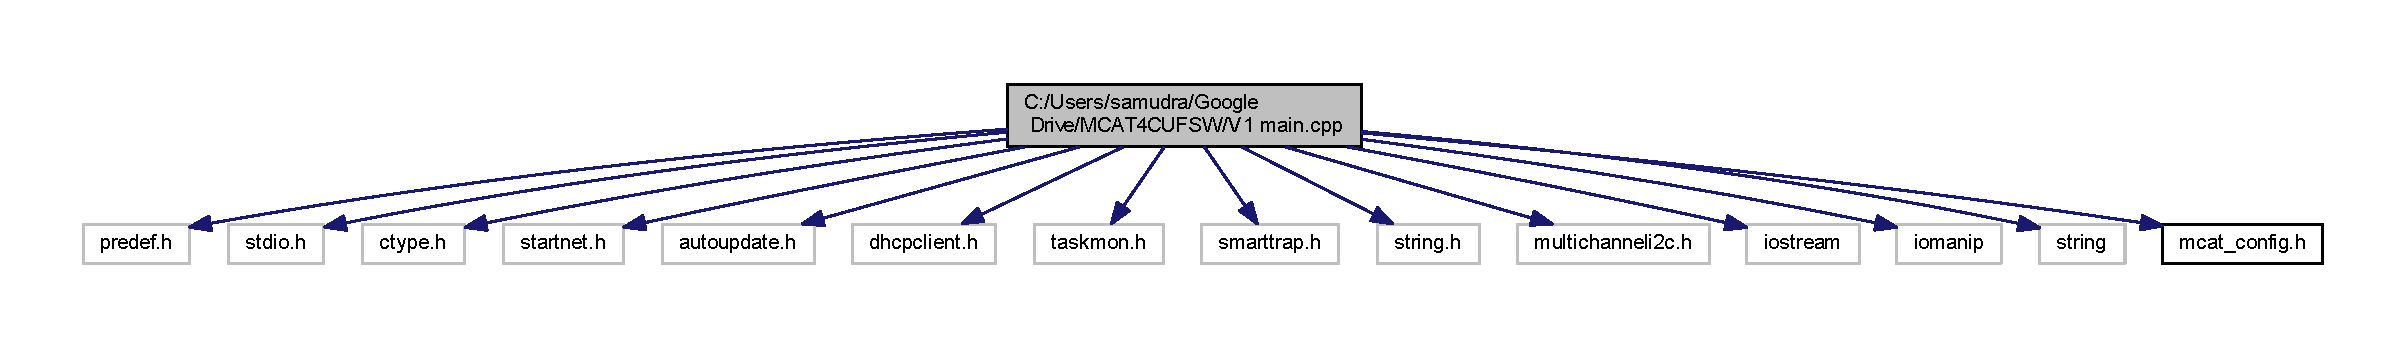
\includegraphics[width=350pt]{_v1_01main_8cpp__incl}
\end{center}
\end{figure}
\subsection*{Functions}
\begin{DoxyCompactItemize}
\item 
void \hyperlink{_v1_01main_8cpp_af3350bd69feae78ebcd4f766916eeb67}{parse\+C\+M\+D\+Packet} (char C\+M\+D\+Packet\mbox{[}I2\+C\+\_\+\+M\+A\+X\+\_\+\+B\+U\+F\+\_\+\+S\+I\+Z\+E\mbox{]})
\item 
void \hyperlink{_v1_01main_8cpp_aa3032893ba2f121a12d4cecf88277580}{parse\+Block\+G} (string Block\+G)
\item 
void \hyperlink{_v1_01main_8cpp_ab8ff54f4b027d2dfb6d3b63194fc15a4}{parse\+Block\+C\+U} (string Block\+C\+U)
\item 
void \hyperlink{_v1_01main_8cpp_a72e39dd7a2538b8b278f927ffd051bde}{parse\+Block\+I\+P\+D} (string Block\+I\+P\+D)
\item 
void \hyperlink{_v1_01main_8cpp_a8109658a433363943c469e7743c238ab}{parse\+Block\+P\+P\+U} (string Block\+P\+P\+U)
\item 
B\+Y\+T\+E \hyperlink{_v1_01main_8cpp_a22bb15ed96d4891d904b55838e451124}{Ascii2\+Byte} (char $\ast$buf)
\item 
void \hyperlink{_v1_01main_8cpp_ad16e5e62f3579a7048e6b981b172885e}{menu} (void)
\item 
void \hyperlink{_v1_01main_8cpp_ace7b2f4c33cbf41f3a43c7be01ff7aec}{User\+Main} (void $\ast$pd)
\end{DoxyCompactItemize}
\subsection*{Variables}
\begin{DoxyCompactItemize}
\item 
string \hyperlink{_v1_01main_8cpp_a405cdd34a0ec61abf8c5205c7a8c3182}{cmd\+Version} =\char`\"{}\char`\"{}
\item 
string \hyperlink{_v1_01main_8cpp_a8a9767341d04352fccd7068bc1d7c370}{cmd\+Mode} =\char`\"{}\char`\"{}
\item 
string \hyperlink{_v1_01main_8cpp_a56a16ee6139d263a1945acac7412db03}{s\+\_\+cmd\+T\+P1} =\char`\"{}\char`\"{}
\item 
string \hyperlink{_v1_01main_8cpp_ac2f7f3d71312267f0daf019326ab81ab}{s\+\_\+cmd\+T\+P2} =\char`\"{}\char`\"{}
\item 
string \hyperlink{_v1_01main_8cpp_a684796ab1de60babd3eba75aa8489e68}{s\+\_\+cmd\+T\+P3} =\char`\"{}\char`\"{}
\item 
string \hyperlink{_v1_01main_8cpp_a42269eac5fc051ca6c78aae8b6349920}{s\+\_\+cmd\+T\+P4} =\char`\"{}\char`\"{}
\item 
string \hyperlink{_v1_01main_8cpp_aa8cec591ab6bc2c30368790b9c90e439}{s\+\_\+cmd\+P\+C\+H1} =\char`\"{}\char`\"{}
\item 
string \hyperlink{_v1_01main_8cpp_a0f0135bb7a354979b68358781b0b9a33}{s\+\_\+cmd\+P\+C\+H2} =\char`\"{}\char`\"{}
\item 
string \hyperlink{_v1_01main_8cpp_ad027927effdfbc03356897f6784a332f}{s\+\_\+cmd\+P\+C\+H3} =\char`\"{}\char`\"{}
\item 
string \hyperlink{_v1_01main_8cpp_a1ee9de883e3c6e7840f6bfd0fdff6976}{s\+\_\+cmd\+P\+C\+H4} =\char`\"{}\char`\"{}
\item 
long \hyperlink{_v1_01main_8cpp_ac244c5de67ae1cf2ad9042dd3dd42f5c}{cmd\+T\+P1}
\item 
long \hyperlink{_v1_01main_8cpp_a6b5cb6b3c68ceba258ad6741ccf2c2c2}{cmd\+T\+P2}
\item 
long \hyperlink{_v1_01main_8cpp_a22ed1f6fb6c9e5132174497269472950}{cmd\+T\+P3}
\item 
long \hyperlink{_v1_01main_8cpp_ac556ac861b98bb773707ad78139dd4a7}{cmd\+T\+P4}
\item 
long \hyperlink{_v1_01main_8cpp_a6aa9310d261695da6caf50707b289e99}{cmd\+P\+C\+H1}
\item 
long \hyperlink{_v1_01main_8cpp_a2ede701ffcc3766012be6e4080433432}{cmd\+P\+C\+H2}
\item 
long \hyperlink{_v1_01main_8cpp_a5128aa37f4fea97bace715bd297c7cb4}{cmd\+P\+C\+H3}
\item 
long \hyperlink{_v1_01main_8cpp_acda88eaa3c77c003b3a5642a3e28bb48}{cmd\+P\+C\+H4}
\item 
string \hyperlink{_v1_01main_8cpp_a37ec136ae86c4b7dc81f393bb1a01af7}{s\+\_\+cmd\+P18\+H1} =\char`\"{}\char`\"{}
\item 
string \hyperlink{_v1_01main_8cpp_a46ce373f60085f5900464cd0731fa20e}{s\+\_\+cmd\+P18\+H2} =\char`\"{}\char`\"{}
\item 
string \hyperlink{_v1_01main_8cpp_a909acdc96889fb5885793e8bc70b083e}{s\+\_\+cmd\+P18\+H3} =\char`\"{}\char`\"{}
\item 
string \hyperlink{_v1_01main_8cpp_a607e82175ad61b864bfa84e686437947}{s\+\_\+cmd\+P18\+H4} =\char`\"{}\char`\"{}
\item 
bool \hyperlink{_v1_01main_8cpp_a1a10d6a42e7c3ba1ad7f396b687a7eb7}{cmd\+P18\+H1}
\item 
bool \hyperlink{_v1_01main_8cpp_a03df8cc8ee6b4d7ba8a3d2ad50914508}{cmd\+P18\+H2}
\item 
bool \hyperlink{_v1_01main_8cpp_aba803fecbea259c5af71f0b9f2e9fa5a}{cmd\+P18\+H3}
\item 
bool \hyperlink{_v1_01main_8cpp_a74d16dd0ede9be1a1645027bd2e6fb21}{cmd\+P18\+H4}
\item 
B\+Y\+T\+E \hyperlink{_v1_01main_8cpp_a750abfb0120c1735c922980bd47640a5}{buffer} \mbox{[}I2\+C\+\_\+\+M\+A\+X\+\_\+\+B\+U\+F\+\_\+\+S\+I\+Z\+E\mbox{]}
\item 
char \hyperlink{_v1_01main_8cpp_af54d77a991da4ba360d594c2589140df}{I2\+C\+Input\+Buffer} \mbox{[}I2\+C\+\_\+\+M\+A\+X\+\_\+\+B\+U\+F\+\_\+\+S\+I\+Z\+E\mbox{]}
\item 
char $\ast$ \hyperlink{_v1_01main_8cpp_abed0c40696905e144ed4118061acf700}{inbuf} = \hyperlink{_v2_01main_8cpp_af54d77a991da4ba360d594c2589140df}{I2\+C\+Input\+Buffer}
\item 
B\+Y\+T\+E \hyperlink{_v1_01main_8cpp_a92fb5ea5b6a7d108dea33dd07809152d}{address} = \hyperlink{mcatsubsystemconfig_8h_a8fe248bd745b90e2bfe94d8c5fce0a53}{C\+U\+\_\+\+I2\+C\+\_\+\+S\+L\+A\+V\+E\+\_\+\+A\+D\+D\+R}
\item 
B\+Y\+T\+E \hyperlink{_v1_01main_8cpp_a6c3dedd37414833dd07e72ee4a642d13}{I2\+C\+Stat}
\end{DoxyCompactItemize}


\subsection{Function Documentation}
\hypertarget{_v1_01main_8cpp_a22bb15ed96d4891d904b55838e451124}{}\index{V1 main.\+cpp@{V1 main.\+cpp}!Ascii2\+Byte@{Ascii2\+Byte}}
\index{Ascii2\+Byte@{Ascii2\+Byte}!V1 main.\+cpp@{V1 main.\+cpp}}
\subsubsection[{Ascii2\+Byte}]{\setlength{\rightskip}{0pt plus 5cm}B\+Y\+T\+E Ascii2\+Byte (
\begin{DoxyParamCaption}
\item[{char $\ast$}]{buf}
\end{DoxyParamCaption}
)}\label{_v1_01main_8cpp_a22bb15ed96d4891d904b55838e451124}


Definition at line 470 of file V1 main.\+cpp.

\hypertarget{_v1_01main_8cpp_ad16e5e62f3579a7048e6b981b172885e}{}\index{V1 main.\+cpp@{V1 main.\+cpp}!menu@{menu}}
\index{menu@{menu}!V1 main.\+cpp@{V1 main.\+cpp}}
\subsubsection[{menu}]{\setlength{\rightskip}{0pt plus 5cm}void menu (
\begin{DoxyParamCaption}
\item[{void}]{}
\end{DoxyParamCaption}
)}\label{_v1_01main_8cpp_ad16e5e62f3579a7048e6b981b172885e}


Definition at line 488 of file V1 main.\+cpp.

\hypertarget{_v1_01main_8cpp_ab8ff54f4b027d2dfb6d3b63194fc15a4}{}\index{V1 main.\+cpp@{V1 main.\+cpp}!parse\+Block\+C\+U@{parse\+Block\+C\+U}}
\index{parse\+Block\+C\+U@{parse\+Block\+C\+U}!V1 main.\+cpp@{V1 main.\+cpp}}
\subsubsection[{parse\+Block\+C\+U}]{\setlength{\rightskip}{0pt plus 5cm}void parse\+Block\+C\+U (
\begin{DoxyParamCaption}
\item[{string}]{Block\+C\+U}
\end{DoxyParamCaption}
)}\label{_v1_01main_8cpp_ab8ff54f4b027d2dfb6d3b63194fc15a4}


Definition at line 348 of file V1 main.\+cpp.

\hypertarget{_v1_01main_8cpp_aa3032893ba2f121a12d4cecf88277580}{}\index{V1 main.\+cpp@{V1 main.\+cpp}!parse\+Block\+G@{parse\+Block\+G}}
\index{parse\+Block\+G@{parse\+Block\+G}!V1 main.\+cpp@{V1 main.\+cpp}}
\subsubsection[{parse\+Block\+G}]{\setlength{\rightskip}{0pt plus 5cm}void parse\+Block\+G (
\begin{DoxyParamCaption}
\item[{string}]{Block\+G}
\end{DoxyParamCaption}
)}\label{_v1_01main_8cpp_aa3032893ba2f121a12d4cecf88277580}


Definition at line 338 of file V1 main.\+cpp.

\hypertarget{_v1_01main_8cpp_a72e39dd7a2538b8b278f927ffd051bde}{}\index{V1 main.\+cpp@{V1 main.\+cpp}!parse\+Block\+I\+P\+D@{parse\+Block\+I\+P\+D}}
\index{parse\+Block\+I\+P\+D@{parse\+Block\+I\+P\+D}!V1 main.\+cpp@{V1 main.\+cpp}}
\subsubsection[{parse\+Block\+I\+P\+D}]{\setlength{\rightskip}{0pt plus 5cm}void parse\+Block\+I\+P\+D (
\begin{DoxyParamCaption}
\item[{string}]{Block\+I\+P\+D}
\end{DoxyParamCaption}
)}\label{_v1_01main_8cpp_a72e39dd7a2538b8b278f927ffd051bde}


Definition at line 358 of file V1 main.\+cpp.

\hypertarget{_v1_01main_8cpp_a8109658a433363943c469e7743c238ab}{}\index{V1 main.\+cpp@{V1 main.\+cpp}!parse\+Block\+P\+P\+U@{parse\+Block\+P\+P\+U}}
\index{parse\+Block\+P\+P\+U@{parse\+Block\+P\+P\+U}!V1 main.\+cpp@{V1 main.\+cpp}}
\subsubsection[{parse\+Block\+P\+P\+U}]{\setlength{\rightskip}{0pt plus 5cm}void parse\+Block\+P\+P\+U (
\begin{DoxyParamCaption}
\item[{string}]{Block\+P\+P\+U}
\end{DoxyParamCaption}
)}\label{_v1_01main_8cpp_a8109658a433363943c469e7743c238ab}


Definition at line 413 of file V1 main.\+cpp.

\hypertarget{_v1_01main_8cpp_af3350bd69feae78ebcd4f766916eeb67}{}\index{V1 main.\+cpp@{V1 main.\+cpp}!parse\+C\+M\+D\+Packet@{parse\+C\+M\+D\+Packet}}
\index{parse\+C\+M\+D\+Packet@{parse\+C\+M\+D\+Packet}!V1 main.\+cpp@{V1 main.\+cpp}}
\subsubsection[{parse\+C\+M\+D\+Packet}]{\setlength{\rightskip}{0pt plus 5cm}void parse\+C\+M\+D\+Packet (
\begin{DoxyParamCaption}
\item[{char}]{C\+M\+D\+Packet\mbox{[}\+I2\+C\+\_\+\+M\+A\+X\+\_\+\+B\+U\+F\+\_\+\+S\+I\+Z\+E\mbox{]}}
\end{DoxyParamCaption}
)}\label{_v1_01main_8cpp_af3350bd69feae78ebcd4f766916eeb67}


Definition at line 284 of file V1 main.\+cpp.

\hypertarget{_v1_01main_8cpp_ace7b2f4c33cbf41f3a43c7be01ff7aec}{}\index{V1 main.\+cpp@{V1 main.\+cpp}!User\+Main@{User\+Main}}
\index{User\+Main@{User\+Main}!V1 main.\+cpp@{V1 main.\+cpp}}
\subsubsection[{User\+Main}]{\setlength{\rightskip}{0pt plus 5cm}void User\+Main (
\begin{DoxyParamCaption}
\item[{void $\ast$}]{pd}
\end{DoxyParamCaption}
)}\label{_v1_01main_8cpp_ace7b2f4c33cbf41f3a43c7be01ff7aec}


Definition at line 147 of file V1 main.\+cpp.



\subsection{Variable Documentation}
\hypertarget{_v1_01main_8cpp_a92fb5ea5b6a7d108dea33dd07809152d}{}\index{V1 main.\+cpp@{V1 main.\+cpp}!address@{address}}
\index{address@{address}!V1 main.\+cpp@{V1 main.\+cpp}}
\subsubsection[{address}]{\setlength{\rightskip}{0pt plus 5cm}B\+Y\+T\+E address = {\bf C\+U\+\_\+\+I2\+C\+\_\+\+S\+L\+A\+V\+E\+\_\+\+A\+D\+D\+R}}\label{_v1_01main_8cpp_a92fb5ea5b6a7d108dea33dd07809152d}


Definition at line 141 of file V1 main.\+cpp.

\hypertarget{_v1_01main_8cpp_a750abfb0120c1735c922980bd47640a5}{}\index{V1 main.\+cpp@{V1 main.\+cpp}!buffer@{buffer}}
\index{buffer@{buffer}!V1 main.\+cpp@{V1 main.\+cpp}}
\subsubsection[{buffer}]{\setlength{\rightskip}{0pt plus 5cm}B\+Y\+T\+E buffer\mbox{[}I2\+C\+\_\+\+M\+A\+X\+\_\+\+B\+U\+F\+\_\+\+S\+I\+Z\+E\mbox{]}}\label{_v1_01main_8cpp_a750abfb0120c1735c922980bd47640a5}


Definition at line 138 of file V1 main.\+cpp.

\hypertarget{_v1_01main_8cpp_a8a9767341d04352fccd7068bc1d7c370}{}\index{V1 main.\+cpp@{V1 main.\+cpp}!cmd\+Mode@{cmd\+Mode}}
\index{cmd\+Mode@{cmd\+Mode}!V1 main.\+cpp@{V1 main.\+cpp}}
\subsubsection[{cmd\+Mode}]{\setlength{\rightskip}{0pt plus 5cm}string cmd\+Mode =\char`\"{}\char`\"{}}\label{_v1_01main_8cpp_a8a9767341d04352fccd7068bc1d7c370}


Definition at line 92 of file V1 main.\+cpp.

\hypertarget{_v1_01main_8cpp_a1a10d6a42e7c3ba1ad7f396b687a7eb7}{}\index{V1 main.\+cpp@{V1 main.\+cpp}!cmd\+P18\+H1@{cmd\+P18\+H1}}
\index{cmd\+P18\+H1@{cmd\+P18\+H1}!V1 main.\+cpp@{V1 main.\+cpp}}
\subsubsection[{cmd\+P18\+H1}]{\setlength{\rightskip}{0pt plus 5cm}bool cmd\+P18\+H1}\label{_v1_01main_8cpp_a1a10d6a42e7c3ba1ad7f396b687a7eb7}


Definition at line 106 of file V1 main.\+cpp.

\hypertarget{_v1_01main_8cpp_a03df8cc8ee6b4d7ba8a3d2ad50914508}{}\index{V1 main.\+cpp@{V1 main.\+cpp}!cmd\+P18\+H2@{cmd\+P18\+H2}}
\index{cmd\+P18\+H2@{cmd\+P18\+H2}!V1 main.\+cpp@{V1 main.\+cpp}}
\subsubsection[{cmd\+P18\+H2}]{\setlength{\rightskip}{0pt plus 5cm}bool cmd\+P18\+H2}\label{_v1_01main_8cpp_a03df8cc8ee6b4d7ba8a3d2ad50914508}


Definition at line 106 of file V1 main.\+cpp.

\hypertarget{_v1_01main_8cpp_aba803fecbea259c5af71f0b9f2e9fa5a}{}\index{V1 main.\+cpp@{V1 main.\+cpp}!cmd\+P18\+H3@{cmd\+P18\+H3}}
\index{cmd\+P18\+H3@{cmd\+P18\+H3}!V1 main.\+cpp@{V1 main.\+cpp}}
\subsubsection[{cmd\+P18\+H3}]{\setlength{\rightskip}{0pt plus 5cm}bool cmd\+P18\+H3}\label{_v1_01main_8cpp_aba803fecbea259c5af71f0b9f2e9fa5a}


Definition at line 106 of file V1 main.\+cpp.

\hypertarget{_v1_01main_8cpp_a74d16dd0ede9be1a1645027bd2e6fb21}{}\index{V1 main.\+cpp@{V1 main.\+cpp}!cmd\+P18\+H4@{cmd\+P18\+H4}}
\index{cmd\+P18\+H4@{cmd\+P18\+H4}!V1 main.\+cpp@{V1 main.\+cpp}}
\subsubsection[{cmd\+P18\+H4}]{\setlength{\rightskip}{0pt plus 5cm}bool cmd\+P18\+H4}\label{_v1_01main_8cpp_a74d16dd0ede9be1a1645027bd2e6fb21}


Definition at line 106 of file V1 main.\+cpp.

\hypertarget{_v1_01main_8cpp_a6aa9310d261695da6caf50707b289e99}{}\index{V1 main.\+cpp@{V1 main.\+cpp}!cmd\+P\+C\+H1@{cmd\+P\+C\+H1}}
\index{cmd\+P\+C\+H1@{cmd\+P\+C\+H1}!V1 main.\+cpp@{V1 main.\+cpp}}
\subsubsection[{cmd\+P\+C\+H1}]{\setlength{\rightskip}{0pt plus 5cm}long cmd\+P\+C\+H1}\label{_v1_01main_8cpp_a6aa9310d261695da6caf50707b289e99}


Definition at line 101 of file V1 main.\+cpp.

\hypertarget{_v1_01main_8cpp_a2ede701ffcc3766012be6e4080433432}{}\index{V1 main.\+cpp@{V1 main.\+cpp}!cmd\+P\+C\+H2@{cmd\+P\+C\+H2}}
\index{cmd\+P\+C\+H2@{cmd\+P\+C\+H2}!V1 main.\+cpp@{V1 main.\+cpp}}
\subsubsection[{cmd\+P\+C\+H2}]{\setlength{\rightskip}{0pt plus 5cm}long cmd\+P\+C\+H2}\label{_v1_01main_8cpp_a2ede701ffcc3766012be6e4080433432}


Definition at line 101 of file V1 main.\+cpp.

\hypertarget{_v1_01main_8cpp_a5128aa37f4fea97bace715bd297c7cb4}{}\index{V1 main.\+cpp@{V1 main.\+cpp}!cmd\+P\+C\+H3@{cmd\+P\+C\+H3}}
\index{cmd\+P\+C\+H3@{cmd\+P\+C\+H3}!V1 main.\+cpp@{V1 main.\+cpp}}
\subsubsection[{cmd\+P\+C\+H3}]{\setlength{\rightskip}{0pt plus 5cm}long cmd\+P\+C\+H3}\label{_v1_01main_8cpp_a5128aa37f4fea97bace715bd297c7cb4}


Definition at line 101 of file V1 main.\+cpp.

\hypertarget{_v1_01main_8cpp_acda88eaa3c77c003b3a5642a3e28bb48}{}\index{V1 main.\+cpp@{V1 main.\+cpp}!cmd\+P\+C\+H4@{cmd\+P\+C\+H4}}
\index{cmd\+P\+C\+H4@{cmd\+P\+C\+H4}!V1 main.\+cpp@{V1 main.\+cpp}}
\subsubsection[{cmd\+P\+C\+H4}]{\setlength{\rightskip}{0pt plus 5cm}long cmd\+P\+C\+H4}\label{_v1_01main_8cpp_acda88eaa3c77c003b3a5642a3e28bb48}


Definition at line 101 of file V1 main.\+cpp.

\hypertarget{_v1_01main_8cpp_ac244c5de67ae1cf2ad9042dd3dd42f5c}{}\index{V1 main.\+cpp@{V1 main.\+cpp}!cmd\+T\+P1@{cmd\+T\+P1}}
\index{cmd\+T\+P1@{cmd\+T\+P1}!V1 main.\+cpp@{V1 main.\+cpp}}
\subsubsection[{cmd\+T\+P1}]{\setlength{\rightskip}{0pt plus 5cm}long cmd\+T\+P1}\label{_v1_01main_8cpp_ac244c5de67ae1cf2ad9042dd3dd42f5c}


Definition at line 101 of file V1 main.\+cpp.

\hypertarget{_v1_01main_8cpp_a6b5cb6b3c68ceba258ad6741ccf2c2c2}{}\index{V1 main.\+cpp@{V1 main.\+cpp}!cmd\+T\+P2@{cmd\+T\+P2}}
\index{cmd\+T\+P2@{cmd\+T\+P2}!V1 main.\+cpp@{V1 main.\+cpp}}
\subsubsection[{cmd\+T\+P2}]{\setlength{\rightskip}{0pt plus 5cm}long cmd\+T\+P2}\label{_v1_01main_8cpp_a6b5cb6b3c68ceba258ad6741ccf2c2c2}


Definition at line 101 of file V1 main.\+cpp.

\hypertarget{_v1_01main_8cpp_a22ed1f6fb6c9e5132174497269472950}{}\index{V1 main.\+cpp@{V1 main.\+cpp}!cmd\+T\+P3@{cmd\+T\+P3}}
\index{cmd\+T\+P3@{cmd\+T\+P3}!V1 main.\+cpp@{V1 main.\+cpp}}
\subsubsection[{cmd\+T\+P3}]{\setlength{\rightskip}{0pt plus 5cm}long cmd\+T\+P3}\label{_v1_01main_8cpp_a22ed1f6fb6c9e5132174497269472950}


Definition at line 101 of file V1 main.\+cpp.

\hypertarget{_v1_01main_8cpp_ac556ac861b98bb773707ad78139dd4a7}{}\index{V1 main.\+cpp@{V1 main.\+cpp}!cmd\+T\+P4@{cmd\+T\+P4}}
\index{cmd\+T\+P4@{cmd\+T\+P4}!V1 main.\+cpp@{V1 main.\+cpp}}
\subsubsection[{cmd\+T\+P4}]{\setlength{\rightskip}{0pt plus 5cm}long cmd\+T\+P4}\label{_v1_01main_8cpp_ac556ac861b98bb773707ad78139dd4a7}


Definition at line 101 of file V1 main.\+cpp.

\hypertarget{_v1_01main_8cpp_a405cdd34a0ec61abf8c5205c7a8c3182}{}\index{V1 main.\+cpp@{V1 main.\+cpp}!cmd\+Version@{cmd\+Version}}
\index{cmd\+Version@{cmd\+Version}!V1 main.\+cpp@{V1 main.\+cpp}}
\subsubsection[{cmd\+Version}]{\setlength{\rightskip}{0pt plus 5cm}string cmd\+Version =\char`\"{}\char`\"{}}\label{_v1_01main_8cpp_a405cdd34a0ec61abf8c5205c7a8c3182}


Definition at line 91 of file V1 main.\+cpp.

\hypertarget{_v1_01main_8cpp_af54d77a991da4ba360d594c2589140df}{}\index{V1 main.\+cpp@{V1 main.\+cpp}!I2\+C\+Input\+Buffer@{I2\+C\+Input\+Buffer}}
\index{I2\+C\+Input\+Buffer@{I2\+C\+Input\+Buffer}!V1 main.\+cpp@{V1 main.\+cpp}}
\subsubsection[{I2\+C\+Input\+Buffer}]{\setlength{\rightskip}{0pt plus 5cm}char I2\+C\+Input\+Buffer\mbox{[}I2\+C\+\_\+\+M\+A\+X\+\_\+\+B\+U\+F\+\_\+\+S\+I\+Z\+E\mbox{]}}\label{_v1_01main_8cpp_af54d77a991da4ba360d594c2589140df}


Definition at line 139 of file V1 main.\+cpp.

\hypertarget{_v1_01main_8cpp_a6c3dedd37414833dd07e72ee4a642d13}{}\index{V1 main.\+cpp@{V1 main.\+cpp}!I2\+C\+Stat@{I2\+C\+Stat}}
\index{I2\+C\+Stat@{I2\+C\+Stat}!V1 main.\+cpp@{V1 main.\+cpp}}
\subsubsection[{I2\+C\+Stat}]{\setlength{\rightskip}{0pt plus 5cm}B\+Y\+T\+E I2\+C\+Stat}\label{_v1_01main_8cpp_a6c3dedd37414833dd07e72ee4a642d13}


Definition at line 142 of file V1 main.\+cpp.

\hypertarget{_v1_01main_8cpp_abed0c40696905e144ed4118061acf700}{}\index{V1 main.\+cpp@{V1 main.\+cpp}!inbuf@{inbuf}}
\index{inbuf@{inbuf}!V1 main.\+cpp@{V1 main.\+cpp}}
\subsubsection[{inbuf}]{\setlength{\rightskip}{0pt plus 5cm}char$\ast$ inbuf = {\bf I2\+C\+Input\+Buffer}}\label{_v1_01main_8cpp_abed0c40696905e144ed4118061acf700}


Definition at line 140 of file V1 main.\+cpp.

\hypertarget{_v1_01main_8cpp_a37ec136ae86c4b7dc81f393bb1a01af7}{}\index{V1 main.\+cpp@{V1 main.\+cpp}!s\+\_\+cmd\+P18\+H1@{s\+\_\+cmd\+P18\+H1}}
\index{s\+\_\+cmd\+P18\+H1@{s\+\_\+cmd\+P18\+H1}!V1 main.\+cpp@{V1 main.\+cpp}}
\subsubsection[{s\+\_\+cmd\+P18\+H1}]{\setlength{\rightskip}{0pt plus 5cm}string s\+\_\+cmd\+P18\+H1 =\char`\"{}\char`\"{}}\label{_v1_01main_8cpp_a37ec136ae86c4b7dc81f393bb1a01af7}


Definition at line 102 of file V1 main.\+cpp.

\hypertarget{_v1_01main_8cpp_a46ce373f60085f5900464cd0731fa20e}{}\index{V1 main.\+cpp@{V1 main.\+cpp}!s\+\_\+cmd\+P18\+H2@{s\+\_\+cmd\+P18\+H2}}
\index{s\+\_\+cmd\+P18\+H2@{s\+\_\+cmd\+P18\+H2}!V1 main.\+cpp@{V1 main.\+cpp}}
\subsubsection[{s\+\_\+cmd\+P18\+H2}]{\setlength{\rightskip}{0pt plus 5cm}string s\+\_\+cmd\+P18\+H2 =\char`\"{}\char`\"{}}\label{_v1_01main_8cpp_a46ce373f60085f5900464cd0731fa20e}


Definition at line 103 of file V1 main.\+cpp.

\hypertarget{_v1_01main_8cpp_a909acdc96889fb5885793e8bc70b083e}{}\index{V1 main.\+cpp@{V1 main.\+cpp}!s\+\_\+cmd\+P18\+H3@{s\+\_\+cmd\+P18\+H3}}
\index{s\+\_\+cmd\+P18\+H3@{s\+\_\+cmd\+P18\+H3}!V1 main.\+cpp@{V1 main.\+cpp}}
\subsubsection[{s\+\_\+cmd\+P18\+H3}]{\setlength{\rightskip}{0pt plus 5cm}string s\+\_\+cmd\+P18\+H3 =\char`\"{}\char`\"{}}\label{_v1_01main_8cpp_a909acdc96889fb5885793e8bc70b083e}


Definition at line 104 of file V1 main.\+cpp.

\hypertarget{_v1_01main_8cpp_a607e82175ad61b864bfa84e686437947}{}\index{V1 main.\+cpp@{V1 main.\+cpp}!s\+\_\+cmd\+P18\+H4@{s\+\_\+cmd\+P18\+H4}}
\index{s\+\_\+cmd\+P18\+H4@{s\+\_\+cmd\+P18\+H4}!V1 main.\+cpp@{V1 main.\+cpp}}
\subsubsection[{s\+\_\+cmd\+P18\+H4}]{\setlength{\rightskip}{0pt plus 5cm}string s\+\_\+cmd\+P18\+H4 =\char`\"{}\char`\"{}}\label{_v1_01main_8cpp_a607e82175ad61b864bfa84e686437947}


Definition at line 105 of file V1 main.\+cpp.

\hypertarget{_v1_01main_8cpp_aa8cec591ab6bc2c30368790b9c90e439}{}\index{V1 main.\+cpp@{V1 main.\+cpp}!s\+\_\+cmd\+P\+C\+H1@{s\+\_\+cmd\+P\+C\+H1}}
\index{s\+\_\+cmd\+P\+C\+H1@{s\+\_\+cmd\+P\+C\+H1}!V1 main.\+cpp@{V1 main.\+cpp}}
\subsubsection[{s\+\_\+cmd\+P\+C\+H1}]{\setlength{\rightskip}{0pt plus 5cm}string s\+\_\+cmd\+P\+C\+H1 =\char`\"{}\char`\"{}}\label{_v1_01main_8cpp_aa8cec591ab6bc2c30368790b9c90e439}


Definition at line 97 of file V1 main.\+cpp.

\hypertarget{_v1_01main_8cpp_a0f0135bb7a354979b68358781b0b9a33}{}\index{V1 main.\+cpp@{V1 main.\+cpp}!s\+\_\+cmd\+P\+C\+H2@{s\+\_\+cmd\+P\+C\+H2}}
\index{s\+\_\+cmd\+P\+C\+H2@{s\+\_\+cmd\+P\+C\+H2}!V1 main.\+cpp@{V1 main.\+cpp}}
\subsubsection[{s\+\_\+cmd\+P\+C\+H2}]{\setlength{\rightskip}{0pt plus 5cm}string s\+\_\+cmd\+P\+C\+H2 =\char`\"{}\char`\"{}}\label{_v1_01main_8cpp_a0f0135bb7a354979b68358781b0b9a33}


Definition at line 98 of file V1 main.\+cpp.

\hypertarget{_v1_01main_8cpp_ad027927effdfbc03356897f6784a332f}{}\index{V1 main.\+cpp@{V1 main.\+cpp}!s\+\_\+cmd\+P\+C\+H3@{s\+\_\+cmd\+P\+C\+H3}}
\index{s\+\_\+cmd\+P\+C\+H3@{s\+\_\+cmd\+P\+C\+H3}!V1 main.\+cpp@{V1 main.\+cpp}}
\subsubsection[{s\+\_\+cmd\+P\+C\+H3}]{\setlength{\rightskip}{0pt plus 5cm}string s\+\_\+cmd\+P\+C\+H3 =\char`\"{}\char`\"{}}\label{_v1_01main_8cpp_ad027927effdfbc03356897f6784a332f}


Definition at line 99 of file V1 main.\+cpp.

\hypertarget{_v1_01main_8cpp_a1ee9de883e3c6e7840f6bfd0fdff6976}{}\index{V1 main.\+cpp@{V1 main.\+cpp}!s\+\_\+cmd\+P\+C\+H4@{s\+\_\+cmd\+P\+C\+H4}}
\index{s\+\_\+cmd\+P\+C\+H4@{s\+\_\+cmd\+P\+C\+H4}!V1 main.\+cpp@{V1 main.\+cpp}}
\subsubsection[{s\+\_\+cmd\+P\+C\+H4}]{\setlength{\rightskip}{0pt plus 5cm}string s\+\_\+cmd\+P\+C\+H4 =\char`\"{}\char`\"{}}\label{_v1_01main_8cpp_a1ee9de883e3c6e7840f6bfd0fdff6976}


Definition at line 100 of file V1 main.\+cpp.

\hypertarget{_v1_01main_8cpp_a56a16ee6139d263a1945acac7412db03}{}\index{V1 main.\+cpp@{V1 main.\+cpp}!s\+\_\+cmd\+T\+P1@{s\+\_\+cmd\+T\+P1}}
\index{s\+\_\+cmd\+T\+P1@{s\+\_\+cmd\+T\+P1}!V1 main.\+cpp@{V1 main.\+cpp}}
\subsubsection[{s\+\_\+cmd\+T\+P1}]{\setlength{\rightskip}{0pt plus 5cm}string s\+\_\+cmd\+T\+P1 =\char`\"{}\char`\"{}}\label{_v1_01main_8cpp_a56a16ee6139d263a1945acac7412db03}


Definition at line 93 of file V1 main.\+cpp.

\hypertarget{_v1_01main_8cpp_ac2f7f3d71312267f0daf019326ab81ab}{}\index{V1 main.\+cpp@{V1 main.\+cpp}!s\+\_\+cmd\+T\+P2@{s\+\_\+cmd\+T\+P2}}
\index{s\+\_\+cmd\+T\+P2@{s\+\_\+cmd\+T\+P2}!V1 main.\+cpp@{V1 main.\+cpp}}
\subsubsection[{s\+\_\+cmd\+T\+P2}]{\setlength{\rightskip}{0pt plus 5cm}string s\+\_\+cmd\+T\+P2 =\char`\"{}\char`\"{}}\label{_v1_01main_8cpp_ac2f7f3d71312267f0daf019326ab81ab}


Definition at line 94 of file V1 main.\+cpp.

\hypertarget{_v1_01main_8cpp_a684796ab1de60babd3eba75aa8489e68}{}\index{V1 main.\+cpp@{V1 main.\+cpp}!s\+\_\+cmd\+T\+P3@{s\+\_\+cmd\+T\+P3}}
\index{s\+\_\+cmd\+T\+P3@{s\+\_\+cmd\+T\+P3}!V1 main.\+cpp@{V1 main.\+cpp}}
\subsubsection[{s\+\_\+cmd\+T\+P3}]{\setlength{\rightskip}{0pt plus 5cm}string s\+\_\+cmd\+T\+P3 =\char`\"{}\char`\"{}}\label{_v1_01main_8cpp_a684796ab1de60babd3eba75aa8489e68}


Definition at line 95 of file V1 main.\+cpp.

\hypertarget{_v1_01main_8cpp_a42269eac5fc051ca6c78aae8b6349920}{}\index{V1 main.\+cpp@{V1 main.\+cpp}!s\+\_\+cmd\+T\+P4@{s\+\_\+cmd\+T\+P4}}
\index{s\+\_\+cmd\+T\+P4@{s\+\_\+cmd\+T\+P4}!V1 main.\+cpp@{V1 main.\+cpp}}
\subsubsection[{s\+\_\+cmd\+T\+P4}]{\setlength{\rightskip}{0pt plus 5cm}string s\+\_\+cmd\+T\+P4 =\char`\"{}\char`\"{}}\label{_v1_01main_8cpp_a42269eac5fc051ca6c78aae8b6349920}


Definition at line 96 of file V1 main.\+cpp.


\hypertarget{_v2_01main_8cpp}{}\section{C\+:/\+Users/samudra/\+Google Drive/\+M\+C\+A\+T4\+C\+U\+F\+S\+W/\+V2 main.\+cpp File Reference}
\label{_v2_01main_8cpp}\index{C\+:/\+Users/samudra/\+Google Drive/\+M\+C\+A\+T4\+C\+U\+F\+S\+W/\+V2 main.\+cpp@{C\+:/\+Users/samudra/\+Google Drive/\+M\+C\+A\+T4\+C\+U\+F\+S\+W/\+V2 main.\+cpp}}
{\ttfamily \#include \char`\"{}predef.\+h\char`\"{}}\\*
{\ttfamily \#include $<$stdio.\+h$>$}\\*
{\ttfamily \#include $<$ctype.\+h$>$}\\*
{\ttfamily \#include $<$startnet.\+h$>$}\\*
{\ttfamily \#include $<$autoupdate.\+h$>$}\\*
{\ttfamily \#include $<$dhcpclient.\+h$>$}\\*
{\ttfamily \#include $<$taskmon.\+h$>$}\\*
{\ttfamily \#include $<$smarttrap.\+h$>$}\\*
{\ttfamily \#include $<$string.\+h$>$}\\*
{\ttfamily \#include $<$math.\+h$>$}\\*
{\ttfamily \#include $<$multichanneli2c.\+h$>$}\\*
{\ttfamily \#include $<$iostream$>$}\\*
{\ttfamily \#include $<$iomanip$>$}\\*
{\ttfamily \#include $<$string$>$}\\*
{\ttfamily \#include \char`\"{}mcat\+\_\+config.\+h\char`\"{}}\\*
Include dependency graph for V2 main.\+cpp\+:
\nopagebreak
\begin{figure}[H]
\begin{center}
\leavevmode
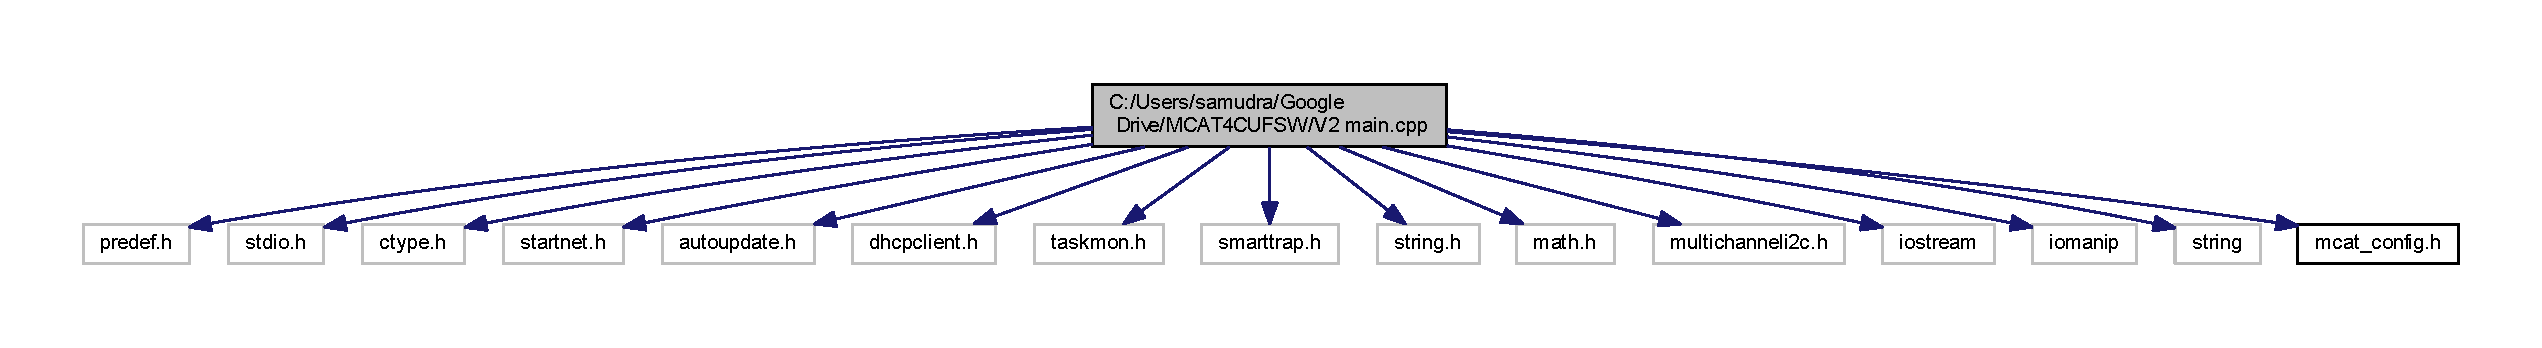
\includegraphics[width=350pt]{_v2_01main_8cpp__incl}
\end{center}
\end{figure}
\subsection*{Functions}
\begin{DoxyCompactItemize}
\item 
void \hyperlink{_v2_01main_8cpp_af3350bd69feae78ebcd4f766916eeb67}{parse\+C\+M\+D\+Packet} (char C\+M\+D\+Packet\mbox{[}I2\+C\+\_\+\+M\+A\+X\+\_\+\+B\+U\+F\+\_\+\+S\+I\+Z\+E\mbox{]})
\item 
void \hyperlink{_v2_01main_8cpp_aa3032893ba2f121a12d4cecf88277580}{parse\+Block\+G} (string Block\+G)
\item 
void \hyperlink{_v2_01main_8cpp_ab8ff54f4b027d2dfb6d3b63194fc15a4}{parse\+Block\+C\+U} (string Block\+C\+U)
\item 
void \hyperlink{_v2_01main_8cpp_a72e39dd7a2538b8b278f927ffd051bde}{parse\+Block\+I\+P\+D} (string Block\+I\+P\+D)
\item 
void \hyperlink{_v2_01main_8cpp_a8109658a433363943c469e7743c238ab}{parse\+Block\+P\+P\+U} (string Block\+P\+P\+U)
\item 
B\+Y\+T\+E \hyperlink{_v2_01main_8cpp_a22bb15ed96d4891d904b55838e451124}{Ascii2\+Byte} (char $\ast$buf)
\item 
void \hyperlink{_v2_01main_8cpp_ad16e5e62f3579a7048e6b981b172885e}{menu} (void)
\item 
void \hyperlink{_v2_01main_8cpp_ace7b2f4c33cbf41f3a43c7be01ff7aec}{User\+Main} (void $\ast$pd)
\item 
void \hyperlink{_v2_01main_8cpp_aecd22dba5b4407d85b05640e853fc6f6}{display\+C\+L\+I\+Menu} ()
\item 
void \hyperlink{_v2_01main_8cpp_a486c7b37eb37847afaeeb6c73de398b9}{display\+Config} ()
\item 
void \hyperlink{_v2_01main_8cpp_a855e0d71fbad695926236f90ac687f35}{do\+Pulses} (void $\ast$pdata)
\item 
void \hyperlink{_v2_01main_8cpp_a11ee600b69b27b0bb2d1b5b6e8ece140}{stop\+Pulses} (void $\ast$pdata)
\item 
void \hyperlink{_v2_01main_8cpp_a10570e6420ce0f0a076e1e9d3518d305}{init\+D\+M\+A\+T\+I\+M\+E\+R1} ()
\item 
void \hyperlink{_v2_01main_8cpp_a7c3f73193878c079945a21075f128059}{Set\+Intc} (long func, int vector, int level, int prio)
\item 
void \hyperlink{_v2_01main_8cpp_a8a64466bfb43094b3aec845670b959b4}{set\+Defaults} ()
\item 
void \hyperlink{_v2_01main_8cpp_a238885c747f586049b766fa4fcd5ec12}{disable\+All} ()
\item 
\hyperlink{_v2_01main_8cpp_a89200d64c07024287b4ef31901f44e15}{I\+N\+T\+E\+R\+R\+U\+P\+T} (func\+\_\+isr, 0x2600)
\end{DoxyCompactItemize}
\subsection*{Variables}
\begin{DoxyCompactItemize}
\item 
string \hyperlink{_v2_01main_8cpp_a405cdd34a0ec61abf8c5205c7a8c3182}{cmd\+Version} =\char`\"{}\char`\"{}
\item 
string \hyperlink{_v2_01main_8cpp_a8a9767341d04352fccd7068bc1d7c370}{cmd\+Mode} =\char`\"{}\char`\"{}
\item 
string \hyperlink{_v2_01main_8cpp_a56a16ee6139d263a1945acac7412db03}{s\+\_\+cmd\+T\+P1} =\char`\"{}\char`\"{}
\item 
string \hyperlink{_v2_01main_8cpp_ac2f7f3d71312267f0daf019326ab81ab}{s\+\_\+cmd\+T\+P2} =\char`\"{}\char`\"{}
\item 
string \hyperlink{_v2_01main_8cpp_a684796ab1de60babd3eba75aa8489e68}{s\+\_\+cmd\+T\+P3} =\char`\"{}\char`\"{}
\item 
string \hyperlink{_v2_01main_8cpp_a42269eac5fc051ca6c78aae8b6349920}{s\+\_\+cmd\+T\+P4} =\char`\"{}\char`\"{}
\item 
string \hyperlink{_v2_01main_8cpp_aa8cec591ab6bc2c30368790b9c90e439}{s\+\_\+cmd\+P\+C\+H1} =\char`\"{}\char`\"{}
\item 
string \hyperlink{_v2_01main_8cpp_a0f0135bb7a354979b68358781b0b9a33}{s\+\_\+cmd\+P\+C\+H2} =\char`\"{}\char`\"{}
\item 
string \hyperlink{_v2_01main_8cpp_ad027927effdfbc03356897f6784a332f}{s\+\_\+cmd\+P\+C\+H3} =\char`\"{}\char`\"{}
\item 
string \hyperlink{_v2_01main_8cpp_a1ee9de883e3c6e7840f6bfd0fdff6976}{s\+\_\+cmd\+P\+C\+H4} =\char`\"{}\char`\"{}
\item 
long \hyperlink{_v2_01main_8cpp_ac244c5de67ae1cf2ad9042dd3dd42f5c}{cmd\+T\+P1}
\item 
long \hyperlink{_v2_01main_8cpp_a6b5cb6b3c68ceba258ad6741ccf2c2c2}{cmd\+T\+P2}
\item 
long \hyperlink{_v2_01main_8cpp_a22ed1f6fb6c9e5132174497269472950}{cmd\+T\+P3}
\item 
long \hyperlink{_v2_01main_8cpp_ac556ac861b98bb773707ad78139dd4a7}{cmd\+T\+P4}
\item 
long \hyperlink{_v2_01main_8cpp_a6aa9310d261695da6caf50707b289e99}{cmd\+P\+C\+H1}
\item 
long \hyperlink{_v2_01main_8cpp_a2ede701ffcc3766012be6e4080433432}{cmd\+P\+C\+H2}
\item 
long \hyperlink{_v2_01main_8cpp_a5128aa37f4fea97bace715bd297c7cb4}{cmd\+P\+C\+H3}
\item 
long \hyperlink{_v2_01main_8cpp_acda88eaa3c77c003b3a5642a3e28bb48}{cmd\+P\+C\+H4}
\item 
string \hyperlink{_v2_01main_8cpp_a37ec136ae86c4b7dc81f393bb1a01af7}{s\+\_\+cmd\+P18\+H1} =\char`\"{}\char`\"{}
\item 
string \hyperlink{_v2_01main_8cpp_a46ce373f60085f5900464cd0731fa20e}{s\+\_\+cmd\+P18\+H2} =\char`\"{}\char`\"{}
\item 
string \hyperlink{_v2_01main_8cpp_a909acdc96889fb5885793e8bc70b083e}{s\+\_\+cmd\+P18\+H3} =\char`\"{}\char`\"{}
\item 
string \hyperlink{_v2_01main_8cpp_a607e82175ad61b864bfa84e686437947}{s\+\_\+cmd\+P18\+H4} =\char`\"{}\char`\"{}
\item 
bool \hyperlink{_v2_01main_8cpp_a1a10d6a42e7c3ba1ad7f396b687a7eb7}{cmd\+P18\+H1}
\item 
bool \hyperlink{_v2_01main_8cpp_a03df8cc8ee6b4d7ba8a3d2ad50914508}{cmd\+P18\+H2}
\item 
bool \hyperlink{_v2_01main_8cpp_aba803fecbea259c5af71f0b9f2e9fa5a}{cmd\+P18\+H3}
\item 
bool \hyperlink{_v2_01main_8cpp_a74d16dd0ede9be1a1645027bd2e6fb21}{cmd\+P18\+H4}
\item 
B\+Y\+T\+E \hyperlink{_v2_01main_8cpp_a750abfb0120c1735c922980bd47640a5}{buffer} \mbox{[}I2\+C\+\_\+\+M\+A\+X\+\_\+\+B\+U\+F\+\_\+\+S\+I\+Z\+E\mbox{]}
\item 
char \hyperlink{_v2_01main_8cpp_af54d77a991da4ba360d594c2589140df}{I2\+C\+Input\+Buffer} \mbox{[}I2\+C\+\_\+\+M\+A\+X\+\_\+\+B\+U\+F\+\_\+\+S\+I\+Z\+E\mbox{]}
\item 
char $\ast$ \hyperlink{_v2_01main_8cpp_abed0c40696905e144ed4118061acf700}{inbuf} = \hyperlink{_v2_01main_8cpp_af54d77a991da4ba360d594c2589140df}{I2\+C\+Input\+Buffer}
\item 
B\+Y\+T\+E \hyperlink{_v2_01main_8cpp_a92fb5ea5b6a7d108dea33dd07809152d}{address} = \hyperlink{mcatsubsystemconfig_8h_a8fe248bd745b90e2bfe94d8c5fce0a53}{C\+U\+\_\+\+I2\+C\+\_\+\+S\+L\+A\+V\+E\+\_\+\+A\+D\+D\+R}
\item 
B\+Y\+T\+E \hyperlink{_v2_01main_8cpp_a6c3dedd37414833dd07e72ee4a642d13}{I2\+C\+Stat}
\end{DoxyCompactItemize}


\subsection{Function Documentation}
\hypertarget{_v2_01main_8cpp_a22bb15ed96d4891d904b55838e451124}{}\index{V2 main.\+cpp@{V2 main.\+cpp}!Ascii2\+Byte@{Ascii2\+Byte}}
\index{Ascii2\+Byte@{Ascii2\+Byte}!V2 main.\+cpp@{V2 main.\+cpp}}
\subsubsection[{Ascii2\+Byte}]{\setlength{\rightskip}{0pt plus 5cm}B\+Y\+T\+E Ascii2\+Byte (
\begin{DoxyParamCaption}
\item[{char $\ast$}]{buf}
\end{DoxyParamCaption}
)}\label{_v2_01main_8cpp_a22bb15ed96d4891d904b55838e451124}


Definition at line 691 of file V2 main.\+cpp.

\hypertarget{_v2_01main_8cpp_a238885c747f586049b766fa4fcd5ec12}{}\index{V2 main.\+cpp@{V2 main.\+cpp}!disable\+All@{disable\+All}}
\index{disable\+All@{disable\+All}!V2 main.\+cpp@{V2 main.\+cpp}}
\subsubsection[{disable\+All}]{\setlength{\rightskip}{0pt plus 5cm}void disable\+All (
\begin{DoxyParamCaption}
{}
\end{DoxyParamCaption}
)}\label{_v2_01main_8cpp_a238885c747f586049b766fa4fcd5ec12}


Definition at line 214 of file V2 main.\+cpp.

\hypertarget{_v2_01main_8cpp_aecd22dba5b4407d85b05640e853fc6f6}{}\index{V2 main.\+cpp@{V2 main.\+cpp}!display\+C\+L\+I\+Menu@{display\+C\+L\+I\+Menu}}
\index{display\+C\+L\+I\+Menu@{display\+C\+L\+I\+Menu}!V2 main.\+cpp@{V2 main.\+cpp}}
\subsubsection[{display\+C\+L\+I\+Menu}]{\setlength{\rightskip}{0pt plus 5cm}void display\+C\+L\+I\+Menu (
\begin{DoxyParamCaption}
{}
\end{DoxyParamCaption}
)}\label{_v2_01main_8cpp_aecd22dba5b4407d85b05640e853fc6f6}


Definition at line 259 of file V2 main.\+cpp.

\hypertarget{_v2_01main_8cpp_a486c7b37eb37847afaeeb6c73de398b9}{}\index{V2 main.\+cpp@{V2 main.\+cpp}!display\+Config@{display\+Config}}
\index{display\+Config@{display\+Config}!V2 main.\+cpp@{V2 main.\+cpp}}
\subsubsection[{display\+Config}]{\setlength{\rightskip}{0pt plus 5cm}void display\+Config (
\begin{DoxyParamCaption}
{}
\end{DoxyParamCaption}
)}\label{_v2_01main_8cpp_a486c7b37eb37847afaeeb6c73de398b9}
\hypertarget{_v2_01main_8cpp_a855e0d71fbad695926236f90ac687f35}{}\index{V2 main.\+cpp@{V2 main.\+cpp}!do\+Pulses@{do\+Pulses}}
\index{do\+Pulses@{do\+Pulses}!V2 main.\+cpp@{V2 main.\+cpp}}
\subsubsection[{do\+Pulses}]{\setlength{\rightskip}{0pt plus 5cm}void do\+Pulses (
\begin{DoxyParamCaption}
\item[{void $\ast$}]{pdata}
\end{DoxyParamCaption}
)}\label{_v2_01main_8cpp_a855e0d71fbad695926236f90ac687f35}


Definition at line 232 of file V2 main.\+cpp.

\hypertarget{_v2_01main_8cpp_a10570e6420ce0f0a076e1e9d3518d305}{}\index{V2 main.\+cpp@{V2 main.\+cpp}!init\+D\+M\+A\+T\+I\+M\+E\+R1@{init\+D\+M\+A\+T\+I\+M\+E\+R1}}
\index{init\+D\+M\+A\+T\+I\+M\+E\+R1@{init\+D\+M\+A\+T\+I\+M\+E\+R1}!V2 main.\+cpp@{V2 main.\+cpp}}
\subsubsection[{init\+D\+M\+A\+T\+I\+M\+E\+R1}]{\setlength{\rightskip}{0pt plus 5cm}void init\+D\+M\+A\+T\+I\+M\+E\+R1 (
\begin{DoxyParamCaption}
{}
\end{DoxyParamCaption}
)}\label{_v2_01main_8cpp_a10570e6420ce0f0a076e1e9d3518d305}
from 5270 code set /// D\+O N\+O\+T U\+S\+E Set\+Intc((long) \&func\+\_\+isr, 19, 1, 1);

from 5270 code set /// D\+O N\+O\+T U\+S\+E Set\+Intc((long) \&func\+\_\+isr, 19, 1, 1);

from 5270 code set /// D\+O N\+O\+T U\+S\+E Set\+Intc((long) \&func\+\_\+isr, 19, 1, 1); 

Definition at line 655 of file main5.\+cpp.

\hypertarget{_v2_01main_8cpp_a89200d64c07024287b4ef31901f44e15}{}\index{V2 main.\+cpp@{V2 main.\+cpp}!I\+N\+T\+E\+R\+R\+U\+P\+T@{I\+N\+T\+E\+R\+R\+U\+P\+T}}
\index{I\+N\+T\+E\+R\+R\+U\+P\+T@{I\+N\+T\+E\+R\+R\+U\+P\+T}!V2 main.\+cpp@{V2 main.\+cpp}}
\subsubsection[{I\+N\+T\+E\+R\+R\+U\+P\+T}]{\setlength{\rightskip}{0pt plus 5cm}I\+N\+T\+E\+R\+R\+U\+P\+T (
\begin{DoxyParamCaption}
\item[{func\+\_\+isr}]{, }
\item[{0x2600}]{}
\end{DoxyParamCaption}
)}\label{_v2_01main_8cpp_a89200d64c07024287b4ef31901f44e15}


Definition at line 164 of file V2 main.\+cpp.

\hypertarget{_v2_01main_8cpp_ad16e5e62f3579a7048e6b981b172885e}{}\index{V2 main.\+cpp@{V2 main.\+cpp}!menu@{menu}}
\index{menu@{menu}!V2 main.\+cpp@{V2 main.\+cpp}}
\subsubsection[{menu}]{\setlength{\rightskip}{0pt plus 5cm}void menu (
\begin{DoxyParamCaption}
\item[{void}]{}
\end{DoxyParamCaption}
)}\label{_v2_01main_8cpp_ad16e5e62f3579a7048e6b981b172885e}


Definition at line 709 of file V2 main.\+cpp.

\hypertarget{_v2_01main_8cpp_ab8ff54f4b027d2dfb6d3b63194fc15a4}{}\index{V2 main.\+cpp@{V2 main.\+cpp}!parse\+Block\+C\+U@{parse\+Block\+C\+U}}
\index{parse\+Block\+C\+U@{parse\+Block\+C\+U}!V2 main.\+cpp@{V2 main.\+cpp}}
\subsubsection[{parse\+Block\+C\+U}]{\setlength{\rightskip}{0pt plus 5cm}void parse\+Block\+C\+U (
\begin{DoxyParamCaption}
\item[{string}]{Block\+C\+U}
\end{DoxyParamCaption}
)}\label{_v2_01main_8cpp_ab8ff54f4b027d2dfb6d3b63194fc15a4}


Definition at line 569 of file V2 main.\+cpp.

\hypertarget{_v2_01main_8cpp_aa3032893ba2f121a12d4cecf88277580}{}\index{V2 main.\+cpp@{V2 main.\+cpp}!parse\+Block\+G@{parse\+Block\+G}}
\index{parse\+Block\+G@{parse\+Block\+G}!V2 main.\+cpp@{V2 main.\+cpp}}
\subsubsection[{parse\+Block\+G}]{\setlength{\rightskip}{0pt plus 5cm}void parse\+Block\+G (
\begin{DoxyParamCaption}
\item[{string}]{Block\+G}
\end{DoxyParamCaption}
)}\label{_v2_01main_8cpp_aa3032893ba2f121a12d4cecf88277580}


Definition at line 559 of file V2 main.\+cpp.

\hypertarget{_v2_01main_8cpp_a72e39dd7a2538b8b278f927ffd051bde}{}\index{V2 main.\+cpp@{V2 main.\+cpp}!parse\+Block\+I\+P\+D@{parse\+Block\+I\+P\+D}}
\index{parse\+Block\+I\+P\+D@{parse\+Block\+I\+P\+D}!V2 main.\+cpp@{V2 main.\+cpp}}
\subsubsection[{parse\+Block\+I\+P\+D}]{\setlength{\rightskip}{0pt plus 5cm}void parse\+Block\+I\+P\+D (
\begin{DoxyParamCaption}
\item[{string}]{Block\+I\+P\+D}
\end{DoxyParamCaption}
)}\label{_v2_01main_8cpp_a72e39dd7a2538b8b278f927ffd051bde}


Definition at line 579 of file V2 main.\+cpp.

\hypertarget{_v2_01main_8cpp_a8109658a433363943c469e7743c238ab}{}\index{V2 main.\+cpp@{V2 main.\+cpp}!parse\+Block\+P\+P\+U@{parse\+Block\+P\+P\+U}}
\index{parse\+Block\+P\+P\+U@{parse\+Block\+P\+P\+U}!V2 main.\+cpp@{V2 main.\+cpp}}
\subsubsection[{parse\+Block\+P\+P\+U}]{\setlength{\rightskip}{0pt plus 5cm}void parse\+Block\+P\+P\+U (
\begin{DoxyParamCaption}
\item[{string}]{Block\+P\+P\+U}
\end{DoxyParamCaption}
)}\label{_v2_01main_8cpp_a8109658a433363943c469e7743c238ab}


Definition at line 634 of file V2 main.\+cpp.

\hypertarget{_v2_01main_8cpp_af3350bd69feae78ebcd4f766916eeb67}{}\index{V2 main.\+cpp@{V2 main.\+cpp}!parse\+C\+M\+D\+Packet@{parse\+C\+M\+D\+Packet}}
\index{parse\+C\+M\+D\+Packet@{parse\+C\+M\+D\+Packet}!V2 main.\+cpp@{V2 main.\+cpp}}
\subsubsection[{parse\+C\+M\+D\+Packet}]{\setlength{\rightskip}{0pt plus 5cm}void parse\+C\+M\+D\+Packet (
\begin{DoxyParamCaption}
\item[{char}]{C\+M\+D\+Packet\mbox{[}\+I2\+C\+\_\+\+M\+A\+X\+\_\+\+B\+U\+F\+\_\+\+S\+I\+Z\+E\mbox{]}}
\end{DoxyParamCaption}
)}\label{_v2_01main_8cpp_af3350bd69feae78ebcd4f766916eeb67}


Definition at line 498 of file V2 main.\+cpp.

\hypertarget{_v2_01main_8cpp_a8a64466bfb43094b3aec845670b959b4}{}\index{V2 main.\+cpp@{V2 main.\+cpp}!set\+Defaults@{set\+Defaults}}
\index{set\+Defaults@{set\+Defaults}!V2 main.\+cpp@{V2 main.\+cpp}}
\subsubsection[{set\+Defaults}]{\setlength{\rightskip}{0pt plus 5cm}void set\+Defaults (
\begin{DoxyParamCaption}
{}
\end{DoxyParamCaption}
)}\label{_v2_01main_8cpp_a8a64466bfb43094b3aec845670b959b4}


Definition at line 221 of file V2 main.\+cpp.

\hypertarget{_v2_01main_8cpp_a7c3f73193878c079945a21075f128059}{}\index{V2 main.\+cpp@{V2 main.\+cpp}!Set\+Intc@{Set\+Intc}}
\index{Set\+Intc@{Set\+Intc}!V2 main.\+cpp@{V2 main.\+cpp}}
\subsubsection[{Set\+Intc}]{\setlength{\rightskip}{0pt plus 5cm}void Set\+Intc (
\begin{DoxyParamCaption}
\item[{long}]{func, }
\item[{int}]{vector, }
\item[{int}]{level, }
\item[{int}]{prio}
\end{DoxyParamCaption}
)}\label{_v2_01main_8cpp_a7c3f73193878c079945a21075f128059}
\hypertarget{_v2_01main_8cpp_a11ee600b69b27b0bb2d1b5b6e8ece140}{}\index{V2 main.\+cpp@{V2 main.\+cpp}!stop\+Pulses@{stop\+Pulses}}
\index{stop\+Pulses@{stop\+Pulses}!V2 main.\+cpp@{V2 main.\+cpp}}
\subsubsection[{stop\+Pulses}]{\setlength{\rightskip}{0pt plus 5cm}void stop\+Pulses (
\begin{DoxyParamCaption}
\item[{void $\ast$}]{pdata}
\end{DoxyParamCaption}
)}\label{_v2_01main_8cpp_a11ee600b69b27b0bb2d1b5b6e8ece140}
\hypertarget{_v2_01main_8cpp_ace7b2f4c33cbf41f3a43c7be01ff7aec}{}\index{V2 main.\+cpp@{V2 main.\+cpp}!User\+Main@{User\+Main}}
\index{User\+Main@{User\+Main}!V2 main.\+cpp@{V2 main.\+cpp}}
\subsubsection[{User\+Main}]{\setlength{\rightskip}{0pt plus 5cm}void User\+Main (
\begin{DoxyParamCaption}
\item[{void $\ast$}]{pd}
\end{DoxyParamCaption}
)}\label{_v2_01main_8cpp_ace7b2f4c33cbf41f3a43c7be01ff7aec}


Definition at line 361 of file V2 main.\+cpp.



\subsection{Variable Documentation}
\hypertarget{_v2_01main_8cpp_a92fb5ea5b6a7d108dea33dd07809152d}{}\index{V2 main.\+cpp@{V2 main.\+cpp}!address@{address}}
\index{address@{address}!V2 main.\+cpp@{V2 main.\+cpp}}
\subsubsection[{address}]{\setlength{\rightskip}{0pt plus 5cm}B\+Y\+T\+E address = {\bf C\+U\+\_\+\+I2\+C\+\_\+\+S\+L\+A\+V\+E\+\_\+\+A\+D\+D\+R}}\label{_v2_01main_8cpp_a92fb5ea5b6a7d108dea33dd07809152d}


Definition at line 160 of file V2 main.\+cpp.

\hypertarget{_v2_01main_8cpp_a750abfb0120c1735c922980bd47640a5}{}\index{V2 main.\+cpp@{V2 main.\+cpp}!buffer@{buffer}}
\index{buffer@{buffer}!V2 main.\+cpp@{V2 main.\+cpp}}
\subsubsection[{buffer}]{\setlength{\rightskip}{0pt plus 5cm}B\+Y\+T\+E buffer\mbox{[}I2\+C\+\_\+\+M\+A\+X\+\_\+\+B\+U\+F\+\_\+\+S\+I\+Z\+E\mbox{]}}\label{_v2_01main_8cpp_a750abfb0120c1735c922980bd47640a5}


Definition at line 157 of file V2 main.\+cpp.

\hypertarget{_v2_01main_8cpp_a8a9767341d04352fccd7068bc1d7c370}{}\index{V2 main.\+cpp@{V2 main.\+cpp}!cmd\+Mode@{cmd\+Mode}}
\index{cmd\+Mode@{cmd\+Mode}!V2 main.\+cpp@{V2 main.\+cpp}}
\subsubsection[{cmd\+Mode}]{\setlength{\rightskip}{0pt plus 5cm}string cmd\+Mode =\char`\"{}\char`\"{}}\label{_v2_01main_8cpp_a8a9767341d04352fccd7068bc1d7c370}


Definition at line 93 of file V2 main.\+cpp.

\hypertarget{_v2_01main_8cpp_a1a10d6a42e7c3ba1ad7f396b687a7eb7}{}\index{V2 main.\+cpp@{V2 main.\+cpp}!cmd\+P18\+H1@{cmd\+P18\+H1}}
\index{cmd\+P18\+H1@{cmd\+P18\+H1}!V2 main.\+cpp@{V2 main.\+cpp}}
\subsubsection[{cmd\+P18\+H1}]{\setlength{\rightskip}{0pt plus 5cm}bool cmd\+P18\+H1}\label{_v2_01main_8cpp_a1a10d6a42e7c3ba1ad7f396b687a7eb7}


Definition at line 107 of file V2 main.\+cpp.

\hypertarget{_v2_01main_8cpp_a03df8cc8ee6b4d7ba8a3d2ad50914508}{}\index{V2 main.\+cpp@{V2 main.\+cpp}!cmd\+P18\+H2@{cmd\+P18\+H2}}
\index{cmd\+P18\+H2@{cmd\+P18\+H2}!V2 main.\+cpp@{V2 main.\+cpp}}
\subsubsection[{cmd\+P18\+H2}]{\setlength{\rightskip}{0pt plus 5cm}bool cmd\+P18\+H2}\label{_v2_01main_8cpp_a03df8cc8ee6b4d7ba8a3d2ad50914508}


Definition at line 107 of file V2 main.\+cpp.

\hypertarget{_v2_01main_8cpp_aba803fecbea259c5af71f0b9f2e9fa5a}{}\index{V2 main.\+cpp@{V2 main.\+cpp}!cmd\+P18\+H3@{cmd\+P18\+H3}}
\index{cmd\+P18\+H3@{cmd\+P18\+H3}!V2 main.\+cpp@{V2 main.\+cpp}}
\subsubsection[{cmd\+P18\+H3}]{\setlength{\rightskip}{0pt plus 5cm}bool cmd\+P18\+H3}\label{_v2_01main_8cpp_aba803fecbea259c5af71f0b9f2e9fa5a}


Definition at line 107 of file V2 main.\+cpp.

\hypertarget{_v2_01main_8cpp_a74d16dd0ede9be1a1645027bd2e6fb21}{}\index{V2 main.\+cpp@{V2 main.\+cpp}!cmd\+P18\+H4@{cmd\+P18\+H4}}
\index{cmd\+P18\+H4@{cmd\+P18\+H4}!V2 main.\+cpp@{V2 main.\+cpp}}
\subsubsection[{cmd\+P18\+H4}]{\setlength{\rightskip}{0pt plus 5cm}bool cmd\+P18\+H4}\label{_v2_01main_8cpp_a74d16dd0ede9be1a1645027bd2e6fb21}


Definition at line 107 of file V2 main.\+cpp.

\hypertarget{_v2_01main_8cpp_a6aa9310d261695da6caf50707b289e99}{}\index{V2 main.\+cpp@{V2 main.\+cpp}!cmd\+P\+C\+H1@{cmd\+P\+C\+H1}}
\index{cmd\+P\+C\+H1@{cmd\+P\+C\+H1}!V2 main.\+cpp@{V2 main.\+cpp}}
\subsubsection[{cmd\+P\+C\+H1}]{\setlength{\rightskip}{0pt plus 5cm}long cmd\+P\+C\+H1}\label{_v2_01main_8cpp_a6aa9310d261695da6caf50707b289e99}


Definition at line 102 of file V2 main.\+cpp.

\hypertarget{_v2_01main_8cpp_a2ede701ffcc3766012be6e4080433432}{}\index{V2 main.\+cpp@{V2 main.\+cpp}!cmd\+P\+C\+H2@{cmd\+P\+C\+H2}}
\index{cmd\+P\+C\+H2@{cmd\+P\+C\+H2}!V2 main.\+cpp@{V2 main.\+cpp}}
\subsubsection[{cmd\+P\+C\+H2}]{\setlength{\rightskip}{0pt plus 5cm}long cmd\+P\+C\+H2}\label{_v2_01main_8cpp_a2ede701ffcc3766012be6e4080433432}


Definition at line 102 of file V2 main.\+cpp.

\hypertarget{_v2_01main_8cpp_a5128aa37f4fea97bace715bd297c7cb4}{}\index{V2 main.\+cpp@{V2 main.\+cpp}!cmd\+P\+C\+H3@{cmd\+P\+C\+H3}}
\index{cmd\+P\+C\+H3@{cmd\+P\+C\+H3}!V2 main.\+cpp@{V2 main.\+cpp}}
\subsubsection[{cmd\+P\+C\+H3}]{\setlength{\rightskip}{0pt plus 5cm}long cmd\+P\+C\+H3}\label{_v2_01main_8cpp_a5128aa37f4fea97bace715bd297c7cb4}


Definition at line 102 of file V2 main.\+cpp.

\hypertarget{_v2_01main_8cpp_acda88eaa3c77c003b3a5642a3e28bb48}{}\index{V2 main.\+cpp@{V2 main.\+cpp}!cmd\+P\+C\+H4@{cmd\+P\+C\+H4}}
\index{cmd\+P\+C\+H4@{cmd\+P\+C\+H4}!V2 main.\+cpp@{V2 main.\+cpp}}
\subsubsection[{cmd\+P\+C\+H4}]{\setlength{\rightskip}{0pt plus 5cm}long cmd\+P\+C\+H4}\label{_v2_01main_8cpp_acda88eaa3c77c003b3a5642a3e28bb48}


Definition at line 102 of file V2 main.\+cpp.

\hypertarget{_v2_01main_8cpp_ac244c5de67ae1cf2ad9042dd3dd42f5c}{}\index{V2 main.\+cpp@{V2 main.\+cpp}!cmd\+T\+P1@{cmd\+T\+P1}}
\index{cmd\+T\+P1@{cmd\+T\+P1}!V2 main.\+cpp@{V2 main.\+cpp}}
\subsubsection[{cmd\+T\+P1}]{\setlength{\rightskip}{0pt plus 5cm}long cmd\+T\+P1}\label{_v2_01main_8cpp_ac244c5de67ae1cf2ad9042dd3dd42f5c}


Definition at line 102 of file V2 main.\+cpp.

\hypertarget{_v2_01main_8cpp_a6b5cb6b3c68ceba258ad6741ccf2c2c2}{}\index{V2 main.\+cpp@{V2 main.\+cpp}!cmd\+T\+P2@{cmd\+T\+P2}}
\index{cmd\+T\+P2@{cmd\+T\+P2}!V2 main.\+cpp@{V2 main.\+cpp}}
\subsubsection[{cmd\+T\+P2}]{\setlength{\rightskip}{0pt plus 5cm}long cmd\+T\+P2}\label{_v2_01main_8cpp_a6b5cb6b3c68ceba258ad6741ccf2c2c2}


Definition at line 102 of file V2 main.\+cpp.

\hypertarget{_v2_01main_8cpp_a22ed1f6fb6c9e5132174497269472950}{}\index{V2 main.\+cpp@{V2 main.\+cpp}!cmd\+T\+P3@{cmd\+T\+P3}}
\index{cmd\+T\+P3@{cmd\+T\+P3}!V2 main.\+cpp@{V2 main.\+cpp}}
\subsubsection[{cmd\+T\+P3}]{\setlength{\rightskip}{0pt plus 5cm}long cmd\+T\+P3}\label{_v2_01main_8cpp_a22ed1f6fb6c9e5132174497269472950}


Definition at line 102 of file V2 main.\+cpp.

\hypertarget{_v2_01main_8cpp_ac556ac861b98bb773707ad78139dd4a7}{}\index{V2 main.\+cpp@{V2 main.\+cpp}!cmd\+T\+P4@{cmd\+T\+P4}}
\index{cmd\+T\+P4@{cmd\+T\+P4}!V2 main.\+cpp@{V2 main.\+cpp}}
\subsubsection[{cmd\+T\+P4}]{\setlength{\rightskip}{0pt plus 5cm}long cmd\+T\+P4}\label{_v2_01main_8cpp_ac556ac861b98bb773707ad78139dd4a7}


Definition at line 102 of file V2 main.\+cpp.

\hypertarget{_v2_01main_8cpp_a405cdd34a0ec61abf8c5205c7a8c3182}{}\index{V2 main.\+cpp@{V2 main.\+cpp}!cmd\+Version@{cmd\+Version}}
\index{cmd\+Version@{cmd\+Version}!V2 main.\+cpp@{V2 main.\+cpp}}
\subsubsection[{cmd\+Version}]{\setlength{\rightskip}{0pt plus 5cm}string cmd\+Version =\char`\"{}\char`\"{}}\label{_v2_01main_8cpp_a405cdd34a0ec61abf8c5205c7a8c3182}


Definition at line 92 of file V2 main.\+cpp.

\hypertarget{_v2_01main_8cpp_af54d77a991da4ba360d594c2589140df}{}\index{V2 main.\+cpp@{V2 main.\+cpp}!I2\+C\+Input\+Buffer@{I2\+C\+Input\+Buffer}}
\index{I2\+C\+Input\+Buffer@{I2\+C\+Input\+Buffer}!V2 main.\+cpp@{V2 main.\+cpp}}
\subsubsection[{I2\+C\+Input\+Buffer}]{\setlength{\rightskip}{0pt plus 5cm}char I2\+C\+Input\+Buffer\mbox{[}I2\+C\+\_\+\+M\+A\+X\+\_\+\+B\+U\+F\+\_\+\+S\+I\+Z\+E\mbox{]}}\label{_v2_01main_8cpp_af54d77a991da4ba360d594c2589140df}


Definition at line 158 of file V2 main.\+cpp.

\hypertarget{_v2_01main_8cpp_a6c3dedd37414833dd07e72ee4a642d13}{}\index{V2 main.\+cpp@{V2 main.\+cpp}!I2\+C\+Stat@{I2\+C\+Stat}}
\index{I2\+C\+Stat@{I2\+C\+Stat}!V2 main.\+cpp@{V2 main.\+cpp}}
\subsubsection[{I2\+C\+Stat}]{\setlength{\rightskip}{0pt plus 5cm}B\+Y\+T\+E I2\+C\+Stat}\label{_v2_01main_8cpp_a6c3dedd37414833dd07e72ee4a642d13}


Definition at line 161 of file V2 main.\+cpp.

\hypertarget{_v2_01main_8cpp_abed0c40696905e144ed4118061acf700}{}\index{V2 main.\+cpp@{V2 main.\+cpp}!inbuf@{inbuf}}
\index{inbuf@{inbuf}!V2 main.\+cpp@{V2 main.\+cpp}}
\subsubsection[{inbuf}]{\setlength{\rightskip}{0pt plus 5cm}char$\ast$ inbuf = {\bf I2\+C\+Input\+Buffer}}\label{_v2_01main_8cpp_abed0c40696905e144ed4118061acf700}


Definition at line 159 of file V2 main.\+cpp.

\hypertarget{_v2_01main_8cpp_a37ec136ae86c4b7dc81f393bb1a01af7}{}\index{V2 main.\+cpp@{V2 main.\+cpp}!s\+\_\+cmd\+P18\+H1@{s\+\_\+cmd\+P18\+H1}}
\index{s\+\_\+cmd\+P18\+H1@{s\+\_\+cmd\+P18\+H1}!V2 main.\+cpp@{V2 main.\+cpp}}
\subsubsection[{s\+\_\+cmd\+P18\+H1}]{\setlength{\rightskip}{0pt plus 5cm}string s\+\_\+cmd\+P18\+H1 =\char`\"{}\char`\"{}}\label{_v2_01main_8cpp_a37ec136ae86c4b7dc81f393bb1a01af7}


Definition at line 103 of file V2 main.\+cpp.

\hypertarget{_v2_01main_8cpp_a46ce373f60085f5900464cd0731fa20e}{}\index{V2 main.\+cpp@{V2 main.\+cpp}!s\+\_\+cmd\+P18\+H2@{s\+\_\+cmd\+P18\+H2}}
\index{s\+\_\+cmd\+P18\+H2@{s\+\_\+cmd\+P18\+H2}!V2 main.\+cpp@{V2 main.\+cpp}}
\subsubsection[{s\+\_\+cmd\+P18\+H2}]{\setlength{\rightskip}{0pt plus 5cm}string s\+\_\+cmd\+P18\+H2 =\char`\"{}\char`\"{}}\label{_v2_01main_8cpp_a46ce373f60085f5900464cd0731fa20e}


Definition at line 104 of file V2 main.\+cpp.

\hypertarget{_v2_01main_8cpp_a909acdc96889fb5885793e8bc70b083e}{}\index{V2 main.\+cpp@{V2 main.\+cpp}!s\+\_\+cmd\+P18\+H3@{s\+\_\+cmd\+P18\+H3}}
\index{s\+\_\+cmd\+P18\+H3@{s\+\_\+cmd\+P18\+H3}!V2 main.\+cpp@{V2 main.\+cpp}}
\subsubsection[{s\+\_\+cmd\+P18\+H3}]{\setlength{\rightskip}{0pt plus 5cm}string s\+\_\+cmd\+P18\+H3 =\char`\"{}\char`\"{}}\label{_v2_01main_8cpp_a909acdc96889fb5885793e8bc70b083e}


Definition at line 105 of file V2 main.\+cpp.

\hypertarget{_v2_01main_8cpp_a607e82175ad61b864bfa84e686437947}{}\index{V2 main.\+cpp@{V2 main.\+cpp}!s\+\_\+cmd\+P18\+H4@{s\+\_\+cmd\+P18\+H4}}
\index{s\+\_\+cmd\+P18\+H4@{s\+\_\+cmd\+P18\+H4}!V2 main.\+cpp@{V2 main.\+cpp}}
\subsubsection[{s\+\_\+cmd\+P18\+H4}]{\setlength{\rightskip}{0pt plus 5cm}string s\+\_\+cmd\+P18\+H4 =\char`\"{}\char`\"{}}\label{_v2_01main_8cpp_a607e82175ad61b864bfa84e686437947}


Definition at line 106 of file V2 main.\+cpp.

\hypertarget{_v2_01main_8cpp_aa8cec591ab6bc2c30368790b9c90e439}{}\index{V2 main.\+cpp@{V2 main.\+cpp}!s\+\_\+cmd\+P\+C\+H1@{s\+\_\+cmd\+P\+C\+H1}}
\index{s\+\_\+cmd\+P\+C\+H1@{s\+\_\+cmd\+P\+C\+H1}!V2 main.\+cpp@{V2 main.\+cpp}}
\subsubsection[{s\+\_\+cmd\+P\+C\+H1}]{\setlength{\rightskip}{0pt plus 5cm}string s\+\_\+cmd\+P\+C\+H1 =\char`\"{}\char`\"{}}\label{_v2_01main_8cpp_aa8cec591ab6bc2c30368790b9c90e439}


Definition at line 98 of file V2 main.\+cpp.

\hypertarget{_v2_01main_8cpp_a0f0135bb7a354979b68358781b0b9a33}{}\index{V2 main.\+cpp@{V2 main.\+cpp}!s\+\_\+cmd\+P\+C\+H2@{s\+\_\+cmd\+P\+C\+H2}}
\index{s\+\_\+cmd\+P\+C\+H2@{s\+\_\+cmd\+P\+C\+H2}!V2 main.\+cpp@{V2 main.\+cpp}}
\subsubsection[{s\+\_\+cmd\+P\+C\+H2}]{\setlength{\rightskip}{0pt plus 5cm}string s\+\_\+cmd\+P\+C\+H2 =\char`\"{}\char`\"{}}\label{_v2_01main_8cpp_a0f0135bb7a354979b68358781b0b9a33}


Definition at line 99 of file V2 main.\+cpp.

\hypertarget{_v2_01main_8cpp_ad027927effdfbc03356897f6784a332f}{}\index{V2 main.\+cpp@{V2 main.\+cpp}!s\+\_\+cmd\+P\+C\+H3@{s\+\_\+cmd\+P\+C\+H3}}
\index{s\+\_\+cmd\+P\+C\+H3@{s\+\_\+cmd\+P\+C\+H3}!V2 main.\+cpp@{V2 main.\+cpp}}
\subsubsection[{s\+\_\+cmd\+P\+C\+H3}]{\setlength{\rightskip}{0pt plus 5cm}string s\+\_\+cmd\+P\+C\+H3 =\char`\"{}\char`\"{}}\label{_v2_01main_8cpp_ad027927effdfbc03356897f6784a332f}


Definition at line 100 of file V2 main.\+cpp.

\hypertarget{_v2_01main_8cpp_a1ee9de883e3c6e7840f6bfd0fdff6976}{}\index{V2 main.\+cpp@{V2 main.\+cpp}!s\+\_\+cmd\+P\+C\+H4@{s\+\_\+cmd\+P\+C\+H4}}
\index{s\+\_\+cmd\+P\+C\+H4@{s\+\_\+cmd\+P\+C\+H4}!V2 main.\+cpp@{V2 main.\+cpp}}
\subsubsection[{s\+\_\+cmd\+P\+C\+H4}]{\setlength{\rightskip}{0pt plus 5cm}string s\+\_\+cmd\+P\+C\+H4 =\char`\"{}\char`\"{}}\label{_v2_01main_8cpp_a1ee9de883e3c6e7840f6bfd0fdff6976}


Definition at line 101 of file V2 main.\+cpp.

\hypertarget{_v2_01main_8cpp_a56a16ee6139d263a1945acac7412db03}{}\index{V2 main.\+cpp@{V2 main.\+cpp}!s\+\_\+cmd\+T\+P1@{s\+\_\+cmd\+T\+P1}}
\index{s\+\_\+cmd\+T\+P1@{s\+\_\+cmd\+T\+P1}!V2 main.\+cpp@{V2 main.\+cpp}}
\subsubsection[{s\+\_\+cmd\+T\+P1}]{\setlength{\rightskip}{0pt plus 5cm}string s\+\_\+cmd\+T\+P1 =\char`\"{}\char`\"{}}\label{_v2_01main_8cpp_a56a16ee6139d263a1945acac7412db03}


Definition at line 94 of file V2 main.\+cpp.

\hypertarget{_v2_01main_8cpp_ac2f7f3d71312267f0daf019326ab81ab}{}\index{V2 main.\+cpp@{V2 main.\+cpp}!s\+\_\+cmd\+T\+P2@{s\+\_\+cmd\+T\+P2}}
\index{s\+\_\+cmd\+T\+P2@{s\+\_\+cmd\+T\+P2}!V2 main.\+cpp@{V2 main.\+cpp}}
\subsubsection[{s\+\_\+cmd\+T\+P2}]{\setlength{\rightskip}{0pt plus 5cm}string s\+\_\+cmd\+T\+P2 =\char`\"{}\char`\"{}}\label{_v2_01main_8cpp_ac2f7f3d71312267f0daf019326ab81ab}


Definition at line 95 of file V2 main.\+cpp.

\hypertarget{_v2_01main_8cpp_a684796ab1de60babd3eba75aa8489e68}{}\index{V2 main.\+cpp@{V2 main.\+cpp}!s\+\_\+cmd\+T\+P3@{s\+\_\+cmd\+T\+P3}}
\index{s\+\_\+cmd\+T\+P3@{s\+\_\+cmd\+T\+P3}!V2 main.\+cpp@{V2 main.\+cpp}}
\subsubsection[{s\+\_\+cmd\+T\+P3}]{\setlength{\rightskip}{0pt plus 5cm}string s\+\_\+cmd\+T\+P3 =\char`\"{}\char`\"{}}\label{_v2_01main_8cpp_a684796ab1de60babd3eba75aa8489e68}


Definition at line 96 of file V2 main.\+cpp.

\hypertarget{_v2_01main_8cpp_a42269eac5fc051ca6c78aae8b6349920}{}\index{V2 main.\+cpp@{V2 main.\+cpp}!s\+\_\+cmd\+T\+P4@{s\+\_\+cmd\+T\+P4}}
\index{s\+\_\+cmd\+T\+P4@{s\+\_\+cmd\+T\+P4}!V2 main.\+cpp@{V2 main.\+cpp}}
\subsubsection[{s\+\_\+cmd\+T\+P4}]{\setlength{\rightskip}{0pt plus 5cm}string s\+\_\+cmd\+T\+P4 =\char`\"{}\char`\"{}}\label{_v2_01main_8cpp_a42269eac5fc051ca6c78aae8b6349920}


Definition at line 97 of file V2 main.\+cpp.


%--- End generated contents ---

% Index
\backmatter
\newpage
\phantomsection
\clearemptydoublepage
\addcontentsline{toc}{chapter}{Index}
\printindex

\end{document}
